\documentclass[twoside]{book}

% Packages required by doxygen
\usepackage{fixltx2e}
\usepackage{calc}
\usepackage{doxygen}
\usepackage[export]{adjustbox} % also loads graphicx
\usepackage{graphicx}
\usepackage[utf8]{inputenc}
\usepackage{makeidx}
\usepackage{multicol}
\usepackage{multirow}
\PassOptionsToPackage{warn}{textcomp}
\usepackage{textcomp}
\usepackage[nointegrals]{wasysym}
\usepackage[table]{xcolor}

% Font selection
\usepackage[T1]{fontenc}
\usepackage[scaled=.90]{helvet}
\usepackage{courier}
\usepackage{amssymb}
\usepackage{sectsty}
\renewcommand{\familydefault}{\sfdefault}
\allsectionsfont{%
  \fontseries{bc}\selectfont%
  \color{darkgray}%
}
\renewcommand{\DoxyLabelFont}{%
  \fontseries{bc}\selectfont%
  \color{darkgray}%
}
\newcommand{\+}{\discretionary{\mbox{\scriptsize$\hookleftarrow$}}{}{}}

% Page & text layout
\usepackage{geometry}
\geometry{%
  a4paper,%
  top=2.5cm,%
  bottom=2.5cm,%
  left=2.5cm,%
  right=2.5cm%
}
\tolerance=750
\hfuzz=15pt
\hbadness=750
\setlength{\emergencystretch}{15pt}
\setlength{\parindent}{0cm}
\setlength{\parskip}{3ex plus 2ex minus 2ex}
\makeatletter
\renewcommand{\paragraph}{%
  \@startsection{paragraph}{4}{0ex}{-1.0ex}{1.0ex}{%
    \normalfont\normalsize\bfseries\SS@parafont%
  }%
}
\renewcommand{\subparagraph}{%
  \@startsection{subparagraph}{5}{0ex}{-1.0ex}{1.0ex}{%
    \normalfont\normalsize\bfseries\SS@subparafont%
  }%
}
\makeatother

% Headers & footers
\usepackage{fancyhdr}
\pagestyle{fancyplain}
\fancyhead[LE]{\fancyplain{}{\bfseries\thepage}}
\fancyhead[CE]{\fancyplain{}{}}
\fancyhead[RE]{\fancyplain{}{\bfseries\leftmark}}
\fancyhead[LO]{\fancyplain{}{\bfseries\rightmark}}
\fancyhead[CO]{\fancyplain{}{}}
\fancyhead[RO]{\fancyplain{}{\bfseries\thepage}}
\fancyfoot[LE]{\fancyplain{}{}}
\fancyfoot[CE]{\fancyplain{}{}}
\fancyfoot[RE]{\fancyplain{}{\bfseries\scriptsize Generated by Doxygen }}
\fancyfoot[LO]{\fancyplain{}{\bfseries\scriptsize Generated by Doxygen }}
\fancyfoot[CO]{\fancyplain{}{}}
\fancyfoot[RO]{\fancyplain{}{}}
\renewcommand{\footrulewidth}{0.4pt}
\renewcommand{\chaptermark}[1]{%
  \markboth{#1}{}%
}
\renewcommand{\sectionmark}[1]{%
  \markright{\thesection\ #1}%
}

% Indices & bibliography
\usepackage{natbib}
\usepackage[titles]{tocloft}
\setcounter{tocdepth}{3}
\setcounter{secnumdepth}{5}
\makeindex

% Hyperlinks (required, but should be loaded last)
\usepackage{ifpdf}
\ifpdf
  \usepackage[pdftex,pagebackref=true]{hyperref}
\else
  \usepackage[ps2pdf,pagebackref=true]{hyperref}
\fi
\hypersetup{%
  colorlinks=true,%
  linkcolor=blue,%
  citecolor=blue,%
  unicode%
}

% Custom commands
\newcommand{\clearemptydoublepage}{%
  \newpage{\pagestyle{empty}\cleardoublepage}%
}

\usepackage{caption}
\captionsetup{labelsep=space,justification=centering,font={bf},singlelinecheck=off,skip=4pt,position=top}

%===== C O N T E N T S =====

\begin{document}

% Titlepage & ToC
\hypersetup{pageanchor=false,
             bookmarksnumbered=true,
             pdfencoding=unicode
            }
\pagenumbering{alph}
\begin{titlepage}
\vspace*{7cm}
\begin{center}%
{\Large warpcore }\\
\vspace*{1cm}
{\large Generated by Doxygen 1.8.13}\\
\end{center}
\end{titlepage}
\clearemptydoublepage
\pagenumbering{roman}
\tableofcontents
\clearemptydoublepage
\pagenumbering{arabic}
\hypersetup{pageanchor=true}

%--- Begin generated contents ---
\chapter{Namespace Index}
\section{Namespace List}
Here is a list of all documented namespaces with brief descriptions\+:\begin{DoxyCompactList}
\item\contentsline{section}{\hyperlink{namespacewarpcore_1_1hashers}{warpcore\+::hashers} \\*Hash functions }{\pageref{namespacewarpcore_1_1hashers}}{}
\item\contentsline{section}{\hyperlink{namespacewarpcore_1_1probing__schemes}{warpcore\+::probing\+\_\+schemes} \\*Probing scheme iterators }{\pageref{namespacewarpcore_1_1probing__schemes}}{}
\item\contentsline{section}{\hyperlink{namespacewarpcore_1_1status__handlers}{warpcore\+::status\+\_\+handlers} \\*\hyperlink{classwarpcore_1_1Status}{Status} handlers to use for per key status information }{\pageref{namespacewarpcore_1_1status__handlers}}{}
\item\contentsline{section}{\hyperlink{namespacewarpcore_1_1storage}{warpcore\+::storage} \\*Storage classes }{\pageref{namespacewarpcore_1_1storage}}{}
\item\contentsline{section}{\hyperlink{namespacewarpcore_1_1storage_1_1key__value}{warpcore\+::storage\+::key\+\_\+value} \\*Key/value storage classes }{\pageref{namespacewarpcore_1_1storage_1_1key__value}}{}
\item\contentsline{section}{\hyperlink{namespacewarpcore_1_1storage_1_1multi__value}{warpcore\+::storage\+::multi\+\_\+value} \\*Multi-\/value storage classes }{\pageref{namespacewarpcore_1_1storage_1_1multi__value}}{}
\end{DoxyCompactList}

\chapter{Class Index}
\section{Class List}
Here are the classes, structs, unions and interfaces with brief descriptions\+:\begin{DoxyCompactList}
\item\contentsline{section}{\hyperlink{classwarpcore_1_1storage_1_1key__value_1_1AoSStore}{warpcore\+::storage\+::key\+\_\+value\+::\+Ao\+S\+Store$<$ Key, Value $>$} \\*Key/value store with array-\/of-\/structs memory layout }{\pageref{classwarpcore_1_1storage_1_1key__value_1_1AoSStore}}{}
\item\contentsline{section}{\hyperlink{classwarpcore_1_1BloomFilter}{warpcore\+::\+Bloom\+Filter$<$ Key, Hasher, Slot, C\+G\+Size $>$} \\*Bloom filter }{\pageref{classwarpcore_1_1BloomFilter}}{}
\item\contentsline{section}{\hyperlink{classwarpcore_1_1CountingHashTable}{warpcore\+::\+Counting\+Hash\+Table$<$ Key, Value, Empty\+Key, Tombstone\+Key, Probing\+Scheme, Table\+Storage, Temp\+Memory\+Bytes $>$} \\*Counting hash table }{\pageref{classwarpcore_1_1CountingHashTable}}{}
\item\contentsline{section}{\hyperlink{classwarpcore_1_1storage_1_1CyclicStore}{warpcore\+::storage\+::\+Cyclic\+Store$<$ T $>$} \\*Thread-\/safe device-\/sided ring buffer without any overflow checks }{\pageref{classwarpcore_1_1storage_1_1CyclicStore}}{}
\item\contentsline{section}{\hyperlink{classwarpcore_1_1probing__schemes_1_1DoubleHashing}{warpcore\+::probing\+\_\+schemes\+::\+Double\+Hashing$<$ Hasher1, Hasher2, C\+G\+Size $>$} \\*Double hashing scheme\+: $hash(k,i) = h_1(k)+i\cdot h_2(k)$ }{\pageref{classwarpcore_1_1probing__schemes_1_1DoubleHashing}}{}
\item\contentsline{section}{\hyperlink{classwarpcore_1_1storage_1_1multi__value_1_1DynamicSlabListStore}{warpcore\+::storage\+::multi\+\_\+value\+::\+Dynamic\+Slab\+List\+Store$<$ Value, Slab\+Index\+Bits, Value\+Counter\+Bits, Slab\+Size\+Bits $>$} \\*Value store consisting of growing linked slabs of values }{\pageref{classwarpcore_1_1storage_1_1multi__value_1_1DynamicSlabListStore}}{}
\item\contentsline{section}{\hyperlink{classwarpcore_1_1HashSet}{warpcore\+::\+Hash\+Set$<$ Key, Empty\+Key, Tombstone\+Key, Probing\+Scheme, Temp\+Memory\+Bytes $>$} \\*Hash set }{\pageref{classwarpcore_1_1HashSet}}{}
\item\contentsline{section}{\hyperlink{classwarpcore_1_1hashers_1_1IdentityMap}{warpcore\+::hashers\+::\+Identity\+Map$<$ K, H $>$} \\*Identity hash }{\pageref{classwarpcore_1_1hashers_1_1IdentityMap}}{}
\item\contentsline{section}{\hyperlink{classwarpcore_1_1probing__schemes_1_1LinearProbing}{warpcore\+::probing\+\_\+schemes\+::\+Linear\+Probing$<$ Hasher, C\+G\+Size $>$} \\*Linear probing scheme\+: $hash(k,i) = h(k)+i$ }{\pageref{classwarpcore_1_1probing__schemes_1_1LinearProbing}}{}
\item\contentsline{section}{\hyperlink{classwarpcore_1_1hashers_1_1MuellerHash}{warpcore\+::hashers\+::\+Mueller\+Hash} \\*Hash function proposed by Mueller }{\pageref{classwarpcore_1_1hashers_1_1MuellerHash}}{}
\item\contentsline{section}{\hyperlink{classwarpcore_1_1MultiValueHashTable}{warpcore\+::\+Multi\+Value\+Hash\+Table$<$ Key, Value, Empty\+Key, Tombstone\+Key, Value\+Store, Probing\+Scheme $>$} \\*Multi-\/value hash table }{\pageref{classwarpcore_1_1MultiValueHashTable}}{}
\item\contentsline{section}{\hyperlink{classwarpcore_1_1hashers_1_1MurmurHash}{warpcore\+::hashers\+::\+Murmur\+Hash$<$ K $>$} \\*Murmur integer finalizer }{\pageref{classwarpcore_1_1hashers_1_1MurmurHash}}{}
\item\contentsline{section}{\hyperlink{classwarpcore_1_1hashers_1_1NvidiaHash}{warpcore\+::hashers\+::\+Nvidia\+Hash} \\*Hash function proposed by N\+V\+I\+D\+IA }{\pageref{classwarpcore_1_1hashers_1_1NvidiaHash}}{}
\item\contentsline{section}{\hyperlink{classwarpcore_1_1probing__schemes_1_1QuadraticProbing}{warpcore\+::probing\+\_\+schemes\+::\+Quadratic\+Probing$<$ Hasher, C\+G\+Size $>$} \\*Quadratic probing scheme\+: $hash(k,i) = h(k)+i^2$ }{\pageref{classwarpcore_1_1probing__schemes_1_1QuadraticProbing}}{}
\item\contentsline{section}{\hyperlink{classwarpcore_1_1status__handlers_1_1ReturnBitFlags}{warpcore\+::status\+\_\+handlers\+::\+Return\+Bit\+Flags$<$ T, Ignore $>$} }{\pageref{classwarpcore_1_1status__handlers_1_1ReturnBitFlags}}{}
\item\contentsline{section}{\hyperlink{classwarpcore_1_1status__handlers_1_1ReturnBoolean}{warpcore\+::status\+\_\+handlers\+::\+Return\+Boolean$<$ Ignore $>$} \\*Get boolean error indicator per key }{\pageref{classwarpcore_1_1status__handlers_1_1ReturnBoolean}}{}
\item\contentsline{section}{\hyperlink{classwarpcore_1_1status__handlers_1_1ReturnBooleanFlags}{warpcore\+::status\+\_\+handlers\+::\+Return\+Boolean\+Flags$<$ Ignore $>$} }{\pageref{classwarpcore_1_1status__handlers_1_1ReturnBooleanFlags}}{}
\item\contentsline{section}{\hyperlink{classwarpcore_1_1status__handlers_1_1ReturnNothing}{warpcore\+::status\+\_\+handlers\+::\+Return\+Nothing} \\*Do not use per key status handling }{\pageref{classwarpcore_1_1status__handlers_1_1ReturnNothing}}{}
\item\contentsline{section}{\hyperlink{classwarpcore_1_1status__handlers_1_1ReturnStatus}{warpcore\+::status\+\_\+handlers\+::\+Return\+Status} \\*Get status per key }{\pageref{classwarpcore_1_1status__handlers_1_1ReturnStatus}}{}
\item\contentsline{section}{\hyperlink{classwarpcore_1_1SingleValueHashTable}{warpcore\+::\+Single\+Value\+Hash\+Table$<$ Key, Value, Empty\+Key, Tombstone\+Key, Probing\+Scheme, Table\+Storage, Temp\+Memory\+Bytes $>$} \\*Single-\/value hash table }{\pageref{classwarpcore_1_1SingleValueHashTable}}{}
\item\contentsline{section}{\hyperlink{classwarpcore_1_1storage_1_1key__value_1_1SoAStore}{warpcore\+::storage\+::key\+\_\+value\+::\+So\+A\+Store$<$ Key, Value $>$} \\*Key/value store with struct-\/of-\/arrays memory layout }{\pageref{classwarpcore_1_1storage_1_1key__value_1_1SoAStore}}{}
\item\contentsline{section}{\hyperlink{classwarpcore_1_1storage_1_1multi__value_1_1StaticSlabListStore}{warpcore\+::storage\+::multi\+\_\+value\+::\+Static\+Slab\+List\+Store$<$ Value, Slab\+Size, Slab\+Index\+Bits, Value\+Counter\+Bits $>$} \\*Value store consisting of same-\/sized linked slabs of values }{\pageref{classwarpcore_1_1storage_1_1multi__value_1_1StaticSlabListStore}}{}
\item\contentsline{section}{\hyperlink{classwarpcore_1_1Status}{warpcore\+::\+Status} \\*Status/error indicator }{\pageref{classwarpcore_1_1Status}}{}
\end{DoxyCompactList}

\chapter{Namespace Documentation}
\hypertarget{namespacewarpcore_1_1hashers}{}\doxysection{warpcore\+::hashers Namespace Reference}
\label{namespacewarpcore_1_1hashers}\index{warpcore::hashers@{warpcore::hashers}}


hash functions  


\doxysubsection*{Classes}
\begin{DoxyCompactItemize}
\item 
class \mbox{\hyperlink{classwarpcore_1_1hashers_1_1IdentityMap}{Identity\+Map}}
\begin{DoxyCompactList}\small\item\em identity hash \end{DoxyCompactList}\item 
class \mbox{\hyperlink{classwarpcore_1_1hashers_1_1MuellerHash}{Mueller\+Hash}}
\begin{DoxyCompactList}\small\item\em hash function proposed by Mueller \end{DoxyCompactList}\item 
class \mbox{\hyperlink{classwarpcore_1_1hashers_1_1MurmurHash}{Murmur\+Hash}}
\begin{DoxyCompactList}\small\item\em murmur integer finalizer \end{DoxyCompactList}\item 
class \mbox{\hyperlink{classwarpcore_1_1hashers_1_1NvidiaHash}{Nvidia\+Hash}}
\begin{DoxyCompactList}\small\item\em hash function proposed by N\+V\+I\+D\+IA \end{DoxyCompactList}\end{DoxyCompactItemize}


\doxysubsection{Detailed Description}
hash functions 
\hypertarget{namespacewarpcore_1_1probing__schemes}{}\section{warpcore\+:\+:probing\+\_\+schemes Namespace Reference}
\label{namespacewarpcore_1_1probing__schemes}\index{warpcore\+::probing\+\_\+schemes@{warpcore\+::probing\+\_\+schemes}}


probing scheme iterators  


\subsection*{Classes}
\begin{DoxyCompactItemize}
\item 
class \hyperlink{classwarpcore_1_1probing__schemes_1_1DoubleHashing}{Double\+Hashing}
\begin{DoxyCompactList}\small\item\em double hashing scheme\+: $hash(k,i) = h_1(k)+i\cdot h_2(k)$ \end{DoxyCompactList}\item 
class \hyperlink{classwarpcore_1_1probing__schemes_1_1LinearProbing}{Linear\+Probing}
\begin{DoxyCompactList}\small\item\em linear probing scheme\+: $hash(k,i) = h(k)+i$ \end{DoxyCompactList}\item 
class \hyperlink{classwarpcore_1_1probing__schemes_1_1QuadraticProbing}{Quadratic\+Probing}
\begin{DoxyCompactList}\small\item\em quadratic probing scheme\+: $hash(k,i) = h(k)+i^2$ \end{DoxyCompactList}\end{DoxyCompactItemize}


\subsection{Detailed Description}
probing scheme iterators 
\hypertarget{namespacewarpcore_1_1status__handlers}{}\section{warpcore\+:\+:status\+\_\+handlers Namespace Reference}
\label{namespacewarpcore_1_1status__handlers}\index{warpcore\+::status\+\_\+handlers@{warpcore\+::status\+\_\+handlers}}


status handlers to use for per key status information  


\subsection*{Classes}
\begin{DoxyCompactItemize}
\item 
class \hyperlink{classwarpcore_1_1status__handlers_1_1ReturnBoolean}{Return\+Boolean}
\begin{DoxyCompactList}\small\item\em get boolean error indicator per key \end{DoxyCompactList}\item 
class \hyperlink{classwarpcore_1_1status__handlers_1_1ReturnNothing}{Return\+Nothing}
\begin{DoxyCompactList}\small\item\em do not use per key status handling \end{DoxyCompactList}\item 
class \hyperlink{classwarpcore_1_1status__handlers_1_1ReturnStatus}{Return\+Status}
\begin{DoxyCompactList}\small\item\em get status per key \end{DoxyCompactList}\end{DoxyCompactItemize}


\subsection{Detailed Description}
status handlers to use for per key status information 
\hypertarget{namespacewarpcore_1_1storage}{}\doxysection{warpcore\+::storage Namespace Reference}
\label{namespacewarpcore_1_1storage}\index{warpcore::storage@{warpcore::storage}}


storage classes  


\doxysubsection*{Namespaces}
\begin{DoxyCompactItemize}
\item 
 \mbox{\hyperlink{namespacewarpcore_1_1storage_1_1key__value}{key\+\_\+value}}
\begin{DoxyCompactList}\small\item\em key/value storage classes \end{DoxyCompactList}\item 
 \mbox{\hyperlink{namespacewarpcore_1_1storage_1_1multi__value}{multi\+\_\+value}}
\begin{DoxyCompactList}\small\item\em multi-\/value storage classes \end{DoxyCompactList}\end{DoxyCompactItemize}
\doxysubsection*{Classes}
\begin{DoxyCompactItemize}
\item 
class \mbox{\hyperlink{classwarpcore_1_1storage_1_1CyclicStore}{Cyclic\+Store}}
\begin{DoxyCompactList}\small\item\em thread-\/safe device-\/sided ring buffer without any overflow checks \end{DoxyCompactList}\end{DoxyCompactItemize}


\doxysubsection{Detailed Description}
storage classes 
\hypertarget{namespacewarpcore_1_1storage_1_1key__value}{}\section{warpcore\+:\+:storage\+:\+:key\+\_\+value Namespace Reference}
\label{namespacewarpcore_1_1storage_1_1key__value}\index{warpcore\+::storage\+::key\+\_\+value@{warpcore\+::storage\+::key\+\_\+value}}


key/value storage classes  


\subsection*{Classes}
\begin{DoxyCompactItemize}
\item 
class \hyperlink{classwarpcore_1_1storage_1_1key__value_1_1AoSStore}{Ao\+S\+Store}
\begin{DoxyCompactList}\small\item\em key/value store with array-\/of-\/structs memory layout \end{DoxyCompactList}\item 
class \hyperlink{classwarpcore_1_1storage_1_1key__value_1_1SoAStore}{So\+A\+Store}
\begin{DoxyCompactList}\small\item\em key/value store with struct-\/of-\/arrays memory layout \end{DoxyCompactList}\end{DoxyCompactItemize}


\subsection{Detailed Description}
key/value storage classes 
\hypertarget{namespacewarpcore_1_1storage_1_1multi__value}{}\doxysection{warpcore\+::storage\+::multi\+\_\+value Namespace Reference}
\label{namespacewarpcore_1_1storage_1_1multi__value}\index{warpcore::storage::multi\_value@{warpcore::storage::multi\_value}}


multi-\/value storage classes  


\doxysubsection*{Classes}
\begin{DoxyCompactItemize}
\item 
class \mbox{\hyperlink{classwarpcore_1_1storage_1_1multi__value_1_1BucketListStore}{Bucket\+List\+Store}}
\begin{DoxyCompactList}\small\item\em value store consisting of growing linked buckets of values \end{DoxyCompactList}\end{DoxyCompactItemize}


\doxysubsection{Detailed Description}
multi-\/value storage classes 
\chapter{Class Documentation}
\hypertarget{classwarpcore_1_1storage_1_1key__value_1_1AoSStore}{}\section{warpcore\+:\+:storage\+:\+:key\+\_\+value\+:\+:Ao\+S\+Store$<$ Key, Value $>$ Class Template Reference}
\label{classwarpcore_1_1storage_1_1key__value_1_1AoSStore}\index{warpcore\+::storage\+::key\+\_\+value\+::\+Ao\+S\+Store$<$ Key, Value $>$@{warpcore\+::storage\+::key\+\_\+value\+::\+Ao\+S\+Store$<$ Key, Value $>$}}


key/value store with array-\/of-\/structs memory layout  




Inheritance diagram for warpcore\+:\+:storage\+:\+:key\+\_\+value\+:\+:Ao\+S\+Store$<$ Key, Value $>$\+:
\nopagebreak
\begin{figure}[H]
\begin{center}
\leavevmode
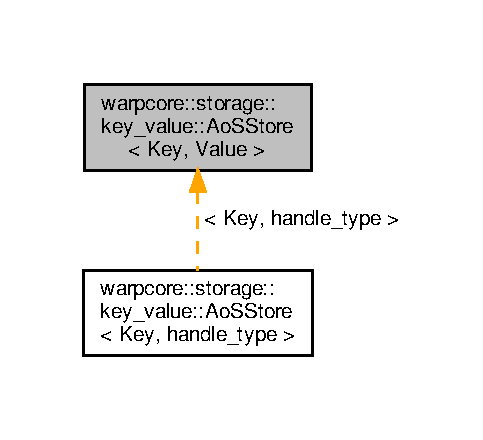
\includegraphics[width=232pt]{classwarpcore_1_1storage_1_1key__value_1_1AoSStore__inherit__graph}
\end{center}
\end{figure}
\subsection*{Public Types}
\begin{DoxyCompactItemize}
\item 
\mbox{\Hypertarget{classwarpcore_1_1storage_1_1key__value_1_1AoSStore_aa1c40f9e45e7d97e2926b6814ff32d1d}\label{classwarpcore_1_1storage_1_1key__value_1_1AoSStore_aa1c40f9e45e7d97e2926b6814ff32d1d}} 
using {\bfseries key\+\_\+type} = Key
\item 
\mbox{\Hypertarget{classwarpcore_1_1storage_1_1key__value_1_1AoSStore_acbd77ee61a9caa4ef1c82bb0212abc02}\label{classwarpcore_1_1storage_1_1key__value_1_1AoSStore_acbd77ee61a9caa4ef1c82bb0212abc02}} 
using {\bfseries value\+\_\+type} = Value
\item 
\mbox{\Hypertarget{classwarpcore_1_1storage_1_1key__value_1_1AoSStore_aeb90dbd4f0de6218c8110dec7a519bc0}\label{classwarpcore_1_1storage_1_1key__value_1_1AoSStore_aeb90dbd4f0de6218c8110dec7a519bc0}} 
using {\bfseries status\+\_\+type} = \hyperlink{classwarpcore_1_1Status}{Status}
\item 
\mbox{\Hypertarget{classwarpcore_1_1storage_1_1key__value_1_1AoSStore_a772de3b52743e24640208288c60f9c1b}\label{classwarpcore_1_1storage_1_1key__value_1_1AoSStore_a772de3b52743e24640208288c60f9c1b}} 
using {\bfseries index\+\_\+type} = index\+\_\+t
\item 
\mbox{\Hypertarget{classwarpcore_1_1storage_1_1key__value_1_1AoSStore_a73fe24ae74a4f202a08aab194ec82da3}\label{classwarpcore_1_1storage_1_1key__value_1_1AoSStore_a73fe24ae74a4f202a08aab194ec82da3}} 
using {\bfseries tag} = tags\+::key\+\_\+value\+\_\+storage
\end{DoxyCompactItemize}
\subsection*{Public Member Functions}
\begin{DoxyCompactItemize}
\item 
\+\_\+\+\_\+host\+\_\+\+\_\+ \hyperlink{classwarpcore_1_1storage_1_1key__value_1_1AoSStore_a4ab568a9090dfe80c989ba7d88173010}{Ao\+S\+Store} (const index\+\_\+type \hyperlink{classwarpcore_1_1storage_1_1key__value_1_1AoSStore_a23c4cb728f870dfa09a0d0d976cedf8e}{capacity}) noexcept
\begin{DoxyCompactList}\small\item\em constructor \end{DoxyCompactList}\item 
\+\_\+\+\_\+host\+\_\+\+\_\+\+\_\+\+\_\+device\+\_\+\+\_\+ \hyperlink{classwarpcore_1_1storage_1_1key__value_1_1AoSStore_a55dc641ec2d9643973506f6ed0c4b817}{Ao\+S\+Store} (const \hyperlink{classwarpcore_1_1storage_1_1key__value_1_1AoSStore}{Ao\+S\+Store} \&o) noexcept
\begin{DoxyCompactList}\small\item\em copy-\/constructor (shallow) \end{DoxyCompactList}\item 
\+\_\+\+\_\+host\+\_\+\+\_\+ \hyperlink{classwarpcore_1_1storage_1_1key__value_1_1AoSStore_ae3eef233b7fd2dbfeedd90c72c119d29}{Ao\+S\+Store} (\hyperlink{classwarpcore_1_1storage_1_1key__value_1_1AoSStore}{Ao\+S\+Store} \&\&o) noexcept
\begin{DoxyCompactList}\small\item\em move-\/constructor \end{DoxyCompactList}\item 
\mbox{\Hypertarget{classwarpcore_1_1storage_1_1key__value_1_1AoSStore_a0007916878191e222fd831f379eac189}\label{classwarpcore_1_1storage_1_1key__value_1_1AoSStore_a0007916878191e222fd831f379eac189}} 
\+\_\+\+\_\+host\+\_\+\+\_\+ \hyperlink{classwarpcore_1_1storage_1_1key__value_1_1AoSStore_a0007916878191e222fd831f379eac189}{$\sim$\+Ao\+S\+Store} () noexcept
\begin{DoxyCompactList}\small\item\em destructor \end{DoxyCompactList}\item 
\+\_\+\+\_\+host\+\_\+\+\_\+ void \hyperlink{classwarpcore_1_1storage_1_1key__value_1_1AoSStore_abd88eb047b4435c11bb639df0e2fd7ee}{init\+\_\+keys} (const key\+\_\+type key, const cuda\+Stream\+\_\+t stream=0) noexcept
\begin{DoxyCompactList}\small\item\em initialize keys \end{DoxyCompactList}\item 
\+\_\+\+\_\+host\+\_\+\+\_\+ void \hyperlink{classwarpcore_1_1storage_1_1key__value_1_1AoSStore_ae38e88a4174cb42513ed2e0b0a521ce9}{init\+\_\+values} (const value\+\_\+type value, const cuda\+Stream\+\_\+t stream=0) noexcept
\begin{DoxyCompactList}\small\item\em initialize values \end{DoxyCompactList}\item 
\+\_\+\+\_\+host\+\_\+\+\_\+ void \hyperlink{classwarpcore_1_1storage_1_1key__value_1_1AoSStore_aa4a8c988799409be60ee3368014fc13d}{init\+\_\+pairs} (const key\+\_\+type key, const value\+\_\+type value, const cuda\+Stream\+\_\+t stream=0) noexcept
\begin{DoxyCompactList}\small\item\em initialize key/value pairs \end{DoxyCompactList}\item 
\+\_\+\+\_\+device\+\_\+\+\_\+ pair\+\_\+t \& \hyperlink{classwarpcore_1_1storage_1_1key__value_1_1AoSStore_a786abe7fc9dfef28f1307f32a22fcb82}{operator\mbox{[}$\,$\mbox{]}} (const index\+\_\+type i) noexcept
\begin{DoxyCompactList}\small\item\em accessor \end{DoxyCompactList}\item 
\+\_\+\+\_\+device\+\_\+\+\_\+ const pair\+\_\+t \& \hyperlink{classwarpcore_1_1storage_1_1key__value_1_1AoSStore_abbae46c24d02a8a0bb74322496658d1b}{operator\mbox{[}$\,$\mbox{]}} (const index\+\_\+type i) const noexcept
\begin{DoxyCompactList}\small\item\em const accessor \end{DoxyCompactList}\item 
\+\_\+\+\_\+host\+\_\+\+\_\+\+\_\+\+\_\+device\+\_\+\+\_\+ \hyperlink{classwarpcore_1_1Status}{status\+\_\+type} \hyperlink{classwarpcore_1_1storage_1_1key__value_1_1AoSStore_a040cd6b5abf7ad6b2f20d44d5bae38bf}{status} () const noexcept
\begin{DoxyCompactList}\small\item\em get storage status \end{DoxyCompactList}\item 
\+\_\+\+\_\+host\+\_\+\+\_\+\+\_\+\+\_\+device\+\_\+\+\_\+ index\+\_\+type \hyperlink{classwarpcore_1_1storage_1_1key__value_1_1AoSStore_a23c4cb728f870dfa09a0d0d976cedf8e}{capacity} () const noexcept
\begin{DoxyCompactList}\small\item\em get storage capacity \end{DoxyCompactList}\item 
\+\_\+\+\_\+host\+\_\+\+\_\+ index\+\_\+type \hyperlink{classwarpcore_1_1storage_1_1key__value_1_1AoSStore_afe4d4e5048411c0d09a625c6447c19b6}{bytes\+\_\+total} () const noexcept
\begin{DoxyCompactList}\small\item\em get the total number of bytes occupied by this data structure \end{DoxyCompactList}\end{DoxyCompactItemize}


\subsection{Detailed Description}
\subsubsection*{template$<$class Key, class Value$>$\newline
class warpcore\+::storage\+::key\+\_\+value\+::\+Ao\+S\+Store$<$ Key, Value $>$}

key/value store with array-\/of-\/structs memory layout 


\begin{DoxyTemplParams}{Template Parameters}
{\em Key} & key type \\
\hline
{\em Value} & value type \\
\hline
\end{DoxyTemplParams}


\subsection{Constructor \& Destructor Documentation}
\mbox{\Hypertarget{classwarpcore_1_1storage_1_1key__value_1_1AoSStore_a4ab568a9090dfe80c989ba7d88173010}\label{classwarpcore_1_1storage_1_1key__value_1_1AoSStore_a4ab568a9090dfe80c989ba7d88173010}} 
\index{warpcore\+::storage\+::key\+\_\+value\+::\+Ao\+S\+Store@{warpcore\+::storage\+::key\+\_\+value\+::\+Ao\+S\+Store}!Ao\+S\+Store@{Ao\+S\+Store}}
\index{Ao\+S\+Store@{Ao\+S\+Store}!warpcore\+::storage\+::key\+\_\+value\+::\+Ao\+S\+Store@{warpcore\+::storage\+::key\+\_\+value\+::\+Ao\+S\+Store}}
\subsubsection{\texorpdfstring{Ao\+S\+Store()}{AoSStore()}\hspace{0.1cm}{\footnotesize\ttfamily [1/3]}}
{\footnotesize\ttfamily template$<$class Key, class Value$>$ \\
\+\_\+\+\_\+host\+\_\+\+\_\+ \hyperlink{classwarpcore_1_1storage_1_1key__value_1_1AoSStore}{warpcore\+::storage\+::key\+\_\+value\+::\+Ao\+S\+Store}$<$ Key, Value $>$\+::\hyperlink{classwarpcore_1_1storage_1_1key__value_1_1AoSStore}{Ao\+S\+Store} (\begin{DoxyParamCaption}\item[{const index\+\_\+type}]{capacity }\end{DoxyParamCaption})\hspace{0.3cm}{\ttfamily [inline]}, {\ttfamily [explicit]}, {\ttfamily [noexcept]}}



constructor 


\begin{DoxyParams}[1]{Parameters}
\mbox{\tt in}  & {\em capacity} & number of key/value slots \\
\hline
\end{DoxyParams}
\mbox{\Hypertarget{classwarpcore_1_1storage_1_1key__value_1_1AoSStore_a55dc641ec2d9643973506f6ed0c4b817}\label{classwarpcore_1_1storage_1_1key__value_1_1AoSStore_a55dc641ec2d9643973506f6ed0c4b817}} 
\index{warpcore\+::storage\+::key\+\_\+value\+::\+Ao\+S\+Store@{warpcore\+::storage\+::key\+\_\+value\+::\+Ao\+S\+Store}!Ao\+S\+Store@{Ao\+S\+Store}}
\index{Ao\+S\+Store@{Ao\+S\+Store}!warpcore\+::storage\+::key\+\_\+value\+::\+Ao\+S\+Store@{warpcore\+::storage\+::key\+\_\+value\+::\+Ao\+S\+Store}}
\subsubsection{\texorpdfstring{Ao\+S\+Store()}{AoSStore()}\hspace{0.1cm}{\footnotesize\ttfamily [2/3]}}
{\footnotesize\ttfamily template$<$class Key, class Value$>$ \\
\+\_\+\+\_\+host\+\_\+\+\_\+\+\_\+\+\_\+device\+\_\+\+\_\+ \hyperlink{classwarpcore_1_1storage_1_1key__value_1_1AoSStore}{warpcore\+::storage\+::key\+\_\+value\+::\+Ao\+S\+Store}$<$ Key, Value $>$\+::\hyperlink{classwarpcore_1_1storage_1_1key__value_1_1AoSStore}{Ao\+S\+Store} (\begin{DoxyParamCaption}\item[{const \hyperlink{classwarpcore_1_1storage_1_1key__value_1_1AoSStore}{Ao\+S\+Store}$<$ Key, Value $>$ \&}]{o }\end{DoxyParamCaption})\hspace{0.3cm}{\ttfamily [inline]}, {\ttfamily [noexcept]}}



copy-\/constructor (shallow) 


\begin{DoxyParams}[1]{Parameters}
\mbox{\tt in}  & {\em object} & to be copied \\
\hline
\end{DoxyParams}
\mbox{\Hypertarget{classwarpcore_1_1storage_1_1key__value_1_1AoSStore_ae3eef233b7fd2dbfeedd90c72c119d29}\label{classwarpcore_1_1storage_1_1key__value_1_1AoSStore_ae3eef233b7fd2dbfeedd90c72c119d29}} 
\index{warpcore\+::storage\+::key\+\_\+value\+::\+Ao\+S\+Store@{warpcore\+::storage\+::key\+\_\+value\+::\+Ao\+S\+Store}!Ao\+S\+Store@{Ao\+S\+Store}}
\index{Ao\+S\+Store@{Ao\+S\+Store}!warpcore\+::storage\+::key\+\_\+value\+::\+Ao\+S\+Store@{warpcore\+::storage\+::key\+\_\+value\+::\+Ao\+S\+Store}}
\subsubsection{\texorpdfstring{Ao\+S\+Store()}{AoSStore()}\hspace{0.1cm}{\footnotesize\ttfamily [3/3]}}
{\footnotesize\ttfamily template$<$class Key, class Value$>$ \\
\+\_\+\+\_\+host\+\_\+\+\_\+ \hyperlink{classwarpcore_1_1storage_1_1key__value_1_1AoSStore}{warpcore\+::storage\+::key\+\_\+value\+::\+Ao\+S\+Store}$<$ Key, Value $>$\+::\hyperlink{classwarpcore_1_1storage_1_1key__value_1_1AoSStore}{Ao\+S\+Store} (\begin{DoxyParamCaption}\item[{\hyperlink{classwarpcore_1_1storage_1_1key__value_1_1AoSStore}{Ao\+S\+Store}$<$ Key, Value $>$ \&\&}]{o }\end{DoxyParamCaption})\hspace{0.3cm}{\ttfamily [inline]}, {\ttfamily [noexcept]}}



move-\/constructor 


\begin{DoxyParams}[1]{Parameters}
\mbox{\tt in}  & {\em object} & to be moved \\
\hline
\end{DoxyParams}


\subsection{Member Function Documentation}
\mbox{\Hypertarget{classwarpcore_1_1storage_1_1key__value_1_1AoSStore_afe4d4e5048411c0d09a625c6447c19b6}\label{classwarpcore_1_1storage_1_1key__value_1_1AoSStore_afe4d4e5048411c0d09a625c6447c19b6}} 
\index{warpcore\+::storage\+::key\+\_\+value\+::\+Ao\+S\+Store@{warpcore\+::storage\+::key\+\_\+value\+::\+Ao\+S\+Store}!bytes\+\_\+total@{bytes\+\_\+total}}
\index{bytes\+\_\+total@{bytes\+\_\+total}!warpcore\+::storage\+::key\+\_\+value\+::\+Ao\+S\+Store@{warpcore\+::storage\+::key\+\_\+value\+::\+Ao\+S\+Store}}
\subsubsection{\texorpdfstring{bytes\+\_\+total()}{bytes\_total()}}
{\footnotesize\ttfamily template$<$class Key, class Value$>$ \\
\+\_\+\+\_\+host\+\_\+\+\_\+ index\+\_\+type \hyperlink{classwarpcore_1_1storage_1_1key__value_1_1AoSStore}{warpcore\+::storage\+::key\+\_\+value\+::\+Ao\+S\+Store}$<$ Key, Value $>$\+::bytes\+\_\+total (\begin{DoxyParamCaption}{ }\end{DoxyParamCaption}) const\hspace{0.3cm}{\ttfamily [inline]}, {\ttfamily [noexcept]}}



get the total number of bytes occupied by this data structure 

\begin{DoxyReturn}{Returns}
bytes 
\end{DoxyReturn}
\mbox{\Hypertarget{classwarpcore_1_1storage_1_1key__value_1_1AoSStore_a23c4cb728f870dfa09a0d0d976cedf8e}\label{classwarpcore_1_1storage_1_1key__value_1_1AoSStore_a23c4cb728f870dfa09a0d0d976cedf8e}} 
\index{warpcore\+::storage\+::key\+\_\+value\+::\+Ao\+S\+Store@{warpcore\+::storage\+::key\+\_\+value\+::\+Ao\+S\+Store}!capacity@{capacity}}
\index{capacity@{capacity}!warpcore\+::storage\+::key\+\_\+value\+::\+Ao\+S\+Store@{warpcore\+::storage\+::key\+\_\+value\+::\+Ao\+S\+Store}}
\subsubsection{\texorpdfstring{capacity()}{capacity()}}
{\footnotesize\ttfamily template$<$class Key, class Value$>$ \\
\+\_\+\+\_\+host\+\_\+\+\_\+\+\_\+\+\_\+device\+\_\+\+\_\+ index\+\_\+type \hyperlink{classwarpcore_1_1storage_1_1key__value_1_1AoSStore}{warpcore\+::storage\+::key\+\_\+value\+::\+Ao\+S\+Store}$<$ Key, Value $>$\+::capacity (\begin{DoxyParamCaption}{ }\end{DoxyParamCaption}) const\hspace{0.3cm}{\ttfamily [inline]}, {\ttfamily [noexcept]}}



get storage capacity 

\begin{DoxyReturn}{Returns}
status 
\end{DoxyReturn}
\mbox{\Hypertarget{classwarpcore_1_1storage_1_1key__value_1_1AoSStore_abd88eb047b4435c11bb639df0e2fd7ee}\label{classwarpcore_1_1storage_1_1key__value_1_1AoSStore_abd88eb047b4435c11bb639df0e2fd7ee}} 
\index{warpcore\+::storage\+::key\+\_\+value\+::\+Ao\+S\+Store@{warpcore\+::storage\+::key\+\_\+value\+::\+Ao\+S\+Store}!init\+\_\+keys@{init\+\_\+keys}}
\index{init\+\_\+keys@{init\+\_\+keys}!warpcore\+::storage\+::key\+\_\+value\+::\+Ao\+S\+Store@{warpcore\+::storage\+::key\+\_\+value\+::\+Ao\+S\+Store}}
\subsubsection{\texorpdfstring{init\+\_\+keys()}{init\_keys()}}
{\footnotesize\ttfamily template$<$class Key, class Value$>$ \\
\+\_\+\+\_\+host\+\_\+\+\_\+ void \hyperlink{classwarpcore_1_1storage_1_1key__value_1_1AoSStore}{warpcore\+::storage\+::key\+\_\+value\+::\+Ao\+S\+Store}$<$ Key, Value $>$\+::init\+\_\+keys (\begin{DoxyParamCaption}\item[{const key\+\_\+type}]{key,  }\item[{const cuda\+Stream\+\_\+t}]{stream = {\ttfamily 0} }\end{DoxyParamCaption})\hspace{0.3cm}{\ttfamily [inline]}, {\ttfamily [noexcept]}}



initialize keys 


\begin{DoxyParams}[1]{Parameters}
\mbox{\tt in}  & {\em key} & initializer key \\
\hline
\mbox{\tt in}  & {\em stream} & C\+U\+DA stream in which this operation is executed in \\
\hline
\end{DoxyParams}
\mbox{\Hypertarget{classwarpcore_1_1storage_1_1key__value_1_1AoSStore_aa4a8c988799409be60ee3368014fc13d}\label{classwarpcore_1_1storage_1_1key__value_1_1AoSStore_aa4a8c988799409be60ee3368014fc13d}} 
\index{warpcore\+::storage\+::key\+\_\+value\+::\+Ao\+S\+Store@{warpcore\+::storage\+::key\+\_\+value\+::\+Ao\+S\+Store}!init\+\_\+pairs@{init\+\_\+pairs}}
\index{init\+\_\+pairs@{init\+\_\+pairs}!warpcore\+::storage\+::key\+\_\+value\+::\+Ao\+S\+Store@{warpcore\+::storage\+::key\+\_\+value\+::\+Ao\+S\+Store}}
\subsubsection{\texorpdfstring{init\+\_\+pairs()}{init\_pairs()}}
{\footnotesize\ttfamily template$<$class Key, class Value$>$ \\
\+\_\+\+\_\+host\+\_\+\+\_\+ void \hyperlink{classwarpcore_1_1storage_1_1key__value_1_1AoSStore}{warpcore\+::storage\+::key\+\_\+value\+::\+Ao\+S\+Store}$<$ Key, Value $>$\+::init\+\_\+pairs (\begin{DoxyParamCaption}\item[{const key\+\_\+type}]{key,  }\item[{const value\+\_\+type}]{value,  }\item[{const cuda\+Stream\+\_\+t}]{stream = {\ttfamily 0} }\end{DoxyParamCaption})\hspace{0.3cm}{\ttfamily [inline]}, {\ttfamily [noexcept]}}



initialize key/value pairs 


\begin{DoxyParams}[1]{Parameters}
\mbox{\tt in}  & {\em key} & initializer key \\
\hline
\mbox{\tt in}  & {\em value} & initializer value \\
\hline
\mbox{\tt in}  & {\em stream} & C\+U\+DA stream in which this operation is executed in \\
\hline
\end{DoxyParams}
\mbox{\Hypertarget{classwarpcore_1_1storage_1_1key__value_1_1AoSStore_ae38e88a4174cb42513ed2e0b0a521ce9}\label{classwarpcore_1_1storage_1_1key__value_1_1AoSStore_ae38e88a4174cb42513ed2e0b0a521ce9}} 
\index{warpcore\+::storage\+::key\+\_\+value\+::\+Ao\+S\+Store@{warpcore\+::storage\+::key\+\_\+value\+::\+Ao\+S\+Store}!init\+\_\+values@{init\+\_\+values}}
\index{init\+\_\+values@{init\+\_\+values}!warpcore\+::storage\+::key\+\_\+value\+::\+Ao\+S\+Store@{warpcore\+::storage\+::key\+\_\+value\+::\+Ao\+S\+Store}}
\subsubsection{\texorpdfstring{init\+\_\+values()}{init\_values()}}
{\footnotesize\ttfamily template$<$class Key, class Value$>$ \\
\+\_\+\+\_\+host\+\_\+\+\_\+ void \hyperlink{classwarpcore_1_1storage_1_1key__value_1_1AoSStore}{warpcore\+::storage\+::key\+\_\+value\+::\+Ao\+S\+Store}$<$ Key, Value $>$\+::init\+\_\+values (\begin{DoxyParamCaption}\item[{const value\+\_\+type}]{value,  }\item[{const cuda\+Stream\+\_\+t}]{stream = {\ttfamily 0} }\end{DoxyParamCaption})\hspace{0.3cm}{\ttfamily [inline]}, {\ttfamily [noexcept]}}



initialize values 


\begin{DoxyParams}[1]{Parameters}
\mbox{\tt in}  & {\em value} & initializer value \\
\hline
\mbox{\tt in}  & {\em stream} & C\+U\+DA stream in which this operation is executed in \\
\hline
\end{DoxyParams}
\mbox{\Hypertarget{classwarpcore_1_1storage_1_1key__value_1_1AoSStore_a786abe7fc9dfef28f1307f32a22fcb82}\label{classwarpcore_1_1storage_1_1key__value_1_1AoSStore_a786abe7fc9dfef28f1307f32a22fcb82}} 
\index{warpcore\+::storage\+::key\+\_\+value\+::\+Ao\+S\+Store@{warpcore\+::storage\+::key\+\_\+value\+::\+Ao\+S\+Store}!operator\mbox{[}\mbox{]}@{operator[]}}
\index{operator\mbox{[}\mbox{]}@{operator[]}!warpcore\+::storage\+::key\+\_\+value\+::\+Ao\+S\+Store@{warpcore\+::storage\+::key\+\_\+value\+::\+Ao\+S\+Store}}
\subsubsection{\texorpdfstring{operator[]()}{operator[]()}\hspace{0.1cm}{\footnotesize\ttfamily [1/2]}}
{\footnotesize\ttfamily template$<$class Key, class Value$>$ \\
\+\_\+\+\_\+device\+\_\+\+\_\+ pair\+\_\+t\& \hyperlink{classwarpcore_1_1storage_1_1key__value_1_1AoSStore}{warpcore\+::storage\+::key\+\_\+value\+::\+Ao\+S\+Store}$<$ Key, Value $>$\+::operator\mbox{[}$\,$\mbox{]} (\begin{DoxyParamCaption}\item[{const index\+\_\+type}]{i }\end{DoxyParamCaption})\hspace{0.3cm}{\ttfamily [inline]}, {\ttfamily [noexcept]}}



accessor 


\begin{DoxyParams}[1]{Parameters}
\mbox{\tt in}  & {\em i} & index to access \\
\hline
\end{DoxyParams}
\begin{DoxyReturn}{Returns}
pair at position {\ttfamily i} 
\end{DoxyReturn}
\mbox{\Hypertarget{classwarpcore_1_1storage_1_1key__value_1_1AoSStore_abbae46c24d02a8a0bb74322496658d1b}\label{classwarpcore_1_1storage_1_1key__value_1_1AoSStore_abbae46c24d02a8a0bb74322496658d1b}} 
\index{warpcore\+::storage\+::key\+\_\+value\+::\+Ao\+S\+Store@{warpcore\+::storage\+::key\+\_\+value\+::\+Ao\+S\+Store}!operator\mbox{[}\mbox{]}@{operator[]}}
\index{operator\mbox{[}\mbox{]}@{operator[]}!warpcore\+::storage\+::key\+\_\+value\+::\+Ao\+S\+Store@{warpcore\+::storage\+::key\+\_\+value\+::\+Ao\+S\+Store}}
\subsubsection{\texorpdfstring{operator[]()}{operator[]()}\hspace{0.1cm}{\footnotesize\ttfamily [2/2]}}
{\footnotesize\ttfamily template$<$class Key, class Value$>$ \\
\+\_\+\+\_\+device\+\_\+\+\_\+ const pair\+\_\+t\& \hyperlink{classwarpcore_1_1storage_1_1key__value_1_1AoSStore}{warpcore\+::storage\+::key\+\_\+value\+::\+Ao\+S\+Store}$<$ Key, Value $>$\+::operator\mbox{[}$\,$\mbox{]} (\begin{DoxyParamCaption}\item[{const index\+\_\+type}]{i }\end{DoxyParamCaption}) const\hspace{0.3cm}{\ttfamily [inline]}, {\ttfamily [noexcept]}}



const accessor 


\begin{DoxyParams}[1]{Parameters}
\mbox{\tt in}  & {\em i} & index to access \\
\hline
\end{DoxyParams}
\begin{DoxyReturn}{Returns}
pair at position {\ttfamily i} 
\end{DoxyReturn}
\mbox{\Hypertarget{classwarpcore_1_1storage_1_1key__value_1_1AoSStore_a040cd6b5abf7ad6b2f20d44d5bae38bf}\label{classwarpcore_1_1storage_1_1key__value_1_1AoSStore_a040cd6b5abf7ad6b2f20d44d5bae38bf}} 
\index{warpcore\+::storage\+::key\+\_\+value\+::\+Ao\+S\+Store@{warpcore\+::storage\+::key\+\_\+value\+::\+Ao\+S\+Store}!status@{status}}
\index{status@{status}!warpcore\+::storage\+::key\+\_\+value\+::\+Ao\+S\+Store@{warpcore\+::storage\+::key\+\_\+value\+::\+Ao\+S\+Store}}
\subsubsection{\texorpdfstring{status()}{status()}}
{\footnotesize\ttfamily template$<$class Key, class Value$>$ \\
\+\_\+\+\_\+host\+\_\+\+\_\+\+\_\+\+\_\+device\+\_\+\+\_\+ \hyperlink{classwarpcore_1_1Status}{status\+\_\+type} \hyperlink{classwarpcore_1_1storage_1_1key__value_1_1AoSStore}{warpcore\+::storage\+::key\+\_\+value\+::\+Ao\+S\+Store}$<$ Key, Value $>$\+::status (\begin{DoxyParamCaption}{ }\end{DoxyParamCaption}) const\hspace{0.3cm}{\ttfamily [inline]}, {\ttfamily [noexcept]}}



get storage status 

\begin{DoxyReturn}{Returns}
status 
\end{DoxyReturn}

\hypertarget{classwarpcore_1_1BloomFilter}{}\section{warpcore\+:\+:Bloom\+Filter$<$ Key, Hasher, Slot, C\+G\+Size $>$ Class Template Reference}
\label{classwarpcore_1_1BloomFilter}\index{warpcore\+::\+Bloom\+Filter$<$ Key, Hasher, Slot, C\+G\+Size $>$@{warpcore\+::\+Bloom\+Filter$<$ Key, Hasher, Slot, C\+G\+Size $>$}}


bloom filter  


\subsection*{Public Types}
\begin{DoxyCompactItemize}
\item 
\mbox{\Hypertarget{classwarpcore_1_1BloomFilter_ae33a034a8dfe87aba6e92af1a210d943}\label{classwarpcore_1_1BloomFilter_ae33a034a8dfe87aba6e92af1a210d943}} 
using {\bfseries key\+\_\+type} = Key
\item 
\mbox{\Hypertarget{classwarpcore_1_1BloomFilter_a9eb144015fa06a5b481f9f5a872662af}\label{classwarpcore_1_1BloomFilter_a9eb144015fa06a5b481f9f5a872662af}} 
using {\bfseries value\+\_\+type} = bool
\item 
\mbox{\Hypertarget{classwarpcore_1_1BloomFilter_a95a1a6802d0de2f792372f81a0534bc4}\label{classwarpcore_1_1BloomFilter_a95a1a6802d0de2f792372f81a0534bc4}} 
using {\bfseries index\+\_\+type} = index\+\_\+t
\item 
\mbox{\Hypertarget{classwarpcore_1_1BloomFilter_a0f472c61b84dd8e07309064bdb8a8bdd}\label{classwarpcore_1_1BloomFilter_a0f472c61b84dd8e07309064bdb8a8bdd}} 
using {\bfseries slot\+\_\+type} = Slot
\item 
\mbox{\Hypertarget{classwarpcore_1_1BloomFilter_a6341f8816b7384983431a2229f28385f}\label{classwarpcore_1_1BloomFilter_a6341f8816b7384983431a2229f28385f}} 
using {\bfseries status\+\_\+type} = \hyperlink{classwarpcore_1_1Status}{Status}
\end{DoxyCompactItemize}
\subsection*{Public Member Functions}
\begin{DoxyCompactItemize}
\item 
\+\_\+\+\_\+host\+\_\+\+\_\+ \hyperlink{classwarpcore_1_1BloomFilter_a0050427179ed9b718800a42f9eeedb36}{Bloom\+Filter} (index\+\_\+type \hyperlink{classwarpcore_1_1BloomFilter_a54a25926cf770e834c47ad5164e91443}{num\+\_\+bits}, index\+\_\+type \hyperlink{classwarpcore_1_1BloomFilter_a33c972e8a462625d6253b58bbd5585f3}{k}, key\+\_\+type seed=defaults\+::seed$<$ key\+\_\+type $>$()) noexcept
\begin{DoxyCompactList}\small\item\em constructor \end{DoxyCompactList}\item 
\+\_\+\+\_\+host\+\_\+\+\_\+\+\_\+\+\_\+device\+\_\+\+\_\+ \hyperlink{classwarpcore_1_1BloomFilter_a883979f0bdf59e494c366eef343ea7b4}{Bloom\+Filter} (const \hyperlink{classwarpcore_1_1BloomFilter}{Bloom\+Filter} \&o) noexcept
\begin{DoxyCompactList}\small\item\em copy-\/constructor (shallow) \end{DoxyCompactList}\item 
\+\_\+\+\_\+host\+\_\+\+\_\+ \hyperlink{classwarpcore_1_1BloomFilter_aa0a03f44ed1c877335537a1e3fcb9208}{Bloom\+Filter} (\hyperlink{classwarpcore_1_1BloomFilter}{Bloom\+Filter} \&\&o) noexcept
\begin{DoxyCompactList}\small\item\em move-\/constructor \end{DoxyCompactList}\item 
\mbox{\Hypertarget{classwarpcore_1_1BloomFilter_a43381c51633999d04e0002c32885e3b7}\label{classwarpcore_1_1BloomFilter_a43381c51633999d04e0002c32885e3b7}} 
\+\_\+\+\_\+host\+\_\+\+\_\+ \hyperlink{classwarpcore_1_1BloomFilter_a43381c51633999d04e0002c32885e3b7}{$\sim$\+Bloom\+Filter} () noexcept
\begin{DoxyCompactList}\small\item\em destructor \end{DoxyCompactList}\item 
\+\_\+\+\_\+host\+\_\+\+\_\+ void \hyperlink{classwarpcore_1_1BloomFilter_ac9e663f21e94822fc214b75c623436f5}{init} (cuda\+Stream\+\_\+t stream=0) noexcept
\begin{DoxyCompactList}\small\item\em re-\/initialize the hash table \end{DoxyCompactList}\item 
\+\_\+\+\_\+device\+\_\+\+\_\+ void \hyperlink{classwarpcore_1_1BloomFilter_a8567325cd30886f3daf2c615a35bb02e}{insert} (key\+\_\+type key, const cg\+::thread\+\_\+block\+\_\+tile$<$ \hyperlink{classwarpcore_1_1BloomFilter_a6ad2335811852ad62fc65e85416d3904}{cg\+\_\+size}()$>$ \&group) noexcept
\begin{DoxyCompactList}\small\item\em inserts a key into the bloom filter \end{DoxyCompactList}\item 
\+\_\+\+\_\+host\+\_\+\+\_\+ void \hyperlink{classwarpcore_1_1BloomFilter_a462859be5ed949c82d37909b139271ee}{insert} (Key $\ast$keys\+\_\+in, index\+\_\+t size\+\_\+in, cuda\+Stream\+\_\+t stream=0) noexcept
\begin{DoxyCompactList}\small\item\em inserts a set of keys into the bloom filter \end{DoxyCompactList}\item 
\+\_\+\+\_\+device\+\_\+\+\_\+ bool \hyperlink{classwarpcore_1_1BloomFilter_a47ffce0fc70aa6bd7a0ed4b837fec1bd}{retrieve} (key\+\_\+type key, const cg\+::thread\+\_\+block\+\_\+tile$<$ \hyperlink{classwarpcore_1_1BloomFilter_a6ad2335811852ad62fc65e85416d3904}{cg\+\_\+size}()$>$ \&group) const noexcept
\begin{DoxyCompactList}\small\item\em retrieve a key \end{DoxyCompactList}\item 
\+\_\+\+\_\+host\+\_\+\+\_\+ void \hyperlink{classwarpcore_1_1BloomFilter_a38025d88272e7de413210efe745aa279}{retrieve} (key\+\_\+type $\ast$keys\+\_\+in, index\+\_\+type size\+\_\+in, bool $\ast$flags\+\_\+out, cuda\+Stream\+\_\+t stream=0) const noexcept
\begin{DoxyCompactList}\small\item\em retrieve a set of keys \end{DoxyCompactList}\item 
{\footnotesize template$<$index\+\_\+type C\+G\+Size\+\_\+ = cg\+\_\+size(), class  = std\+::enable\+\_\+if\+\_\+t$<$\+C\+G\+Size\+\_\+ == 1$>$$>$ }\\\+\_\+\+\_\+device\+\_\+\+\_\+ bool \hyperlink{classwarpcore_1_1BloomFilter_a6dc903341218173f276cc855ba683ad1}{insert\+\_\+and\+\_\+query} (key\+\_\+type key, const cg\+::thread\+\_\+block\+\_\+tile$<$ \hyperlink{classwarpcore_1_1BloomFilter_a6ad2335811852ad62fc65e85416d3904}{cg\+\_\+size}()$>$ \&group) noexcept
\begin{DoxyCompactList}\small\item\em queries and subsequently inserts a key into the bloom filter \end{DoxyCompactList}\item 
\+\_\+\+\_\+host\+\_\+\+\_\+\+\_\+\+\_\+device\+\_\+\+\_\+ index\+\_\+type \hyperlink{classwarpcore_1_1BloomFilter_a54a25926cf770e834c47ad5164e91443}{num\+\_\+bits} () const noexcept
\begin{DoxyCompactList}\small\item\em get number of bits (m) \end{DoxyCompactList}\item 
\+\_\+\+\_\+host\+\_\+\+\_\+\+\_\+\+\_\+device\+\_\+\+\_\+ index\+\_\+type \hyperlink{classwarpcore_1_1BloomFilter_a1ab7ecd7bcc3f6321a252f94d63965eb}{num\+\_\+slots} () const noexcept
\begin{DoxyCompactList}\small\item\em get number of slots \end{DoxyCompactList}\item 
\+\_\+\+\_\+host\+\_\+\+\_\+\+\_\+\+\_\+device\+\_\+\+\_\+ index\+\_\+type \hyperlink{classwarpcore_1_1BloomFilter_a10fcbb540441eff40a1d0fccd1b992bd}{num\+\_\+blocks} () const noexcept
\begin{DoxyCompactList}\small\item\em get number of blocks \end{DoxyCompactList}\item 
\+\_\+\+\_\+host\+\_\+\+\_\+\+\_\+\+\_\+device\+\_\+\+\_\+ index\+\_\+type \hyperlink{classwarpcore_1_1BloomFilter_a33c972e8a462625d6253b58bbd5585f3}{k} () const noexcept
\begin{DoxyCompactList}\small\item\em get number of hash functions (k) \end{DoxyCompactList}\item 
\+\_\+\+\_\+host\+\_\+\+\_\+ double \hyperlink{classwarpcore_1_1BloomFilter_af77c52ec3c2223cfe335a65197bed625}{fpr} (index\+\_\+type n) const noexcept
\begin{DoxyCompactList}\small\item\em estimated false positive rate of pattern-\/blocked bloom filter \end{DoxyCompactList}\item 
\+\_\+\+\_\+host\+\_\+\+\_\+\+\_\+\+\_\+device\+\_\+\+\_\+ bool \hyperlink{classwarpcore_1_1BloomFilter_a55aaae73d8a1a8d811779fcf372f6c8c}{is\+\_\+copy} () const noexcept
\begin{DoxyCompactList}\small\item\em indicates if this object is a shallow copy \end{DoxyCompactList}\end{DoxyCompactItemize}
\subsection*{Static Public Member Functions}
\begin{DoxyCompactItemize}
\item 
static \+\_\+\+\_\+host\+\_\+\+\_\+\+\_\+\+\_\+device\+\_\+\+\_\+ constexpr index\+\_\+type \hyperlink{classwarpcore_1_1BloomFilter_a6ad2335811852ad62fc65e85416d3904}{cg\+\_\+size} () noexcept
\begin{DoxyCompactList}\small\item\em get cooperative group size \end{DoxyCompactList}\item 
static \+\_\+\+\_\+host\+\_\+\+\_\+\+\_\+\+\_\+device\+\_\+\+\_\+ constexpr index\+\_\+type \hyperlink{classwarpcore_1_1BloomFilter_a8dca50765c601cca8d85621fa8488ecc}{slot\+\_\+bits} () noexcept
\begin{DoxyCompactList}\small\item\em get bits per slot \end{DoxyCompactList}\item 
static \+\_\+\+\_\+host\+\_\+\+\_\+\+\_\+\+\_\+device\+\_\+\+\_\+ constexpr index\+\_\+type \hyperlink{classwarpcore_1_1BloomFilter_ae7d326580b41b88db73264a494db3a06}{block\+\_\+bits} () noexcept
\begin{DoxyCompactList}\small\item\em get bits per cooperative group block of slots \end{DoxyCompactList}\end{DoxyCompactItemize}


\subsection{Detailed Description}
\subsubsection*{template$<$class Key, class Hasher = defaults\+::hasher\+\_\+t$<$\+Key$>$, class Slot = std\+::uint64\+\_\+t, index\+\_\+t C\+G\+Size = 1$>$\newline
class warpcore\+::\+Bloom\+Filter$<$ Key, Hasher, Slot, C\+G\+Size $>$}

bloom filter 


\begin{DoxyTemplParams}{Template Parameters}
{\em Key} & key type ({\ttfamily std\+::uint32\+\_\+t} or {\ttfamily std\+::uint64\+\_\+t}) \\
\hline
{\em Hasher} & hasher from {\ttfamily \hyperlink{namespacewarpcore_1_1hashers}{warpcore\+::hashers}} \\
\hline
{\em Slot} & slot type ({\ttfamily std\+::uint32\+\_\+t} or {\ttfamily std\+::uint64\+\_\+t}) \\
\hline
{\em C\+G\+Size} & size of cooperative group \\
\hline
\end{DoxyTemplParams}


\subsection{Constructor \& Destructor Documentation}
\mbox{\Hypertarget{classwarpcore_1_1BloomFilter_a0050427179ed9b718800a42f9eeedb36}\label{classwarpcore_1_1BloomFilter_a0050427179ed9b718800a42f9eeedb36}} 
\index{warpcore\+::\+Bloom\+Filter@{warpcore\+::\+Bloom\+Filter}!Bloom\+Filter@{Bloom\+Filter}}
\index{Bloom\+Filter@{Bloom\+Filter}!warpcore\+::\+Bloom\+Filter@{warpcore\+::\+Bloom\+Filter}}
\subsubsection{\texorpdfstring{Bloom\+Filter()}{BloomFilter()}\hspace{0.1cm}{\footnotesize\ttfamily [1/3]}}
{\footnotesize\ttfamily template$<$class Key , class Hasher  = defaults\+::hasher\+\_\+t$<$\+Key$>$, class Slot  = std\+::uint64\+\_\+t, index\+\_\+t C\+G\+Size = 1$>$ \\
\+\_\+\+\_\+host\+\_\+\+\_\+ \hyperlink{classwarpcore_1_1BloomFilter}{warpcore\+::\+Bloom\+Filter}$<$ Key, Hasher, Slot, C\+G\+Size $>$\+::\hyperlink{classwarpcore_1_1BloomFilter}{Bloom\+Filter} (\begin{DoxyParamCaption}\item[{index\+\_\+type}]{num\+\_\+bits,  }\item[{index\+\_\+type}]{k,  }\item[{key\+\_\+type}]{seed = {\ttfamily defaults\+:\+:seed$<$key\+\_\+type$>$()} }\end{DoxyParamCaption})\hspace{0.3cm}{\ttfamily [inline]}, {\ttfamily [explicit]}, {\ttfamily [noexcept]}}



constructor 


\begin{DoxyParams}[1]{Parameters}
\mbox{\tt in}  & {\em num\+\_\+bits} & total number of bits (m) of the bloom filter \\
\hline
\mbox{\tt in}  & {\em k} & number of hash functions to apply \\
\hline
\mbox{\tt in}  & {\em seed} & random seed \\
\hline
\end{DoxyParams}
Here is the call graph for this function\+:
\nopagebreak
\begin{figure}[H]
\begin{center}
\leavevmode
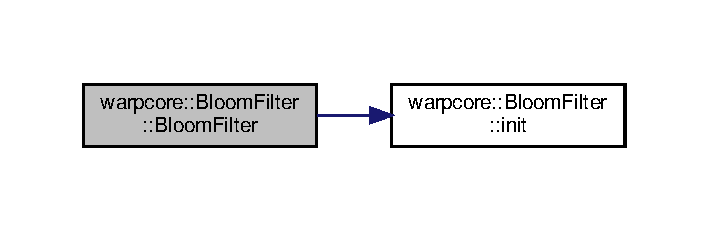
\includegraphics[width=340pt]{classwarpcore_1_1BloomFilter_a0050427179ed9b718800a42f9eeedb36_cgraph}
\end{center}
\end{figure}
\mbox{\Hypertarget{classwarpcore_1_1BloomFilter_a883979f0bdf59e494c366eef343ea7b4}\label{classwarpcore_1_1BloomFilter_a883979f0bdf59e494c366eef343ea7b4}} 
\index{warpcore\+::\+Bloom\+Filter@{warpcore\+::\+Bloom\+Filter}!Bloom\+Filter@{Bloom\+Filter}}
\index{Bloom\+Filter@{Bloom\+Filter}!warpcore\+::\+Bloom\+Filter@{warpcore\+::\+Bloom\+Filter}}
\subsubsection{\texorpdfstring{Bloom\+Filter()}{BloomFilter()}\hspace{0.1cm}{\footnotesize\ttfamily [2/3]}}
{\footnotesize\ttfamily template$<$class Key , class Hasher  = defaults\+::hasher\+\_\+t$<$\+Key$>$, class Slot  = std\+::uint64\+\_\+t, index\+\_\+t C\+G\+Size = 1$>$ \\
\+\_\+\+\_\+host\+\_\+\+\_\+\+\_\+\+\_\+device\+\_\+\+\_\+ \hyperlink{classwarpcore_1_1BloomFilter}{warpcore\+::\+Bloom\+Filter}$<$ Key, Hasher, Slot, C\+G\+Size $>$\+::\hyperlink{classwarpcore_1_1BloomFilter}{Bloom\+Filter} (\begin{DoxyParamCaption}\item[{const \hyperlink{classwarpcore_1_1BloomFilter}{Bloom\+Filter}$<$ Key, Hasher, Slot, C\+G\+Size $>$ \&}]{o }\end{DoxyParamCaption})\hspace{0.3cm}{\ttfamily [inline]}, {\ttfamily [noexcept]}}



copy-\/constructor (shallow) 


\begin{DoxyParams}[1]{Parameters}
\mbox{\tt in}  & {\em object} & to be copied \\
\hline
\end{DoxyParams}
\mbox{\Hypertarget{classwarpcore_1_1BloomFilter_aa0a03f44ed1c877335537a1e3fcb9208}\label{classwarpcore_1_1BloomFilter_aa0a03f44ed1c877335537a1e3fcb9208}} 
\index{warpcore\+::\+Bloom\+Filter@{warpcore\+::\+Bloom\+Filter}!Bloom\+Filter@{Bloom\+Filter}}
\index{Bloom\+Filter@{Bloom\+Filter}!warpcore\+::\+Bloom\+Filter@{warpcore\+::\+Bloom\+Filter}}
\subsubsection{\texorpdfstring{Bloom\+Filter()}{BloomFilter()}\hspace{0.1cm}{\footnotesize\ttfamily [3/3]}}
{\footnotesize\ttfamily template$<$class Key , class Hasher  = defaults\+::hasher\+\_\+t$<$\+Key$>$, class Slot  = std\+::uint64\+\_\+t, index\+\_\+t C\+G\+Size = 1$>$ \\
\+\_\+\+\_\+host\+\_\+\+\_\+ \hyperlink{classwarpcore_1_1BloomFilter}{warpcore\+::\+Bloom\+Filter}$<$ Key, Hasher, Slot, C\+G\+Size $>$\+::\hyperlink{classwarpcore_1_1BloomFilter}{Bloom\+Filter} (\begin{DoxyParamCaption}\item[{\hyperlink{classwarpcore_1_1BloomFilter}{Bloom\+Filter}$<$ Key, Hasher, Slot, C\+G\+Size $>$ \&\&}]{o }\end{DoxyParamCaption})\hspace{0.3cm}{\ttfamily [inline]}, {\ttfamily [noexcept]}}



move-\/constructor 


\begin{DoxyParams}[1]{Parameters}
\mbox{\tt in}  & {\em object} & to be moved \\
\hline
\end{DoxyParams}


\subsection{Member Function Documentation}
\mbox{\Hypertarget{classwarpcore_1_1BloomFilter_ae7d326580b41b88db73264a494db3a06}\label{classwarpcore_1_1BloomFilter_ae7d326580b41b88db73264a494db3a06}} 
\index{warpcore\+::\+Bloom\+Filter@{warpcore\+::\+Bloom\+Filter}!block\+\_\+bits@{block\+\_\+bits}}
\index{block\+\_\+bits@{block\+\_\+bits}!warpcore\+::\+Bloom\+Filter@{warpcore\+::\+Bloom\+Filter}}
\subsubsection{\texorpdfstring{block\+\_\+bits()}{block\_bits()}}
{\footnotesize\ttfamily template$<$class Key , class Hasher  = defaults\+::hasher\+\_\+t$<$\+Key$>$, class Slot  = std\+::uint64\+\_\+t, index\+\_\+t C\+G\+Size = 1$>$ \\
static \+\_\+\+\_\+host\+\_\+\+\_\+\+\_\+\+\_\+device\+\_\+\+\_\+ constexpr index\+\_\+type \hyperlink{classwarpcore_1_1BloomFilter}{warpcore\+::\+Bloom\+Filter}$<$ Key, Hasher, Slot, C\+G\+Size $>$\+::block\+\_\+bits (\begin{DoxyParamCaption}{ }\end{DoxyParamCaption})\hspace{0.3cm}{\ttfamily [inline]}, {\ttfamily [static]}, {\ttfamily [noexcept]}}



get bits per cooperative group block of slots 

\begin{DoxyReturn}{Returns}
number of bits 
\end{DoxyReturn}
Here is the call graph for this function\+:
\nopagebreak
\begin{figure}[H]
\begin{center}
\leavevmode
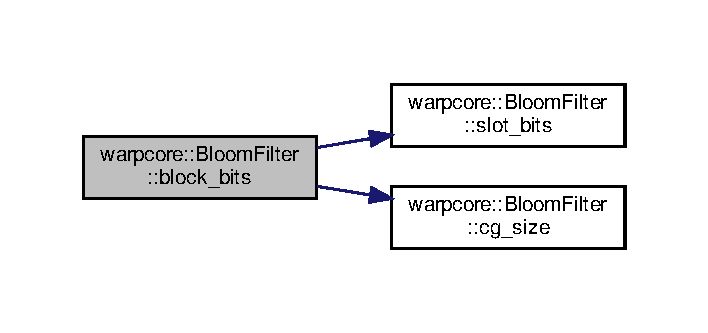
\includegraphics[width=340pt]{classwarpcore_1_1BloomFilter_ae7d326580b41b88db73264a494db3a06_cgraph}
\end{center}
\end{figure}
Here is the caller graph for this function\+:
\nopagebreak
\begin{figure}[H]
\begin{center}
\leavevmode
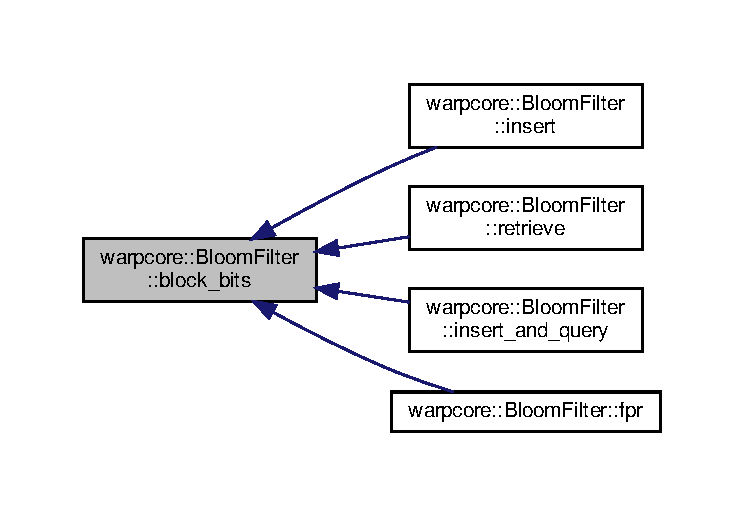
\includegraphics[width=350pt]{classwarpcore_1_1BloomFilter_ae7d326580b41b88db73264a494db3a06_icgraph}
\end{center}
\end{figure}
\mbox{\Hypertarget{classwarpcore_1_1BloomFilter_a6ad2335811852ad62fc65e85416d3904}\label{classwarpcore_1_1BloomFilter_a6ad2335811852ad62fc65e85416d3904}} 
\index{warpcore\+::\+Bloom\+Filter@{warpcore\+::\+Bloom\+Filter}!cg\+\_\+size@{cg\+\_\+size}}
\index{cg\+\_\+size@{cg\+\_\+size}!warpcore\+::\+Bloom\+Filter@{warpcore\+::\+Bloom\+Filter}}
\subsubsection{\texorpdfstring{cg\+\_\+size()}{cg\_size()}}
{\footnotesize\ttfamily template$<$class Key , class Hasher  = defaults\+::hasher\+\_\+t$<$\+Key$>$, class Slot  = std\+::uint64\+\_\+t, index\+\_\+t C\+G\+Size = 1$>$ \\
static \+\_\+\+\_\+host\+\_\+\+\_\+\+\_\+\+\_\+device\+\_\+\+\_\+ constexpr index\+\_\+type \hyperlink{classwarpcore_1_1BloomFilter}{warpcore\+::\+Bloom\+Filter}$<$ Key, Hasher, Slot, C\+G\+Size $>$\+::cg\+\_\+size (\begin{DoxyParamCaption}{ }\end{DoxyParamCaption})\hspace{0.3cm}{\ttfamily [inline]}, {\ttfamily [static]}, {\ttfamily [noexcept]}}



get cooperative group size 

\begin{DoxyReturn}{Returns}
cooperative group size 
\end{DoxyReturn}
Here is the caller graph for this function\+:
\nopagebreak
\begin{figure}[H]
\begin{center}
\leavevmode
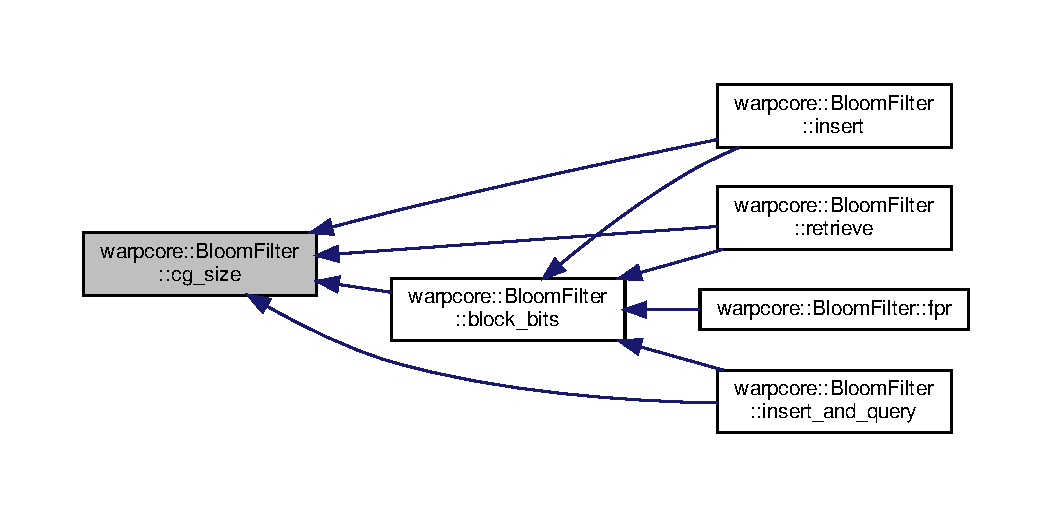
\includegraphics[width=350pt]{classwarpcore_1_1BloomFilter_a6ad2335811852ad62fc65e85416d3904_icgraph}
\end{center}
\end{figure}
\mbox{\Hypertarget{classwarpcore_1_1BloomFilter_af77c52ec3c2223cfe335a65197bed625}\label{classwarpcore_1_1BloomFilter_af77c52ec3c2223cfe335a65197bed625}} 
\index{warpcore\+::\+Bloom\+Filter@{warpcore\+::\+Bloom\+Filter}!fpr@{fpr}}
\index{fpr@{fpr}!warpcore\+::\+Bloom\+Filter@{warpcore\+::\+Bloom\+Filter}}
\subsubsection{\texorpdfstring{fpr()}{fpr()}}
{\footnotesize\ttfamily template$<$class Key , class Hasher  = defaults\+::hasher\+\_\+t$<$\+Key$>$, class Slot  = std\+::uint64\+\_\+t, index\+\_\+t C\+G\+Size = 1$>$ \\
\+\_\+\+\_\+host\+\_\+\+\_\+ double \hyperlink{classwarpcore_1_1BloomFilter}{warpcore\+::\+Bloom\+Filter}$<$ Key, Hasher, Slot, C\+G\+Size $>$\+::fpr (\begin{DoxyParamCaption}\item[{index\+\_\+type}]{n }\end{DoxyParamCaption}) const\hspace{0.3cm}{\ttfamily [inline]}, {\ttfamily [noexcept]}}



estimated false positive rate of pattern-\/blocked bloom filter 


\begin{DoxyParams}[1]{Parameters}
\mbox{\tt in}  & {\em n} & number of inserted elements \\
\hline
\end{DoxyParams}
\begin{DoxyReturn}{Returns}
false positive rate 
\end{DoxyReturn}
\begin{DoxyWarning}{Warning}
computationally expensive for large filters 
\end{DoxyWarning}
Here is the call graph for this function\+:
\nopagebreak
\begin{figure}[H]
\begin{center}
\leavevmode
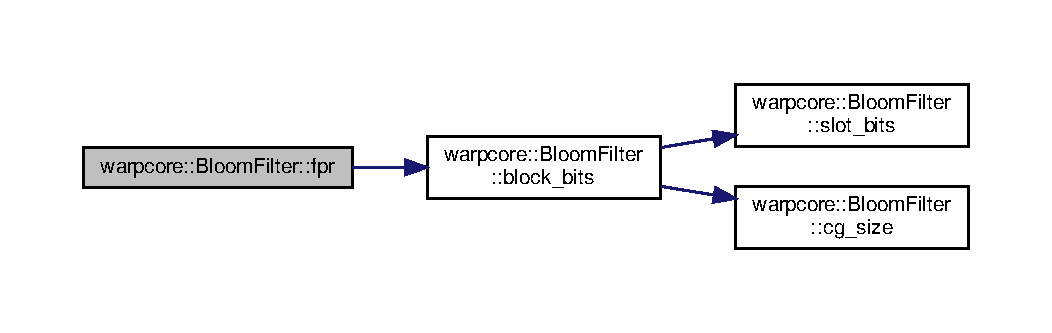
\includegraphics[width=350pt]{classwarpcore_1_1BloomFilter_af77c52ec3c2223cfe335a65197bed625_cgraph}
\end{center}
\end{figure}
\mbox{\Hypertarget{classwarpcore_1_1BloomFilter_ac9e663f21e94822fc214b75c623436f5}\label{classwarpcore_1_1BloomFilter_ac9e663f21e94822fc214b75c623436f5}} 
\index{warpcore\+::\+Bloom\+Filter@{warpcore\+::\+Bloom\+Filter}!init@{init}}
\index{init@{init}!warpcore\+::\+Bloom\+Filter@{warpcore\+::\+Bloom\+Filter}}
\subsubsection{\texorpdfstring{init()}{init()}}
{\footnotesize\ttfamily template$<$class Key , class Hasher  = defaults\+::hasher\+\_\+t$<$\+Key$>$, class Slot  = std\+::uint64\+\_\+t, index\+\_\+t C\+G\+Size = 1$>$ \\
\+\_\+\+\_\+host\+\_\+\+\_\+ void \hyperlink{classwarpcore_1_1BloomFilter}{warpcore\+::\+Bloom\+Filter}$<$ Key, Hasher, Slot, C\+G\+Size $>$\+::init (\begin{DoxyParamCaption}\item[{cuda\+Stream\+\_\+t}]{stream = {\ttfamily 0} }\end{DoxyParamCaption})\hspace{0.3cm}{\ttfamily [inline]}, {\ttfamily [noexcept]}}



re-\/initialize the hash table 


\begin{DoxyParams}[1]{Parameters}
\mbox{\tt in}  & {\em stream} & C\+U\+DA stream in which this operation is executed in \\
\hline
\end{DoxyParams}
Here is the caller graph for this function\+:
\nopagebreak
\begin{figure}[H]
\begin{center}
\leavevmode
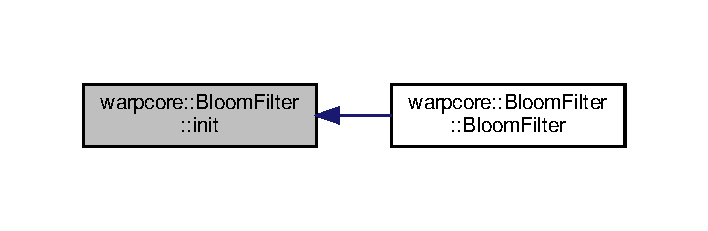
\includegraphics[width=340pt]{classwarpcore_1_1BloomFilter_ac9e663f21e94822fc214b75c623436f5_icgraph}
\end{center}
\end{figure}
\mbox{\Hypertarget{classwarpcore_1_1BloomFilter_a8567325cd30886f3daf2c615a35bb02e}\label{classwarpcore_1_1BloomFilter_a8567325cd30886f3daf2c615a35bb02e}} 
\index{warpcore\+::\+Bloom\+Filter@{warpcore\+::\+Bloom\+Filter}!insert@{insert}}
\index{insert@{insert}!warpcore\+::\+Bloom\+Filter@{warpcore\+::\+Bloom\+Filter}}
\subsubsection{\texorpdfstring{insert()}{insert()}\hspace{0.1cm}{\footnotesize\ttfamily [1/2]}}
{\footnotesize\ttfamily template$<$class Key , class Hasher  = defaults\+::hasher\+\_\+t$<$\+Key$>$, class Slot  = std\+::uint64\+\_\+t, index\+\_\+t C\+G\+Size = 1$>$ \\
\+\_\+\+\_\+device\+\_\+\+\_\+ void \hyperlink{classwarpcore_1_1BloomFilter}{warpcore\+::\+Bloom\+Filter}$<$ Key, Hasher, Slot, C\+G\+Size $>$\+::insert (\begin{DoxyParamCaption}\item[{key\+\_\+type}]{key,  }\item[{const cg\+::thread\+\_\+block\+\_\+tile$<$ \hyperlink{classwarpcore_1_1BloomFilter_a6ad2335811852ad62fc65e85416d3904}{cg\+\_\+size}()$>$ \&}]{group }\end{DoxyParamCaption})\hspace{0.3cm}{\ttfamily [inline]}, {\ttfamily [noexcept]}}



inserts a key into the bloom filter 


\begin{DoxyParams}[1]{Parameters}
\mbox{\tt in}  & {\em key} & key to insert into the bloom filter \\
\hline
\mbox{\tt in}  & {\em group} & cooperative group \\
\hline
\end{DoxyParams}
Here is the call graph for this function\+:
\nopagebreak
\begin{figure}[H]
\begin{center}
\leavevmode
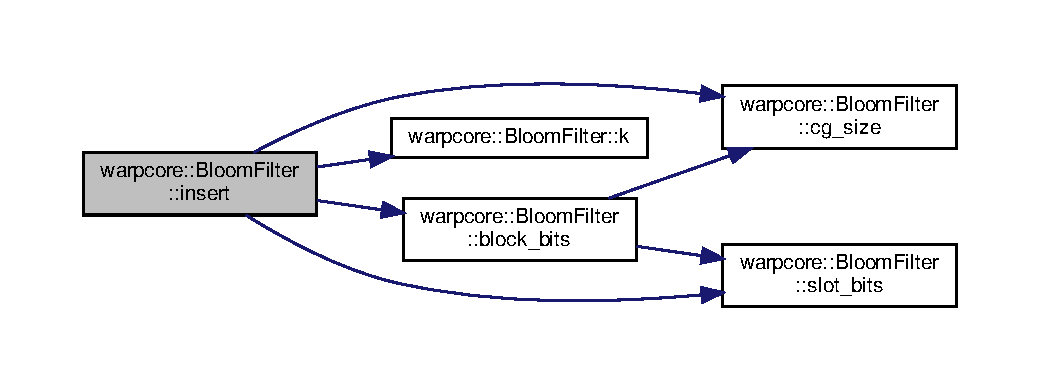
\includegraphics[width=350pt]{classwarpcore_1_1BloomFilter_a8567325cd30886f3daf2c615a35bb02e_cgraph}
\end{center}
\end{figure}
\mbox{\Hypertarget{classwarpcore_1_1BloomFilter_a462859be5ed949c82d37909b139271ee}\label{classwarpcore_1_1BloomFilter_a462859be5ed949c82d37909b139271ee}} 
\index{warpcore\+::\+Bloom\+Filter@{warpcore\+::\+Bloom\+Filter}!insert@{insert}}
\index{insert@{insert}!warpcore\+::\+Bloom\+Filter@{warpcore\+::\+Bloom\+Filter}}
\subsubsection{\texorpdfstring{insert()}{insert()}\hspace{0.1cm}{\footnotesize\ttfamily [2/2]}}
{\footnotesize\ttfamily template$<$class Key , class Hasher  = defaults\+::hasher\+\_\+t$<$\+Key$>$, class Slot  = std\+::uint64\+\_\+t, index\+\_\+t C\+G\+Size = 1$>$ \\
\+\_\+\+\_\+host\+\_\+\+\_\+ void \hyperlink{classwarpcore_1_1BloomFilter}{warpcore\+::\+Bloom\+Filter}$<$ Key, Hasher, Slot, C\+G\+Size $>$\+::insert (\begin{DoxyParamCaption}\item[{Key $\ast$}]{keys\+\_\+in,  }\item[{index\+\_\+t}]{size\+\_\+in,  }\item[{cuda\+Stream\+\_\+t}]{stream = {\ttfamily 0} }\end{DoxyParamCaption})\hspace{0.3cm}{\ttfamily [inline]}, {\ttfamily [noexcept]}}



inserts a set of keys into the bloom filter 


\begin{DoxyParams}[1]{Parameters}
\mbox{\tt in}  & {\em keys\+\_\+in} & pointer to keys to insert into the bloom filter \\
\hline
\mbox{\tt in}  & {\em size\+\_\+in} & number of keys to insert \\
\hline
\mbox{\tt in}  & {\em stream} & C\+U\+DA stream in which this operation is executed in \\
\hline
\end{DoxyParams}
Here is the call graph for this function\+:
\nopagebreak
\begin{figure}[H]
\begin{center}
\leavevmode
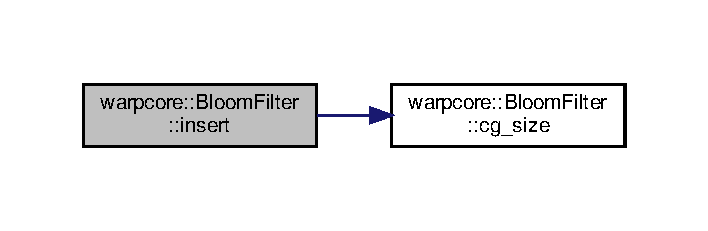
\includegraphics[width=340pt]{classwarpcore_1_1BloomFilter_a462859be5ed949c82d37909b139271ee_cgraph}
\end{center}
\end{figure}
\mbox{\Hypertarget{classwarpcore_1_1BloomFilter_a6dc903341218173f276cc855ba683ad1}\label{classwarpcore_1_1BloomFilter_a6dc903341218173f276cc855ba683ad1}} 
\index{warpcore\+::\+Bloom\+Filter@{warpcore\+::\+Bloom\+Filter}!insert\+\_\+and\+\_\+query@{insert\+\_\+and\+\_\+query}}
\index{insert\+\_\+and\+\_\+query@{insert\+\_\+and\+\_\+query}!warpcore\+::\+Bloom\+Filter@{warpcore\+::\+Bloom\+Filter}}
\subsubsection{\texorpdfstring{insert\+\_\+and\+\_\+query()}{insert\_and\_query()}}
{\footnotesize\ttfamily template$<$class Key , class Hasher  = defaults\+::hasher\+\_\+t$<$\+Key$>$, class Slot  = std\+::uint64\+\_\+t, index\+\_\+t C\+G\+Size = 1$>$ \\
template$<$index\+\_\+type C\+G\+Size\+\_\+ = cg\+\_\+size(), class  = std\+::enable\+\_\+if\+\_\+t$<$\+C\+G\+Size\+\_\+ == 1$>$$>$ \\
\+\_\+\+\_\+device\+\_\+\+\_\+ bool \hyperlink{classwarpcore_1_1BloomFilter}{warpcore\+::\+Bloom\+Filter}$<$ Key, Hasher, Slot, C\+G\+Size $>$\+::insert\+\_\+and\+\_\+query (\begin{DoxyParamCaption}\item[{key\+\_\+type}]{key,  }\item[{const cg\+::thread\+\_\+block\+\_\+tile$<$ \hyperlink{classwarpcore_1_1BloomFilter_a6ad2335811852ad62fc65e85416d3904}{cg\+\_\+size}()$>$ \&}]{group }\end{DoxyParamCaption})\hspace{0.3cm}{\ttfamily [inline]}, {\ttfamily [noexcept]}}



queries and subsequently inserts a key into the bloom filter 

\begin{DoxyNote}{Note}
can only be used when {\ttfamily C\+G\+Size==1} to prevent from race conditions 
\end{DoxyNote}

\begin{DoxyParams}[1]{Parameters}
\mbox{\tt in}  & {\em key} & key to query \\
\hline
\mbox{\tt in}  & {\em group} & cooperative group this operation is executed in \\
\hline
\mbox{\tt out}  & {\em flag} & whether the key was already inside the filter before insertion \\
\hline
\end{DoxyParams}
Here is the call graph for this function\+:
\nopagebreak
\begin{figure}[H]
\begin{center}
\leavevmode
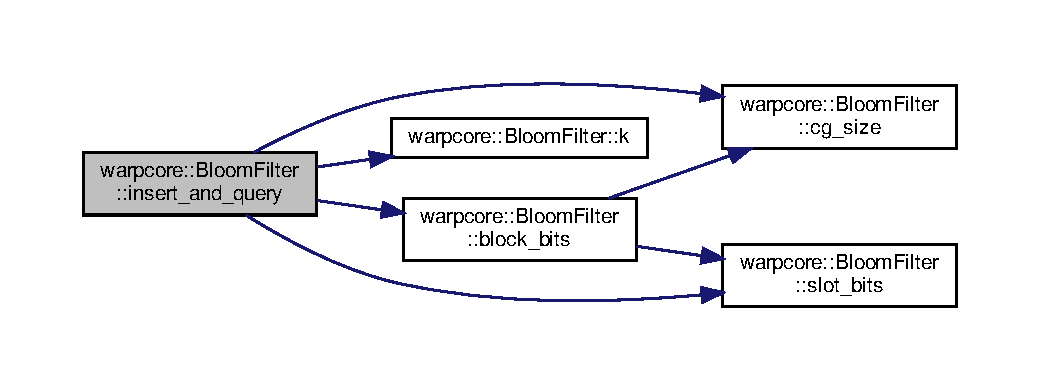
\includegraphics[width=350pt]{classwarpcore_1_1BloomFilter_a6dc903341218173f276cc855ba683ad1_cgraph}
\end{center}
\end{figure}
\mbox{\Hypertarget{classwarpcore_1_1BloomFilter_a55aaae73d8a1a8d811779fcf372f6c8c}\label{classwarpcore_1_1BloomFilter_a55aaae73d8a1a8d811779fcf372f6c8c}} 
\index{warpcore\+::\+Bloom\+Filter@{warpcore\+::\+Bloom\+Filter}!is\+\_\+copy@{is\+\_\+copy}}
\index{is\+\_\+copy@{is\+\_\+copy}!warpcore\+::\+Bloom\+Filter@{warpcore\+::\+Bloom\+Filter}}
\subsubsection{\texorpdfstring{is\+\_\+copy()}{is\_copy()}}
{\footnotesize\ttfamily template$<$class Key , class Hasher  = defaults\+::hasher\+\_\+t$<$\+Key$>$, class Slot  = std\+::uint64\+\_\+t, index\+\_\+t C\+G\+Size = 1$>$ \\
\+\_\+\+\_\+host\+\_\+\+\_\+\+\_\+\+\_\+device\+\_\+\+\_\+ bool \hyperlink{classwarpcore_1_1BloomFilter}{warpcore\+::\+Bloom\+Filter}$<$ Key, Hasher, Slot, C\+G\+Size $>$\+::is\+\_\+copy (\begin{DoxyParamCaption}{ }\end{DoxyParamCaption}) const\hspace{0.3cm}{\ttfamily [inline]}, {\ttfamily [noexcept]}}



indicates if this object is a shallow copy 

\begin{DoxyReturn}{Returns}
{\ttfamily bool} 
\end{DoxyReturn}
Here is the call graph for this function\+:
\nopagebreak
\begin{figure}[H]
\begin{center}
\leavevmode
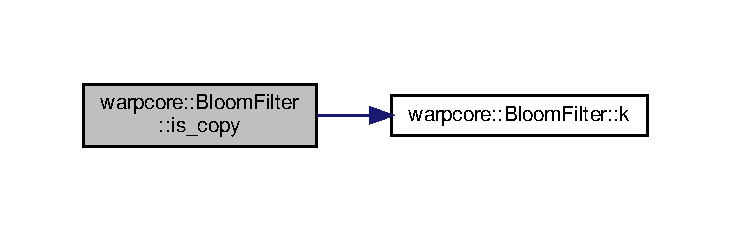
\includegraphics[width=350pt]{classwarpcore_1_1BloomFilter_a55aaae73d8a1a8d811779fcf372f6c8c_cgraph}
\end{center}
\end{figure}
\mbox{\Hypertarget{classwarpcore_1_1BloomFilter_a33c972e8a462625d6253b58bbd5585f3}\label{classwarpcore_1_1BloomFilter_a33c972e8a462625d6253b58bbd5585f3}} 
\index{warpcore\+::\+Bloom\+Filter@{warpcore\+::\+Bloom\+Filter}!k@{k}}
\index{k@{k}!warpcore\+::\+Bloom\+Filter@{warpcore\+::\+Bloom\+Filter}}
\subsubsection{\texorpdfstring{k()}{k()}}
{\footnotesize\ttfamily template$<$class Key , class Hasher  = defaults\+::hasher\+\_\+t$<$\+Key$>$, class Slot  = std\+::uint64\+\_\+t, index\+\_\+t C\+G\+Size = 1$>$ \\
\+\_\+\+\_\+host\+\_\+\+\_\+\+\_\+\+\_\+device\+\_\+\+\_\+ index\+\_\+type \hyperlink{classwarpcore_1_1BloomFilter}{warpcore\+::\+Bloom\+Filter}$<$ Key, Hasher, Slot, C\+G\+Size $>$\+::k (\begin{DoxyParamCaption}{ }\end{DoxyParamCaption}) const\hspace{0.3cm}{\ttfamily [inline]}, {\ttfamily [noexcept]}}



get number of hash functions (k) 

\begin{DoxyReturn}{Returns}
number of hash functions (k) 
\end{DoxyReturn}
Here is the caller graph for this function\+:
\nopagebreak
\begin{figure}[H]
\begin{center}
\leavevmode
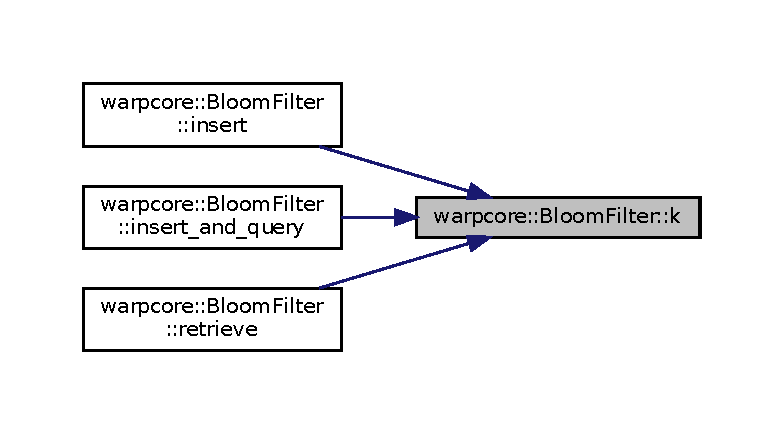
\includegraphics[width=350pt]{classwarpcore_1_1BloomFilter_a33c972e8a462625d6253b58bbd5585f3_icgraph}
\end{center}
\end{figure}
\mbox{\Hypertarget{classwarpcore_1_1BloomFilter_a54a25926cf770e834c47ad5164e91443}\label{classwarpcore_1_1BloomFilter_a54a25926cf770e834c47ad5164e91443}} 
\index{warpcore\+::\+Bloom\+Filter@{warpcore\+::\+Bloom\+Filter}!num\+\_\+bits@{num\+\_\+bits}}
\index{num\+\_\+bits@{num\+\_\+bits}!warpcore\+::\+Bloom\+Filter@{warpcore\+::\+Bloom\+Filter}}
\subsubsection{\texorpdfstring{num\+\_\+bits()}{num\_bits()}}
{\footnotesize\ttfamily template$<$class Key , class Hasher  = defaults\+::hasher\+\_\+t$<$\+Key$>$, class Slot  = std\+::uint64\+\_\+t, index\+\_\+t C\+G\+Size = 1$>$ \\
\+\_\+\+\_\+host\+\_\+\+\_\+\+\_\+\+\_\+device\+\_\+\+\_\+ index\+\_\+type \hyperlink{classwarpcore_1_1BloomFilter}{warpcore\+::\+Bloom\+Filter}$<$ Key, Hasher, Slot, C\+G\+Size $>$\+::num\+\_\+bits (\begin{DoxyParamCaption}{ }\end{DoxyParamCaption}) const\hspace{0.3cm}{\ttfamily [inline]}, {\ttfamily [noexcept]}}



get number of bits (m) 

\begin{DoxyReturn}{Returns}
number of bits (m) 
\end{DoxyReturn}
\mbox{\Hypertarget{classwarpcore_1_1BloomFilter_a10fcbb540441eff40a1d0fccd1b992bd}\label{classwarpcore_1_1BloomFilter_a10fcbb540441eff40a1d0fccd1b992bd}} 
\index{warpcore\+::\+Bloom\+Filter@{warpcore\+::\+Bloom\+Filter}!num\+\_\+blocks@{num\+\_\+blocks}}
\index{num\+\_\+blocks@{num\+\_\+blocks}!warpcore\+::\+Bloom\+Filter@{warpcore\+::\+Bloom\+Filter}}
\subsubsection{\texorpdfstring{num\+\_\+blocks()}{num\_blocks()}}
{\footnotesize\ttfamily template$<$class Key , class Hasher  = defaults\+::hasher\+\_\+t$<$\+Key$>$, class Slot  = std\+::uint64\+\_\+t, index\+\_\+t C\+G\+Size = 1$>$ \\
\+\_\+\+\_\+host\+\_\+\+\_\+\+\_\+\+\_\+device\+\_\+\+\_\+ index\+\_\+type \hyperlink{classwarpcore_1_1BloomFilter}{warpcore\+::\+Bloom\+Filter}$<$ Key, Hasher, Slot, C\+G\+Size $>$\+::num\+\_\+blocks (\begin{DoxyParamCaption}{ }\end{DoxyParamCaption}) const\hspace{0.3cm}{\ttfamily [inline]}, {\ttfamily [noexcept]}}



get number of blocks 

\begin{DoxyReturn}{Returns}
number of blocks 
\end{DoxyReturn}
\mbox{\Hypertarget{classwarpcore_1_1BloomFilter_a1ab7ecd7bcc3f6321a252f94d63965eb}\label{classwarpcore_1_1BloomFilter_a1ab7ecd7bcc3f6321a252f94d63965eb}} 
\index{warpcore\+::\+Bloom\+Filter@{warpcore\+::\+Bloom\+Filter}!num\+\_\+slots@{num\+\_\+slots}}
\index{num\+\_\+slots@{num\+\_\+slots}!warpcore\+::\+Bloom\+Filter@{warpcore\+::\+Bloom\+Filter}}
\subsubsection{\texorpdfstring{num\+\_\+slots()}{num\_slots()}}
{\footnotesize\ttfamily template$<$class Key , class Hasher  = defaults\+::hasher\+\_\+t$<$\+Key$>$, class Slot  = std\+::uint64\+\_\+t, index\+\_\+t C\+G\+Size = 1$>$ \\
\+\_\+\+\_\+host\+\_\+\+\_\+\+\_\+\+\_\+device\+\_\+\+\_\+ index\+\_\+type \hyperlink{classwarpcore_1_1BloomFilter}{warpcore\+::\+Bloom\+Filter}$<$ Key, Hasher, Slot, C\+G\+Size $>$\+::num\+\_\+slots (\begin{DoxyParamCaption}{ }\end{DoxyParamCaption}) const\hspace{0.3cm}{\ttfamily [inline]}, {\ttfamily [noexcept]}}



get number of slots 

\begin{DoxyReturn}{Returns}
number of slots 
\end{DoxyReturn}
\mbox{\Hypertarget{classwarpcore_1_1BloomFilter_a47ffce0fc70aa6bd7a0ed4b837fec1bd}\label{classwarpcore_1_1BloomFilter_a47ffce0fc70aa6bd7a0ed4b837fec1bd}} 
\index{warpcore\+::\+Bloom\+Filter@{warpcore\+::\+Bloom\+Filter}!retrieve@{retrieve}}
\index{retrieve@{retrieve}!warpcore\+::\+Bloom\+Filter@{warpcore\+::\+Bloom\+Filter}}
\subsubsection{\texorpdfstring{retrieve()}{retrieve()}\hspace{0.1cm}{\footnotesize\ttfamily [1/2]}}
{\footnotesize\ttfamily template$<$class Key , class Hasher  = defaults\+::hasher\+\_\+t$<$\+Key$>$, class Slot  = std\+::uint64\+\_\+t, index\+\_\+t C\+G\+Size = 1$>$ \\
\+\_\+\+\_\+device\+\_\+\+\_\+ bool \hyperlink{classwarpcore_1_1BloomFilter}{warpcore\+::\+Bloom\+Filter}$<$ Key, Hasher, Slot, C\+G\+Size $>$\+::retrieve (\begin{DoxyParamCaption}\item[{key\+\_\+type}]{key,  }\item[{const cg\+::thread\+\_\+block\+\_\+tile$<$ \hyperlink{classwarpcore_1_1BloomFilter_a6ad2335811852ad62fc65e85416d3904}{cg\+\_\+size}()$>$ \&}]{group }\end{DoxyParamCaption}) const\hspace{0.3cm}{\ttfamily [inline]}, {\ttfamily [noexcept]}}



retrieve a key 


\begin{DoxyParams}[1]{Parameters}
\mbox{\tt in}  & {\em key} & key to query \\
\hline
\mbox{\tt in}  & {\em group} & cooperative group \\
\hline
\end{DoxyParams}
\begin{DoxyReturn}{Returns}
whether the key is already inside the filter or not 
\end{DoxyReturn}
Here is the call graph for this function\+:
\nopagebreak
\begin{figure}[H]
\begin{center}
\leavevmode
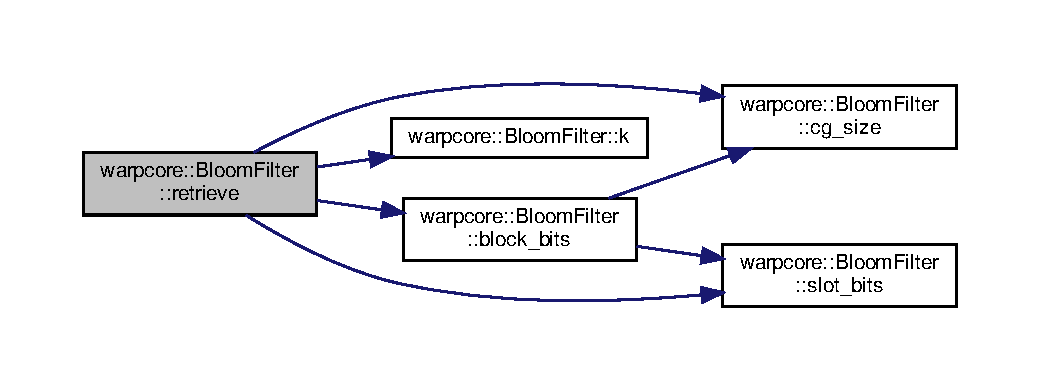
\includegraphics[width=350pt]{classwarpcore_1_1BloomFilter_a47ffce0fc70aa6bd7a0ed4b837fec1bd_cgraph}
\end{center}
\end{figure}
\mbox{\Hypertarget{classwarpcore_1_1BloomFilter_a38025d88272e7de413210efe745aa279}\label{classwarpcore_1_1BloomFilter_a38025d88272e7de413210efe745aa279}} 
\index{warpcore\+::\+Bloom\+Filter@{warpcore\+::\+Bloom\+Filter}!retrieve@{retrieve}}
\index{retrieve@{retrieve}!warpcore\+::\+Bloom\+Filter@{warpcore\+::\+Bloom\+Filter}}
\subsubsection{\texorpdfstring{retrieve()}{retrieve()}\hspace{0.1cm}{\footnotesize\ttfamily [2/2]}}
{\footnotesize\ttfamily template$<$class Key , class Hasher  = defaults\+::hasher\+\_\+t$<$\+Key$>$, class Slot  = std\+::uint64\+\_\+t, index\+\_\+t C\+G\+Size = 1$>$ \\
\+\_\+\+\_\+host\+\_\+\+\_\+ void \hyperlink{classwarpcore_1_1BloomFilter}{warpcore\+::\+Bloom\+Filter}$<$ Key, Hasher, Slot, C\+G\+Size $>$\+::retrieve (\begin{DoxyParamCaption}\item[{key\+\_\+type $\ast$}]{keys\+\_\+in,  }\item[{index\+\_\+type}]{size\+\_\+in,  }\item[{bool $\ast$}]{flags\+\_\+out,  }\item[{cuda\+Stream\+\_\+t}]{stream = {\ttfamily 0} }\end{DoxyParamCaption}) const\hspace{0.3cm}{\ttfamily [inline]}, {\ttfamily [noexcept]}}



retrieve a set of keys 


\begin{DoxyParams}[1]{Parameters}
\mbox{\tt in}  & {\em keys\+\_\+in} & pointer to keys \\
\hline
\mbox{\tt in}  & {\em size\+\_\+in} & number of keys \\
\hline
\mbox{\tt out}  & {\em flags\+\_\+out} & result per key \textquotesingle{} \\
\hline
\mbox{\tt in}  & {\em stream} & C\+U\+DA stream in which this operation is executed in \\
\hline
\end{DoxyParams}
Here is the call graph for this function\+:
\nopagebreak
\begin{figure}[H]
\begin{center}
\leavevmode
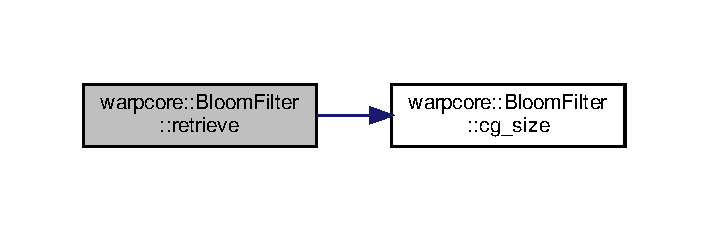
\includegraphics[width=340pt]{classwarpcore_1_1BloomFilter_a38025d88272e7de413210efe745aa279_cgraph}
\end{center}
\end{figure}
\mbox{\Hypertarget{classwarpcore_1_1BloomFilter_a8dca50765c601cca8d85621fa8488ecc}\label{classwarpcore_1_1BloomFilter_a8dca50765c601cca8d85621fa8488ecc}} 
\index{warpcore\+::\+Bloom\+Filter@{warpcore\+::\+Bloom\+Filter}!slot\+\_\+bits@{slot\+\_\+bits}}
\index{slot\+\_\+bits@{slot\+\_\+bits}!warpcore\+::\+Bloom\+Filter@{warpcore\+::\+Bloom\+Filter}}
\subsubsection{\texorpdfstring{slot\+\_\+bits()}{slot\_bits()}}
{\footnotesize\ttfamily template$<$class Key , class Hasher  = defaults\+::hasher\+\_\+t$<$\+Key$>$, class Slot  = std\+::uint64\+\_\+t, index\+\_\+t C\+G\+Size = 1$>$ \\
static \+\_\+\+\_\+host\+\_\+\+\_\+\+\_\+\+\_\+device\+\_\+\+\_\+ constexpr index\+\_\+type \hyperlink{classwarpcore_1_1BloomFilter}{warpcore\+::\+Bloom\+Filter}$<$ Key, Hasher, Slot, C\+G\+Size $>$\+::slot\+\_\+bits (\begin{DoxyParamCaption}{ }\end{DoxyParamCaption})\hspace{0.3cm}{\ttfamily [inline]}, {\ttfamily [static]}, {\ttfamily [noexcept]}}



get bits per slot 

\begin{DoxyReturn}{Returns}
number of bits 
\end{DoxyReturn}
Here is the caller graph for this function\+:
\nopagebreak
\begin{figure}[H]
\begin{center}
\leavevmode
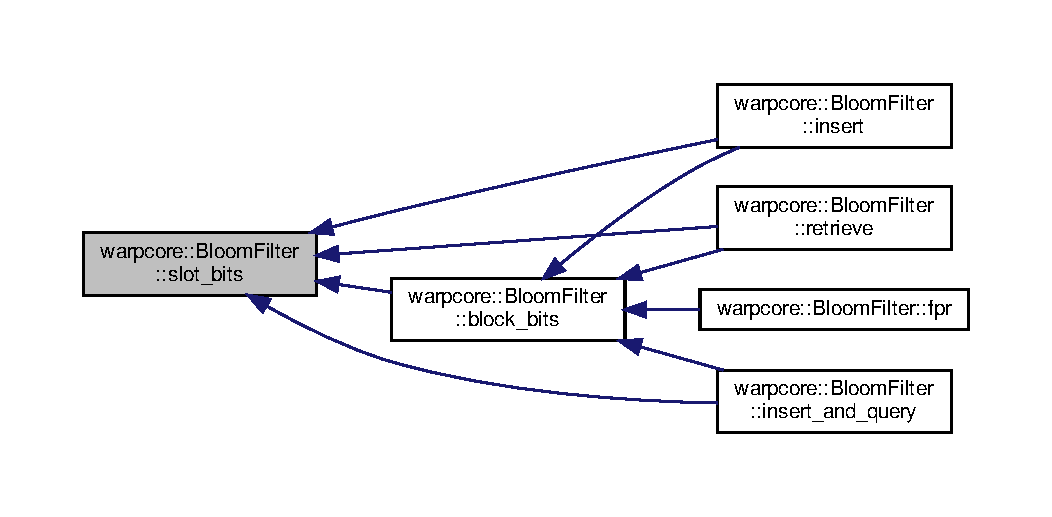
\includegraphics[width=350pt]{classwarpcore_1_1BloomFilter_a8dca50765c601cca8d85621fa8488ecc_icgraph}
\end{center}
\end{figure}

\hypertarget{classwarpcore_1_1CountingHashTable}{}\doxysection{warpcore\+::Counting\+Hash\+Table$<$ Key, Value, Empty\+Key, Tombstone\+Key, Probing\+Scheme, Table\+Storage, Temp\+Memory\+Bytes $>$ Class Template Reference}
\label{classwarpcore_1_1CountingHashTable}\index{warpcore::CountingHashTable$<$ Key, Value, EmptyKey, TombstoneKey, ProbingScheme, TableStorage, TempMemoryBytes $>$@{warpcore::CountingHashTable$<$ Key, Value, EmptyKey, TombstoneKey, ProbingScheme, TableStorage, TempMemoryBytes $>$}}


counting hash table  


\doxysubsection*{Public Types}
\begin{DoxyCompactItemize}
\item 
\mbox{\Hypertarget{classwarpcore_1_1CountingHashTable_aa0a20d833b8366c642acc976c811a415}\label{classwarpcore_1_1CountingHashTable_aa0a20d833b8366c642acc976c811a415}} 
using {\bfseries key\+\_\+type} = typename base\+\_\+type\+::key\+\_\+type
\item 
\mbox{\Hypertarget{classwarpcore_1_1CountingHashTable_a54cb72d239d8f22878b3e9b8f3747f18}\label{classwarpcore_1_1CountingHashTable_a54cb72d239d8f22878b3e9b8f3747f18}} 
using {\bfseries value\+\_\+type} = typename base\+\_\+type\+::value\+\_\+type
\item 
\mbox{\Hypertarget{classwarpcore_1_1CountingHashTable_ab52c5d70cbaaf14be48225373435b2b4}\label{classwarpcore_1_1CountingHashTable_ab52c5d70cbaaf14be48225373435b2b4}} 
using {\bfseries index\+\_\+type} = typename base\+\_\+type\+::index\+\_\+type
\item 
\mbox{\Hypertarget{classwarpcore_1_1CountingHashTable_a0c86dbcd344a2b465275507f2910ce4e}\label{classwarpcore_1_1CountingHashTable_a0c86dbcd344a2b465275507f2910ce4e}} 
using {\bfseries status\+\_\+type} = typename \mbox{\hyperlink{classwarpcore_1_1Status}{base\+\_\+type\+::status\+\_\+type}}
\end{DoxyCompactItemize}
\doxysubsection*{Public Member Functions}
\begin{DoxyCompactItemize}
\item 
\+\_\+\+\_\+host\+\_\+\+\_\+ \mbox{\hyperlink{classwarpcore_1_1CountingHashTable_a68946e67712e7b2afb95ddb7169a26fd}{Counting\+Hash\+Table}} (index\+\_\+type min\+\_\+capacity, key\+\_\+type \mbox{\hyperlink{classwarpcore_1_1CountingHashTable_a404f39442f096f294cd879b0710e5416}{seed}}=defaults\+::seed$<$ key\+\_\+type $>$(), value\+\_\+type max\+\_\+count=std\+::numeric\+\_\+limits$<$ value\+\_\+type $>$\+::max(), bool no\+\_\+init=false) noexcept
\begin{DoxyCompactList}\small\item\em constructor \end{DoxyCompactList}\item 
\+\_\+\+\_\+host\+\_\+\+\_\+\+\_\+\+\_\+device\+\_\+\+\_\+ \mbox{\hyperlink{classwarpcore_1_1CountingHashTable_afba99fa2513c3ca3c7708ac718d2b0fc}{Counting\+Hash\+Table}} (const \mbox{\hyperlink{classwarpcore_1_1CountingHashTable}{Counting\+Hash\+Table}} \&o) noexcept
\begin{DoxyCompactList}\small\item\em copy-\/constructor (shallow) \end{DoxyCompactList}\item 
\+\_\+\+\_\+host\+\_\+\+\_\+ \mbox{\hyperlink{classwarpcore_1_1CountingHashTable_ab1c1ea195d10fbbdb6a70e5f3bf96623}{Counting\+Hash\+Table}} (\mbox{\hyperlink{classwarpcore_1_1CountingHashTable}{Counting\+Hash\+Table}} \&\&o) noexcept
\begin{DoxyCompactList}\small\item\em move-\/constructor \end{DoxyCompactList}\item 
\+\_\+\+\_\+host\+\_\+\+\_\+ void \mbox{\hyperlink{classwarpcore_1_1CountingHashTable_acb401fb2d38c59e086a1bedf68d4815f}{init}} (const key\+\_\+type \mbox{\hyperlink{classwarpcore_1_1CountingHashTable_a404f39442f096f294cd879b0710e5416}{seed}}, const cuda\+Stream\+\_\+t stream=0) noexcept
\begin{DoxyCompactList}\small\item\em (re)initialize the hash table \end{DoxyCompactList}\item 
\+\_\+\+\_\+host\+\_\+\+\_\+ void \mbox{\hyperlink{classwarpcore_1_1CountingHashTable_a8b7a93faf9c5746c2665b4b775f9de88}{init}} (const cuda\+Stream\+\_\+t stream=0) noexcept
\begin{DoxyCompactList}\small\item\em (re)initialize the hash table \end{DoxyCompactList}\item 
\+\_\+\+\_\+device\+\_\+\+\_\+ status\+\_\+type \mbox{\hyperlink{classwarpcore_1_1CountingHashTable_a2cad25fea134d836cf1b75f67d6b38ac}{insert}} (key\+\_\+type key\+\_\+in, const cg\+::thread\+\_\+block\+\_\+tile$<$ \mbox{\hyperlink{classwarpcore_1_1CountingHashTable_a5efe6f4060321596322a99a28fcaef93}{cg\+\_\+size}}()$>$ \&group, index\+\_\+type probing\+\_\+length=defaults\+::probing\+\_\+length()) noexcept
\begin{DoxyCompactList}\small\item\em inserts a key into the hash table \end{DoxyCompactList}\item 
{\footnotesize template$<$class Status\+Handler  = defaults\+::status\+\_\+handler\+\_\+t$>$ }\\\+\_\+\+\_\+host\+\_\+\+\_\+ void \mbox{\hyperlink{classwarpcore_1_1CountingHashTable_a36d896f2f66465925ea21a9f01bb12f3}{insert}} (key\+\_\+type $\ast$keys\+\_\+in, index\+\_\+type num\+\_\+in, cuda\+Stream\+\_\+t stream=0, index\+\_\+type probing\+\_\+length=defaults\+::probing\+\_\+length(), typename Status\+Handler\+::base\+\_\+type $\ast$status\+\_\+out=nullptr) noexcept
\begin{DoxyCompactList}\small\item\em insert a set of keys into the hash table \end{DoxyCompactList}\item 
\+\_\+\+\_\+device\+\_\+\+\_\+ status\+\_\+type \mbox{\hyperlink{classwarpcore_1_1CountingHashTable_ab156b6726ca60e401fae990274b40cfc}{retrieve}} (key\+\_\+type key\+\_\+in, value\+\_\+type \&value\+\_\+out, const cg\+::thread\+\_\+block\+\_\+tile$<$ \mbox{\hyperlink{classwarpcore_1_1CountingHashTable_a5efe6f4060321596322a99a28fcaef93}{cg\+\_\+size}}()$>$ \&group, index\+\_\+type probing\+\_\+length=defaults\+::probing\+\_\+length()) const noexcept
\begin{DoxyCompactList}\small\item\em retrieves a key from the hash table \end{DoxyCompactList}\item 
{\footnotesize template$<$class Status\+Handler  = defaults\+::status\+\_\+handler\+\_\+t$>$ }\\\+\_\+\+\_\+host\+\_\+\+\_\+ void \mbox{\hyperlink{classwarpcore_1_1CountingHashTable_a9abe12f3b4110a53e0cfc89a480a798f}{retrieve}} (key\+\_\+type $\ast$keys\+\_\+in, index\+\_\+type num\+\_\+in, value\+\_\+type $\ast$values\+\_\+out, cuda\+Stream\+\_\+t stream=0, index\+\_\+type probing\+\_\+length=defaults\+::probing\+\_\+length(), typename Status\+Handler\+::base\+\_\+type $\ast$status\+\_\+out=nullptr) const noexcept
\begin{DoxyCompactList}\small\item\em retrieve a set of keys from the hash table \end{DoxyCompactList}\item 
\+\_\+\+\_\+host\+\_\+\+\_\+ void \mbox{\hyperlink{classwarpcore_1_1CountingHashTable_aade49f5de5f2144d57cdcfe8b7ad6663}{retrieve\+\_\+all}} (key\+\_\+type $\ast$keys\+\_\+out, value\+\_\+type $\ast$values\+\_\+out, index\+\_\+t \&num\+\_\+out, cuda\+Stream\+\_\+t stream=0) const noexcept
\begin{DoxyCompactList}\small\item\em retrieves all elements from the hash table \end{DoxyCompactList}\item 
\+\_\+\+\_\+device\+\_\+\+\_\+ status\+\_\+type \mbox{\hyperlink{classwarpcore_1_1CountingHashTable_aee43cc21c75f1ad37e79604afa034363}{erase}} (key\+\_\+type key\+\_\+in, const cg\+::thread\+\_\+block\+\_\+tile$<$ \mbox{\hyperlink{classwarpcore_1_1CountingHashTable_a5efe6f4060321596322a99a28fcaef93}{cg\+\_\+size}}()$>$ \&group, index\+\_\+type probing\+\_\+length=defaults\+::probing\+\_\+length()) noexcept
\begin{DoxyCompactList}\small\item\em erases a key from the hash table \end{DoxyCompactList}\item 
{\footnotesize template$<$class Status\+Handler  = defaults\+::status\+\_\+handler\+\_\+t$>$ }\\\+\_\+\+\_\+host\+\_\+\+\_\+ void \mbox{\hyperlink{classwarpcore_1_1CountingHashTable_ac43612ae6bae1c2b01c3b2af63d7a652}{erase}} (key\+\_\+type $\ast$keys\+\_\+in, index\+\_\+type num\+\_\+in, cuda\+Stream\+\_\+t stream=0, index\+\_\+type probing\+\_\+length=defaults\+::probing\+\_\+length(), typename Status\+Handler\+::base\+\_\+type $\ast$status\+\_\+out=nullptr) noexcept
\begin{DoxyCompactList}\small\item\em erases a set of keys from the hash table \end{DoxyCompactList}\item 
{\footnotesize template$<$class Func $>$ }\\\+\_\+\+\_\+host\+\_\+\+\_\+ void \mbox{\hyperlink{classwarpcore_1_1CountingHashTable_aea11af31c41fe5d7369b42f2b74d276a}{for\+\_\+each}} (Func f, cuda\+Stream\+\_\+t stream=0, index\+\_\+type smem\+\_\+bytes=0) const noexcept
\begin{DoxyCompactList}\small\item\em applies a funtion on all key value pairs inside the table \end{DoxyCompactList}\item 
\+\_\+\+\_\+host\+\_\+\+\_\+ index\+\_\+type \mbox{\hyperlink{classwarpcore_1_1CountingHashTable_aa331f755c38f5b073ed7e58e3ad59777}{size}} (cuda\+Stream\+\_\+t stream=0) const noexcept
\begin{DoxyCompactList}\small\item\em number of key/value pairs stored inside the hash table \end{DoxyCompactList}\item 
\+\_\+\+\_\+host\+\_\+\+\_\+ float \mbox{\hyperlink{classwarpcore_1_1CountingHashTable_ad4a829b15a3add41133437c17ab6bf67}{load\+\_\+factor}} (cuda\+Stream\+\_\+t stream=0) const noexcept
\begin{DoxyCompactList}\small\item\em current load factor of the hash table \end{DoxyCompactList}\item 
\+\_\+\+\_\+host\+\_\+\+\_\+ float \mbox{\hyperlink{classwarpcore_1_1CountingHashTable_aa7b5b49d50edc280ce007cf92abdc4ae}{storage\+\_\+density}} (cuda\+Stream\+\_\+t stream=0) const noexcept
\begin{DoxyCompactList}\small\item\em current storage density of the hash table \end{DoxyCompactList}\item 
\+\_\+\+\_\+host\+\_\+\+\_\+\+\_\+\+\_\+device\+\_\+\+\_\+ index\+\_\+type \mbox{\hyperlink{classwarpcore_1_1CountingHashTable_a05cdc2ffc3c11c2b10d90b3d8812e96d}{capacity}} () const noexcept
\begin{DoxyCompactList}\small\item\em get the capacity of the hash table \end{DoxyCompactList}\item 
\+\_\+\+\_\+host\+\_\+\+\_\+ status\+\_\+type \mbox{\hyperlink{classwarpcore_1_1CountingHashTable_ae9e388f29dae1952c2da7fed32415e35}{peek\+\_\+status}} (cuda\+Stream\+\_\+t stream=0) const noexcept
\begin{DoxyCompactList}\small\item\em get the status of the hash table \end{DoxyCompactList}\item 
\+\_\+\+\_\+host\+\_\+\+\_\+ status\+\_\+type \mbox{\hyperlink{classwarpcore_1_1CountingHashTable_a9313aefeadf39f1c0512f131859922ab}{pop\+\_\+status}} (cuda\+Stream\+\_\+t stream=0) noexcept
\begin{DoxyCompactList}\small\item\em get and reset the status of the hash table \end{DoxyCompactList}\item 
\+\_\+\+\_\+host\+\_\+\+\_\+\+\_\+\+\_\+device\+\_\+\+\_\+ key\+\_\+type \mbox{\hyperlink{classwarpcore_1_1CountingHashTable_a404f39442f096f294cd879b0710e5416}{seed}} () const noexcept
\begin{DoxyCompactList}\small\item\em get random seed \end{DoxyCompactList}\item 
\+\_\+\+\_\+host\+\_\+\+\_\+\+\_\+\+\_\+device\+\_\+\+\_\+ bool \mbox{\hyperlink{classwarpcore_1_1CountingHashTable_abd203ab693aa931917013e11c23d444c}{is\+\_\+copy}} () const noexcept
\begin{DoxyCompactList}\small\item\em indicates if this object is a shallow copy \end{DoxyCompactList}\end{DoxyCompactItemize}
\doxysubsection*{Static Public Member Functions}
\begin{DoxyCompactItemize}
\item 
static constexpr \+\_\+\+\_\+host\+\_\+\+\_\+\+\_\+\+\_\+device\+\_\+\+\_\+ key\+\_\+type \mbox{\hyperlink{classwarpcore_1_1CountingHashTable_a09c6eebe2c230885b14a6c7b97b30f65}{empty\+\_\+key}} () noexcept
\begin{DoxyCompactList}\small\item\em get empty key \end{DoxyCompactList}\item 
static constexpr \+\_\+\+\_\+host\+\_\+\+\_\+\+\_\+\+\_\+device\+\_\+\+\_\+ key\+\_\+type \mbox{\hyperlink{classwarpcore_1_1CountingHashTable_a742dcef5845153aacbf6d8790a5f0fac}{tombstone\+\_\+key}} () noexcept
\begin{DoxyCompactList}\small\item\em get tombstone key \end{DoxyCompactList}\item 
static constexpr \+\_\+\+\_\+host\+\_\+\+\_\+\+\_\+\+\_\+device\+\_\+\+\_\+ index\+\_\+type \mbox{\hyperlink{classwarpcore_1_1CountingHashTable_a5efe6f4060321596322a99a28fcaef93}{cg\+\_\+size}} () noexcept
\begin{DoxyCompactList}\small\item\em get cooperative group size \end{DoxyCompactList}\item 
static constexpr \+\_\+\+\_\+host\+\_\+\+\_\+\+\_\+\+\_\+device\+\_\+\+\_\+ bool \mbox{\hyperlink{classwarpcore_1_1CountingHashTable_a7cf82f559b57bed446328aab53ffcdd2}{is\+\_\+empty\+\_\+key}} (key\+\_\+type key) noexcept
\begin{DoxyCompactList}\small\item\em checks if {\ttfamily key} is equal to {\ttfamily Empty\+Key} \end{DoxyCompactList}\item 
static constexpr \+\_\+\+\_\+host\+\_\+\+\_\+\+\_\+\+\_\+device\+\_\+\+\_\+ bool \mbox{\hyperlink{classwarpcore_1_1CountingHashTable_ad4faa63cd0e6613135c12733c2d9fb6f}{is\+\_\+tombstone\+\_\+key}} (key\+\_\+type key) noexcept
\begin{DoxyCompactList}\small\item\em checks if {\ttfamily key} is equal to {\ttfamily Tombstone\+Key} \end{DoxyCompactList}\item 
static constexpr \+\_\+\+\_\+host\+\_\+\+\_\+\+\_\+\+\_\+device\+\_\+\+\_\+ bool \mbox{\hyperlink{classwarpcore_1_1CountingHashTable_a28bd96a747e0acd2f0136d74a44612d4}{is\+\_\+valid\+\_\+key}} (key\+\_\+type key) noexcept
\begin{DoxyCompactList}\small\item\em checks if {\ttfamily key} is equal to {\ttfamily }(Empty\+Key$\vert$$\vert$\+Tombstone\+Key) \end{DoxyCompactList}\end{DoxyCompactItemize}


\doxysubsection{Detailed Description}
\subsubsection*{template$<$class Key, class Value = index\+\_\+t, Key Empty\+Key = defaults\+::empty\+\_\+key$<$\+Key$>$(), Key Tombstone\+Key = defaults\+::tombstone\+\_\+key$<$\+Key$>$(), class Probing\+Scheme = defaults\+::probing\+\_\+scheme\+\_\+t$<$\+Key, 4$>$, class Table\+Storage = defaults\+::table\+\_\+storage\+\_\+t$<$\+Key, Value$>$, index\+\_\+t Temp\+Memory\+Bytes = defaults\+::temp\+\_\+memory\+\_\+bytes()$>$\newline
class warpcore\+::\+Counting\+Hash\+Table$<$ Key, Value, Empty\+Key, Tombstone\+Key, Probing\+Scheme, Table\+Storage, Temp\+Memory\+Bytes $>$}

counting hash table 


\begin{DoxyTemplParams}{Template Parameters}
{\em Key} & key type ({\ttfamily std\+::uint32\+\_\+t} or {\ttfamily std\+::uint64\+\_\+t}) \\
\hline
{\em Value} & value type \\
\hline
{\em Empty\+Key} & key which represents an empty slot \\
\hline
{\em Tombstone\+Key} & key which represents an erased slot \\
\hline
{\em Probing\+Scheme} & probing scheme from {\ttfamily \mbox{\hyperlink{namespacewarpcore_1_1probing__schemes}{warpcore\+::probing\+\_\+schemes}}} \\
\hline
{\em Table\+Storage} & internal storage class {\ttfamily \mbox{\hyperlink{namespacewarpcore_1_1storage_1_1key__value}{warpcore\+::storage\+::key\+\_\+value}}} \\
\hline
{\em Temp\+Memory\+Bytes} & size of temporary storage (typically a few kB) \\
\hline
\end{DoxyTemplParams}


\doxysubsection{Constructor \& Destructor Documentation}
\mbox{\Hypertarget{classwarpcore_1_1CountingHashTable_a68946e67712e7b2afb95ddb7169a26fd}\label{classwarpcore_1_1CountingHashTable_a68946e67712e7b2afb95ddb7169a26fd}} 
\index{warpcore::CountingHashTable$<$ Key, Value, EmptyKey, TombstoneKey, ProbingScheme, TableStorage, TempMemoryBytes $>$@{warpcore::CountingHashTable$<$ Key, Value, EmptyKey, TombstoneKey, ProbingScheme, TableStorage, TempMemoryBytes $>$}!CountingHashTable@{CountingHashTable}}
\index{CountingHashTable@{CountingHashTable}!warpcore::CountingHashTable$<$ Key, Value, EmptyKey, TombstoneKey, ProbingScheme, TableStorage, TempMemoryBytes $>$@{warpcore::CountingHashTable$<$ Key, Value, EmptyKey, TombstoneKey, ProbingScheme, TableStorage, TempMemoryBytes $>$}}
\doxysubsubsection{\texorpdfstring{CountingHashTable()}{CountingHashTable()}\hspace{0.1cm}{\footnotesize\ttfamily [1/3]}}
{\footnotesize\ttfamily template$<$class Key , class Value  = index\+\_\+t, Key Empty\+Key = defaults\+::empty\+\_\+key$<$\+Key$>$(), Key Tombstone\+Key = defaults\+::tombstone\+\_\+key$<$\+Key$>$(), class Probing\+Scheme  = defaults\+::probing\+\_\+scheme\+\_\+t$<$\+Key, 4$>$, class Table\+Storage  = defaults\+::table\+\_\+storage\+\_\+t$<$\+Key, Value$>$, index\+\_\+t Temp\+Memory\+Bytes = defaults\+::temp\+\_\+memory\+\_\+bytes()$>$ \\
\+\_\+\+\_\+host\+\_\+\+\_\+ \mbox{\hyperlink{classwarpcore_1_1CountingHashTable}{warpcore\+::\+Counting\+Hash\+Table}}$<$ Key, Value, Empty\+Key, Tombstone\+Key, Probing\+Scheme, Table\+Storage, Temp\+Memory\+Bytes $>$\+::\mbox{\hyperlink{classwarpcore_1_1CountingHashTable}{Counting\+Hash\+Table}} (\begin{DoxyParamCaption}\item[{index\+\_\+type}]{min\+\_\+capacity,  }\item[{key\+\_\+type}]{seed = {\ttfamily defaults\+:\+:seed$<$key\+\_\+type$>$()},  }\item[{value\+\_\+type}]{max\+\_\+count = {\ttfamily std\+:\+:numeric\+\_\+limits$<$value\+\_\+type$>$\+:\+:max()},  }\item[{bool}]{no\+\_\+init = {\ttfamily false} }\end{DoxyParamCaption})\hspace{0.3cm}{\ttfamily [inline]}, {\ttfamily [explicit]}, {\ttfamily [noexcept]}}



constructor 


\begin{DoxyParams}[1]{Parameters}
\mbox{\texttt{ in}}  & {\em min\+\_\+capacity} & minimum number of slots in the hash table \\
\hline
\mbox{\texttt{ in}}  & {\em seed} & random seed \\
\hline
\mbox{\texttt{ in}}  & {\em max\+\_\+count} & count after which to stop counting new occurrences \\
\hline
\mbox{\texttt{ in}}  & {\em no\+\_\+init} & whether to initialize the table at construction or not \\
\hline
\end{DoxyParams}
Here is the call graph for this function\+:
\nopagebreak
\begin{figure}[H]
\begin{center}
\leavevmode
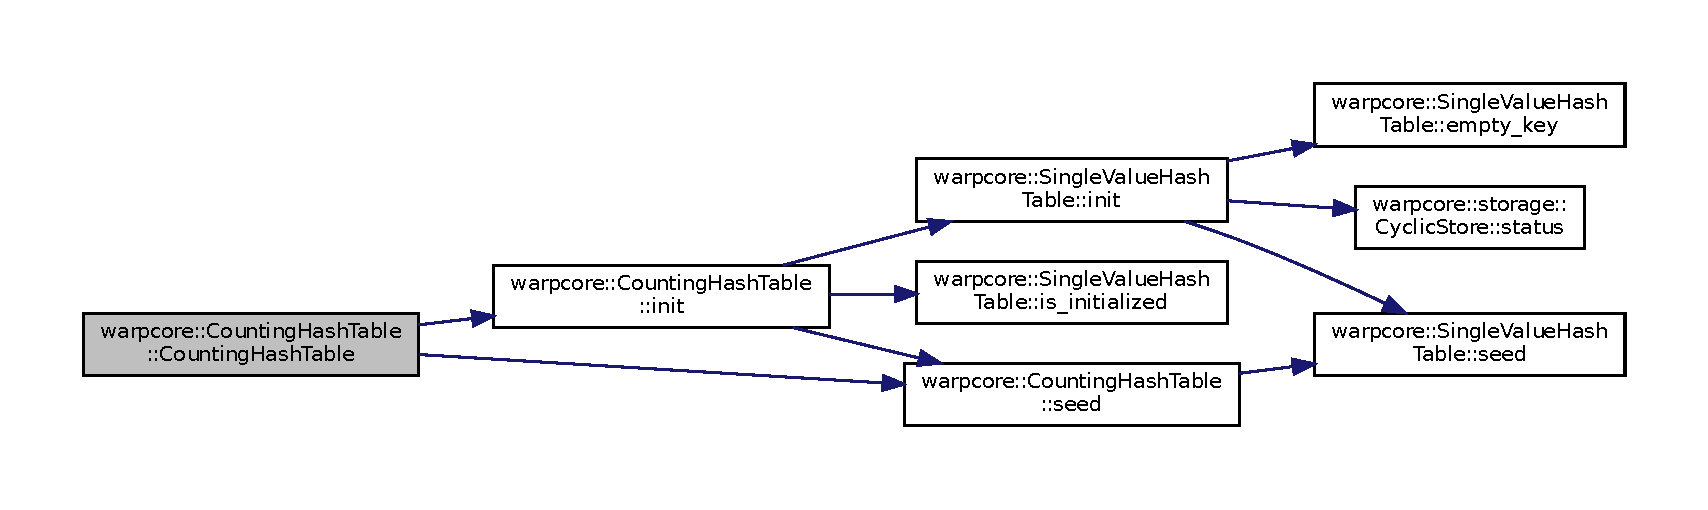
\includegraphics[width=350pt]{classwarpcore_1_1CountingHashTable_a68946e67712e7b2afb95ddb7169a26fd_cgraph}
\end{center}
\end{figure}
\mbox{\Hypertarget{classwarpcore_1_1CountingHashTable_afba99fa2513c3ca3c7708ac718d2b0fc}\label{classwarpcore_1_1CountingHashTable_afba99fa2513c3ca3c7708ac718d2b0fc}} 
\index{warpcore::CountingHashTable$<$ Key, Value, EmptyKey, TombstoneKey, ProbingScheme, TableStorage, TempMemoryBytes $>$@{warpcore::CountingHashTable$<$ Key, Value, EmptyKey, TombstoneKey, ProbingScheme, TableStorage, TempMemoryBytes $>$}!CountingHashTable@{CountingHashTable}}
\index{CountingHashTable@{CountingHashTable}!warpcore::CountingHashTable$<$ Key, Value, EmptyKey, TombstoneKey, ProbingScheme, TableStorage, TempMemoryBytes $>$@{warpcore::CountingHashTable$<$ Key, Value, EmptyKey, TombstoneKey, ProbingScheme, TableStorage, TempMemoryBytes $>$}}
\doxysubsubsection{\texorpdfstring{CountingHashTable()}{CountingHashTable()}\hspace{0.1cm}{\footnotesize\ttfamily [2/3]}}
{\footnotesize\ttfamily template$<$class Key , class Value  = index\+\_\+t, Key Empty\+Key = defaults\+::empty\+\_\+key$<$\+Key$>$(), Key Tombstone\+Key = defaults\+::tombstone\+\_\+key$<$\+Key$>$(), class Probing\+Scheme  = defaults\+::probing\+\_\+scheme\+\_\+t$<$\+Key, 4$>$, class Table\+Storage  = defaults\+::table\+\_\+storage\+\_\+t$<$\+Key, Value$>$, index\+\_\+t Temp\+Memory\+Bytes = defaults\+::temp\+\_\+memory\+\_\+bytes()$>$ \\
\+\_\+\+\_\+host\+\_\+\+\_\+\+\_\+\+\_\+device\+\_\+\+\_\+ \mbox{\hyperlink{classwarpcore_1_1CountingHashTable}{warpcore\+::\+Counting\+Hash\+Table}}$<$ Key, Value, Empty\+Key, Tombstone\+Key, Probing\+Scheme, Table\+Storage, Temp\+Memory\+Bytes $>$\+::\mbox{\hyperlink{classwarpcore_1_1CountingHashTable}{Counting\+Hash\+Table}} (\begin{DoxyParamCaption}\item[{const \mbox{\hyperlink{classwarpcore_1_1CountingHashTable}{Counting\+Hash\+Table}}$<$ Key, Value, Empty\+Key, Tombstone\+Key, Probing\+Scheme, Table\+Storage, Temp\+Memory\+Bytes $>$ \&}]{o }\end{DoxyParamCaption})\hspace{0.3cm}{\ttfamily [inline]}, {\ttfamily [noexcept]}}



copy-\/constructor (shallow) 


\begin{DoxyParams}[1]{Parameters}
\mbox{\texttt{ in}}  & {\em object} & to be copied \\
\hline
\end{DoxyParams}
\mbox{\Hypertarget{classwarpcore_1_1CountingHashTable_ab1c1ea195d10fbbdb6a70e5f3bf96623}\label{classwarpcore_1_1CountingHashTable_ab1c1ea195d10fbbdb6a70e5f3bf96623}} 
\index{warpcore::CountingHashTable$<$ Key, Value, EmptyKey, TombstoneKey, ProbingScheme, TableStorage, TempMemoryBytes $>$@{warpcore::CountingHashTable$<$ Key, Value, EmptyKey, TombstoneKey, ProbingScheme, TableStorage, TempMemoryBytes $>$}!CountingHashTable@{CountingHashTable}}
\index{CountingHashTable@{CountingHashTable}!warpcore::CountingHashTable$<$ Key, Value, EmptyKey, TombstoneKey, ProbingScheme, TableStorage, TempMemoryBytes $>$@{warpcore::CountingHashTable$<$ Key, Value, EmptyKey, TombstoneKey, ProbingScheme, TableStorage, TempMemoryBytes $>$}}
\doxysubsubsection{\texorpdfstring{CountingHashTable()}{CountingHashTable()}\hspace{0.1cm}{\footnotesize\ttfamily [3/3]}}
{\footnotesize\ttfamily template$<$class Key , class Value  = index\+\_\+t, Key Empty\+Key = defaults\+::empty\+\_\+key$<$\+Key$>$(), Key Tombstone\+Key = defaults\+::tombstone\+\_\+key$<$\+Key$>$(), class Probing\+Scheme  = defaults\+::probing\+\_\+scheme\+\_\+t$<$\+Key, 4$>$, class Table\+Storage  = defaults\+::table\+\_\+storage\+\_\+t$<$\+Key, Value$>$, index\+\_\+t Temp\+Memory\+Bytes = defaults\+::temp\+\_\+memory\+\_\+bytes()$>$ \\
\+\_\+\+\_\+host\+\_\+\+\_\+ \mbox{\hyperlink{classwarpcore_1_1CountingHashTable}{warpcore\+::\+Counting\+Hash\+Table}}$<$ Key, Value, Empty\+Key, Tombstone\+Key, Probing\+Scheme, Table\+Storage, Temp\+Memory\+Bytes $>$\+::\mbox{\hyperlink{classwarpcore_1_1CountingHashTable}{Counting\+Hash\+Table}} (\begin{DoxyParamCaption}\item[{\mbox{\hyperlink{classwarpcore_1_1CountingHashTable}{Counting\+Hash\+Table}}$<$ Key, Value, Empty\+Key, Tombstone\+Key, Probing\+Scheme, Table\+Storage, Temp\+Memory\+Bytes $>$ \&\&}]{o }\end{DoxyParamCaption})\hspace{0.3cm}{\ttfamily [inline]}, {\ttfamily [noexcept]}}



move-\/constructor 


\begin{DoxyParams}[1]{Parameters}
\mbox{\texttt{ in}}  & {\em object} & to be moved \\
\hline
\end{DoxyParams}


\doxysubsection{Member Function Documentation}
\mbox{\Hypertarget{classwarpcore_1_1CountingHashTable_a05cdc2ffc3c11c2b10d90b3d8812e96d}\label{classwarpcore_1_1CountingHashTable_a05cdc2ffc3c11c2b10d90b3d8812e96d}} 
\index{warpcore::CountingHashTable$<$ Key, Value, EmptyKey, TombstoneKey, ProbingScheme, TableStorage, TempMemoryBytes $>$@{warpcore::CountingHashTable$<$ Key, Value, EmptyKey, TombstoneKey, ProbingScheme, TableStorage, TempMemoryBytes $>$}!capacity@{capacity}}
\index{capacity@{capacity}!warpcore::CountingHashTable$<$ Key, Value, EmptyKey, TombstoneKey, ProbingScheme, TableStorage, TempMemoryBytes $>$@{warpcore::CountingHashTable$<$ Key, Value, EmptyKey, TombstoneKey, ProbingScheme, TableStorage, TempMemoryBytes $>$}}
\doxysubsubsection{\texorpdfstring{capacity()}{capacity()}}
{\footnotesize\ttfamily template$<$class Key , class Value  = index\+\_\+t, Key Empty\+Key = defaults\+::empty\+\_\+key$<$\+Key$>$(), Key Tombstone\+Key = defaults\+::tombstone\+\_\+key$<$\+Key$>$(), class Probing\+Scheme  = defaults\+::probing\+\_\+scheme\+\_\+t$<$\+Key, 4$>$, class Table\+Storage  = defaults\+::table\+\_\+storage\+\_\+t$<$\+Key, Value$>$, index\+\_\+t Temp\+Memory\+Bytes = defaults\+::temp\+\_\+memory\+\_\+bytes()$>$ \\
\+\_\+\+\_\+host\+\_\+\+\_\+\+\_\+\+\_\+device\+\_\+\+\_\+ index\+\_\+type \mbox{\hyperlink{classwarpcore_1_1CountingHashTable}{warpcore\+::\+Counting\+Hash\+Table}}$<$ Key, Value, Empty\+Key, Tombstone\+Key, Probing\+Scheme, Table\+Storage, Temp\+Memory\+Bytes $>$\+::capacity (\begin{DoxyParamCaption}{ }\end{DoxyParamCaption}) const\hspace{0.3cm}{\ttfamily [inline]}, {\ttfamily [noexcept]}}



get the capacity of the hash table 

\begin{DoxyReturn}{Returns}
number of slots in the hash table 
\end{DoxyReturn}
Here is the call graph for this function\+:
\nopagebreak
\begin{figure}[H]
\begin{center}
\leavevmode
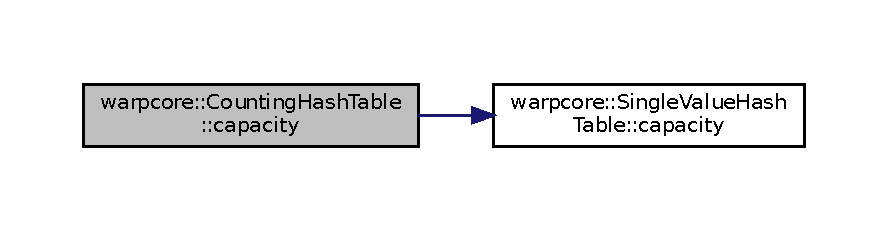
\includegraphics[width=350pt]{classwarpcore_1_1CountingHashTable_a05cdc2ffc3c11c2b10d90b3d8812e96d_cgraph}
\end{center}
\end{figure}
\mbox{\Hypertarget{classwarpcore_1_1CountingHashTable_a5efe6f4060321596322a99a28fcaef93}\label{classwarpcore_1_1CountingHashTable_a5efe6f4060321596322a99a28fcaef93}} 
\index{warpcore::CountingHashTable$<$ Key, Value, EmptyKey, TombstoneKey, ProbingScheme, TableStorage, TempMemoryBytes $>$@{warpcore::CountingHashTable$<$ Key, Value, EmptyKey, TombstoneKey, ProbingScheme, TableStorage, TempMemoryBytes $>$}!cg\_size@{cg\_size}}
\index{cg\_size@{cg\_size}!warpcore::CountingHashTable$<$ Key, Value, EmptyKey, TombstoneKey, ProbingScheme, TableStorage, TempMemoryBytes $>$@{warpcore::CountingHashTable$<$ Key, Value, EmptyKey, TombstoneKey, ProbingScheme, TableStorage, TempMemoryBytes $>$}}
\doxysubsubsection{\texorpdfstring{cg\_size()}{cg\_size()}}
{\footnotesize\ttfamily template$<$class Key , class Value  = index\+\_\+t, Key Empty\+Key = defaults\+::empty\+\_\+key$<$\+Key$>$(), Key Tombstone\+Key = defaults\+::tombstone\+\_\+key$<$\+Key$>$(), class Probing\+Scheme  = defaults\+::probing\+\_\+scheme\+\_\+t$<$\+Key, 4$>$, class Table\+Storage  = defaults\+::table\+\_\+storage\+\_\+t$<$\+Key, Value$>$, index\+\_\+t Temp\+Memory\+Bytes = defaults\+::temp\+\_\+memory\+\_\+bytes()$>$ \\
static constexpr \+\_\+\+\_\+host\+\_\+\+\_\+\+\_\+\+\_\+device\+\_\+\+\_\+ index\+\_\+type \mbox{\hyperlink{classwarpcore_1_1CountingHashTable}{warpcore\+::\+Counting\+Hash\+Table}}$<$ Key, Value, Empty\+Key, Tombstone\+Key, Probing\+Scheme, Table\+Storage, Temp\+Memory\+Bytes $>$\+::cg\+\_\+size (\begin{DoxyParamCaption}{ }\end{DoxyParamCaption})\hspace{0.3cm}{\ttfamily [inline]}, {\ttfamily [static]}, {\ttfamily [constexpr]}, {\ttfamily [noexcept]}}



get cooperative group size 

\begin{DoxyReturn}{Returns}
cooperative group size 
\end{DoxyReturn}
Here is the call graph for this function\+:
\nopagebreak
\begin{figure}[H]
\begin{center}
\leavevmode
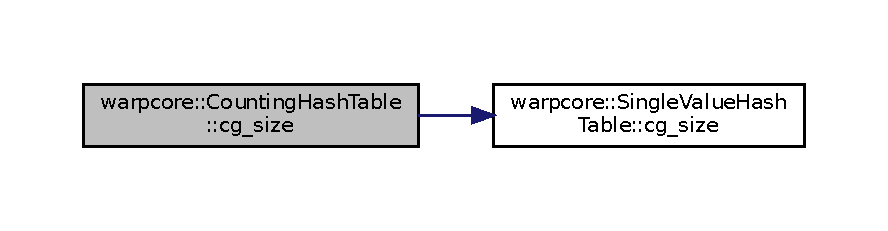
\includegraphics[width=350pt]{classwarpcore_1_1CountingHashTable_a5efe6f4060321596322a99a28fcaef93_cgraph}
\end{center}
\end{figure}
Here is the caller graph for this function\+:
\nopagebreak
\begin{figure}[H]
\begin{center}
\leavevmode
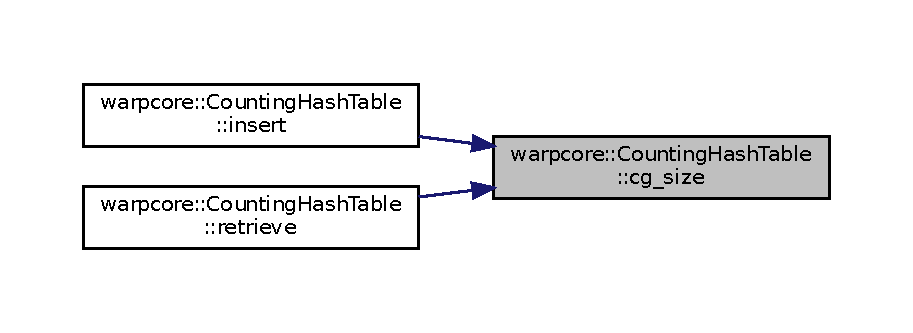
\includegraphics[width=350pt]{classwarpcore_1_1CountingHashTable_a5efe6f4060321596322a99a28fcaef93_icgraph}
\end{center}
\end{figure}
\mbox{\Hypertarget{classwarpcore_1_1CountingHashTable_a09c6eebe2c230885b14a6c7b97b30f65}\label{classwarpcore_1_1CountingHashTable_a09c6eebe2c230885b14a6c7b97b30f65}} 
\index{warpcore::CountingHashTable$<$ Key, Value, EmptyKey, TombstoneKey, ProbingScheme, TableStorage, TempMemoryBytes $>$@{warpcore::CountingHashTable$<$ Key, Value, EmptyKey, TombstoneKey, ProbingScheme, TableStorage, TempMemoryBytes $>$}!empty\_key@{empty\_key}}
\index{empty\_key@{empty\_key}!warpcore::CountingHashTable$<$ Key, Value, EmptyKey, TombstoneKey, ProbingScheme, TableStorage, TempMemoryBytes $>$@{warpcore::CountingHashTable$<$ Key, Value, EmptyKey, TombstoneKey, ProbingScheme, TableStorage, TempMemoryBytes $>$}}
\doxysubsubsection{\texorpdfstring{empty\_key()}{empty\_key()}}
{\footnotesize\ttfamily template$<$class Key , class Value  = index\+\_\+t, Key Empty\+Key = defaults\+::empty\+\_\+key$<$\+Key$>$(), Key Tombstone\+Key = defaults\+::tombstone\+\_\+key$<$\+Key$>$(), class Probing\+Scheme  = defaults\+::probing\+\_\+scheme\+\_\+t$<$\+Key, 4$>$, class Table\+Storage  = defaults\+::table\+\_\+storage\+\_\+t$<$\+Key, Value$>$, index\+\_\+t Temp\+Memory\+Bytes = defaults\+::temp\+\_\+memory\+\_\+bytes()$>$ \\
static constexpr \+\_\+\+\_\+host\+\_\+\+\_\+\+\_\+\+\_\+device\+\_\+\+\_\+ key\+\_\+type \mbox{\hyperlink{classwarpcore_1_1CountingHashTable}{warpcore\+::\+Counting\+Hash\+Table}}$<$ Key, Value, Empty\+Key, Tombstone\+Key, Probing\+Scheme, Table\+Storage, Temp\+Memory\+Bytes $>$\+::empty\+\_\+key (\begin{DoxyParamCaption}{ }\end{DoxyParamCaption})\hspace{0.3cm}{\ttfamily [inline]}, {\ttfamily [static]}, {\ttfamily [constexpr]}, {\ttfamily [noexcept]}}



get empty key 

\begin{DoxyReturn}{Returns}
empty key 
\end{DoxyReturn}
Here is the call graph for this function\+:
\nopagebreak
\begin{figure}[H]
\begin{center}
\leavevmode
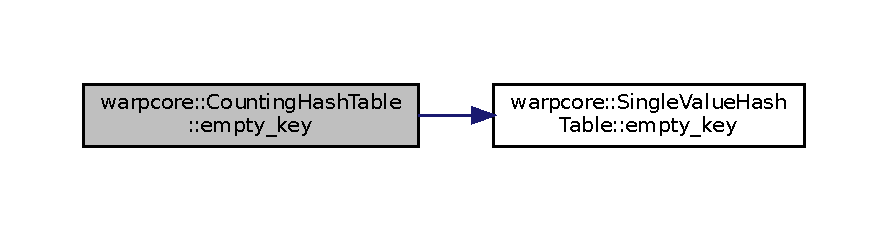
\includegraphics[width=350pt]{classwarpcore_1_1CountingHashTable_a09c6eebe2c230885b14a6c7b97b30f65_cgraph}
\end{center}
\end{figure}
\mbox{\Hypertarget{classwarpcore_1_1CountingHashTable_ac43612ae6bae1c2b01c3b2af63d7a652}\label{classwarpcore_1_1CountingHashTable_ac43612ae6bae1c2b01c3b2af63d7a652}} 
\index{warpcore::CountingHashTable$<$ Key, Value, EmptyKey, TombstoneKey, ProbingScheme, TableStorage, TempMemoryBytes $>$@{warpcore::CountingHashTable$<$ Key, Value, EmptyKey, TombstoneKey, ProbingScheme, TableStorage, TempMemoryBytes $>$}!erase@{erase}}
\index{erase@{erase}!warpcore::CountingHashTable$<$ Key, Value, EmptyKey, TombstoneKey, ProbingScheme, TableStorage, TempMemoryBytes $>$@{warpcore::CountingHashTable$<$ Key, Value, EmptyKey, TombstoneKey, ProbingScheme, TableStorage, TempMemoryBytes $>$}}
\doxysubsubsection{\texorpdfstring{erase()}{erase()}\hspace{0.1cm}{\footnotesize\ttfamily [1/2]}}
{\footnotesize\ttfamily template$<$class Key , class Value  = index\+\_\+t, Key Empty\+Key = defaults\+::empty\+\_\+key$<$\+Key$>$(), Key Tombstone\+Key = defaults\+::tombstone\+\_\+key$<$\+Key$>$(), class Probing\+Scheme  = defaults\+::probing\+\_\+scheme\+\_\+t$<$\+Key, 4$>$, class Table\+Storage  = defaults\+::table\+\_\+storage\+\_\+t$<$\+Key, Value$>$, index\+\_\+t Temp\+Memory\+Bytes = defaults\+::temp\+\_\+memory\+\_\+bytes()$>$ \\
template$<$class Status\+Handler  = defaults\+::status\+\_\+handler\+\_\+t$>$ \\
\+\_\+\+\_\+host\+\_\+\+\_\+ void \mbox{\hyperlink{classwarpcore_1_1CountingHashTable}{warpcore\+::\+Counting\+Hash\+Table}}$<$ Key, Value, Empty\+Key, Tombstone\+Key, Probing\+Scheme, Table\+Storage, Temp\+Memory\+Bytes $>$\+::erase (\begin{DoxyParamCaption}\item[{key\+\_\+type $\ast$}]{keys\+\_\+in,  }\item[{index\+\_\+type}]{num\+\_\+in,  }\item[{cuda\+Stream\+\_\+t}]{stream = {\ttfamily 0},  }\item[{index\+\_\+type}]{probing\+\_\+length = {\ttfamily defaults\+:\+:probing\+\_\+length()},  }\item[{typename Status\+Handler\+::base\+\_\+type $\ast$}]{status\+\_\+out = {\ttfamily nullptr} }\end{DoxyParamCaption})\hspace{0.3cm}{\ttfamily [inline]}, {\ttfamily [noexcept]}}



erases a set of keys from the hash table 


\begin{DoxyTemplParams}{Template Parameters}
{\em Status\+Handler} & handles status per key (see {\ttfamily \mbox{\hyperlink{namespacewarpcore_1_1status__handlers}{status\+\_\+handlers}}}) \\
\hline
\end{DoxyTemplParams}

\begin{DoxyParams}[1]{Parameters}
\mbox{\texttt{ in}}  & {\em keys\+\_\+in} & pointer to keys to erase from the hash table \\
\hline
\mbox{\texttt{ in}}  & {\em num\+\_\+in} & number of keys to erase \\
\hline
\mbox{\texttt{ in}}  & {\em stream} & C\+U\+DA stream in which this operation is executed in \\
\hline
\mbox{\texttt{ in}}  & {\em probing\+\_\+length} & maximum number of probing attempts \\
\hline
\mbox{\texttt{ out}}  & {\em status\+\_\+out} & status information (per key) \\
\hline
\end{DoxyParams}
\mbox{\Hypertarget{classwarpcore_1_1CountingHashTable_aee43cc21c75f1ad37e79604afa034363}\label{classwarpcore_1_1CountingHashTable_aee43cc21c75f1ad37e79604afa034363}} 
\index{warpcore::CountingHashTable$<$ Key, Value, EmptyKey, TombstoneKey, ProbingScheme, TableStorage, TempMemoryBytes $>$@{warpcore::CountingHashTable$<$ Key, Value, EmptyKey, TombstoneKey, ProbingScheme, TableStorage, TempMemoryBytes $>$}!erase@{erase}}
\index{erase@{erase}!warpcore::CountingHashTable$<$ Key, Value, EmptyKey, TombstoneKey, ProbingScheme, TableStorage, TempMemoryBytes $>$@{warpcore::CountingHashTable$<$ Key, Value, EmptyKey, TombstoneKey, ProbingScheme, TableStorage, TempMemoryBytes $>$}}
\doxysubsubsection{\texorpdfstring{erase()}{erase()}\hspace{0.1cm}{\footnotesize\ttfamily [2/2]}}
{\footnotesize\ttfamily template$<$class Key , class Value  = index\+\_\+t, Key Empty\+Key = defaults\+::empty\+\_\+key$<$\+Key$>$(), Key Tombstone\+Key = defaults\+::tombstone\+\_\+key$<$\+Key$>$(), class Probing\+Scheme  = defaults\+::probing\+\_\+scheme\+\_\+t$<$\+Key, 4$>$, class Table\+Storage  = defaults\+::table\+\_\+storage\+\_\+t$<$\+Key, Value$>$, index\+\_\+t Temp\+Memory\+Bytes = defaults\+::temp\+\_\+memory\+\_\+bytes()$>$ \\
\+\_\+\+\_\+device\+\_\+\+\_\+ status\+\_\+type \mbox{\hyperlink{classwarpcore_1_1CountingHashTable}{warpcore\+::\+Counting\+Hash\+Table}}$<$ Key, Value, Empty\+Key, Tombstone\+Key, Probing\+Scheme, Table\+Storage, Temp\+Memory\+Bytes $>$\+::erase (\begin{DoxyParamCaption}\item[{key\+\_\+type}]{key\+\_\+in,  }\item[{const cg\+::thread\+\_\+block\+\_\+tile$<$ \mbox{\hyperlink{classwarpcore_1_1CountingHashTable_a5efe6f4060321596322a99a28fcaef93}{cg\+\_\+size}}()$>$ \&}]{group,  }\item[{index\+\_\+type}]{probing\+\_\+length = {\ttfamily defaults\+:\+:probing\+\_\+length()} }\end{DoxyParamCaption})\hspace{0.3cm}{\ttfamily [inline]}, {\ttfamily [noexcept]}}



erases a key from the hash table 


\begin{DoxyParams}[1]{Parameters}
\mbox{\texttt{ in}}  & {\em key\+\_\+in} & key to erase from the hash table \\
\hline
\mbox{\texttt{ in}}  & {\em group} & cooperative group \\
\hline
\mbox{\texttt{ in}}  & {\em probing\+\_\+length} & maximum number of probing attempts \\
\hline
\end{DoxyParams}
\begin{DoxyReturn}{Returns}
status (per thread) 
\end{DoxyReturn}
Here is the call graph for this function\+:
\nopagebreak
\begin{figure}[H]
\begin{center}
\leavevmode
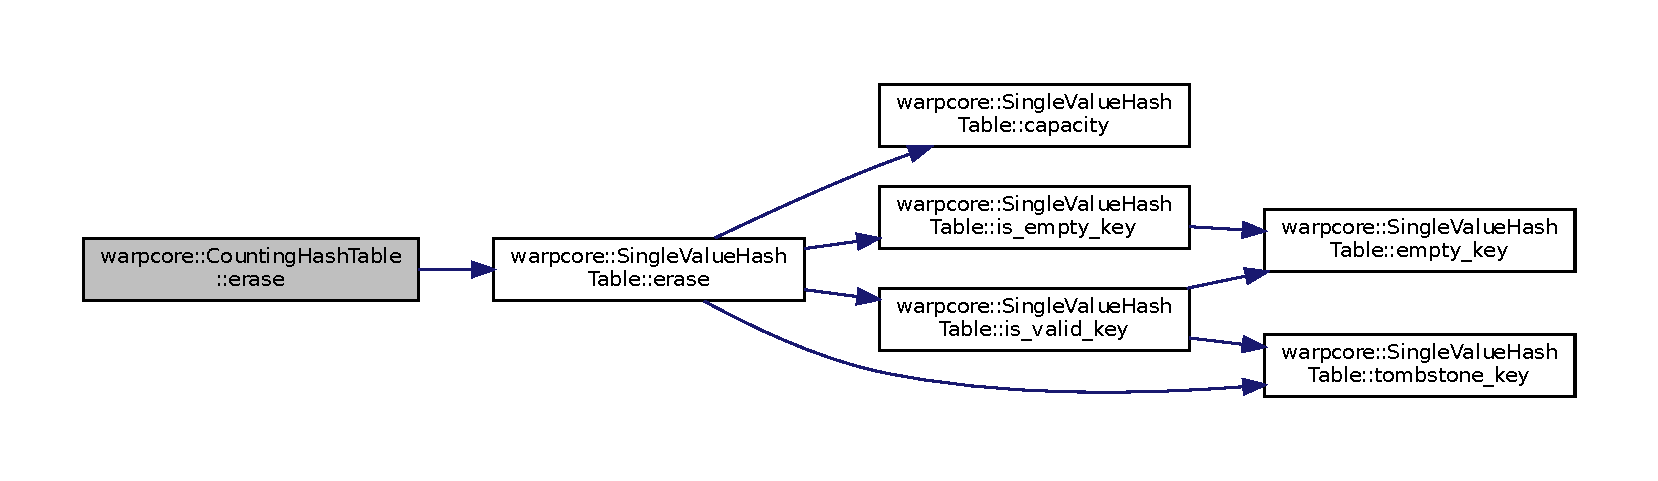
\includegraphics[width=350pt]{classwarpcore_1_1CountingHashTable_aee43cc21c75f1ad37e79604afa034363_cgraph}
\end{center}
\end{figure}
\mbox{\Hypertarget{classwarpcore_1_1CountingHashTable_aea11af31c41fe5d7369b42f2b74d276a}\label{classwarpcore_1_1CountingHashTable_aea11af31c41fe5d7369b42f2b74d276a}} 
\index{warpcore::CountingHashTable$<$ Key, Value, EmptyKey, TombstoneKey, ProbingScheme, TableStorage, TempMemoryBytes $>$@{warpcore::CountingHashTable$<$ Key, Value, EmptyKey, TombstoneKey, ProbingScheme, TableStorage, TempMemoryBytes $>$}!for\_each@{for\_each}}
\index{for\_each@{for\_each}!warpcore::CountingHashTable$<$ Key, Value, EmptyKey, TombstoneKey, ProbingScheme, TableStorage, TempMemoryBytes $>$@{warpcore::CountingHashTable$<$ Key, Value, EmptyKey, TombstoneKey, ProbingScheme, TableStorage, TempMemoryBytes $>$}}
\doxysubsubsection{\texorpdfstring{for\_each()}{for\_each()}}
{\footnotesize\ttfamily template$<$class Key , class Value  = index\+\_\+t, Key Empty\+Key = defaults\+::empty\+\_\+key$<$\+Key$>$(), Key Tombstone\+Key = defaults\+::tombstone\+\_\+key$<$\+Key$>$(), class Probing\+Scheme  = defaults\+::probing\+\_\+scheme\+\_\+t$<$\+Key, 4$>$, class Table\+Storage  = defaults\+::table\+\_\+storage\+\_\+t$<$\+Key, Value$>$, index\+\_\+t Temp\+Memory\+Bytes = defaults\+::temp\+\_\+memory\+\_\+bytes()$>$ \\
template$<$class Func $>$ \\
\+\_\+\+\_\+host\+\_\+\+\_\+ void \mbox{\hyperlink{classwarpcore_1_1CountingHashTable}{warpcore\+::\+Counting\+Hash\+Table}}$<$ Key, Value, Empty\+Key, Tombstone\+Key, Probing\+Scheme, Table\+Storage, Temp\+Memory\+Bytes $>$\+::for\+\_\+each (\begin{DoxyParamCaption}\item[{Func}]{f,  }\item[{cuda\+Stream\+\_\+t}]{stream = {\ttfamily 0},  }\item[{index\+\_\+type}]{smem\+\_\+bytes = {\ttfamily 0} }\end{DoxyParamCaption}) const\hspace{0.3cm}{\ttfamily [inline]}, {\ttfamily [noexcept]}}



applies a funtion on all key value pairs inside the table 


\begin{DoxyTemplParams}{Template Parameters}
{\em Func} & type of map i.\+e. C\+U\+DA device lambda \\
\hline
\end{DoxyTemplParams}

\begin{DoxyParams}[1]{Parameters}
\mbox{\texttt{ in}}  & {\em f} & map to apply \\
\hline
\mbox{\texttt{ in}}  & {\em stream} & C\+U\+DA stream in which this operation is executed in \\
\hline
\mbox{\texttt{ in}}  & {\em size} & of shared memory to reserve for this execution \\
\hline
\end{DoxyParams}
\mbox{\Hypertarget{classwarpcore_1_1CountingHashTable_a8b7a93faf9c5746c2665b4b775f9de88}\label{classwarpcore_1_1CountingHashTable_a8b7a93faf9c5746c2665b4b775f9de88}} 
\index{warpcore::CountingHashTable$<$ Key, Value, EmptyKey, TombstoneKey, ProbingScheme, TableStorage, TempMemoryBytes $>$@{warpcore::CountingHashTable$<$ Key, Value, EmptyKey, TombstoneKey, ProbingScheme, TableStorage, TempMemoryBytes $>$}!init@{init}}
\index{init@{init}!warpcore::CountingHashTable$<$ Key, Value, EmptyKey, TombstoneKey, ProbingScheme, TableStorage, TempMemoryBytes $>$@{warpcore::CountingHashTable$<$ Key, Value, EmptyKey, TombstoneKey, ProbingScheme, TableStorage, TempMemoryBytes $>$}}
\doxysubsubsection{\texorpdfstring{init()}{init()}\hspace{0.1cm}{\footnotesize\ttfamily [1/2]}}
{\footnotesize\ttfamily template$<$class Key , class Value  = index\+\_\+t, Key Empty\+Key = defaults\+::empty\+\_\+key$<$\+Key$>$(), Key Tombstone\+Key = defaults\+::tombstone\+\_\+key$<$\+Key$>$(), class Probing\+Scheme  = defaults\+::probing\+\_\+scheme\+\_\+t$<$\+Key, 4$>$, class Table\+Storage  = defaults\+::table\+\_\+storage\+\_\+t$<$\+Key, Value$>$, index\+\_\+t Temp\+Memory\+Bytes = defaults\+::temp\+\_\+memory\+\_\+bytes()$>$ \\
\+\_\+\+\_\+host\+\_\+\+\_\+ void \mbox{\hyperlink{classwarpcore_1_1CountingHashTable}{warpcore\+::\+Counting\+Hash\+Table}}$<$ Key, Value, Empty\+Key, Tombstone\+Key, Probing\+Scheme, Table\+Storage, Temp\+Memory\+Bytes $>$\+::init (\begin{DoxyParamCaption}\item[{const cuda\+Stream\+\_\+t}]{stream = {\ttfamily 0} }\end{DoxyParamCaption})\hspace{0.3cm}{\ttfamily [inline]}, {\ttfamily [noexcept]}}



(re)initialize the hash table 


\begin{DoxyParams}[1]{Parameters}
\mbox{\texttt{ in}}  & {\em stream} & C\+U\+DA stream in which this operation is executed in \\
\hline
\end{DoxyParams}
Here is the call graph for this function\+:
\nopagebreak
\begin{figure}[H]
\begin{center}
\leavevmode
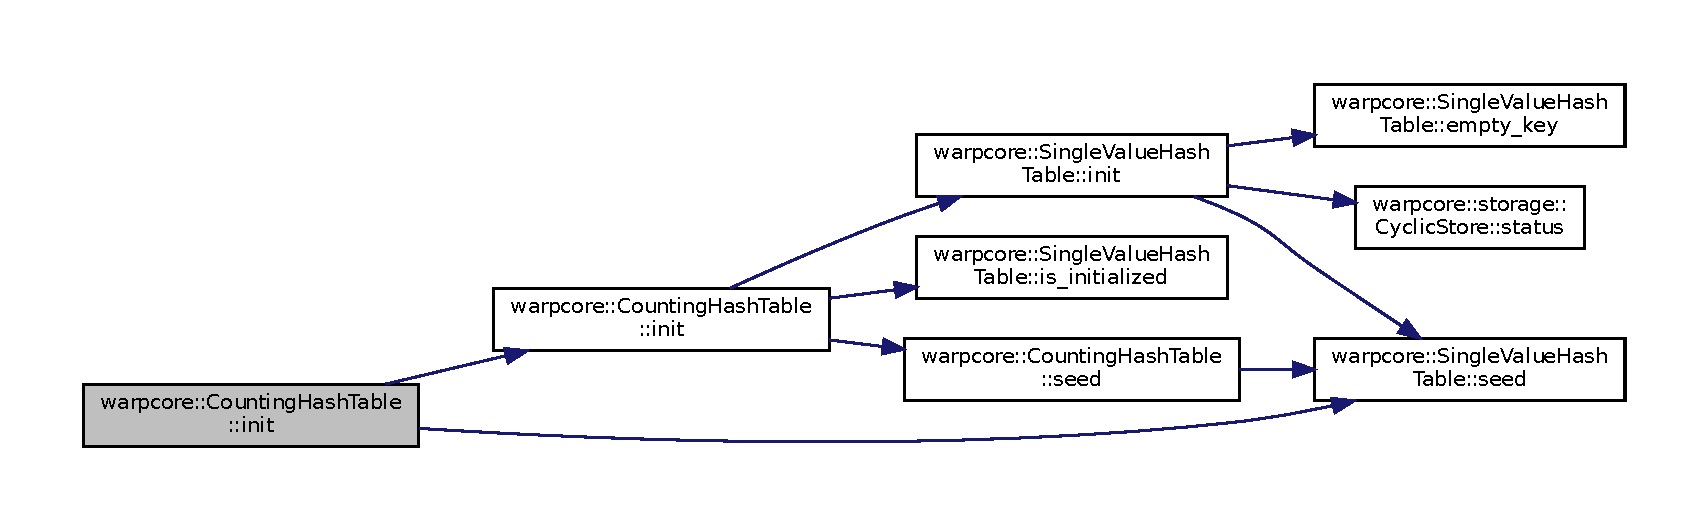
\includegraphics[width=350pt]{classwarpcore_1_1CountingHashTable_a8b7a93faf9c5746c2665b4b775f9de88_cgraph}
\end{center}
\end{figure}
\mbox{\Hypertarget{classwarpcore_1_1CountingHashTable_acb401fb2d38c59e086a1bedf68d4815f}\label{classwarpcore_1_1CountingHashTable_acb401fb2d38c59e086a1bedf68d4815f}} 
\index{warpcore::CountingHashTable$<$ Key, Value, EmptyKey, TombstoneKey, ProbingScheme, TableStorage, TempMemoryBytes $>$@{warpcore::CountingHashTable$<$ Key, Value, EmptyKey, TombstoneKey, ProbingScheme, TableStorage, TempMemoryBytes $>$}!init@{init}}
\index{init@{init}!warpcore::CountingHashTable$<$ Key, Value, EmptyKey, TombstoneKey, ProbingScheme, TableStorage, TempMemoryBytes $>$@{warpcore::CountingHashTable$<$ Key, Value, EmptyKey, TombstoneKey, ProbingScheme, TableStorage, TempMemoryBytes $>$}}
\doxysubsubsection{\texorpdfstring{init()}{init()}\hspace{0.1cm}{\footnotesize\ttfamily [2/2]}}
{\footnotesize\ttfamily template$<$class Key , class Value  = index\+\_\+t, Key Empty\+Key = defaults\+::empty\+\_\+key$<$\+Key$>$(), Key Tombstone\+Key = defaults\+::tombstone\+\_\+key$<$\+Key$>$(), class Probing\+Scheme  = defaults\+::probing\+\_\+scheme\+\_\+t$<$\+Key, 4$>$, class Table\+Storage  = defaults\+::table\+\_\+storage\+\_\+t$<$\+Key, Value$>$, index\+\_\+t Temp\+Memory\+Bytes = defaults\+::temp\+\_\+memory\+\_\+bytes()$>$ \\
\+\_\+\+\_\+host\+\_\+\+\_\+ void \mbox{\hyperlink{classwarpcore_1_1CountingHashTable}{warpcore\+::\+Counting\+Hash\+Table}}$<$ Key, Value, Empty\+Key, Tombstone\+Key, Probing\+Scheme, Table\+Storage, Temp\+Memory\+Bytes $>$\+::init (\begin{DoxyParamCaption}\item[{const key\+\_\+type}]{seed,  }\item[{const cuda\+Stream\+\_\+t}]{stream = {\ttfamily 0} }\end{DoxyParamCaption})\hspace{0.3cm}{\ttfamily [inline]}, {\ttfamily [noexcept]}}



(re)initialize the hash table 


\begin{DoxyParams}[1]{Parameters}
\mbox{\texttt{ in}}  & {\em seed} & random seed \\
\hline
\mbox{\texttt{ in}}  & {\em stream} & C\+U\+DA stream in which this operation is executed in \\
\hline
\end{DoxyParams}
Here is the call graph for this function\+:
\nopagebreak
\begin{figure}[H]
\begin{center}
\leavevmode
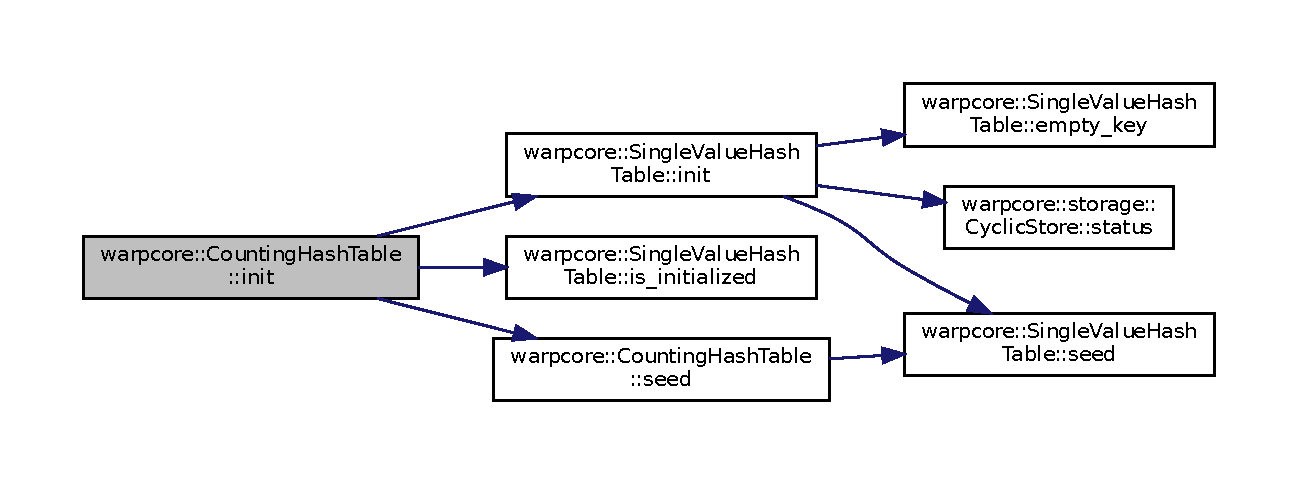
\includegraphics[width=350pt]{classwarpcore_1_1CountingHashTable_acb401fb2d38c59e086a1bedf68d4815f_cgraph}
\end{center}
\end{figure}
Here is the caller graph for this function\+:
\nopagebreak
\begin{figure}[H]
\begin{center}
\leavevmode
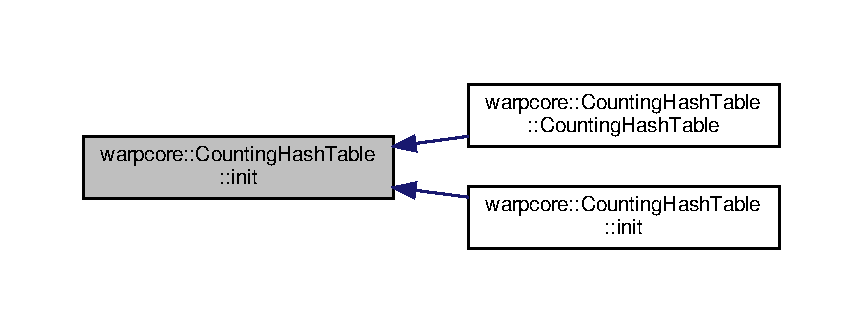
\includegraphics[width=350pt]{classwarpcore_1_1CountingHashTable_acb401fb2d38c59e086a1bedf68d4815f_icgraph}
\end{center}
\end{figure}
\mbox{\Hypertarget{classwarpcore_1_1CountingHashTable_a36d896f2f66465925ea21a9f01bb12f3}\label{classwarpcore_1_1CountingHashTable_a36d896f2f66465925ea21a9f01bb12f3}} 
\index{warpcore::CountingHashTable$<$ Key, Value, EmptyKey, TombstoneKey, ProbingScheme, TableStorage, TempMemoryBytes $>$@{warpcore::CountingHashTable$<$ Key, Value, EmptyKey, TombstoneKey, ProbingScheme, TableStorage, TempMemoryBytes $>$}!insert@{insert}}
\index{insert@{insert}!warpcore::CountingHashTable$<$ Key, Value, EmptyKey, TombstoneKey, ProbingScheme, TableStorage, TempMemoryBytes $>$@{warpcore::CountingHashTable$<$ Key, Value, EmptyKey, TombstoneKey, ProbingScheme, TableStorage, TempMemoryBytes $>$}}
\doxysubsubsection{\texorpdfstring{insert()}{insert()}\hspace{0.1cm}{\footnotesize\ttfamily [1/2]}}
{\footnotesize\ttfamily template$<$class Key , class Value  = index\+\_\+t, Key Empty\+Key = defaults\+::empty\+\_\+key$<$\+Key$>$(), Key Tombstone\+Key = defaults\+::tombstone\+\_\+key$<$\+Key$>$(), class Probing\+Scheme  = defaults\+::probing\+\_\+scheme\+\_\+t$<$\+Key, 4$>$, class Table\+Storage  = defaults\+::table\+\_\+storage\+\_\+t$<$\+Key, Value$>$, index\+\_\+t Temp\+Memory\+Bytes = defaults\+::temp\+\_\+memory\+\_\+bytes()$>$ \\
template$<$class Status\+Handler  = defaults\+::status\+\_\+handler\+\_\+t$>$ \\
\+\_\+\+\_\+host\+\_\+\+\_\+ void \mbox{\hyperlink{classwarpcore_1_1CountingHashTable}{warpcore\+::\+Counting\+Hash\+Table}}$<$ Key, Value, Empty\+Key, Tombstone\+Key, Probing\+Scheme, Table\+Storage, Temp\+Memory\+Bytes $>$\+::insert (\begin{DoxyParamCaption}\item[{key\+\_\+type $\ast$}]{keys\+\_\+in,  }\item[{index\+\_\+type}]{num\+\_\+in,  }\item[{cuda\+Stream\+\_\+t}]{stream = {\ttfamily 0},  }\item[{index\+\_\+type}]{probing\+\_\+length = {\ttfamily defaults\+:\+:probing\+\_\+length()},  }\item[{typename Status\+Handler\+::base\+\_\+type $\ast$}]{status\+\_\+out = {\ttfamily nullptr} }\end{DoxyParamCaption})\hspace{0.3cm}{\ttfamily [inline]}, {\ttfamily [noexcept]}}



insert a set of keys into the hash table 


\begin{DoxyTemplParams}{Template Parameters}
{\em Status\+Handler} & handles status per key (see {\ttfamily \mbox{\hyperlink{namespacewarpcore_1_1status__handlers}{status\+\_\+handlers}}}) \\
\hline
\end{DoxyTemplParams}

\begin{DoxyParams}[1]{Parameters}
\mbox{\texttt{ in}}  & {\em keys\+\_\+in} & pointer to keys to insert into the hash table \\
\hline
\mbox{\texttt{ in}}  & {\em num\+\_\+in} & number of keys to insert \\
\hline
\mbox{\texttt{ in}}  & {\em stream} & C\+U\+DA stream in which this operation is executed in \\
\hline
\mbox{\texttt{ in}}  & {\em probing\+\_\+length} & maximum number of probing attempts \\
\hline
\mbox{\texttt{ out}}  & {\em status\+\_\+out} & status information per key \\
\hline
\end{DoxyParams}
Here is the call graph for this function\+:
\nopagebreak
\begin{figure}[H]
\begin{center}
\leavevmode
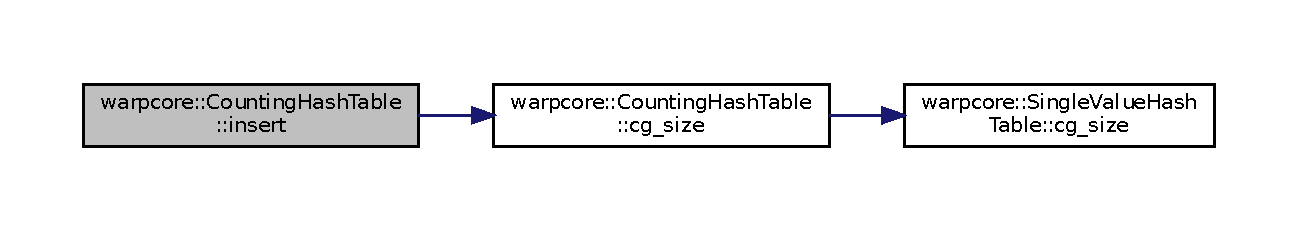
\includegraphics[width=350pt]{classwarpcore_1_1CountingHashTable_a36d896f2f66465925ea21a9f01bb12f3_cgraph}
\end{center}
\end{figure}
\mbox{\Hypertarget{classwarpcore_1_1CountingHashTable_a2cad25fea134d836cf1b75f67d6b38ac}\label{classwarpcore_1_1CountingHashTable_a2cad25fea134d836cf1b75f67d6b38ac}} 
\index{warpcore::CountingHashTable$<$ Key, Value, EmptyKey, TombstoneKey, ProbingScheme, TableStorage, TempMemoryBytes $>$@{warpcore::CountingHashTable$<$ Key, Value, EmptyKey, TombstoneKey, ProbingScheme, TableStorage, TempMemoryBytes $>$}!insert@{insert}}
\index{insert@{insert}!warpcore::CountingHashTable$<$ Key, Value, EmptyKey, TombstoneKey, ProbingScheme, TableStorage, TempMemoryBytes $>$@{warpcore::CountingHashTable$<$ Key, Value, EmptyKey, TombstoneKey, ProbingScheme, TableStorage, TempMemoryBytes $>$}}
\doxysubsubsection{\texorpdfstring{insert()}{insert()}\hspace{0.1cm}{\footnotesize\ttfamily [2/2]}}
{\footnotesize\ttfamily template$<$class Key , class Value  = index\+\_\+t, Key Empty\+Key = defaults\+::empty\+\_\+key$<$\+Key$>$(), Key Tombstone\+Key = defaults\+::tombstone\+\_\+key$<$\+Key$>$(), class Probing\+Scheme  = defaults\+::probing\+\_\+scheme\+\_\+t$<$\+Key, 4$>$, class Table\+Storage  = defaults\+::table\+\_\+storage\+\_\+t$<$\+Key, Value$>$, index\+\_\+t Temp\+Memory\+Bytes = defaults\+::temp\+\_\+memory\+\_\+bytes()$>$ \\
\+\_\+\+\_\+device\+\_\+\+\_\+ status\+\_\+type \mbox{\hyperlink{classwarpcore_1_1CountingHashTable}{warpcore\+::\+Counting\+Hash\+Table}}$<$ Key, Value, Empty\+Key, Tombstone\+Key, Probing\+Scheme, Table\+Storage, Temp\+Memory\+Bytes $>$\+::insert (\begin{DoxyParamCaption}\item[{key\+\_\+type}]{key\+\_\+in,  }\item[{const cg\+::thread\+\_\+block\+\_\+tile$<$ \mbox{\hyperlink{classwarpcore_1_1CountingHashTable_a5efe6f4060321596322a99a28fcaef93}{cg\+\_\+size}}()$>$ \&}]{group,  }\item[{index\+\_\+type}]{probing\+\_\+length = {\ttfamily defaults\+:\+:probing\+\_\+length()} }\end{DoxyParamCaption})\hspace{0.3cm}{\ttfamily [inline]}, {\ttfamily [noexcept]}}



inserts a key into the hash table 


\begin{DoxyParams}[1]{Parameters}
\mbox{\texttt{ in}}  & {\em key\+\_\+in} & key to insert into the hash table \\
\hline
\mbox{\texttt{ in}}  & {\em group} & cooperative group \\
\hline
\mbox{\texttt{ in}}  & {\em probing\+\_\+length} & maximum number of probing attempts \\
\hline
\end{DoxyParams}
\begin{DoxyReturn}{Returns}
status (per thread) 
\end{DoxyReturn}
\mbox{\Hypertarget{classwarpcore_1_1CountingHashTable_abd203ab693aa931917013e11c23d444c}\label{classwarpcore_1_1CountingHashTable_abd203ab693aa931917013e11c23d444c}} 
\index{warpcore::CountingHashTable$<$ Key, Value, EmptyKey, TombstoneKey, ProbingScheme, TableStorage, TempMemoryBytes $>$@{warpcore::CountingHashTable$<$ Key, Value, EmptyKey, TombstoneKey, ProbingScheme, TableStorage, TempMemoryBytes $>$}!is\_copy@{is\_copy}}
\index{is\_copy@{is\_copy}!warpcore::CountingHashTable$<$ Key, Value, EmptyKey, TombstoneKey, ProbingScheme, TableStorage, TempMemoryBytes $>$@{warpcore::CountingHashTable$<$ Key, Value, EmptyKey, TombstoneKey, ProbingScheme, TableStorage, TempMemoryBytes $>$}}
\doxysubsubsection{\texorpdfstring{is\_copy()}{is\_copy()}}
{\footnotesize\ttfamily template$<$class Key , class Value  = index\+\_\+t, Key Empty\+Key = defaults\+::empty\+\_\+key$<$\+Key$>$(), Key Tombstone\+Key = defaults\+::tombstone\+\_\+key$<$\+Key$>$(), class Probing\+Scheme  = defaults\+::probing\+\_\+scheme\+\_\+t$<$\+Key, 4$>$, class Table\+Storage  = defaults\+::table\+\_\+storage\+\_\+t$<$\+Key, Value$>$, index\+\_\+t Temp\+Memory\+Bytes = defaults\+::temp\+\_\+memory\+\_\+bytes()$>$ \\
\+\_\+\+\_\+host\+\_\+\+\_\+\+\_\+\+\_\+device\+\_\+\+\_\+ bool \mbox{\hyperlink{classwarpcore_1_1CountingHashTable}{warpcore\+::\+Counting\+Hash\+Table}}$<$ Key, Value, Empty\+Key, Tombstone\+Key, Probing\+Scheme, Table\+Storage, Temp\+Memory\+Bytes $>$\+::is\+\_\+copy (\begin{DoxyParamCaption}{ }\end{DoxyParamCaption}) const\hspace{0.3cm}{\ttfamily [inline]}, {\ttfamily [noexcept]}}



indicates if this object is a shallow copy 

\begin{DoxyReturn}{Returns}
{\ttfamily bool} 
\end{DoxyReturn}
\mbox{\Hypertarget{classwarpcore_1_1CountingHashTable_a7cf82f559b57bed446328aab53ffcdd2}\label{classwarpcore_1_1CountingHashTable_a7cf82f559b57bed446328aab53ffcdd2}} 
\index{warpcore::CountingHashTable$<$ Key, Value, EmptyKey, TombstoneKey, ProbingScheme, TableStorage, TempMemoryBytes $>$@{warpcore::CountingHashTable$<$ Key, Value, EmptyKey, TombstoneKey, ProbingScheme, TableStorage, TempMemoryBytes $>$}!is\_empty\_key@{is\_empty\_key}}
\index{is\_empty\_key@{is\_empty\_key}!warpcore::CountingHashTable$<$ Key, Value, EmptyKey, TombstoneKey, ProbingScheme, TableStorage, TempMemoryBytes $>$@{warpcore::CountingHashTable$<$ Key, Value, EmptyKey, TombstoneKey, ProbingScheme, TableStorage, TempMemoryBytes $>$}}
\doxysubsubsection{\texorpdfstring{is\_empty\_key()}{is\_empty\_key()}}
{\footnotesize\ttfamily template$<$class Key , class Value  = index\+\_\+t, Key Empty\+Key = defaults\+::empty\+\_\+key$<$\+Key$>$(), Key Tombstone\+Key = defaults\+::tombstone\+\_\+key$<$\+Key$>$(), class Probing\+Scheme  = defaults\+::probing\+\_\+scheme\+\_\+t$<$\+Key, 4$>$, class Table\+Storage  = defaults\+::table\+\_\+storage\+\_\+t$<$\+Key, Value$>$, index\+\_\+t Temp\+Memory\+Bytes = defaults\+::temp\+\_\+memory\+\_\+bytes()$>$ \\
static constexpr \+\_\+\+\_\+host\+\_\+\+\_\+\+\_\+\+\_\+device\+\_\+\+\_\+ bool \mbox{\hyperlink{classwarpcore_1_1CountingHashTable}{warpcore\+::\+Counting\+Hash\+Table}}$<$ Key, Value, Empty\+Key, Tombstone\+Key, Probing\+Scheme, Table\+Storage, Temp\+Memory\+Bytes $>$\+::is\+\_\+empty\+\_\+key (\begin{DoxyParamCaption}\item[{key\+\_\+type}]{key }\end{DoxyParamCaption})\hspace{0.3cm}{\ttfamily [inline]}, {\ttfamily [static]}, {\ttfamily [constexpr]}, {\ttfamily [noexcept]}}



checks if {\ttfamily key} is equal to {\ttfamily Empty\+Key} 

\begin{DoxyReturn}{Returns}
{\ttfamily bool} 
\end{DoxyReturn}
Here is the call graph for this function\+:
\nopagebreak
\begin{figure}[H]
\begin{center}
\leavevmode
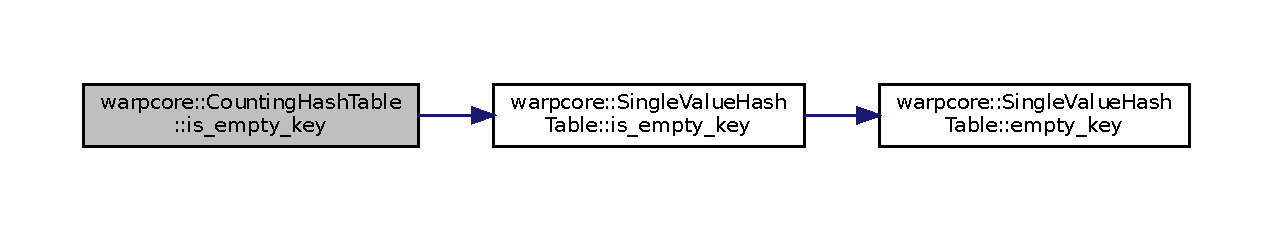
\includegraphics[width=350pt]{classwarpcore_1_1CountingHashTable_a7cf82f559b57bed446328aab53ffcdd2_cgraph}
\end{center}
\end{figure}
\mbox{\Hypertarget{classwarpcore_1_1CountingHashTable_ad4faa63cd0e6613135c12733c2d9fb6f}\label{classwarpcore_1_1CountingHashTable_ad4faa63cd0e6613135c12733c2d9fb6f}} 
\index{warpcore::CountingHashTable$<$ Key, Value, EmptyKey, TombstoneKey, ProbingScheme, TableStorage, TempMemoryBytes $>$@{warpcore::CountingHashTable$<$ Key, Value, EmptyKey, TombstoneKey, ProbingScheme, TableStorage, TempMemoryBytes $>$}!is\_tombstone\_key@{is\_tombstone\_key}}
\index{is\_tombstone\_key@{is\_tombstone\_key}!warpcore::CountingHashTable$<$ Key, Value, EmptyKey, TombstoneKey, ProbingScheme, TableStorage, TempMemoryBytes $>$@{warpcore::CountingHashTable$<$ Key, Value, EmptyKey, TombstoneKey, ProbingScheme, TableStorage, TempMemoryBytes $>$}}
\doxysubsubsection{\texorpdfstring{is\_tombstone\_key()}{is\_tombstone\_key()}}
{\footnotesize\ttfamily template$<$class Key , class Value  = index\+\_\+t, Key Empty\+Key = defaults\+::empty\+\_\+key$<$\+Key$>$(), Key Tombstone\+Key = defaults\+::tombstone\+\_\+key$<$\+Key$>$(), class Probing\+Scheme  = defaults\+::probing\+\_\+scheme\+\_\+t$<$\+Key, 4$>$, class Table\+Storage  = defaults\+::table\+\_\+storage\+\_\+t$<$\+Key, Value$>$, index\+\_\+t Temp\+Memory\+Bytes = defaults\+::temp\+\_\+memory\+\_\+bytes()$>$ \\
static constexpr \+\_\+\+\_\+host\+\_\+\+\_\+\+\_\+\+\_\+device\+\_\+\+\_\+ bool \mbox{\hyperlink{classwarpcore_1_1CountingHashTable}{warpcore\+::\+Counting\+Hash\+Table}}$<$ Key, Value, Empty\+Key, Tombstone\+Key, Probing\+Scheme, Table\+Storage, Temp\+Memory\+Bytes $>$\+::is\+\_\+tombstone\+\_\+key (\begin{DoxyParamCaption}\item[{key\+\_\+type}]{key }\end{DoxyParamCaption})\hspace{0.3cm}{\ttfamily [inline]}, {\ttfamily [static]}, {\ttfamily [constexpr]}, {\ttfamily [noexcept]}}



checks if {\ttfamily key} is equal to {\ttfamily Tombstone\+Key} 

\begin{DoxyReturn}{Returns}
{\ttfamily bool} 
\end{DoxyReturn}
Here is the call graph for this function\+:
\nopagebreak
\begin{figure}[H]
\begin{center}
\leavevmode
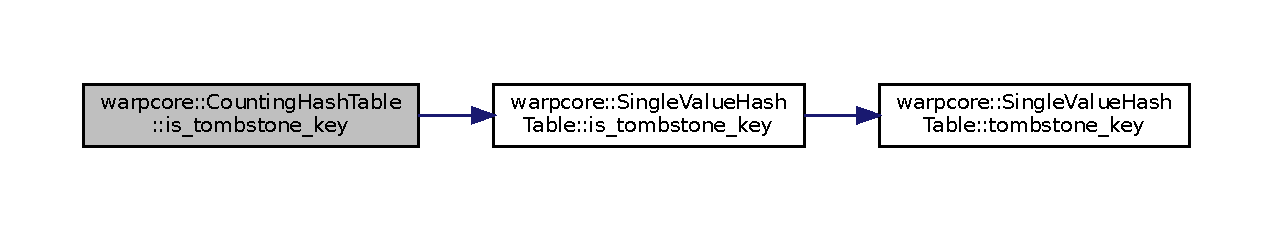
\includegraphics[width=350pt]{classwarpcore_1_1CountingHashTable_ad4faa63cd0e6613135c12733c2d9fb6f_cgraph}
\end{center}
\end{figure}
\mbox{\Hypertarget{classwarpcore_1_1CountingHashTable_a28bd96a747e0acd2f0136d74a44612d4}\label{classwarpcore_1_1CountingHashTable_a28bd96a747e0acd2f0136d74a44612d4}} 
\index{warpcore::CountingHashTable$<$ Key, Value, EmptyKey, TombstoneKey, ProbingScheme, TableStorage, TempMemoryBytes $>$@{warpcore::CountingHashTable$<$ Key, Value, EmptyKey, TombstoneKey, ProbingScheme, TableStorage, TempMemoryBytes $>$}!is\_valid\_key@{is\_valid\_key}}
\index{is\_valid\_key@{is\_valid\_key}!warpcore::CountingHashTable$<$ Key, Value, EmptyKey, TombstoneKey, ProbingScheme, TableStorage, TempMemoryBytes $>$@{warpcore::CountingHashTable$<$ Key, Value, EmptyKey, TombstoneKey, ProbingScheme, TableStorage, TempMemoryBytes $>$}}
\doxysubsubsection{\texorpdfstring{is\_valid\_key()}{is\_valid\_key()}}
{\footnotesize\ttfamily template$<$class Key , class Value  = index\+\_\+t, Key Empty\+Key = defaults\+::empty\+\_\+key$<$\+Key$>$(), Key Tombstone\+Key = defaults\+::tombstone\+\_\+key$<$\+Key$>$(), class Probing\+Scheme  = defaults\+::probing\+\_\+scheme\+\_\+t$<$\+Key, 4$>$, class Table\+Storage  = defaults\+::table\+\_\+storage\+\_\+t$<$\+Key, Value$>$, index\+\_\+t Temp\+Memory\+Bytes = defaults\+::temp\+\_\+memory\+\_\+bytes()$>$ \\
static constexpr \+\_\+\+\_\+host\+\_\+\+\_\+\+\_\+\+\_\+device\+\_\+\+\_\+ bool \mbox{\hyperlink{classwarpcore_1_1CountingHashTable}{warpcore\+::\+Counting\+Hash\+Table}}$<$ Key, Value, Empty\+Key, Tombstone\+Key, Probing\+Scheme, Table\+Storage, Temp\+Memory\+Bytes $>$\+::is\+\_\+valid\+\_\+key (\begin{DoxyParamCaption}\item[{key\+\_\+type}]{key }\end{DoxyParamCaption})\hspace{0.3cm}{\ttfamily [inline]}, {\ttfamily [static]}, {\ttfamily [constexpr]}, {\ttfamily [noexcept]}}



checks if {\ttfamily key} is equal to {\ttfamily }(Empty\+Key$\vert$$\vert$\+Tombstone\+Key) 

\begin{DoxyReturn}{Returns}
{\ttfamily bool} 
\end{DoxyReturn}
Here is the call graph for this function\+:
\nopagebreak
\begin{figure}[H]
\begin{center}
\leavevmode
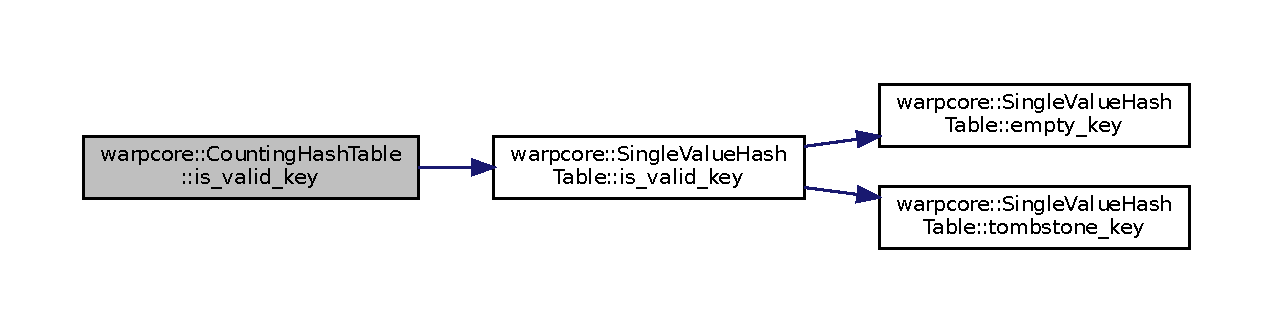
\includegraphics[width=350pt]{classwarpcore_1_1CountingHashTable_a28bd96a747e0acd2f0136d74a44612d4_cgraph}
\end{center}
\end{figure}
\mbox{\Hypertarget{classwarpcore_1_1CountingHashTable_ad4a829b15a3add41133437c17ab6bf67}\label{classwarpcore_1_1CountingHashTable_ad4a829b15a3add41133437c17ab6bf67}} 
\index{warpcore::CountingHashTable$<$ Key, Value, EmptyKey, TombstoneKey, ProbingScheme, TableStorage, TempMemoryBytes $>$@{warpcore::CountingHashTable$<$ Key, Value, EmptyKey, TombstoneKey, ProbingScheme, TableStorage, TempMemoryBytes $>$}!load\_factor@{load\_factor}}
\index{load\_factor@{load\_factor}!warpcore::CountingHashTable$<$ Key, Value, EmptyKey, TombstoneKey, ProbingScheme, TableStorage, TempMemoryBytes $>$@{warpcore::CountingHashTable$<$ Key, Value, EmptyKey, TombstoneKey, ProbingScheme, TableStorage, TempMemoryBytes $>$}}
\doxysubsubsection{\texorpdfstring{load\_factor()}{load\_factor()}}
{\footnotesize\ttfamily template$<$class Key , class Value  = index\+\_\+t, Key Empty\+Key = defaults\+::empty\+\_\+key$<$\+Key$>$(), Key Tombstone\+Key = defaults\+::tombstone\+\_\+key$<$\+Key$>$(), class Probing\+Scheme  = defaults\+::probing\+\_\+scheme\+\_\+t$<$\+Key, 4$>$, class Table\+Storage  = defaults\+::table\+\_\+storage\+\_\+t$<$\+Key, Value$>$, index\+\_\+t Temp\+Memory\+Bytes = defaults\+::temp\+\_\+memory\+\_\+bytes()$>$ \\
\+\_\+\+\_\+host\+\_\+\+\_\+ float \mbox{\hyperlink{classwarpcore_1_1CountingHashTable}{warpcore\+::\+Counting\+Hash\+Table}}$<$ Key, Value, Empty\+Key, Tombstone\+Key, Probing\+Scheme, Table\+Storage, Temp\+Memory\+Bytes $>$\+::load\+\_\+factor (\begin{DoxyParamCaption}\item[{cuda\+Stream\+\_\+t}]{stream = {\ttfamily 0} }\end{DoxyParamCaption}) const\hspace{0.3cm}{\ttfamily [inline]}, {\ttfamily [noexcept]}}



current load factor of the hash table 


\begin{DoxyParams}{Parameters}
{\em stream} & C\+U\+DA stream in which this operation is executed in \\
\hline
\end{DoxyParams}
\begin{DoxyReturn}{Returns}
load factor 
\end{DoxyReturn}
Here is the call graph for this function\+:
\nopagebreak
\begin{figure}[H]
\begin{center}
\leavevmode
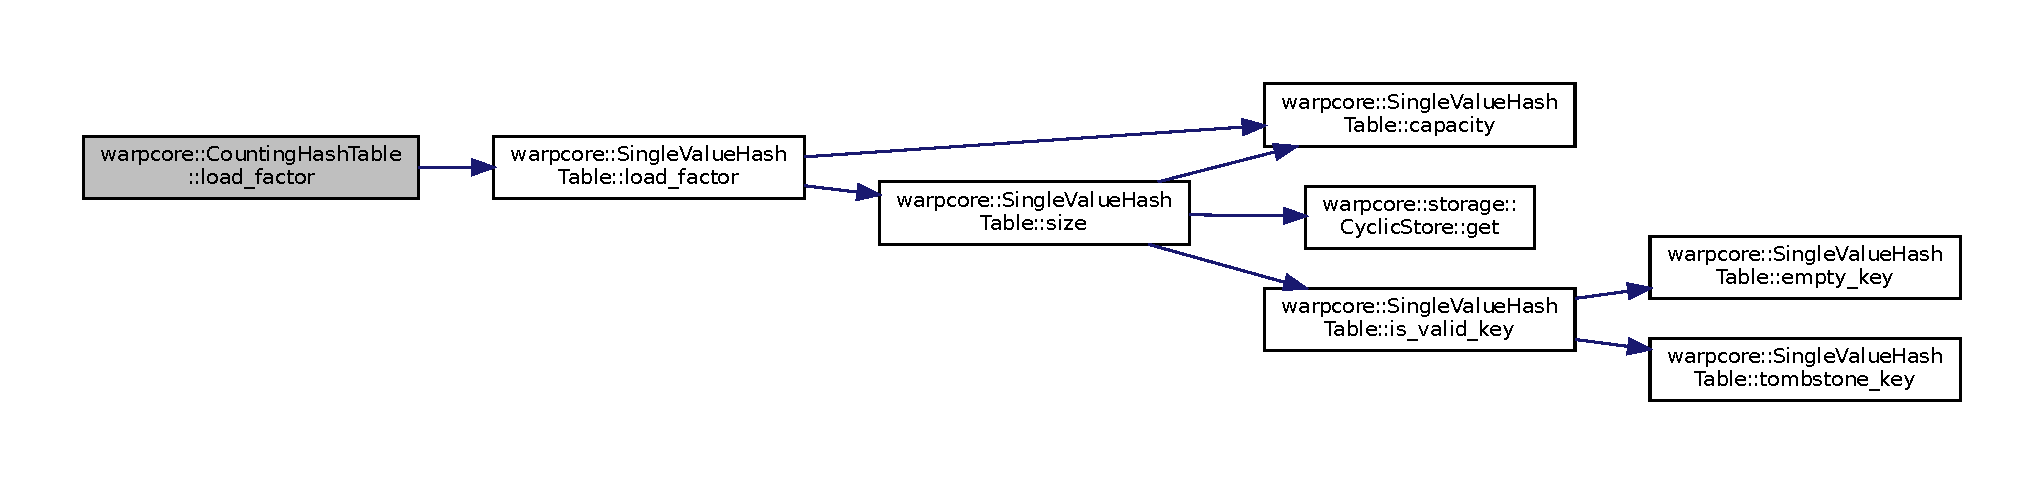
\includegraphics[width=350pt]{classwarpcore_1_1CountingHashTable_ad4a829b15a3add41133437c17ab6bf67_cgraph}
\end{center}
\end{figure}
\mbox{\Hypertarget{classwarpcore_1_1CountingHashTable_ae9e388f29dae1952c2da7fed32415e35}\label{classwarpcore_1_1CountingHashTable_ae9e388f29dae1952c2da7fed32415e35}} 
\index{warpcore::CountingHashTable$<$ Key, Value, EmptyKey, TombstoneKey, ProbingScheme, TableStorage, TempMemoryBytes $>$@{warpcore::CountingHashTable$<$ Key, Value, EmptyKey, TombstoneKey, ProbingScheme, TableStorage, TempMemoryBytes $>$}!peek\_status@{peek\_status}}
\index{peek\_status@{peek\_status}!warpcore::CountingHashTable$<$ Key, Value, EmptyKey, TombstoneKey, ProbingScheme, TableStorage, TempMemoryBytes $>$@{warpcore::CountingHashTable$<$ Key, Value, EmptyKey, TombstoneKey, ProbingScheme, TableStorage, TempMemoryBytes $>$}}
\doxysubsubsection{\texorpdfstring{peek\_status()}{peek\_status()}}
{\footnotesize\ttfamily template$<$class Key , class Value  = index\+\_\+t, Key Empty\+Key = defaults\+::empty\+\_\+key$<$\+Key$>$(), Key Tombstone\+Key = defaults\+::tombstone\+\_\+key$<$\+Key$>$(), class Probing\+Scheme  = defaults\+::probing\+\_\+scheme\+\_\+t$<$\+Key, 4$>$, class Table\+Storage  = defaults\+::table\+\_\+storage\+\_\+t$<$\+Key, Value$>$, index\+\_\+t Temp\+Memory\+Bytes = defaults\+::temp\+\_\+memory\+\_\+bytes()$>$ \\
\+\_\+\+\_\+host\+\_\+\+\_\+ status\+\_\+type \mbox{\hyperlink{classwarpcore_1_1CountingHashTable}{warpcore\+::\+Counting\+Hash\+Table}}$<$ Key, Value, Empty\+Key, Tombstone\+Key, Probing\+Scheme, Table\+Storage, Temp\+Memory\+Bytes $>$\+::peek\+\_\+status (\begin{DoxyParamCaption}\item[{cuda\+Stream\+\_\+t}]{stream = {\ttfamily 0} }\end{DoxyParamCaption}) const\hspace{0.3cm}{\ttfamily [inline]}, {\ttfamily [noexcept]}}



get the status of the hash table 


\begin{DoxyParams}{Parameters}
{\em stream} & C\+U\+DA stream in which this operation is executed in \\
\hline
\end{DoxyParams}
\begin{DoxyReturn}{Returns}
the status 
\end{DoxyReturn}
Here is the call graph for this function\+:
\nopagebreak
\begin{figure}[H]
\begin{center}
\leavevmode
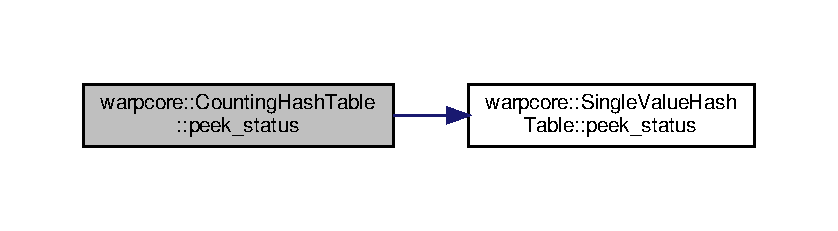
\includegraphics[width=350pt]{classwarpcore_1_1CountingHashTable_ae9e388f29dae1952c2da7fed32415e35_cgraph}
\end{center}
\end{figure}
\mbox{\Hypertarget{classwarpcore_1_1CountingHashTable_a9313aefeadf39f1c0512f131859922ab}\label{classwarpcore_1_1CountingHashTable_a9313aefeadf39f1c0512f131859922ab}} 
\index{warpcore::CountingHashTable$<$ Key, Value, EmptyKey, TombstoneKey, ProbingScheme, TableStorage, TempMemoryBytes $>$@{warpcore::CountingHashTable$<$ Key, Value, EmptyKey, TombstoneKey, ProbingScheme, TableStorage, TempMemoryBytes $>$}!pop\_status@{pop\_status}}
\index{pop\_status@{pop\_status}!warpcore::CountingHashTable$<$ Key, Value, EmptyKey, TombstoneKey, ProbingScheme, TableStorage, TempMemoryBytes $>$@{warpcore::CountingHashTable$<$ Key, Value, EmptyKey, TombstoneKey, ProbingScheme, TableStorage, TempMemoryBytes $>$}}
\doxysubsubsection{\texorpdfstring{pop\_status()}{pop\_status()}}
{\footnotesize\ttfamily template$<$class Key , class Value  = index\+\_\+t, Key Empty\+Key = defaults\+::empty\+\_\+key$<$\+Key$>$(), Key Tombstone\+Key = defaults\+::tombstone\+\_\+key$<$\+Key$>$(), class Probing\+Scheme  = defaults\+::probing\+\_\+scheme\+\_\+t$<$\+Key, 4$>$, class Table\+Storage  = defaults\+::table\+\_\+storage\+\_\+t$<$\+Key, Value$>$, index\+\_\+t Temp\+Memory\+Bytes = defaults\+::temp\+\_\+memory\+\_\+bytes()$>$ \\
\+\_\+\+\_\+host\+\_\+\+\_\+ status\+\_\+type \mbox{\hyperlink{classwarpcore_1_1CountingHashTable}{warpcore\+::\+Counting\+Hash\+Table}}$<$ Key, Value, Empty\+Key, Tombstone\+Key, Probing\+Scheme, Table\+Storage, Temp\+Memory\+Bytes $>$\+::pop\+\_\+status (\begin{DoxyParamCaption}\item[{cuda\+Stream\+\_\+t}]{stream = {\ttfamily 0} }\end{DoxyParamCaption})\hspace{0.3cm}{\ttfamily [inline]}, {\ttfamily [noexcept]}}



get and reset the status of the hash table 


\begin{DoxyParams}{Parameters}
{\em stream} & C\+U\+DA stream in which this operation is executed in \\
\hline
\end{DoxyParams}
\begin{DoxyReturn}{Returns}
the status 
\end{DoxyReturn}
Here is the call graph for this function\+:
\nopagebreak
\begin{figure}[H]
\begin{center}
\leavevmode
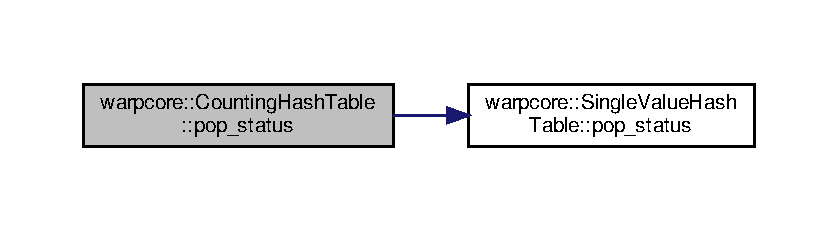
\includegraphics[width=350pt]{classwarpcore_1_1CountingHashTable_a9313aefeadf39f1c0512f131859922ab_cgraph}
\end{center}
\end{figure}
\mbox{\Hypertarget{classwarpcore_1_1CountingHashTable_a9abe12f3b4110a53e0cfc89a480a798f}\label{classwarpcore_1_1CountingHashTable_a9abe12f3b4110a53e0cfc89a480a798f}} 
\index{warpcore::CountingHashTable$<$ Key, Value, EmptyKey, TombstoneKey, ProbingScheme, TableStorage, TempMemoryBytes $>$@{warpcore::CountingHashTable$<$ Key, Value, EmptyKey, TombstoneKey, ProbingScheme, TableStorage, TempMemoryBytes $>$}!retrieve@{retrieve}}
\index{retrieve@{retrieve}!warpcore::CountingHashTable$<$ Key, Value, EmptyKey, TombstoneKey, ProbingScheme, TableStorage, TempMemoryBytes $>$@{warpcore::CountingHashTable$<$ Key, Value, EmptyKey, TombstoneKey, ProbingScheme, TableStorage, TempMemoryBytes $>$}}
\doxysubsubsection{\texorpdfstring{retrieve()}{retrieve()}\hspace{0.1cm}{\footnotesize\ttfamily [1/2]}}
{\footnotesize\ttfamily template$<$class Key , class Value  = index\+\_\+t, Key Empty\+Key = defaults\+::empty\+\_\+key$<$\+Key$>$(), Key Tombstone\+Key = defaults\+::tombstone\+\_\+key$<$\+Key$>$(), class Probing\+Scheme  = defaults\+::probing\+\_\+scheme\+\_\+t$<$\+Key, 4$>$, class Table\+Storage  = defaults\+::table\+\_\+storage\+\_\+t$<$\+Key, Value$>$, index\+\_\+t Temp\+Memory\+Bytes = defaults\+::temp\+\_\+memory\+\_\+bytes()$>$ \\
template$<$class Status\+Handler  = defaults\+::status\+\_\+handler\+\_\+t$>$ \\
\+\_\+\+\_\+host\+\_\+\+\_\+ void \mbox{\hyperlink{classwarpcore_1_1CountingHashTable}{warpcore\+::\+Counting\+Hash\+Table}}$<$ Key, Value, Empty\+Key, Tombstone\+Key, Probing\+Scheme, Table\+Storage, Temp\+Memory\+Bytes $>$\+::retrieve (\begin{DoxyParamCaption}\item[{key\+\_\+type $\ast$}]{keys\+\_\+in,  }\item[{index\+\_\+type}]{num\+\_\+in,  }\item[{value\+\_\+type $\ast$}]{values\+\_\+out,  }\item[{cuda\+Stream\+\_\+t}]{stream = {\ttfamily 0},  }\item[{index\+\_\+type}]{probing\+\_\+length = {\ttfamily defaults\+:\+:probing\+\_\+length()},  }\item[{typename Status\+Handler\+::base\+\_\+type $\ast$}]{status\+\_\+out = {\ttfamily nullptr} }\end{DoxyParamCaption}) const\hspace{0.3cm}{\ttfamily [inline]}, {\ttfamily [noexcept]}}



retrieve a set of keys from the hash table 


\begin{DoxyTemplParams}{Template Parameters}
{\em Status\+Handler} & handles status per key (see {\ttfamily \mbox{\hyperlink{namespacewarpcore_1_1status__handlers}{status\+\_\+handlers}}}) \\
\hline
\end{DoxyTemplParams}

\begin{DoxyParams}[1]{Parameters}
\mbox{\texttt{ in}}  & {\em keys\+\_\+in} & pointer to keys to retrieve from the hash table \\
\hline
\mbox{\texttt{ in}}  & {\em num\+\_\+in} & number of keys to retrieve \\
\hline
\mbox{\texttt{ out}}  & {\em values\+\_\+out} & corresponding counts of keys in {\ttfamily key\+\_\+in} \\
\hline
\mbox{\texttt{ in}}  & {\em stream} & C\+U\+DA stream in which this operation is executed in \\
\hline
\mbox{\texttt{ in}}  & {\em probing\+\_\+length} & maximum number of probing attempts \\
\hline
\mbox{\texttt{ out}}  & {\em status\+\_\+out} & status information (per key) \\
\hline
\end{DoxyParams}
Here is the call graph for this function\+:
\nopagebreak
\begin{figure}[H]
\begin{center}
\leavevmode
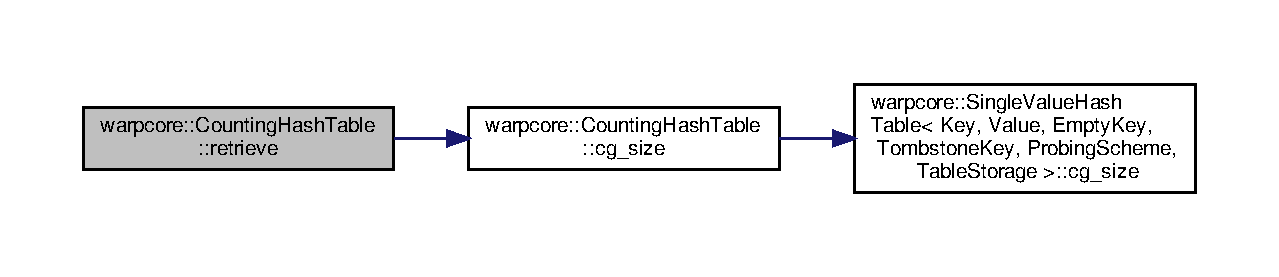
\includegraphics[width=350pt]{classwarpcore_1_1CountingHashTable_a9abe12f3b4110a53e0cfc89a480a798f_cgraph}
\end{center}
\end{figure}
\mbox{\Hypertarget{classwarpcore_1_1CountingHashTable_ab156b6726ca60e401fae990274b40cfc}\label{classwarpcore_1_1CountingHashTable_ab156b6726ca60e401fae990274b40cfc}} 
\index{warpcore::CountingHashTable$<$ Key, Value, EmptyKey, TombstoneKey, ProbingScheme, TableStorage, TempMemoryBytes $>$@{warpcore::CountingHashTable$<$ Key, Value, EmptyKey, TombstoneKey, ProbingScheme, TableStorage, TempMemoryBytes $>$}!retrieve@{retrieve}}
\index{retrieve@{retrieve}!warpcore::CountingHashTable$<$ Key, Value, EmptyKey, TombstoneKey, ProbingScheme, TableStorage, TempMemoryBytes $>$@{warpcore::CountingHashTable$<$ Key, Value, EmptyKey, TombstoneKey, ProbingScheme, TableStorage, TempMemoryBytes $>$}}
\doxysubsubsection{\texorpdfstring{retrieve()}{retrieve()}\hspace{0.1cm}{\footnotesize\ttfamily [2/2]}}
{\footnotesize\ttfamily template$<$class Key , class Value  = index\+\_\+t, Key Empty\+Key = defaults\+::empty\+\_\+key$<$\+Key$>$(), Key Tombstone\+Key = defaults\+::tombstone\+\_\+key$<$\+Key$>$(), class Probing\+Scheme  = defaults\+::probing\+\_\+scheme\+\_\+t$<$\+Key, 4$>$, class Table\+Storage  = defaults\+::table\+\_\+storage\+\_\+t$<$\+Key, Value$>$, index\+\_\+t Temp\+Memory\+Bytes = defaults\+::temp\+\_\+memory\+\_\+bytes()$>$ \\
\+\_\+\+\_\+device\+\_\+\+\_\+ status\+\_\+type \mbox{\hyperlink{classwarpcore_1_1CountingHashTable}{warpcore\+::\+Counting\+Hash\+Table}}$<$ Key, Value, Empty\+Key, Tombstone\+Key, Probing\+Scheme, Table\+Storage, Temp\+Memory\+Bytes $>$\+::retrieve (\begin{DoxyParamCaption}\item[{key\+\_\+type}]{key\+\_\+in,  }\item[{value\+\_\+type \&}]{value\+\_\+out,  }\item[{const cg\+::thread\+\_\+block\+\_\+tile$<$ \mbox{\hyperlink{classwarpcore_1_1CountingHashTable_a5efe6f4060321596322a99a28fcaef93}{cg\+\_\+size}}()$>$ \&}]{group,  }\item[{index\+\_\+type}]{probing\+\_\+length = {\ttfamily defaults\+:\+:probing\+\_\+length()} }\end{DoxyParamCaption}) const\hspace{0.3cm}{\ttfamily [inline]}, {\ttfamily [noexcept]}}



retrieves a key from the hash table 


\begin{DoxyParams}[1]{Parameters}
\mbox{\texttt{ in}}  & {\em key\+\_\+in} & key to retrieve from the hash table \\
\hline
\mbox{\texttt{ out}}  & {\em value\+\_\+out} & count of {\ttfamily key\+\_\+in} \\
\hline
\mbox{\texttt{ in}}  & {\em group} & cooperative group \\
\hline
\mbox{\texttt{ in}}  & {\em probing\+\_\+length} & maximum number of probing attempts \\
\hline
\end{DoxyParams}
\begin{DoxyReturn}{Returns}
status (per thread) 
\end{DoxyReturn}
Here is the call graph for this function\+:
\nopagebreak
\begin{figure}[H]
\begin{center}
\leavevmode
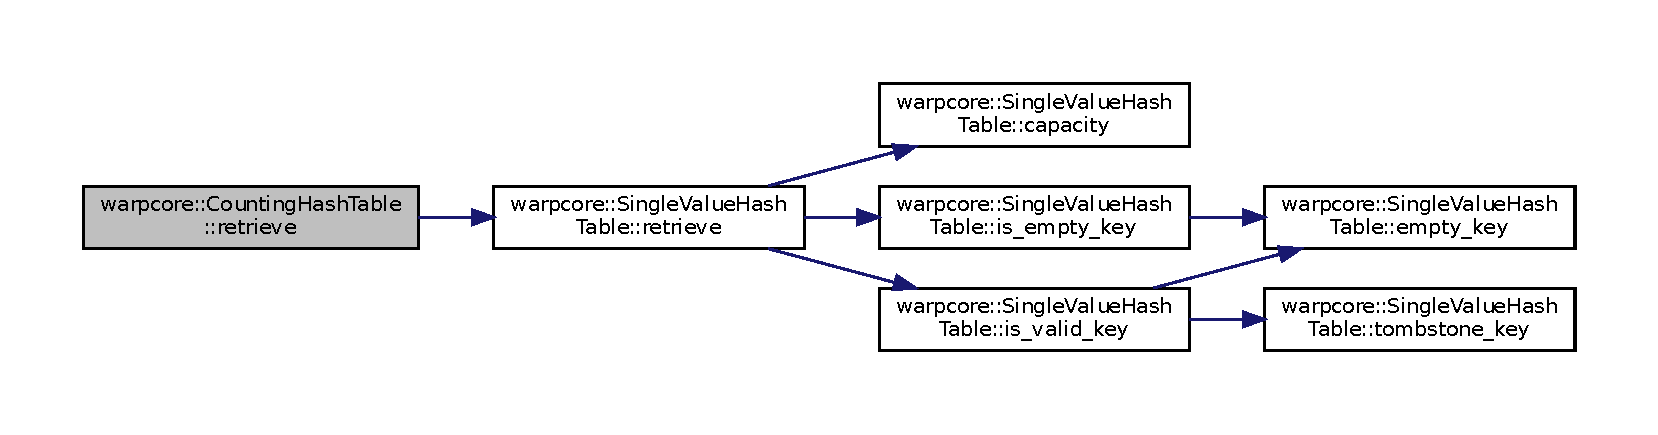
\includegraphics[width=350pt]{classwarpcore_1_1CountingHashTable_ab156b6726ca60e401fae990274b40cfc_cgraph}
\end{center}
\end{figure}
\mbox{\Hypertarget{classwarpcore_1_1CountingHashTable_aade49f5de5f2144d57cdcfe8b7ad6663}\label{classwarpcore_1_1CountingHashTable_aade49f5de5f2144d57cdcfe8b7ad6663}} 
\index{warpcore::CountingHashTable$<$ Key, Value, EmptyKey, TombstoneKey, ProbingScheme, TableStorage, TempMemoryBytes $>$@{warpcore::CountingHashTable$<$ Key, Value, EmptyKey, TombstoneKey, ProbingScheme, TableStorage, TempMemoryBytes $>$}!retrieve\_all@{retrieve\_all}}
\index{retrieve\_all@{retrieve\_all}!warpcore::CountingHashTable$<$ Key, Value, EmptyKey, TombstoneKey, ProbingScheme, TableStorage, TempMemoryBytes $>$@{warpcore::CountingHashTable$<$ Key, Value, EmptyKey, TombstoneKey, ProbingScheme, TableStorage, TempMemoryBytes $>$}}
\doxysubsubsection{\texorpdfstring{retrieve\_all()}{retrieve\_all()}}
{\footnotesize\ttfamily template$<$class Key , class Value  = index\+\_\+t, Key Empty\+Key = defaults\+::empty\+\_\+key$<$\+Key$>$(), Key Tombstone\+Key = defaults\+::tombstone\+\_\+key$<$\+Key$>$(), class Probing\+Scheme  = defaults\+::probing\+\_\+scheme\+\_\+t$<$\+Key, 4$>$, class Table\+Storage  = defaults\+::table\+\_\+storage\+\_\+t$<$\+Key, Value$>$, index\+\_\+t Temp\+Memory\+Bytes = defaults\+::temp\+\_\+memory\+\_\+bytes()$>$ \\
\+\_\+\+\_\+host\+\_\+\+\_\+ void \mbox{\hyperlink{classwarpcore_1_1CountingHashTable}{warpcore\+::\+Counting\+Hash\+Table}}$<$ Key, Value, Empty\+Key, Tombstone\+Key, Probing\+Scheme, Table\+Storage, Temp\+Memory\+Bytes $>$\+::retrieve\+\_\+all (\begin{DoxyParamCaption}\item[{key\+\_\+type $\ast$}]{keys\+\_\+out,  }\item[{value\+\_\+type $\ast$}]{values\+\_\+out,  }\item[{index\+\_\+t \&}]{num\+\_\+out,  }\item[{cuda\+Stream\+\_\+t}]{stream = {\ttfamily 0} }\end{DoxyParamCaption}) const\hspace{0.3cm}{\ttfamily [inline]}, {\ttfamily [noexcept]}}



retrieves all elements from the hash table 


\begin{DoxyParams}[1]{Parameters}
\mbox{\texttt{ out}}  & {\em keys\+\_\+out} & location to store all retrieved keys \\
\hline
\mbox{\texttt{ out}}  & {\em values\+\_\+out} & location to store all retrieved counts \\
\hline
\mbox{\texttt{ out}}  & {\em num\+\_\+out} & number of of key/value pairs retrieved \\
\hline
\mbox{\texttt{ in}}  & {\em stream} & C\+U\+DA stream in which this operation is executed in \\
\hline
\end{DoxyParams}
Here is the call graph for this function\+:
\nopagebreak
\begin{figure}[H]
\begin{center}
\leavevmode
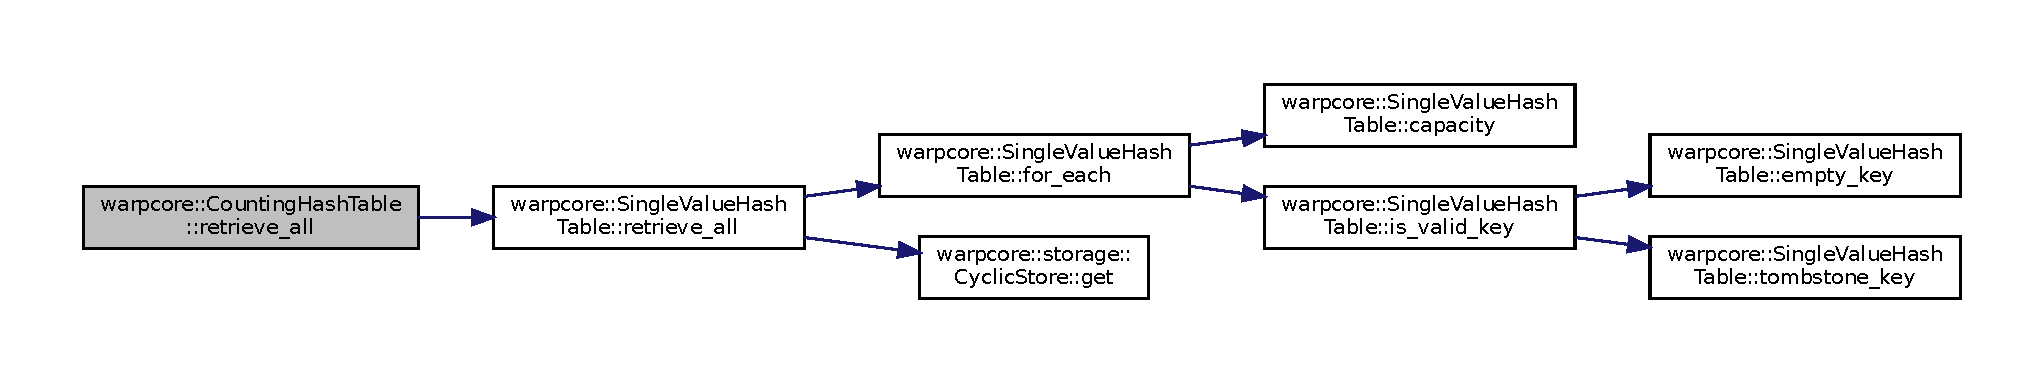
\includegraphics[width=350pt]{classwarpcore_1_1CountingHashTable_aade49f5de5f2144d57cdcfe8b7ad6663_cgraph}
\end{center}
\end{figure}
\mbox{\Hypertarget{classwarpcore_1_1CountingHashTable_a404f39442f096f294cd879b0710e5416}\label{classwarpcore_1_1CountingHashTable_a404f39442f096f294cd879b0710e5416}} 
\index{warpcore::CountingHashTable$<$ Key, Value, EmptyKey, TombstoneKey, ProbingScheme, TableStorage, TempMemoryBytes $>$@{warpcore::CountingHashTable$<$ Key, Value, EmptyKey, TombstoneKey, ProbingScheme, TableStorage, TempMemoryBytes $>$}!seed@{seed}}
\index{seed@{seed}!warpcore::CountingHashTable$<$ Key, Value, EmptyKey, TombstoneKey, ProbingScheme, TableStorage, TempMemoryBytes $>$@{warpcore::CountingHashTable$<$ Key, Value, EmptyKey, TombstoneKey, ProbingScheme, TableStorage, TempMemoryBytes $>$}}
\doxysubsubsection{\texorpdfstring{seed()}{seed()}}
{\footnotesize\ttfamily template$<$class Key , class Value  = index\+\_\+t, Key Empty\+Key = defaults\+::empty\+\_\+key$<$\+Key$>$(), Key Tombstone\+Key = defaults\+::tombstone\+\_\+key$<$\+Key$>$(), class Probing\+Scheme  = defaults\+::probing\+\_\+scheme\+\_\+t$<$\+Key, 4$>$, class Table\+Storage  = defaults\+::table\+\_\+storage\+\_\+t$<$\+Key, Value$>$, index\+\_\+t Temp\+Memory\+Bytes = defaults\+::temp\+\_\+memory\+\_\+bytes()$>$ \\
\+\_\+\+\_\+host\+\_\+\+\_\+\+\_\+\+\_\+device\+\_\+\+\_\+ key\+\_\+type \mbox{\hyperlink{classwarpcore_1_1CountingHashTable}{warpcore\+::\+Counting\+Hash\+Table}}$<$ Key, Value, Empty\+Key, Tombstone\+Key, Probing\+Scheme, Table\+Storage, Temp\+Memory\+Bytes $>$\+::seed (\begin{DoxyParamCaption}{ }\end{DoxyParamCaption}) const\hspace{0.3cm}{\ttfamily [inline]}, {\ttfamily [noexcept]}}



get random seed 

\begin{DoxyReturn}{Returns}
seed 
\end{DoxyReturn}
Here is the call graph for this function\+:
\nopagebreak
\begin{figure}[H]
\begin{center}
\leavevmode
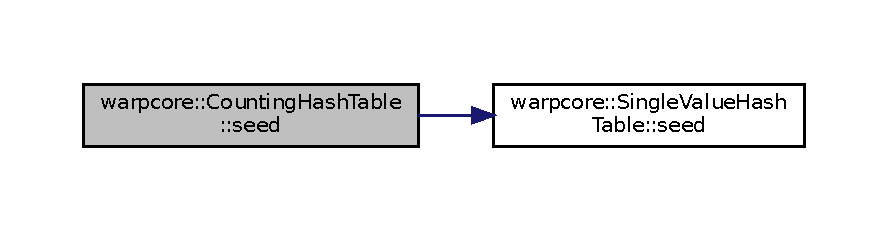
\includegraphics[width=350pt]{classwarpcore_1_1CountingHashTable_a404f39442f096f294cd879b0710e5416_cgraph}
\end{center}
\end{figure}
Here is the caller graph for this function\+:
\nopagebreak
\begin{figure}[H]
\begin{center}
\leavevmode
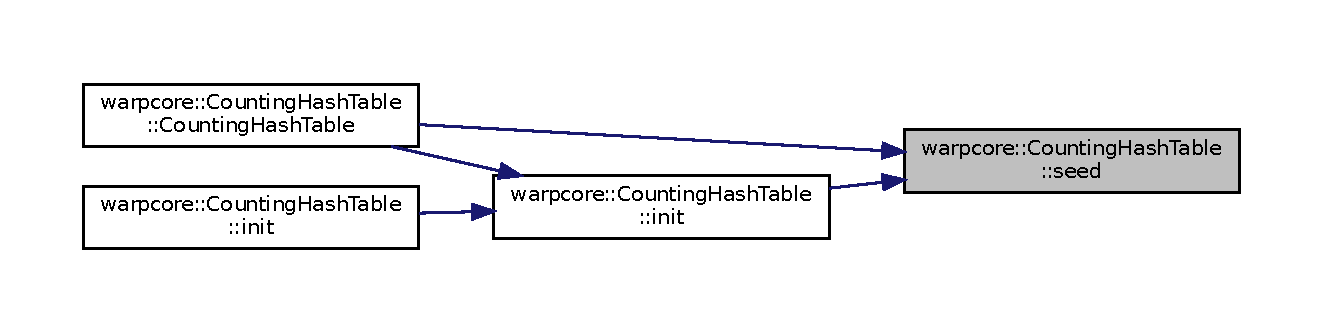
\includegraphics[width=350pt]{classwarpcore_1_1CountingHashTable_a404f39442f096f294cd879b0710e5416_icgraph}
\end{center}
\end{figure}
\mbox{\Hypertarget{classwarpcore_1_1CountingHashTable_aa331f755c38f5b073ed7e58e3ad59777}\label{classwarpcore_1_1CountingHashTable_aa331f755c38f5b073ed7e58e3ad59777}} 
\index{warpcore::CountingHashTable$<$ Key, Value, EmptyKey, TombstoneKey, ProbingScheme, TableStorage, TempMemoryBytes $>$@{warpcore::CountingHashTable$<$ Key, Value, EmptyKey, TombstoneKey, ProbingScheme, TableStorage, TempMemoryBytes $>$}!size@{size}}
\index{size@{size}!warpcore::CountingHashTable$<$ Key, Value, EmptyKey, TombstoneKey, ProbingScheme, TableStorage, TempMemoryBytes $>$@{warpcore::CountingHashTable$<$ Key, Value, EmptyKey, TombstoneKey, ProbingScheme, TableStorage, TempMemoryBytes $>$}}
\doxysubsubsection{\texorpdfstring{size()}{size()}}
{\footnotesize\ttfamily template$<$class Key , class Value  = index\+\_\+t, Key Empty\+Key = defaults\+::empty\+\_\+key$<$\+Key$>$(), Key Tombstone\+Key = defaults\+::tombstone\+\_\+key$<$\+Key$>$(), class Probing\+Scheme  = defaults\+::probing\+\_\+scheme\+\_\+t$<$\+Key, 4$>$, class Table\+Storage  = defaults\+::table\+\_\+storage\+\_\+t$<$\+Key, Value$>$, index\+\_\+t Temp\+Memory\+Bytes = defaults\+::temp\+\_\+memory\+\_\+bytes()$>$ \\
\+\_\+\+\_\+host\+\_\+\+\_\+ index\+\_\+type \mbox{\hyperlink{classwarpcore_1_1CountingHashTable}{warpcore\+::\+Counting\+Hash\+Table}}$<$ Key, Value, Empty\+Key, Tombstone\+Key, Probing\+Scheme, Table\+Storage, Temp\+Memory\+Bytes $>$\+::size (\begin{DoxyParamCaption}\item[{cuda\+Stream\+\_\+t}]{stream = {\ttfamily 0} }\end{DoxyParamCaption}) const\hspace{0.3cm}{\ttfamily [inline]}, {\ttfamily [noexcept]}}



number of key/value pairs stored inside the hash table 


\begin{DoxyParams}{Parameters}
{\em stream} & C\+U\+DA stream in which this operation is executed in \\
\hline
\end{DoxyParams}
\begin{DoxyReturn}{Returns}
the number of key/value pairs inside the hash table 
\end{DoxyReturn}
Here is the call graph for this function\+:
\nopagebreak
\begin{figure}[H]
\begin{center}
\leavevmode
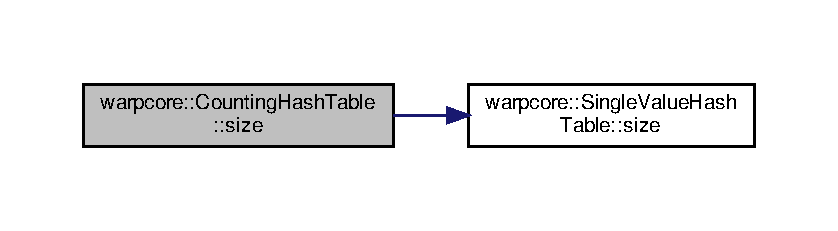
\includegraphics[width=350pt]{classwarpcore_1_1CountingHashTable_aa331f755c38f5b073ed7e58e3ad59777_cgraph}
\end{center}
\end{figure}
\mbox{\Hypertarget{classwarpcore_1_1CountingHashTable_aa7b5b49d50edc280ce007cf92abdc4ae}\label{classwarpcore_1_1CountingHashTable_aa7b5b49d50edc280ce007cf92abdc4ae}} 
\index{warpcore::CountingHashTable$<$ Key, Value, EmptyKey, TombstoneKey, ProbingScheme, TableStorage, TempMemoryBytes $>$@{warpcore::CountingHashTable$<$ Key, Value, EmptyKey, TombstoneKey, ProbingScheme, TableStorage, TempMemoryBytes $>$}!storage\_density@{storage\_density}}
\index{storage\_density@{storage\_density}!warpcore::CountingHashTable$<$ Key, Value, EmptyKey, TombstoneKey, ProbingScheme, TableStorage, TempMemoryBytes $>$@{warpcore::CountingHashTable$<$ Key, Value, EmptyKey, TombstoneKey, ProbingScheme, TableStorage, TempMemoryBytes $>$}}
\doxysubsubsection{\texorpdfstring{storage\_density()}{storage\_density()}}
{\footnotesize\ttfamily template$<$class Key , class Value  = index\+\_\+t, Key Empty\+Key = defaults\+::empty\+\_\+key$<$\+Key$>$(), Key Tombstone\+Key = defaults\+::tombstone\+\_\+key$<$\+Key$>$(), class Probing\+Scheme  = defaults\+::probing\+\_\+scheme\+\_\+t$<$\+Key, 4$>$, class Table\+Storage  = defaults\+::table\+\_\+storage\+\_\+t$<$\+Key, Value$>$, index\+\_\+t Temp\+Memory\+Bytes = defaults\+::temp\+\_\+memory\+\_\+bytes()$>$ \\
\+\_\+\+\_\+host\+\_\+\+\_\+ float \mbox{\hyperlink{classwarpcore_1_1CountingHashTable}{warpcore\+::\+Counting\+Hash\+Table}}$<$ Key, Value, Empty\+Key, Tombstone\+Key, Probing\+Scheme, Table\+Storage, Temp\+Memory\+Bytes $>$\+::storage\+\_\+density (\begin{DoxyParamCaption}\item[{cuda\+Stream\+\_\+t}]{stream = {\ttfamily 0} }\end{DoxyParamCaption}) const\hspace{0.3cm}{\ttfamily [inline]}, {\ttfamily [noexcept]}}



current storage density of the hash table 


\begin{DoxyParams}{Parameters}
{\em stream} & C\+U\+DA stream in which this operation is executed in \\
\hline
\end{DoxyParams}
\begin{DoxyReturn}{Returns}
storage density 
\end{DoxyReturn}
Here is the call graph for this function\+:
\nopagebreak
\begin{figure}[H]
\begin{center}
\leavevmode
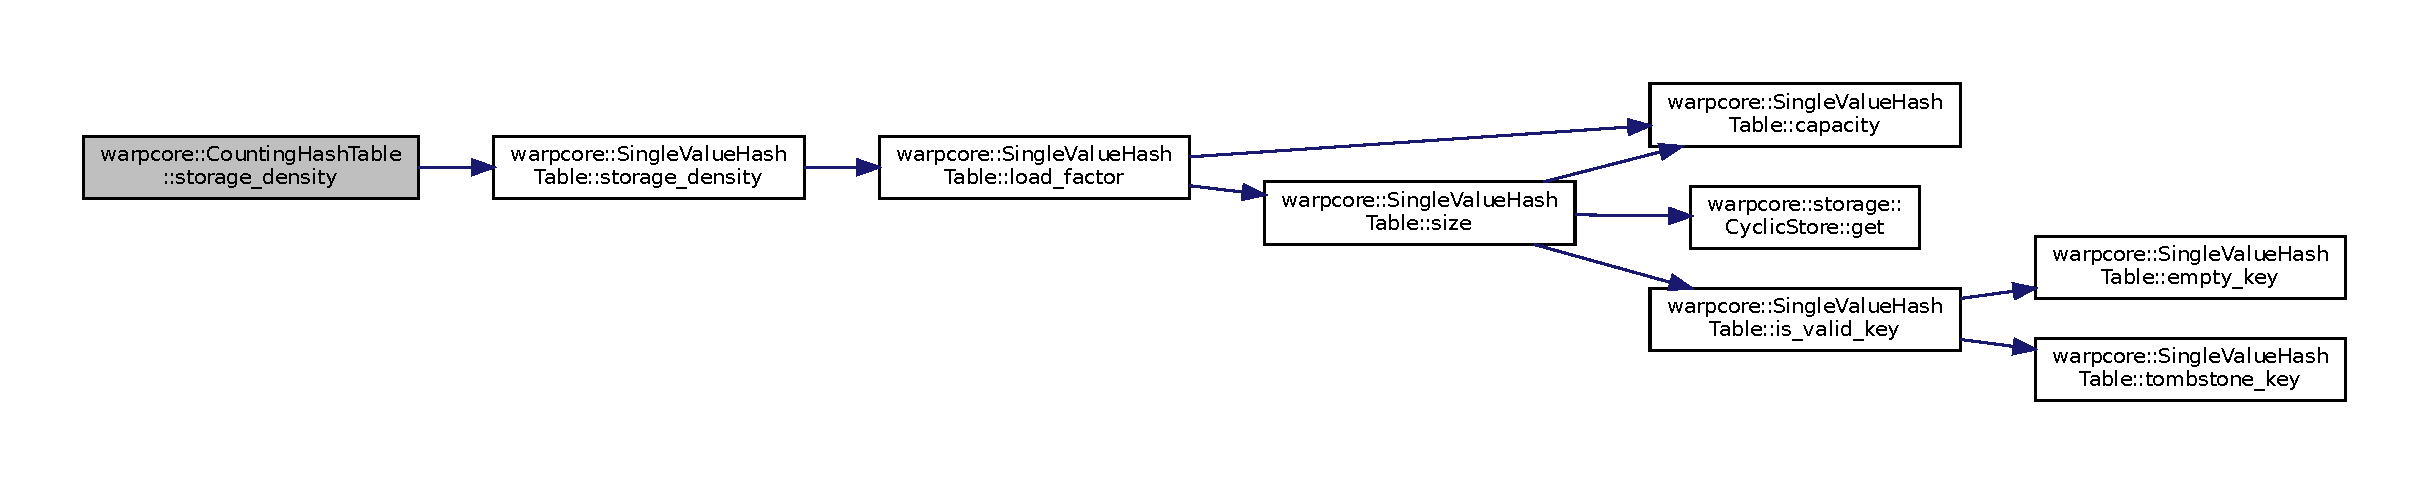
\includegraphics[width=350pt]{classwarpcore_1_1CountingHashTable_aa7b5b49d50edc280ce007cf92abdc4ae_cgraph}
\end{center}
\end{figure}
\mbox{\Hypertarget{classwarpcore_1_1CountingHashTable_a742dcef5845153aacbf6d8790a5f0fac}\label{classwarpcore_1_1CountingHashTable_a742dcef5845153aacbf6d8790a5f0fac}} 
\index{warpcore::CountingHashTable$<$ Key, Value, EmptyKey, TombstoneKey, ProbingScheme, TableStorage, TempMemoryBytes $>$@{warpcore::CountingHashTable$<$ Key, Value, EmptyKey, TombstoneKey, ProbingScheme, TableStorage, TempMemoryBytes $>$}!tombstone\_key@{tombstone\_key}}
\index{tombstone\_key@{tombstone\_key}!warpcore::CountingHashTable$<$ Key, Value, EmptyKey, TombstoneKey, ProbingScheme, TableStorage, TempMemoryBytes $>$@{warpcore::CountingHashTable$<$ Key, Value, EmptyKey, TombstoneKey, ProbingScheme, TableStorage, TempMemoryBytes $>$}}
\doxysubsubsection{\texorpdfstring{tombstone\_key()}{tombstone\_key()}}
{\footnotesize\ttfamily template$<$class Key , class Value  = index\+\_\+t, Key Empty\+Key = defaults\+::empty\+\_\+key$<$\+Key$>$(), Key Tombstone\+Key = defaults\+::tombstone\+\_\+key$<$\+Key$>$(), class Probing\+Scheme  = defaults\+::probing\+\_\+scheme\+\_\+t$<$\+Key, 4$>$, class Table\+Storage  = defaults\+::table\+\_\+storage\+\_\+t$<$\+Key, Value$>$, index\+\_\+t Temp\+Memory\+Bytes = defaults\+::temp\+\_\+memory\+\_\+bytes()$>$ \\
static constexpr \+\_\+\+\_\+host\+\_\+\+\_\+\+\_\+\+\_\+device\+\_\+\+\_\+ key\+\_\+type \mbox{\hyperlink{classwarpcore_1_1CountingHashTable}{warpcore\+::\+Counting\+Hash\+Table}}$<$ Key, Value, Empty\+Key, Tombstone\+Key, Probing\+Scheme, Table\+Storage, Temp\+Memory\+Bytes $>$\+::tombstone\+\_\+key (\begin{DoxyParamCaption}{ }\end{DoxyParamCaption})\hspace{0.3cm}{\ttfamily [inline]}, {\ttfamily [static]}, {\ttfamily [constexpr]}, {\ttfamily [noexcept]}}



get tombstone key 

\begin{DoxyReturn}{Returns}
tombstone key 
\end{DoxyReturn}
Here is the call graph for this function\+:
\nopagebreak
\begin{figure}[H]
\begin{center}
\leavevmode
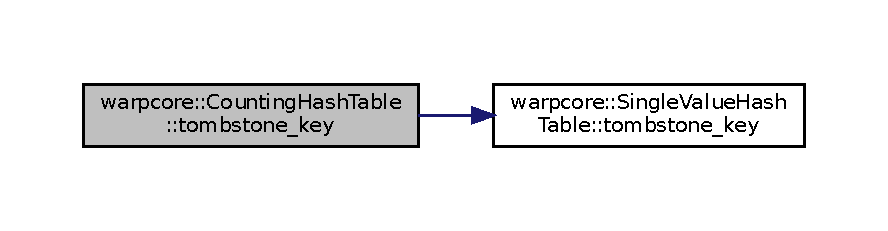
\includegraphics[width=350pt]{classwarpcore_1_1CountingHashTable_a742dcef5845153aacbf6d8790a5f0fac_cgraph}
\end{center}
\end{figure}

\hypertarget{classwarpcore_1_1storage_1_1CyclicStore}{}\section{warpcore\+:\+:storage\+:\+:Cyclic\+Store$<$ T $>$ Class Template Reference}
\label{classwarpcore_1_1storage_1_1CyclicStore}\index{warpcore\+::storage\+::\+Cyclic\+Store$<$ T $>$@{warpcore\+::storage\+::\+Cyclic\+Store$<$ T $>$}}


thread-\/safe device-\/sided ring buffer without any overflow checks  




Inheritance diagram for warpcore\+:\+:storage\+:\+:Cyclic\+Store$<$ T $>$\+:
\nopagebreak
\begin{figure}[H]
\begin{center}
\leavevmode
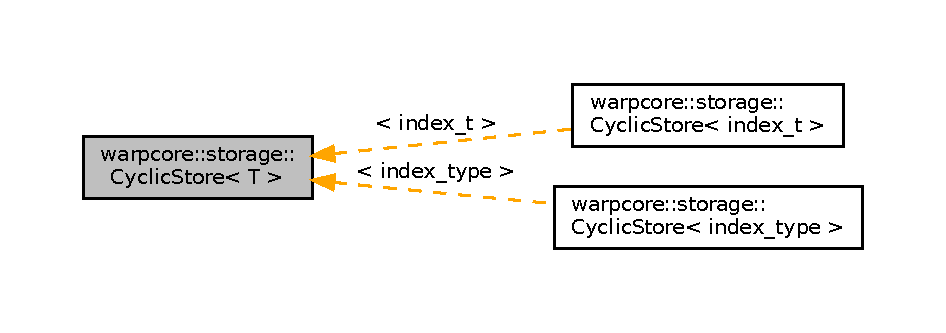
\includegraphics[width=350pt]{classwarpcore_1_1storage_1_1CyclicStore__inherit__graph}
\end{center}
\end{figure}
\subsection*{Public Types}
\begin{DoxyCompactItemize}
\item 
\mbox{\Hypertarget{classwarpcore_1_1storage_1_1CyclicStore_aab3dd4b7cf7aa2ec39bdd0abf33fc7aa}\label{classwarpcore_1_1storage_1_1CyclicStore_aab3dd4b7cf7aa2ec39bdd0abf33fc7aa}} 
using {\bfseries base\+\_\+type} = T
\item 
\mbox{\Hypertarget{classwarpcore_1_1storage_1_1CyclicStore_ad87f57968d5eb91a7fa7eb2ee69738d5}\label{classwarpcore_1_1storage_1_1CyclicStore_ad87f57968d5eb91a7fa7eb2ee69738d5}} 
using {\bfseries index\+\_\+type} = index\+\_\+t
\item 
\mbox{\Hypertarget{classwarpcore_1_1storage_1_1CyclicStore_a83b3e0937acd2dcb0c61297ca142a482}\label{classwarpcore_1_1storage_1_1CyclicStore_a83b3e0937acd2dcb0c61297ca142a482}} 
using {\bfseries status\+\_\+type} = \hyperlink{classwarpcore_1_1Status}{Status}
\end{DoxyCompactItemize}
\subsection*{Public Member Functions}
\begin{DoxyCompactItemize}
\item 
\+\_\+\+\_\+host\+\_\+\+\_\+ \hyperlink{classwarpcore_1_1storage_1_1CyclicStore_aca834b00d59e653c092db712ca7eb7a0}{Cyclic\+Store} (const index\+\_\+type \hyperlink{classwarpcore_1_1storage_1_1CyclicStore_acc4bfbb9b10868a193301d0ec5a46711}{capacity}) noexcept
\begin{DoxyCompactList}\small\item\em constructor \end{DoxyCompactList}\item 
\+\_\+\+\_\+host\+\_\+\+\_\+\+\_\+\+\_\+device\+\_\+\+\_\+ \hyperlink{classwarpcore_1_1storage_1_1CyclicStore_a8c9f9193f3a45063b9b73fece142aa81}{Cyclic\+Store} (const \hyperlink{classwarpcore_1_1storage_1_1CyclicStore}{Cyclic\+Store} \&o) noexcept
\begin{DoxyCompactList}\small\item\em copy-\/constructor (shallow) \end{DoxyCompactList}\item 
\+\_\+\+\_\+host\+\_\+\+\_\+ \hyperlink{classwarpcore_1_1storage_1_1CyclicStore_a5657f1b2e0f9f7c8ee0de28d2c305cf0}{Cyclic\+Store} (\hyperlink{classwarpcore_1_1storage_1_1CyclicStore}{Cyclic\+Store} \&\&o) noexcept
\begin{DoxyCompactList}\small\item\em move-\/constructor \end{DoxyCompactList}\item 
\mbox{\Hypertarget{classwarpcore_1_1storage_1_1CyclicStore_a4ccee1383c1d6434c49fae48a1e6c9c0}\label{classwarpcore_1_1storage_1_1CyclicStore_a4ccee1383c1d6434c49fae48a1e6c9c0}} 
\+\_\+\+\_\+host\+\_\+\+\_\+ \hyperlink{classwarpcore_1_1storage_1_1CyclicStore_a4ccee1383c1d6434c49fae48a1e6c9c0}{$\sim$\+Cyclic\+Store} () noexcept
\begin{DoxyCompactList}\small\item\em destructor \end{DoxyCompactList}\item 
\+\_\+\+\_\+host\+\_\+\+\_\+ T $\ast$ \hyperlink{classwarpcore_1_1storage_1_1CyclicStore_ab475e047f32b8a8358ea6b78dfe2536d}{get} () const noexcept
\begin{DoxyCompactList}\small\item\em atomically fetches the next slot in the buffer \end{DoxyCompactList}\item 
\+\_\+\+\_\+host\+\_\+\+\_\+ \hyperlink{classwarpcore_1_1Status}{status\+\_\+type} \hyperlink{classwarpcore_1_1storage_1_1CyclicStore_ab6c224b2b5a49d93dc7e052ec7b8cc32}{status} () const noexcept
\begin{DoxyCompactList}\small\item\em get buffer status \end{DoxyCompactList}\item 
\+\_\+\+\_\+host\+\_\+\+\_\+ index\+\_\+type \hyperlink{classwarpcore_1_1storage_1_1CyclicStore_acc4bfbb9b10868a193301d0ec5a46711}{capacity} () const noexcept
\begin{DoxyCompactList}\small\item\em get buffer capacity \end{DoxyCompactList}\item 
\+\_\+\+\_\+host\+\_\+\+\_\+ index\+\_\+type \hyperlink{classwarpcore_1_1storage_1_1CyclicStore_ae65e099d0cfe170fc4cd2f02682c3bda}{bytes\+\_\+total} () const noexcept
\begin{DoxyCompactList}\small\item\em get the total number of bytes occupied by this data structure \end{DoxyCompactList}\end{DoxyCompactItemize}


\subsection{Detailed Description}
\subsubsection*{template$<$class T$>$\newline
class warpcore\+::storage\+::\+Cyclic\+Store$<$ T $>$}

thread-\/safe device-\/sided ring buffer without any overflow checks 


\begin{DoxyTemplParams}{Template Parameters}
{\em T} & base type \\
\hline
\end{DoxyTemplParams}


\subsection{Constructor \& Destructor Documentation}
\mbox{\Hypertarget{classwarpcore_1_1storage_1_1CyclicStore_aca834b00d59e653c092db712ca7eb7a0}\label{classwarpcore_1_1storage_1_1CyclicStore_aca834b00d59e653c092db712ca7eb7a0}} 
\index{warpcore\+::storage\+::\+Cyclic\+Store@{warpcore\+::storage\+::\+Cyclic\+Store}!Cyclic\+Store@{Cyclic\+Store}}
\index{Cyclic\+Store@{Cyclic\+Store}!warpcore\+::storage\+::\+Cyclic\+Store@{warpcore\+::storage\+::\+Cyclic\+Store}}
\subsubsection{\texorpdfstring{Cyclic\+Store()}{CyclicStore()}\hspace{0.1cm}{\footnotesize\ttfamily [1/3]}}
{\footnotesize\ttfamily template$<$class T$>$ \\
\+\_\+\+\_\+host\+\_\+\+\_\+ \hyperlink{classwarpcore_1_1storage_1_1CyclicStore}{warpcore\+::storage\+::\+Cyclic\+Store}$<$ T $>$\+::\hyperlink{classwarpcore_1_1storage_1_1CyclicStore}{Cyclic\+Store} (\begin{DoxyParamCaption}\item[{const index\+\_\+type}]{capacity }\end{DoxyParamCaption})\hspace{0.3cm}{\ttfamily [inline]}, {\ttfamily [explicit]}, {\ttfamily [noexcept]}}



constructor 


\begin{DoxyParams}[1]{Parameters}
\mbox{\tt in}  & {\em capacity} & buffer capacity \\
\hline
\end{DoxyParams}
\mbox{\Hypertarget{classwarpcore_1_1storage_1_1CyclicStore_a8c9f9193f3a45063b9b73fece142aa81}\label{classwarpcore_1_1storage_1_1CyclicStore_a8c9f9193f3a45063b9b73fece142aa81}} 
\index{warpcore\+::storage\+::\+Cyclic\+Store@{warpcore\+::storage\+::\+Cyclic\+Store}!Cyclic\+Store@{Cyclic\+Store}}
\index{Cyclic\+Store@{Cyclic\+Store}!warpcore\+::storage\+::\+Cyclic\+Store@{warpcore\+::storage\+::\+Cyclic\+Store}}
\subsubsection{\texorpdfstring{Cyclic\+Store()}{CyclicStore()}\hspace{0.1cm}{\footnotesize\ttfamily [2/3]}}
{\footnotesize\ttfamily template$<$class T$>$ \\
\+\_\+\+\_\+host\+\_\+\+\_\+\+\_\+\+\_\+device\+\_\+\+\_\+ \hyperlink{classwarpcore_1_1storage_1_1CyclicStore}{warpcore\+::storage\+::\+Cyclic\+Store}$<$ T $>$\+::\hyperlink{classwarpcore_1_1storage_1_1CyclicStore}{Cyclic\+Store} (\begin{DoxyParamCaption}\item[{const \hyperlink{classwarpcore_1_1storage_1_1CyclicStore}{Cyclic\+Store}$<$ T $>$ \&}]{o }\end{DoxyParamCaption})\hspace{0.3cm}{\ttfamily [inline]}, {\ttfamily [noexcept]}}



copy-\/constructor (shallow) 


\begin{DoxyParams}[1]{Parameters}
\mbox{\tt in}  & {\em object} & to be copied \\
\hline
\end{DoxyParams}
\mbox{\Hypertarget{classwarpcore_1_1storage_1_1CyclicStore_a5657f1b2e0f9f7c8ee0de28d2c305cf0}\label{classwarpcore_1_1storage_1_1CyclicStore_a5657f1b2e0f9f7c8ee0de28d2c305cf0}} 
\index{warpcore\+::storage\+::\+Cyclic\+Store@{warpcore\+::storage\+::\+Cyclic\+Store}!Cyclic\+Store@{Cyclic\+Store}}
\index{Cyclic\+Store@{Cyclic\+Store}!warpcore\+::storage\+::\+Cyclic\+Store@{warpcore\+::storage\+::\+Cyclic\+Store}}
\subsubsection{\texorpdfstring{Cyclic\+Store()}{CyclicStore()}\hspace{0.1cm}{\footnotesize\ttfamily [3/3]}}
{\footnotesize\ttfamily template$<$class T$>$ \\
\+\_\+\+\_\+host\+\_\+\+\_\+ \hyperlink{classwarpcore_1_1storage_1_1CyclicStore}{warpcore\+::storage\+::\+Cyclic\+Store}$<$ T $>$\+::\hyperlink{classwarpcore_1_1storage_1_1CyclicStore}{Cyclic\+Store} (\begin{DoxyParamCaption}\item[{\hyperlink{classwarpcore_1_1storage_1_1CyclicStore}{Cyclic\+Store}$<$ T $>$ \&\&}]{o }\end{DoxyParamCaption})\hspace{0.3cm}{\ttfamily [inline]}, {\ttfamily [noexcept]}}



move-\/constructor 


\begin{DoxyParams}[1]{Parameters}
\mbox{\tt in}  & {\em object} & to be moved \\
\hline
\end{DoxyParams}


\subsection{Member Function Documentation}
\mbox{\Hypertarget{classwarpcore_1_1storage_1_1CyclicStore_ae65e099d0cfe170fc4cd2f02682c3bda}\label{classwarpcore_1_1storage_1_1CyclicStore_ae65e099d0cfe170fc4cd2f02682c3bda}} 
\index{warpcore\+::storage\+::\+Cyclic\+Store@{warpcore\+::storage\+::\+Cyclic\+Store}!bytes\+\_\+total@{bytes\+\_\+total}}
\index{bytes\+\_\+total@{bytes\+\_\+total}!warpcore\+::storage\+::\+Cyclic\+Store@{warpcore\+::storage\+::\+Cyclic\+Store}}
\subsubsection{\texorpdfstring{bytes\+\_\+total()}{bytes\_total()}}
{\footnotesize\ttfamily template$<$class T$>$ \\
\+\_\+\+\_\+host\+\_\+\+\_\+ index\+\_\+type \hyperlink{classwarpcore_1_1storage_1_1CyclicStore}{warpcore\+::storage\+::\+Cyclic\+Store}$<$ T $>$\+::bytes\+\_\+total (\begin{DoxyParamCaption}{ }\end{DoxyParamCaption}) const\hspace{0.3cm}{\ttfamily [inline]}, {\ttfamily [noexcept]}}



get the total number of bytes occupied by this data structure 

\begin{DoxyReturn}{Returns}
bytes 
\end{DoxyReturn}
Here is the caller graph for this function\+:
\nopagebreak
\begin{figure}[H]
\begin{center}
\leavevmode
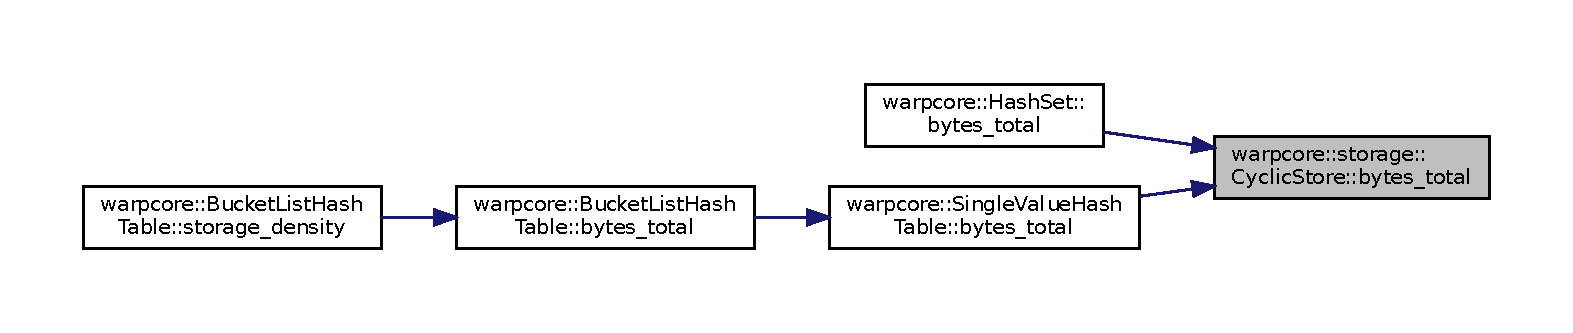
\includegraphics[width=350pt]{classwarpcore_1_1storage_1_1CyclicStore_ae65e099d0cfe170fc4cd2f02682c3bda_icgraph}
\end{center}
\end{figure}
\mbox{\Hypertarget{classwarpcore_1_1storage_1_1CyclicStore_acc4bfbb9b10868a193301d0ec5a46711}\label{classwarpcore_1_1storage_1_1CyclicStore_acc4bfbb9b10868a193301d0ec5a46711}} 
\index{warpcore\+::storage\+::\+Cyclic\+Store@{warpcore\+::storage\+::\+Cyclic\+Store}!capacity@{capacity}}
\index{capacity@{capacity}!warpcore\+::storage\+::\+Cyclic\+Store@{warpcore\+::storage\+::\+Cyclic\+Store}}
\subsubsection{\texorpdfstring{capacity()}{capacity()}}
{\footnotesize\ttfamily template$<$class T$>$ \\
\+\_\+\+\_\+host\+\_\+\+\_\+ index\+\_\+type \hyperlink{classwarpcore_1_1storage_1_1CyclicStore}{warpcore\+::storage\+::\+Cyclic\+Store}$<$ T $>$\+::capacity (\begin{DoxyParamCaption}{ }\end{DoxyParamCaption}) const\hspace{0.3cm}{\ttfamily [inline]}, {\ttfamily [noexcept]}}



get buffer capacity 

\begin{DoxyReturn}{Returns}
capacity 
\end{DoxyReturn}
Here is the caller graph for this function\+:
\nopagebreak
\begin{figure}[H]
\begin{center}
\leavevmode
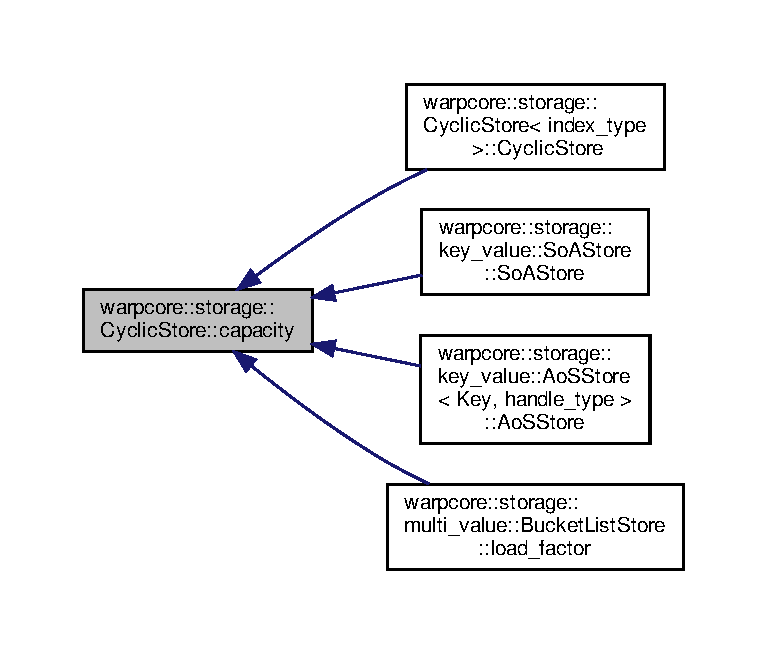
\includegraphics[width=350pt]{classwarpcore_1_1storage_1_1CyclicStore_acc4bfbb9b10868a193301d0ec5a46711_icgraph}
\end{center}
\end{figure}
\mbox{\Hypertarget{classwarpcore_1_1storage_1_1CyclicStore_ab475e047f32b8a8358ea6b78dfe2536d}\label{classwarpcore_1_1storage_1_1CyclicStore_ab475e047f32b8a8358ea6b78dfe2536d}} 
\index{warpcore\+::storage\+::\+Cyclic\+Store@{warpcore\+::storage\+::\+Cyclic\+Store}!get@{get}}
\index{get@{get}!warpcore\+::storage\+::\+Cyclic\+Store@{warpcore\+::storage\+::\+Cyclic\+Store}}
\subsubsection{\texorpdfstring{get()}{get()}}
{\footnotesize\ttfamily template$<$class T$>$ \\
\+\_\+\+\_\+host\+\_\+\+\_\+ T$\ast$ \hyperlink{classwarpcore_1_1storage_1_1CyclicStore}{warpcore\+::storage\+::\+Cyclic\+Store}$<$ T $>$\+::get (\begin{DoxyParamCaption}{ }\end{DoxyParamCaption}) const\hspace{0.3cm}{\ttfamily [inline]}, {\ttfamily [noexcept]}}



atomically fetches the next slot in the buffer 

\begin{DoxyReturn}{Returns}
pointer to the next slot in the buffer  {\ttfamily const} on purpose 
\end{DoxyReturn}
Here is the caller graph for this function\+:
\nopagebreak
\begin{figure}[H]
\begin{center}
\leavevmode
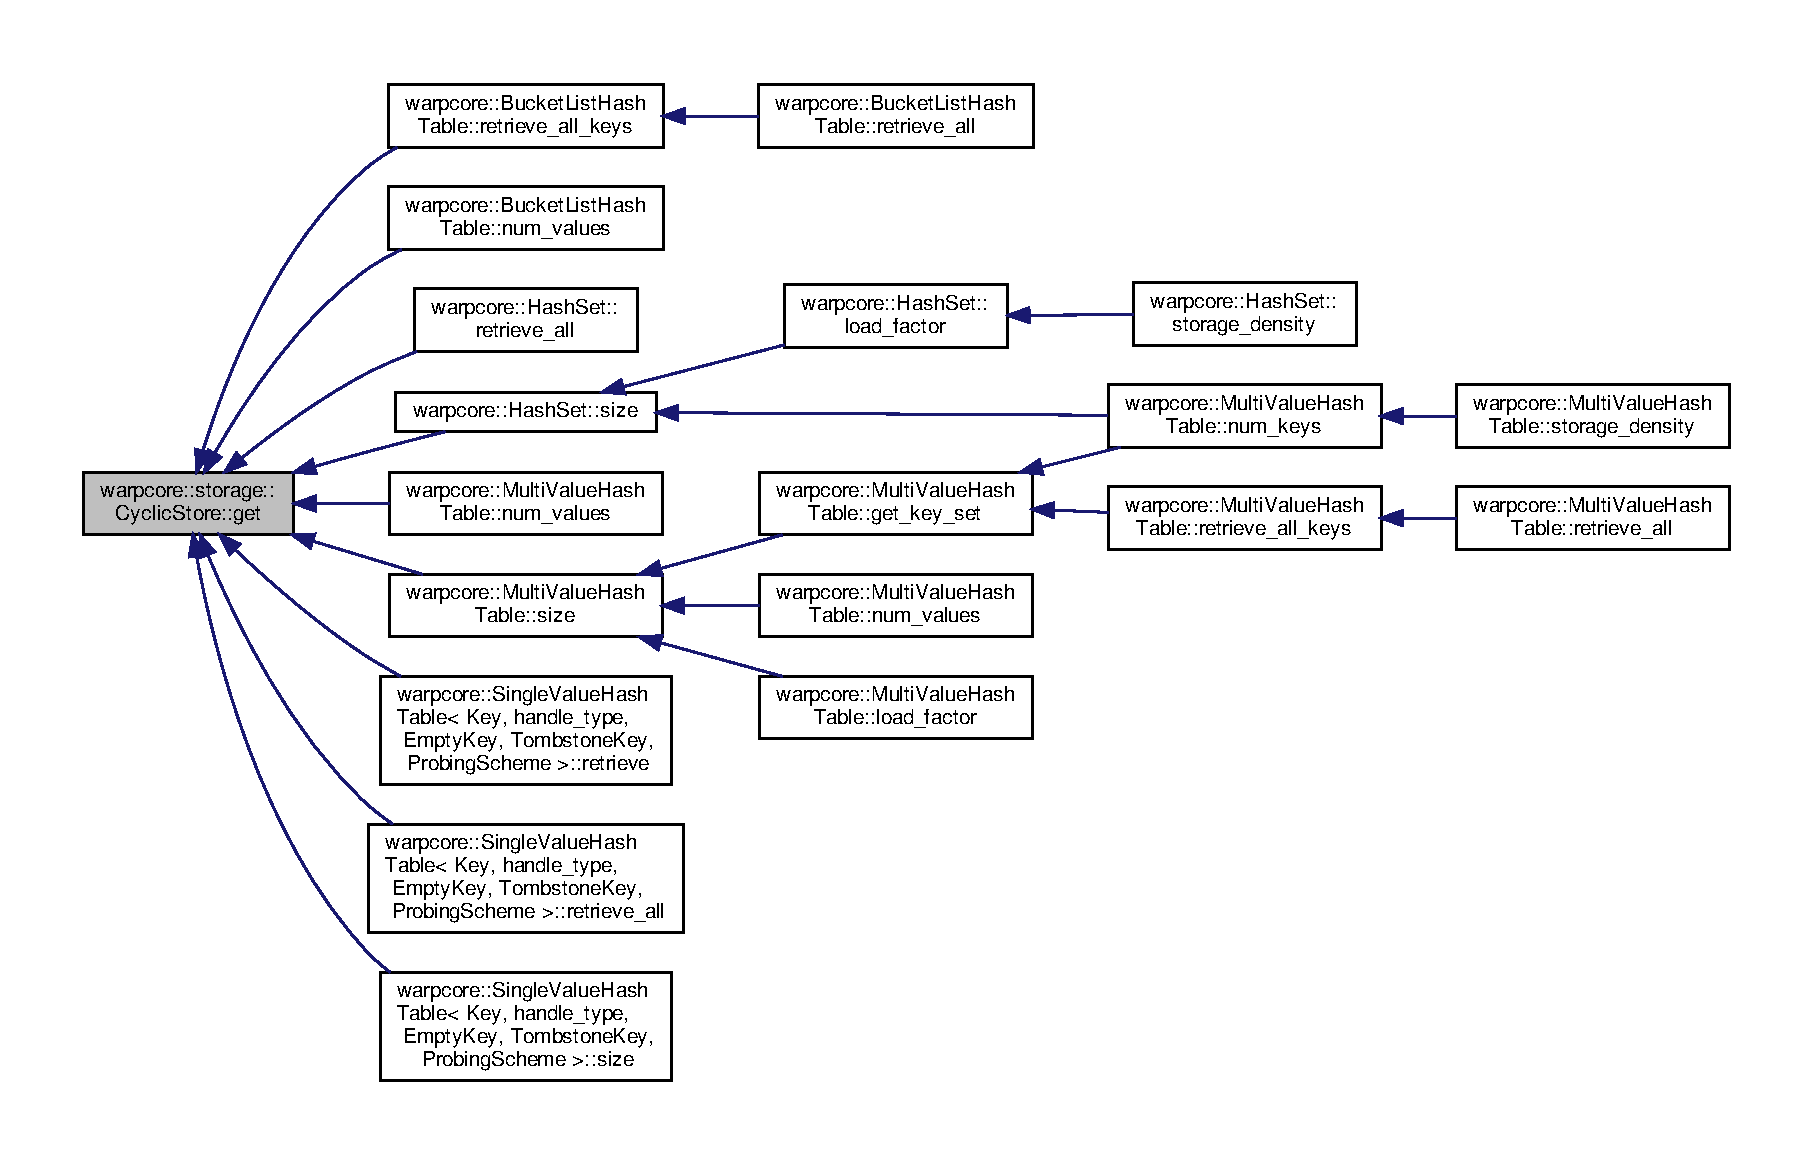
\includegraphics[width=350pt]{classwarpcore_1_1storage_1_1CyclicStore_ab475e047f32b8a8358ea6b78dfe2536d_icgraph}
\end{center}
\end{figure}
\mbox{\Hypertarget{classwarpcore_1_1storage_1_1CyclicStore_ab6c224b2b5a49d93dc7e052ec7b8cc32}\label{classwarpcore_1_1storage_1_1CyclicStore_ab6c224b2b5a49d93dc7e052ec7b8cc32}} 
\index{warpcore\+::storage\+::\+Cyclic\+Store@{warpcore\+::storage\+::\+Cyclic\+Store}!status@{status}}
\index{status@{status}!warpcore\+::storage\+::\+Cyclic\+Store@{warpcore\+::storage\+::\+Cyclic\+Store}}
\subsubsection{\texorpdfstring{status()}{status()}}
{\footnotesize\ttfamily template$<$class T$>$ \\
\+\_\+\+\_\+host\+\_\+\+\_\+ \hyperlink{classwarpcore_1_1Status}{status\+\_\+type} \hyperlink{classwarpcore_1_1storage_1_1CyclicStore}{warpcore\+::storage\+::\+Cyclic\+Store}$<$ T $>$\+::status (\begin{DoxyParamCaption}{ }\end{DoxyParamCaption}) const\hspace{0.3cm}{\ttfamily [inline]}, {\ttfamily [noexcept]}}



get buffer status 

\begin{DoxyReturn}{Returns}
status 
\end{DoxyReturn}
Here is the caller graph for this function\+:
\nopagebreak
\begin{figure}[H]
\begin{center}
\leavevmode
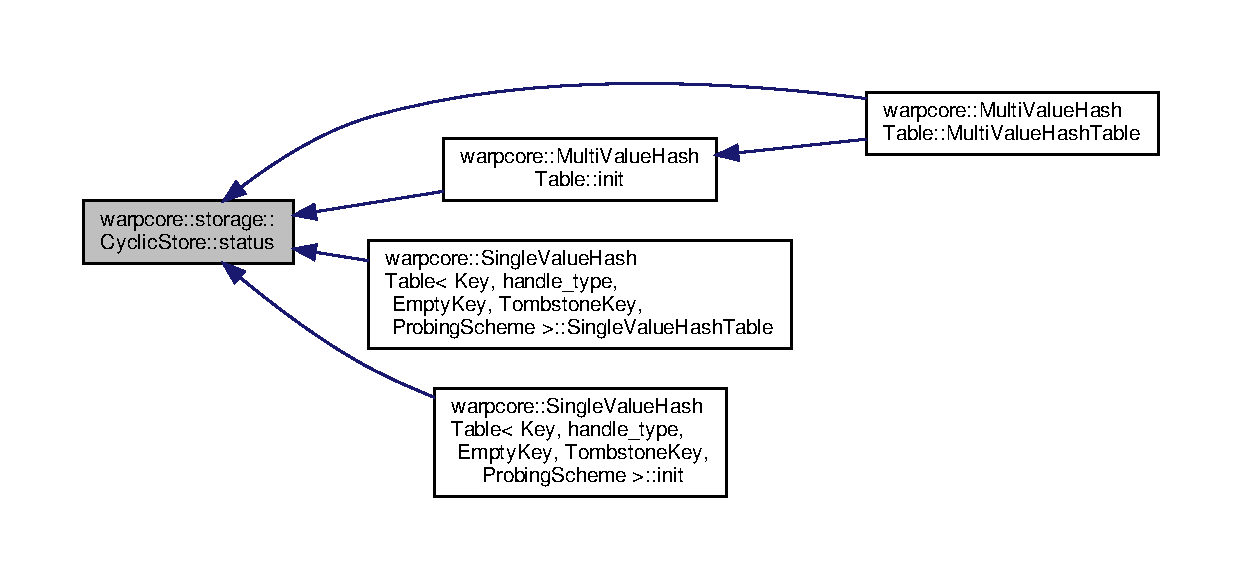
\includegraphics[width=350pt]{classwarpcore_1_1storage_1_1CyclicStore_ab6c224b2b5a49d93dc7e052ec7b8cc32_icgraph}
\end{center}
\end{figure}

\hypertarget{classwarpcore_1_1probing__schemes_1_1DoubleHashing}{}\section{warpcore\+:\+:probing\+\_\+schemes\+:\+:Double\+Hashing$<$ Hasher1, Hasher2, C\+G\+Size $>$ Class Template Reference}
\label{classwarpcore_1_1probing__schemes_1_1DoubleHashing}\index{warpcore\+::probing\+\_\+schemes\+::\+Double\+Hashing$<$ Hasher1, Hasher2, C\+G\+Size $>$@{warpcore\+::probing\+\_\+schemes\+::\+Double\+Hashing$<$ Hasher1, Hasher2, C\+G\+Size $>$}}


double hashing scheme\+: $hash(k,i) = h_1(k)+i\cdot h_2(k)$  


\subsection*{Public Types}
\begin{DoxyCompactItemize}
\item 
\mbox{\Hypertarget{classwarpcore_1_1probing__schemes_1_1DoubleHashing_a7717ccd60167090680b7049a3ea59645}\label{classwarpcore_1_1probing__schemes_1_1DoubleHashing_a7717ccd60167090680b7049a3ea59645}} 
using {\bfseries key\+\_\+type} = typename Hasher1\+::key\+\_\+type
\item 
\mbox{\Hypertarget{classwarpcore_1_1probing__schemes_1_1DoubleHashing_a806df26c5d213788a298771b746788a5}\label{classwarpcore_1_1probing__schemes_1_1DoubleHashing_a806df26c5d213788a298771b746788a5}} 
using {\bfseries index\+\_\+type} = index\+\_\+t
\item 
\mbox{\Hypertarget{classwarpcore_1_1probing__schemes_1_1DoubleHashing_a3fb4fb42e3e21599e2a1909cd0df5e37}\label{classwarpcore_1_1probing__schemes_1_1DoubleHashing_a3fb4fb42e3e21599e2a1909cd0df5e37}} 
using {\bfseries tag} = tags\+::probing\+\_\+scheme\+\_\+tag
\end{DoxyCompactItemize}
\subsection*{Public Member Functions}
\begin{DoxyCompactItemize}
\item 
\+\_\+\+\_\+device\+\_\+\+\_\+ \hyperlink{classwarpcore_1_1probing__schemes_1_1DoubleHashing_aa74ed01c96665a5651ad4dc1395da1d2}{Double\+Hashing} (index\+\_\+type capacity, index\+\_\+type probing\+\_\+length, const cg\+::thread\+\_\+block\+\_\+tile$<$ C\+G\+Size $>$ \&group)
\begin{DoxyCompactList}\small\item\em constructor \end{DoxyCompactList}\item 
\mbox{\Hypertarget{classwarpcore_1_1probing__schemes_1_1DoubleHashing_ab99320ff4f7ca5b001b38c657eee8f45}\label{classwarpcore_1_1probing__schemes_1_1DoubleHashing_ab99320ff4f7ca5b001b38c657eee8f45}} 
{\footnotesize template$<$class T $>$ }\\\+\_\+\+\_\+device\+\_\+\+\_\+ index\+\_\+type {\bfseries begin} (T, T)=delete
\item 
\mbox{\Hypertarget{classwarpcore_1_1probing__schemes_1_1DoubleHashing_aa7def8460dd3b81b53577401ef79dcaf}\label{classwarpcore_1_1probing__schemes_1_1DoubleHashing_aa7def8460dd3b81b53577401ef79dcaf}} 
{\footnotesize template$<$class T $>$ }\\\+\_\+\+\_\+device\+\_\+\+\_\+ index\+\_\+type {\bfseries begin} (T)=delete
\item 
\+\_\+\+\_\+device\+\_\+\+\_\+ index\+\_\+type \hyperlink{classwarpcore_1_1probing__schemes_1_1DoubleHashing_abd3749c428220cad1193fc9b2994d545}{begin} (key\+\_\+type key, key\+\_\+type seed=0) noexcept
\begin{DoxyCompactList}\small\item\em begin probing sequence \end{DoxyCompactList}\item 
\+\_\+\+\_\+device\+\_\+\+\_\+ index\+\_\+type \hyperlink{classwarpcore_1_1probing__schemes_1_1DoubleHashing_a49bf8de6c8af2e84d335e62a864a1a75}{next} () noexcept
\begin{DoxyCompactList}\small\item\em next probing index for {\ttfamily key} \end{DoxyCompactList}\end{DoxyCompactItemize}
\subsection*{Static Public Member Functions}
\begin{DoxyCompactItemize}
\item 
static \+\_\+\+\_\+host\+\_\+\+\_\+\+\_\+\+\_\+device\+\_\+\+\_\+ constexpr index\+\_\+type \hyperlink{classwarpcore_1_1probing__schemes_1_1DoubleHashing_ae94c09166e06d7d1d147959ca174e1b1}{cg\+\_\+size} () noexcept
\begin{DoxyCompactList}\small\item\em get cooperative group size \end{DoxyCompactList}\item 
static \+\_\+\+\_\+device\+\_\+\+\_\+ constexpr index\+\_\+type \hyperlink{classwarpcore_1_1probing__schemes_1_1DoubleHashing_ac9ee12c8aa2a976f3fd2cdee3bac4957}{end} () noexcept
\begin{DoxyCompactList}\small\item\em end specifier of probing sequence \end{DoxyCompactList}\end{DoxyCompactItemize}


\subsection{Detailed Description}
\subsubsection*{template$<$class Hasher1, class Hasher2, index\+\_\+t C\+G\+Size = 1$>$\newline
class warpcore\+::probing\+\_\+schemes\+::\+Double\+Hashing$<$ Hasher1, Hasher2, C\+G\+Size $>$}

double hashing scheme\+: $hash(k,i) = h_1(k)+i\cdot h_2(k)$ 


\begin{DoxyTemplParams}{Template Parameters}
{\em Hasher1} & first hash function \\
\hline
{\em Hasher1} & second hash function \\
\hline
{\em C\+G\+Size} & cooperative group size \\
\hline
\end{DoxyTemplParams}


\subsection{Constructor \& Destructor Documentation}
\mbox{\Hypertarget{classwarpcore_1_1probing__schemes_1_1DoubleHashing_aa74ed01c96665a5651ad4dc1395da1d2}\label{classwarpcore_1_1probing__schemes_1_1DoubleHashing_aa74ed01c96665a5651ad4dc1395da1d2}} 
\index{warpcore\+::probing\+\_\+schemes\+::\+Double\+Hashing@{warpcore\+::probing\+\_\+schemes\+::\+Double\+Hashing}!Double\+Hashing@{Double\+Hashing}}
\index{Double\+Hashing@{Double\+Hashing}!warpcore\+::probing\+\_\+schemes\+::\+Double\+Hashing@{warpcore\+::probing\+\_\+schemes\+::\+Double\+Hashing}}
\subsubsection{\texorpdfstring{Double\+Hashing()}{DoubleHashing()}}
{\footnotesize\ttfamily template$<$class Hasher1 , class Hasher2 , index\+\_\+t C\+G\+Size = 1$>$ \\
\+\_\+\+\_\+device\+\_\+\+\_\+ \hyperlink{classwarpcore_1_1probing__schemes_1_1DoubleHashing}{warpcore\+::probing\+\_\+schemes\+::\+Double\+Hashing}$<$ Hasher1, Hasher2, C\+G\+Size $>$\+::\hyperlink{classwarpcore_1_1probing__schemes_1_1DoubleHashing}{Double\+Hashing} (\begin{DoxyParamCaption}\item[{index\+\_\+type}]{capacity,  }\item[{index\+\_\+type}]{probing\+\_\+length,  }\item[{const cg\+::thread\+\_\+block\+\_\+tile$<$ C\+G\+Size $>$ \&}]{group }\end{DoxyParamCaption})\hspace{0.3cm}{\ttfamily [inline]}, {\ttfamily [explicit]}}



constructor 


\begin{DoxyParams}[1]{Parameters}
\mbox{\tt in}  & {\em capacity} & capacity of the underlying hash table \\
\hline
\mbox{\tt in}  & {\em probing\+\_\+length} & number of probing attempts \\
\hline
\mbox{\tt in}  & {\em group} & cooperative group \\
\hline
\end{DoxyParams}


\subsection{Member Function Documentation}
\mbox{\Hypertarget{classwarpcore_1_1probing__schemes_1_1DoubleHashing_abd3749c428220cad1193fc9b2994d545}\label{classwarpcore_1_1probing__schemes_1_1DoubleHashing_abd3749c428220cad1193fc9b2994d545}} 
\index{warpcore\+::probing\+\_\+schemes\+::\+Double\+Hashing@{warpcore\+::probing\+\_\+schemes\+::\+Double\+Hashing}!begin@{begin}}
\index{begin@{begin}!warpcore\+::probing\+\_\+schemes\+::\+Double\+Hashing@{warpcore\+::probing\+\_\+schemes\+::\+Double\+Hashing}}
\subsubsection{\texorpdfstring{begin()}{begin()}}
{\footnotesize\ttfamily template$<$class Hasher1 , class Hasher2 , index\+\_\+t C\+G\+Size = 1$>$ \\
\+\_\+\+\_\+device\+\_\+\+\_\+ index\+\_\+type \hyperlink{classwarpcore_1_1probing__schemes_1_1DoubleHashing}{warpcore\+::probing\+\_\+schemes\+::\+Double\+Hashing}$<$ Hasher1, Hasher2, C\+G\+Size $>$\+::begin (\begin{DoxyParamCaption}\item[{key\+\_\+type}]{key,  }\item[{key\+\_\+type}]{seed = {\ttfamily 0} }\end{DoxyParamCaption})\hspace{0.3cm}{\ttfamily [inline]}, {\ttfamily [noexcept]}}



begin probing sequence 


\begin{DoxyParams}[1]{Parameters}
\mbox{\tt in}  & {\em key} & key to be probed \\
\hline
\mbox{\tt in}  & {\em seed} & random seed \\
\hline
\end{DoxyParams}
\begin{DoxyReturn}{Returns}
initial probing index for {\ttfamily key} 
\end{DoxyReturn}
\mbox{\Hypertarget{classwarpcore_1_1probing__schemes_1_1DoubleHashing_ae94c09166e06d7d1d147959ca174e1b1}\label{classwarpcore_1_1probing__schemes_1_1DoubleHashing_ae94c09166e06d7d1d147959ca174e1b1}} 
\index{warpcore\+::probing\+\_\+schemes\+::\+Double\+Hashing@{warpcore\+::probing\+\_\+schemes\+::\+Double\+Hashing}!cg\+\_\+size@{cg\+\_\+size}}
\index{cg\+\_\+size@{cg\+\_\+size}!warpcore\+::probing\+\_\+schemes\+::\+Double\+Hashing@{warpcore\+::probing\+\_\+schemes\+::\+Double\+Hashing}}
\subsubsection{\texorpdfstring{cg\+\_\+size()}{cg\_size()}}
{\footnotesize\ttfamily template$<$class Hasher1 , class Hasher2 , index\+\_\+t C\+G\+Size = 1$>$ \\
static \+\_\+\+\_\+host\+\_\+\+\_\+\+\_\+\+\_\+device\+\_\+\+\_\+ constexpr index\+\_\+type \hyperlink{classwarpcore_1_1probing__schemes_1_1DoubleHashing}{warpcore\+::probing\+\_\+schemes\+::\+Double\+Hashing}$<$ Hasher1, Hasher2, C\+G\+Size $>$\+::cg\+\_\+size (\begin{DoxyParamCaption}{ }\end{DoxyParamCaption})\hspace{0.3cm}{\ttfamily [inline]}, {\ttfamily [static]}, {\ttfamily [noexcept]}}



get cooperative group size 

\begin{DoxyReturn}{Returns}
cooperative group size 
\end{DoxyReturn}
\mbox{\Hypertarget{classwarpcore_1_1probing__schemes_1_1DoubleHashing_ac9ee12c8aa2a976f3fd2cdee3bac4957}\label{classwarpcore_1_1probing__schemes_1_1DoubleHashing_ac9ee12c8aa2a976f3fd2cdee3bac4957}} 
\index{warpcore\+::probing\+\_\+schemes\+::\+Double\+Hashing@{warpcore\+::probing\+\_\+schemes\+::\+Double\+Hashing}!end@{end}}
\index{end@{end}!warpcore\+::probing\+\_\+schemes\+::\+Double\+Hashing@{warpcore\+::probing\+\_\+schemes\+::\+Double\+Hashing}}
\subsubsection{\texorpdfstring{end()}{end()}}
{\footnotesize\ttfamily template$<$class Hasher1 , class Hasher2 , index\+\_\+t C\+G\+Size = 1$>$ \\
static \+\_\+\+\_\+device\+\_\+\+\_\+ constexpr index\+\_\+type \hyperlink{classwarpcore_1_1probing__schemes_1_1DoubleHashing}{warpcore\+::probing\+\_\+schemes\+::\+Double\+Hashing}$<$ Hasher1, Hasher2, C\+G\+Size $>$\+::end (\begin{DoxyParamCaption}{ }\end{DoxyParamCaption})\hspace{0.3cm}{\ttfamily [inline]}, {\ttfamily [static]}, {\ttfamily [noexcept]}}



end specifier of probing sequence 

\begin{DoxyReturn}{Returns}
end specifier 
\end{DoxyReturn}
Here is the caller graph for this function\+:
\nopagebreak
\begin{figure}[H]
\begin{center}
\leavevmode
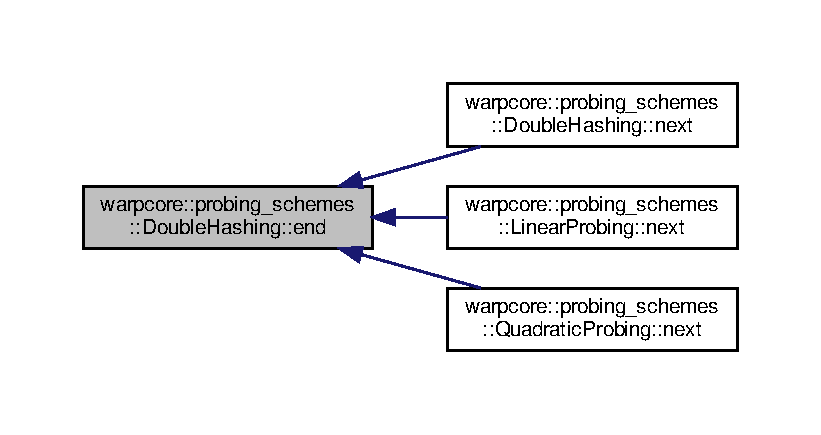
\includegraphics[width=350pt]{classwarpcore_1_1probing__schemes_1_1DoubleHashing_ac9ee12c8aa2a976f3fd2cdee3bac4957_icgraph}
\end{center}
\end{figure}
\mbox{\Hypertarget{classwarpcore_1_1probing__schemes_1_1DoubleHashing_a49bf8de6c8af2e84d335e62a864a1a75}\label{classwarpcore_1_1probing__schemes_1_1DoubleHashing_a49bf8de6c8af2e84d335e62a864a1a75}} 
\index{warpcore\+::probing\+\_\+schemes\+::\+Double\+Hashing@{warpcore\+::probing\+\_\+schemes\+::\+Double\+Hashing}!next@{next}}
\index{next@{next}!warpcore\+::probing\+\_\+schemes\+::\+Double\+Hashing@{warpcore\+::probing\+\_\+schemes\+::\+Double\+Hashing}}
\subsubsection{\texorpdfstring{next()}{next()}}
{\footnotesize\ttfamily template$<$class Hasher1 , class Hasher2 , index\+\_\+t C\+G\+Size = 1$>$ \\
\+\_\+\+\_\+device\+\_\+\+\_\+ index\+\_\+type \hyperlink{classwarpcore_1_1probing__schemes_1_1DoubleHashing}{warpcore\+::probing\+\_\+schemes\+::\+Double\+Hashing}$<$ Hasher1, Hasher2, C\+G\+Size $>$\+::next (\begin{DoxyParamCaption}{ }\end{DoxyParamCaption})\hspace{0.3cm}{\ttfamily [inline]}, {\ttfamily [noexcept]}}



next probing index for {\ttfamily key} 

\begin{DoxyReturn}{Returns}
next probing index for {\ttfamily key} 
\end{DoxyReturn}
Here is the call graph for this function\+:
\nopagebreak
\begin{figure}[H]
\begin{center}
\leavevmode
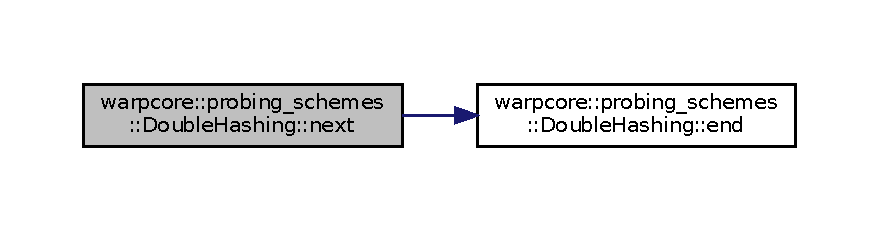
\includegraphics[width=350pt]{classwarpcore_1_1probing__schemes_1_1DoubleHashing_a49bf8de6c8af2e84d335e62a864a1a75_cgraph}
\end{center}
\end{figure}

\hypertarget{classwarpcore_1_1storage_1_1multi__value_1_1DynamicSlabListStore}{}\section{warpcore\+:\+:storage\+:\+:multi\+\_\+value\+:\+:Dynamic\+Slab\+List\+Store$<$ Value, Slab\+Index\+Bits, Value\+Counter\+Bits, Slab\+Size\+Bits $>$ Class Template Reference}
\label{classwarpcore_1_1storage_1_1multi__value_1_1DynamicSlabListStore}\index{warpcore\+::storage\+::multi\+\_\+value\+::\+Dynamic\+Slab\+List\+Store$<$ Value, Slab\+Index\+Bits, Value\+Counter\+Bits, Slab\+Size\+Bits $>$@{warpcore\+::storage\+::multi\+\_\+value\+::\+Dynamic\+Slab\+List\+Store$<$ Value, Slab\+Index\+Bits, Value\+Counter\+Bits, Slab\+Size\+Bits $>$}}


value store consisting of growing linked slabs of values  


\subsection*{Public Types}
\begin{DoxyCompactItemize}
\item 
\mbox{\Hypertarget{classwarpcore_1_1storage_1_1multi__value_1_1DynamicSlabListStore_aef0ce2b1fce731fb35a82f9eb2b0a84b}\label{classwarpcore_1_1storage_1_1multi__value_1_1DynamicSlabListStore_aef0ce2b1fce731fb35a82f9eb2b0a84b}} 
using {\bfseries value\+\_\+type} = Value
\item 
\mbox{\Hypertarget{classwarpcore_1_1storage_1_1multi__value_1_1DynamicSlabListStore_a5d04964b4d54427e763c76eabefb4e92}\label{classwarpcore_1_1storage_1_1multi__value_1_1DynamicSlabListStore_a5d04964b4d54427e763c76eabefb4e92}} 
using {\bfseries handle\+\_\+type} = detail\+::\+Dynamic\+Slab\+List\+Handle$<$ \hyperlink{classwarpcore_1_1storage_1_1multi__value_1_1DynamicSlabListStore}{type} $>$
\item 
\mbox{\Hypertarget{classwarpcore_1_1storage_1_1multi__value_1_1DynamicSlabListStore_aecd66efa9d87c97ecca83d1c09c2deff}\label{classwarpcore_1_1storage_1_1multi__value_1_1DynamicSlabListStore_aecd66efa9d87c97ecca83d1c09c2deff}} 
using {\bfseries index\+\_\+type} = index\+\_\+t
\item 
\mbox{\Hypertarget{classwarpcore_1_1storage_1_1multi__value_1_1DynamicSlabListStore_a7da4283d7b7d754d56cb37b7ba13a33e}\label{classwarpcore_1_1storage_1_1multi__value_1_1DynamicSlabListStore_a7da4283d7b7d754d56cb37b7ba13a33e}} 
using {\bfseries status\+\_\+type} = \hyperlink{classwarpcore_1_1Status}{Status}
\item 
\mbox{\Hypertarget{classwarpcore_1_1storage_1_1multi__value_1_1DynamicSlabListStore_a1a35ca0d04bcbeb0dc40b0a26bace242}\label{classwarpcore_1_1storage_1_1multi__value_1_1DynamicSlabListStore_a1a35ca0d04bcbeb0dc40b0a26bace242}} 
using {\bfseries slab\+\_\+type} = detail\+::\+Dynamic\+Slab$<$ \hyperlink{classwarpcore_1_1storage_1_1multi__value_1_1DynamicSlabListStore}{type} $>$
\item 
\mbox{\Hypertarget{classwarpcore_1_1storage_1_1multi__value_1_1DynamicSlabListStore_a8699cd13072e14dc60eac3c0d0ec96e2}\label{classwarpcore_1_1storage_1_1multi__value_1_1DynamicSlabListStore_a8699cd13072e14dc60eac3c0d0ec96e2}} 
using {\bfseries tag} = tags\+::dynamic\+\_\+value\+\_\+storage\+\_\+tag
\end{DoxyCompactItemize}
\subsection*{Public Member Functions}
\begin{DoxyCompactItemize}
\item 
\+\_\+\+\_\+host\+\_\+\+\_\+ \hyperlink{classwarpcore_1_1storage_1_1multi__value_1_1DynamicSlabListStore_ab0c3eb9a8eaef07da0eb5d7d3c5f026a}{Dynamic\+Slab\+List\+Store} (index\+\_\+type max\+\_\+capacity, float \hyperlink{classwarpcore_1_1storage_1_1multi__value_1_1DynamicSlabListStore_a79fb2a41f22cf59f4edf49c3de82d9dd}{slab\+\_\+grow\+\_\+factor}=2.\+0, index\+\_\+type \hyperlink{classwarpcore_1_1storage_1_1multi__value_1_1DynamicSlabListStore_adb7da0e5836a0274de92f906acaf7a43}{min\+\_\+slab\+\_\+size}=1, index\+\_\+type \hyperlink{classwarpcore_1_1storage_1_1multi__value_1_1DynamicSlabListStore_a58f11e19acf684db903b7985364ec73c}{max\+\_\+slab\+\_\+size}=handle\+\_\+type\+::max\+\_\+slab\+\_\+size()) noexcept
\begin{DoxyCompactList}\small\item\em constructor \end{DoxyCompactList}\item 
\+\_\+\+\_\+host\+\_\+\+\_\+\+\_\+\+\_\+device\+\_\+\+\_\+ \hyperlink{classwarpcore_1_1storage_1_1multi__value_1_1DynamicSlabListStore_a93d49c0a887055b282000cba031688d5}{Dynamic\+Slab\+List\+Store} (const \hyperlink{classwarpcore_1_1storage_1_1multi__value_1_1DynamicSlabListStore}{Dynamic\+Slab\+List\+Store} \&o) noexcept
\begin{DoxyCompactList}\small\item\em copy-\/constructor (shallow) \end{DoxyCompactList}\item 
\+\_\+\+\_\+host\+\_\+\+\_\+ \hyperlink{classwarpcore_1_1storage_1_1multi__value_1_1DynamicSlabListStore_a7be0cfee3a16cba0eb6296168d518a58}{Dynamic\+Slab\+List\+Store} (\hyperlink{classwarpcore_1_1storage_1_1multi__value_1_1DynamicSlabListStore}{Dynamic\+Slab\+List\+Store} \&\&o) noexcept
\begin{DoxyCompactList}\small\item\em move-\/constructor \end{DoxyCompactList}\item 
\mbox{\Hypertarget{classwarpcore_1_1storage_1_1multi__value_1_1DynamicSlabListStore_ab53d32d2ef4976130ae986c866802b6d}\label{classwarpcore_1_1storage_1_1multi__value_1_1DynamicSlabListStore_ab53d32d2ef4976130ae986c866802b6d}} 
\+\_\+\+\_\+host\+\_\+\+\_\+ \hyperlink{classwarpcore_1_1storage_1_1multi__value_1_1DynamicSlabListStore_ab53d32d2ef4976130ae986c866802b6d}{$\sim$\+Dynamic\+Slab\+List\+Store} () noexcept
\begin{DoxyCompactList}\small\item\em destructor \end{DoxyCompactList}\item 
\+\_\+\+\_\+host\+\_\+\+\_\+ void \hyperlink{classwarpcore_1_1storage_1_1multi__value_1_1DynamicSlabListStore_aa04bc2372b17856c61acd08d07381315}{init} (cuda\+Stream\+\_\+t stream=0) noexcept
\begin{DoxyCompactList}\small\item\em (re)initialize storage \end{DoxyCompactList}\item 
\+\_\+\+\_\+device\+\_\+\+\_\+ \hyperlink{classwarpcore_1_1Status}{status\+\_\+type} \hyperlink{classwarpcore_1_1storage_1_1multi__value_1_1DynamicSlabListStore_adc50985c5bd1ed3b507c1e3c7dda16db}{append} (handle\+\_\+type \&handle, const value\+\_\+type \&value) noexcept
\begin{DoxyCompactList}\small\item\em append a value to a slab list \end{DoxyCompactList}\item 
{\footnotesize template$<$class Func $>$ }\\\+\_\+\+\_\+device\+\_\+\+\_\+ void \hyperlink{classwarpcore_1_1storage_1_1multi__value_1_1DynamicSlabListStore_a58a0c59ab8d635869043921c9ec85c21}{for\+\_\+each} (handle\+\_\+type handle, Func f, const cg\+::thread\+\_\+group \&group=cg\+::this\+\_\+thread()) const noexcept
\begin{DoxyCompactList}\small\item\em apply a (lambda-\/)function on each value inside a slab list \end{DoxyCompactList}\item 
\+\_\+\+\_\+host\+\_\+\+\_\+\+\_\+\+\_\+device\+\_\+\+\_\+ \hyperlink{classwarpcore_1_1Status}{status\+\_\+type} \hyperlink{classwarpcore_1_1storage_1_1multi__value_1_1DynamicSlabListStore_a9f67ef2bd0b072938bce462656b2c8aa}{status} () const noexcept
\begin{DoxyCompactList}\small\item\em get status \end{DoxyCompactList}\item 
\+\_\+\+\_\+host\+\_\+\+\_\+\+\_\+\+\_\+device\+\_\+\+\_\+ index\+\_\+type \hyperlink{classwarpcore_1_1storage_1_1multi__value_1_1DynamicSlabListStore_ae1c489e608b429bb34ad138c59aded93}{capacity} () const noexcept
\begin{DoxyCompactList}\small\item\em get maximum value capacity \end{DoxyCompactList}\item 
\+\_\+\+\_\+host\+\_\+\+\_\+\+\_\+\+\_\+device\+\_\+\+\_\+ float \hyperlink{classwarpcore_1_1storage_1_1multi__value_1_1DynamicSlabListStore_ab9e38febbac249da5662580311a76f06}{load\+\_\+factor} (cuda\+Stream\+\_\+t stream=0) const noexcept
\begin{DoxyCompactList}\small\item\em get load factor \end{DoxyCompactList}\item 
\+\_\+\+\_\+host\+\_\+\+\_\+\+\_\+\+\_\+device\+\_\+\+\_\+ index\+\_\+type \hyperlink{classwarpcore_1_1storage_1_1multi__value_1_1DynamicSlabListStore_a98fbded6fb4603336d5ea64b6e01aec9}{bytes\+\_\+occupied} (cuda\+Stream\+\_\+t stream=0) const noexcept
\begin{DoxyCompactList}\small\item\em get the number of occupied bytes \end{DoxyCompactList}\item 
\+\_\+\+\_\+host\+\_\+\+\_\+\+\_\+\+\_\+device\+\_\+\+\_\+ float \hyperlink{classwarpcore_1_1storage_1_1multi__value_1_1DynamicSlabListStore_a79fb2a41f22cf59f4edf49c3de82d9dd}{slab\+\_\+grow\+\_\+factor} () const noexcept
\begin{DoxyCompactList}\small\item\em get slab growth factor \end{DoxyCompactList}\item 
\+\_\+\+\_\+host\+\_\+\+\_\+\+\_\+\+\_\+device\+\_\+\+\_\+ index\+\_\+type \hyperlink{classwarpcore_1_1storage_1_1multi__value_1_1DynamicSlabListStore_adb7da0e5836a0274de92f906acaf7a43}{min\+\_\+slab\+\_\+size} () const noexcept
\begin{DoxyCompactList}\small\item\em get minimum slab capacity \end{DoxyCompactList}\item 
\+\_\+\+\_\+host\+\_\+\+\_\+\+\_\+\+\_\+device\+\_\+\+\_\+ index\+\_\+type \hyperlink{classwarpcore_1_1storage_1_1multi__value_1_1DynamicSlabListStore_a58f11e19acf684db903b7985364ec73c}{max\+\_\+slab\+\_\+size} () const noexcept
\begin{DoxyCompactList}\small\item\em get maximum slab capacity \end{DoxyCompactList}\item 
\+\_\+\+\_\+host\+\_\+\+\_\+\+\_\+\+\_\+device\+\_\+\+\_\+ bool \hyperlink{classwarpcore_1_1storage_1_1multi__value_1_1DynamicSlabListStore_ac26c2496f6c97b1f9ecbd64baa3b8496}{is\+\_\+copy} () const noexcept
\begin{DoxyCompactList}\small\item\em indicates if this object is a shallow copy \end{DoxyCompactList}\end{DoxyCompactItemize}
\subsection*{Static Public Member Functions}
\begin{DoxyCompactItemize}
\item 
static \+\_\+\+\_\+host\+\_\+\+\_\+\+\_\+\+\_\+device\+\_\+\+\_\+ constexpr index\+\_\+type \hyperlink{classwarpcore_1_1storage_1_1multi__value_1_1DynamicSlabListStore_a20efaad0116184429778d736723c30f3}{slab\+\_\+index\+\_\+bits} () noexcept
\begin{DoxyCompactList}\small\item\em get number of bits used to enumerate slabs \end{DoxyCompactList}\item 
static \+\_\+\+\_\+host\+\_\+\+\_\+\+\_\+\+\_\+device\+\_\+\+\_\+ constexpr index\+\_\+type \hyperlink{classwarpcore_1_1storage_1_1multi__value_1_1DynamicSlabListStore_aff75cc3f371c2b31b569ff585f9ac900}{value\+\_\+counter\+\_\+bits} () noexcept
\begin{DoxyCompactList}\small\item\em get number of bits used to count values in a slab list \end{DoxyCompactList}\item 
static \+\_\+\+\_\+host\+\_\+\+\_\+\+\_\+\+\_\+device\+\_\+\+\_\+ constexpr index\+\_\+type \hyperlink{classwarpcore_1_1storage_1_1multi__value_1_1DynamicSlabListStore_a16f77ea7e30c30b17af19a229464ed42}{slab\+\_\+size\+\_\+bits} () noexcept
\begin{DoxyCompactList}\small\item\em get number of bits used to hold the value capacity of a slab \end{DoxyCompactList}\item 
static \+\_\+\+\_\+host\+\_\+\+\_\+\+\_\+\+\_\+device\+\_\+\+\_\+ constexpr handle\+\_\+type \hyperlink{classwarpcore_1_1storage_1_1multi__value_1_1DynamicSlabListStore_a647790aa072589d7296b7ea57436f297}{uninitialized\+\_\+handle} () noexcept
\begin{DoxyCompactList}\small\item\em get uninitialized handle \end{DoxyCompactList}\item 
static \+\_\+\+\_\+device\+\_\+\+\_\+ constexpr index\+\_\+type \hyperlink{classwarpcore_1_1storage_1_1multi__value_1_1DynamicSlabListStore_a79dffb54a0930061383f69bbc769c6d1}{size} (handle\+\_\+type handle) noexcept
\begin{DoxyCompactList}\small\item\em get number of values in slab list \end{DoxyCompactList}\end{DoxyCompactItemize}


\subsection{Detailed Description}
\subsubsection*{template$<$class Value, index\+\_\+t Slab\+Index\+Bits = 30, index\+\_\+t Value\+Counter\+Bits = 22, index\+\_\+t Slab\+Size\+Bits = 10$>$\newline
class warpcore\+::storage\+::multi\+\_\+value\+::\+Dynamic\+Slab\+List\+Store$<$ Value, Slab\+Index\+Bits, Value\+Counter\+Bits, Slab\+Size\+Bits $>$}

value store consisting of growing linked slabs of values 


\begin{DoxyTemplParams}{Template Parameters}
{\em Value} & type to store \\
\hline
{\em Slab\+Index\+Bits} & number of bits used to enumerate slab I\+Ds \\
\hline
{\em Value\+Counter\+Bits} & number of bits used to count values in a slab list \\
\hline
{\em Slab\+Size\+Bits} & number of bits used to hold the value capacity of a slab \\
\hline
\end{DoxyTemplParams}


\subsection{Constructor \& Destructor Documentation}
\mbox{\Hypertarget{classwarpcore_1_1storage_1_1multi__value_1_1DynamicSlabListStore_ab0c3eb9a8eaef07da0eb5d7d3c5f026a}\label{classwarpcore_1_1storage_1_1multi__value_1_1DynamicSlabListStore_ab0c3eb9a8eaef07da0eb5d7d3c5f026a}} 
\index{warpcore\+::storage\+::multi\+\_\+value\+::\+Dynamic\+Slab\+List\+Store@{warpcore\+::storage\+::multi\+\_\+value\+::\+Dynamic\+Slab\+List\+Store}!Dynamic\+Slab\+List\+Store@{Dynamic\+Slab\+List\+Store}}
\index{Dynamic\+Slab\+List\+Store@{Dynamic\+Slab\+List\+Store}!warpcore\+::storage\+::multi\+\_\+value\+::\+Dynamic\+Slab\+List\+Store@{warpcore\+::storage\+::multi\+\_\+value\+::\+Dynamic\+Slab\+List\+Store}}
\subsubsection{\texorpdfstring{Dynamic\+Slab\+List\+Store()}{DynamicSlabListStore()}\hspace{0.1cm}{\footnotesize\ttfamily [1/3]}}
{\footnotesize\ttfamily template$<$class Value , index\+\_\+t Slab\+Index\+Bits = 30, index\+\_\+t Value\+Counter\+Bits = 22, index\+\_\+t Slab\+Size\+Bits = 10$>$ \\
\+\_\+\+\_\+host\+\_\+\+\_\+ \hyperlink{classwarpcore_1_1storage_1_1multi__value_1_1DynamicSlabListStore}{warpcore\+::storage\+::multi\+\_\+value\+::\+Dynamic\+Slab\+List\+Store}$<$ Value, Slab\+Index\+Bits, Value\+Counter\+Bits, Slab\+Size\+Bits $>$\+::\hyperlink{classwarpcore_1_1storage_1_1multi__value_1_1DynamicSlabListStore}{Dynamic\+Slab\+List\+Store} (\begin{DoxyParamCaption}\item[{index\+\_\+type}]{max\+\_\+capacity,  }\item[{float}]{slab\+\_\+grow\+\_\+factor = {\ttfamily 2.0},  }\item[{index\+\_\+type}]{min\+\_\+slab\+\_\+size = {\ttfamily 1},  }\item[{index\+\_\+type}]{max\+\_\+slab\+\_\+size = {\ttfamily handle\+\_\+type\+:\+:max\+\_\+slab\+\_\+size()} }\end{DoxyParamCaption})\hspace{0.3cm}{\ttfamily [inline]}, {\ttfamily [explicit]}, {\ttfamily [noexcept]}}



constructor 


\begin{DoxyParams}[1]{Parameters}
\mbox{\tt in}  & {\em max\+\_\+capacity} & maximum number of value slots \\
\hline
\mbox{\tt in}  & {\em slab\+\_\+grow\+\_\+factor} & factor which determines the growth of each newly allocated slab \\
\hline
\mbox{\tt in}  & {\em min\+\_\+slab\+\_\+size} & value capacity of the first slab of a slab list \\
\hline
\mbox{\tt in}  & {\em max\+\_\+slab\+\_\+size} & value capacity after which no more growth is allowed for newly allocated slabs \\
\hline
\end{DoxyParams}
\mbox{\Hypertarget{classwarpcore_1_1storage_1_1multi__value_1_1DynamicSlabListStore_a93d49c0a887055b282000cba031688d5}\label{classwarpcore_1_1storage_1_1multi__value_1_1DynamicSlabListStore_a93d49c0a887055b282000cba031688d5}} 
\index{warpcore\+::storage\+::multi\+\_\+value\+::\+Dynamic\+Slab\+List\+Store@{warpcore\+::storage\+::multi\+\_\+value\+::\+Dynamic\+Slab\+List\+Store}!Dynamic\+Slab\+List\+Store@{Dynamic\+Slab\+List\+Store}}
\index{Dynamic\+Slab\+List\+Store@{Dynamic\+Slab\+List\+Store}!warpcore\+::storage\+::multi\+\_\+value\+::\+Dynamic\+Slab\+List\+Store@{warpcore\+::storage\+::multi\+\_\+value\+::\+Dynamic\+Slab\+List\+Store}}
\subsubsection{\texorpdfstring{Dynamic\+Slab\+List\+Store()}{DynamicSlabListStore()}\hspace{0.1cm}{\footnotesize\ttfamily [2/3]}}
{\footnotesize\ttfamily template$<$class Value , index\+\_\+t Slab\+Index\+Bits = 30, index\+\_\+t Value\+Counter\+Bits = 22, index\+\_\+t Slab\+Size\+Bits = 10$>$ \\
\+\_\+\+\_\+host\+\_\+\+\_\+\+\_\+\+\_\+device\+\_\+\+\_\+ \hyperlink{classwarpcore_1_1storage_1_1multi__value_1_1DynamicSlabListStore}{warpcore\+::storage\+::multi\+\_\+value\+::\+Dynamic\+Slab\+List\+Store}$<$ Value, Slab\+Index\+Bits, Value\+Counter\+Bits, Slab\+Size\+Bits $>$\+::\hyperlink{classwarpcore_1_1storage_1_1multi__value_1_1DynamicSlabListStore}{Dynamic\+Slab\+List\+Store} (\begin{DoxyParamCaption}\item[{const \hyperlink{classwarpcore_1_1storage_1_1multi__value_1_1DynamicSlabListStore}{Dynamic\+Slab\+List\+Store}$<$ Value, Slab\+Index\+Bits, Value\+Counter\+Bits, Slab\+Size\+Bits $>$ \&}]{o }\end{DoxyParamCaption})\hspace{0.3cm}{\ttfamily [inline]}, {\ttfamily [noexcept]}}



copy-\/constructor (shallow) 


\begin{DoxyParams}[1]{Parameters}
\mbox{\tt in}  & {\em object} & to be copied \\
\hline
\end{DoxyParams}
\mbox{\Hypertarget{classwarpcore_1_1storage_1_1multi__value_1_1DynamicSlabListStore_a7be0cfee3a16cba0eb6296168d518a58}\label{classwarpcore_1_1storage_1_1multi__value_1_1DynamicSlabListStore_a7be0cfee3a16cba0eb6296168d518a58}} 
\index{warpcore\+::storage\+::multi\+\_\+value\+::\+Dynamic\+Slab\+List\+Store@{warpcore\+::storage\+::multi\+\_\+value\+::\+Dynamic\+Slab\+List\+Store}!Dynamic\+Slab\+List\+Store@{Dynamic\+Slab\+List\+Store}}
\index{Dynamic\+Slab\+List\+Store@{Dynamic\+Slab\+List\+Store}!warpcore\+::storage\+::multi\+\_\+value\+::\+Dynamic\+Slab\+List\+Store@{warpcore\+::storage\+::multi\+\_\+value\+::\+Dynamic\+Slab\+List\+Store}}
\subsubsection{\texorpdfstring{Dynamic\+Slab\+List\+Store()}{DynamicSlabListStore()}\hspace{0.1cm}{\footnotesize\ttfamily [3/3]}}
{\footnotesize\ttfamily template$<$class Value , index\+\_\+t Slab\+Index\+Bits = 30, index\+\_\+t Value\+Counter\+Bits = 22, index\+\_\+t Slab\+Size\+Bits = 10$>$ \\
\+\_\+\+\_\+host\+\_\+\+\_\+ \hyperlink{classwarpcore_1_1storage_1_1multi__value_1_1DynamicSlabListStore}{warpcore\+::storage\+::multi\+\_\+value\+::\+Dynamic\+Slab\+List\+Store}$<$ Value, Slab\+Index\+Bits, Value\+Counter\+Bits, Slab\+Size\+Bits $>$\+::\hyperlink{classwarpcore_1_1storage_1_1multi__value_1_1DynamicSlabListStore}{Dynamic\+Slab\+List\+Store} (\begin{DoxyParamCaption}\item[{\hyperlink{classwarpcore_1_1storage_1_1multi__value_1_1DynamicSlabListStore}{Dynamic\+Slab\+List\+Store}$<$ Value, Slab\+Index\+Bits, Value\+Counter\+Bits, Slab\+Size\+Bits $>$ \&\&}]{o }\end{DoxyParamCaption})\hspace{0.3cm}{\ttfamily [inline]}, {\ttfamily [noexcept]}}



move-\/constructor 


\begin{DoxyParams}[1]{Parameters}
\mbox{\tt in}  & {\em object} & to be moved \\
\hline
\end{DoxyParams}


\subsection{Member Function Documentation}
\mbox{\Hypertarget{classwarpcore_1_1storage_1_1multi__value_1_1DynamicSlabListStore_adc50985c5bd1ed3b507c1e3c7dda16db}\label{classwarpcore_1_1storage_1_1multi__value_1_1DynamicSlabListStore_adc50985c5bd1ed3b507c1e3c7dda16db}} 
\index{warpcore\+::storage\+::multi\+\_\+value\+::\+Dynamic\+Slab\+List\+Store@{warpcore\+::storage\+::multi\+\_\+value\+::\+Dynamic\+Slab\+List\+Store}!append@{append}}
\index{append@{append}!warpcore\+::storage\+::multi\+\_\+value\+::\+Dynamic\+Slab\+List\+Store@{warpcore\+::storage\+::multi\+\_\+value\+::\+Dynamic\+Slab\+List\+Store}}
\subsubsection{\texorpdfstring{append()}{append()}}
{\footnotesize\ttfamily template$<$class Value , index\+\_\+t Slab\+Index\+Bits = 30, index\+\_\+t Value\+Counter\+Bits = 22, index\+\_\+t Slab\+Size\+Bits = 10$>$ \\
\+\_\+\+\_\+device\+\_\+\+\_\+ \hyperlink{classwarpcore_1_1Status}{status\+\_\+type} \hyperlink{classwarpcore_1_1storage_1_1multi__value_1_1DynamicSlabListStore}{warpcore\+::storage\+::multi\+\_\+value\+::\+Dynamic\+Slab\+List\+Store}$<$ Value, Slab\+Index\+Bits, Value\+Counter\+Bits, Slab\+Size\+Bits $>$\+::append (\begin{DoxyParamCaption}\item[{handle\+\_\+type \&}]{handle,  }\item[{const value\+\_\+type \&}]{value }\end{DoxyParamCaption})\hspace{0.3cm}{\ttfamily [inline]}, {\ttfamily [noexcept]}}



append a value to a slab list 


\begin{DoxyParams}[1]{Parameters}
\mbox{\tt in}  & {\em handle} & handle to the slab list \\
\hline
\mbox{\tt in}  & {\em value} & value to be inserted \\
\hline
\end{DoxyParams}
\begin{DoxyReturn}{Returns}
status 
\end{DoxyReturn}
\mbox{\Hypertarget{classwarpcore_1_1storage_1_1multi__value_1_1DynamicSlabListStore_a98fbded6fb4603336d5ea64b6e01aec9}\label{classwarpcore_1_1storage_1_1multi__value_1_1DynamicSlabListStore_a98fbded6fb4603336d5ea64b6e01aec9}} 
\index{warpcore\+::storage\+::multi\+\_\+value\+::\+Dynamic\+Slab\+List\+Store@{warpcore\+::storage\+::multi\+\_\+value\+::\+Dynamic\+Slab\+List\+Store}!bytes\+\_\+occupied@{bytes\+\_\+occupied}}
\index{bytes\+\_\+occupied@{bytes\+\_\+occupied}!warpcore\+::storage\+::multi\+\_\+value\+::\+Dynamic\+Slab\+List\+Store@{warpcore\+::storage\+::multi\+\_\+value\+::\+Dynamic\+Slab\+List\+Store}}
\subsubsection{\texorpdfstring{bytes\+\_\+occupied()}{bytes\_occupied()}}
{\footnotesize\ttfamily template$<$class Value , index\+\_\+t Slab\+Index\+Bits = 30, index\+\_\+t Value\+Counter\+Bits = 22, index\+\_\+t Slab\+Size\+Bits = 10$>$ \\
\+\_\+\+\_\+host\+\_\+\+\_\+\+\_\+\+\_\+device\+\_\+\+\_\+ index\+\_\+type \hyperlink{classwarpcore_1_1storage_1_1multi__value_1_1DynamicSlabListStore}{warpcore\+::storage\+::multi\+\_\+value\+::\+Dynamic\+Slab\+List\+Store}$<$ Value, Slab\+Index\+Bits, Value\+Counter\+Bits, Slab\+Size\+Bits $>$\+::bytes\+\_\+occupied (\begin{DoxyParamCaption}\item[{cuda\+Stream\+\_\+t}]{stream = {\ttfamily 0} }\end{DoxyParamCaption}) const\hspace{0.3cm}{\ttfamily [inline]}, {\ttfamily [noexcept]}}



get the number of occupied bytes 


\begin{DoxyParams}[1]{Parameters}
\mbox{\tt in}  & {\em stream} & C\+U\+DA stream in which this operation is executed in \\
\hline
\end{DoxyParams}
\begin{DoxyReturn}{Returns}
bytes 
\end{DoxyReturn}
\mbox{\Hypertarget{classwarpcore_1_1storage_1_1multi__value_1_1DynamicSlabListStore_ae1c489e608b429bb34ad138c59aded93}\label{classwarpcore_1_1storage_1_1multi__value_1_1DynamicSlabListStore_ae1c489e608b429bb34ad138c59aded93}} 
\index{warpcore\+::storage\+::multi\+\_\+value\+::\+Dynamic\+Slab\+List\+Store@{warpcore\+::storage\+::multi\+\_\+value\+::\+Dynamic\+Slab\+List\+Store}!capacity@{capacity}}
\index{capacity@{capacity}!warpcore\+::storage\+::multi\+\_\+value\+::\+Dynamic\+Slab\+List\+Store@{warpcore\+::storage\+::multi\+\_\+value\+::\+Dynamic\+Slab\+List\+Store}}
\subsubsection{\texorpdfstring{capacity()}{capacity()}}
{\footnotesize\ttfamily template$<$class Value , index\+\_\+t Slab\+Index\+Bits = 30, index\+\_\+t Value\+Counter\+Bits = 22, index\+\_\+t Slab\+Size\+Bits = 10$>$ \\
\+\_\+\+\_\+host\+\_\+\+\_\+\+\_\+\+\_\+device\+\_\+\+\_\+ index\+\_\+type \hyperlink{classwarpcore_1_1storage_1_1multi__value_1_1DynamicSlabListStore}{warpcore\+::storage\+::multi\+\_\+value\+::\+Dynamic\+Slab\+List\+Store}$<$ Value, Slab\+Index\+Bits, Value\+Counter\+Bits, Slab\+Size\+Bits $>$\+::capacity (\begin{DoxyParamCaption}{ }\end{DoxyParamCaption}) const\hspace{0.3cm}{\ttfamily [inline]}, {\ttfamily [noexcept]}}



get maximum value capacity 

\begin{DoxyReturn}{Returns}
capacity 
\end{DoxyReturn}
\mbox{\Hypertarget{classwarpcore_1_1storage_1_1multi__value_1_1DynamicSlabListStore_a58a0c59ab8d635869043921c9ec85c21}\label{classwarpcore_1_1storage_1_1multi__value_1_1DynamicSlabListStore_a58a0c59ab8d635869043921c9ec85c21}} 
\index{warpcore\+::storage\+::multi\+\_\+value\+::\+Dynamic\+Slab\+List\+Store@{warpcore\+::storage\+::multi\+\_\+value\+::\+Dynamic\+Slab\+List\+Store}!for\+\_\+each@{for\+\_\+each}}
\index{for\+\_\+each@{for\+\_\+each}!warpcore\+::storage\+::multi\+\_\+value\+::\+Dynamic\+Slab\+List\+Store@{warpcore\+::storage\+::multi\+\_\+value\+::\+Dynamic\+Slab\+List\+Store}}
\subsubsection{\texorpdfstring{for\+\_\+each()}{for\_each()}}
{\footnotesize\ttfamily template$<$class Value , index\+\_\+t Slab\+Index\+Bits = 30, index\+\_\+t Value\+Counter\+Bits = 22, index\+\_\+t Slab\+Size\+Bits = 10$>$ \\
template$<$class Func $>$ \\
\+\_\+\+\_\+device\+\_\+\+\_\+ void \hyperlink{classwarpcore_1_1storage_1_1multi__value_1_1DynamicSlabListStore}{warpcore\+::storage\+::multi\+\_\+value\+::\+Dynamic\+Slab\+List\+Store}$<$ Value, Slab\+Index\+Bits, Value\+Counter\+Bits, Slab\+Size\+Bits $>$\+::for\+\_\+each (\begin{DoxyParamCaption}\item[{handle\+\_\+type}]{handle,  }\item[{Func}]{f,  }\item[{const cg\+::thread\+\_\+group \&}]{group = {\ttfamily cg\+:\+:this\+\_\+thread()} }\end{DoxyParamCaption}) const\hspace{0.3cm}{\ttfamily [inline]}, {\ttfamily [noexcept]}}



apply a (lambda-\/)function on each value inside a slab list 


\begin{DoxyTemplParams}{Template Parameters}
{\em Func} & function to be executed for each value \\
\hline
\end{DoxyTemplParams}

\begin{DoxyParams}[1]{Parameters}
\mbox{\tt in}  & {\em handle} & handle to the slab list \\
\hline
\mbox{\tt in}  & {\em f} & function which takes the value together whith the index of the value inside the list as parameters \\
\hline
\mbox{\tt in}  & {\em group} & cooperative group used for hash table probing \\
\hline
\end{DoxyParams}
\mbox{\Hypertarget{classwarpcore_1_1storage_1_1multi__value_1_1DynamicSlabListStore_aa04bc2372b17856c61acd08d07381315}\label{classwarpcore_1_1storage_1_1multi__value_1_1DynamicSlabListStore_aa04bc2372b17856c61acd08d07381315}} 
\index{warpcore\+::storage\+::multi\+\_\+value\+::\+Dynamic\+Slab\+List\+Store@{warpcore\+::storage\+::multi\+\_\+value\+::\+Dynamic\+Slab\+List\+Store}!init@{init}}
\index{init@{init}!warpcore\+::storage\+::multi\+\_\+value\+::\+Dynamic\+Slab\+List\+Store@{warpcore\+::storage\+::multi\+\_\+value\+::\+Dynamic\+Slab\+List\+Store}}
\subsubsection{\texorpdfstring{init()}{init()}}
{\footnotesize\ttfamily template$<$class Value , index\+\_\+t Slab\+Index\+Bits = 30, index\+\_\+t Value\+Counter\+Bits = 22, index\+\_\+t Slab\+Size\+Bits = 10$>$ \\
\+\_\+\+\_\+host\+\_\+\+\_\+ void \hyperlink{classwarpcore_1_1storage_1_1multi__value_1_1DynamicSlabListStore}{warpcore\+::storage\+::multi\+\_\+value\+::\+Dynamic\+Slab\+List\+Store}$<$ Value, Slab\+Index\+Bits, Value\+Counter\+Bits, Slab\+Size\+Bits $>$\+::init (\begin{DoxyParamCaption}\item[{cuda\+Stream\+\_\+t}]{stream = {\ttfamily 0} }\end{DoxyParamCaption})\hspace{0.3cm}{\ttfamily [inline]}, {\ttfamily [noexcept]}}



(re)initialize storage 


\begin{DoxyParams}[1]{Parameters}
\mbox{\tt in}  & {\em stream} & C\+U\+DA stream in which this operation is executed in \\
\hline
\end{DoxyParams}
\mbox{\Hypertarget{classwarpcore_1_1storage_1_1multi__value_1_1DynamicSlabListStore_ac26c2496f6c97b1f9ecbd64baa3b8496}\label{classwarpcore_1_1storage_1_1multi__value_1_1DynamicSlabListStore_ac26c2496f6c97b1f9ecbd64baa3b8496}} 
\index{warpcore\+::storage\+::multi\+\_\+value\+::\+Dynamic\+Slab\+List\+Store@{warpcore\+::storage\+::multi\+\_\+value\+::\+Dynamic\+Slab\+List\+Store}!is\+\_\+copy@{is\+\_\+copy}}
\index{is\+\_\+copy@{is\+\_\+copy}!warpcore\+::storage\+::multi\+\_\+value\+::\+Dynamic\+Slab\+List\+Store@{warpcore\+::storage\+::multi\+\_\+value\+::\+Dynamic\+Slab\+List\+Store}}
\subsubsection{\texorpdfstring{is\+\_\+copy()}{is\_copy()}}
{\footnotesize\ttfamily template$<$class Value , index\+\_\+t Slab\+Index\+Bits = 30, index\+\_\+t Value\+Counter\+Bits = 22, index\+\_\+t Slab\+Size\+Bits = 10$>$ \\
\+\_\+\+\_\+host\+\_\+\+\_\+\+\_\+\+\_\+device\+\_\+\+\_\+ bool \hyperlink{classwarpcore_1_1storage_1_1multi__value_1_1DynamicSlabListStore}{warpcore\+::storage\+::multi\+\_\+value\+::\+Dynamic\+Slab\+List\+Store}$<$ Value, Slab\+Index\+Bits, Value\+Counter\+Bits, Slab\+Size\+Bits $>$\+::is\+\_\+copy (\begin{DoxyParamCaption}{ }\end{DoxyParamCaption}) const\hspace{0.3cm}{\ttfamily [inline]}, {\ttfamily [noexcept]}}



indicates if this object is a shallow copy 

\begin{DoxyReturn}{Returns}
{\ttfamily bool} 
\end{DoxyReturn}
\mbox{\Hypertarget{classwarpcore_1_1storage_1_1multi__value_1_1DynamicSlabListStore_ab9e38febbac249da5662580311a76f06}\label{classwarpcore_1_1storage_1_1multi__value_1_1DynamicSlabListStore_ab9e38febbac249da5662580311a76f06}} 
\index{warpcore\+::storage\+::multi\+\_\+value\+::\+Dynamic\+Slab\+List\+Store@{warpcore\+::storage\+::multi\+\_\+value\+::\+Dynamic\+Slab\+List\+Store}!load\+\_\+factor@{load\+\_\+factor}}
\index{load\+\_\+factor@{load\+\_\+factor}!warpcore\+::storage\+::multi\+\_\+value\+::\+Dynamic\+Slab\+List\+Store@{warpcore\+::storage\+::multi\+\_\+value\+::\+Dynamic\+Slab\+List\+Store}}
\subsubsection{\texorpdfstring{load\+\_\+factor()}{load\_factor()}}
{\footnotesize\ttfamily template$<$class Value , index\+\_\+t Slab\+Index\+Bits = 30, index\+\_\+t Value\+Counter\+Bits = 22, index\+\_\+t Slab\+Size\+Bits = 10$>$ \\
\+\_\+\+\_\+host\+\_\+\+\_\+\+\_\+\+\_\+device\+\_\+\+\_\+ float \hyperlink{classwarpcore_1_1storage_1_1multi__value_1_1DynamicSlabListStore}{warpcore\+::storage\+::multi\+\_\+value\+::\+Dynamic\+Slab\+List\+Store}$<$ Value, Slab\+Index\+Bits, Value\+Counter\+Bits, Slab\+Size\+Bits $>$\+::load\+\_\+factor (\begin{DoxyParamCaption}\item[{cuda\+Stream\+\_\+t}]{stream = {\ttfamily 0} }\end{DoxyParamCaption}) const\hspace{0.3cm}{\ttfamily [inline]}, {\ttfamily [noexcept]}}



get load factor 


\begin{DoxyParams}[1]{Parameters}
\mbox{\tt in}  & {\em stream} & C\+U\+DA stream in which this operation is executed in \\
\hline
\end{DoxyParams}
\begin{DoxyReturn}{Returns}
load factor 
\end{DoxyReturn}
Here is the call graph for this function\+:
\nopagebreak
\begin{figure}[H]
\begin{center}
\leavevmode
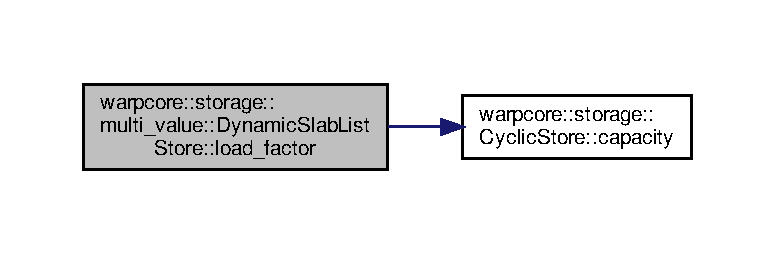
\includegraphics[width=350pt]{classwarpcore_1_1storage_1_1multi__value_1_1DynamicSlabListStore_ab9e38febbac249da5662580311a76f06_cgraph}
\end{center}
\end{figure}
\mbox{\Hypertarget{classwarpcore_1_1storage_1_1multi__value_1_1DynamicSlabListStore_a58f11e19acf684db903b7985364ec73c}\label{classwarpcore_1_1storage_1_1multi__value_1_1DynamicSlabListStore_a58f11e19acf684db903b7985364ec73c}} 
\index{warpcore\+::storage\+::multi\+\_\+value\+::\+Dynamic\+Slab\+List\+Store@{warpcore\+::storage\+::multi\+\_\+value\+::\+Dynamic\+Slab\+List\+Store}!max\+\_\+slab\+\_\+size@{max\+\_\+slab\+\_\+size}}
\index{max\+\_\+slab\+\_\+size@{max\+\_\+slab\+\_\+size}!warpcore\+::storage\+::multi\+\_\+value\+::\+Dynamic\+Slab\+List\+Store@{warpcore\+::storage\+::multi\+\_\+value\+::\+Dynamic\+Slab\+List\+Store}}
\subsubsection{\texorpdfstring{max\+\_\+slab\+\_\+size()}{max\_slab\_size()}}
{\footnotesize\ttfamily template$<$class Value , index\+\_\+t Slab\+Index\+Bits = 30, index\+\_\+t Value\+Counter\+Bits = 22, index\+\_\+t Slab\+Size\+Bits = 10$>$ \\
\+\_\+\+\_\+host\+\_\+\+\_\+\+\_\+\+\_\+device\+\_\+\+\_\+ index\+\_\+type \hyperlink{classwarpcore_1_1storage_1_1multi__value_1_1DynamicSlabListStore}{warpcore\+::storage\+::multi\+\_\+value\+::\+Dynamic\+Slab\+List\+Store}$<$ Value, Slab\+Index\+Bits, Value\+Counter\+Bits, Slab\+Size\+Bits $>$\+::max\+\_\+slab\+\_\+size (\begin{DoxyParamCaption}{ }\end{DoxyParamCaption}) const\hspace{0.3cm}{\ttfamily [inline]}, {\ttfamily [noexcept]}}



get maximum slab capacity 

\begin{DoxyReturn}{Returns}
capacity 
\end{DoxyReturn}
\mbox{\Hypertarget{classwarpcore_1_1storage_1_1multi__value_1_1DynamicSlabListStore_adb7da0e5836a0274de92f906acaf7a43}\label{classwarpcore_1_1storage_1_1multi__value_1_1DynamicSlabListStore_adb7da0e5836a0274de92f906acaf7a43}} 
\index{warpcore\+::storage\+::multi\+\_\+value\+::\+Dynamic\+Slab\+List\+Store@{warpcore\+::storage\+::multi\+\_\+value\+::\+Dynamic\+Slab\+List\+Store}!min\+\_\+slab\+\_\+size@{min\+\_\+slab\+\_\+size}}
\index{min\+\_\+slab\+\_\+size@{min\+\_\+slab\+\_\+size}!warpcore\+::storage\+::multi\+\_\+value\+::\+Dynamic\+Slab\+List\+Store@{warpcore\+::storage\+::multi\+\_\+value\+::\+Dynamic\+Slab\+List\+Store}}
\subsubsection{\texorpdfstring{min\+\_\+slab\+\_\+size()}{min\_slab\_size()}}
{\footnotesize\ttfamily template$<$class Value , index\+\_\+t Slab\+Index\+Bits = 30, index\+\_\+t Value\+Counter\+Bits = 22, index\+\_\+t Slab\+Size\+Bits = 10$>$ \\
\+\_\+\+\_\+host\+\_\+\+\_\+\+\_\+\+\_\+device\+\_\+\+\_\+ index\+\_\+type \hyperlink{classwarpcore_1_1storage_1_1multi__value_1_1DynamicSlabListStore}{warpcore\+::storage\+::multi\+\_\+value\+::\+Dynamic\+Slab\+List\+Store}$<$ Value, Slab\+Index\+Bits, Value\+Counter\+Bits, Slab\+Size\+Bits $>$\+::min\+\_\+slab\+\_\+size (\begin{DoxyParamCaption}{ }\end{DoxyParamCaption}) const\hspace{0.3cm}{\ttfamily [inline]}, {\ttfamily [noexcept]}}



get minimum slab capacity 

\begin{DoxyReturn}{Returns}
capacity 
\end{DoxyReturn}
\mbox{\Hypertarget{classwarpcore_1_1storage_1_1multi__value_1_1DynamicSlabListStore_a79dffb54a0930061383f69bbc769c6d1}\label{classwarpcore_1_1storage_1_1multi__value_1_1DynamicSlabListStore_a79dffb54a0930061383f69bbc769c6d1}} 
\index{warpcore\+::storage\+::multi\+\_\+value\+::\+Dynamic\+Slab\+List\+Store@{warpcore\+::storage\+::multi\+\_\+value\+::\+Dynamic\+Slab\+List\+Store}!size@{size}}
\index{size@{size}!warpcore\+::storage\+::multi\+\_\+value\+::\+Dynamic\+Slab\+List\+Store@{warpcore\+::storage\+::multi\+\_\+value\+::\+Dynamic\+Slab\+List\+Store}}
\subsubsection{\texorpdfstring{size()}{size()}}
{\footnotesize\ttfamily template$<$class Value , index\+\_\+t Slab\+Index\+Bits = 30, index\+\_\+t Value\+Counter\+Bits = 22, index\+\_\+t Slab\+Size\+Bits = 10$>$ \\
static \+\_\+\+\_\+device\+\_\+\+\_\+ constexpr index\+\_\+type \hyperlink{classwarpcore_1_1storage_1_1multi__value_1_1DynamicSlabListStore}{warpcore\+::storage\+::multi\+\_\+value\+::\+Dynamic\+Slab\+List\+Store}$<$ Value, Slab\+Index\+Bits, Value\+Counter\+Bits, Slab\+Size\+Bits $>$\+::size (\begin{DoxyParamCaption}\item[{handle\+\_\+type}]{handle }\end{DoxyParamCaption})\hspace{0.3cm}{\ttfamily [inline]}, {\ttfamily [static]}, {\ttfamily [noexcept]}}



get number of values in slab list 

\begin{DoxyReturn}{Returns}
value count 
\end{DoxyReturn}
\mbox{\Hypertarget{classwarpcore_1_1storage_1_1multi__value_1_1DynamicSlabListStore_a79fb2a41f22cf59f4edf49c3de82d9dd}\label{classwarpcore_1_1storage_1_1multi__value_1_1DynamicSlabListStore_a79fb2a41f22cf59f4edf49c3de82d9dd}} 
\index{warpcore\+::storage\+::multi\+\_\+value\+::\+Dynamic\+Slab\+List\+Store@{warpcore\+::storage\+::multi\+\_\+value\+::\+Dynamic\+Slab\+List\+Store}!slab\+\_\+grow\+\_\+factor@{slab\+\_\+grow\+\_\+factor}}
\index{slab\+\_\+grow\+\_\+factor@{slab\+\_\+grow\+\_\+factor}!warpcore\+::storage\+::multi\+\_\+value\+::\+Dynamic\+Slab\+List\+Store@{warpcore\+::storage\+::multi\+\_\+value\+::\+Dynamic\+Slab\+List\+Store}}
\subsubsection{\texorpdfstring{slab\+\_\+grow\+\_\+factor()}{slab\_grow\_factor()}}
{\footnotesize\ttfamily template$<$class Value , index\+\_\+t Slab\+Index\+Bits = 30, index\+\_\+t Value\+Counter\+Bits = 22, index\+\_\+t Slab\+Size\+Bits = 10$>$ \\
\+\_\+\+\_\+host\+\_\+\+\_\+\+\_\+\+\_\+device\+\_\+\+\_\+ float \hyperlink{classwarpcore_1_1storage_1_1multi__value_1_1DynamicSlabListStore}{warpcore\+::storage\+::multi\+\_\+value\+::\+Dynamic\+Slab\+List\+Store}$<$ Value, Slab\+Index\+Bits, Value\+Counter\+Bits, Slab\+Size\+Bits $>$\+::slab\+\_\+grow\+\_\+factor (\begin{DoxyParamCaption}{ }\end{DoxyParamCaption}) const\hspace{0.3cm}{\ttfamily [inline]}, {\ttfamily [noexcept]}}



get slab growth factor 

\begin{DoxyReturn}{Returns}
factor 
\end{DoxyReturn}
\mbox{\Hypertarget{classwarpcore_1_1storage_1_1multi__value_1_1DynamicSlabListStore_a20efaad0116184429778d736723c30f3}\label{classwarpcore_1_1storage_1_1multi__value_1_1DynamicSlabListStore_a20efaad0116184429778d736723c30f3}} 
\index{warpcore\+::storage\+::multi\+\_\+value\+::\+Dynamic\+Slab\+List\+Store@{warpcore\+::storage\+::multi\+\_\+value\+::\+Dynamic\+Slab\+List\+Store}!slab\+\_\+index\+\_\+bits@{slab\+\_\+index\+\_\+bits}}
\index{slab\+\_\+index\+\_\+bits@{slab\+\_\+index\+\_\+bits}!warpcore\+::storage\+::multi\+\_\+value\+::\+Dynamic\+Slab\+List\+Store@{warpcore\+::storage\+::multi\+\_\+value\+::\+Dynamic\+Slab\+List\+Store}}
\subsubsection{\texorpdfstring{slab\+\_\+index\+\_\+bits()}{slab\_index\_bits()}}
{\footnotesize\ttfamily template$<$class Value , index\+\_\+t Slab\+Index\+Bits = 30, index\+\_\+t Value\+Counter\+Bits = 22, index\+\_\+t Slab\+Size\+Bits = 10$>$ \\
static \+\_\+\+\_\+host\+\_\+\+\_\+\+\_\+\+\_\+device\+\_\+\+\_\+ constexpr index\+\_\+type \hyperlink{classwarpcore_1_1storage_1_1multi__value_1_1DynamicSlabListStore}{warpcore\+::storage\+::multi\+\_\+value\+::\+Dynamic\+Slab\+List\+Store}$<$ Value, Slab\+Index\+Bits, Value\+Counter\+Bits, Slab\+Size\+Bits $>$\+::slab\+\_\+index\+\_\+bits (\begin{DoxyParamCaption}{ }\end{DoxyParamCaption})\hspace{0.3cm}{\ttfamily [inline]}, {\ttfamily [static]}, {\ttfamily [noexcept]}}



get number of bits used to enumerate slabs 

\begin{DoxyReturn}{Returns}
number of bits 
\end{DoxyReturn}
\mbox{\Hypertarget{classwarpcore_1_1storage_1_1multi__value_1_1DynamicSlabListStore_a16f77ea7e30c30b17af19a229464ed42}\label{classwarpcore_1_1storage_1_1multi__value_1_1DynamicSlabListStore_a16f77ea7e30c30b17af19a229464ed42}} 
\index{warpcore\+::storage\+::multi\+\_\+value\+::\+Dynamic\+Slab\+List\+Store@{warpcore\+::storage\+::multi\+\_\+value\+::\+Dynamic\+Slab\+List\+Store}!slab\+\_\+size\+\_\+bits@{slab\+\_\+size\+\_\+bits}}
\index{slab\+\_\+size\+\_\+bits@{slab\+\_\+size\+\_\+bits}!warpcore\+::storage\+::multi\+\_\+value\+::\+Dynamic\+Slab\+List\+Store@{warpcore\+::storage\+::multi\+\_\+value\+::\+Dynamic\+Slab\+List\+Store}}
\subsubsection{\texorpdfstring{slab\+\_\+size\+\_\+bits()}{slab\_size\_bits()}}
{\footnotesize\ttfamily template$<$class Value , index\+\_\+t Slab\+Index\+Bits = 30, index\+\_\+t Value\+Counter\+Bits = 22, index\+\_\+t Slab\+Size\+Bits = 10$>$ \\
static \+\_\+\+\_\+host\+\_\+\+\_\+\+\_\+\+\_\+device\+\_\+\+\_\+ constexpr index\+\_\+type \hyperlink{classwarpcore_1_1storage_1_1multi__value_1_1DynamicSlabListStore}{warpcore\+::storage\+::multi\+\_\+value\+::\+Dynamic\+Slab\+List\+Store}$<$ Value, Slab\+Index\+Bits, Value\+Counter\+Bits, Slab\+Size\+Bits $>$\+::slab\+\_\+size\+\_\+bits (\begin{DoxyParamCaption}{ }\end{DoxyParamCaption})\hspace{0.3cm}{\ttfamily [inline]}, {\ttfamily [static]}, {\ttfamily [noexcept]}}



get number of bits used to hold the value capacity of a slab 

\begin{DoxyReturn}{Returns}
number of bits 
\end{DoxyReturn}
\mbox{\Hypertarget{classwarpcore_1_1storage_1_1multi__value_1_1DynamicSlabListStore_a9f67ef2bd0b072938bce462656b2c8aa}\label{classwarpcore_1_1storage_1_1multi__value_1_1DynamicSlabListStore_a9f67ef2bd0b072938bce462656b2c8aa}} 
\index{warpcore\+::storage\+::multi\+\_\+value\+::\+Dynamic\+Slab\+List\+Store@{warpcore\+::storage\+::multi\+\_\+value\+::\+Dynamic\+Slab\+List\+Store}!status@{status}}
\index{status@{status}!warpcore\+::storage\+::multi\+\_\+value\+::\+Dynamic\+Slab\+List\+Store@{warpcore\+::storage\+::multi\+\_\+value\+::\+Dynamic\+Slab\+List\+Store}}
\subsubsection{\texorpdfstring{status()}{status()}}
{\footnotesize\ttfamily template$<$class Value , index\+\_\+t Slab\+Index\+Bits = 30, index\+\_\+t Value\+Counter\+Bits = 22, index\+\_\+t Slab\+Size\+Bits = 10$>$ \\
\+\_\+\+\_\+host\+\_\+\+\_\+\+\_\+\+\_\+device\+\_\+\+\_\+ \hyperlink{classwarpcore_1_1Status}{status\+\_\+type} \hyperlink{classwarpcore_1_1storage_1_1multi__value_1_1DynamicSlabListStore}{warpcore\+::storage\+::multi\+\_\+value\+::\+Dynamic\+Slab\+List\+Store}$<$ Value, Slab\+Index\+Bits, Value\+Counter\+Bits, Slab\+Size\+Bits $>$\+::status (\begin{DoxyParamCaption}{ }\end{DoxyParamCaption}) const\hspace{0.3cm}{\ttfamily [inline]}, {\ttfamily [noexcept]}}



get status 

\begin{DoxyReturn}{Returns}
status 
\end{DoxyReturn}
\mbox{\Hypertarget{classwarpcore_1_1storage_1_1multi__value_1_1DynamicSlabListStore_a647790aa072589d7296b7ea57436f297}\label{classwarpcore_1_1storage_1_1multi__value_1_1DynamicSlabListStore_a647790aa072589d7296b7ea57436f297}} 
\index{warpcore\+::storage\+::multi\+\_\+value\+::\+Dynamic\+Slab\+List\+Store@{warpcore\+::storage\+::multi\+\_\+value\+::\+Dynamic\+Slab\+List\+Store}!uninitialized\+\_\+handle@{uninitialized\+\_\+handle}}
\index{uninitialized\+\_\+handle@{uninitialized\+\_\+handle}!warpcore\+::storage\+::multi\+\_\+value\+::\+Dynamic\+Slab\+List\+Store@{warpcore\+::storage\+::multi\+\_\+value\+::\+Dynamic\+Slab\+List\+Store}}
\subsubsection{\texorpdfstring{uninitialized\+\_\+handle()}{uninitialized\_handle()}}
{\footnotesize\ttfamily template$<$class Value , index\+\_\+t Slab\+Index\+Bits = 30, index\+\_\+t Value\+Counter\+Bits = 22, index\+\_\+t Slab\+Size\+Bits = 10$>$ \\
static \+\_\+\+\_\+host\+\_\+\+\_\+\+\_\+\+\_\+device\+\_\+\+\_\+ constexpr handle\+\_\+type \hyperlink{classwarpcore_1_1storage_1_1multi__value_1_1DynamicSlabListStore}{warpcore\+::storage\+::multi\+\_\+value\+::\+Dynamic\+Slab\+List\+Store}$<$ Value, Slab\+Index\+Bits, Value\+Counter\+Bits, Slab\+Size\+Bits $>$\+::uninitialized\+\_\+handle (\begin{DoxyParamCaption}{ }\end{DoxyParamCaption})\hspace{0.3cm}{\ttfamily [inline]}, {\ttfamily [static]}, {\ttfamily [noexcept]}}



get uninitialized handle 

\begin{DoxyReturn}{Returns}
handle 
\end{DoxyReturn}
\mbox{\Hypertarget{classwarpcore_1_1storage_1_1multi__value_1_1DynamicSlabListStore_aff75cc3f371c2b31b569ff585f9ac900}\label{classwarpcore_1_1storage_1_1multi__value_1_1DynamicSlabListStore_aff75cc3f371c2b31b569ff585f9ac900}} 
\index{warpcore\+::storage\+::multi\+\_\+value\+::\+Dynamic\+Slab\+List\+Store@{warpcore\+::storage\+::multi\+\_\+value\+::\+Dynamic\+Slab\+List\+Store}!value\+\_\+counter\+\_\+bits@{value\+\_\+counter\+\_\+bits}}
\index{value\+\_\+counter\+\_\+bits@{value\+\_\+counter\+\_\+bits}!warpcore\+::storage\+::multi\+\_\+value\+::\+Dynamic\+Slab\+List\+Store@{warpcore\+::storage\+::multi\+\_\+value\+::\+Dynamic\+Slab\+List\+Store}}
\subsubsection{\texorpdfstring{value\+\_\+counter\+\_\+bits()}{value\_counter\_bits()}}
{\footnotesize\ttfamily template$<$class Value , index\+\_\+t Slab\+Index\+Bits = 30, index\+\_\+t Value\+Counter\+Bits = 22, index\+\_\+t Slab\+Size\+Bits = 10$>$ \\
static \+\_\+\+\_\+host\+\_\+\+\_\+\+\_\+\+\_\+device\+\_\+\+\_\+ constexpr index\+\_\+type \hyperlink{classwarpcore_1_1storage_1_1multi__value_1_1DynamicSlabListStore}{warpcore\+::storage\+::multi\+\_\+value\+::\+Dynamic\+Slab\+List\+Store}$<$ Value, Slab\+Index\+Bits, Value\+Counter\+Bits, Slab\+Size\+Bits $>$\+::value\+\_\+counter\+\_\+bits (\begin{DoxyParamCaption}{ }\end{DoxyParamCaption})\hspace{0.3cm}{\ttfamily [inline]}, {\ttfamily [static]}, {\ttfamily [noexcept]}}



get number of bits used to count values in a slab list 

\begin{DoxyReturn}{Returns}
number of bits 
\end{DoxyReturn}

\hypertarget{classwarpcore_1_1HashSet}{}\doxysection{warpcore\+::Hash\+Set$<$ Key, Empty\+Key, Tombstone\+Key, Probing\+Scheme, Temp\+Memory\+Bytes $>$ Class Template Reference}
\label{classwarpcore_1_1HashSet}\index{warpcore::HashSet$<$ Key, EmptyKey, TombstoneKey, ProbingScheme, TempMemoryBytes $>$@{warpcore::HashSet$<$ Key, EmptyKey, TombstoneKey, ProbingScheme, TempMemoryBytes $>$}}


hash set  


\doxysubsection*{Public Types}
\begin{DoxyCompactItemize}
\item 
\mbox{\Hypertarget{classwarpcore_1_1HashSet_a63b9dab14e325289f3291c9c70acb61f}\label{classwarpcore_1_1HashSet_a63b9dab14e325289f3291c9c70acb61f}} 
using {\bfseries key\+\_\+type} = Key
\item 
\mbox{\Hypertarget{classwarpcore_1_1HashSet_a676d14c28ab3a6c6c80c2a626d168930}\label{classwarpcore_1_1HashSet_a676d14c28ab3a6c6c80c2a626d168930}} 
using {\bfseries index\+\_\+type} = index\+\_\+t
\item 
\mbox{\Hypertarget{classwarpcore_1_1HashSet_a0bb489daa2ebec41b5e7df445cb55a51}\label{classwarpcore_1_1HashSet_a0bb489daa2ebec41b5e7df445cb55a51}} 
using {\bfseries status\+\_\+type} = \mbox{\hyperlink{classwarpcore_1_1Status}{Status}}
\end{DoxyCompactItemize}
\doxysubsection*{Public Member Functions}
\begin{DoxyCompactItemize}
\item 
\+\_\+\+\_\+host\+\_\+\+\_\+ \mbox{\hyperlink{classwarpcore_1_1HashSet_aff2bcd0720090d1dcfc03d0e7d9a1eab}{Hash\+Set}} (index\+\_\+type min\+\_\+capacity, key\+\_\+type seed=defaults\+::seed$<$ key\+\_\+type $>$()) noexcept
\begin{DoxyCompactList}\small\item\em constructor \end{DoxyCompactList}\item 
\+\_\+\+\_\+host\+\_\+\+\_\+\+\_\+\+\_\+device\+\_\+\+\_\+ \mbox{\hyperlink{classwarpcore_1_1HashSet_a4f3bde62cd45155bbc7eb5db38357f28}{Hash\+Set}} (const \mbox{\hyperlink{classwarpcore_1_1HashSet}{Hash\+Set}} \&o) noexcept
\begin{DoxyCompactList}\small\item\em copy-\/constructor (shallow) \end{DoxyCompactList}\item 
\+\_\+\+\_\+host\+\_\+\+\_\+ \mbox{\hyperlink{classwarpcore_1_1HashSet_a572b36003a5652fa6a28155b9a5b6e1d}{Hash\+Set}} (\mbox{\hyperlink{classwarpcore_1_1HashSet}{Hash\+Set}} \&\&o) noexcept
\begin{DoxyCompactList}\small\item\em move-\/constructor \end{DoxyCompactList}\item 
\mbox{\Hypertarget{classwarpcore_1_1HashSet_a5419d12a6675f108bcda8a03580ee67c}\label{classwarpcore_1_1HashSet_a5419d12a6675f108bcda8a03580ee67c}} 
\+\_\+\+\_\+host\+\_\+\+\_\+ \mbox{\hyperlink{classwarpcore_1_1HashSet_a5419d12a6675f108bcda8a03580ee67c}{$\sim$\+Hash\+Set}} () noexcept
\begin{DoxyCompactList}\small\item\em destructor \end{DoxyCompactList}\item 
\+\_\+\+\_\+host\+\_\+\+\_\+ void \mbox{\hyperlink{classwarpcore_1_1HashSet_a6654bf5c2c17b0676d6fd4867fa991cd}{init}} (const key\+\_\+type seed, const cuda\+Stream\+\_\+t stream=0) noexcept
\begin{DoxyCompactList}\small\item\em (re)initialize the hash set \end{DoxyCompactList}\item 
\+\_\+\+\_\+host\+\_\+\+\_\+ void \mbox{\hyperlink{classwarpcore_1_1HashSet_ae21bfb96f28d7b097841d6a6874c16d5}{init}} (const cuda\+Stream\+\_\+t stream=0) noexcept
\begin{DoxyCompactList}\small\item\em (re)initialize the hash set \end{DoxyCompactList}\item 
\+\_\+\+\_\+device\+\_\+\+\_\+ \mbox{\hyperlink{classwarpcore_1_1Status}{Status}} \mbox{\hyperlink{classwarpcore_1_1HashSet_af54d9aecfefb13e451e0580a38702f54}{insert}} (key\+\_\+type key\+\_\+in, const cg\+::thread\+\_\+block\+\_\+tile$<$ \mbox{\hyperlink{classwarpcore_1_1HashSet_ae1eccbda8dec86180c8798e16e6ff00d}{cg\+\_\+size}}()$>$ \&group, index\+\_\+type probing\+\_\+length=defaults\+::probing\+\_\+length()) noexcept
\begin{DoxyCompactList}\small\item\em inserts a key into the hash set \end{DoxyCompactList}\item 
{\footnotesize template$<$class Status\+Handler  = defaults\+::status\+\_\+handler\+\_\+t$>$ }\\\+\_\+\+\_\+host\+\_\+\+\_\+ void \mbox{\hyperlink{classwarpcore_1_1HashSet_aa5f8752a439792aa532d04abb50b0f26}{insert}} (key\+\_\+type $\ast$keys\+\_\+in, index\+\_\+type num\+\_\+in, cuda\+Stream\+\_\+t stream=0, index\+\_\+type probing\+\_\+length=defaults\+::probing\+\_\+length(), typename Status\+Handler\+::base\+\_\+type $\ast$status\+\_\+out=nullptr) noexcept
\begin{DoxyCompactList}\small\item\em insert a set of keys into the hash set \end{DoxyCompactList}\item 
\+\_\+\+\_\+device\+\_\+\+\_\+ \mbox{\hyperlink{classwarpcore_1_1Status}{Status}} \mbox{\hyperlink{classwarpcore_1_1HashSet_a3be33bdea6aabe4075b7e6f9a3741021}{retrieve}} (Key key\+\_\+in, bool \&flag\+\_\+out, const cg\+::thread\+\_\+block\+\_\+tile$<$ \mbox{\hyperlink{classwarpcore_1_1HashSet_ae1eccbda8dec86180c8798e16e6ff00d}{cg\+\_\+size}}()$>$ \&group, index\+\_\+type probing\+\_\+length=defaults\+::probing\+\_\+length()) const noexcept
\begin{DoxyCompactList}\small\item\em retrieves a key from the hash set \end{DoxyCompactList}\item 
{\footnotesize template$<$class Status\+Handler  = defaults\+::status\+\_\+handler\+\_\+t$>$ }\\\+\_\+\+\_\+host\+\_\+\+\_\+ void \mbox{\hyperlink{classwarpcore_1_1HashSet_a0012b8162ac192387bafc44bc773f70a}{retrieve}} (key\+\_\+type $\ast$keys\+\_\+in, index\+\_\+type num\+\_\+in, bool $\ast$flags\+\_\+out, cuda\+Stream\+\_\+t stream=0, index\+\_\+type probing\+\_\+length=defaults\+::probing\+\_\+length(), typename Status\+Handler\+::base\+\_\+type $\ast$status\+\_\+out=nullptr) const noexcept
\begin{DoxyCompactList}\small\item\em retrieve a set of keys from the hash table \end{DoxyCompactList}\item 
\+\_\+\+\_\+host\+\_\+\+\_\+ void \mbox{\hyperlink{classwarpcore_1_1HashSet_a6a178adc0aac5636950e84134bc851cc}{retrieve\+\_\+all}} (key\+\_\+type $\ast$keys\+\_\+out, index\+\_\+type \&num\+\_\+out, cuda\+Stream\+\_\+t stream=0) const noexcept
\begin{DoxyCompactList}\small\item\em retrieves all elements from the hash set \end{DoxyCompactList}\item 
\+\_\+\+\_\+device\+\_\+\+\_\+ \mbox{\hyperlink{classwarpcore_1_1Status}{Status}} \mbox{\hyperlink{classwarpcore_1_1HashSet_a255b77ba7f1ba8a1faabddfd92ae976c}{erase}} (key\+\_\+type key\+\_\+in, const cg\+::thread\+\_\+block\+\_\+tile$<$ \mbox{\hyperlink{classwarpcore_1_1HashSet_ae1eccbda8dec86180c8798e16e6ff00d}{cg\+\_\+size}}()$>$ \&group, index\+\_\+type probing\+\_\+length=defaults\+::probing\+\_\+length()) noexcept
\begin{DoxyCompactList}\small\item\em erases a key from the hash table \end{DoxyCompactList}\item 
{\footnotesize template$<$class Status\+Handler  = defaults\+::status\+\_\+handler\+\_\+t$>$ }\\\+\_\+\+\_\+host\+\_\+\+\_\+ void \mbox{\hyperlink{classwarpcore_1_1HashSet_a0480bc6e9197ccc13a50155d830adfb4}{erase}} (key\+\_\+type $\ast$keys\+\_\+in, index\+\_\+type num\+\_\+in, cuda\+Stream\+\_\+t stream=0, index\+\_\+type probing\+\_\+length=defaults\+::probing\+\_\+length(), typename Status\+Handler\+::base\+\_\+type $\ast$status\+\_\+out=nullptr) noexcept
\begin{DoxyCompactList}\small\item\em erases a set of keys from the hash table \end{DoxyCompactList}\item 
{\footnotesize template$<$class Func $>$ }\\\+\_\+\+\_\+host\+\_\+\+\_\+ void \mbox{\hyperlink{classwarpcore_1_1HashSet_a8719aee40fca90a39085ac0253bbdd01}{for\+\_\+each}} (Func f, cuda\+Stream\+\_\+t stream=0, index\+\_\+type smem\+\_\+bytes=0) const noexcept
\begin{DoxyCompactList}\small\item\em applies a funtion on all keys inside the table \end{DoxyCompactList}\item 
\+\_\+\+\_\+host\+\_\+\+\_\+ index\+\_\+type \mbox{\hyperlink{classwarpcore_1_1HashSet_a06649688aa7e9f6538965f1dec18c82b}{size}} (cuda\+Stream\+\_\+t stream=0) const noexcept
\begin{DoxyCompactList}\small\item\em number of key/value pairs stored inside the hash set \end{DoxyCompactList}\item 
\+\_\+\+\_\+host\+\_\+\+\_\+ float \mbox{\hyperlink{classwarpcore_1_1HashSet_a7ad4ad097ae0e332c4f24d867e6c411f}{load\+\_\+factor}} (cuda\+Stream\+\_\+t stream=0) const noexcept
\begin{DoxyCompactList}\small\item\em current load factor of the hash set \end{DoxyCompactList}\item 
\+\_\+\+\_\+host\+\_\+\+\_\+ float \mbox{\hyperlink{classwarpcore_1_1HashSet_a178dec74a9404d6b89f37febec381dca}{storage\+\_\+density}} (cuda\+Stream\+\_\+t stream=0) const noexcept
\begin{DoxyCompactList}\small\item\em current storage density of the hash set \end{DoxyCompactList}\item 
\+\_\+\+\_\+host\+\_\+\+\_\+\+\_\+\+\_\+device\+\_\+\+\_\+ index\+\_\+type \mbox{\hyperlink{classwarpcore_1_1HashSet_a6edef2d260c214f294b61bb394a11545}{capacity}} () const noexcept
\begin{DoxyCompactList}\small\item\em get the capacity of the hash table \end{DoxyCompactList}\item 
\+\_\+\+\_\+host\+\_\+\+\_\+ index\+\_\+type \mbox{\hyperlink{classwarpcore_1_1HashSet_a64aa9503fa5719a2d91bf9ecf2aa3cdc}{bytes\+\_\+total}} () const noexcept
\begin{DoxyCompactList}\small\item\em get the total number of bytes occupied by this data structure \end{DoxyCompactList}\item 
\+\_\+\+\_\+host\+\_\+\+\_\+ \mbox{\hyperlink{classwarpcore_1_1Status}{Status}} \mbox{\hyperlink{classwarpcore_1_1HashSet_a15b81a16c6fbdb88dee1fd8c05a9fdbd}{peek\+\_\+status}} (cuda\+Stream\+\_\+t stream=0) const noexcept
\begin{DoxyCompactList}\small\item\em get the status of the hash table \end{DoxyCompactList}\item 
\+\_\+\+\_\+host\+\_\+\+\_\+ \mbox{\hyperlink{classwarpcore_1_1Status}{Status}} \mbox{\hyperlink{classwarpcore_1_1HashSet_ae9a6c692c64bbc40bb6abd3372b946d1}{pop\+\_\+status}} (cuda\+Stream\+\_\+t stream=0) noexcept
\begin{DoxyCompactList}\small\item\em get and reset the status of the hash table \end{DoxyCompactList}\item 
\+\_\+\+\_\+host\+\_\+\+\_\+\+\_\+\+\_\+device\+\_\+\+\_\+ bool \mbox{\hyperlink{classwarpcore_1_1HashSet_ac1b20d9d5305bbd8e7fca93aa580c984}{is\+\_\+copy}} () const noexcept
\begin{DoxyCompactList}\small\item\em indicates if this object is a shallow copy \end{DoxyCompactList}\end{DoxyCompactItemize}
\doxysubsection*{Static Public Member Functions}
\begin{DoxyCompactItemize}
\item 
static constexpr \+\_\+\+\_\+host\+\_\+\+\_\+\+\_\+\+\_\+device\+\_\+\+\_\+ key\+\_\+type \mbox{\hyperlink{classwarpcore_1_1HashSet_ab28ac96cb8e02dd35b2ba73334175ab7}{empty\+\_\+key}} () noexcept
\begin{DoxyCompactList}\small\item\em get empty key \end{DoxyCompactList}\item 
static constexpr \+\_\+\+\_\+host\+\_\+\+\_\+\+\_\+\+\_\+device\+\_\+\+\_\+ key\+\_\+type \mbox{\hyperlink{classwarpcore_1_1HashSet_a6e23aa0327da71ca30454d5a4815064e}{tombstone\+\_\+key}} () noexcept
\begin{DoxyCompactList}\small\item\em get tombstone key \end{DoxyCompactList}\item 
static constexpr \+\_\+\+\_\+host\+\_\+\+\_\+\+\_\+\+\_\+device\+\_\+\+\_\+ index\+\_\+type \mbox{\hyperlink{classwarpcore_1_1HashSet_ae1eccbda8dec86180c8798e16e6ff00d}{cg\+\_\+size}} () noexcept
\begin{DoxyCompactList}\small\item\em get cooperative group size \end{DoxyCompactList}\item 
static constexpr \+\_\+\+\_\+host\+\_\+\+\_\+\+\_\+\+\_\+device\+\_\+\+\_\+ bool \mbox{\hyperlink{classwarpcore_1_1HashSet_af07ed139aa043222f6f25058cf7c53e2}{is\+\_\+empty\+\_\+key}} (key\+\_\+type key) noexcept
\begin{DoxyCompactList}\small\item\em checks if {\ttfamily key} is equal to {\ttfamily Empty\+Key} \end{DoxyCompactList}\item 
static constexpr \+\_\+\+\_\+host\+\_\+\+\_\+\+\_\+\+\_\+device\+\_\+\+\_\+ bool \mbox{\hyperlink{classwarpcore_1_1HashSet_a41943b97bab382d38d17b7b222907f80}{is\+\_\+tombstone\+\_\+key}} (key\+\_\+type key) noexcept
\begin{DoxyCompactList}\small\item\em checks if {\ttfamily key} is equal to {\ttfamily Tombstone\+Key} \end{DoxyCompactList}\item 
static constexpr \+\_\+\+\_\+host\+\_\+\+\_\+\+\_\+\+\_\+device\+\_\+\+\_\+ bool \mbox{\hyperlink{classwarpcore_1_1HashSet_aeec18cd128763576033aab044471ffa7}{is\+\_\+valid\+\_\+key}} (key\+\_\+type key) noexcept
\begin{DoxyCompactList}\small\item\em checks if {\ttfamily key} is equal to {\ttfamily }(Empty\+Key$\vert$$\vert$\+Tombstone\+Key) \end{DoxyCompactList}\end{DoxyCompactItemize}


\doxysubsection{Detailed Description}
\subsubsection*{template$<$class Key, Key Empty\+Key = defaults\+::empty\+\_\+key$<$\+Key$>$(), Key Tombstone\+Key = defaults\+::tombstone\+\_\+key$<$\+Key$>$(), class Probing\+Scheme = defaults\+::probing\+\_\+scheme\+\_\+t$<$\+Key, 16$>$, index\+\_\+t Temp\+Memory\+Bytes = defaults\+::temp\+\_\+memory\+\_\+bytes()$>$\newline
class warpcore\+::\+Hash\+Set$<$ Key, Empty\+Key, Tombstone\+Key, Probing\+Scheme, Temp\+Memory\+Bytes $>$}

hash set 


\begin{DoxyTemplParams}{Template Parameters}
{\em Key} & key type ({\ttfamily std\+::uint32\+\_\+t} or {\ttfamily std\+::uint64\+\_\+t}) \\
\hline
{\em Empty\+Key} & key which represents an empty slot \\
\hline
{\em Tombstone\+Key} & key which represents an erased slot \\
\hline
{\em Probing\+Scheme} & probing scheme from {\ttfamily \mbox{\hyperlink{namespacewarpcore_1_1probing__schemes}{warpcore\+::probing\+\_\+schemes}}} \\
\hline
{\em Temp\+Memory\+Bytes} & size of temporary storage (typically a few kB) \\
\hline
\end{DoxyTemplParams}


\doxysubsection{Constructor \& Destructor Documentation}
\mbox{\Hypertarget{classwarpcore_1_1HashSet_aff2bcd0720090d1dcfc03d0e7d9a1eab}\label{classwarpcore_1_1HashSet_aff2bcd0720090d1dcfc03d0e7d9a1eab}} 
\index{warpcore::HashSet$<$ Key, EmptyKey, TombstoneKey, ProbingScheme, TempMemoryBytes $>$@{warpcore::HashSet$<$ Key, EmptyKey, TombstoneKey, ProbingScheme, TempMemoryBytes $>$}!HashSet@{HashSet}}
\index{HashSet@{HashSet}!warpcore::HashSet$<$ Key, EmptyKey, TombstoneKey, ProbingScheme, TempMemoryBytes $>$@{warpcore::HashSet$<$ Key, EmptyKey, TombstoneKey, ProbingScheme, TempMemoryBytes $>$}}
\doxysubsubsection{\texorpdfstring{HashSet()}{HashSet()}\hspace{0.1cm}{\footnotesize\ttfamily [1/3]}}
{\footnotesize\ttfamily template$<$class Key , Key Empty\+Key = defaults\+::empty\+\_\+key$<$\+Key$>$(), Key Tombstone\+Key = defaults\+::tombstone\+\_\+key$<$\+Key$>$(), class Probing\+Scheme  = defaults\+::probing\+\_\+scheme\+\_\+t$<$\+Key, 16$>$, index\+\_\+t Temp\+Memory\+Bytes = defaults\+::temp\+\_\+memory\+\_\+bytes()$>$ \\
\+\_\+\+\_\+host\+\_\+\+\_\+ \mbox{\hyperlink{classwarpcore_1_1HashSet}{warpcore\+::\+Hash\+Set}}$<$ Key, Empty\+Key, Tombstone\+Key, Probing\+Scheme, Temp\+Memory\+Bytes $>$\+::\mbox{\hyperlink{classwarpcore_1_1HashSet}{Hash\+Set}} (\begin{DoxyParamCaption}\item[{index\+\_\+type}]{min\+\_\+capacity,  }\item[{key\+\_\+type}]{seed = {\ttfamily defaults\+:\+:seed$<$key\+\_\+type$>$()} }\end{DoxyParamCaption})\hspace{0.3cm}{\ttfamily [inline]}, {\ttfamily [explicit]}, {\ttfamily [noexcept]}}



constructor 


\begin{DoxyParams}[1]{Parameters}
\mbox{\texttt{ in}}  & {\em capacity} & maximum cardinality of the set \\
\hline
\mbox{\texttt{ in}}  & {\em seed} & random seed \\
\hline
\end{DoxyParams}
Here is the call graph for this function\+:
\nopagebreak
\begin{figure}[H]
\begin{center}
\leavevmode
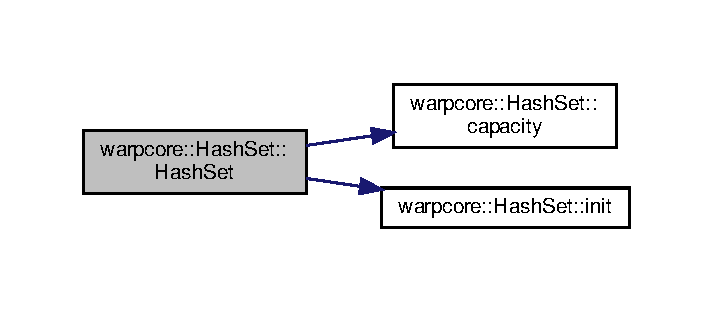
\includegraphics[width=350pt]{classwarpcore_1_1HashSet_aff2bcd0720090d1dcfc03d0e7d9a1eab_cgraph}
\end{center}
\end{figure}
\mbox{\Hypertarget{classwarpcore_1_1HashSet_a4f3bde62cd45155bbc7eb5db38357f28}\label{classwarpcore_1_1HashSet_a4f3bde62cd45155bbc7eb5db38357f28}} 
\index{warpcore::HashSet$<$ Key, EmptyKey, TombstoneKey, ProbingScheme, TempMemoryBytes $>$@{warpcore::HashSet$<$ Key, EmptyKey, TombstoneKey, ProbingScheme, TempMemoryBytes $>$}!HashSet@{HashSet}}
\index{HashSet@{HashSet}!warpcore::HashSet$<$ Key, EmptyKey, TombstoneKey, ProbingScheme, TempMemoryBytes $>$@{warpcore::HashSet$<$ Key, EmptyKey, TombstoneKey, ProbingScheme, TempMemoryBytes $>$}}
\doxysubsubsection{\texorpdfstring{HashSet()}{HashSet()}\hspace{0.1cm}{\footnotesize\ttfamily [2/3]}}
{\footnotesize\ttfamily template$<$class Key , Key Empty\+Key = defaults\+::empty\+\_\+key$<$\+Key$>$(), Key Tombstone\+Key = defaults\+::tombstone\+\_\+key$<$\+Key$>$(), class Probing\+Scheme  = defaults\+::probing\+\_\+scheme\+\_\+t$<$\+Key, 16$>$, index\+\_\+t Temp\+Memory\+Bytes = defaults\+::temp\+\_\+memory\+\_\+bytes()$>$ \\
\+\_\+\+\_\+host\+\_\+\+\_\+\+\_\+\+\_\+device\+\_\+\+\_\+ \mbox{\hyperlink{classwarpcore_1_1HashSet}{warpcore\+::\+Hash\+Set}}$<$ Key, Empty\+Key, Tombstone\+Key, Probing\+Scheme, Temp\+Memory\+Bytes $>$\+::\mbox{\hyperlink{classwarpcore_1_1HashSet}{Hash\+Set}} (\begin{DoxyParamCaption}\item[{const \mbox{\hyperlink{classwarpcore_1_1HashSet}{Hash\+Set}}$<$ Key, Empty\+Key, Tombstone\+Key, Probing\+Scheme, Temp\+Memory\+Bytes $>$ \&}]{o }\end{DoxyParamCaption})\hspace{0.3cm}{\ttfamily [inline]}, {\ttfamily [noexcept]}}



copy-\/constructor (shallow) 


\begin{DoxyParams}[1]{Parameters}
\mbox{\texttt{ in}}  & {\em object} & to be copied \\
\hline
\end{DoxyParams}
\mbox{\Hypertarget{classwarpcore_1_1HashSet_a572b36003a5652fa6a28155b9a5b6e1d}\label{classwarpcore_1_1HashSet_a572b36003a5652fa6a28155b9a5b6e1d}} 
\index{warpcore::HashSet$<$ Key, EmptyKey, TombstoneKey, ProbingScheme, TempMemoryBytes $>$@{warpcore::HashSet$<$ Key, EmptyKey, TombstoneKey, ProbingScheme, TempMemoryBytes $>$}!HashSet@{HashSet}}
\index{HashSet@{HashSet}!warpcore::HashSet$<$ Key, EmptyKey, TombstoneKey, ProbingScheme, TempMemoryBytes $>$@{warpcore::HashSet$<$ Key, EmptyKey, TombstoneKey, ProbingScheme, TempMemoryBytes $>$}}
\doxysubsubsection{\texorpdfstring{HashSet()}{HashSet()}\hspace{0.1cm}{\footnotesize\ttfamily [3/3]}}
{\footnotesize\ttfamily template$<$class Key , Key Empty\+Key = defaults\+::empty\+\_\+key$<$\+Key$>$(), Key Tombstone\+Key = defaults\+::tombstone\+\_\+key$<$\+Key$>$(), class Probing\+Scheme  = defaults\+::probing\+\_\+scheme\+\_\+t$<$\+Key, 16$>$, index\+\_\+t Temp\+Memory\+Bytes = defaults\+::temp\+\_\+memory\+\_\+bytes()$>$ \\
\+\_\+\+\_\+host\+\_\+\+\_\+ \mbox{\hyperlink{classwarpcore_1_1HashSet}{warpcore\+::\+Hash\+Set}}$<$ Key, Empty\+Key, Tombstone\+Key, Probing\+Scheme, Temp\+Memory\+Bytes $>$\+::\mbox{\hyperlink{classwarpcore_1_1HashSet}{Hash\+Set}} (\begin{DoxyParamCaption}\item[{\mbox{\hyperlink{classwarpcore_1_1HashSet}{Hash\+Set}}$<$ Key, Empty\+Key, Tombstone\+Key, Probing\+Scheme, Temp\+Memory\+Bytes $>$ \&\&}]{o }\end{DoxyParamCaption})\hspace{0.3cm}{\ttfamily [inline]}, {\ttfamily [noexcept]}}



move-\/constructor 


\begin{DoxyParams}[1]{Parameters}
\mbox{\texttt{ in}}  & {\em object} & to be moved \\
\hline
\end{DoxyParams}


\doxysubsection{Member Function Documentation}
\mbox{\Hypertarget{classwarpcore_1_1HashSet_a64aa9503fa5719a2d91bf9ecf2aa3cdc}\label{classwarpcore_1_1HashSet_a64aa9503fa5719a2d91bf9ecf2aa3cdc}} 
\index{warpcore::HashSet$<$ Key, EmptyKey, TombstoneKey, ProbingScheme, TempMemoryBytes $>$@{warpcore::HashSet$<$ Key, EmptyKey, TombstoneKey, ProbingScheme, TempMemoryBytes $>$}!bytes\_total@{bytes\_total}}
\index{bytes\_total@{bytes\_total}!warpcore::HashSet$<$ Key, EmptyKey, TombstoneKey, ProbingScheme, TempMemoryBytes $>$@{warpcore::HashSet$<$ Key, EmptyKey, TombstoneKey, ProbingScheme, TempMemoryBytes $>$}}
\doxysubsubsection{\texorpdfstring{bytes\_total()}{bytes\_total()}}
{\footnotesize\ttfamily template$<$class Key , Key Empty\+Key = defaults\+::empty\+\_\+key$<$\+Key$>$(), Key Tombstone\+Key = defaults\+::tombstone\+\_\+key$<$\+Key$>$(), class Probing\+Scheme  = defaults\+::probing\+\_\+scheme\+\_\+t$<$\+Key, 16$>$, index\+\_\+t Temp\+Memory\+Bytes = defaults\+::temp\+\_\+memory\+\_\+bytes()$>$ \\
\+\_\+\+\_\+host\+\_\+\+\_\+ index\+\_\+type \mbox{\hyperlink{classwarpcore_1_1HashSet}{warpcore\+::\+Hash\+Set}}$<$ Key, Empty\+Key, Tombstone\+Key, Probing\+Scheme, Temp\+Memory\+Bytes $>$\+::bytes\+\_\+total (\begin{DoxyParamCaption}{ }\end{DoxyParamCaption}) const\hspace{0.3cm}{\ttfamily [inline]}, {\ttfamily [noexcept]}}



get the total number of bytes occupied by this data structure 

\begin{DoxyReturn}{Returns}
bytes 
\end{DoxyReturn}
Here is the call graph for this function\+:
\nopagebreak
\begin{figure}[H]
\begin{center}
\leavevmode
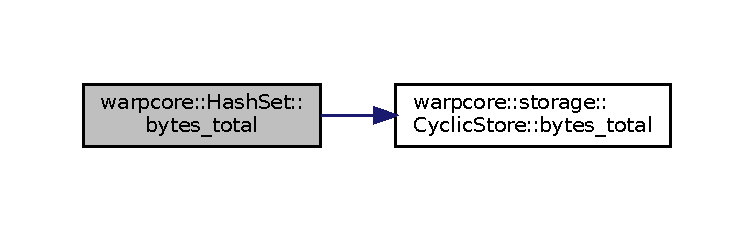
\includegraphics[width=350pt]{classwarpcore_1_1HashSet_a64aa9503fa5719a2d91bf9ecf2aa3cdc_cgraph}
\end{center}
\end{figure}
\mbox{\Hypertarget{classwarpcore_1_1HashSet_a6edef2d260c214f294b61bb394a11545}\label{classwarpcore_1_1HashSet_a6edef2d260c214f294b61bb394a11545}} 
\index{warpcore::HashSet$<$ Key, EmptyKey, TombstoneKey, ProbingScheme, TempMemoryBytes $>$@{warpcore::HashSet$<$ Key, EmptyKey, TombstoneKey, ProbingScheme, TempMemoryBytes $>$}!capacity@{capacity}}
\index{capacity@{capacity}!warpcore::HashSet$<$ Key, EmptyKey, TombstoneKey, ProbingScheme, TempMemoryBytes $>$@{warpcore::HashSet$<$ Key, EmptyKey, TombstoneKey, ProbingScheme, TempMemoryBytes $>$}}
\doxysubsubsection{\texorpdfstring{capacity()}{capacity()}}
{\footnotesize\ttfamily template$<$class Key , Key Empty\+Key = defaults\+::empty\+\_\+key$<$\+Key$>$(), Key Tombstone\+Key = defaults\+::tombstone\+\_\+key$<$\+Key$>$(), class Probing\+Scheme  = defaults\+::probing\+\_\+scheme\+\_\+t$<$\+Key, 16$>$, index\+\_\+t Temp\+Memory\+Bytes = defaults\+::temp\+\_\+memory\+\_\+bytes()$>$ \\
\+\_\+\+\_\+host\+\_\+\+\_\+\+\_\+\+\_\+device\+\_\+\+\_\+ index\+\_\+type \mbox{\hyperlink{classwarpcore_1_1HashSet}{warpcore\+::\+Hash\+Set}}$<$ Key, Empty\+Key, Tombstone\+Key, Probing\+Scheme, Temp\+Memory\+Bytes $>$\+::capacity (\begin{DoxyParamCaption}{ }\end{DoxyParamCaption}) const\hspace{0.3cm}{\ttfamily [inline]}, {\ttfamily [noexcept]}}



get the capacity of the hash table 

\begin{DoxyReturn}{Returns}
number of slots in the hash table 
\end{DoxyReturn}
Here is the caller graph for this function\+:
\nopagebreak
\begin{figure}[H]
\begin{center}
\leavevmode
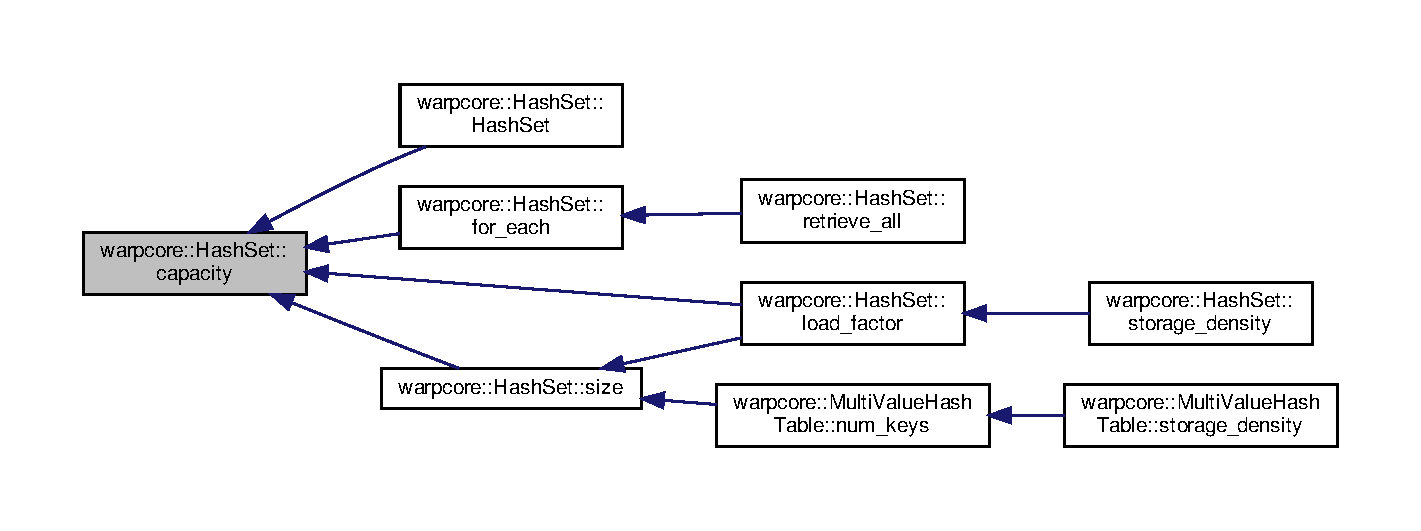
\includegraphics[width=350pt]{classwarpcore_1_1HashSet_a6edef2d260c214f294b61bb394a11545_icgraph}
\end{center}
\end{figure}
\mbox{\Hypertarget{classwarpcore_1_1HashSet_ae1eccbda8dec86180c8798e16e6ff00d}\label{classwarpcore_1_1HashSet_ae1eccbda8dec86180c8798e16e6ff00d}} 
\index{warpcore::HashSet$<$ Key, EmptyKey, TombstoneKey, ProbingScheme, TempMemoryBytes $>$@{warpcore::HashSet$<$ Key, EmptyKey, TombstoneKey, ProbingScheme, TempMemoryBytes $>$}!cg\_size@{cg\_size}}
\index{cg\_size@{cg\_size}!warpcore::HashSet$<$ Key, EmptyKey, TombstoneKey, ProbingScheme, TempMemoryBytes $>$@{warpcore::HashSet$<$ Key, EmptyKey, TombstoneKey, ProbingScheme, TempMemoryBytes $>$}}
\doxysubsubsection{\texorpdfstring{cg\_size()}{cg\_size()}}
{\footnotesize\ttfamily template$<$class Key , Key Empty\+Key = defaults\+::empty\+\_\+key$<$\+Key$>$(), Key Tombstone\+Key = defaults\+::tombstone\+\_\+key$<$\+Key$>$(), class Probing\+Scheme  = defaults\+::probing\+\_\+scheme\+\_\+t$<$\+Key, 16$>$, index\+\_\+t Temp\+Memory\+Bytes = defaults\+::temp\+\_\+memory\+\_\+bytes()$>$ \\
static constexpr \+\_\+\+\_\+host\+\_\+\+\_\+\+\_\+\+\_\+device\+\_\+\+\_\+ index\+\_\+type \mbox{\hyperlink{classwarpcore_1_1HashSet}{warpcore\+::\+Hash\+Set}}$<$ Key, Empty\+Key, Tombstone\+Key, Probing\+Scheme, Temp\+Memory\+Bytes $>$\+::cg\+\_\+size (\begin{DoxyParamCaption}{ }\end{DoxyParamCaption})\hspace{0.3cm}{\ttfamily [inline]}, {\ttfamily [static]}, {\ttfamily [constexpr]}, {\ttfamily [noexcept]}}



get cooperative group size 

\begin{DoxyReturn}{Returns}
cooperative group size 
\end{DoxyReturn}
Here is the caller graph for this function\+:
\nopagebreak
\begin{figure}[H]
\begin{center}
\leavevmode
\includegraphics[width=344pt]{classwarpcore_1_1HashSet_ae1eccbda8dec86180c8798e16e6ff00d_icgraph}
\end{center}
\end{figure}
\mbox{\Hypertarget{classwarpcore_1_1HashSet_ab28ac96cb8e02dd35b2ba73334175ab7}\label{classwarpcore_1_1HashSet_ab28ac96cb8e02dd35b2ba73334175ab7}} 
\index{warpcore::HashSet$<$ Key, EmptyKey, TombstoneKey, ProbingScheme, TempMemoryBytes $>$@{warpcore::HashSet$<$ Key, EmptyKey, TombstoneKey, ProbingScheme, TempMemoryBytes $>$}!empty\_key@{empty\_key}}
\index{empty\_key@{empty\_key}!warpcore::HashSet$<$ Key, EmptyKey, TombstoneKey, ProbingScheme, TempMemoryBytes $>$@{warpcore::HashSet$<$ Key, EmptyKey, TombstoneKey, ProbingScheme, TempMemoryBytes $>$}}
\doxysubsubsection{\texorpdfstring{empty\_key()}{empty\_key()}}
{\footnotesize\ttfamily template$<$class Key , Key Empty\+Key = defaults\+::empty\+\_\+key$<$\+Key$>$(), Key Tombstone\+Key = defaults\+::tombstone\+\_\+key$<$\+Key$>$(), class Probing\+Scheme  = defaults\+::probing\+\_\+scheme\+\_\+t$<$\+Key, 16$>$, index\+\_\+t Temp\+Memory\+Bytes = defaults\+::temp\+\_\+memory\+\_\+bytes()$>$ \\
static constexpr \+\_\+\+\_\+host\+\_\+\+\_\+\+\_\+\+\_\+device\+\_\+\+\_\+ key\+\_\+type \mbox{\hyperlink{classwarpcore_1_1HashSet}{warpcore\+::\+Hash\+Set}}$<$ Key, Empty\+Key, Tombstone\+Key, Probing\+Scheme, Temp\+Memory\+Bytes $>$\+::empty\+\_\+key (\begin{DoxyParamCaption}{ }\end{DoxyParamCaption})\hspace{0.3cm}{\ttfamily [inline]}, {\ttfamily [static]}, {\ttfamily [constexpr]}, {\ttfamily [noexcept]}}



get empty key 

\begin{DoxyReturn}{Returns}
empty key 
\end{DoxyReturn}
Here is the caller graph for this function\+:
\nopagebreak
\begin{figure}[H]
\begin{center}
\leavevmode
\includegraphics[width=350pt]{classwarpcore_1_1HashSet_ab28ac96cb8e02dd35b2ba73334175ab7_icgraph}
\end{center}
\end{figure}
\mbox{\Hypertarget{classwarpcore_1_1HashSet_a0480bc6e9197ccc13a50155d830adfb4}\label{classwarpcore_1_1HashSet_a0480bc6e9197ccc13a50155d830adfb4}} 
\index{warpcore::HashSet$<$ Key, EmptyKey, TombstoneKey, ProbingScheme, TempMemoryBytes $>$@{warpcore::HashSet$<$ Key, EmptyKey, TombstoneKey, ProbingScheme, TempMemoryBytes $>$}!erase@{erase}}
\index{erase@{erase}!warpcore::HashSet$<$ Key, EmptyKey, TombstoneKey, ProbingScheme, TempMemoryBytes $>$@{warpcore::HashSet$<$ Key, EmptyKey, TombstoneKey, ProbingScheme, TempMemoryBytes $>$}}
\doxysubsubsection{\texorpdfstring{erase()}{erase()}\hspace{0.1cm}{\footnotesize\ttfamily [1/2]}}
{\footnotesize\ttfamily template$<$class Key , Key Empty\+Key = defaults\+::empty\+\_\+key$<$\+Key$>$(), Key Tombstone\+Key = defaults\+::tombstone\+\_\+key$<$\+Key$>$(), class Probing\+Scheme  = defaults\+::probing\+\_\+scheme\+\_\+t$<$\+Key, 16$>$, index\+\_\+t Temp\+Memory\+Bytes = defaults\+::temp\+\_\+memory\+\_\+bytes()$>$ \\
template$<$class Status\+Handler  = defaults\+::status\+\_\+handler\+\_\+t$>$ \\
\+\_\+\+\_\+host\+\_\+\+\_\+ void \mbox{\hyperlink{classwarpcore_1_1HashSet}{warpcore\+::\+Hash\+Set}}$<$ Key, Empty\+Key, Tombstone\+Key, Probing\+Scheme, Temp\+Memory\+Bytes $>$\+::erase (\begin{DoxyParamCaption}\item[{key\+\_\+type $\ast$}]{keys\+\_\+in,  }\item[{index\+\_\+type}]{num\+\_\+in,  }\item[{cuda\+Stream\+\_\+t}]{stream = {\ttfamily 0},  }\item[{index\+\_\+type}]{probing\+\_\+length = {\ttfamily defaults\+:\+:probing\+\_\+length()},  }\item[{typename Status\+Handler\+::base\+\_\+type $\ast$}]{status\+\_\+out = {\ttfamily nullptr} }\end{DoxyParamCaption})\hspace{0.3cm}{\ttfamily [inline]}, {\ttfamily [noexcept]}}



erases a set of keys from the hash table 


\begin{DoxyTemplParams}{Template Parameters}
{\em Status\+Handler} & handles returned status per key (see {\ttfamily \mbox{\hyperlink{namespacewarpcore_1_1status__handlers}{status\+\_\+handlers}}}) \\
\hline
\end{DoxyTemplParams}

\begin{DoxyParams}[1]{Parameters}
\mbox{\texttt{ in}}  & {\em keys\+\_\+in} & pointer to keys to erase from the hash table \\
\hline
\mbox{\texttt{ in}}  & {\em num\+\_\+in} & number of keys to erase \\
\hline
\mbox{\texttt{ in}}  & {\em stream} & C\+U\+DA stream in which this operation is executed in \\
\hline
\mbox{\texttt{ in}}  & {\em probing\+\_\+length} & maximum number of probing attempts \\
\hline
\mbox{\texttt{ out}}  & {\em status\+\_\+out} & status information (per key) \\
\hline
\end{DoxyParams}
Here is the call graph for this function\+:
\nopagebreak
\begin{figure}[H]
\begin{center}
\leavevmode
\includegraphics[width=344pt]{classwarpcore_1_1HashSet_a0480bc6e9197ccc13a50155d830adfb4_cgraph}
\end{center}
\end{figure}
\mbox{\Hypertarget{classwarpcore_1_1HashSet_a255b77ba7f1ba8a1faabddfd92ae976c}\label{classwarpcore_1_1HashSet_a255b77ba7f1ba8a1faabddfd92ae976c}} 
\index{warpcore::HashSet$<$ Key, EmptyKey, TombstoneKey, ProbingScheme, TempMemoryBytes $>$@{warpcore::HashSet$<$ Key, EmptyKey, TombstoneKey, ProbingScheme, TempMemoryBytes $>$}!erase@{erase}}
\index{erase@{erase}!warpcore::HashSet$<$ Key, EmptyKey, TombstoneKey, ProbingScheme, TempMemoryBytes $>$@{warpcore::HashSet$<$ Key, EmptyKey, TombstoneKey, ProbingScheme, TempMemoryBytes $>$}}
\doxysubsubsection{\texorpdfstring{erase()}{erase()}\hspace{0.1cm}{\footnotesize\ttfamily [2/2]}}
{\footnotesize\ttfamily template$<$class Key , Key Empty\+Key = defaults\+::empty\+\_\+key$<$\+Key$>$(), Key Tombstone\+Key = defaults\+::tombstone\+\_\+key$<$\+Key$>$(), class Probing\+Scheme  = defaults\+::probing\+\_\+scheme\+\_\+t$<$\+Key, 16$>$, index\+\_\+t Temp\+Memory\+Bytes = defaults\+::temp\+\_\+memory\+\_\+bytes()$>$ \\
\+\_\+\+\_\+device\+\_\+\+\_\+ \mbox{\hyperlink{classwarpcore_1_1Status}{Status}} \mbox{\hyperlink{classwarpcore_1_1HashSet}{warpcore\+::\+Hash\+Set}}$<$ Key, Empty\+Key, Tombstone\+Key, Probing\+Scheme, Temp\+Memory\+Bytes $>$\+::erase (\begin{DoxyParamCaption}\item[{key\+\_\+type}]{key\+\_\+in,  }\item[{const cg\+::thread\+\_\+block\+\_\+tile$<$ \mbox{\hyperlink{classwarpcore_1_1HashSet_ae1eccbda8dec86180c8798e16e6ff00d}{cg\+\_\+size}}()$>$ \&}]{group,  }\item[{index\+\_\+type}]{probing\+\_\+length = {\ttfamily defaults\+:\+:probing\+\_\+length()} }\end{DoxyParamCaption})\hspace{0.3cm}{\ttfamily [inline]}, {\ttfamily [noexcept]}}



erases a key from the hash table 


\begin{DoxyParams}[1]{Parameters}
\mbox{\texttt{ in}}  & {\em key\+\_\+in} & key to erase from the hash table \\
\hline
\mbox{\texttt{ in}}  & {\em group} & cooperative group \\
\hline
\mbox{\texttt{ in}}  & {\em probing\+\_\+length} & maximum number of probing attempts \\
\hline
\end{DoxyParams}
\begin{DoxyReturn}{Returns}
status (per thread) 
\end{DoxyReturn}
Here is the call graph for this function\+:
\nopagebreak
\begin{figure}[H]
\begin{center}
\leavevmode
\includegraphics[width=350pt]{classwarpcore_1_1HashSet_a255b77ba7f1ba8a1faabddfd92ae976c_cgraph}
\end{center}
\end{figure}
\mbox{\Hypertarget{classwarpcore_1_1HashSet_a8719aee40fca90a39085ac0253bbdd01}\label{classwarpcore_1_1HashSet_a8719aee40fca90a39085ac0253bbdd01}} 
\index{warpcore::HashSet$<$ Key, EmptyKey, TombstoneKey, ProbingScheme, TempMemoryBytes $>$@{warpcore::HashSet$<$ Key, EmptyKey, TombstoneKey, ProbingScheme, TempMemoryBytes $>$}!for\_each@{for\_each}}
\index{for\_each@{for\_each}!warpcore::HashSet$<$ Key, EmptyKey, TombstoneKey, ProbingScheme, TempMemoryBytes $>$@{warpcore::HashSet$<$ Key, EmptyKey, TombstoneKey, ProbingScheme, TempMemoryBytes $>$}}
\doxysubsubsection{\texorpdfstring{for\_each()}{for\_each()}}
{\footnotesize\ttfamily template$<$class Key , Key Empty\+Key = defaults\+::empty\+\_\+key$<$\+Key$>$(), Key Tombstone\+Key = defaults\+::tombstone\+\_\+key$<$\+Key$>$(), class Probing\+Scheme  = defaults\+::probing\+\_\+scheme\+\_\+t$<$\+Key, 16$>$, index\+\_\+t Temp\+Memory\+Bytes = defaults\+::temp\+\_\+memory\+\_\+bytes()$>$ \\
template$<$class Func $>$ \\
\+\_\+\+\_\+host\+\_\+\+\_\+ void \mbox{\hyperlink{classwarpcore_1_1HashSet}{warpcore\+::\+Hash\+Set}}$<$ Key, Empty\+Key, Tombstone\+Key, Probing\+Scheme, Temp\+Memory\+Bytes $>$\+::for\+\_\+each (\begin{DoxyParamCaption}\item[{Func}]{f,  }\item[{cuda\+Stream\+\_\+t}]{stream = {\ttfamily 0},  }\item[{index\+\_\+type}]{smem\+\_\+bytes = {\ttfamily 0} }\end{DoxyParamCaption}) const\hspace{0.3cm}{\ttfamily [inline]}, {\ttfamily [noexcept]}}



applies a funtion on all keys inside the table 


\begin{DoxyTemplParams}{Template Parameters}
{\em Func} & type of map i.\+e. C\+U\+DA device lambda \\
\hline
\end{DoxyTemplParams}

\begin{DoxyParams}[1]{Parameters}
\mbox{\texttt{ in}}  & {\em f} & map to apply \\
\hline
\mbox{\texttt{ in}}  & {\em stream} & C\+U\+DA stream in which this operation is executed in \\
\hline
\mbox{\texttt{ in}}  & {\em size} & of shared memory to reserve for this execution \\
\hline
\end{DoxyParams}
Here is the call graph for this function\+:
\nopagebreak
\begin{figure}[H]
\begin{center}
\leavevmode
\includegraphics[width=350pt]{classwarpcore_1_1HashSet_a8719aee40fca90a39085ac0253bbdd01_cgraph}
\end{center}
\end{figure}
Here is the caller graph for this function\+:
\nopagebreak
\begin{figure}[H]
\begin{center}
\leavevmode
\includegraphics[width=344pt]{classwarpcore_1_1HashSet_a8719aee40fca90a39085ac0253bbdd01_icgraph}
\end{center}
\end{figure}
\mbox{\Hypertarget{classwarpcore_1_1HashSet_ae21bfb96f28d7b097841d6a6874c16d5}\label{classwarpcore_1_1HashSet_ae21bfb96f28d7b097841d6a6874c16d5}} 
\index{warpcore::HashSet$<$ Key, EmptyKey, TombstoneKey, ProbingScheme, TempMemoryBytes $>$@{warpcore::HashSet$<$ Key, EmptyKey, TombstoneKey, ProbingScheme, TempMemoryBytes $>$}!init@{init}}
\index{init@{init}!warpcore::HashSet$<$ Key, EmptyKey, TombstoneKey, ProbingScheme, TempMemoryBytes $>$@{warpcore::HashSet$<$ Key, EmptyKey, TombstoneKey, ProbingScheme, TempMemoryBytes $>$}}
\doxysubsubsection{\texorpdfstring{init()}{init()}\hspace{0.1cm}{\footnotesize\ttfamily [1/2]}}
{\footnotesize\ttfamily template$<$class Key , Key Empty\+Key = defaults\+::empty\+\_\+key$<$\+Key$>$(), Key Tombstone\+Key = defaults\+::tombstone\+\_\+key$<$\+Key$>$(), class Probing\+Scheme  = defaults\+::probing\+\_\+scheme\+\_\+t$<$\+Key, 16$>$, index\+\_\+t Temp\+Memory\+Bytes = defaults\+::temp\+\_\+memory\+\_\+bytes()$>$ \\
\+\_\+\+\_\+host\+\_\+\+\_\+ void \mbox{\hyperlink{classwarpcore_1_1HashSet}{warpcore\+::\+Hash\+Set}}$<$ Key, Empty\+Key, Tombstone\+Key, Probing\+Scheme, Temp\+Memory\+Bytes $>$\+::init (\begin{DoxyParamCaption}\item[{const cuda\+Stream\+\_\+t}]{stream = {\ttfamily 0} }\end{DoxyParamCaption})\hspace{0.3cm}{\ttfamily [inline]}, {\ttfamily [noexcept]}}



(re)initialize the hash set 


\begin{DoxyParams}[1]{Parameters}
\mbox{\texttt{ in}}  & {\em stream} & C\+U\+DA stream in which this operation is executed in \\
\hline
\end{DoxyParams}
Here is the call graph for this function\+:
\nopagebreak
\begin{figure}[H]
\begin{center}
\leavevmode
\includegraphics[width=350pt]{classwarpcore_1_1HashSet_ae21bfb96f28d7b097841d6a6874c16d5_cgraph}
\end{center}
\end{figure}
\mbox{\Hypertarget{classwarpcore_1_1HashSet_a6654bf5c2c17b0676d6fd4867fa991cd}\label{classwarpcore_1_1HashSet_a6654bf5c2c17b0676d6fd4867fa991cd}} 
\index{warpcore::HashSet$<$ Key, EmptyKey, TombstoneKey, ProbingScheme, TempMemoryBytes $>$@{warpcore::HashSet$<$ Key, EmptyKey, TombstoneKey, ProbingScheme, TempMemoryBytes $>$}!init@{init}}
\index{init@{init}!warpcore::HashSet$<$ Key, EmptyKey, TombstoneKey, ProbingScheme, TempMemoryBytes $>$@{warpcore::HashSet$<$ Key, EmptyKey, TombstoneKey, ProbingScheme, TempMemoryBytes $>$}}
\doxysubsubsection{\texorpdfstring{init()}{init()}\hspace{0.1cm}{\footnotesize\ttfamily [2/2]}}
{\footnotesize\ttfamily template$<$class Key , Key Empty\+Key = defaults\+::empty\+\_\+key$<$\+Key$>$(), Key Tombstone\+Key = defaults\+::tombstone\+\_\+key$<$\+Key$>$(), class Probing\+Scheme  = defaults\+::probing\+\_\+scheme\+\_\+t$<$\+Key, 16$>$, index\+\_\+t Temp\+Memory\+Bytes = defaults\+::temp\+\_\+memory\+\_\+bytes()$>$ \\
\+\_\+\+\_\+host\+\_\+\+\_\+ void \mbox{\hyperlink{classwarpcore_1_1HashSet}{warpcore\+::\+Hash\+Set}}$<$ Key, Empty\+Key, Tombstone\+Key, Probing\+Scheme, Temp\+Memory\+Bytes $>$\+::init (\begin{DoxyParamCaption}\item[{const key\+\_\+type}]{seed,  }\item[{const cuda\+Stream\+\_\+t}]{stream = {\ttfamily 0} }\end{DoxyParamCaption})\hspace{0.3cm}{\ttfamily [inline]}, {\ttfamily [noexcept]}}



(re)initialize the hash set 


\begin{DoxyParams}[1]{Parameters}
\mbox{\texttt{ in}}  & {\em seed} & random seed \\
\hline
\mbox{\texttt{ in}}  & {\em stream} & C\+U\+DA stream in which this operation is executed in \\
\hline
\end{DoxyParams}
Here is the call graph for this function\+:
\nopagebreak
\begin{figure}[H]
\begin{center}
\leavevmode
\includegraphics[width=350pt]{classwarpcore_1_1HashSet_a6654bf5c2c17b0676d6fd4867fa991cd_cgraph}
\end{center}
\end{figure}
Here is the caller graph for this function\+:
\nopagebreak
\begin{figure}[H]
\begin{center}
\leavevmode
\includegraphics[width=350pt]{classwarpcore_1_1HashSet_a6654bf5c2c17b0676d6fd4867fa991cd_icgraph}
\end{center}
\end{figure}
\mbox{\Hypertarget{classwarpcore_1_1HashSet_aa5f8752a439792aa532d04abb50b0f26}\label{classwarpcore_1_1HashSet_aa5f8752a439792aa532d04abb50b0f26}} 
\index{warpcore::HashSet$<$ Key, EmptyKey, TombstoneKey, ProbingScheme, TempMemoryBytes $>$@{warpcore::HashSet$<$ Key, EmptyKey, TombstoneKey, ProbingScheme, TempMemoryBytes $>$}!insert@{insert}}
\index{insert@{insert}!warpcore::HashSet$<$ Key, EmptyKey, TombstoneKey, ProbingScheme, TempMemoryBytes $>$@{warpcore::HashSet$<$ Key, EmptyKey, TombstoneKey, ProbingScheme, TempMemoryBytes $>$}}
\doxysubsubsection{\texorpdfstring{insert()}{insert()}\hspace{0.1cm}{\footnotesize\ttfamily [1/2]}}
{\footnotesize\ttfamily template$<$class Key , Key Empty\+Key = defaults\+::empty\+\_\+key$<$\+Key$>$(), Key Tombstone\+Key = defaults\+::tombstone\+\_\+key$<$\+Key$>$(), class Probing\+Scheme  = defaults\+::probing\+\_\+scheme\+\_\+t$<$\+Key, 16$>$, index\+\_\+t Temp\+Memory\+Bytes = defaults\+::temp\+\_\+memory\+\_\+bytes()$>$ \\
template$<$class Status\+Handler  = defaults\+::status\+\_\+handler\+\_\+t$>$ \\
\+\_\+\+\_\+host\+\_\+\+\_\+ void \mbox{\hyperlink{classwarpcore_1_1HashSet}{warpcore\+::\+Hash\+Set}}$<$ Key, Empty\+Key, Tombstone\+Key, Probing\+Scheme, Temp\+Memory\+Bytes $>$\+::insert (\begin{DoxyParamCaption}\item[{key\+\_\+type $\ast$}]{keys\+\_\+in,  }\item[{index\+\_\+type}]{num\+\_\+in,  }\item[{cuda\+Stream\+\_\+t}]{stream = {\ttfamily 0},  }\item[{index\+\_\+type}]{probing\+\_\+length = {\ttfamily defaults\+:\+:probing\+\_\+length()},  }\item[{typename Status\+Handler\+::base\+\_\+type $\ast$}]{status\+\_\+out = {\ttfamily nullptr} }\end{DoxyParamCaption})\hspace{0.3cm}{\ttfamily [inline]}, {\ttfamily [noexcept]}}



insert a set of keys into the hash set 


\begin{DoxyTemplParams}{Template Parameters}
{\em Status\+Handler} & handles returned status per key (see {\ttfamily \mbox{\hyperlink{namespacewarpcore_1_1status__handlers}{status\+\_\+handlers}}}) \\
\hline
\end{DoxyTemplParams}

\begin{DoxyParams}[1]{Parameters}
\mbox{\texttt{ in}}  & {\em keys\+\_\+in} & pointer to keys to insert into the hash set \\
\hline
\mbox{\texttt{ in}}  & {\em num\+\_\+in} & number of keys to insert \\
\hline
\mbox{\texttt{ in}}  & {\em stream} & C\+U\+DA stream in which this operation is executed in \\
\hline
\mbox{\texttt{ in}}  & {\em probing\+\_\+length} & maximum number of probing attempts \\
\hline
\mbox{\texttt{ out}}  & {\em status\+\_\+out} & status information per key \\
\hline
\end{DoxyParams}
Here is the call graph for this function\+:
\nopagebreak
\begin{figure}[H]
\begin{center}
\leavevmode
\includegraphics[width=344pt]{classwarpcore_1_1HashSet_aa5f8752a439792aa532d04abb50b0f26_cgraph}
\end{center}
\end{figure}
\mbox{\Hypertarget{classwarpcore_1_1HashSet_af54d9aecfefb13e451e0580a38702f54}\label{classwarpcore_1_1HashSet_af54d9aecfefb13e451e0580a38702f54}} 
\index{warpcore::HashSet$<$ Key, EmptyKey, TombstoneKey, ProbingScheme, TempMemoryBytes $>$@{warpcore::HashSet$<$ Key, EmptyKey, TombstoneKey, ProbingScheme, TempMemoryBytes $>$}!insert@{insert}}
\index{insert@{insert}!warpcore::HashSet$<$ Key, EmptyKey, TombstoneKey, ProbingScheme, TempMemoryBytes $>$@{warpcore::HashSet$<$ Key, EmptyKey, TombstoneKey, ProbingScheme, TempMemoryBytes $>$}}
\doxysubsubsection{\texorpdfstring{insert()}{insert()}\hspace{0.1cm}{\footnotesize\ttfamily [2/2]}}
{\footnotesize\ttfamily template$<$class Key , Key Empty\+Key = defaults\+::empty\+\_\+key$<$\+Key$>$(), Key Tombstone\+Key = defaults\+::tombstone\+\_\+key$<$\+Key$>$(), class Probing\+Scheme  = defaults\+::probing\+\_\+scheme\+\_\+t$<$\+Key, 16$>$, index\+\_\+t Temp\+Memory\+Bytes = defaults\+::temp\+\_\+memory\+\_\+bytes()$>$ \\
\+\_\+\+\_\+device\+\_\+\+\_\+ \mbox{\hyperlink{classwarpcore_1_1Status}{Status}} \mbox{\hyperlink{classwarpcore_1_1HashSet}{warpcore\+::\+Hash\+Set}}$<$ Key, Empty\+Key, Tombstone\+Key, Probing\+Scheme, Temp\+Memory\+Bytes $>$\+::insert (\begin{DoxyParamCaption}\item[{key\+\_\+type}]{key\+\_\+in,  }\item[{const cg\+::thread\+\_\+block\+\_\+tile$<$ \mbox{\hyperlink{classwarpcore_1_1HashSet_ae1eccbda8dec86180c8798e16e6ff00d}{cg\+\_\+size}}()$>$ \&}]{group,  }\item[{index\+\_\+type}]{probing\+\_\+length = {\ttfamily defaults\+:\+:probing\+\_\+length()} }\end{DoxyParamCaption})\hspace{0.3cm}{\ttfamily [inline]}, {\ttfamily [noexcept]}}



inserts a key into the hash set 


\begin{DoxyParams}[1]{Parameters}
\mbox{\texttt{ in}}  & {\em key\+\_\+in} & key to insert into the hash set \\
\hline
\mbox{\texttt{ in}}  & {\em group} & cooperative group \\
\hline
\mbox{\texttt{ in}}  & {\em probing\+\_\+length} & maximum number of probing attempts \\
\hline
\end{DoxyParams}
\begin{DoxyReturn}{Returns}
status (per thread) 
\end{DoxyReturn}
Here is the call graph for this function\+:
\nopagebreak
\begin{figure}[H]
\begin{center}
\leavevmode
\includegraphics[width=350pt]{classwarpcore_1_1HashSet_af54d9aecfefb13e451e0580a38702f54_cgraph}
\end{center}
\end{figure}
Here is the caller graph for this function\+:
\nopagebreak
\begin{figure}[H]
\begin{center}
\leavevmode
\includegraphics[width=350pt]{classwarpcore_1_1HashSet_af54d9aecfefb13e451e0580a38702f54_icgraph}
\end{center}
\end{figure}
\mbox{\Hypertarget{classwarpcore_1_1HashSet_ac1b20d9d5305bbd8e7fca93aa580c984}\label{classwarpcore_1_1HashSet_ac1b20d9d5305bbd8e7fca93aa580c984}} 
\index{warpcore::HashSet$<$ Key, EmptyKey, TombstoneKey, ProbingScheme, TempMemoryBytes $>$@{warpcore::HashSet$<$ Key, EmptyKey, TombstoneKey, ProbingScheme, TempMemoryBytes $>$}!is\_copy@{is\_copy}}
\index{is\_copy@{is\_copy}!warpcore::HashSet$<$ Key, EmptyKey, TombstoneKey, ProbingScheme, TempMemoryBytes $>$@{warpcore::HashSet$<$ Key, EmptyKey, TombstoneKey, ProbingScheme, TempMemoryBytes $>$}}
\doxysubsubsection{\texorpdfstring{is\_copy()}{is\_copy()}}
{\footnotesize\ttfamily template$<$class Key , Key Empty\+Key = defaults\+::empty\+\_\+key$<$\+Key$>$(), Key Tombstone\+Key = defaults\+::tombstone\+\_\+key$<$\+Key$>$(), class Probing\+Scheme  = defaults\+::probing\+\_\+scheme\+\_\+t$<$\+Key, 16$>$, index\+\_\+t Temp\+Memory\+Bytes = defaults\+::temp\+\_\+memory\+\_\+bytes()$>$ \\
\+\_\+\+\_\+host\+\_\+\+\_\+\+\_\+\+\_\+device\+\_\+\+\_\+ bool \mbox{\hyperlink{classwarpcore_1_1HashSet}{warpcore\+::\+Hash\+Set}}$<$ Key, Empty\+Key, Tombstone\+Key, Probing\+Scheme, Temp\+Memory\+Bytes $>$\+::is\+\_\+copy (\begin{DoxyParamCaption}{ }\end{DoxyParamCaption}) const\hspace{0.3cm}{\ttfamily [inline]}, {\ttfamily [noexcept]}}



indicates if this object is a shallow copy 

\begin{DoxyReturn}{Returns}
{\ttfamily bool} 
\end{DoxyReturn}
\mbox{\Hypertarget{classwarpcore_1_1HashSet_af07ed139aa043222f6f25058cf7c53e2}\label{classwarpcore_1_1HashSet_af07ed139aa043222f6f25058cf7c53e2}} 
\index{warpcore::HashSet$<$ Key, EmptyKey, TombstoneKey, ProbingScheme, TempMemoryBytes $>$@{warpcore::HashSet$<$ Key, EmptyKey, TombstoneKey, ProbingScheme, TempMemoryBytes $>$}!is\_empty\_key@{is\_empty\_key}}
\index{is\_empty\_key@{is\_empty\_key}!warpcore::HashSet$<$ Key, EmptyKey, TombstoneKey, ProbingScheme, TempMemoryBytes $>$@{warpcore::HashSet$<$ Key, EmptyKey, TombstoneKey, ProbingScheme, TempMemoryBytes $>$}}
\doxysubsubsection{\texorpdfstring{is\_empty\_key()}{is\_empty\_key()}}
{\footnotesize\ttfamily template$<$class Key , Key Empty\+Key = defaults\+::empty\+\_\+key$<$\+Key$>$(), Key Tombstone\+Key = defaults\+::tombstone\+\_\+key$<$\+Key$>$(), class Probing\+Scheme  = defaults\+::probing\+\_\+scheme\+\_\+t$<$\+Key, 16$>$, index\+\_\+t Temp\+Memory\+Bytes = defaults\+::temp\+\_\+memory\+\_\+bytes()$>$ \\
static constexpr \+\_\+\+\_\+host\+\_\+\+\_\+\+\_\+\+\_\+device\+\_\+\+\_\+ bool \mbox{\hyperlink{classwarpcore_1_1HashSet}{warpcore\+::\+Hash\+Set}}$<$ Key, Empty\+Key, Tombstone\+Key, Probing\+Scheme, Temp\+Memory\+Bytes $>$\+::is\+\_\+empty\+\_\+key (\begin{DoxyParamCaption}\item[{key\+\_\+type}]{key }\end{DoxyParamCaption})\hspace{0.3cm}{\ttfamily [inline]}, {\ttfamily [static]}, {\ttfamily [constexpr]}, {\ttfamily [noexcept]}}



checks if {\ttfamily key} is equal to {\ttfamily Empty\+Key} 

\begin{DoxyReturn}{Returns}
{\ttfamily bool} 
\end{DoxyReturn}
Here is the call graph for this function\+:
\nopagebreak
\begin{figure}[H]
\begin{center}
\leavevmode
\includegraphics[width=344pt]{classwarpcore_1_1HashSet_af07ed139aa043222f6f25058cf7c53e2_cgraph}
\end{center}
\end{figure}
Here is the caller graph for this function\+:
\nopagebreak
\begin{figure}[H]
\begin{center}
\leavevmode
\includegraphics[width=350pt]{classwarpcore_1_1HashSet_af07ed139aa043222f6f25058cf7c53e2_icgraph}
\end{center}
\end{figure}
\mbox{\Hypertarget{classwarpcore_1_1HashSet_a41943b97bab382d38d17b7b222907f80}\label{classwarpcore_1_1HashSet_a41943b97bab382d38d17b7b222907f80}} 
\index{warpcore::HashSet$<$ Key, EmptyKey, TombstoneKey, ProbingScheme, TempMemoryBytes $>$@{warpcore::HashSet$<$ Key, EmptyKey, TombstoneKey, ProbingScheme, TempMemoryBytes $>$}!is\_tombstone\_key@{is\_tombstone\_key}}
\index{is\_tombstone\_key@{is\_tombstone\_key}!warpcore::HashSet$<$ Key, EmptyKey, TombstoneKey, ProbingScheme, TempMemoryBytes $>$@{warpcore::HashSet$<$ Key, EmptyKey, TombstoneKey, ProbingScheme, TempMemoryBytes $>$}}
\doxysubsubsection{\texorpdfstring{is\_tombstone\_key()}{is\_tombstone\_key()}}
{\footnotesize\ttfamily template$<$class Key , Key Empty\+Key = defaults\+::empty\+\_\+key$<$\+Key$>$(), Key Tombstone\+Key = defaults\+::tombstone\+\_\+key$<$\+Key$>$(), class Probing\+Scheme  = defaults\+::probing\+\_\+scheme\+\_\+t$<$\+Key, 16$>$, index\+\_\+t Temp\+Memory\+Bytes = defaults\+::temp\+\_\+memory\+\_\+bytes()$>$ \\
static constexpr \+\_\+\+\_\+host\+\_\+\+\_\+\+\_\+\+\_\+device\+\_\+\+\_\+ bool \mbox{\hyperlink{classwarpcore_1_1HashSet}{warpcore\+::\+Hash\+Set}}$<$ Key, Empty\+Key, Tombstone\+Key, Probing\+Scheme, Temp\+Memory\+Bytes $>$\+::is\+\_\+tombstone\+\_\+key (\begin{DoxyParamCaption}\item[{key\+\_\+type}]{key }\end{DoxyParamCaption})\hspace{0.3cm}{\ttfamily [inline]}, {\ttfamily [static]}, {\ttfamily [constexpr]}, {\ttfamily [noexcept]}}



checks if {\ttfamily key} is equal to {\ttfamily Tombstone\+Key} 

\begin{DoxyReturn}{Returns}
{\ttfamily bool} 
\end{DoxyReturn}
Here is the call graph for this function\+:
\nopagebreak
\begin{figure}[H]
\begin{center}
\leavevmode
\includegraphics[width=344pt]{classwarpcore_1_1HashSet_a41943b97bab382d38d17b7b222907f80_cgraph}
\end{center}
\end{figure}
\mbox{\Hypertarget{classwarpcore_1_1HashSet_aeec18cd128763576033aab044471ffa7}\label{classwarpcore_1_1HashSet_aeec18cd128763576033aab044471ffa7}} 
\index{warpcore::HashSet$<$ Key, EmptyKey, TombstoneKey, ProbingScheme, TempMemoryBytes $>$@{warpcore::HashSet$<$ Key, EmptyKey, TombstoneKey, ProbingScheme, TempMemoryBytes $>$}!is\_valid\_key@{is\_valid\_key}}
\index{is\_valid\_key@{is\_valid\_key}!warpcore::HashSet$<$ Key, EmptyKey, TombstoneKey, ProbingScheme, TempMemoryBytes $>$@{warpcore::HashSet$<$ Key, EmptyKey, TombstoneKey, ProbingScheme, TempMemoryBytes $>$}}
\doxysubsubsection{\texorpdfstring{is\_valid\_key()}{is\_valid\_key()}}
{\footnotesize\ttfamily template$<$class Key , Key Empty\+Key = defaults\+::empty\+\_\+key$<$\+Key$>$(), Key Tombstone\+Key = defaults\+::tombstone\+\_\+key$<$\+Key$>$(), class Probing\+Scheme  = defaults\+::probing\+\_\+scheme\+\_\+t$<$\+Key, 16$>$, index\+\_\+t Temp\+Memory\+Bytes = defaults\+::temp\+\_\+memory\+\_\+bytes()$>$ \\
static constexpr \+\_\+\+\_\+host\+\_\+\+\_\+\+\_\+\+\_\+device\+\_\+\+\_\+ bool \mbox{\hyperlink{classwarpcore_1_1HashSet}{warpcore\+::\+Hash\+Set}}$<$ Key, Empty\+Key, Tombstone\+Key, Probing\+Scheme, Temp\+Memory\+Bytes $>$\+::is\+\_\+valid\+\_\+key (\begin{DoxyParamCaption}\item[{key\+\_\+type}]{key }\end{DoxyParamCaption})\hspace{0.3cm}{\ttfamily [inline]}, {\ttfamily [static]}, {\ttfamily [constexpr]}, {\ttfamily [noexcept]}}



checks if {\ttfamily key} is equal to {\ttfamily }(Empty\+Key$\vert$$\vert$\+Tombstone\+Key) 

\begin{DoxyReturn}{Returns}
{\ttfamily bool} 
\end{DoxyReturn}
Here is the call graph for this function\+:
\nopagebreak
\begin{figure}[H]
\begin{center}
\leavevmode
\includegraphics[width=344pt]{classwarpcore_1_1HashSet_aeec18cd128763576033aab044471ffa7_cgraph}
\end{center}
\end{figure}
Here is the caller graph for this function\+:
\nopagebreak
\begin{figure}[H]
\begin{center}
\leavevmode
\includegraphics[width=350pt]{classwarpcore_1_1HashSet_aeec18cd128763576033aab044471ffa7_icgraph}
\end{center}
\end{figure}
\mbox{\Hypertarget{classwarpcore_1_1HashSet_a7ad4ad097ae0e332c4f24d867e6c411f}\label{classwarpcore_1_1HashSet_a7ad4ad097ae0e332c4f24d867e6c411f}} 
\index{warpcore::HashSet$<$ Key, EmptyKey, TombstoneKey, ProbingScheme, TempMemoryBytes $>$@{warpcore::HashSet$<$ Key, EmptyKey, TombstoneKey, ProbingScheme, TempMemoryBytes $>$}!load\_factor@{load\_factor}}
\index{load\_factor@{load\_factor}!warpcore::HashSet$<$ Key, EmptyKey, TombstoneKey, ProbingScheme, TempMemoryBytes $>$@{warpcore::HashSet$<$ Key, EmptyKey, TombstoneKey, ProbingScheme, TempMemoryBytes $>$}}
\doxysubsubsection{\texorpdfstring{load\_factor()}{load\_factor()}}
{\footnotesize\ttfamily template$<$class Key , Key Empty\+Key = defaults\+::empty\+\_\+key$<$\+Key$>$(), Key Tombstone\+Key = defaults\+::tombstone\+\_\+key$<$\+Key$>$(), class Probing\+Scheme  = defaults\+::probing\+\_\+scheme\+\_\+t$<$\+Key, 16$>$, index\+\_\+t Temp\+Memory\+Bytes = defaults\+::temp\+\_\+memory\+\_\+bytes()$>$ \\
\+\_\+\+\_\+host\+\_\+\+\_\+ float \mbox{\hyperlink{classwarpcore_1_1HashSet}{warpcore\+::\+Hash\+Set}}$<$ Key, Empty\+Key, Tombstone\+Key, Probing\+Scheme, Temp\+Memory\+Bytes $>$\+::load\+\_\+factor (\begin{DoxyParamCaption}\item[{cuda\+Stream\+\_\+t}]{stream = {\ttfamily 0} }\end{DoxyParamCaption}) const\hspace{0.3cm}{\ttfamily [inline]}, {\ttfamily [noexcept]}}



current load factor of the hash set 


\begin{DoxyParams}{Parameters}
{\em stream} & C\+U\+DA stream in which this operation is executed in \\
\hline
\end{DoxyParams}
\begin{DoxyReturn}{Returns}
load factor 
\end{DoxyReturn}
Here is the call graph for this function\+:
\nopagebreak
\begin{figure}[H]
\begin{center}
\leavevmode
\includegraphics[width=350pt]{classwarpcore_1_1HashSet_a7ad4ad097ae0e332c4f24d867e6c411f_cgraph}
\end{center}
\end{figure}
Here is the caller graph for this function\+:
\nopagebreak
\begin{figure}[H]
\begin{center}
\leavevmode
\includegraphics[width=344pt]{classwarpcore_1_1HashSet_a7ad4ad097ae0e332c4f24d867e6c411f_icgraph}
\end{center}
\end{figure}
\mbox{\Hypertarget{classwarpcore_1_1HashSet_a15b81a16c6fbdb88dee1fd8c05a9fdbd}\label{classwarpcore_1_1HashSet_a15b81a16c6fbdb88dee1fd8c05a9fdbd}} 
\index{warpcore::HashSet$<$ Key, EmptyKey, TombstoneKey, ProbingScheme, TempMemoryBytes $>$@{warpcore::HashSet$<$ Key, EmptyKey, TombstoneKey, ProbingScheme, TempMemoryBytes $>$}!peek\_status@{peek\_status}}
\index{peek\_status@{peek\_status}!warpcore::HashSet$<$ Key, EmptyKey, TombstoneKey, ProbingScheme, TempMemoryBytes $>$@{warpcore::HashSet$<$ Key, EmptyKey, TombstoneKey, ProbingScheme, TempMemoryBytes $>$}}
\doxysubsubsection{\texorpdfstring{peek\_status()}{peek\_status()}}
{\footnotesize\ttfamily template$<$class Key , Key Empty\+Key = defaults\+::empty\+\_\+key$<$\+Key$>$(), Key Tombstone\+Key = defaults\+::tombstone\+\_\+key$<$\+Key$>$(), class Probing\+Scheme  = defaults\+::probing\+\_\+scheme\+\_\+t$<$\+Key, 16$>$, index\+\_\+t Temp\+Memory\+Bytes = defaults\+::temp\+\_\+memory\+\_\+bytes()$>$ \\
\+\_\+\+\_\+host\+\_\+\+\_\+ \mbox{\hyperlink{classwarpcore_1_1Status}{Status}} \mbox{\hyperlink{classwarpcore_1_1HashSet}{warpcore\+::\+Hash\+Set}}$<$ Key, Empty\+Key, Tombstone\+Key, Probing\+Scheme, Temp\+Memory\+Bytes $>$\+::peek\+\_\+status (\begin{DoxyParamCaption}\item[{cuda\+Stream\+\_\+t}]{stream = {\ttfamily 0} }\end{DoxyParamCaption}) const\hspace{0.3cm}{\ttfamily [inline]}, {\ttfamily [noexcept]}}



get the status of the hash table 


\begin{DoxyParams}{Parameters}
{\em stream} & C\+U\+DA stream in which this operation is executed in \\
\hline
\end{DoxyParams}
\begin{DoxyReturn}{Returns}
the status 
\end{DoxyReturn}
Here is the caller graph for this function\+:
\nopagebreak
\begin{figure}[H]
\begin{center}
\leavevmode
\includegraphics[width=350pt]{classwarpcore_1_1HashSet_a15b81a16c6fbdb88dee1fd8c05a9fdbd_icgraph}
\end{center}
\end{figure}
\mbox{\Hypertarget{classwarpcore_1_1HashSet_ae9a6c692c64bbc40bb6abd3372b946d1}\label{classwarpcore_1_1HashSet_ae9a6c692c64bbc40bb6abd3372b946d1}} 
\index{warpcore::HashSet$<$ Key, EmptyKey, TombstoneKey, ProbingScheme, TempMemoryBytes $>$@{warpcore::HashSet$<$ Key, EmptyKey, TombstoneKey, ProbingScheme, TempMemoryBytes $>$}!pop\_status@{pop\_status}}
\index{pop\_status@{pop\_status}!warpcore::HashSet$<$ Key, EmptyKey, TombstoneKey, ProbingScheme, TempMemoryBytes $>$@{warpcore::HashSet$<$ Key, EmptyKey, TombstoneKey, ProbingScheme, TempMemoryBytes $>$}}
\doxysubsubsection{\texorpdfstring{pop\_status()}{pop\_status()}}
{\footnotesize\ttfamily template$<$class Key , Key Empty\+Key = defaults\+::empty\+\_\+key$<$\+Key$>$(), Key Tombstone\+Key = defaults\+::tombstone\+\_\+key$<$\+Key$>$(), class Probing\+Scheme  = defaults\+::probing\+\_\+scheme\+\_\+t$<$\+Key, 16$>$, index\+\_\+t Temp\+Memory\+Bytes = defaults\+::temp\+\_\+memory\+\_\+bytes()$>$ \\
\+\_\+\+\_\+host\+\_\+\+\_\+ \mbox{\hyperlink{classwarpcore_1_1Status}{Status}} \mbox{\hyperlink{classwarpcore_1_1HashSet}{warpcore\+::\+Hash\+Set}}$<$ Key, Empty\+Key, Tombstone\+Key, Probing\+Scheme, Temp\+Memory\+Bytes $>$\+::pop\+\_\+status (\begin{DoxyParamCaption}\item[{cuda\+Stream\+\_\+t}]{stream = {\ttfamily 0} }\end{DoxyParamCaption})\hspace{0.3cm}{\ttfamily [inline]}, {\ttfamily [noexcept]}}



get and reset the status of the hash table 


\begin{DoxyParams}{Parameters}
{\em stream} & C\+U\+DA stream in which this operation is executed in \\
\hline
\end{DoxyParams}
\begin{DoxyReturn}{Returns}
the status 
\end{DoxyReturn}
\mbox{\Hypertarget{classwarpcore_1_1HashSet_a3be33bdea6aabe4075b7e6f9a3741021}\label{classwarpcore_1_1HashSet_a3be33bdea6aabe4075b7e6f9a3741021}} 
\index{warpcore::HashSet$<$ Key, EmptyKey, TombstoneKey, ProbingScheme, TempMemoryBytes $>$@{warpcore::HashSet$<$ Key, EmptyKey, TombstoneKey, ProbingScheme, TempMemoryBytes $>$}!retrieve@{retrieve}}
\index{retrieve@{retrieve}!warpcore::HashSet$<$ Key, EmptyKey, TombstoneKey, ProbingScheme, TempMemoryBytes $>$@{warpcore::HashSet$<$ Key, EmptyKey, TombstoneKey, ProbingScheme, TempMemoryBytes $>$}}
\doxysubsubsection{\texorpdfstring{retrieve()}{retrieve()}\hspace{0.1cm}{\footnotesize\ttfamily [1/2]}}
{\footnotesize\ttfamily template$<$class Key , Key Empty\+Key = defaults\+::empty\+\_\+key$<$\+Key$>$(), Key Tombstone\+Key = defaults\+::tombstone\+\_\+key$<$\+Key$>$(), class Probing\+Scheme  = defaults\+::probing\+\_\+scheme\+\_\+t$<$\+Key, 16$>$, index\+\_\+t Temp\+Memory\+Bytes = defaults\+::temp\+\_\+memory\+\_\+bytes()$>$ \\
\+\_\+\+\_\+device\+\_\+\+\_\+ \mbox{\hyperlink{classwarpcore_1_1Status}{Status}} \mbox{\hyperlink{classwarpcore_1_1HashSet}{warpcore\+::\+Hash\+Set}}$<$ Key, Empty\+Key, Tombstone\+Key, Probing\+Scheme, Temp\+Memory\+Bytes $>$\+::retrieve (\begin{DoxyParamCaption}\item[{Key}]{key\+\_\+in,  }\item[{bool \&}]{flag\+\_\+out,  }\item[{const cg\+::thread\+\_\+block\+\_\+tile$<$ \mbox{\hyperlink{classwarpcore_1_1HashSet_ae1eccbda8dec86180c8798e16e6ff00d}{cg\+\_\+size}}()$>$ \&}]{group,  }\item[{index\+\_\+type}]{probing\+\_\+length = {\ttfamily defaults\+:\+:probing\+\_\+length()} }\end{DoxyParamCaption}) const\hspace{0.3cm}{\ttfamily [inline]}, {\ttfamily [noexcept]}}



retrieves a key from the hash set 


\begin{DoxyParams}[1]{Parameters}
\mbox{\texttt{ in}}  & {\em key\+\_\+in} & key to retrieve from the hash set \\
\hline
\mbox{\texttt{ out}}  & {\em flag\+\_\+out} & {\ttfamily true} iff {\ttfamily key\+\_\+in} is member of the set \\
\hline
\mbox{\texttt{ in}}  & {\em group} & cooperative group \\
\hline
\mbox{\texttt{ in}}  & {\em probing\+\_\+length} & maximum number of probing attempts \\
\hline
\end{DoxyParams}
\begin{DoxyReturn}{Returns}
status (per thread) 
\end{DoxyReturn}
Here is the call graph for this function\+:
\nopagebreak
\begin{figure}[H]
\begin{center}
\leavevmode
\includegraphics[width=350pt]{classwarpcore_1_1HashSet_a3be33bdea6aabe4075b7e6f9a3741021_cgraph}
\end{center}
\end{figure}
\mbox{\Hypertarget{classwarpcore_1_1HashSet_a0012b8162ac192387bafc44bc773f70a}\label{classwarpcore_1_1HashSet_a0012b8162ac192387bafc44bc773f70a}} 
\index{warpcore::HashSet$<$ Key, EmptyKey, TombstoneKey, ProbingScheme, TempMemoryBytes $>$@{warpcore::HashSet$<$ Key, EmptyKey, TombstoneKey, ProbingScheme, TempMemoryBytes $>$}!retrieve@{retrieve}}
\index{retrieve@{retrieve}!warpcore::HashSet$<$ Key, EmptyKey, TombstoneKey, ProbingScheme, TempMemoryBytes $>$@{warpcore::HashSet$<$ Key, EmptyKey, TombstoneKey, ProbingScheme, TempMemoryBytes $>$}}
\doxysubsubsection{\texorpdfstring{retrieve()}{retrieve()}\hspace{0.1cm}{\footnotesize\ttfamily [2/2]}}
{\footnotesize\ttfamily template$<$class Key , Key Empty\+Key = defaults\+::empty\+\_\+key$<$\+Key$>$(), Key Tombstone\+Key = defaults\+::tombstone\+\_\+key$<$\+Key$>$(), class Probing\+Scheme  = defaults\+::probing\+\_\+scheme\+\_\+t$<$\+Key, 16$>$, index\+\_\+t Temp\+Memory\+Bytes = defaults\+::temp\+\_\+memory\+\_\+bytes()$>$ \\
template$<$class Status\+Handler  = defaults\+::status\+\_\+handler\+\_\+t$>$ \\
\+\_\+\+\_\+host\+\_\+\+\_\+ void \mbox{\hyperlink{classwarpcore_1_1HashSet}{warpcore\+::\+Hash\+Set}}$<$ Key, Empty\+Key, Tombstone\+Key, Probing\+Scheme, Temp\+Memory\+Bytes $>$\+::retrieve (\begin{DoxyParamCaption}\item[{key\+\_\+type $\ast$}]{keys\+\_\+in,  }\item[{index\+\_\+type}]{num\+\_\+in,  }\item[{bool $\ast$}]{flags\+\_\+out,  }\item[{cuda\+Stream\+\_\+t}]{stream = {\ttfamily 0},  }\item[{index\+\_\+type}]{probing\+\_\+length = {\ttfamily defaults\+:\+:probing\+\_\+length()},  }\item[{typename Status\+Handler\+::base\+\_\+type $\ast$}]{status\+\_\+out = {\ttfamily nullptr} }\end{DoxyParamCaption}) const\hspace{0.3cm}{\ttfamily [inline]}, {\ttfamily [noexcept]}}



retrieve a set of keys from the hash table 


\begin{DoxyTemplParams}{Template Parameters}
{\em Status\+Handler} & handles returned status per key (see {\ttfamily \mbox{\hyperlink{namespacewarpcore_1_1status__handlers}{status\+\_\+handlers}}}) \\
\hline
\end{DoxyTemplParams}

\begin{DoxyParams}[1]{Parameters}
\mbox{\texttt{ in}}  & {\em keys\+\_\+in} & pointer to keys to retrieve from the hash table \\
\hline
\mbox{\texttt{ in}}  & {\em num\+\_\+in} & number of keys to retrieve \\
\hline
\mbox{\texttt{ out}}  & {\em flags\+\_\+out} & flags membership of {\ttfamily keys\+\_\+in} in the set \\
\hline
\mbox{\texttt{ in}}  & {\em stream} & C\+U\+DA stream in which this operation is executed in \\
\hline
\mbox{\texttt{ in}}  & {\em probing\+\_\+length} & maximum number of probing attempts \\
\hline
\mbox{\texttt{ out}}  & {\em status\+\_\+out} & status information (per key) \\
\hline
\end{DoxyParams}
Here is the call graph for this function\+:
\nopagebreak
\begin{figure}[H]
\begin{center}
\leavevmode
\includegraphics[width=344pt]{classwarpcore_1_1HashSet_a0012b8162ac192387bafc44bc773f70a_cgraph}
\end{center}
\end{figure}
\mbox{\Hypertarget{classwarpcore_1_1HashSet_a6a178adc0aac5636950e84134bc851cc}\label{classwarpcore_1_1HashSet_a6a178adc0aac5636950e84134bc851cc}} 
\index{warpcore::HashSet$<$ Key, EmptyKey, TombstoneKey, ProbingScheme, TempMemoryBytes $>$@{warpcore::HashSet$<$ Key, EmptyKey, TombstoneKey, ProbingScheme, TempMemoryBytes $>$}!retrieve\_all@{retrieve\_all}}
\index{retrieve\_all@{retrieve\_all}!warpcore::HashSet$<$ Key, EmptyKey, TombstoneKey, ProbingScheme, TempMemoryBytes $>$@{warpcore::HashSet$<$ Key, EmptyKey, TombstoneKey, ProbingScheme, TempMemoryBytes $>$}}
\doxysubsubsection{\texorpdfstring{retrieve\_all()}{retrieve\_all()}}
{\footnotesize\ttfamily template$<$class Key , Key Empty\+Key = defaults\+::empty\+\_\+key$<$\+Key$>$(), Key Tombstone\+Key = defaults\+::tombstone\+\_\+key$<$\+Key$>$(), class Probing\+Scheme  = defaults\+::probing\+\_\+scheme\+\_\+t$<$\+Key, 16$>$, index\+\_\+t Temp\+Memory\+Bytes = defaults\+::temp\+\_\+memory\+\_\+bytes()$>$ \\
\+\_\+\+\_\+host\+\_\+\+\_\+ void \mbox{\hyperlink{classwarpcore_1_1HashSet}{warpcore\+::\+Hash\+Set}}$<$ Key, Empty\+Key, Tombstone\+Key, Probing\+Scheme, Temp\+Memory\+Bytes $>$\+::retrieve\+\_\+all (\begin{DoxyParamCaption}\item[{key\+\_\+type $\ast$}]{keys\+\_\+out,  }\item[{index\+\_\+type \&}]{num\+\_\+out,  }\item[{cuda\+Stream\+\_\+t}]{stream = {\ttfamily 0} }\end{DoxyParamCaption}) const\hspace{0.3cm}{\ttfamily [inline]}, {\ttfamily [noexcept]}}



retrieves all elements from the hash set 


\begin{DoxyParams}[1]{Parameters}
\mbox{\texttt{ out}}  & {\em keys\+\_\+out} & location to store all retrieved keys \\
\hline
\mbox{\texttt{ out}}  & {\em num\+\_\+out} & number of of keys retrieved \\
\hline
\mbox{\texttt{ in}}  & {\em stream} & C\+U\+DA stream in which this operation is executed in \\
\hline
\end{DoxyParams}
Here is the call graph for this function\+:
\nopagebreak
\begin{figure}[H]
\begin{center}
\leavevmode
\includegraphics[width=350pt]{classwarpcore_1_1HashSet_a6a178adc0aac5636950e84134bc851cc_cgraph}
\end{center}
\end{figure}
\mbox{\Hypertarget{classwarpcore_1_1HashSet_a06649688aa7e9f6538965f1dec18c82b}\label{classwarpcore_1_1HashSet_a06649688aa7e9f6538965f1dec18c82b}} 
\index{warpcore::HashSet$<$ Key, EmptyKey, TombstoneKey, ProbingScheme, TempMemoryBytes $>$@{warpcore::HashSet$<$ Key, EmptyKey, TombstoneKey, ProbingScheme, TempMemoryBytes $>$}!size@{size}}
\index{size@{size}!warpcore::HashSet$<$ Key, EmptyKey, TombstoneKey, ProbingScheme, TempMemoryBytes $>$@{warpcore::HashSet$<$ Key, EmptyKey, TombstoneKey, ProbingScheme, TempMemoryBytes $>$}}
\doxysubsubsection{\texorpdfstring{size()}{size()}}
{\footnotesize\ttfamily template$<$class Key , Key Empty\+Key = defaults\+::empty\+\_\+key$<$\+Key$>$(), Key Tombstone\+Key = defaults\+::tombstone\+\_\+key$<$\+Key$>$(), class Probing\+Scheme  = defaults\+::probing\+\_\+scheme\+\_\+t$<$\+Key, 16$>$, index\+\_\+t Temp\+Memory\+Bytes = defaults\+::temp\+\_\+memory\+\_\+bytes()$>$ \\
\+\_\+\+\_\+host\+\_\+\+\_\+ index\+\_\+type \mbox{\hyperlink{classwarpcore_1_1HashSet}{warpcore\+::\+Hash\+Set}}$<$ Key, Empty\+Key, Tombstone\+Key, Probing\+Scheme, Temp\+Memory\+Bytes $>$\+::size (\begin{DoxyParamCaption}\item[{cuda\+Stream\+\_\+t}]{stream = {\ttfamily 0} }\end{DoxyParamCaption}) const\hspace{0.3cm}{\ttfamily [inline]}, {\ttfamily [noexcept]}}



number of key/value pairs stored inside the hash set 

\begin{DoxyReturn}{Returns}
the number of key/value pairs inside the hash table 
\end{DoxyReturn}
Here is the call graph for this function\+:
\nopagebreak
\begin{figure}[H]
\begin{center}
\leavevmode
\includegraphics[width=350pt]{classwarpcore_1_1HashSet_a06649688aa7e9f6538965f1dec18c82b_cgraph}
\end{center}
\end{figure}
Here is the caller graph for this function\+:
\nopagebreak
\begin{figure}[H]
\begin{center}
\leavevmode
\includegraphics[width=350pt]{classwarpcore_1_1HashSet_a06649688aa7e9f6538965f1dec18c82b_icgraph}
\end{center}
\end{figure}
\mbox{\Hypertarget{classwarpcore_1_1HashSet_a178dec74a9404d6b89f37febec381dca}\label{classwarpcore_1_1HashSet_a178dec74a9404d6b89f37febec381dca}} 
\index{warpcore::HashSet$<$ Key, EmptyKey, TombstoneKey, ProbingScheme, TempMemoryBytes $>$@{warpcore::HashSet$<$ Key, EmptyKey, TombstoneKey, ProbingScheme, TempMemoryBytes $>$}!storage\_density@{storage\_density}}
\index{storage\_density@{storage\_density}!warpcore::HashSet$<$ Key, EmptyKey, TombstoneKey, ProbingScheme, TempMemoryBytes $>$@{warpcore::HashSet$<$ Key, EmptyKey, TombstoneKey, ProbingScheme, TempMemoryBytes $>$}}
\doxysubsubsection{\texorpdfstring{storage\_density()}{storage\_density()}}
{\footnotesize\ttfamily template$<$class Key , Key Empty\+Key = defaults\+::empty\+\_\+key$<$\+Key$>$(), Key Tombstone\+Key = defaults\+::tombstone\+\_\+key$<$\+Key$>$(), class Probing\+Scheme  = defaults\+::probing\+\_\+scheme\+\_\+t$<$\+Key, 16$>$, index\+\_\+t Temp\+Memory\+Bytes = defaults\+::temp\+\_\+memory\+\_\+bytes()$>$ \\
\+\_\+\+\_\+host\+\_\+\+\_\+ float \mbox{\hyperlink{classwarpcore_1_1HashSet}{warpcore\+::\+Hash\+Set}}$<$ Key, Empty\+Key, Tombstone\+Key, Probing\+Scheme, Temp\+Memory\+Bytes $>$\+::storage\+\_\+density (\begin{DoxyParamCaption}\item[{cuda\+Stream\+\_\+t}]{stream = {\ttfamily 0} }\end{DoxyParamCaption}) const\hspace{0.3cm}{\ttfamily [inline]}, {\ttfamily [noexcept]}}



current storage density of the hash set 


\begin{DoxyParams}{Parameters}
{\em stream} & C\+U\+DA stream in which this operation is executed in \\
\hline
\end{DoxyParams}
\begin{DoxyReturn}{Returns}
storage density 
\end{DoxyReturn}
Here is the call graph for this function\+:
\nopagebreak
\begin{figure}[H]
\begin{center}
\leavevmode
\includegraphics[width=350pt]{classwarpcore_1_1HashSet_a178dec74a9404d6b89f37febec381dca_cgraph}
\end{center}
\end{figure}
\mbox{\Hypertarget{classwarpcore_1_1HashSet_a6e23aa0327da71ca30454d5a4815064e}\label{classwarpcore_1_1HashSet_a6e23aa0327da71ca30454d5a4815064e}} 
\index{warpcore::HashSet$<$ Key, EmptyKey, TombstoneKey, ProbingScheme, TempMemoryBytes $>$@{warpcore::HashSet$<$ Key, EmptyKey, TombstoneKey, ProbingScheme, TempMemoryBytes $>$}!tombstone\_key@{tombstone\_key}}
\index{tombstone\_key@{tombstone\_key}!warpcore::HashSet$<$ Key, EmptyKey, TombstoneKey, ProbingScheme, TempMemoryBytes $>$@{warpcore::HashSet$<$ Key, EmptyKey, TombstoneKey, ProbingScheme, TempMemoryBytes $>$}}
\doxysubsubsection{\texorpdfstring{tombstone\_key()}{tombstone\_key()}}
{\footnotesize\ttfamily template$<$class Key , Key Empty\+Key = defaults\+::empty\+\_\+key$<$\+Key$>$(), Key Tombstone\+Key = defaults\+::tombstone\+\_\+key$<$\+Key$>$(), class Probing\+Scheme  = defaults\+::probing\+\_\+scheme\+\_\+t$<$\+Key, 16$>$, index\+\_\+t Temp\+Memory\+Bytes = defaults\+::temp\+\_\+memory\+\_\+bytes()$>$ \\
static constexpr \+\_\+\+\_\+host\+\_\+\+\_\+\+\_\+\+\_\+device\+\_\+\+\_\+ key\+\_\+type \mbox{\hyperlink{classwarpcore_1_1HashSet}{warpcore\+::\+Hash\+Set}}$<$ Key, Empty\+Key, Tombstone\+Key, Probing\+Scheme, Temp\+Memory\+Bytes $>$\+::tombstone\+\_\+key (\begin{DoxyParamCaption}{ }\end{DoxyParamCaption})\hspace{0.3cm}{\ttfamily [inline]}, {\ttfamily [static]}, {\ttfamily [constexpr]}, {\ttfamily [noexcept]}}



get tombstone key 

\begin{DoxyReturn}{Returns}
tombstone key 
\end{DoxyReturn}
Here is the caller graph for this function\+:
\nopagebreak
\begin{figure}[H]
\begin{center}
\leavevmode
\includegraphics[width=350pt]{classwarpcore_1_1HashSet_a6e23aa0327da71ca30454d5a4815064e_icgraph}
\end{center}
\end{figure}

\hypertarget{classwarpcore_1_1hashers_1_1IdentityMap}{}\section{warpcore\+:\+:hashers\+:\+:Identity\+Map$<$ K, H $>$ Class Template Reference}
\label{classwarpcore_1_1hashers_1_1IdentityMap}\index{warpcore\+::hashers\+::\+Identity\+Map$<$ K, H $>$@{warpcore\+::hashers\+::\+Identity\+Map$<$ K, H $>$}}


identity hash  


\subsection*{Public Types}
\begin{DoxyCompactItemize}
\item 
\mbox{\Hypertarget{classwarpcore_1_1hashers_1_1IdentityMap_a99abe762a8cc3c40680331746e5c1e2f}\label{classwarpcore_1_1hashers_1_1IdentityMap_a99abe762a8cc3c40680331746e5c1e2f}} 
using {\bfseries key\+\_\+type} = K
\item 
\mbox{\Hypertarget{classwarpcore_1_1hashers_1_1IdentityMap_a1b978a855ad6bbb1e3716fcd96d5f070}\label{classwarpcore_1_1hashers_1_1IdentityMap_a1b978a855ad6bbb1e3716fcd96d5f070}} 
using {\bfseries hash\+\_\+type} = H
\item 
\mbox{\Hypertarget{classwarpcore_1_1hashers_1_1IdentityMap_a422f907dc8e34c315da5bdfe9297f03b}\label{classwarpcore_1_1hashers_1_1IdentityMap_a422f907dc8e34c315da5bdfe9297f03b}} 
using {\bfseries tag} = tags\+::true\+\_\+permutation\+\_\+hasher
\end{DoxyCompactItemize}
\subsection*{Static Public Member Functions}
\begin{DoxyCompactItemize}
\item 
static \+\_\+\+\_\+host\+\_\+\+\_\+\+\_\+\+\_\+device\+\_\+\+\_\+ hash\+\_\+type \hyperlink{classwarpcore_1_1hashers_1_1IdentityMap_a916ddad468ba57f3ce81e74c1ef8e57a}{hash} (key\+\_\+type x) noexcept
\begin{DoxyCompactList}\small\item\em hash function \end{DoxyCompactList}\end{DoxyCompactItemize}


\subsection{Detailed Description}
\subsubsection*{template$<$class K, class H = std\+::uint32\+\_\+t$>$\newline
class warpcore\+::hashers\+::\+Identity\+Map$<$ K, H $>$}

identity hash 


\begin{DoxyTemplParams}{Template Parameters}
{\em K} & key type \\
\hline
{\em H} & hash type \\
\hline
\end{DoxyTemplParams}


\subsection{Member Function Documentation}
\mbox{\Hypertarget{classwarpcore_1_1hashers_1_1IdentityMap_a916ddad468ba57f3ce81e74c1ef8e57a}\label{classwarpcore_1_1hashers_1_1IdentityMap_a916ddad468ba57f3ce81e74c1ef8e57a}} 
\index{warpcore\+::hashers\+::\+Identity\+Map@{warpcore\+::hashers\+::\+Identity\+Map}!hash@{hash}}
\index{hash@{hash}!warpcore\+::hashers\+::\+Identity\+Map@{warpcore\+::hashers\+::\+Identity\+Map}}
\subsubsection{\texorpdfstring{hash()}{hash()}}
{\footnotesize\ttfamily template$<$class K , class H  = std\+::uint32\+\_\+t$>$ \\
static \+\_\+\+\_\+host\+\_\+\+\_\+\+\_\+\+\_\+device\+\_\+\+\_\+ hash\+\_\+type \hyperlink{classwarpcore_1_1hashers_1_1IdentityMap}{warpcore\+::hashers\+::\+Identity\+Map}$<$ K, H $>$\+::hash (\begin{DoxyParamCaption}\item[{key\+\_\+type}]{x }\end{DoxyParamCaption})\hspace{0.3cm}{\ttfamily [inline]}, {\ttfamily [static]}, {\ttfamily [noexcept]}}



hash function 


\begin{DoxyParams}[1]{Parameters}
\mbox{\tt in}  & {\em x} & key to be hashed \\
\hline
\end{DoxyParams}
\begin{DoxyReturn}{Returns}
hash of {\ttfamily x} 
\end{DoxyReturn}

\hypertarget{classwarpcore_1_1probing__schemes_1_1LinearProbing}{}\doxysection{warpcore\+::probing\+\_\+schemes\+::Linear\+Probing$<$ Hasher, C\+G\+Size $>$ Class Template Reference}
\label{classwarpcore_1_1probing__schemes_1_1LinearProbing}\index{warpcore::probing\_schemes::LinearProbing$<$ Hasher, CGSize $>$@{warpcore::probing\_schemes::LinearProbing$<$ Hasher, CGSize $>$}}


linear probing scheme\+: $hash(k,i) = h(k)+i$  


\doxysubsection*{Public Types}
\begin{DoxyCompactItemize}
\item 
\mbox{\Hypertarget{classwarpcore_1_1probing__schemes_1_1LinearProbing_a1397e29f9b9d241e1c9deb6ff412b447}\label{classwarpcore_1_1probing__schemes_1_1LinearProbing_a1397e29f9b9d241e1c9deb6ff412b447}} 
using {\bfseries key\+\_\+type} = typename Hasher\+::key\+\_\+type
\item 
\mbox{\Hypertarget{classwarpcore_1_1probing__schemes_1_1LinearProbing_a5e13def23b2072873b9233f630b74db8}\label{classwarpcore_1_1probing__schemes_1_1LinearProbing_a5e13def23b2072873b9233f630b74db8}} 
using {\bfseries index\+\_\+type} = index\+\_\+t
\item 
\mbox{\Hypertarget{classwarpcore_1_1probing__schemes_1_1LinearProbing_afb6146a3a2e0d49a59465f3cdf444fc0}\label{classwarpcore_1_1probing__schemes_1_1LinearProbing_afb6146a3a2e0d49a59465f3cdf444fc0}} 
using {\bfseries tag} = tags\+::cycle\+\_\+free\+\_\+probing\+\_\+scheme
\end{DoxyCompactItemize}
\doxysubsection*{Public Member Functions}
\begin{DoxyCompactItemize}
\item 
\+\_\+\+\_\+device\+\_\+\+\_\+ \mbox{\hyperlink{classwarpcore_1_1probing__schemes_1_1LinearProbing_affe37a488156f6a5f971e898034fa99d}{Linear\+Probing}} (index\+\_\+type capacity, index\+\_\+type probing\+\_\+length, const cg\+::thread\+\_\+block\+\_\+tile$<$ C\+G\+Size $>$ \&group)
\begin{DoxyCompactList}\small\item\em constructor \end{DoxyCompactList}\item 
\mbox{\Hypertarget{classwarpcore_1_1probing__schemes_1_1LinearProbing_af0d6aefabf0469b1b8040733c3897b1f}\label{classwarpcore_1_1probing__schemes_1_1LinearProbing_af0d6aefabf0469b1b8040733c3897b1f}} 
{\footnotesize template$<$class T $>$ }\\\+\_\+\+\_\+device\+\_\+\+\_\+ index\+\_\+type {\bfseries begin} (T, T)=delete
\item 
\mbox{\Hypertarget{classwarpcore_1_1probing__schemes_1_1LinearProbing_a658f40cbe87eebcc7f8a9cfc907d689c}\label{classwarpcore_1_1probing__schemes_1_1LinearProbing_a658f40cbe87eebcc7f8a9cfc907d689c}} 
{\footnotesize template$<$class T $>$ }\\\+\_\+\+\_\+device\+\_\+\+\_\+ index\+\_\+type {\bfseries begin} (T)=delete
\item 
\+\_\+\+\_\+device\+\_\+\+\_\+ index\+\_\+type \mbox{\hyperlink{classwarpcore_1_1probing__schemes_1_1LinearProbing_a9ab68e3bcbbdd3ea030e2204f9b96b41}{begin}} (key\+\_\+type key, key\+\_\+type seed=0) noexcept
\begin{DoxyCompactList}\small\item\em begin probing sequence \end{DoxyCompactList}\item 
\+\_\+\+\_\+device\+\_\+\+\_\+ index\+\_\+type \mbox{\hyperlink{classwarpcore_1_1probing__schemes_1_1LinearProbing_ad984d7ad47f44ada91df47f135473176}{next}} () noexcept
\begin{DoxyCompactList}\small\item\em next probing index for {\ttfamily key} \end{DoxyCompactList}\end{DoxyCompactItemize}
\doxysubsection*{Static Public Member Functions}
\begin{DoxyCompactItemize}
\item 
static constexpr \+\_\+\+\_\+host\+\_\+\+\_\+\+\_\+\+\_\+device\+\_\+\+\_\+ index\+\_\+t \mbox{\hyperlink{classwarpcore_1_1probing__schemes_1_1LinearProbing_abc7233c6b11e7dceffb1dbe04e749603}{cg\+\_\+size}} () noexcept
\begin{DoxyCompactList}\small\item\em get cooperative group size \end{DoxyCompactList}\item 
static constexpr \+\_\+\+\_\+device\+\_\+\+\_\+ index\+\_\+type \mbox{\hyperlink{classwarpcore_1_1probing__schemes_1_1LinearProbing_a1b0310c0b2a031bd50fa767f567dfa39}{end}} () noexcept
\begin{DoxyCompactList}\small\item\em end specifier of probing sequence \end{DoxyCompactList}\end{DoxyCompactItemize}


\doxysubsection{Detailed Description}
\subsubsection*{template$<$class Hasher, index\+\_\+t C\+G\+Size = 1$>$\newline
class warpcore\+::probing\+\_\+schemes\+::\+Linear\+Probing$<$ Hasher, C\+G\+Size $>$}

linear probing scheme\+: $hash(k,i) = h(k)+i$ 


\begin{DoxyTemplParams}{Template Parameters}
{\em Hasher} & hash function \\
\hline
{\em C\+G\+Size} & cooperative group size \\
\hline
\end{DoxyTemplParams}


\doxysubsection{Constructor \& Destructor Documentation}
\mbox{\Hypertarget{classwarpcore_1_1probing__schemes_1_1LinearProbing_affe37a488156f6a5f971e898034fa99d}\label{classwarpcore_1_1probing__schemes_1_1LinearProbing_affe37a488156f6a5f971e898034fa99d}} 
\index{warpcore::probing\_schemes::LinearProbing$<$ Hasher, CGSize $>$@{warpcore::probing\_schemes::LinearProbing$<$ Hasher, CGSize $>$}!LinearProbing@{LinearProbing}}
\index{LinearProbing@{LinearProbing}!warpcore::probing\_schemes::LinearProbing$<$ Hasher, CGSize $>$@{warpcore::probing\_schemes::LinearProbing$<$ Hasher, CGSize $>$}}
\doxysubsubsection{\texorpdfstring{LinearProbing()}{LinearProbing()}}
{\footnotesize\ttfamily template$<$class Hasher , index\+\_\+t C\+G\+Size = 1$>$ \\
\+\_\+\+\_\+device\+\_\+\+\_\+ \mbox{\hyperlink{classwarpcore_1_1probing__schemes_1_1LinearProbing}{warpcore\+::probing\+\_\+schemes\+::\+Linear\+Probing}}$<$ Hasher, C\+G\+Size $>$\+::\mbox{\hyperlink{classwarpcore_1_1probing__schemes_1_1LinearProbing}{Linear\+Probing}} (\begin{DoxyParamCaption}\item[{index\+\_\+type}]{capacity,  }\item[{index\+\_\+type}]{probing\+\_\+length,  }\item[{const cg\+::thread\+\_\+block\+\_\+tile$<$ C\+G\+Size $>$ \&}]{group }\end{DoxyParamCaption})\hspace{0.3cm}{\ttfamily [inline]}, {\ttfamily [explicit]}}



constructor 


\begin{DoxyParams}[1]{Parameters}
\mbox{\texttt{ in}}  & {\em capacity} & capacity of the underlying hash table \\
\hline
\mbox{\texttt{ in}}  & {\em probing\+\_\+length} & number of probing attempts \\
\hline
\mbox{\texttt{ in}}  & {\em group} & cooperative group \\
\hline
\end{DoxyParams}


\doxysubsection{Member Function Documentation}
\mbox{\Hypertarget{classwarpcore_1_1probing__schemes_1_1LinearProbing_a9ab68e3bcbbdd3ea030e2204f9b96b41}\label{classwarpcore_1_1probing__schemes_1_1LinearProbing_a9ab68e3bcbbdd3ea030e2204f9b96b41}} 
\index{warpcore::probing\_schemes::LinearProbing$<$ Hasher, CGSize $>$@{warpcore::probing\_schemes::LinearProbing$<$ Hasher, CGSize $>$}!begin@{begin}}
\index{begin@{begin}!warpcore::probing\_schemes::LinearProbing$<$ Hasher, CGSize $>$@{warpcore::probing\_schemes::LinearProbing$<$ Hasher, CGSize $>$}}
\doxysubsubsection{\texorpdfstring{begin()}{begin()}}
{\footnotesize\ttfamily template$<$class Hasher , index\+\_\+t C\+G\+Size = 1$>$ \\
\+\_\+\+\_\+device\+\_\+\+\_\+ index\+\_\+type \mbox{\hyperlink{classwarpcore_1_1probing__schemes_1_1LinearProbing}{warpcore\+::probing\+\_\+schemes\+::\+Linear\+Probing}}$<$ Hasher, C\+G\+Size $>$\+::begin (\begin{DoxyParamCaption}\item[{key\+\_\+type}]{key,  }\item[{key\+\_\+type}]{seed = {\ttfamily 0} }\end{DoxyParamCaption})\hspace{0.3cm}{\ttfamily [inline]}, {\ttfamily [noexcept]}}



begin probing sequence 


\begin{DoxyParams}[1]{Parameters}
\mbox{\texttt{ in}}  & {\em key} & key to be probed \\
\hline
\mbox{\texttt{ in}}  & {\em seed} & random seed \\
\hline
\end{DoxyParams}
\begin{DoxyReturn}{Returns}
initial probing index for {\ttfamily key} 
\end{DoxyReturn}
\mbox{\Hypertarget{classwarpcore_1_1probing__schemes_1_1LinearProbing_abc7233c6b11e7dceffb1dbe04e749603}\label{classwarpcore_1_1probing__schemes_1_1LinearProbing_abc7233c6b11e7dceffb1dbe04e749603}} 
\index{warpcore::probing\_schemes::LinearProbing$<$ Hasher, CGSize $>$@{warpcore::probing\_schemes::LinearProbing$<$ Hasher, CGSize $>$}!cg\_size@{cg\_size}}
\index{cg\_size@{cg\_size}!warpcore::probing\_schemes::LinearProbing$<$ Hasher, CGSize $>$@{warpcore::probing\_schemes::LinearProbing$<$ Hasher, CGSize $>$}}
\doxysubsubsection{\texorpdfstring{cg\_size()}{cg\_size()}}
{\footnotesize\ttfamily template$<$class Hasher , index\+\_\+t C\+G\+Size = 1$>$ \\
static constexpr \+\_\+\+\_\+host\+\_\+\+\_\+\+\_\+\+\_\+device\+\_\+\+\_\+ index\+\_\+t \mbox{\hyperlink{classwarpcore_1_1probing__schemes_1_1LinearProbing}{warpcore\+::probing\+\_\+schemes\+::\+Linear\+Probing}}$<$ Hasher, C\+G\+Size $>$\+::cg\+\_\+size (\begin{DoxyParamCaption}{ }\end{DoxyParamCaption})\hspace{0.3cm}{\ttfamily [inline]}, {\ttfamily [static]}, {\ttfamily [constexpr]}, {\ttfamily [noexcept]}}



get cooperative group size 

\begin{DoxyReturn}{Returns}
cooperative group size 
\end{DoxyReturn}
\mbox{\Hypertarget{classwarpcore_1_1probing__schemes_1_1LinearProbing_a1b0310c0b2a031bd50fa767f567dfa39}\label{classwarpcore_1_1probing__schemes_1_1LinearProbing_a1b0310c0b2a031bd50fa767f567dfa39}} 
\index{warpcore::probing\_schemes::LinearProbing$<$ Hasher, CGSize $>$@{warpcore::probing\_schemes::LinearProbing$<$ Hasher, CGSize $>$}!end@{end}}
\index{end@{end}!warpcore::probing\_schemes::LinearProbing$<$ Hasher, CGSize $>$@{warpcore::probing\_schemes::LinearProbing$<$ Hasher, CGSize $>$}}
\doxysubsubsection{\texorpdfstring{end()}{end()}}
{\footnotesize\ttfamily template$<$class Hasher , index\+\_\+t C\+G\+Size = 1$>$ \\
static constexpr \+\_\+\+\_\+device\+\_\+\+\_\+ index\+\_\+type \mbox{\hyperlink{classwarpcore_1_1probing__schemes_1_1LinearProbing}{warpcore\+::probing\+\_\+schemes\+::\+Linear\+Probing}}$<$ Hasher, C\+G\+Size $>$\+::end (\begin{DoxyParamCaption}{ }\end{DoxyParamCaption})\hspace{0.3cm}{\ttfamily [inline]}, {\ttfamily [static]}, {\ttfamily [constexpr]}, {\ttfamily [noexcept]}}



end specifier of probing sequence 

\begin{DoxyReturn}{Returns}
end specifier 
\end{DoxyReturn}
Here is the caller graph for this function\+:
\nopagebreak
\begin{figure}[H]
\begin{center}
\leavevmode
\includegraphics[width=350pt]{classwarpcore_1_1probing__schemes_1_1LinearProbing_a1b0310c0b2a031bd50fa767f567dfa39_icgraph}
\end{center}
\end{figure}
\mbox{\Hypertarget{classwarpcore_1_1probing__schemes_1_1LinearProbing_ad984d7ad47f44ada91df47f135473176}\label{classwarpcore_1_1probing__schemes_1_1LinearProbing_ad984d7ad47f44ada91df47f135473176}} 
\index{warpcore::probing\_schemes::LinearProbing$<$ Hasher, CGSize $>$@{warpcore::probing\_schemes::LinearProbing$<$ Hasher, CGSize $>$}!next@{next}}
\index{next@{next}!warpcore::probing\_schemes::LinearProbing$<$ Hasher, CGSize $>$@{warpcore::probing\_schemes::LinearProbing$<$ Hasher, CGSize $>$}}
\doxysubsubsection{\texorpdfstring{next()}{next()}}
{\footnotesize\ttfamily template$<$class Hasher , index\+\_\+t C\+G\+Size = 1$>$ \\
\+\_\+\+\_\+device\+\_\+\+\_\+ index\+\_\+type \mbox{\hyperlink{classwarpcore_1_1probing__schemes_1_1LinearProbing}{warpcore\+::probing\+\_\+schemes\+::\+Linear\+Probing}}$<$ Hasher, C\+G\+Size $>$\+::next (\begin{DoxyParamCaption}{ }\end{DoxyParamCaption})\hspace{0.3cm}{\ttfamily [inline]}, {\ttfamily [noexcept]}}



next probing index for {\ttfamily key} 

\begin{DoxyReturn}{Returns}
next probing index 
\end{DoxyReturn}
Here is the call graph for this function\+:
\nopagebreak
\begin{figure}[H]
\begin{center}
\leavevmode
\includegraphics[width=350pt]{classwarpcore_1_1probing__schemes_1_1LinearProbing_ad984d7ad47f44ada91df47f135473176_cgraph}
\end{center}
\end{figure}

\hypertarget{classwarpcore_1_1hashers_1_1MuellerHash}{}\doxysection{warpcore\+::hashers\+::Mueller\+Hash Class Reference}
\label{classwarpcore_1_1hashers_1_1MuellerHash}\index{warpcore::hashers::MuellerHash@{warpcore::hashers::MuellerHash}}


hash function proposed by Mueller  


\doxysubsection*{Public Types}
\begin{DoxyCompactItemize}
\item 
\mbox{\Hypertarget{classwarpcore_1_1hashers_1_1MuellerHash_a14b100811e97a47b6ba363ee092f664a}\label{classwarpcore_1_1hashers_1_1MuellerHash_a14b100811e97a47b6ba363ee092f664a}} 
using {\bfseries key\+\_\+type} = std\+::uint32\+\_\+t
\item 
\mbox{\Hypertarget{classwarpcore_1_1hashers_1_1MuellerHash_a9085ddbded055d883f0f7a45b989a33e}\label{classwarpcore_1_1hashers_1_1MuellerHash_a9085ddbded055d883f0f7a45b989a33e}} 
using {\bfseries hash\+\_\+type} = std\+::uint32\+\_\+t
\item 
\mbox{\Hypertarget{classwarpcore_1_1hashers_1_1MuellerHash_adf2a377e994efb65673b4db651e0a2df}\label{classwarpcore_1_1hashers_1_1MuellerHash_adf2a377e994efb65673b4db651e0a2df}} 
using {\bfseries tag} = tags\+::true\+\_\+permutation\+\_\+hasher
\end{DoxyCompactItemize}
\doxysubsection*{Static Public Member Functions}
\begin{DoxyCompactItemize}
\item 
{\footnotesize template$<$class T $>$ }\\static \+\_\+\+\_\+host\+\_\+\+\_\+\+\_\+\+\_\+device\+\_\+\+\_\+ hash\+\_\+type \mbox{\hyperlink{classwarpcore_1_1hashers_1_1MuellerHash_af2d2d88d32709788964af04198e4f60c}{hash}} (T)=delete
\begin{DoxyCompactList}\small\item\em deleted hash function for types other than explicitly defined \end{DoxyCompactList}\item 
static \+\_\+\+\_\+host\+\_\+\+\_\+\+\_\+\+\_\+device\+\_\+\+\_\+ hash\+\_\+type \mbox{\hyperlink{classwarpcore_1_1hashers_1_1MuellerHash_aa02ad6cfc87f45c9c16fb563811f8919}{hash}} (key\+\_\+type x) noexcept
\begin{DoxyCompactList}\small\item\em hash function \end{DoxyCompactList}\end{DoxyCompactItemize}


\doxysubsection{Detailed Description}
hash function proposed by Mueller 

\doxysubsection{Member Function Documentation}
\mbox{\Hypertarget{classwarpcore_1_1hashers_1_1MuellerHash_aa02ad6cfc87f45c9c16fb563811f8919}\label{classwarpcore_1_1hashers_1_1MuellerHash_aa02ad6cfc87f45c9c16fb563811f8919}} 
\index{warpcore::hashers::MuellerHash@{warpcore::hashers::MuellerHash}!hash@{hash}}
\index{hash@{hash}!warpcore::hashers::MuellerHash@{warpcore::hashers::MuellerHash}}
\doxysubsubsection{\texorpdfstring{hash()}{hash()}\hspace{0.1cm}{\footnotesize\ttfamily [1/2]}}
{\footnotesize\ttfamily static \+\_\+\+\_\+host\+\_\+\+\_\+\+\_\+\+\_\+device\+\_\+\+\_\+ hash\+\_\+type warpcore\+::hashers\+::\+Mueller\+Hash\+::hash (\begin{DoxyParamCaption}\item[{key\+\_\+type}]{x }\end{DoxyParamCaption})\hspace{0.3cm}{\ttfamily [inline]}, {\ttfamily [static]}, {\ttfamily [noexcept]}}



hash function 


\begin{DoxyParams}[1]{Parameters}
\mbox{\texttt{ in}}  & {\em x} & key to be hashed \\
\hline
\end{DoxyParams}
\begin{DoxyReturn}{Returns}
hash of {\ttfamily x} 
\end{DoxyReturn}
\mbox{\Hypertarget{classwarpcore_1_1hashers_1_1MuellerHash_af2d2d88d32709788964af04198e4f60c}\label{classwarpcore_1_1hashers_1_1MuellerHash_af2d2d88d32709788964af04198e4f60c}} 
\index{warpcore::hashers::MuellerHash@{warpcore::hashers::MuellerHash}!hash@{hash}}
\index{hash@{hash}!warpcore::hashers::MuellerHash@{warpcore::hashers::MuellerHash}}
\doxysubsubsection{\texorpdfstring{hash()}{hash()}\hspace{0.1cm}{\footnotesize\ttfamily [2/2]}}
{\footnotesize\ttfamily template$<$class T $>$ \\
static \+\_\+\+\_\+host\+\_\+\+\_\+\+\_\+\+\_\+device\+\_\+\+\_\+ hash\+\_\+type warpcore\+::hashers\+::\+Mueller\+Hash\+::hash (\begin{DoxyParamCaption}\item[{T}]{ }\end{DoxyParamCaption})\hspace{0.3cm}{\ttfamily [inline]}, {\ttfamily [static]}, {\ttfamily [delete]}}



deleted hash function for types other than explicitly defined 


\begin{DoxyTemplParams}{Template Parameters}
{\em T} & key type \\
\hline
\end{DoxyTemplParams}

\hypertarget{classwarpcore_1_1MultiValueHashTable}{}\doxysection{warpcore\+::Multi\+Value\+Hash\+Table$<$ Key, Value, Empty\+Key, Tombstone\+Key, Probing\+Scheme, Table\+Storage, Temp\+Memory\+Bytes $>$ Class Template Reference}
\label{classwarpcore_1_1MultiValueHashTable}\index{warpcore::MultiValueHashTable$<$ Key, Value, EmptyKey, TombstoneKey, ProbingScheme, TableStorage, TempMemoryBytes $>$@{warpcore::MultiValueHashTable$<$ Key, Value, EmptyKey, TombstoneKey, ProbingScheme, TableStorage, TempMemoryBytes $>$}}


multi-\/value hash table  


\doxysubsection*{Public Types}
\begin{DoxyCompactItemize}
\item 
\mbox{\Hypertarget{classwarpcore_1_1MultiValueHashTable_aa7aebc954f2d00ac412e64696ac5b48c}\label{classwarpcore_1_1MultiValueHashTable_aa7aebc954f2d00ac412e64696ac5b48c}} 
using {\bfseries key\+\_\+type} = Key
\item 
\mbox{\Hypertarget{classwarpcore_1_1MultiValueHashTable_a06eeeced208185ad11e626661f2b89d8}\label{classwarpcore_1_1MultiValueHashTable_a06eeeced208185ad11e626661f2b89d8}} 
using {\bfseries value\+\_\+type} = Value
\item 
\mbox{\Hypertarget{classwarpcore_1_1MultiValueHashTable_aa16ca6512e6de1bc13bc43ef4181ec57}\label{classwarpcore_1_1MultiValueHashTable_aa16ca6512e6de1bc13bc43ef4181ec57}} 
using {\bfseries index\+\_\+type} = index\+\_\+t
\item 
\mbox{\Hypertarget{classwarpcore_1_1MultiValueHashTable_ace3917bfbc275542adfcab08112a6e92}\label{classwarpcore_1_1MultiValueHashTable_ace3917bfbc275542adfcab08112a6e92}} 
using {\bfseries status\+\_\+type} = \mbox{\hyperlink{classwarpcore_1_1Status}{Status}}
\item 
\mbox{\Hypertarget{classwarpcore_1_1MultiValueHashTable_a588acfac8741ca75ddaa4771a7723416}\label{classwarpcore_1_1MultiValueHashTable_a588acfac8741ca75ddaa4771a7723416}} 
using {\bfseries key\+\_\+set\+\_\+type} = \mbox{\hyperlink{classwarpcore_1_1HashSet}{Hash\+Set}}$<$ Key, Empty\+Key, Tombstone\+Key, \mbox{\hyperlink{classwarpcore_1_1probing__schemes_1_1DoubleHashing}{defaults\+::probing\+\_\+scheme\+\_\+t}}$<$ Key, 1 $>$ $>$
\end{DoxyCompactItemize}
\doxysubsection*{Public Member Functions}
\begin{DoxyCompactItemize}
\item 
\+\_\+\+\_\+host\+\_\+\+\_\+ \mbox{\hyperlink{classwarpcore_1_1MultiValueHashTable_acbcf649a55f735827a3729bdcd5493d1}{Multi\+Value\+Hash\+Table}} (const index\+\_\+type min\+\_\+capacity, const key\+\_\+type seed=defaults\+::seed$<$ key\+\_\+type $>$(), const index\+\_\+type max\+\_\+values\+\_\+per\+\_\+key=std\+::numeric\+\_\+limits$<$ index\+\_\+type $>$\+::max(), const bool no\+\_\+init=false) noexcept
\begin{DoxyCompactList}\small\item\em constructor \end{DoxyCompactList}\item 
\+\_\+\+\_\+host\+\_\+\+\_\+\+\_\+\+\_\+device\+\_\+\+\_\+ \mbox{\hyperlink{classwarpcore_1_1MultiValueHashTable_a0e399e8aff5576a3335198aca77fc9cf}{Multi\+Value\+Hash\+Table}} (const \mbox{\hyperlink{classwarpcore_1_1MultiValueHashTable}{Multi\+Value\+Hash\+Table}} \&o) noexcept
\begin{DoxyCompactList}\small\item\em copy-\/constructor (shallow) \end{DoxyCompactList}\item 
\+\_\+\+\_\+host\+\_\+\+\_\+ \mbox{\hyperlink{classwarpcore_1_1MultiValueHashTable_a2e3259d6c57e29f5b78fd722f7325ba6}{Multi\+Value\+Hash\+Table}} (\mbox{\hyperlink{classwarpcore_1_1MultiValueHashTable}{Multi\+Value\+Hash\+Table}} \&\&o) noexcept
\begin{DoxyCompactList}\small\item\em move-\/constructor \end{DoxyCompactList}\item 
\mbox{\Hypertarget{classwarpcore_1_1MultiValueHashTable_a751346c742ae71f8ee60ee8a63ecdabb}\label{classwarpcore_1_1MultiValueHashTable_a751346c742ae71f8ee60ee8a63ecdabb}} 
\+\_\+\+\_\+host\+\_\+\+\_\+ \mbox{\hyperlink{classwarpcore_1_1MultiValueHashTable_a751346c742ae71f8ee60ee8a63ecdabb}{$\sim$\+Multi\+Value\+Hash\+Table}} () noexcept
\begin{DoxyCompactList}\small\item\em destructor \end{DoxyCompactList}\item 
\+\_\+\+\_\+host\+\_\+\+\_\+ void \mbox{\hyperlink{classwarpcore_1_1MultiValueHashTable_ac12fa1b729821808ce4627c49bbc4d25}{init}} (const cuda\+Stream\+\_\+t stream=0) noexcept
\begin{DoxyCompactList}\small\item\em (re)initialize the hash table \end{DoxyCompactList}\item 
\+\_\+\+\_\+device\+\_\+\+\_\+ \mbox{\hyperlink{classwarpcore_1_1Status}{status\+\_\+type}} \mbox{\hyperlink{classwarpcore_1_1MultiValueHashTable_a18aa96cecfd5b5cf0d65424a92784b07}{insert}} (const key\+\_\+type key\+\_\+in, const value\+\_\+type \&value\+\_\+in, const cg\+::thread\+\_\+block\+\_\+tile$<$ \mbox{\hyperlink{classwarpcore_1_1MultiValueHashTable_a299089aab58c35b5f65638bc3ec0569e}{cg\+\_\+size}}()$>$ \&group, const index\+\_\+type probing\+\_\+length=defaults\+::probing\+\_\+length()) noexcept
\begin{DoxyCompactList}\small\item\em inserts a key into the hash table \end{DoxyCompactList}\item 
{\footnotesize template$<$class Status\+Handler  = defaults\+::status\+\_\+handler\+\_\+t$>$ }\\\+\_\+\+\_\+host\+\_\+\+\_\+ void \mbox{\hyperlink{classwarpcore_1_1MultiValueHashTable_a2121e41e089fd4ec029b382f52c8b717}{insert}} (const key\+\_\+type $\ast$const keys\+\_\+in, const value\+\_\+type $\ast$const values\+\_\+in, const index\+\_\+type num\+\_\+in, const cuda\+Stream\+\_\+t stream=0, const index\+\_\+type probing\+\_\+length=defaults\+::probing\+\_\+length(), typename Status\+Handler\+::base\+\_\+type $\ast$const status\+\_\+out=nullptr) noexcept
\begin{DoxyCompactList}\small\item\em insert a set of keys into the hash table \end{DoxyCompactList}\item 
\+\_\+\+\_\+device\+\_\+\+\_\+ \mbox{\hyperlink{classwarpcore_1_1Status}{status\+\_\+type}} \mbox{\hyperlink{classwarpcore_1_1MultiValueHashTable_a7f64ccf2789b8eaf65251600bb36ca23}{retrieve}} (const key\+\_\+type key\+\_\+in, value\+\_\+type $\ast$const values\+\_\+out, index\+\_\+type \&num\+\_\+out, const cg\+::thread\+\_\+block\+\_\+tile$<$ \mbox{\hyperlink{classwarpcore_1_1MultiValueHashTable_a299089aab58c35b5f65638bc3ec0569e}{cg\+\_\+size}}()$>$ \&group, const index\+\_\+type probing\+\_\+length=defaults\+::probing\+\_\+length()) const noexcept
\begin{DoxyCompactList}\small\item\em retrieves all values to a corresponding key \end{DoxyCompactList}\item 
{\footnotesize template$<$class Status\+Handler  = defaults\+::status\+\_\+handler\+\_\+t$>$ }\\\+\_\+\+\_\+host\+\_\+\+\_\+ void \mbox{\hyperlink{classwarpcore_1_1MultiValueHashTable_ac5f44931cff592aff6264d9b74231b08}{retrieve}} (const key\+\_\+type $\ast$const keys\+\_\+in, const index\+\_\+type num\+\_\+in, index\+\_\+type $\ast$const begin\+\_\+offsets\+\_\+out, index\+\_\+type $\ast$const end\+\_\+offsets\+\_\+out, value\+\_\+type $\ast$const values\+\_\+out, index\+\_\+type \&num\+\_\+out, const cuda\+Stream\+\_\+t stream=0, const index\+\_\+type probing\+\_\+length=defaults\+::probing\+\_\+length(), typename Status\+Handler\+::base\+\_\+type $\ast$const status\+\_\+out=nullptr) const noexcept
\begin{DoxyCompactList}\small\item\em retrieve a set of keys from the hash table \end{DoxyCompactList}\item 
\+\_\+\+\_\+host\+\_\+\+\_\+ void \mbox{\hyperlink{classwarpcore_1_1MultiValueHashTable_af061f628a389bb2444044ebf77558889}{retrieve\+\_\+all}} (key\+\_\+type $\ast$const keys\+\_\+out, index\+\_\+type \&num\+\_\+keys\+\_\+out, index\+\_\+type $\ast$const begin\+\_\+offsets\+\_\+out, index\+\_\+type $\ast$const end\+\_\+offsets\+\_\+out, value\+\_\+type $\ast$const values\+\_\+out, value\+\_\+type \&num\+\_\+values\+\_\+out, const cuda\+Stream\+\_\+t stream=0) const noexcept
\begin{DoxyCompactList}\small\item\em retrieves all elements from the hash table \end{DoxyCompactList}\item 
\+\_\+\+\_\+host\+\_\+\+\_\+ void \mbox{\hyperlink{classwarpcore_1_1MultiValueHashTable_adc688c169bfd040d34b2f7480d631294}{retrieve\+\_\+all\+\_\+keys}} (key\+\_\+type $\ast$const keys\+\_\+out, index\+\_\+type \&num\+\_\+out, const cuda\+Stream\+\_\+t stream=0) const noexcept
\begin{DoxyCompactList}\small\item\em retrieve all unqiue keys \textbackslash{}info this method has a dry-\/run mode where it only calculates the needed array sizes in case no memory (aka {\ttfamily nullptr} ) is provided \end{DoxyCompactList}\item 
{\footnotesize template$<$class Func $>$ }\\\+\_\+\+\_\+device\+\_\+\+\_\+ \mbox{\hyperlink{classwarpcore_1_1Status}{status\+\_\+type}} \mbox{\hyperlink{classwarpcore_1_1MultiValueHashTable_a0372f315323a792c0a2924a32ce2c78d}{for\+\_\+each}} (Func f, const key\+\_\+type key\+\_\+in, index\+\_\+type \&num\+\_\+values\+\_\+out, const cg\+::thread\+\_\+block\+\_\+tile$<$ \mbox{\hyperlink{classwarpcore_1_1MultiValueHashTable_a299089aab58c35b5f65638bc3ec0569e}{cg\+\_\+size}}()$>$ \&group, const index\+\_\+type probing\+\_\+length=defaults\+::probing\+\_\+length()) const noexcept
\begin{DoxyCompactList}\small\item\em applies a funtion over all values of a specified key \end{DoxyCompactList}\item 
{\footnotesize template$<$class Func $>$ }\\\+\_\+\+\_\+host\+\_\+\+\_\+ void \mbox{\hyperlink{classwarpcore_1_1MultiValueHashTable_a7df6d6258352372a39ce16ea79c368ae}{for\+\_\+each}} (Func f, const cuda\+Stream\+\_\+t stream=0, const index\+\_\+type smem\+\_\+bytes=0) const noexcept
\begin{DoxyCompactList}\small\item\em applies a funtion over all key value pairs inside the table \end{DoxyCompactList}\item 
{\footnotesize template$<$class Func , class Status\+Handler  = defaults\+::status\+\_\+handler\+\_\+t$>$ }\\\+\_\+\+\_\+host\+\_\+\+\_\+ void \mbox{\hyperlink{classwarpcore_1_1MultiValueHashTable_ab0b0fabd71a8937fca8c790b2a4864ee}{for\+\_\+each}} (Func f, const key\+\_\+type $\ast$const keys\+\_\+in, const index\+\_\+type num\+\_\+in, const cuda\+Stream\+\_\+t stream=0, const index\+\_\+type probing\+\_\+length=defaults\+::probing\+\_\+length(), typename Status\+Handler\+::base\+\_\+type $\ast$const status\+\_\+out=nullptr, const index\+\_\+type smem\+\_\+bytes=0) const noexcept
\begin{DoxyCompactList}\small\item\em applies a funtion over all key value pairs \end{DoxyCompactList}\item 
const \+\_\+\+\_\+host\+\_\+\+\_\+ \mbox{\hyperlink{classwarpcore_1_1HashSet}{key\+\_\+set\+\_\+type}} \mbox{\hyperlink{classwarpcore_1_1MultiValueHashTable_a02f28e1495d63c3541009865b87ea59f}{get\+\_\+key\+\_\+set}} (const cuda\+Stream\+\_\+t stream=0, const float size\+\_\+fraction=0.\+9) const noexcept
\begin{DoxyCompactList}\small\item\em {\ttfamily \mbox{\hyperlink{classwarpcore_1_1HashSet}{warpcore\+::\+Hash\+Set}}} of unique keys inside the table \end{DoxyCompactList}\item 
\+\_\+\+\_\+host\+\_\+\+\_\+ index\+\_\+type \mbox{\hyperlink{classwarpcore_1_1MultiValueHashTable_aec537b17501127cd2bb44f60b90aecfa}{num\+\_\+keys}} (const cuda\+Stream\+\_\+t stream=0) const noexcept
\begin{DoxyCompactList}\small\item\em number of unique keys inside the table \end{DoxyCompactList}\item 
\+\_\+\+\_\+device\+\_\+\+\_\+ \mbox{\hyperlink{classwarpcore_1_1Status}{status\+\_\+type}} \mbox{\hyperlink{classwarpcore_1_1MultiValueHashTable_ada2a3052b76a7d71bab214b1f466e4da}{num\+\_\+values}} (const key\+\_\+type key\+\_\+in, index\+\_\+type \&num\+\_\+out, const cg\+::thread\+\_\+block\+\_\+tile$<$ \mbox{\hyperlink{classwarpcore_1_1MultiValueHashTable_a299089aab58c35b5f65638bc3ec0569e}{cg\+\_\+size}}()$>$ \&group, const index\+\_\+type probing\+\_\+length=defaults\+::probing\+\_\+length()) const noexcept
\begin{DoxyCompactList}\small\item\em total number of values inside the table \end{DoxyCompactList}\item 
{\footnotesize template$<$class Status\+Handler  = defaults\+::status\+\_\+handler\+\_\+t$>$ }\\\+\_\+\+\_\+host\+\_\+\+\_\+ void \mbox{\hyperlink{classwarpcore_1_1MultiValueHashTable_a95c52ddbf4d9ae84240b3c94ef6cb833}{num\+\_\+values}} (const key\+\_\+type $\ast$const keys\+\_\+in, const index\+\_\+type num\+\_\+in, index\+\_\+type \&num\+\_\+out, index\+\_\+type $\ast$const num\+\_\+per\+\_\+key\+\_\+out=nullptr, const cuda\+Stream\+\_\+t stream=0, const index\+\_\+type probing\+\_\+length=defaults\+::probing\+\_\+length(), typename Status\+Handler\+::base\+\_\+type $\ast$const status\+\_\+out=nullptr) const noexcept
\begin{DoxyCompactList}\small\item\em number of values associated to a set of keys \textbackslash{}info this function returns only {\ttfamily num\+\_\+out} if {\ttfamily num\+\_\+per\+\_\+key\+\_\+out==nullptr} \end{DoxyCompactList}\item 
\+\_\+\+\_\+host\+\_\+\+\_\+ index\+\_\+type \mbox{\hyperlink{classwarpcore_1_1MultiValueHashTable_afba396891eeb4902e22b112bbafe7945}{num\+\_\+values}} (const cuda\+Stream\+\_\+t stream=0) const noexcept
\begin{DoxyCompactList}\small\item\em number of values stored inside the hash table \textbackslash{}info alias for {\ttfamily \mbox{\hyperlink{classwarpcore_1_1MultiValueHashTable_a1be160768bafcae409e3a37ee2829d9f}{size()}}} \end{DoxyCompactList}\item 
\+\_\+\+\_\+host\+\_\+\+\_\+ index\+\_\+type \mbox{\hyperlink{classwarpcore_1_1MultiValueHashTable_a1be160768bafcae409e3a37ee2829d9f}{size}} (const cuda\+Stream\+\_\+t stream=0) const noexcept
\begin{DoxyCompactList}\small\item\em number of values stored inside the hash table \end{DoxyCompactList}\item 
\+\_\+\+\_\+host\+\_\+\+\_\+ float \mbox{\hyperlink{classwarpcore_1_1MultiValueHashTable_a8abd31b493048670295af663d50d1c9e}{load\+\_\+factor}} (const cuda\+Stream\+\_\+t stream=0) const noexcept
\begin{DoxyCompactList}\small\item\em current load factor of the hash table \end{DoxyCompactList}\item 
\+\_\+\+\_\+host\+\_\+\+\_\+ float \mbox{\hyperlink{classwarpcore_1_1MultiValueHashTable_a7f8d4c186530fe60ead1e52f9629622c}{storage\+\_\+density}} (const cuda\+Stream\+\_\+t stream=0) const noexcept
\begin{DoxyCompactList}\small\item\em current storage density of the hash table \end{DoxyCompactList}\item 
\+\_\+\+\_\+host\+\_\+\+\_\+\+\_\+\+\_\+device\+\_\+\+\_\+ index\+\_\+type \mbox{\hyperlink{classwarpcore_1_1MultiValueHashTable_ae4ceca02c7bd32ee58171b5aa1ee47ff}{capacity}} () const noexcept
\begin{DoxyCompactList}\small\item\em get the capacity of the hash table \end{DoxyCompactList}\item 
\+\_\+\+\_\+host\+\_\+\+\_\+\+\_\+\+\_\+device\+\_\+\+\_\+ bool \mbox{\hyperlink{classwarpcore_1_1MultiValueHashTable_a44f45da1cebbcc45a01072d4d22514ba}{is\+\_\+initialized}} () const noexcept
\begin{DoxyCompactList}\small\item\em indicates if the hash table is properly initialized \end{DoxyCompactList}\item 
\+\_\+\+\_\+host\+\_\+\+\_\+ \mbox{\hyperlink{classwarpcore_1_1Status}{status\+\_\+type}} \mbox{\hyperlink{classwarpcore_1_1MultiValueHashTable_a239a45feb31e995163b4e22ec9dab446}{peek\+\_\+status}} (const cuda\+Stream\+\_\+t stream=0) const noexcept
\begin{DoxyCompactList}\small\item\em get the status of the hash table \end{DoxyCompactList}\item 
\+\_\+\+\_\+host\+\_\+\+\_\+ \mbox{\hyperlink{classwarpcore_1_1Status}{status\+\_\+type}} \mbox{\hyperlink{classwarpcore_1_1MultiValueHashTable_a2b1fca3402bf4df60eebe04e33b28d02}{pop\+\_\+status}} (const cuda\+Stream\+\_\+t stream=0) noexcept
\begin{DoxyCompactList}\small\item\em get and reset the status of the hash table \end{DoxyCompactList}\item 
\+\_\+\+\_\+host\+\_\+\+\_\+\+\_\+\+\_\+device\+\_\+\+\_\+ bool \mbox{\hyperlink{classwarpcore_1_1MultiValueHashTable_a5ab9221422cf32364464b44be66075dd}{is\+\_\+copy}} () const noexcept
\begin{DoxyCompactList}\small\item\em indicates if this object is a shallow copy \end{DoxyCompactList}\end{DoxyCompactItemize}
\doxysubsection*{Static Public Member Functions}
\begin{DoxyCompactItemize}
\item 
static constexpr \+\_\+\+\_\+host\+\_\+\+\_\+\+\_\+\+\_\+device\+\_\+\+\_\+ key\+\_\+type \mbox{\hyperlink{classwarpcore_1_1MultiValueHashTable_afe401d003c9b03d05270adaf932a541a}{empty\+\_\+key}} () noexcept
\begin{DoxyCompactList}\small\item\em get empty key \end{DoxyCompactList}\item 
static constexpr \+\_\+\+\_\+host\+\_\+\+\_\+\+\_\+\+\_\+device\+\_\+\+\_\+ key\+\_\+type \mbox{\hyperlink{classwarpcore_1_1MultiValueHashTable_a4eeec7f55e0f48b901507a5b63a7981e}{tombstone\+\_\+key}} () noexcept
\begin{DoxyCompactList}\small\item\em get tombstone key \end{DoxyCompactList}\item 
static constexpr \+\_\+\+\_\+host\+\_\+\+\_\+\+\_\+\+\_\+device\+\_\+\+\_\+ index\+\_\+type \mbox{\hyperlink{classwarpcore_1_1MultiValueHashTable_a299089aab58c35b5f65638bc3ec0569e}{cg\+\_\+size}} () noexcept
\begin{DoxyCompactList}\small\item\em get cooperative group size \end{DoxyCompactList}\item 
static constexpr \+\_\+\+\_\+host\+\_\+\+\_\+\+\_\+\+\_\+device\+\_\+\+\_\+ bool \mbox{\hyperlink{classwarpcore_1_1MultiValueHashTable_ab0911b242549df8b7ba680914c08d02a}{is\+\_\+empty\+\_\+key}} (const key\+\_\+type key) noexcept
\begin{DoxyCompactList}\small\item\em checks if {\ttfamily key} is equal to {\ttfamily Empty\+Key} \end{DoxyCompactList}\item 
static constexpr \+\_\+\+\_\+host\+\_\+\+\_\+\+\_\+\+\_\+device\+\_\+\+\_\+ bool \mbox{\hyperlink{classwarpcore_1_1MultiValueHashTable_a8db7985471f05ea6e812870b12766b2c}{is\+\_\+tombstone\+\_\+key}} (const key\+\_\+type key) noexcept
\begin{DoxyCompactList}\small\item\em checks if {\ttfamily key} is equal to {\ttfamily Tombstone\+Key} \end{DoxyCompactList}\item 
static constexpr \+\_\+\+\_\+host\+\_\+\+\_\+\+\_\+\+\_\+device\+\_\+\+\_\+ bool \mbox{\hyperlink{classwarpcore_1_1MultiValueHashTable_adea8bae0455998d261c2a204f3758920}{is\+\_\+valid\+\_\+key}} (const key\+\_\+type key) noexcept
\begin{DoxyCompactList}\small\item\em checks if {\ttfamily key} is equal to {\ttfamily }(Empty\+Key$\vert$$\vert$\+Tombstone\+Key) \end{DoxyCompactList}\end{DoxyCompactItemize}


\doxysubsection{Detailed Description}
\subsubsection*{template$<$class Key, class Value, Key Empty\+Key = defaults\+::empty\+\_\+key$<$\+Key$>$(), Key Tombstone\+Key = defaults\+::tombstone\+\_\+key$<$\+Key$>$(), class Probing\+Scheme = defaults\+::probing\+\_\+scheme\+\_\+t$<$\+Key, 8$>$, class Table\+Storage = defaults\+::table\+\_\+storage\+\_\+t$<$\+Key, Value$>$, index\+\_\+t Temp\+Memory\+Bytes = defaults\+::temp\+\_\+memory\+\_\+bytes()$>$\newline
class warpcore\+::\+Multi\+Value\+Hash\+Table$<$ Key, Value, Empty\+Key, Tombstone\+Key, Probing\+Scheme, Table\+Storage, Temp\+Memory\+Bytes $>$}

multi-\/value hash table 


\begin{DoxyTemplParams}{Template Parameters}
{\em Key} & key type ( {\ttfamily std\+::uint32\+\_\+t} or {\ttfamily std\+::uint64\+\_\+t} ) \\
\hline
{\em Value} & value type \\
\hline
{\em Empty\+Key} & key which represents an empty slot \\
\hline
{\em Tombstone\+Key} & key which represents an erased slot \\
\hline
{\em Probing\+Scheme} & probing scheme from {\ttfamily \mbox{\hyperlink{namespacewarpcore_1_1probing__schemes}{warpcore\+::probing\+\_\+schemes}}} \\
\hline
{\em Table\+Storage} & memory layout from {\ttfamily \mbox{\hyperlink{namespacewarpcore_1_1storage_1_1key__value}{warpcore\+::storage\+::key\+\_\+value}}} \\
\hline
{\em Temp\+Memory\+Bytes} & size of temporary storage (typically a few kB) \\
\hline
\end{DoxyTemplParams}


\doxysubsection{Constructor \& Destructor Documentation}
\mbox{\Hypertarget{classwarpcore_1_1MultiValueHashTable_acbcf649a55f735827a3729bdcd5493d1}\label{classwarpcore_1_1MultiValueHashTable_acbcf649a55f735827a3729bdcd5493d1}} 
\index{warpcore::MultiValueHashTable$<$ Key, Value, EmptyKey, TombstoneKey, ProbingScheme, TableStorage, TempMemoryBytes $>$@{warpcore::MultiValueHashTable$<$ Key, Value, EmptyKey, TombstoneKey, ProbingScheme, TableStorage, TempMemoryBytes $>$}!MultiValueHashTable@{MultiValueHashTable}}
\index{MultiValueHashTable@{MultiValueHashTable}!warpcore::MultiValueHashTable$<$ Key, Value, EmptyKey, TombstoneKey, ProbingScheme, TableStorage, TempMemoryBytes $>$@{warpcore::MultiValueHashTable$<$ Key, Value, EmptyKey, TombstoneKey, ProbingScheme, TableStorage, TempMemoryBytes $>$}}
\doxysubsubsection{\texorpdfstring{MultiValueHashTable()}{MultiValueHashTable()}\hspace{0.1cm}{\footnotesize\ttfamily [1/3]}}
{\footnotesize\ttfamily template$<$class Key , class Value , Key Empty\+Key = defaults\+::empty\+\_\+key$<$\+Key$>$(), Key Tombstone\+Key = defaults\+::tombstone\+\_\+key$<$\+Key$>$(), class Probing\+Scheme  = defaults\+::probing\+\_\+scheme\+\_\+t$<$\+Key, 8$>$, class Table\+Storage  = defaults\+::table\+\_\+storage\+\_\+t$<$\+Key, Value$>$, index\+\_\+t Temp\+Memory\+Bytes = defaults\+::temp\+\_\+memory\+\_\+bytes()$>$ \\
\+\_\+\+\_\+host\+\_\+\+\_\+ \mbox{\hyperlink{classwarpcore_1_1MultiValueHashTable}{warpcore\+::\+Multi\+Value\+Hash\+Table}}$<$ Key, Value, Empty\+Key, Tombstone\+Key, Probing\+Scheme, Table\+Storage, Temp\+Memory\+Bytes $>$\+::\mbox{\hyperlink{classwarpcore_1_1MultiValueHashTable}{Multi\+Value\+Hash\+Table}} (\begin{DoxyParamCaption}\item[{const index\+\_\+type}]{min\+\_\+capacity,  }\item[{const key\+\_\+type}]{seed = {\ttfamily defaults\+:\+:seed$<$key\+\_\+type$>$()},  }\item[{const index\+\_\+type}]{max\+\_\+values\+\_\+per\+\_\+key = {\ttfamily std\+:\+:numeric\+\_\+limits$<$index\+\_\+type$>$\+:\+:max()},  }\item[{const bool}]{no\+\_\+init = {\ttfamily false} }\end{DoxyParamCaption})\hspace{0.3cm}{\ttfamily [inline]}, {\ttfamily [explicit]}, {\ttfamily [noexcept]}}



constructor 


\begin{DoxyParams}[1]{Parameters}
\mbox{\texttt{ in}}  & {\em min\+\_\+capacity} & minimum number of slots in the hash table \\
\hline
\mbox{\texttt{ in}}  & {\em seed} & random seed \\
\hline
\mbox{\texttt{ in}}  & {\em max\+\_\+values\+\_\+per\+\_\+key} & maximum number of values to store per key \\
\hline
\mbox{\texttt{ in}}  & {\em no\+\_\+init} & whether to initialize the table at construction or not \\
\hline
\end{DoxyParams}
Here is the call graph for this function\+:
\nopagebreak
\begin{figure}[H]
\begin{center}
\leavevmode
\includegraphics[width=350pt]{classwarpcore_1_1MultiValueHashTable_acbcf649a55f735827a3729bdcd5493d1_cgraph}
\end{center}
\end{figure}
\mbox{\Hypertarget{classwarpcore_1_1MultiValueHashTable_a0e399e8aff5576a3335198aca77fc9cf}\label{classwarpcore_1_1MultiValueHashTable_a0e399e8aff5576a3335198aca77fc9cf}} 
\index{warpcore::MultiValueHashTable$<$ Key, Value, EmptyKey, TombstoneKey, ProbingScheme, TableStorage, TempMemoryBytes $>$@{warpcore::MultiValueHashTable$<$ Key, Value, EmptyKey, TombstoneKey, ProbingScheme, TableStorage, TempMemoryBytes $>$}!MultiValueHashTable@{MultiValueHashTable}}
\index{MultiValueHashTable@{MultiValueHashTable}!warpcore::MultiValueHashTable$<$ Key, Value, EmptyKey, TombstoneKey, ProbingScheme, TableStorage, TempMemoryBytes $>$@{warpcore::MultiValueHashTable$<$ Key, Value, EmptyKey, TombstoneKey, ProbingScheme, TableStorage, TempMemoryBytes $>$}}
\doxysubsubsection{\texorpdfstring{MultiValueHashTable()}{MultiValueHashTable()}\hspace{0.1cm}{\footnotesize\ttfamily [2/3]}}
{\footnotesize\ttfamily template$<$class Key , class Value , Key Empty\+Key = defaults\+::empty\+\_\+key$<$\+Key$>$(), Key Tombstone\+Key = defaults\+::tombstone\+\_\+key$<$\+Key$>$(), class Probing\+Scheme  = defaults\+::probing\+\_\+scheme\+\_\+t$<$\+Key, 8$>$, class Table\+Storage  = defaults\+::table\+\_\+storage\+\_\+t$<$\+Key, Value$>$, index\+\_\+t Temp\+Memory\+Bytes = defaults\+::temp\+\_\+memory\+\_\+bytes()$>$ \\
\+\_\+\+\_\+host\+\_\+\+\_\+\+\_\+\+\_\+device\+\_\+\+\_\+ \mbox{\hyperlink{classwarpcore_1_1MultiValueHashTable}{warpcore\+::\+Multi\+Value\+Hash\+Table}}$<$ Key, Value, Empty\+Key, Tombstone\+Key, Probing\+Scheme, Table\+Storage, Temp\+Memory\+Bytes $>$\+::\mbox{\hyperlink{classwarpcore_1_1MultiValueHashTable}{Multi\+Value\+Hash\+Table}} (\begin{DoxyParamCaption}\item[{const \mbox{\hyperlink{classwarpcore_1_1MultiValueHashTable}{Multi\+Value\+Hash\+Table}}$<$ Key, Value, Empty\+Key, Tombstone\+Key, Probing\+Scheme, Table\+Storage, Temp\+Memory\+Bytes $>$ \&}]{o }\end{DoxyParamCaption})\hspace{0.3cm}{\ttfamily [inline]}, {\ttfamily [noexcept]}}



copy-\/constructor (shallow) 


\begin{DoxyParams}[1]{Parameters}
\mbox{\texttt{ in}}  & {\em object} & to be copied \\
\hline
\end{DoxyParams}
\mbox{\Hypertarget{classwarpcore_1_1MultiValueHashTable_a2e3259d6c57e29f5b78fd722f7325ba6}\label{classwarpcore_1_1MultiValueHashTable_a2e3259d6c57e29f5b78fd722f7325ba6}} 
\index{warpcore::MultiValueHashTable$<$ Key, Value, EmptyKey, TombstoneKey, ProbingScheme, TableStorage, TempMemoryBytes $>$@{warpcore::MultiValueHashTable$<$ Key, Value, EmptyKey, TombstoneKey, ProbingScheme, TableStorage, TempMemoryBytes $>$}!MultiValueHashTable@{MultiValueHashTable}}
\index{MultiValueHashTable@{MultiValueHashTable}!warpcore::MultiValueHashTable$<$ Key, Value, EmptyKey, TombstoneKey, ProbingScheme, TableStorage, TempMemoryBytes $>$@{warpcore::MultiValueHashTable$<$ Key, Value, EmptyKey, TombstoneKey, ProbingScheme, TableStorage, TempMemoryBytes $>$}}
\doxysubsubsection{\texorpdfstring{MultiValueHashTable()}{MultiValueHashTable()}\hspace{0.1cm}{\footnotesize\ttfamily [3/3]}}
{\footnotesize\ttfamily template$<$class Key , class Value , Key Empty\+Key = defaults\+::empty\+\_\+key$<$\+Key$>$(), Key Tombstone\+Key = defaults\+::tombstone\+\_\+key$<$\+Key$>$(), class Probing\+Scheme  = defaults\+::probing\+\_\+scheme\+\_\+t$<$\+Key, 8$>$, class Table\+Storage  = defaults\+::table\+\_\+storage\+\_\+t$<$\+Key, Value$>$, index\+\_\+t Temp\+Memory\+Bytes = defaults\+::temp\+\_\+memory\+\_\+bytes()$>$ \\
\+\_\+\+\_\+host\+\_\+\+\_\+ \mbox{\hyperlink{classwarpcore_1_1MultiValueHashTable}{warpcore\+::\+Multi\+Value\+Hash\+Table}}$<$ Key, Value, Empty\+Key, Tombstone\+Key, Probing\+Scheme, Table\+Storage, Temp\+Memory\+Bytes $>$\+::\mbox{\hyperlink{classwarpcore_1_1MultiValueHashTable}{Multi\+Value\+Hash\+Table}} (\begin{DoxyParamCaption}\item[{\mbox{\hyperlink{classwarpcore_1_1MultiValueHashTable}{Multi\+Value\+Hash\+Table}}$<$ Key, Value, Empty\+Key, Tombstone\+Key, Probing\+Scheme, Table\+Storage, Temp\+Memory\+Bytes $>$ \&\&}]{o }\end{DoxyParamCaption})\hspace{0.3cm}{\ttfamily [inline]}, {\ttfamily [noexcept]}}



move-\/constructor 


\begin{DoxyParams}[1]{Parameters}
\mbox{\texttt{ in}}  & {\em object} & to be moved \\
\hline
\end{DoxyParams}


\doxysubsection{Member Function Documentation}
\mbox{\Hypertarget{classwarpcore_1_1MultiValueHashTable_ae4ceca02c7bd32ee58171b5aa1ee47ff}\label{classwarpcore_1_1MultiValueHashTable_ae4ceca02c7bd32ee58171b5aa1ee47ff}} 
\index{warpcore::MultiValueHashTable$<$ Key, Value, EmptyKey, TombstoneKey, ProbingScheme, TableStorage, TempMemoryBytes $>$@{warpcore::MultiValueHashTable$<$ Key, Value, EmptyKey, TombstoneKey, ProbingScheme, TableStorage, TempMemoryBytes $>$}!capacity@{capacity}}
\index{capacity@{capacity}!warpcore::MultiValueHashTable$<$ Key, Value, EmptyKey, TombstoneKey, ProbingScheme, TableStorage, TempMemoryBytes $>$@{warpcore::MultiValueHashTable$<$ Key, Value, EmptyKey, TombstoneKey, ProbingScheme, TableStorage, TempMemoryBytes $>$}}
\doxysubsubsection{\texorpdfstring{capacity()}{capacity()}}
{\footnotesize\ttfamily template$<$class Key , class Value , Key Empty\+Key = defaults\+::empty\+\_\+key$<$\+Key$>$(), Key Tombstone\+Key = defaults\+::tombstone\+\_\+key$<$\+Key$>$(), class Probing\+Scheme  = defaults\+::probing\+\_\+scheme\+\_\+t$<$\+Key, 8$>$, class Table\+Storage  = defaults\+::table\+\_\+storage\+\_\+t$<$\+Key, Value$>$, index\+\_\+t Temp\+Memory\+Bytes = defaults\+::temp\+\_\+memory\+\_\+bytes()$>$ \\
\+\_\+\+\_\+host\+\_\+\+\_\+\+\_\+\+\_\+device\+\_\+\+\_\+ index\+\_\+type \mbox{\hyperlink{classwarpcore_1_1MultiValueHashTable}{warpcore\+::\+Multi\+Value\+Hash\+Table}}$<$ Key, Value, Empty\+Key, Tombstone\+Key, Probing\+Scheme, Table\+Storage, Temp\+Memory\+Bytes $>$\+::capacity (\begin{DoxyParamCaption}{ }\end{DoxyParamCaption}) const\hspace{0.3cm}{\ttfamily [inline]}, {\ttfamily [noexcept]}}



get the capacity of the hash table 

\begin{DoxyReturn}{Returns}
number of slots in the hash table 
\end{DoxyReturn}
Here is the caller graph for this function\+:
\nopagebreak
\begin{figure}[H]
\begin{center}
\leavevmode
\includegraphics[width=350pt]{classwarpcore_1_1MultiValueHashTable_ae4ceca02c7bd32ee58171b5aa1ee47ff_icgraph}
\end{center}
\end{figure}
\mbox{\Hypertarget{classwarpcore_1_1MultiValueHashTable_a299089aab58c35b5f65638bc3ec0569e}\label{classwarpcore_1_1MultiValueHashTable_a299089aab58c35b5f65638bc3ec0569e}} 
\index{warpcore::MultiValueHashTable$<$ Key, Value, EmptyKey, TombstoneKey, ProbingScheme, TableStorage, TempMemoryBytes $>$@{warpcore::MultiValueHashTable$<$ Key, Value, EmptyKey, TombstoneKey, ProbingScheme, TableStorage, TempMemoryBytes $>$}!cg\_size@{cg\_size}}
\index{cg\_size@{cg\_size}!warpcore::MultiValueHashTable$<$ Key, Value, EmptyKey, TombstoneKey, ProbingScheme, TableStorage, TempMemoryBytes $>$@{warpcore::MultiValueHashTable$<$ Key, Value, EmptyKey, TombstoneKey, ProbingScheme, TableStorage, TempMemoryBytes $>$}}
\doxysubsubsection{\texorpdfstring{cg\_size()}{cg\_size()}}
{\footnotesize\ttfamily template$<$class Key , class Value , Key Empty\+Key = defaults\+::empty\+\_\+key$<$\+Key$>$(), Key Tombstone\+Key = defaults\+::tombstone\+\_\+key$<$\+Key$>$(), class Probing\+Scheme  = defaults\+::probing\+\_\+scheme\+\_\+t$<$\+Key, 8$>$, class Table\+Storage  = defaults\+::table\+\_\+storage\+\_\+t$<$\+Key, Value$>$, index\+\_\+t Temp\+Memory\+Bytes = defaults\+::temp\+\_\+memory\+\_\+bytes()$>$ \\
static constexpr \+\_\+\+\_\+host\+\_\+\+\_\+\+\_\+\+\_\+device\+\_\+\+\_\+ index\+\_\+type \mbox{\hyperlink{classwarpcore_1_1MultiValueHashTable}{warpcore\+::\+Multi\+Value\+Hash\+Table}}$<$ Key, Value, Empty\+Key, Tombstone\+Key, Probing\+Scheme, Table\+Storage, Temp\+Memory\+Bytes $>$\+::cg\+\_\+size (\begin{DoxyParamCaption}{ }\end{DoxyParamCaption})\hspace{0.3cm}{\ttfamily [inline]}, {\ttfamily [static]}, {\ttfamily [constexpr]}, {\ttfamily [noexcept]}}



get cooperative group size 

\begin{DoxyReturn}{Returns}
cooperative group size 
\end{DoxyReturn}
Here is the caller graph for this function\+:
\nopagebreak
\begin{figure}[H]
\begin{center}
\leavevmode
\includegraphics[width=350pt]{classwarpcore_1_1MultiValueHashTable_a299089aab58c35b5f65638bc3ec0569e_icgraph}
\end{center}
\end{figure}
\mbox{\Hypertarget{classwarpcore_1_1MultiValueHashTable_afe401d003c9b03d05270adaf932a541a}\label{classwarpcore_1_1MultiValueHashTable_afe401d003c9b03d05270adaf932a541a}} 
\index{warpcore::MultiValueHashTable$<$ Key, Value, EmptyKey, TombstoneKey, ProbingScheme, TableStorage, TempMemoryBytes $>$@{warpcore::MultiValueHashTable$<$ Key, Value, EmptyKey, TombstoneKey, ProbingScheme, TableStorage, TempMemoryBytes $>$}!empty\_key@{empty\_key}}
\index{empty\_key@{empty\_key}!warpcore::MultiValueHashTable$<$ Key, Value, EmptyKey, TombstoneKey, ProbingScheme, TableStorage, TempMemoryBytes $>$@{warpcore::MultiValueHashTable$<$ Key, Value, EmptyKey, TombstoneKey, ProbingScheme, TableStorage, TempMemoryBytes $>$}}
\doxysubsubsection{\texorpdfstring{empty\_key()}{empty\_key()}}
{\footnotesize\ttfamily template$<$class Key , class Value , Key Empty\+Key = defaults\+::empty\+\_\+key$<$\+Key$>$(), Key Tombstone\+Key = defaults\+::tombstone\+\_\+key$<$\+Key$>$(), class Probing\+Scheme  = defaults\+::probing\+\_\+scheme\+\_\+t$<$\+Key, 8$>$, class Table\+Storage  = defaults\+::table\+\_\+storage\+\_\+t$<$\+Key, Value$>$, index\+\_\+t Temp\+Memory\+Bytes = defaults\+::temp\+\_\+memory\+\_\+bytes()$>$ \\
static constexpr \+\_\+\+\_\+host\+\_\+\+\_\+\+\_\+\+\_\+device\+\_\+\+\_\+ key\+\_\+type \mbox{\hyperlink{classwarpcore_1_1MultiValueHashTable}{warpcore\+::\+Multi\+Value\+Hash\+Table}}$<$ Key, Value, Empty\+Key, Tombstone\+Key, Probing\+Scheme, Table\+Storage, Temp\+Memory\+Bytes $>$\+::empty\+\_\+key (\begin{DoxyParamCaption}{ }\end{DoxyParamCaption})\hspace{0.3cm}{\ttfamily [inline]}, {\ttfamily [static]}, {\ttfamily [constexpr]}, {\ttfamily [noexcept]}}



get empty key 

\begin{DoxyReturn}{Returns}
empty key 
\end{DoxyReturn}
Here is the caller graph for this function\+:
\nopagebreak
\begin{figure}[H]
\begin{center}
\leavevmode
\includegraphics[width=350pt]{classwarpcore_1_1MultiValueHashTable_afe401d003c9b03d05270adaf932a541a_icgraph}
\end{center}
\end{figure}
\mbox{\Hypertarget{classwarpcore_1_1MultiValueHashTable_a7df6d6258352372a39ce16ea79c368ae}\label{classwarpcore_1_1MultiValueHashTable_a7df6d6258352372a39ce16ea79c368ae}} 
\index{warpcore::MultiValueHashTable$<$ Key, Value, EmptyKey, TombstoneKey, ProbingScheme, TableStorage, TempMemoryBytes $>$@{warpcore::MultiValueHashTable$<$ Key, Value, EmptyKey, TombstoneKey, ProbingScheme, TableStorage, TempMemoryBytes $>$}!for\_each@{for\_each}}
\index{for\_each@{for\_each}!warpcore::MultiValueHashTable$<$ Key, Value, EmptyKey, TombstoneKey, ProbingScheme, TableStorage, TempMemoryBytes $>$@{warpcore::MultiValueHashTable$<$ Key, Value, EmptyKey, TombstoneKey, ProbingScheme, TableStorage, TempMemoryBytes $>$}}
\doxysubsubsection{\texorpdfstring{for\_each()}{for\_each()}\hspace{0.1cm}{\footnotesize\ttfamily [1/3]}}
{\footnotesize\ttfamily template$<$class Key , class Value , Key Empty\+Key = defaults\+::empty\+\_\+key$<$\+Key$>$(), Key Tombstone\+Key = defaults\+::tombstone\+\_\+key$<$\+Key$>$(), class Probing\+Scheme  = defaults\+::probing\+\_\+scheme\+\_\+t$<$\+Key, 8$>$, class Table\+Storage  = defaults\+::table\+\_\+storage\+\_\+t$<$\+Key, Value$>$, index\+\_\+t Temp\+Memory\+Bytes = defaults\+::temp\+\_\+memory\+\_\+bytes()$>$ \\
template$<$class Func $>$ \\
\+\_\+\+\_\+host\+\_\+\+\_\+ void \mbox{\hyperlink{classwarpcore_1_1MultiValueHashTable}{warpcore\+::\+Multi\+Value\+Hash\+Table}}$<$ Key, Value, Empty\+Key, Tombstone\+Key, Probing\+Scheme, Table\+Storage, Temp\+Memory\+Bytes $>$\+::for\+\_\+each (\begin{DoxyParamCaption}\item[{Func}]{f,  }\item[{const cuda\+Stream\+\_\+t}]{stream = {\ttfamily 0},  }\item[{const index\+\_\+type}]{smem\+\_\+bytes = {\ttfamily 0} }\end{DoxyParamCaption}) const\hspace{0.3cm}{\ttfamily [inline]}, {\ttfamily [noexcept]}}



applies a funtion over all key value pairs inside the table 


\begin{DoxyTemplParams}{Template Parameters}
{\em Func} & type of map i.\+e. C\+U\+DA device lambda \\
\hline
\end{DoxyTemplParams}

\begin{DoxyParams}[1]{Parameters}
\mbox{\texttt{ in}}  & {\em f} & map to apply \\
\hline
\mbox{\texttt{ in}}  & {\em stream} & C\+U\+DA stream in which this operation is executed in \\
\hline
\mbox{\texttt{ in}}  & {\em size} & of dynamic shared memory to reserve for this execution \\
\hline
\end{DoxyParams}
Here is the call graph for this function\+:
\nopagebreak
\begin{figure}[H]
\begin{center}
\leavevmode
\includegraphics[width=350pt]{classwarpcore_1_1MultiValueHashTable_a7df6d6258352372a39ce16ea79c368ae_cgraph}
\end{center}
\end{figure}
\mbox{\Hypertarget{classwarpcore_1_1MultiValueHashTable_ab0b0fabd71a8937fca8c790b2a4864ee}\label{classwarpcore_1_1MultiValueHashTable_ab0b0fabd71a8937fca8c790b2a4864ee}} 
\index{warpcore::MultiValueHashTable$<$ Key, Value, EmptyKey, TombstoneKey, ProbingScheme, TableStorage, TempMemoryBytes $>$@{warpcore::MultiValueHashTable$<$ Key, Value, EmptyKey, TombstoneKey, ProbingScheme, TableStorage, TempMemoryBytes $>$}!for\_each@{for\_each}}
\index{for\_each@{for\_each}!warpcore::MultiValueHashTable$<$ Key, Value, EmptyKey, TombstoneKey, ProbingScheme, TableStorage, TempMemoryBytes $>$@{warpcore::MultiValueHashTable$<$ Key, Value, EmptyKey, TombstoneKey, ProbingScheme, TableStorage, TempMemoryBytes $>$}}
\doxysubsubsection{\texorpdfstring{for\_each()}{for\_each()}\hspace{0.1cm}{\footnotesize\ttfamily [2/3]}}
{\footnotesize\ttfamily template$<$class Key , class Value , Key Empty\+Key = defaults\+::empty\+\_\+key$<$\+Key$>$(), Key Tombstone\+Key = defaults\+::tombstone\+\_\+key$<$\+Key$>$(), class Probing\+Scheme  = defaults\+::probing\+\_\+scheme\+\_\+t$<$\+Key, 8$>$, class Table\+Storage  = defaults\+::table\+\_\+storage\+\_\+t$<$\+Key, Value$>$, index\+\_\+t Temp\+Memory\+Bytes = defaults\+::temp\+\_\+memory\+\_\+bytes()$>$ \\
template$<$class Func , class Status\+Handler  = defaults\+::status\+\_\+handler\+\_\+t$>$ \\
\+\_\+\+\_\+host\+\_\+\+\_\+ void \mbox{\hyperlink{classwarpcore_1_1MultiValueHashTable}{warpcore\+::\+Multi\+Value\+Hash\+Table}}$<$ Key, Value, Empty\+Key, Tombstone\+Key, Probing\+Scheme, Table\+Storage, Temp\+Memory\+Bytes $>$\+::for\+\_\+each (\begin{DoxyParamCaption}\item[{Func}]{f,  }\item[{const key\+\_\+type $\ast$const}]{keys\+\_\+in,  }\item[{const index\+\_\+type}]{num\+\_\+in,  }\item[{const cuda\+Stream\+\_\+t}]{stream = {\ttfamily 0},  }\item[{const index\+\_\+type}]{probing\+\_\+length = {\ttfamily defaults\+:\+:probing\+\_\+length()},  }\item[{typename Status\+Handler\+::base\+\_\+type $\ast$const}]{status\+\_\+out = {\ttfamily nullptr},  }\item[{const index\+\_\+type}]{smem\+\_\+bytes = {\ttfamily 0} }\end{DoxyParamCaption}) const\hspace{0.3cm}{\ttfamily [inline]}, {\ttfamily [noexcept]}}



applies a funtion over all key value pairs 


\begin{DoxyTemplParams}{Template Parameters}
{\em Func} & type of map i.\+e. C\+U\+DA device lambda \\
\hline
{\em Status\+Handler} & handles returned status per key (see {\ttfamily \mbox{\hyperlink{namespacewarpcore_1_1status__handlers}{status\+\_\+handlers}}}) \\
\hline
\end{DoxyTemplParams}

\begin{DoxyParams}[1]{Parameters}
\mbox{\texttt{ in}}  & {\em f} & map to apply \\
\hline
\mbox{\texttt{ in}}  & {\em keys\+\_\+in} & keys to consider \\
\hline
\mbox{\texttt{ in}}  & {\em num\+\_\+in} & number of keys \\
\hline
\mbox{\texttt{ in}}  & {\em stream} & C\+U\+DA stream in which this operation is executed in \\
\hline
\mbox{\texttt{ in}}  & {\em probing\+\_\+length} & maximum number of probing attempts \\
\hline
\mbox{\texttt{ out}}  & {\em status\+\_\+out} & status information (per key) \\
\hline
\mbox{\texttt{ in}}  & {\em size} & of dynamic shared memory to reserve for this execution \\
\hline
\end{DoxyParams}
Here is the call graph for this function\+:
\nopagebreak
\begin{figure}[H]
\begin{center}
\leavevmode
\includegraphics[width=350pt]{classwarpcore_1_1MultiValueHashTable_ab0b0fabd71a8937fca8c790b2a4864ee_cgraph}
\end{center}
\end{figure}
\mbox{\Hypertarget{classwarpcore_1_1MultiValueHashTable_a0372f315323a792c0a2924a32ce2c78d}\label{classwarpcore_1_1MultiValueHashTable_a0372f315323a792c0a2924a32ce2c78d}} 
\index{warpcore::MultiValueHashTable$<$ Key, Value, EmptyKey, TombstoneKey, ProbingScheme, TableStorage, TempMemoryBytes $>$@{warpcore::MultiValueHashTable$<$ Key, Value, EmptyKey, TombstoneKey, ProbingScheme, TableStorage, TempMemoryBytes $>$}!for\_each@{for\_each}}
\index{for\_each@{for\_each}!warpcore::MultiValueHashTable$<$ Key, Value, EmptyKey, TombstoneKey, ProbingScheme, TableStorage, TempMemoryBytes $>$@{warpcore::MultiValueHashTable$<$ Key, Value, EmptyKey, TombstoneKey, ProbingScheme, TableStorage, TempMemoryBytes $>$}}
\doxysubsubsection{\texorpdfstring{for\_each()}{for\_each()}\hspace{0.1cm}{\footnotesize\ttfamily [3/3]}}
{\footnotesize\ttfamily template$<$class Key , class Value , Key Empty\+Key = defaults\+::empty\+\_\+key$<$\+Key$>$(), Key Tombstone\+Key = defaults\+::tombstone\+\_\+key$<$\+Key$>$(), class Probing\+Scheme  = defaults\+::probing\+\_\+scheme\+\_\+t$<$\+Key, 8$>$, class Table\+Storage  = defaults\+::table\+\_\+storage\+\_\+t$<$\+Key, Value$>$, index\+\_\+t Temp\+Memory\+Bytes = defaults\+::temp\+\_\+memory\+\_\+bytes()$>$ \\
template$<$class Func $>$ \\
\+\_\+\+\_\+device\+\_\+\+\_\+ \mbox{\hyperlink{classwarpcore_1_1Status}{status\+\_\+type}} \mbox{\hyperlink{classwarpcore_1_1MultiValueHashTable}{warpcore\+::\+Multi\+Value\+Hash\+Table}}$<$ Key, Value, Empty\+Key, Tombstone\+Key, Probing\+Scheme, Table\+Storage, Temp\+Memory\+Bytes $>$\+::for\+\_\+each (\begin{DoxyParamCaption}\item[{Func}]{f,  }\item[{const key\+\_\+type}]{key\+\_\+in,  }\item[{index\+\_\+type \&}]{num\+\_\+values\+\_\+out,  }\item[{const cg\+::thread\+\_\+block\+\_\+tile$<$ \mbox{\hyperlink{classwarpcore_1_1MultiValueHashTable_a299089aab58c35b5f65638bc3ec0569e}{cg\+\_\+size}}()$>$ \&}]{group,  }\item[{const index\+\_\+type}]{probing\+\_\+length = {\ttfamily defaults\+:\+:probing\+\_\+length()} }\end{DoxyParamCaption}) const\hspace{0.3cm}{\ttfamily [inline]}, {\ttfamily [noexcept]}}



applies a funtion over all values of a specified key 


\begin{DoxyTemplParams}{Template Parameters}
{\em Func} & type of map i.\+e. C\+U\+DA device lambda \\
\hline
\end{DoxyTemplParams}

\begin{DoxyParams}[1]{Parameters}
\mbox{\texttt{ in}}  & {\em f} & map to apply \\
\hline
\mbox{\texttt{ in}}  & {\em key\+\_\+in} & key to consider \\
\hline
\mbox{\texttt{ out}}  & {\em num\+\_\+values\+\_\+out} & number of values associated to {\ttfamily key\+\_\+in} \\
\hline
\mbox{\texttt{ in}}  & {\em group} & cooperative group \\
\hline
\mbox{\texttt{ in}}  & {\em probing\+\_\+length} & maximum number of probing attempts \\
\hline
\end{DoxyParams}
\begin{DoxyReturn}{Returns}
status (per thread) 
\end{DoxyReturn}
Here is the call graph for this function\+:
\nopagebreak
\begin{figure}[H]
\begin{center}
\leavevmode
\includegraphics[width=350pt]{classwarpcore_1_1MultiValueHashTable_a0372f315323a792c0a2924a32ce2c78d_cgraph}
\end{center}
\end{figure}
Here is the caller graph for this function\+:
\nopagebreak
\begin{figure}[H]
\begin{center}
\leavevmode
\includegraphics[width=350pt]{classwarpcore_1_1MultiValueHashTable_a0372f315323a792c0a2924a32ce2c78d_icgraph}
\end{center}
\end{figure}
\mbox{\Hypertarget{classwarpcore_1_1MultiValueHashTable_a02f28e1495d63c3541009865b87ea59f}\label{classwarpcore_1_1MultiValueHashTable_a02f28e1495d63c3541009865b87ea59f}} 
\index{warpcore::MultiValueHashTable$<$ Key, Value, EmptyKey, TombstoneKey, ProbingScheme, TableStorage, TempMemoryBytes $>$@{warpcore::MultiValueHashTable$<$ Key, Value, EmptyKey, TombstoneKey, ProbingScheme, TableStorage, TempMemoryBytes $>$}!get\_key\_set@{get\_key\_set}}
\index{get\_key\_set@{get\_key\_set}!warpcore::MultiValueHashTable$<$ Key, Value, EmptyKey, TombstoneKey, ProbingScheme, TableStorage, TempMemoryBytes $>$@{warpcore::MultiValueHashTable$<$ Key, Value, EmptyKey, TombstoneKey, ProbingScheme, TableStorage, TempMemoryBytes $>$}}
\doxysubsubsection{\texorpdfstring{get\_key\_set()}{get\_key\_set()}}
{\footnotesize\ttfamily template$<$class Key , class Value , Key Empty\+Key = defaults\+::empty\+\_\+key$<$\+Key$>$(), Key Tombstone\+Key = defaults\+::tombstone\+\_\+key$<$\+Key$>$(), class Probing\+Scheme  = defaults\+::probing\+\_\+scheme\+\_\+t$<$\+Key, 8$>$, class Table\+Storage  = defaults\+::table\+\_\+storage\+\_\+t$<$\+Key, Value$>$, index\+\_\+t Temp\+Memory\+Bytes = defaults\+::temp\+\_\+memory\+\_\+bytes()$>$ \\
const \+\_\+\+\_\+host\+\_\+\+\_\+ \mbox{\hyperlink{classwarpcore_1_1HashSet}{key\+\_\+set\+\_\+type}} \mbox{\hyperlink{classwarpcore_1_1MultiValueHashTable}{warpcore\+::\+Multi\+Value\+Hash\+Table}}$<$ Key, Value, Empty\+Key, Tombstone\+Key, Probing\+Scheme, Table\+Storage, Temp\+Memory\+Bytes $>$\+::get\+\_\+key\+\_\+set (\begin{DoxyParamCaption}\item[{const cuda\+Stream\+\_\+t}]{stream = {\ttfamily 0},  }\item[{const float}]{size\+\_\+fraction = {\ttfamily 0.9} }\end{DoxyParamCaption}) const\hspace{0.3cm}{\ttfamily [inline]}, {\ttfamily [noexcept]}}



{\ttfamily \mbox{\hyperlink{classwarpcore_1_1HashSet}{warpcore\+::\+Hash\+Set}}} of unique keys inside the table 


\begin{DoxyParams}[1]{Parameters}
\mbox{\texttt{ in}}  & {\em stream} & C\+U\+DA stream in which this operation is executed in \\
\hline
\mbox{\texttt{ in}}  & {\em size\+\_\+fraction} & capacity of the hash set in relation to the number of unique keys inside the table \\
\hline
\end{DoxyParams}
\begin{DoxyReturn}{Returns}
{\ttfamily \mbox{\hyperlink{classwarpcore_1_1HashSet}{warpcore\+::\+Hash\+Set}}} 
\end{DoxyReturn}
Here is the call graph for this function\+:
\nopagebreak
\begin{figure}[H]
\begin{center}
\leavevmode
\includegraphics[width=350pt]{classwarpcore_1_1MultiValueHashTable_a02f28e1495d63c3541009865b87ea59f_cgraph}
\end{center}
\end{figure}
Here is the caller graph for this function\+:
\nopagebreak
\begin{figure}[H]
\begin{center}
\leavevmode
\includegraphics[width=350pt]{classwarpcore_1_1MultiValueHashTable_a02f28e1495d63c3541009865b87ea59f_icgraph}
\end{center}
\end{figure}
\mbox{\Hypertarget{classwarpcore_1_1MultiValueHashTable_ac12fa1b729821808ce4627c49bbc4d25}\label{classwarpcore_1_1MultiValueHashTable_ac12fa1b729821808ce4627c49bbc4d25}} 
\index{warpcore::MultiValueHashTable$<$ Key, Value, EmptyKey, TombstoneKey, ProbingScheme, TableStorage, TempMemoryBytes $>$@{warpcore::MultiValueHashTable$<$ Key, Value, EmptyKey, TombstoneKey, ProbingScheme, TableStorage, TempMemoryBytes $>$}!init@{init}}
\index{init@{init}!warpcore::MultiValueHashTable$<$ Key, Value, EmptyKey, TombstoneKey, ProbingScheme, TableStorage, TempMemoryBytes $>$@{warpcore::MultiValueHashTable$<$ Key, Value, EmptyKey, TombstoneKey, ProbingScheme, TableStorage, TempMemoryBytes $>$}}
\doxysubsubsection{\texorpdfstring{init()}{init()}}
{\footnotesize\ttfamily template$<$class Key , class Value , Key Empty\+Key = defaults\+::empty\+\_\+key$<$\+Key$>$(), Key Tombstone\+Key = defaults\+::tombstone\+\_\+key$<$\+Key$>$(), class Probing\+Scheme  = defaults\+::probing\+\_\+scheme\+\_\+t$<$\+Key, 8$>$, class Table\+Storage  = defaults\+::table\+\_\+storage\+\_\+t$<$\+Key, Value$>$, index\+\_\+t Temp\+Memory\+Bytes = defaults\+::temp\+\_\+memory\+\_\+bytes()$>$ \\
\+\_\+\+\_\+host\+\_\+\+\_\+ void \mbox{\hyperlink{classwarpcore_1_1MultiValueHashTable}{warpcore\+::\+Multi\+Value\+Hash\+Table}}$<$ Key, Value, Empty\+Key, Tombstone\+Key, Probing\+Scheme, Table\+Storage, Temp\+Memory\+Bytes $>$\+::init (\begin{DoxyParamCaption}\item[{const cuda\+Stream\+\_\+t}]{stream = {\ttfamily 0} }\end{DoxyParamCaption})\hspace{0.3cm}{\ttfamily [inline]}, {\ttfamily [noexcept]}}



(re)initialize the hash table 


\begin{DoxyParams}[1]{Parameters}
\mbox{\texttt{ in}}  & {\em stream} & C\+U\+DA stream in which this operation is executed in \\
\hline
\end{DoxyParams}
Here is the call graph for this function\+:
\nopagebreak
\begin{figure}[H]
\begin{center}
\leavevmode
\includegraphics[width=350pt]{classwarpcore_1_1MultiValueHashTable_ac12fa1b729821808ce4627c49bbc4d25_cgraph}
\end{center}
\end{figure}
Here is the caller graph for this function\+:
\nopagebreak
\begin{figure}[H]
\begin{center}
\leavevmode
\includegraphics[width=350pt]{classwarpcore_1_1MultiValueHashTable_ac12fa1b729821808ce4627c49bbc4d25_icgraph}
\end{center}
\end{figure}
\mbox{\Hypertarget{classwarpcore_1_1MultiValueHashTable_a2121e41e089fd4ec029b382f52c8b717}\label{classwarpcore_1_1MultiValueHashTable_a2121e41e089fd4ec029b382f52c8b717}} 
\index{warpcore::MultiValueHashTable$<$ Key, Value, EmptyKey, TombstoneKey, ProbingScheme, TableStorage, TempMemoryBytes $>$@{warpcore::MultiValueHashTable$<$ Key, Value, EmptyKey, TombstoneKey, ProbingScheme, TableStorage, TempMemoryBytes $>$}!insert@{insert}}
\index{insert@{insert}!warpcore::MultiValueHashTable$<$ Key, Value, EmptyKey, TombstoneKey, ProbingScheme, TableStorage, TempMemoryBytes $>$@{warpcore::MultiValueHashTable$<$ Key, Value, EmptyKey, TombstoneKey, ProbingScheme, TableStorage, TempMemoryBytes $>$}}
\doxysubsubsection{\texorpdfstring{insert()}{insert()}\hspace{0.1cm}{\footnotesize\ttfamily [1/2]}}
{\footnotesize\ttfamily template$<$class Key , class Value , Key Empty\+Key = defaults\+::empty\+\_\+key$<$\+Key$>$(), Key Tombstone\+Key = defaults\+::tombstone\+\_\+key$<$\+Key$>$(), class Probing\+Scheme  = defaults\+::probing\+\_\+scheme\+\_\+t$<$\+Key, 8$>$, class Table\+Storage  = defaults\+::table\+\_\+storage\+\_\+t$<$\+Key, Value$>$, index\+\_\+t Temp\+Memory\+Bytes = defaults\+::temp\+\_\+memory\+\_\+bytes()$>$ \\
template$<$class Status\+Handler  = defaults\+::status\+\_\+handler\+\_\+t$>$ \\
\+\_\+\+\_\+host\+\_\+\+\_\+ void \mbox{\hyperlink{classwarpcore_1_1MultiValueHashTable}{warpcore\+::\+Multi\+Value\+Hash\+Table}}$<$ Key, Value, Empty\+Key, Tombstone\+Key, Probing\+Scheme, Table\+Storage, Temp\+Memory\+Bytes $>$\+::insert (\begin{DoxyParamCaption}\item[{const key\+\_\+type $\ast$const}]{keys\+\_\+in,  }\item[{const value\+\_\+type $\ast$const}]{values\+\_\+in,  }\item[{const index\+\_\+type}]{num\+\_\+in,  }\item[{const cuda\+Stream\+\_\+t}]{stream = {\ttfamily 0},  }\item[{const index\+\_\+type}]{probing\+\_\+length = {\ttfamily defaults\+:\+:probing\+\_\+length()},  }\item[{typename Status\+Handler\+::base\+\_\+type $\ast$const}]{status\+\_\+out = {\ttfamily nullptr} }\end{DoxyParamCaption})\hspace{0.3cm}{\ttfamily [inline]}, {\ttfamily [noexcept]}}



insert a set of keys into the hash table 


\begin{DoxyTemplParams}{Template Parameters}
{\em Status\+Handler} & handles returned status per key (see {\ttfamily \mbox{\hyperlink{namespacewarpcore_1_1status__handlers}{status\+\_\+handlers}}}) \\
\hline
\end{DoxyTemplParams}

\begin{DoxyParams}[1]{Parameters}
\mbox{\texttt{ in}}  & {\em keys\+\_\+in} & pointer to keys to insert into the hash table \\
\hline
\mbox{\texttt{ in}}  & {\em values\+\_\+in} & corresponds values to {\ttfamily keys\+\_\+in} \\
\hline
\mbox{\texttt{ in}}  & {\em num\+\_\+in} & number of keys to insert \\
\hline
\mbox{\texttt{ in}}  & {\em stream} & C\+U\+DA stream in which this operation is executed in \\
\hline
\mbox{\texttt{ in}}  & {\em probing\+\_\+length} & maximum number of probing attempts \\
\hline
\mbox{\texttt{ out}}  & {\em status\+\_\+out} & status information per key \\
\hline
\end{DoxyParams}
Here is the call graph for this function\+:
\nopagebreak
\begin{figure}[H]
\begin{center}
\leavevmode
\includegraphics[width=350pt]{classwarpcore_1_1MultiValueHashTable_a2121e41e089fd4ec029b382f52c8b717_cgraph}
\end{center}
\end{figure}
\mbox{\Hypertarget{classwarpcore_1_1MultiValueHashTable_a18aa96cecfd5b5cf0d65424a92784b07}\label{classwarpcore_1_1MultiValueHashTable_a18aa96cecfd5b5cf0d65424a92784b07}} 
\index{warpcore::MultiValueHashTable$<$ Key, Value, EmptyKey, TombstoneKey, ProbingScheme, TableStorage, TempMemoryBytes $>$@{warpcore::MultiValueHashTable$<$ Key, Value, EmptyKey, TombstoneKey, ProbingScheme, TableStorage, TempMemoryBytes $>$}!insert@{insert}}
\index{insert@{insert}!warpcore::MultiValueHashTable$<$ Key, Value, EmptyKey, TombstoneKey, ProbingScheme, TableStorage, TempMemoryBytes $>$@{warpcore::MultiValueHashTable$<$ Key, Value, EmptyKey, TombstoneKey, ProbingScheme, TableStorage, TempMemoryBytes $>$}}
\doxysubsubsection{\texorpdfstring{insert()}{insert()}\hspace{0.1cm}{\footnotesize\ttfamily [2/2]}}
{\footnotesize\ttfamily template$<$class Key , class Value , Key Empty\+Key = defaults\+::empty\+\_\+key$<$\+Key$>$(), Key Tombstone\+Key = defaults\+::tombstone\+\_\+key$<$\+Key$>$(), class Probing\+Scheme  = defaults\+::probing\+\_\+scheme\+\_\+t$<$\+Key, 8$>$, class Table\+Storage  = defaults\+::table\+\_\+storage\+\_\+t$<$\+Key, Value$>$, index\+\_\+t Temp\+Memory\+Bytes = defaults\+::temp\+\_\+memory\+\_\+bytes()$>$ \\
\+\_\+\+\_\+device\+\_\+\+\_\+ \mbox{\hyperlink{classwarpcore_1_1Status}{status\+\_\+type}} \mbox{\hyperlink{classwarpcore_1_1MultiValueHashTable}{warpcore\+::\+Multi\+Value\+Hash\+Table}}$<$ Key, Value, Empty\+Key, Tombstone\+Key, Probing\+Scheme, Table\+Storage, Temp\+Memory\+Bytes $>$\+::insert (\begin{DoxyParamCaption}\item[{const key\+\_\+type}]{key\+\_\+in,  }\item[{const value\+\_\+type \&}]{value\+\_\+in,  }\item[{const cg\+::thread\+\_\+block\+\_\+tile$<$ \mbox{\hyperlink{classwarpcore_1_1MultiValueHashTable_a299089aab58c35b5f65638bc3ec0569e}{cg\+\_\+size}}()$>$ \&}]{group,  }\item[{const index\+\_\+type}]{probing\+\_\+length = {\ttfamily defaults\+:\+:probing\+\_\+length()} }\end{DoxyParamCaption})\hspace{0.3cm}{\ttfamily [inline]}, {\ttfamily [noexcept]}}



inserts a key into the hash table 


\begin{DoxyParams}[1]{Parameters}
\mbox{\texttt{ in}}  & {\em key\+\_\+in} & key to insert into the hash table \\
\hline
\mbox{\texttt{ in}}  & {\em value\+\_\+in} & value that corresponds to {\ttfamily key\+\_\+in} \\
\hline
\mbox{\texttt{ in}}  & {\em group} & cooperative group \\
\hline
\mbox{\texttt{ in}}  & {\em probing\+\_\+length} & maximum number of probing attempts \\
\hline
\end{DoxyParams}
\begin{DoxyReturn}{Returns}
status (per thread) 
\end{DoxyReturn}
Here is the call graph for this function\+:
\nopagebreak
\begin{figure}[H]
\begin{center}
\leavevmode
\includegraphics[width=350pt]{classwarpcore_1_1MultiValueHashTable_a18aa96cecfd5b5cf0d65424a92784b07_cgraph}
\end{center}
\end{figure}
\mbox{\Hypertarget{classwarpcore_1_1MultiValueHashTable_a5ab9221422cf32364464b44be66075dd}\label{classwarpcore_1_1MultiValueHashTable_a5ab9221422cf32364464b44be66075dd}} 
\index{warpcore::MultiValueHashTable$<$ Key, Value, EmptyKey, TombstoneKey, ProbingScheme, TableStorage, TempMemoryBytes $>$@{warpcore::MultiValueHashTable$<$ Key, Value, EmptyKey, TombstoneKey, ProbingScheme, TableStorage, TempMemoryBytes $>$}!is\_copy@{is\_copy}}
\index{is\_copy@{is\_copy}!warpcore::MultiValueHashTable$<$ Key, Value, EmptyKey, TombstoneKey, ProbingScheme, TableStorage, TempMemoryBytes $>$@{warpcore::MultiValueHashTable$<$ Key, Value, EmptyKey, TombstoneKey, ProbingScheme, TableStorage, TempMemoryBytes $>$}}
\doxysubsubsection{\texorpdfstring{is\_copy()}{is\_copy()}}
{\footnotesize\ttfamily template$<$class Key , class Value , Key Empty\+Key = defaults\+::empty\+\_\+key$<$\+Key$>$(), Key Tombstone\+Key = defaults\+::tombstone\+\_\+key$<$\+Key$>$(), class Probing\+Scheme  = defaults\+::probing\+\_\+scheme\+\_\+t$<$\+Key, 8$>$, class Table\+Storage  = defaults\+::table\+\_\+storage\+\_\+t$<$\+Key, Value$>$, index\+\_\+t Temp\+Memory\+Bytes = defaults\+::temp\+\_\+memory\+\_\+bytes()$>$ \\
\+\_\+\+\_\+host\+\_\+\+\_\+\+\_\+\+\_\+device\+\_\+\+\_\+ bool \mbox{\hyperlink{classwarpcore_1_1MultiValueHashTable}{warpcore\+::\+Multi\+Value\+Hash\+Table}}$<$ Key, Value, Empty\+Key, Tombstone\+Key, Probing\+Scheme, Table\+Storage, Temp\+Memory\+Bytes $>$\+::is\+\_\+copy (\begin{DoxyParamCaption}{ }\end{DoxyParamCaption}) const\hspace{0.3cm}{\ttfamily [inline]}, {\ttfamily [noexcept]}}



indicates if this object is a shallow copy 

\begin{DoxyReturn}{Returns}
{\ttfamily bool} 
\end{DoxyReturn}
\mbox{\Hypertarget{classwarpcore_1_1MultiValueHashTable_ab0911b242549df8b7ba680914c08d02a}\label{classwarpcore_1_1MultiValueHashTable_ab0911b242549df8b7ba680914c08d02a}} 
\index{warpcore::MultiValueHashTable$<$ Key, Value, EmptyKey, TombstoneKey, ProbingScheme, TableStorage, TempMemoryBytes $>$@{warpcore::MultiValueHashTable$<$ Key, Value, EmptyKey, TombstoneKey, ProbingScheme, TableStorage, TempMemoryBytes $>$}!is\_empty\_key@{is\_empty\_key}}
\index{is\_empty\_key@{is\_empty\_key}!warpcore::MultiValueHashTable$<$ Key, Value, EmptyKey, TombstoneKey, ProbingScheme, TableStorage, TempMemoryBytes $>$@{warpcore::MultiValueHashTable$<$ Key, Value, EmptyKey, TombstoneKey, ProbingScheme, TableStorage, TempMemoryBytes $>$}}
\doxysubsubsection{\texorpdfstring{is\_empty\_key()}{is\_empty\_key()}}
{\footnotesize\ttfamily template$<$class Key , class Value , Key Empty\+Key = defaults\+::empty\+\_\+key$<$\+Key$>$(), Key Tombstone\+Key = defaults\+::tombstone\+\_\+key$<$\+Key$>$(), class Probing\+Scheme  = defaults\+::probing\+\_\+scheme\+\_\+t$<$\+Key, 8$>$, class Table\+Storage  = defaults\+::table\+\_\+storage\+\_\+t$<$\+Key, Value$>$, index\+\_\+t Temp\+Memory\+Bytes = defaults\+::temp\+\_\+memory\+\_\+bytes()$>$ \\
static constexpr \+\_\+\+\_\+host\+\_\+\+\_\+\+\_\+\+\_\+device\+\_\+\+\_\+ bool \mbox{\hyperlink{classwarpcore_1_1MultiValueHashTable}{warpcore\+::\+Multi\+Value\+Hash\+Table}}$<$ Key, Value, Empty\+Key, Tombstone\+Key, Probing\+Scheme, Table\+Storage, Temp\+Memory\+Bytes $>$\+::is\+\_\+empty\+\_\+key (\begin{DoxyParamCaption}\item[{const key\+\_\+type}]{key }\end{DoxyParamCaption})\hspace{0.3cm}{\ttfamily [inline]}, {\ttfamily [static]}, {\ttfamily [constexpr]}, {\ttfamily [noexcept]}}



checks if {\ttfamily key} is equal to {\ttfamily Empty\+Key} 

\begin{DoxyReturn}{Returns}
{\ttfamily bool} 
\end{DoxyReturn}
Here is the call graph for this function\+:
\nopagebreak
\begin{figure}[H]
\begin{center}
\leavevmode
\includegraphics[width=350pt]{classwarpcore_1_1MultiValueHashTable_ab0911b242549df8b7ba680914c08d02a_cgraph}
\end{center}
\end{figure}
Here is the caller graph for this function\+:
\nopagebreak
\begin{figure}[H]
\begin{center}
\leavevmode
\includegraphics[width=350pt]{classwarpcore_1_1MultiValueHashTable_ab0911b242549df8b7ba680914c08d02a_icgraph}
\end{center}
\end{figure}
\mbox{\Hypertarget{classwarpcore_1_1MultiValueHashTable_a44f45da1cebbcc45a01072d4d22514ba}\label{classwarpcore_1_1MultiValueHashTable_a44f45da1cebbcc45a01072d4d22514ba}} 
\index{warpcore::MultiValueHashTable$<$ Key, Value, EmptyKey, TombstoneKey, ProbingScheme, TableStorage, TempMemoryBytes $>$@{warpcore::MultiValueHashTable$<$ Key, Value, EmptyKey, TombstoneKey, ProbingScheme, TableStorage, TempMemoryBytes $>$}!is\_initialized@{is\_initialized}}
\index{is\_initialized@{is\_initialized}!warpcore::MultiValueHashTable$<$ Key, Value, EmptyKey, TombstoneKey, ProbingScheme, TableStorage, TempMemoryBytes $>$@{warpcore::MultiValueHashTable$<$ Key, Value, EmptyKey, TombstoneKey, ProbingScheme, TableStorage, TempMemoryBytes $>$}}
\doxysubsubsection{\texorpdfstring{is\_initialized()}{is\_initialized()}}
{\footnotesize\ttfamily template$<$class Key , class Value , Key Empty\+Key = defaults\+::empty\+\_\+key$<$\+Key$>$(), Key Tombstone\+Key = defaults\+::tombstone\+\_\+key$<$\+Key$>$(), class Probing\+Scheme  = defaults\+::probing\+\_\+scheme\+\_\+t$<$\+Key, 8$>$, class Table\+Storage  = defaults\+::table\+\_\+storage\+\_\+t$<$\+Key, Value$>$, index\+\_\+t Temp\+Memory\+Bytes = defaults\+::temp\+\_\+memory\+\_\+bytes()$>$ \\
\+\_\+\+\_\+host\+\_\+\+\_\+\+\_\+\+\_\+device\+\_\+\+\_\+ bool \mbox{\hyperlink{classwarpcore_1_1MultiValueHashTable}{warpcore\+::\+Multi\+Value\+Hash\+Table}}$<$ Key, Value, Empty\+Key, Tombstone\+Key, Probing\+Scheme, Table\+Storage, Temp\+Memory\+Bytes $>$\+::is\+\_\+initialized (\begin{DoxyParamCaption}{ }\end{DoxyParamCaption}) const\hspace{0.3cm}{\ttfamily [inline]}, {\ttfamily [noexcept]}}



indicates if the hash table is properly initialized 

\begin{DoxyReturn}{Returns}
{\ttfamily true} iff the hash table is properly initialized 
\end{DoxyReturn}
\mbox{\Hypertarget{classwarpcore_1_1MultiValueHashTable_a8db7985471f05ea6e812870b12766b2c}\label{classwarpcore_1_1MultiValueHashTable_a8db7985471f05ea6e812870b12766b2c}} 
\index{warpcore::MultiValueHashTable$<$ Key, Value, EmptyKey, TombstoneKey, ProbingScheme, TableStorage, TempMemoryBytes $>$@{warpcore::MultiValueHashTable$<$ Key, Value, EmptyKey, TombstoneKey, ProbingScheme, TableStorage, TempMemoryBytes $>$}!is\_tombstone\_key@{is\_tombstone\_key}}
\index{is\_tombstone\_key@{is\_tombstone\_key}!warpcore::MultiValueHashTable$<$ Key, Value, EmptyKey, TombstoneKey, ProbingScheme, TableStorage, TempMemoryBytes $>$@{warpcore::MultiValueHashTable$<$ Key, Value, EmptyKey, TombstoneKey, ProbingScheme, TableStorage, TempMemoryBytes $>$}}
\doxysubsubsection{\texorpdfstring{is\_tombstone\_key()}{is\_tombstone\_key()}}
{\footnotesize\ttfamily template$<$class Key , class Value , Key Empty\+Key = defaults\+::empty\+\_\+key$<$\+Key$>$(), Key Tombstone\+Key = defaults\+::tombstone\+\_\+key$<$\+Key$>$(), class Probing\+Scheme  = defaults\+::probing\+\_\+scheme\+\_\+t$<$\+Key, 8$>$, class Table\+Storage  = defaults\+::table\+\_\+storage\+\_\+t$<$\+Key, Value$>$, index\+\_\+t Temp\+Memory\+Bytes = defaults\+::temp\+\_\+memory\+\_\+bytes()$>$ \\
static constexpr \+\_\+\+\_\+host\+\_\+\+\_\+\+\_\+\+\_\+device\+\_\+\+\_\+ bool \mbox{\hyperlink{classwarpcore_1_1MultiValueHashTable}{warpcore\+::\+Multi\+Value\+Hash\+Table}}$<$ Key, Value, Empty\+Key, Tombstone\+Key, Probing\+Scheme, Table\+Storage, Temp\+Memory\+Bytes $>$\+::is\+\_\+tombstone\+\_\+key (\begin{DoxyParamCaption}\item[{const key\+\_\+type}]{key }\end{DoxyParamCaption})\hspace{0.3cm}{\ttfamily [inline]}, {\ttfamily [static]}, {\ttfamily [constexpr]}, {\ttfamily [noexcept]}}



checks if {\ttfamily key} is equal to {\ttfamily Tombstone\+Key} 

\begin{DoxyReturn}{Returns}
{\ttfamily bool} 
\end{DoxyReturn}
Here is the call graph for this function\+:
\nopagebreak
\begin{figure}[H]
\begin{center}
\leavevmode
\includegraphics[width=350pt]{classwarpcore_1_1MultiValueHashTable_a8db7985471f05ea6e812870b12766b2c_cgraph}
\end{center}
\end{figure}
\mbox{\Hypertarget{classwarpcore_1_1MultiValueHashTable_adea8bae0455998d261c2a204f3758920}\label{classwarpcore_1_1MultiValueHashTable_adea8bae0455998d261c2a204f3758920}} 
\index{warpcore::MultiValueHashTable$<$ Key, Value, EmptyKey, TombstoneKey, ProbingScheme, TableStorage, TempMemoryBytes $>$@{warpcore::MultiValueHashTable$<$ Key, Value, EmptyKey, TombstoneKey, ProbingScheme, TableStorage, TempMemoryBytes $>$}!is\_valid\_key@{is\_valid\_key}}
\index{is\_valid\_key@{is\_valid\_key}!warpcore::MultiValueHashTable$<$ Key, Value, EmptyKey, TombstoneKey, ProbingScheme, TableStorage, TempMemoryBytes $>$@{warpcore::MultiValueHashTable$<$ Key, Value, EmptyKey, TombstoneKey, ProbingScheme, TableStorage, TempMemoryBytes $>$}}
\doxysubsubsection{\texorpdfstring{is\_valid\_key()}{is\_valid\_key()}}
{\footnotesize\ttfamily template$<$class Key , class Value , Key Empty\+Key = defaults\+::empty\+\_\+key$<$\+Key$>$(), Key Tombstone\+Key = defaults\+::tombstone\+\_\+key$<$\+Key$>$(), class Probing\+Scheme  = defaults\+::probing\+\_\+scheme\+\_\+t$<$\+Key, 8$>$, class Table\+Storage  = defaults\+::table\+\_\+storage\+\_\+t$<$\+Key, Value$>$, index\+\_\+t Temp\+Memory\+Bytes = defaults\+::temp\+\_\+memory\+\_\+bytes()$>$ \\
static constexpr \+\_\+\+\_\+host\+\_\+\+\_\+\+\_\+\+\_\+device\+\_\+\+\_\+ bool \mbox{\hyperlink{classwarpcore_1_1MultiValueHashTable}{warpcore\+::\+Multi\+Value\+Hash\+Table}}$<$ Key, Value, Empty\+Key, Tombstone\+Key, Probing\+Scheme, Table\+Storage, Temp\+Memory\+Bytes $>$\+::is\+\_\+valid\+\_\+key (\begin{DoxyParamCaption}\item[{const key\+\_\+type}]{key }\end{DoxyParamCaption})\hspace{0.3cm}{\ttfamily [inline]}, {\ttfamily [static]}, {\ttfamily [constexpr]}, {\ttfamily [noexcept]}}



checks if {\ttfamily key} is equal to {\ttfamily }(Empty\+Key$\vert$$\vert$\+Tombstone\+Key) 

\begin{DoxyReturn}{Returns}
{\ttfamily bool} 
\end{DoxyReturn}
Here is the call graph for this function\+:
\nopagebreak
\begin{figure}[H]
\begin{center}
\leavevmode
\includegraphics[width=350pt]{classwarpcore_1_1MultiValueHashTable_adea8bae0455998d261c2a204f3758920_cgraph}
\end{center}
\end{figure}
Here is the caller graph for this function\+:
\nopagebreak
\begin{figure}[H]
\begin{center}
\leavevmode
\includegraphics[width=350pt]{classwarpcore_1_1MultiValueHashTable_adea8bae0455998d261c2a204f3758920_icgraph}
\end{center}
\end{figure}
\mbox{\Hypertarget{classwarpcore_1_1MultiValueHashTable_a8abd31b493048670295af663d50d1c9e}\label{classwarpcore_1_1MultiValueHashTable_a8abd31b493048670295af663d50d1c9e}} 
\index{warpcore::MultiValueHashTable$<$ Key, Value, EmptyKey, TombstoneKey, ProbingScheme, TableStorage, TempMemoryBytes $>$@{warpcore::MultiValueHashTable$<$ Key, Value, EmptyKey, TombstoneKey, ProbingScheme, TableStorage, TempMemoryBytes $>$}!load\_factor@{load\_factor}}
\index{load\_factor@{load\_factor}!warpcore::MultiValueHashTable$<$ Key, Value, EmptyKey, TombstoneKey, ProbingScheme, TableStorage, TempMemoryBytes $>$@{warpcore::MultiValueHashTable$<$ Key, Value, EmptyKey, TombstoneKey, ProbingScheme, TableStorage, TempMemoryBytes $>$}}
\doxysubsubsection{\texorpdfstring{load\_factor()}{load\_factor()}}
{\footnotesize\ttfamily template$<$class Key , class Value , Key Empty\+Key = defaults\+::empty\+\_\+key$<$\+Key$>$(), Key Tombstone\+Key = defaults\+::tombstone\+\_\+key$<$\+Key$>$(), class Probing\+Scheme  = defaults\+::probing\+\_\+scheme\+\_\+t$<$\+Key, 8$>$, class Table\+Storage  = defaults\+::table\+\_\+storage\+\_\+t$<$\+Key, Value$>$, index\+\_\+t Temp\+Memory\+Bytes = defaults\+::temp\+\_\+memory\+\_\+bytes()$>$ \\
\+\_\+\+\_\+host\+\_\+\+\_\+ float \mbox{\hyperlink{classwarpcore_1_1MultiValueHashTable}{warpcore\+::\+Multi\+Value\+Hash\+Table}}$<$ Key, Value, Empty\+Key, Tombstone\+Key, Probing\+Scheme, Table\+Storage, Temp\+Memory\+Bytes $>$\+::load\+\_\+factor (\begin{DoxyParamCaption}\item[{const cuda\+Stream\+\_\+t}]{stream = {\ttfamily 0} }\end{DoxyParamCaption}) const\hspace{0.3cm}{\ttfamily [inline]}, {\ttfamily [noexcept]}}



current load factor of the hash table 


\begin{DoxyParams}[1]{Parameters}
\mbox{\texttt{ in}}  & {\em stream} & C\+U\+DA stream in which this operation is executed in \\
\hline
\end{DoxyParams}
\begin{DoxyReturn}{Returns}
load factor 
\end{DoxyReturn}
Here is the call graph for this function\+:
\nopagebreak
\begin{figure}[H]
\begin{center}
\leavevmode
\includegraphics[width=350pt]{classwarpcore_1_1MultiValueHashTable_a8abd31b493048670295af663d50d1c9e_cgraph}
\end{center}
\end{figure}
\mbox{\Hypertarget{classwarpcore_1_1MultiValueHashTable_aec537b17501127cd2bb44f60b90aecfa}\label{classwarpcore_1_1MultiValueHashTable_aec537b17501127cd2bb44f60b90aecfa}} 
\index{warpcore::MultiValueHashTable$<$ Key, Value, EmptyKey, TombstoneKey, ProbingScheme, TableStorage, TempMemoryBytes $>$@{warpcore::MultiValueHashTable$<$ Key, Value, EmptyKey, TombstoneKey, ProbingScheme, TableStorage, TempMemoryBytes $>$}!num\_keys@{num\_keys}}
\index{num\_keys@{num\_keys}!warpcore::MultiValueHashTable$<$ Key, Value, EmptyKey, TombstoneKey, ProbingScheme, TableStorage, TempMemoryBytes $>$@{warpcore::MultiValueHashTable$<$ Key, Value, EmptyKey, TombstoneKey, ProbingScheme, TableStorage, TempMemoryBytes $>$}}
\doxysubsubsection{\texorpdfstring{num\_keys()}{num\_keys()}}
{\footnotesize\ttfamily template$<$class Key , class Value , Key Empty\+Key = defaults\+::empty\+\_\+key$<$\+Key$>$(), Key Tombstone\+Key = defaults\+::tombstone\+\_\+key$<$\+Key$>$(), class Probing\+Scheme  = defaults\+::probing\+\_\+scheme\+\_\+t$<$\+Key, 8$>$, class Table\+Storage  = defaults\+::table\+\_\+storage\+\_\+t$<$\+Key, Value$>$, index\+\_\+t Temp\+Memory\+Bytes = defaults\+::temp\+\_\+memory\+\_\+bytes()$>$ \\
\+\_\+\+\_\+host\+\_\+\+\_\+ index\+\_\+type \mbox{\hyperlink{classwarpcore_1_1MultiValueHashTable}{warpcore\+::\+Multi\+Value\+Hash\+Table}}$<$ Key, Value, Empty\+Key, Tombstone\+Key, Probing\+Scheme, Table\+Storage, Temp\+Memory\+Bytes $>$\+::num\+\_\+keys (\begin{DoxyParamCaption}\item[{const cuda\+Stream\+\_\+t}]{stream = {\ttfamily 0} }\end{DoxyParamCaption}) const\hspace{0.3cm}{\ttfamily [inline]}, {\ttfamily [noexcept]}}



number of unique keys inside the table 


\begin{DoxyParams}[1]{Parameters}
\mbox{\texttt{ in}}  & {\em stream} & C\+U\+DA stream in which this operation is executed in \\
\hline
\end{DoxyParams}
\begin{DoxyReturn}{Returns}
number of unique keys 
\end{DoxyReturn}
Here is the caller graph for this function\+:
\nopagebreak
\begin{figure}[H]
\begin{center}
\leavevmode
\includegraphics[width=350pt]{classwarpcore_1_1MultiValueHashTable_aec537b17501127cd2bb44f60b90aecfa_icgraph}
\end{center}
\end{figure}
\mbox{\Hypertarget{classwarpcore_1_1MultiValueHashTable_afba396891eeb4902e22b112bbafe7945}\label{classwarpcore_1_1MultiValueHashTable_afba396891eeb4902e22b112bbafe7945}} 
\index{warpcore::MultiValueHashTable$<$ Key, Value, EmptyKey, TombstoneKey, ProbingScheme, TableStorage, TempMemoryBytes $>$@{warpcore::MultiValueHashTable$<$ Key, Value, EmptyKey, TombstoneKey, ProbingScheme, TableStorage, TempMemoryBytes $>$}!num\_values@{num\_values}}
\index{num\_values@{num\_values}!warpcore::MultiValueHashTable$<$ Key, Value, EmptyKey, TombstoneKey, ProbingScheme, TableStorage, TempMemoryBytes $>$@{warpcore::MultiValueHashTable$<$ Key, Value, EmptyKey, TombstoneKey, ProbingScheme, TableStorage, TempMemoryBytes $>$}}
\doxysubsubsection{\texorpdfstring{num\_values()}{num\_values()}\hspace{0.1cm}{\footnotesize\ttfamily [1/3]}}
{\footnotesize\ttfamily template$<$class Key , class Value , Key Empty\+Key = defaults\+::empty\+\_\+key$<$\+Key$>$(), Key Tombstone\+Key = defaults\+::tombstone\+\_\+key$<$\+Key$>$(), class Probing\+Scheme  = defaults\+::probing\+\_\+scheme\+\_\+t$<$\+Key, 8$>$, class Table\+Storage  = defaults\+::table\+\_\+storage\+\_\+t$<$\+Key, Value$>$, index\+\_\+t Temp\+Memory\+Bytes = defaults\+::temp\+\_\+memory\+\_\+bytes()$>$ \\
\+\_\+\+\_\+host\+\_\+\+\_\+ index\+\_\+type \mbox{\hyperlink{classwarpcore_1_1MultiValueHashTable}{warpcore\+::\+Multi\+Value\+Hash\+Table}}$<$ Key, Value, Empty\+Key, Tombstone\+Key, Probing\+Scheme, Table\+Storage, Temp\+Memory\+Bytes $>$\+::num\+\_\+values (\begin{DoxyParamCaption}\item[{const cuda\+Stream\+\_\+t}]{stream = {\ttfamily 0} }\end{DoxyParamCaption}) const\hspace{0.3cm}{\ttfamily [inline]}, {\ttfamily [noexcept]}}



number of values stored inside the hash table \textbackslash{}info alias for {\ttfamily \mbox{\hyperlink{classwarpcore_1_1MultiValueHashTable_a1be160768bafcae409e3a37ee2829d9f}{size()}}} 


\begin{DoxyParams}[1]{Parameters}
\mbox{\texttt{ in}}  & {\em stream} & C\+U\+DA stream in which this operation is executed in \\
\hline
\end{DoxyParams}
\begin{DoxyReturn}{Returns}
the number of values 
\end{DoxyReturn}
Here is the call graph for this function\+:
\nopagebreak
\begin{figure}[H]
\begin{center}
\leavevmode
\includegraphics[width=350pt]{classwarpcore_1_1MultiValueHashTable_afba396891eeb4902e22b112bbafe7945_cgraph}
\end{center}
\end{figure}
\mbox{\Hypertarget{classwarpcore_1_1MultiValueHashTable_a95c52ddbf4d9ae84240b3c94ef6cb833}\label{classwarpcore_1_1MultiValueHashTable_a95c52ddbf4d9ae84240b3c94ef6cb833}} 
\index{warpcore::MultiValueHashTable$<$ Key, Value, EmptyKey, TombstoneKey, ProbingScheme, TableStorage, TempMemoryBytes $>$@{warpcore::MultiValueHashTable$<$ Key, Value, EmptyKey, TombstoneKey, ProbingScheme, TableStorage, TempMemoryBytes $>$}!num\_values@{num\_values}}
\index{num\_values@{num\_values}!warpcore::MultiValueHashTable$<$ Key, Value, EmptyKey, TombstoneKey, ProbingScheme, TableStorage, TempMemoryBytes $>$@{warpcore::MultiValueHashTable$<$ Key, Value, EmptyKey, TombstoneKey, ProbingScheme, TableStorage, TempMemoryBytes $>$}}
\doxysubsubsection{\texorpdfstring{num\_values()}{num\_values()}\hspace{0.1cm}{\footnotesize\ttfamily [2/3]}}
{\footnotesize\ttfamily template$<$class Key , class Value , Key Empty\+Key = defaults\+::empty\+\_\+key$<$\+Key$>$(), Key Tombstone\+Key = defaults\+::tombstone\+\_\+key$<$\+Key$>$(), class Probing\+Scheme  = defaults\+::probing\+\_\+scheme\+\_\+t$<$\+Key, 8$>$, class Table\+Storage  = defaults\+::table\+\_\+storage\+\_\+t$<$\+Key, Value$>$, index\+\_\+t Temp\+Memory\+Bytes = defaults\+::temp\+\_\+memory\+\_\+bytes()$>$ \\
template$<$class Status\+Handler  = defaults\+::status\+\_\+handler\+\_\+t$>$ \\
\+\_\+\+\_\+host\+\_\+\+\_\+ void \mbox{\hyperlink{classwarpcore_1_1MultiValueHashTable}{warpcore\+::\+Multi\+Value\+Hash\+Table}}$<$ Key, Value, Empty\+Key, Tombstone\+Key, Probing\+Scheme, Table\+Storage, Temp\+Memory\+Bytes $>$\+::num\+\_\+values (\begin{DoxyParamCaption}\item[{const key\+\_\+type $\ast$const}]{keys\+\_\+in,  }\item[{const index\+\_\+type}]{num\+\_\+in,  }\item[{index\+\_\+type \&}]{num\+\_\+out,  }\item[{index\+\_\+type $\ast$const}]{num\+\_\+per\+\_\+key\+\_\+out = {\ttfamily nullptr},  }\item[{const cuda\+Stream\+\_\+t}]{stream = {\ttfamily 0},  }\item[{const index\+\_\+type}]{probing\+\_\+length = {\ttfamily defaults\+:\+:probing\+\_\+length()},  }\item[{typename Status\+Handler\+::base\+\_\+type $\ast$const}]{status\+\_\+out = {\ttfamily nullptr} }\end{DoxyParamCaption}) const\hspace{0.3cm}{\ttfamily [inline]}, {\ttfamily [noexcept]}}



number of values associated to a set of keys \textbackslash{}info this function returns only {\ttfamily num\+\_\+out} if {\ttfamily num\+\_\+per\+\_\+key\+\_\+out==nullptr} 


\begin{DoxyTemplParams}{Template Parameters}
{\em Status\+Handler} & handles returned status per key (see {\ttfamily \mbox{\hyperlink{namespacewarpcore_1_1status__handlers}{status\+\_\+handlers}}}) \\
\hline
\end{DoxyTemplParams}

\begin{DoxyParams}[1]{Parameters}
\mbox{\texttt{ in}}  & {\em keys\+\_\+in} & keys to consider \\
\hline
\mbox{\texttt{ in}}  & {\em num\+\_\+in} & number of keys \\
\hline
\mbox{\texttt{ out}}  & {\em num\+\_\+out} & total number of values \\
\hline
\mbox{\texttt{ out}}  & {\em num\+\_\+per\+\_\+key\+\_\+out} & number of values per key \\
\hline
\mbox{\texttt{ in}}  & {\em stream} & C\+U\+DA stream in which this operation is executed in \\
\hline
\mbox{\texttt{ in}}  & {\em probing\+\_\+length} & maximum number of probing attempts \\
\hline
\mbox{\texttt{ out}}  & {\em status\+\_\+out} & status information (per key) \\
\hline
\end{DoxyParams}
Here is the call graph for this function\+:
\nopagebreak
\begin{figure}[H]
\begin{center}
\leavevmode
\includegraphics[width=350pt]{classwarpcore_1_1MultiValueHashTable_a95c52ddbf4d9ae84240b3c94ef6cb833_cgraph}
\end{center}
\end{figure}
\mbox{\Hypertarget{classwarpcore_1_1MultiValueHashTable_ada2a3052b76a7d71bab214b1f466e4da}\label{classwarpcore_1_1MultiValueHashTable_ada2a3052b76a7d71bab214b1f466e4da}} 
\index{warpcore::MultiValueHashTable$<$ Key, Value, EmptyKey, TombstoneKey, ProbingScheme, TableStorage, TempMemoryBytes $>$@{warpcore::MultiValueHashTable$<$ Key, Value, EmptyKey, TombstoneKey, ProbingScheme, TableStorage, TempMemoryBytes $>$}!num\_values@{num\_values}}
\index{num\_values@{num\_values}!warpcore::MultiValueHashTable$<$ Key, Value, EmptyKey, TombstoneKey, ProbingScheme, TableStorage, TempMemoryBytes $>$@{warpcore::MultiValueHashTable$<$ Key, Value, EmptyKey, TombstoneKey, ProbingScheme, TableStorage, TempMemoryBytes $>$}}
\doxysubsubsection{\texorpdfstring{num\_values()}{num\_values()}\hspace{0.1cm}{\footnotesize\ttfamily [3/3]}}
{\footnotesize\ttfamily template$<$class Key , class Value , Key Empty\+Key = defaults\+::empty\+\_\+key$<$\+Key$>$(), Key Tombstone\+Key = defaults\+::tombstone\+\_\+key$<$\+Key$>$(), class Probing\+Scheme  = defaults\+::probing\+\_\+scheme\+\_\+t$<$\+Key, 8$>$, class Table\+Storage  = defaults\+::table\+\_\+storage\+\_\+t$<$\+Key, Value$>$, index\+\_\+t Temp\+Memory\+Bytes = defaults\+::temp\+\_\+memory\+\_\+bytes()$>$ \\
\+\_\+\+\_\+device\+\_\+\+\_\+ \mbox{\hyperlink{classwarpcore_1_1Status}{status\+\_\+type}} \mbox{\hyperlink{classwarpcore_1_1MultiValueHashTable}{warpcore\+::\+Multi\+Value\+Hash\+Table}}$<$ Key, Value, Empty\+Key, Tombstone\+Key, Probing\+Scheme, Table\+Storage, Temp\+Memory\+Bytes $>$\+::num\+\_\+values (\begin{DoxyParamCaption}\item[{const key\+\_\+type}]{key\+\_\+in,  }\item[{index\+\_\+type \&}]{num\+\_\+out,  }\item[{const cg\+::thread\+\_\+block\+\_\+tile$<$ \mbox{\hyperlink{classwarpcore_1_1MultiValueHashTable_a299089aab58c35b5f65638bc3ec0569e}{cg\+\_\+size}}()$>$ \&}]{group,  }\item[{const index\+\_\+type}]{probing\+\_\+length = {\ttfamily defaults\+:\+:probing\+\_\+length()} }\end{DoxyParamCaption}) const\hspace{0.3cm}{\ttfamily [inline]}, {\ttfamily [noexcept]}}



total number of values inside the table 


\begin{DoxyParams}[1]{Parameters}
\mbox{\texttt{ in}}  & {\em key\+\_\+in} & key to be probed \\
\hline
\mbox{\texttt{ out}}  & {\em num\+\_\+out} & number of values associated to {\ttfamily key\+\_\+in$\ast$} \\
\hline
\mbox{\texttt{ in}}  & {\em group} & cooperative group \\
\hline
\mbox{\texttt{ in}}  & {\em probing\+\_\+length} & maximum number of probing attempts \\
\hline
\end{DoxyParams}
\begin{DoxyReturn}{Returns}
status (per thread) 
\end{DoxyReturn}
Here is the call graph for this function\+:
\nopagebreak
\begin{figure}[H]
\begin{center}
\leavevmode
\includegraphics[width=350pt]{classwarpcore_1_1MultiValueHashTable_ada2a3052b76a7d71bab214b1f466e4da_cgraph}
\end{center}
\end{figure}
Here is the caller graph for this function\+:
\nopagebreak
\begin{figure}[H]
\begin{center}
\leavevmode
\includegraphics[width=350pt]{classwarpcore_1_1MultiValueHashTable_ada2a3052b76a7d71bab214b1f466e4da_icgraph}
\end{center}
\end{figure}
\mbox{\Hypertarget{classwarpcore_1_1MultiValueHashTable_a239a45feb31e995163b4e22ec9dab446}\label{classwarpcore_1_1MultiValueHashTable_a239a45feb31e995163b4e22ec9dab446}} 
\index{warpcore::MultiValueHashTable$<$ Key, Value, EmptyKey, TombstoneKey, ProbingScheme, TableStorage, TempMemoryBytes $>$@{warpcore::MultiValueHashTable$<$ Key, Value, EmptyKey, TombstoneKey, ProbingScheme, TableStorage, TempMemoryBytes $>$}!peek\_status@{peek\_status}}
\index{peek\_status@{peek\_status}!warpcore::MultiValueHashTable$<$ Key, Value, EmptyKey, TombstoneKey, ProbingScheme, TableStorage, TempMemoryBytes $>$@{warpcore::MultiValueHashTable$<$ Key, Value, EmptyKey, TombstoneKey, ProbingScheme, TableStorage, TempMemoryBytes $>$}}
\doxysubsubsection{\texorpdfstring{peek\_status()}{peek\_status()}}
{\footnotesize\ttfamily template$<$class Key , class Value , Key Empty\+Key = defaults\+::empty\+\_\+key$<$\+Key$>$(), Key Tombstone\+Key = defaults\+::tombstone\+\_\+key$<$\+Key$>$(), class Probing\+Scheme  = defaults\+::probing\+\_\+scheme\+\_\+t$<$\+Key, 8$>$, class Table\+Storage  = defaults\+::table\+\_\+storage\+\_\+t$<$\+Key, Value$>$, index\+\_\+t Temp\+Memory\+Bytes = defaults\+::temp\+\_\+memory\+\_\+bytes()$>$ \\
\+\_\+\+\_\+host\+\_\+\+\_\+ \mbox{\hyperlink{classwarpcore_1_1Status}{status\+\_\+type}} \mbox{\hyperlink{classwarpcore_1_1MultiValueHashTable}{warpcore\+::\+Multi\+Value\+Hash\+Table}}$<$ Key, Value, Empty\+Key, Tombstone\+Key, Probing\+Scheme, Table\+Storage, Temp\+Memory\+Bytes $>$\+::peek\+\_\+status (\begin{DoxyParamCaption}\item[{const cuda\+Stream\+\_\+t}]{stream = {\ttfamily 0} }\end{DoxyParamCaption}) const\hspace{0.3cm}{\ttfamily [inline]}, {\ttfamily [noexcept]}}



get the status of the hash table 


\begin{DoxyParams}[1]{Parameters}
\mbox{\texttt{ in}}  & {\em stream} & C\+U\+DA stream in which this operation is executed in \\
\hline
\end{DoxyParams}
\begin{DoxyReturn}{Returns}
the status 
\end{DoxyReturn}
\mbox{\Hypertarget{classwarpcore_1_1MultiValueHashTable_a2b1fca3402bf4df60eebe04e33b28d02}\label{classwarpcore_1_1MultiValueHashTable_a2b1fca3402bf4df60eebe04e33b28d02}} 
\index{warpcore::MultiValueHashTable$<$ Key, Value, EmptyKey, TombstoneKey, ProbingScheme, TableStorage, TempMemoryBytes $>$@{warpcore::MultiValueHashTable$<$ Key, Value, EmptyKey, TombstoneKey, ProbingScheme, TableStorage, TempMemoryBytes $>$}!pop\_status@{pop\_status}}
\index{pop\_status@{pop\_status}!warpcore::MultiValueHashTable$<$ Key, Value, EmptyKey, TombstoneKey, ProbingScheme, TableStorage, TempMemoryBytes $>$@{warpcore::MultiValueHashTable$<$ Key, Value, EmptyKey, TombstoneKey, ProbingScheme, TableStorage, TempMemoryBytes $>$}}
\doxysubsubsection{\texorpdfstring{pop\_status()}{pop\_status()}}
{\footnotesize\ttfamily template$<$class Key , class Value , Key Empty\+Key = defaults\+::empty\+\_\+key$<$\+Key$>$(), Key Tombstone\+Key = defaults\+::tombstone\+\_\+key$<$\+Key$>$(), class Probing\+Scheme  = defaults\+::probing\+\_\+scheme\+\_\+t$<$\+Key, 8$>$, class Table\+Storage  = defaults\+::table\+\_\+storage\+\_\+t$<$\+Key, Value$>$, index\+\_\+t Temp\+Memory\+Bytes = defaults\+::temp\+\_\+memory\+\_\+bytes()$>$ \\
\+\_\+\+\_\+host\+\_\+\+\_\+ \mbox{\hyperlink{classwarpcore_1_1Status}{status\+\_\+type}} \mbox{\hyperlink{classwarpcore_1_1MultiValueHashTable}{warpcore\+::\+Multi\+Value\+Hash\+Table}}$<$ Key, Value, Empty\+Key, Tombstone\+Key, Probing\+Scheme, Table\+Storage, Temp\+Memory\+Bytes $>$\+::pop\+\_\+status (\begin{DoxyParamCaption}\item[{const cuda\+Stream\+\_\+t}]{stream = {\ttfamily 0} }\end{DoxyParamCaption})\hspace{0.3cm}{\ttfamily [inline]}, {\ttfamily [noexcept]}}



get and reset the status of the hash table 


\begin{DoxyParams}[1]{Parameters}
\mbox{\texttt{ in}}  & {\em stream} & C\+U\+DA stream in which this operation is executed in \\
\hline
\end{DoxyParams}
\begin{DoxyReturn}{Returns}
the status 
\end{DoxyReturn}
\mbox{\Hypertarget{classwarpcore_1_1MultiValueHashTable_ac5f44931cff592aff6264d9b74231b08}\label{classwarpcore_1_1MultiValueHashTable_ac5f44931cff592aff6264d9b74231b08}} 
\index{warpcore::MultiValueHashTable$<$ Key, Value, EmptyKey, TombstoneKey, ProbingScheme, TableStorage, TempMemoryBytes $>$@{warpcore::MultiValueHashTable$<$ Key, Value, EmptyKey, TombstoneKey, ProbingScheme, TableStorage, TempMemoryBytes $>$}!retrieve@{retrieve}}
\index{retrieve@{retrieve}!warpcore::MultiValueHashTable$<$ Key, Value, EmptyKey, TombstoneKey, ProbingScheme, TableStorage, TempMemoryBytes $>$@{warpcore::MultiValueHashTable$<$ Key, Value, EmptyKey, TombstoneKey, ProbingScheme, TableStorage, TempMemoryBytes $>$}}
\doxysubsubsection{\texorpdfstring{retrieve()}{retrieve()}\hspace{0.1cm}{\footnotesize\ttfamily [1/2]}}
{\footnotesize\ttfamily template$<$class Key , class Value , Key Empty\+Key = defaults\+::empty\+\_\+key$<$\+Key$>$(), Key Tombstone\+Key = defaults\+::tombstone\+\_\+key$<$\+Key$>$(), class Probing\+Scheme  = defaults\+::probing\+\_\+scheme\+\_\+t$<$\+Key, 8$>$, class Table\+Storage  = defaults\+::table\+\_\+storage\+\_\+t$<$\+Key, Value$>$, index\+\_\+t Temp\+Memory\+Bytes = defaults\+::temp\+\_\+memory\+\_\+bytes()$>$ \\
template$<$class Status\+Handler  = defaults\+::status\+\_\+handler\+\_\+t$>$ \\
\+\_\+\+\_\+host\+\_\+\+\_\+ void \mbox{\hyperlink{classwarpcore_1_1MultiValueHashTable}{warpcore\+::\+Multi\+Value\+Hash\+Table}}$<$ Key, Value, Empty\+Key, Tombstone\+Key, Probing\+Scheme, Table\+Storage, Temp\+Memory\+Bytes $>$\+::retrieve (\begin{DoxyParamCaption}\item[{const key\+\_\+type $\ast$const}]{keys\+\_\+in,  }\item[{const index\+\_\+type}]{num\+\_\+in,  }\item[{index\+\_\+type $\ast$const}]{begin\+\_\+offsets\+\_\+out,  }\item[{index\+\_\+type $\ast$const}]{end\+\_\+offsets\+\_\+out,  }\item[{value\+\_\+type $\ast$const}]{values\+\_\+out,  }\item[{index\+\_\+type \&}]{num\+\_\+out,  }\item[{const cuda\+Stream\+\_\+t}]{stream = {\ttfamily 0},  }\item[{const index\+\_\+type}]{probing\+\_\+length = {\ttfamily defaults\+:\+:probing\+\_\+length()},  }\item[{typename Status\+Handler\+::base\+\_\+type $\ast$const}]{status\+\_\+out = {\ttfamily nullptr} }\end{DoxyParamCaption}) const\hspace{0.3cm}{\ttfamily [inline]}, {\ttfamily [noexcept]}}



retrieve a set of keys from the hash table 

\begin{DoxyNote}{Note}
this method has a dry-\/run mode where it only calculates the needed array sizes in case no memory (aka {\ttfamily nullptr} ) is provided 

{\ttfamily end\+\_\+offsets\+\_\+out} can be {\ttfamily begin\+\_\+offsets\+\_\+out+1} 
\end{DoxyNote}

\begin{DoxyTemplParams}{Template Parameters}
{\em Status\+Handler} & handles returned status per key (see {\ttfamily \mbox{\hyperlink{namespacewarpcore_1_1status__handlers}{status\+\_\+handlers}}}) \\
\hline
\end{DoxyTemplParams}

\begin{DoxyParams}[1]{Parameters}
\mbox{\texttt{ in}}  & {\em keys\+\_\+in} & pointer to keys to retrieve from the hash table \\
\hline
\mbox{\texttt{ in}}  & {\em num\+\_\+in} & number of keys to retrieve \\
\hline
\mbox{\texttt{ out}}  & {\em begin\+\_\+offsets\+\_\+out} & begin of value range for a corresponding key in {\ttfamily values\+\_\+out} \\
\hline
\mbox{\texttt{ out}}  & {\em end\+\_\+offsets\+\_\+out} & end of value range for a corresponding key in {\ttfamily values\+\_\+out} \\
\hline
\mbox{\texttt{ out}}  & {\em num\+\_\+out} & total number of values retrieved by this operation \\
\hline
\mbox{\texttt{ in}}  & {\em stream} & C\+U\+DA stream in which this operation is executed in \\
\hline
\mbox{\texttt{ in}}  & {\em probing\+\_\+length} & maximum number of probing attempts \\
\hline
\mbox{\texttt{ out}}  & {\em status\+\_\+out} & status information (per key) \\
\hline
\end{DoxyParams}
Here is the call graph for this function\+:
\nopagebreak
\begin{figure}[H]
\begin{center}
\leavevmode
\includegraphics[width=350pt]{classwarpcore_1_1MultiValueHashTable_ac5f44931cff592aff6264d9b74231b08_cgraph}
\end{center}
\end{figure}
\mbox{\Hypertarget{classwarpcore_1_1MultiValueHashTable_a7f64ccf2789b8eaf65251600bb36ca23}\label{classwarpcore_1_1MultiValueHashTable_a7f64ccf2789b8eaf65251600bb36ca23}} 
\index{warpcore::MultiValueHashTable$<$ Key, Value, EmptyKey, TombstoneKey, ProbingScheme, TableStorage, TempMemoryBytes $>$@{warpcore::MultiValueHashTable$<$ Key, Value, EmptyKey, TombstoneKey, ProbingScheme, TableStorage, TempMemoryBytes $>$}!retrieve@{retrieve}}
\index{retrieve@{retrieve}!warpcore::MultiValueHashTable$<$ Key, Value, EmptyKey, TombstoneKey, ProbingScheme, TableStorage, TempMemoryBytes $>$@{warpcore::MultiValueHashTable$<$ Key, Value, EmptyKey, TombstoneKey, ProbingScheme, TableStorage, TempMemoryBytes $>$}}
\doxysubsubsection{\texorpdfstring{retrieve()}{retrieve()}\hspace{0.1cm}{\footnotesize\ttfamily [2/2]}}
{\footnotesize\ttfamily template$<$class Key , class Value , Key Empty\+Key = defaults\+::empty\+\_\+key$<$\+Key$>$(), Key Tombstone\+Key = defaults\+::tombstone\+\_\+key$<$\+Key$>$(), class Probing\+Scheme  = defaults\+::probing\+\_\+scheme\+\_\+t$<$\+Key, 8$>$, class Table\+Storage  = defaults\+::table\+\_\+storage\+\_\+t$<$\+Key, Value$>$, index\+\_\+t Temp\+Memory\+Bytes = defaults\+::temp\+\_\+memory\+\_\+bytes()$>$ \\
\+\_\+\+\_\+device\+\_\+\+\_\+ \mbox{\hyperlink{classwarpcore_1_1Status}{status\+\_\+type}} \mbox{\hyperlink{classwarpcore_1_1MultiValueHashTable}{warpcore\+::\+Multi\+Value\+Hash\+Table}}$<$ Key, Value, Empty\+Key, Tombstone\+Key, Probing\+Scheme, Table\+Storage, Temp\+Memory\+Bytes $>$\+::retrieve (\begin{DoxyParamCaption}\item[{const key\+\_\+type}]{key\+\_\+in,  }\item[{value\+\_\+type $\ast$const}]{values\+\_\+out,  }\item[{index\+\_\+type \&}]{num\+\_\+out,  }\item[{const cg\+::thread\+\_\+block\+\_\+tile$<$ \mbox{\hyperlink{classwarpcore_1_1MultiValueHashTable_a299089aab58c35b5f65638bc3ec0569e}{cg\+\_\+size}}()$>$ \&}]{group,  }\item[{const index\+\_\+type}]{probing\+\_\+length = {\ttfamily defaults\+:\+:probing\+\_\+length()} }\end{DoxyParamCaption}) const\hspace{0.3cm}{\ttfamily [inline]}, {\ttfamily [noexcept]}}



retrieves all values to a corresponding key 


\begin{DoxyParams}[1]{Parameters}
\mbox{\texttt{ in}}  & {\em key\+\_\+in} & key to retrieve from the hash table \\
\hline
\mbox{\texttt{ out}}  & {\em values\+\_\+out} & values for {\ttfamily key\+\_\+in} \\
\hline
\mbox{\texttt{ out}}  & {\em num\+\_\+out} & number of retrieved values \\
\hline
\mbox{\texttt{ in}}  & {\em group} & cooperative group \\
\hline
\mbox{\texttt{ in}}  & {\em probing\+\_\+length} & maximum number of probing attempts \\
\hline
\end{DoxyParams}
\begin{DoxyReturn}{Returns}
status (per thread) 
\end{DoxyReturn}
Here is the call graph for this function\+:
\nopagebreak
\begin{figure}[H]
\begin{center}
\leavevmode
\includegraphics[width=350pt]{classwarpcore_1_1MultiValueHashTable_a7f64ccf2789b8eaf65251600bb36ca23_cgraph}
\end{center}
\end{figure}
Here is the caller graph for this function\+:
\nopagebreak
\begin{figure}[H]
\begin{center}
\leavevmode
\includegraphics[width=350pt]{classwarpcore_1_1MultiValueHashTable_a7f64ccf2789b8eaf65251600bb36ca23_icgraph}
\end{center}
\end{figure}
\mbox{\Hypertarget{classwarpcore_1_1MultiValueHashTable_af061f628a389bb2444044ebf77558889}\label{classwarpcore_1_1MultiValueHashTable_af061f628a389bb2444044ebf77558889}} 
\index{warpcore::MultiValueHashTable$<$ Key, Value, EmptyKey, TombstoneKey, ProbingScheme, TableStorage, TempMemoryBytes $>$@{warpcore::MultiValueHashTable$<$ Key, Value, EmptyKey, TombstoneKey, ProbingScheme, TableStorage, TempMemoryBytes $>$}!retrieve\_all@{retrieve\_all}}
\index{retrieve\_all@{retrieve\_all}!warpcore::MultiValueHashTable$<$ Key, Value, EmptyKey, TombstoneKey, ProbingScheme, TableStorage, TempMemoryBytes $>$@{warpcore::MultiValueHashTable$<$ Key, Value, EmptyKey, TombstoneKey, ProbingScheme, TableStorage, TempMemoryBytes $>$}}
\doxysubsubsection{\texorpdfstring{retrieve\_all()}{retrieve\_all()}}
{\footnotesize\ttfamily template$<$class Key , class Value , Key Empty\+Key = defaults\+::empty\+\_\+key$<$\+Key$>$(), Key Tombstone\+Key = defaults\+::tombstone\+\_\+key$<$\+Key$>$(), class Probing\+Scheme  = defaults\+::probing\+\_\+scheme\+\_\+t$<$\+Key, 8$>$, class Table\+Storage  = defaults\+::table\+\_\+storage\+\_\+t$<$\+Key, Value$>$, index\+\_\+t Temp\+Memory\+Bytes = defaults\+::temp\+\_\+memory\+\_\+bytes()$>$ \\
\+\_\+\+\_\+host\+\_\+\+\_\+ void \mbox{\hyperlink{classwarpcore_1_1MultiValueHashTable}{warpcore\+::\+Multi\+Value\+Hash\+Table}}$<$ Key, Value, Empty\+Key, Tombstone\+Key, Probing\+Scheme, Table\+Storage, Temp\+Memory\+Bytes $>$\+::retrieve\+\_\+all (\begin{DoxyParamCaption}\item[{key\+\_\+type $\ast$const}]{keys\+\_\+out,  }\item[{index\+\_\+type \&}]{num\+\_\+keys\+\_\+out,  }\item[{index\+\_\+type $\ast$const}]{begin\+\_\+offsets\+\_\+out,  }\item[{index\+\_\+type $\ast$const}]{end\+\_\+offsets\+\_\+out,  }\item[{value\+\_\+type $\ast$const}]{values\+\_\+out,  }\item[{value\+\_\+type \&}]{num\+\_\+values\+\_\+out,  }\item[{const cuda\+Stream\+\_\+t}]{stream = {\ttfamily 0} }\end{DoxyParamCaption}) const\hspace{0.3cm}{\ttfamily [inline]}, {\ttfamily [noexcept]}}



retrieves all elements from the hash table 

\begin{DoxyNote}{Note}
this method has a dry-\/run mode where it only calculates the needed array sizes in case no memory (aka {\ttfamily nullptr} ) is provided 

this method implements a multi-\/stage dry-\/run mode 
\end{DoxyNote}

\begin{DoxyParams}[1]{Parameters}
\mbox{\texttt{ out}}  & {\em keys\+\_\+out} & pointer to the set of unique keys \\
\hline
\mbox{\texttt{ out}}  & {\em num\+\_\+keys\+\_\+out} & number of unique keys \\
\hline
\mbox{\texttt{ out}}  & {\em begin\+\_\+offsets\+\_\+out} & begin of value range for a corresponding key in {\ttfamily values\+\_\+out} \\
\hline
\mbox{\texttt{ out}}  & {\em end\+\_\+offsets\+\_\+out} & end of value range for a corresponding key in {\ttfamily values\+\_\+out} \\
\hline
\mbox{\texttt{ out}}  & {\em values\+\_\+out} & array which holds all retrieved values \\
\hline
\mbox{\texttt{ out}}  & {\em num\+\_\+values\+\_\+out} & total number of values retrieved by this operation \\
\hline
\mbox{\texttt{ in}}  & {\em stream} & C\+U\+DA stream in which this operation is executed in \\
\hline
\end{DoxyParams}
Here is the call graph for this function\+:
\nopagebreak
\begin{figure}[H]
\begin{center}
\leavevmode
\includegraphics[width=350pt]{classwarpcore_1_1MultiValueHashTable_af061f628a389bb2444044ebf77558889_cgraph}
\end{center}
\end{figure}
\mbox{\Hypertarget{classwarpcore_1_1MultiValueHashTable_adc688c169bfd040d34b2f7480d631294}\label{classwarpcore_1_1MultiValueHashTable_adc688c169bfd040d34b2f7480d631294}} 
\index{warpcore::MultiValueHashTable$<$ Key, Value, EmptyKey, TombstoneKey, ProbingScheme, TableStorage, TempMemoryBytes $>$@{warpcore::MultiValueHashTable$<$ Key, Value, EmptyKey, TombstoneKey, ProbingScheme, TableStorage, TempMemoryBytes $>$}!retrieve\_all\_keys@{retrieve\_all\_keys}}
\index{retrieve\_all\_keys@{retrieve\_all\_keys}!warpcore::MultiValueHashTable$<$ Key, Value, EmptyKey, TombstoneKey, ProbingScheme, TableStorage, TempMemoryBytes $>$@{warpcore::MultiValueHashTable$<$ Key, Value, EmptyKey, TombstoneKey, ProbingScheme, TableStorage, TempMemoryBytes $>$}}
\doxysubsubsection{\texorpdfstring{retrieve\_all\_keys()}{retrieve\_all\_keys()}}
{\footnotesize\ttfamily template$<$class Key , class Value , Key Empty\+Key = defaults\+::empty\+\_\+key$<$\+Key$>$(), Key Tombstone\+Key = defaults\+::tombstone\+\_\+key$<$\+Key$>$(), class Probing\+Scheme  = defaults\+::probing\+\_\+scheme\+\_\+t$<$\+Key, 8$>$, class Table\+Storage  = defaults\+::table\+\_\+storage\+\_\+t$<$\+Key, Value$>$, index\+\_\+t Temp\+Memory\+Bytes = defaults\+::temp\+\_\+memory\+\_\+bytes()$>$ \\
\+\_\+\+\_\+host\+\_\+\+\_\+ void \mbox{\hyperlink{classwarpcore_1_1MultiValueHashTable}{warpcore\+::\+Multi\+Value\+Hash\+Table}}$<$ Key, Value, Empty\+Key, Tombstone\+Key, Probing\+Scheme, Table\+Storage, Temp\+Memory\+Bytes $>$\+::retrieve\+\_\+all\+\_\+keys (\begin{DoxyParamCaption}\item[{key\+\_\+type $\ast$const}]{keys\+\_\+out,  }\item[{index\+\_\+type \&}]{num\+\_\+out,  }\item[{const cuda\+Stream\+\_\+t}]{stream = {\ttfamily 0} }\end{DoxyParamCaption}) const\hspace{0.3cm}{\ttfamily [inline]}, {\ttfamily [noexcept]}}



retrieve all unqiue keys \textbackslash{}info this method has a dry-\/run mode where it only calculates the needed array sizes in case no memory (aka {\ttfamily nullptr} ) is provided 


\begin{DoxyParams}[1]{Parameters}
\mbox{\texttt{ out}}  & {\em keys\+\_\+out} & retrieved unqiue keys \\
\hline
\mbox{\texttt{ out}}  & {\em num\+\_\+out} & numof unique keys \\
\hline
\mbox{\texttt{ in}}  & {\em stream} & C\+U\+DA stream in which this operation is executed in \\
\hline
\end{DoxyParams}
Here is the call graph for this function\+:
\nopagebreak
\begin{figure}[H]
\begin{center}
\leavevmode
\includegraphics[width=350pt]{classwarpcore_1_1MultiValueHashTable_adc688c169bfd040d34b2f7480d631294_cgraph}
\end{center}
\end{figure}
Here is the caller graph for this function\+:
\nopagebreak
\begin{figure}[H]
\begin{center}
\leavevmode
\includegraphics[width=350pt]{classwarpcore_1_1MultiValueHashTable_adc688c169bfd040d34b2f7480d631294_icgraph}
\end{center}
\end{figure}
\mbox{\Hypertarget{classwarpcore_1_1MultiValueHashTable_a1be160768bafcae409e3a37ee2829d9f}\label{classwarpcore_1_1MultiValueHashTable_a1be160768bafcae409e3a37ee2829d9f}} 
\index{warpcore::MultiValueHashTable$<$ Key, Value, EmptyKey, TombstoneKey, ProbingScheme, TableStorage, TempMemoryBytes $>$@{warpcore::MultiValueHashTable$<$ Key, Value, EmptyKey, TombstoneKey, ProbingScheme, TableStorage, TempMemoryBytes $>$}!size@{size}}
\index{size@{size}!warpcore::MultiValueHashTable$<$ Key, Value, EmptyKey, TombstoneKey, ProbingScheme, TableStorage, TempMemoryBytes $>$@{warpcore::MultiValueHashTable$<$ Key, Value, EmptyKey, TombstoneKey, ProbingScheme, TableStorage, TempMemoryBytes $>$}}
\doxysubsubsection{\texorpdfstring{size()}{size()}}
{\footnotesize\ttfamily template$<$class Key , class Value , Key Empty\+Key = defaults\+::empty\+\_\+key$<$\+Key$>$(), Key Tombstone\+Key = defaults\+::tombstone\+\_\+key$<$\+Key$>$(), class Probing\+Scheme  = defaults\+::probing\+\_\+scheme\+\_\+t$<$\+Key, 8$>$, class Table\+Storage  = defaults\+::table\+\_\+storage\+\_\+t$<$\+Key, Value$>$, index\+\_\+t Temp\+Memory\+Bytes = defaults\+::temp\+\_\+memory\+\_\+bytes()$>$ \\
\+\_\+\+\_\+host\+\_\+\+\_\+ index\+\_\+type \mbox{\hyperlink{classwarpcore_1_1MultiValueHashTable}{warpcore\+::\+Multi\+Value\+Hash\+Table}}$<$ Key, Value, Empty\+Key, Tombstone\+Key, Probing\+Scheme, Table\+Storage, Temp\+Memory\+Bytes $>$\+::size (\begin{DoxyParamCaption}\item[{const cuda\+Stream\+\_\+t}]{stream = {\ttfamily 0} }\end{DoxyParamCaption}) const\hspace{0.3cm}{\ttfamily [inline]}, {\ttfamily [noexcept]}}



number of values stored inside the hash table 


\begin{DoxyParams}[1]{Parameters}
\mbox{\texttt{ in}}  & {\em stream} & C\+U\+DA stream in which this operation is executed in \\
\hline
\end{DoxyParams}
\begin{DoxyReturn}{Returns}
the number of values 
\end{DoxyReturn}
Here is the call graph for this function\+:
\nopagebreak
\begin{figure}[H]
\begin{center}
\leavevmode
\includegraphics[width=350pt]{classwarpcore_1_1MultiValueHashTable_a1be160768bafcae409e3a37ee2829d9f_cgraph}
\end{center}
\end{figure}
Here is the caller graph for this function\+:
\nopagebreak
\begin{figure}[H]
\begin{center}
\leavevmode
\includegraphics[width=350pt]{classwarpcore_1_1MultiValueHashTable_a1be160768bafcae409e3a37ee2829d9f_icgraph}
\end{center}
\end{figure}
\mbox{\Hypertarget{classwarpcore_1_1MultiValueHashTable_a7f8d4c186530fe60ead1e52f9629622c}\label{classwarpcore_1_1MultiValueHashTable_a7f8d4c186530fe60ead1e52f9629622c}} 
\index{warpcore::MultiValueHashTable$<$ Key, Value, EmptyKey, TombstoneKey, ProbingScheme, TableStorage, TempMemoryBytes $>$@{warpcore::MultiValueHashTable$<$ Key, Value, EmptyKey, TombstoneKey, ProbingScheme, TableStorage, TempMemoryBytes $>$}!storage\_density@{storage\_density}}
\index{storage\_density@{storage\_density}!warpcore::MultiValueHashTable$<$ Key, Value, EmptyKey, TombstoneKey, ProbingScheme, TableStorage, TempMemoryBytes $>$@{warpcore::MultiValueHashTable$<$ Key, Value, EmptyKey, TombstoneKey, ProbingScheme, TableStorage, TempMemoryBytes $>$}}
\doxysubsubsection{\texorpdfstring{storage\_density()}{storage\_density()}}
{\footnotesize\ttfamily template$<$class Key , class Value , Key Empty\+Key = defaults\+::empty\+\_\+key$<$\+Key$>$(), Key Tombstone\+Key = defaults\+::tombstone\+\_\+key$<$\+Key$>$(), class Probing\+Scheme  = defaults\+::probing\+\_\+scheme\+\_\+t$<$\+Key, 8$>$, class Table\+Storage  = defaults\+::table\+\_\+storage\+\_\+t$<$\+Key, Value$>$, index\+\_\+t Temp\+Memory\+Bytes = defaults\+::temp\+\_\+memory\+\_\+bytes()$>$ \\
\+\_\+\+\_\+host\+\_\+\+\_\+ float \mbox{\hyperlink{classwarpcore_1_1MultiValueHashTable}{warpcore\+::\+Multi\+Value\+Hash\+Table}}$<$ Key, Value, Empty\+Key, Tombstone\+Key, Probing\+Scheme, Table\+Storage, Temp\+Memory\+Bytes $>$\+::storage\+\_\+density (\begin{DoxyParamCaption}\item[{const cuda\+Stream\+\_\+t}]{stream = {\ttfamily 0} }\end{DoxyParamCaption}) const\hspace{0.3cm}{\ttfamily [inline]}, {\ttfamily [noexcept]}}



current storage density of the hash table 


\begin{DoxyParams}[1]{Parameters}
\mbox{\texttt{ in}}  & {\em stream} & C\+U\+DA stream in which this operation is executed in \\
\hline
\end{DoxyParams}
\begin{DoxyReturn}{Returns}
storage density 
\end{DoxyReturn}
Here is the call graph for this function\+:
\nopagebreak
\begin{figure}[H]
\begin{center}
\leavevmode
\includegraphics[width=350pt]{classwarpcore_1_1MultiValueHashTable_a7f8d4c186530fe60ead1e52f9629622c_cgraph}
\end{center}
\end{figure}
\mbox{\Hypertarget{classwarpcore_1_1MultiValueHashTable_a4eeec7f55e0f48b901507a5b63a7981e}\label{classwarpcore_1_1MultiValueHashTable_a4eeec7f55e0f48b901507a5b63a7981e}} 
\index{warpcore::MultiValueHashTable$<$ Key, Value, EmptyKey, TombstoneKey, ProbingScheme, TableStorage, TempMemoryBytes $>$@{warpcore::MultiValueHashTable$<$ Key, Value, EmptyKey, TombstoneKey, ProbingScheme, TableStorage, TempMemoryBytes $>$}!tombstone\_key@{tombstone\_key}}
\index{tombstone\_key@{tombstone\_key}!warpcore::MultiValueHashTable$<$ Key, Value, EmptyKey, TombstoneKey, ProbingScheme, TableStorage, TempMemoryBytes $>$@{warpcore::MultiValueHashTable$<$ Key, Value, EmptyKey, TombstoneKey, ProbingScheme, TableStorage, TempMemoryBytes $>$}}
\doxysubsubsection{\texorpdfstring{tombstone\_key()}{tombstone\_key()}}
{\footnotesize\ttfamily template$<$class Key , class Value , Key Empty\+Key = defaults\+::empty\+\_\+key$<$\+Key$>$(), Key Tombstone\+Key = defaults\+::tombstone\+\_\+key$<$\+Key$>$(), class Probing\+Scheme  = defaults\+::probing\+\_\+scheme\+\_\+t$<$\+Key, 8$>$, class Table\+Storage  = defaults\+::table\+\_\+storage\+\_\+t$<$\+Key, Value$>$, index\+\_\+t Temp\+Memory\+Bytes = defaults\+::temp\+\_\+memory\+\_\+bytes()$>$ \\
static constexpr \+\_\+\+\_\+host\+\_\+\+\_\+\+\_\+\+\_\+device\+\_\+\+\_\+ key\+\_\+type \mbox{\hyperlink{classwarpcore_1_1MultiValueHashTable}{warpcore\+::\+Multi\+Value\+Hash\+Table}}$<$ Key, Value, Empty\+Key, Tombstone\+Key, Probing\+Scheme, Table\+Storage, Temp\+Memory\+Bytes $>$\+::tombstone\+\_\+key (\begin{DoxyParamCaption}{ }\end{DoxyParamCaption})\hspace{0.3cm}{\ttfamily [inline]}, {\ttfamily [static]}, {\ttfamily [constexpr]}, {\ttfamily [noexcept]}}



get tombstone key 

\begin{DoxyReturn}{Returns}
tombstone key 
\end{DoxyReturn}
Here is the caller graph for this function\+:
\nopagebreak
\begin{figure}[H]
\begin{center}
\leavevmode
\includegraphics[width=350pt]{classwarpcore_1_1MultiValueHashTable_a4eeec7f55e0f48b901507a5b63a7981e_icgraph}
\end{center}
\end{figure}

\hypertarget{classwarpcore_1_1hashers_1_1MurmurHash}{}\doxysection{warpcore\+::hashers\+::Murmur\+Hash$<$ K $>$ Class Template Reference}
\label{classwarpcore_1_1hashers_1_1MurmurHash}\index{warpcore::hashers::MurmurHash$<$ K $>$@{warpcore::hashers::MurmurHash$<$ K $>$}}


murmur integer finalizer  


\doxysubsection*{Public Types}
\begin{DoxyCompactItemize}
\item 
\mbox{\Hypertarget{classwarpcore_1_1hashers_1_1MurmurHash_a5ef1db33365a012c05d3f1684d61d701}\label{classwarpcore_1_1hashers_1_1MurmurHash_a5ef1db33365a012c05d3f1684d61d701}} 
using {\bfseries key\+\_\+type} = K
\item 
\mbox{\Hypertarget{classwarpcore_1_1hashers_1_1MurmurHash_a158929bb0d2e8621bf365d638e3e9339}\label{classwarpcore_1_1hashers_1_1MurmurHash_a158929bb0d2e8621bf365d638e3e9339}} 
using {\bfseries hash\+\_\+type} = K
\item 
\mbox{\Hypertarget{classwarpcore_1_1hashers_1_1MurmurHash_a8d6537364c7ddd3656059ba00e6cc975}\label{classwarpcore_1_1hashers_1_1MurmurHash_a8d6537364c7ddd3656059ba00e6cc975}} 
using {\bfseries tag} = tags\+::true\+\_\+permutation\+\_\+hasher
\end{DoxyCompactItemize}
\doxysubsection*{Static Public Member Functions}
\begin{DoxyCompactItemize}
\item 
{\footnotesize template$<$class T $>$ }\\static \+\_\+\+\_\+host\+\_\+\+\_\+\+\_\+\+\_\+device\+\_\+\+\_\+ T \mbox{\hyperlink{classwarpcore_1_1hashers_1_1MurmurHash_aa54d11b7c827b9d62c77dda71e505047}{hash}} (T x) noexcept
\begin{DoxyCompactList}\small\item\em hash function \end{DoxyCompactList}\end{DoxyCompactItemize}


\doxysubsection{Detailed Description}
\subsubsection*{template$<$class K$>$\newline
class warpcore\+::hashers\+::\+Murmur\+Hash$<$ K $>$}

murmur integer finalizer 


\begin{DoxyTemplParams}{Template Parameters}
{\em K} & key type ({\ttfamily std\+::uint32\+\_\+t} or std\+::uint64\+\_\+t) \\
\hline
\end{DoxyTemplParams}


\doxysubsection{Member Function Documentation}
\mbox{\Hypertarget{classwarpcore_1_1hashers_1_1MurmurHash_aa54d11b7c827b9d62c77dda71e505047}\label{classwarpcore_1_1hashers_1_1MurmurHash_aa54d11b7c827b9d62c77dda71e505047}} 
\index{warpcore::hashers::MurmurHash$<$ K $>$@{warpcore::hashers::MurmurHash$<$ K $>$}!hash@{hash}}
\index{hash@{hash}!warpcore::hashers::MurmurHash$<$ K $>$@{warpcore::hashers::MurmurHash$<$ K $>$}}
\doxysubsubsection{\texorpdfstring{hash()}{hash()}}
{\footnotesize\ttfamily template$<$class K $>$ \\
template$<$class T $>$ \\
static \+\_\+\+\_\+host\+\_\+\+\_\+\+\_\+\+\_\+device\+\_\+\+\_\+ T \mbox{\hyperlink{classwarpcore_1_1hashers_1_1MurmurHash}{warpcore\+::hashers\+::\+Murmur\+Hash}}$<$ K $>$\+::hash (\begin{DoxyParamCaption}\item[{T}]{x }\end{DoxyParamCaption})\hspace{0.3cm}{\ttfamily [inline]}, {\ttfamily [static]}, {\ttfamily [noexcept]}}



hash function 


\begin{DoxyTemplParams}{Template Parameters}
{\em T} & key type \\
\hline
\end{DoxyTemplParams}

\begin{DoxyParams}[1]{Parameters}
\mbox{\texttt{ in}}  & {\em x} & key to be hashed \\
\hline
\end{DoxyParams}
\begin{DoxyReturn}{Returns}
hash of {\ttfamily x} 
\end{DoxyReturn}

\hypertarget{classwarpcore_1_1hashers_1_1NvidiaHash}{}\section{warpcore\+:\+:hashers\+:\+:Nvidia\+Hash Class Reference}
\label{classwarpcore_1_1hashers_1_1NvidiaHash}\index{warpcore\+::hashers\+::\+Nvidia\+Hash@{warpcore\+::hashers\+::\+Nvidia\+Hash}}


hash function proposed by N\+V\+I\+D\+IA  


\subsection*{Public Types}
\begin{DoxyCompactItemize}
\item 
\mbox{\Hypertarget{classwarpcore_1_1hashers_1_1NvidiaHash_a3a9a637b8f756fc4a83139e91a13c78d}\label{classwarpcore_1_1hashers_1_1NvidiaHash_a3a9a637b8f756fc4a83139e91a13c78d}} 
using {\bfseries key\+\_\+type} = std\+::uint32\+\_\+t
\item 
\mbox{\Hypertarget{classwarpcore_1_1hashers_1_1NvidiaHash_a0b44b557219bbe3ae15f942ed845eac5}\label{classwarpcore_1_1hashers_1_1NvidiaHash_a0b44b557219bbe3ae15f942ed845eac5}} 
using {\bfseries hash\+\_\+type} = std\+::uint32\+\_\+t
\item 
\mbox{\Hypertarget{classwarpcore_1_1hashers_1_1NvidiaHash_a21f412ce0bf2ea966a246f558d4fb0e6}\label{classwarpcore_1_1hashers_1_1NvidiaHash_a21f412ce0bf2ea966a246f558d4fb0e6}} 
using {\bfseries tag} = tags\+::hasher\+\_\+tag
\end{DoxyCompactItemize}
\subsection*{Static Public Member Functions}
\begin{DoxyCompactItemize}
\item 
{\footnotesize template$<$class T $>$ }\\static \+\_\+\+\_\+host\+\_\+\+\_\+\+\_\+\+\_\+device\+\_\+\+\_\+ hash\+\_\+type \hyperlink{classwarpcore_1_1hashers_1_1NvidiaHash_acb6c24c9eaba45db786a261978f8f2ba}{hash} (T)=delete
\begin{DoxyCompactList}\small\item\em deleted hash function for types other than explicitly defined \end{DoxyCompactList}\item 
static \+\_\+\+\_\+host\+\_\+\+\_\+\+\_\+\+\_\+device\+\_\+\+\_\+ hash\+\_\+type \hyperlink{classwarpcore_1_1hashers_1_1NvidiaHash_ad86796fdcf66b02789ec16f6d0936f3a}{hash} (key\+\_\+type x) noexcept
\begin{DoxyCompactList}\small\item\em hash function \end{DoxyCompactList}\end{DoxyCompactItemize}


\subsection{Detailed Description}
hash function proposed by N\+V\+I\+D\+IA 

\subsection{Member Function Documentation}
\mbox{\Hypertarget{classwarpcore_1_1hashers_1_1NvidiaHash_acb6c24c9eaba45db786a261978f8f2ba}\label{classwarpcore_1_1hashers_1_1NvidiaHash_acb6c24c9eaba45db786a261978f8f2ba}} 
\index{warpcore\+::hashers\+::\+Nvidia\+Hash@{warpcore\+::hashers\+::\+Nvidia\+Hash}!hash@{hash}}
\index{hash@{hash}!warpcore\+::hashers\+::\+Nvidia\+Hash@{warpcore\+::hashers\+::\+Nvidia\+Hash}}
\subsubsection{\texorpdfstring{hash()}{hash()}\hspace{0.1cm}{\footnotesize\ttfamily [1/2]}}
{\footnotesize\ttfamily template$<$class T $>$ \\
static \+\_\+\+\_\+host\+\_\+\+\_\+\+\_\+\+\_\+device\+\_\+\+\_\+ hash\+\_\+type warpcore\+::hashers\+::\+Nvidia\+Hash\+::hash (\begin{DoxyParamCaption}\item[{T}]{ }\end{DoxyParamCaption})\hspace{0.3cm}{\ttfamily [inline]}, {\ttfamily [static]}, {\ttfamily [delete]}}



deleted hash function for types other than explicitly defined 


\begin{DoxyTemplParams}{Template Parameters}
{\em T} & key type \\
\hline
\end{DoxyTemplParams}
\mbox{\Hypertarget{classwarpcore_1_1hashers_1_1NvidiaHash_ad86796fdcf66b02789ec16f6d0936f3a}\label{classwarpcore_1_1hashers_1_1NvidiaHash_ad86796fdcf66b02789ec16f6d0936f3a}} 
\index{warpcore\+::hashers\+::\+Nvidia\+Hash@{warpcore\+::hashers\+::\+Nvidia\+Hash}!hash@{hash}}
\index{hash@{hash}!warpcore\+::hashers\+::\+Nvidia\+Hash@{warpcore\+::hashers\+::\+Nvidia\+Hash}}
\subsubsection{\texorpdfstring{hash()}{hash()}\hspace{0.1cm}{\footnotesize\ttfamily [2/2]}}
{\footnotesize\ttfamily static \+\_\+\+\_\+host\+\_\+\+\_\+\+\_\+\+\_\+device\+\_\+\+\_\+ hash\+\_\+type warpcore\+::hashers\+::\+Nvidia\+Hash\+::hash (\begin{DoxyParamCaption}\item[{key\+\_\+type}]{x }\end{DoxyParamCaption})\hspace{0.3cm}{\ttfamily [inline]}, {\ttfamily [static]}, {\ttfamily [noexcept]}}



hash function 


\begin{DoxyParams}[1]{Parameters}
\mbox{\tt in}  & {\em x} & key to be hashed \\
\hline
\end{DoxyParams}
\begin{DoxyReturn}{Returns}
hash of {\ttfamily x} 
\end{DoxyReturn}

\hypertarget{classwarpcore_1_1probing__schemes_1_1QuadraticProbing}{}\section{warpcore\+:\+:probing\+\_\+schemes\+:\+:Quadratic\+Probing$<$ Hasher, C\+G\+Size $>$ Class Template Reference}
\label{classwarpcore_1_1probing__schemes_1_1QuadraticProbing}\index{warpcore\+::probing\+\_\+schemes\+::\+Quadratic\+Probing$<$ Hasher, C\+G\+Size $>$@{warpcore\+::probing\+\_\+schemes\+::\+Quadratic\+Probing$<$ Hasher, C\+G\+Size $>$}}


quadratic probing scheme\+: $hash(k,i) = h(k)+i^2$  


\subsection*{Public Types}
\begin{DoxyCompactItemize}
\item 
\mbox{\Hypertarget{classwarpcore_1_1probing__schemes_1_1QuadraticProbing_ad66a4c99e11be13be22a742aa9f502c9}\label{classwarpcore_1_1probing__schemes_1_1QuadraticProbing_ad66a4c99e11be13be22a742aa9f502c9}} 
using {\bfseries key\+\_\+type} = typename Hasher\+::key\+\_\+type
\item 
\mbox{\Hypertarget{classwarpcore_1_1probing__schemes_1_1QuadraticProbing_ad8b8070e3d75f5480261d0beafbfb80d}\label{classwarpcore_1_1probing__schemes_1_1QuadraticProbing_ad8b8070e3d75f5480261d0beafbfb80d}} 
using {\bfseries index\+\_\+type} = index\+\_\+t
\item 
\mbox{\Hypertarget{classwarpcore_1_1probing__schemes_1_1QuadraticProbing_ac2f8b26473f87a3f6a024b06f67cfe5e}\label{classwarpcore_1_1probing__schemes_1_1QuadraticProbing_ac2f8b26473f87a3f6a024b06f67cfe5e}} 
using {\bfseries tag} = tags\+::probing\+\_\+scheme\+\_\+tag
\end{DoxyCompactItemize}
\subsection*{Public Member Functions}
\begin{DoxyCompactItemize}
\item 
\+\_\+\+\_\+device\+\_\+\+\_\+ \hyperlink{classwarpcore_1_1probing__schemes_1_1QuadraticProbing_a90404a96e73f9914e7ea9b80b15895fa}{Quadratic\+Probing} (index\+\_\+type capacity, index\+\_\+type probing\+\_\+length, const cg\+::thread\+\_\+block\+\_\+tile$<$ C\+G\+Size $>$ \&group)
\begin{DoxyCompactList}\small\item\em constructor \end{DoxyCompactList}\item 
\mbox{\Hypertarget{classwarpcore_1_1probing__schemes_1_1QuadraticProbing_a396cb5e5d02bb51e4daf98262c888a2d}\label{classwarpcore_1_1probing__schemes_1_1QuadraticProbing_a396cb5e5d02bb51e4daf98262c888a2d}} 
{\footnotesize template$<$class T $>$ }\\\+\_\+\+\_\+device\+\_\+\+\_\+ index\+\_\+type {\bfseries begin} (T, T)=delete
\item 
\mbox{\Hypertarget{classwarpcore_1_1probing__schemes_1_1QuadraticProbing_aa48368d2e17761f75a351fde399c51bd}\label{classwarpcore_1_1probing__schemes_1_1QuadraticProbing_aa48368d2e17761f75a351fde399c51bd}} 
{\footnotesize template$<$class T $>$ }\\\+\_\+\+\_\+device\+\_\+\+\_\+ index\+\_\+type {\bfseries begin} (T)=delete
\item 
\+\_\+\+\_\+device\+\_\+\+\_\+ index\+\_\+type \hyperlink{classwarpcore_1_1probing__schemes_1_1QuadraticProbing_a3468f7aba9ead442bb79385312d38b23}{begin} (key\+\_\+type key, key\+\_\+type seed=0) noexcept
\begin{DoxyCompactList}\small\item\em begin probing sequence \end{DoxyCompactList}\item 
\+\_\+\+\_\+device\+\_\+\+\_\+ index\+\_\+type \hyperlink{classwarpcore_1_1probing__schemes_1_1QuadraticProbing_ad19ec9917173a2e4a1381f8848a367b8}{next} () noexcept
\begin{DoxyCompactList}\small\item\em next probing index for {\ttfamily key} \end{DoxyCompactList}\end{DoxyCompactItemize}
\subsection*{Static Public Member Functions}
\begin{DoxyCompactItemize}
\item 
static \+\_\+\+\_\+host\+\_\+\+\_\+\+\_\+\+\_\+device\+\_\+\+\_\+ constexpr index\+\_\+type \hyperlink{classwarpcore_1_1probing__schemes_1_1QuadraticProbing_a20549e7a675cd8e4c422990267becbed}{cg\+\_\+size} () noexcept
\begin{DoxyCompactList}\small\item\em get cooperative group size \end{DoxyCompactList}\item 
static \+\_\+\+\_\+device\+\_\+\+\_\+ constexpr index\+\_\+type \hyperlink{classwarpcore_1_1probing__schemes_1_1QuadraticProbing_aa1eabb3eed4c1f2400fee8d7b487267e}{end} () noexcept
\begin{DoxyCompactList}\small\item\em end specifier of probing sequence \end{DoxyCompactList}\end{DoxyCompactItemize}


\subsection{Detailed Description}
\subsubsection*{template$<$class Hasher, index\+\_\+t C\+G\+Size = 1$>$\newline
class warpcore\+::probing\+\_\+schemes\+::\+Quadratic\+Probing$<$ Hasher, C\+G\+Size $>$}

quadratic probing scheme\+: $hash(k,i) = h(k)+i^2$ 


\begin{DoxyTemplParams}{Template Parameters}
{\em Hasher} & hash function \\
\hline
{\em C\+G\+Size} & cooperative group size \\
\hline
\end{DoxyTemplParams}


\subsection{Constructor \& Destructor Documentation}
\mbox{\Hypertarget{classwarpcore_1_1probing__schemes_1_1QuadraticProbing_a90404a96e73f9914e7ea9b80b15895fa}\label{classwarpcore_1_1probing__schemes_1_1QuadraticProbing_a90404a96e73f9914e7ea9b80b15895fa}} 
\index{warpcore\+::probing\+\_\+schemes\+::\+Quadratic\+Probing@{warpcore\+::probing\+\_\+schemes\+::\+Quadratic\+Probing}!Quadratic\+Probing@{Quadratic\+Probing}}
\index{Quadratic\+Probing@{Quadratic\+Probing}!warpcore\+::probing\+\_\+schemes\+::\+Quadratic\+Probing@{warpcore\+::probing\+\_\+schemes\+::\+Quadratic\+Probing}}
\subsubsection{\texorpdfstring{Quadratic\+Probing()}{QuadraticProbing()}}
{\footnotesize\ttfamily template$<$class Hasher , index\+\_\+t C\+G\+Size = 1$>$ \\
\+\_\+\+\_\+device\+\_\+\+\_\+ \hyperlink{classwarpcore_1_1probing__schemes_1_1QuadraticProbing}{warpcore\+::probing\+\_\+schemes\+::\+Quadratic\+Probing}$<$ Hasher, C\+G\+Size $>$\+::\hyperlink{classwarpcore_1_1probing__schemes_1_1QuadraticProbing}{Quadratic\+Probing} (\begin{DoxyParamCaption}\item[{index\+\_\+type}]{capacity,  }\item[{index\+\_\+type}]{probing\+\_\+length,  }\item[{const cg\+::thread\+\_\+block\+\_\+tile$<$ C\+G\+Size $>$ \&}]{group }\end{DoxyParamCaption})\hspace{0.3cm}{\ttfamily [inline]}, {\ttfamily [explicit]}}



constructor 


\begin{DoxyParams}[1]{Parameters}
\mbox{\tt in}  & {\em capacity} & capacity of the underlying hash table \\
\hline
\mbox{\tt in}  & {\em probing\+\_\+length} & number of probing attempts \\
\hline
\mbox{\tt in}  & {\em group} & cooperative group \\
\hline
\end{DoxyParams}


\subsection{Member Function Documentation}
\mbox{\Hypertarget{classwarpcore_1_1probing__schemes_1_1QuadraticProbing_a3468f7aba9ead442bb79385312d38b23}\label{classwarpcore_1_1probing__schemes_1_1QuadraticProbing_a3468f7aba9ead442bb79385312d38b23}} 
\index{warpcore\+::probing\+\_\+schemes\+::\+Quadratic\+Probing@{warpcore\+::probing\+\_\+schemes\+::\+Quadratic\+Probing}!begin@{begin}}
\index{begin@{begin}!warpcore\+::probing\+\_\+schemes\+::\+Quadratic\+Probing@{warpcore\+::probing\+\_\+schemes\+::\+Quadratic\+Probing}}
\subsubsection{\texorpdfstring{begin()}{begin()}}
{\footnotesize\ttfamily template$<$class Hasher , index\+\_\+t C\+G\+Size = 1$>$ \\
\+\_\+\+\_\+device\+\_\+\+\_\+ index\+\_\+type \hyperlink{classwarpcore_1_1probing__schemes_1_1QuadraticProbing}{warpcore\+::probing\+\_\+schemes\+::\+Quadratic\+Probing}$<$ Hasher, C\+G\+Size $>$\+::begin (\begin{DoxyParamCaption}\item[{key\+\_\+type}]{key,  }\item[{key\+\_\+type}]{seed = {\ttfamily 0} }\end{DoxyParamCaption})\hspace{0.3cm}{\ttfamily [inline]}, {\ttfamily [noexcept]}}



begin probing sequence 


\begin{DoxyParams}[1]{Parameters}
\mbox{\tt in}  & {\em key} & key to be probed \\
\hline
\mbox{\tt in}  & {\em seed} & random seed \\
\hline
\end{DoxyParams}
\begin{DoxyReturn}{Returns}
initial probing index for {\ttfamily key} 
\end{DoxyReturn}
\mbox{\Hypertarget{classwarpcore_1_1probing__schemes_1_1QuadraticProbing_a20549e7a675cd8e4c422990267becbed}\label{classwarpcore_1_1probing__schemes_1_1QuadraticProbing_a20549e7a675cd8e4c422990267becbed}} 
\index{warpcore\+::probing\+\_\+schemes\+::\+Quadratic\+Probing@{warpcore\+::probing\+\_\+schemes\+::\+Quadratic\+Probing}!cg\+\_\+size@{cg\+\_\+size}}
\index{cg\+\_\+size@{cg\+\_\+size}!warpcore\+::probing\+\_\+schemes\+::\+Quadratic\+Probing@{warpcore\+::probing\+\_\+schemes\+::\+Quadratic\+Probing}}
\subsubsection{\texorpdfstring{cg\+\_\+size()}{cg\_size()}}
{\footnotesize\ttfamily template$<$class Hasher , index\+\_\+t C\+G\+Size = 1$>$ \\
static \+\_\+\+\_\+host\+\_\+\+\_\+\+\_\+\+\_\+device\+\_\+\+\_\+ constexpr index\+\_\+type \hyperlink{classwarpcore_1_1probing__schemes_1_1QuadraticProbing}{warpcore\+::probing\+\_\+schemes\+::\+Quadratic\+Probing}$<$ Hasher, C\+G\+Size $>$\+::cg\+\_\+size (\begin{DoxyParamCaption}{ }\end{DoxyParamCaption})\hspace{0.3cm}{\ttfamily [inline]}, {\ttfamily [static]}, {\ttfamily [noexcept]}}



get cooperative group size 

\begin{DoxyReturn}{Returns}
cooperative group size 
\end{DoxyReturn}
\mbox{\Hypertarget{classwarpcore_1_1probing__schemes_1_1QuadraticProbing_aa1eabb3eed4c1f2400fee8d7b487267e}\label{classwarpcore_1_1probing__schemes_1_1QuadraticProbing_aa1eabb3eed4c1f2400fee8d7b487267e}} 
\index{warpcore\+::probing\+\_\+schemes\+::\+Quadratic\+Probing@{warpcore\+::probing\+\_\+schemes\+::\+Quadratic\+Probing}!end@{end}}
\index{end@{end}!warpcore\+::probing\+\_\+schemes\+::\+Quadratic\+Probing@{warpcore\+::probing\+\_\+schemes\+::\+Quadratic\+Probing}}
\subsubsection{\texorpdfstring{end()}{end()}}
{\footnotesize\ttfamily template$<$class Hasher , index\+\_\+t C\+G\+Size = 1$>$ \\
static \+\_\+\+\_\+device\+\_\+\+\_\+ constexpr index\+\_\+type \hyperlink{classwarpcore_1_1probing__schemes_1_1QuadraticProbing}{warpcore\+::probing\+\_\+schemes\+::\+Quadratic\+Probing}$<$ Hasher, C\+G\+Size $>$\+::end (\begin{DoxyParamCaption}{ }\end{DoxyParamCaption})\hspace{0.3cm}{\ttfamily [inline]}, {\ttfamily [static]}, {\ttfamily [noexcept]}}



end specifier of probing sequence 

\begin{DoxyReturn}{Returns}
end specifier 
\end{DoxyReturn}
\mbox{\Hypertarget{classwarpcore_1_1probing__schemes_1_1QuadraticProbing_ad19ec9917173a2e4a1381f8848a367b8}\label{classwarpcore_1_1probing__schemes_1_1QuadraticProbing_ad19ec9917173a2e4a1381f8848a367b8}} 
\index{warpcore\+::probing\+\_\+schemes\+::\+Quadratic\+Probing@{warpcore\+::probing\+\_\+schemes\+::\+Quadratic\+Probing}!next@{next}}
\index{next@{next}!warpcore\+::probing\+\_\+schemes\+::\+Quadratic\+Probing@{warpcore\+::probing\+\_\+schemes\+::\+Quadratic\+Probing}}
\subsubsection{\texorpdfstring{next()}{next()}}
{\footnotesize\ttfamily template$<$class Hasher , index\+\_\+t C\+G\+Size = 1$>$ \\
\+\_\+\+\_\+device\+\_\+\+\_\+ index\+\_\+type \hyperlink{classwarpcore_1_1probing__schemes_1_1QuadraticProbing}{warpcore\+::probing\+\_\+schemes\+::\+Quadratic\+Probing}$<$ Hasher, C\+G\+Size $>$\+::next (\begin{DoxyParamCaption}{ }\end{DoxyParamCaption})\hspace{0.3cm}{\ttfamily [inline]}, {\ttfamily [noexcept]}}



next probing index for {\ttfamily key} 

\begin{DoxyReturn}{Returns}
next probing index 
\end{DoxyReturn}
Here is the call graph for this function\+:
\nopagebreak
\begin{figure}[H]
\begin{center}
\leavevmode
\includegraphics[width=350pt]{classwarpcore_1_1probing__schemes_1_1QuadraticProbing_ad19ec9917173a2e4a1381f8848a367b8_cgraph}
\end{center}
\end{figure}

\hypertarget{classwarpcore_1_1status__handlers_1_1ReturnBitFlags}{}\section{warpcore\+:\+:status\+\_\+handlers\+:\+:Return\+Bit\+Flags$<$ T, Ignore $>$ Class Template Reference}
\label{classwarpcore_1_1status__handlers_1_1ReturnBitFlags}\index{warpcore\+::status\+\_\+handlers\+::\+Return\+Bit\+Flags$<$ T, Ignore $>$@{warpcore\+::status\+\_\+handlers\+::\+Return\+Bit\+Flags$<$ T, Ignore $>$}}

\hypertarget{classwarpcore_1_1status__handlers_1_1ReturnBoolean}{}\section{warpcore\+:\+:status\+\_\+handlers\+:\+:Return\+Boolean$<$ Ignore $>$ Class Template Reference}
\label{classwarpcore_1_1status__handlers_1_1ReturnBoolean}\index{warpcore\+::status\+\_\+handlers\+::\+Return\+Boolean$<$ Ignore $>$@{warpcore\+::status\+\_\+handlers\+::\+Return\+Boolean$<$ Ignore $>$}}


get boolean error indicator per key  


\subsection*{Public Types}
\begin{DoxyCompactItemize}
\item 
\mbox{\Hypertarget{classwarpcore_1_1status__handlers_1_1ReturnBoolean_a885ffca419f7ddd1207042efc7dc989d}\label{classwarpcore_1_1status__handlers_1_1ReturnBoolean_a885ffca419f7ddd1207042efc7dc989d}} 
using {\bfseries base\+\_\+type} = bool
\item 
\mbox{\Hypertarget{classwarpcore_1_1status__handlers_1_1ReturnBoolean_af33fe79be2f6e3936f814c91ebbee72b}\label{classwarpcore_1_1status__handlers_1_1ReturnBoolean_af33fe79be2f6e3936f814c91ebbee72b}} 
using {\bfseries tag} = tags\+::status\+\_\+handler
\end{DoxyCompactItemize}
\subsection*{Static Public Member Functions}
\begin{DoxyCompactItemize}
\item 
\mbox{\Hypertarget{classwarpcore_1_1status__handlers_1_1ReturnBoolean_a940ef121b25a49f172f5cf369477c799}\label{classwarpcore_1_1status__handlers_1_1ReturnBoolean_a940ef121b25a49f172f5cf369477c799}} 
static \+\_\+\+\_\+device\+\_\+\+\_\+ void {\bfseries handle} (\hyperlink{classwarpcore_1_1Status}{Status} status, base\+\_\+type $\ast$out, index\+\_\+t index) noexcept
\end{DoxyCompactItemize}


\subsection{Detailed Description}
\subsubsection*{template$<$Status\+::base\+\_\+type Ignore = Status\+::none()$>$\newline
class warpcore\+::status\+\_\+handlers\+::\+Return\+Boolean$<$ Ignore $>$}

get boolean error indicator per key 
\hypertarget{classwarpcore_1_1status__handlers_1_1ReturnBooleanFlags}{}\section{warpcore\+:\+:status\+\_\+handlers\+:\+:Return\+Boolean\+Flags$<$ Ignore $>$ Class Template Reference}
\label{classwarpcore_1_1status__handlers_1_1ReturnBooleanFlags}\index{warpcore\+::status\+\_\+handlers\+::\+Return\+Boolean\+Flags$<$ Ignore $>$@{warpcore\+::status\+\_\+handlers\+::\+Return\+Boolean\+Flags$<$ Ignore $>$}}

\hypertarget{classwarpcore_1_1status__handlers_1_1ReturnNothing}{}\section{warpcore\+:\+:status\+\_\+handlers\+:\+:Return\+Nothing Class Reference}
\label{classwarpcore_1_1status__handlers_1_1ReturnNothing}\index{warpcore\+::status\+\_\+handlers\+::\+Return\+Nothing@{warpcore\+::status\+\_\+handlers\+::\+Return\+Nothing}}


do not use per key status handling  


\subsection*{Public Types}
\begin{DoxyCompactItemize}
\item 
\mbox{\Hypertarget{classwarpcore_1_1status__handlers_1_1ReturnNothing_a65d2b010981c319e7dbd6afe4972ffe3}\label{classwarpcore_1_1status__handlers_1_1ReturnNothing_a65d2b010981c319e7dbd6afe4972ffe3}} 
using {\bfseries base\+\_\+type} = void
\item 
\mbox{\Hypertarget{classwarpcore_1_1status__handlers_1_1ReturnNothing_a729fe655e5a481393f7a23a6076d5c48}\label{classwarpcore_1_1status__handlers_1_1ReturnNothing_a729fe655e5a481393f7a23a6076d5c48}} 
using {\bfseries tag} = tags\+::status\+\_\+handler
\end{DoxyCompactItemize}
\subsection*{Static Public Member Functions}
\begin{DoxyCompactItemize}
\item 
\mbox{\Hypertarget{classwarpcore_1_1status__handlers_1_1ReturnNothing_ac7915e26369a35dd460ebff0424475b8}\label{classwarpcore_1_1status__handlers_1_1ReturnNothing_ac7915e26369a35dd460ebff0424475b8}} 
static \+\_\+\+\_\+device\+\_\+\+\_\+ void {\bfseries handle} (\hyperlink{classwarpcore_1_1Status}{Status}, base\+\_\+type $\ast$, index\+\_\+t) noexcept
\end{DoxyCompactItemize}


\subsection{Detailed Description}
do not use per key status handling 
\hypertarget{classwarpcore_1_1status__handlers_1_1ReturnStatus}{}\doxysection{warpcore\+::status\+\_\+handlers\+::Return\+Status Class Reference}
\label{classwarpcore_1_1status__handlers_1_1ReturnStatus}\index{warpcore::status\_handlers::ReturnStatus@{warpcore::status\_handlers::ReturnStatus}}


get status per key  


\doxysubsection*{Public Types}
\begin{DoxyCompactItemize}
\item 
\mbox{\Hypertarget{classwarpcore_1_1status__handlers_1_1ReturnStatus_a3e16c8e7a75e808d451ac77b724ad8b0}\label{classwarpcore_1_1status__handlers_1_1ReturnStatus_a3e16c8e7a75e808d451ac77b724ad8b0}} 
using {\bfseries base\+\_\+type} = \mbox{\hyperlink{classwarpcore_1_1Status}{Status}}
\item 
\mbox{\Hypertarget{classwarpcore_1_1status__handlers_1_1ReturnStatus_a7bccfa528d7a667ccbace24cf0a49118}\label{classwarpcore_1_1status__handlers_1_1ReturnStatus_a7bccfa528d7a667ccbace24cf0a49118}} 
using {\bfseries tag} = tags\+::status\+\_\+handler
\end{DoxyCompactItemize}
\doxysubsection*{Static Public Member Functions}
\begin{DoxyCompactItemize}
\item 
\mbox{\Hypertarget{classwarpcore_1_1status__handlers_1_1ReturnStatus_ab8f496367e830907433b9f5965477f6f}\label{classwarpcore_1_1status__handlers_1_1ReturnStatus_ab8f496367e830907433b9f5965477f6f}} 
static \+\_\+\+\_\+device\+\_\+\+\_\+ void {\bfseries handle} (\mbox{\hyperlink{classwarpcore_1_1Status}{Status}} status, \mbox{\hyperlink{classwarpcore_1_1Status}{base\+\_\+type}} $\ast$out, index\+\_\+t index) noexcept
\end{DoxyCompactItemize}


\doxysubsection{Detailed Description}
get status per key 
\hypertarget{classwarpcore_1_1SingleValueHashTable}{}\section{warpcore\+:\+:Single\+Value\+Hash\+Table$<$ Key, Value, Empty\+Key, Tombstone\+Key, Probing\+Scheme, Table\+Storage, Temp\+Memory\+Bytes $>$ Class Template Reference}
\label{classwarpcore_1_1SingleValueHashTable}\index{warpcore\+::\+Single\+Value\+Hash\+Table$<$ Key, Value, Empty\+Key, Tombstone\+Key, Probing\+Scheme, Table\+Storage, Temp\+Memory\+Bytes $>$@{warpcore\+::\+Single\+Value\+Hash\+Table$<$ Key, Value, Empty\+Key, Tombstone\+Key, Probing\+Scheme, Table\+Storage, Temp\+Memory\+Bytes $>$}}


single-\/value hash table  




Inheritance diagram for warpcore\+:\+:Single\+Value\+Hash\+Table$<$ Key, Value, Empty\+Key, Tombstone\+Key, Probing\+Scheme, Table\+Storage, Temp\+Memory\+Bytes $>$\+:
\nopagebreak
\begin{figure}[H]
\begin{center}
\leavevmode
\includegraphics[width=350pt]{classwarpcore_1_1SingleValueHashTable__inherit__graph}
\end{center}
\end{figure}
\subsection*{Public Types}
\begin{DoxyCompactItemize}
\item 
\mbox{\Hypertarget{classwarpcore_1_1SingleValueHashTable_a7addf5255239ce3ceb7a14b5d327b727}\label{classwarpcore_1_1SingleValueHashTable_a7addf5255239ce3ceb7a14b5d327b727}} 
using {\bfseries key\+\_\+type} = Key
\item 
\mbox{\Hypertarget{classwarpcore_1_1SingleValueHashTable_a73cd0226945becb4f8dd655d6e4d2102}\label{classwarpcore_1_1SingleValueHashTable_a73cd0226945becb4f8dd655d6e4d2102}} 
using {\bfseries value\+\_\+type} = Value
\item 
\mbox{\Hypertarget{classwarpcore_1_1SingleValueHashTable_a998bad3c1c2f705752f9108e2a78a63f}\label{classwarpcore_1_1SingleValueHashTable_a998bad3c1c2f705752f9108e2a78a63f}} 
using {\bfseries index\+\_\+type} = index\+\_\+t
\item 
\mbox{\Hypertarget{classwarpcore_1_1SingleValueHashTable_a4717a87387ac09ba343c1305ef73d55d}\label{classwarpcore_1_1SingleValueHashTable_a4717a87387ac09ba343c1305ef73d55d}} 
using {\bfseries status\+\_\+type} = \hyperlink{classwarpcore_1_1Status}{Status}
\end{DoxyCompactItemize}
\subsection*{Public Member Functions}
\begin{DoxyCompactItemize}
\item 
\+\_\+\+\_\+host\+\_\+\+\_\+ \hyperlink{classwarpcore_1_1SingleValueHashTable_a7cb8b01ed6c2ceee8118e398eb4dde83}{Single\+Value\+Hash\+Table} (const index\+\_\+type min\+\_\+capacity, const key\+\_\+type \hyperlink{classwarpcore_1_1SingleValueHashTable_a28ba5f6952bad405f7d005cd5867e973}{seed}=defaults\+::seed$<$ key\+\_\+type $>$(), const bool no\+\_\+init=false) noexcept
\begin{DoxyCompactList}\small\item\em constructor \end{DoxyCompactList}\item 
\+\_\+\+\_\+host\+\_\+\+\_\+\+\_\+\+\_\+device\+\_\+\+\_\+ \hyperlink{classwarpcore_1_1SingleValueHashTable_a59e29f9fdfb395cca5838822b55488e0}{Single\+Value\+Hash\+Table} (const \hyperlink{classwarpcore_1_1SingleValueHashTable}{Single\+Value\+Hash\+Table} \&o) noexcept
\begin{DoxyCompactList}\small\item\em copy-\/constructor (shallow) \end{DoxyCompactList}\item 
\+\_\+\+\_\+host\+\_\+\+\_\+ \hyperlink{classwarpcore_1_1SingleValueHashTable_a8dcaffe8bc23ec0fdd2cd45d3033ddeb}{Single\+Value\+Hash\+Table} (\hyperlink{classwarpcore_1_1SingleValueHashTable}{Single\+Value\+Hash\+Table} \&\&o) noexcept
\begin{DoxyCompactList}\small\item\em move-\/constructor \end{DoxyCompactList}\item 
\mbox{\Hypertarget{classwarpcore_1_1SingleValueHashTable_a71153a36251ecf2609fb868b02c2d616}\label{classwarpcore_1_1SingleValueHashTable_a71153a36251ecf2609fb868b02c2d616}} 
\+\_\+\+\_\+host\+\_\+\+\_\+ \hyperlink{classwarpcore_1_1SingleValueHashTable_a71153a36251ecf2609fb868b02c2d616}{$\sim$\+Single\+Value\+Hash\+Table} () noexcept
\begin{DoxyCompactList}\small\item\em destructor \end{DoxyCompactList}\item 
\+\_\+\+\_\+host\+\_\+\+\_\+ void \hyperlink{classwarpcore_1_1SingleValueHashTable_adb573d3eb31825a4741ee7953bd69396}{init} (const key\+\_\+type \hyperlink{classwarpcore_1_1SingleValueHashTable_a28ba5f6952bad405f7d005cd5867e973}{seed}, const cuda\+Stream\+\_\+t stream=0) noexcept
\begin{DoxyCompactList}\small\item\em (re)initialize the hash table \end{DoxyCompactList}\item 
\+\_\+\+\_\+host\+\_\+\+\_\+ void \hyperlink{classwarpcore_1_1SingleValueHashTable_aa8c524865ee78bb6c2a2ffdc35078b0b}{init} (const cuda\+Stream\+\_\+t stream=0) noexcept
\begin{DoxyCompactList}\small\item\em (re)initialize the hash table \end{DoxyCompactList}\item 
\+\_\+\+\_\+device\+\_\+\+\_\+ \hyperlink{classwarpcore_1_1Status}{status\+\_\+type} \hyperlink{classwarpcore_1_1SingleValueHashTable_abd60992f9e6418a2ca792a6058aa2dab}{insert} (const key\+\_\+type key\+\_\+in, const value\+\_\+type \&value\+\_\+in, const cg\+::thread\+\_\+block\+\_\+tile$<$ \hyperlink{classwarpcore_1_1SingleValueHashTable_aaa4cf7e3252a0b177101fca437e5309e}{cg\+\_\+size}()$>$ \&group, const index\+\_\+type probing\+\_\+length=defaults\+::probing\+\_\+length()) noexcept
\begin{DoxyCompactList}\small\item\em inserts a key into the hash table \end{DoxyCompactList}\item 
{\footnotesize template$<$class Status\+Handler  = defaults\+::status\+\_\+handler\+\_\+t$>$ }\\\+\_\+\+\_\+host\+\_\+\+\_\+ void \hyperlink{classwarpcore_1_1SingleValueHashTable_a2357961d8bc78e26f7b3cf735b46a2f6}{insert} (const key\+\_\+type $\ast$const keys\+\_\+in, const value\+\_\+type $\ast$const values\+\_\+in, const index\+\_\+type num\+\_\+in, const cuda\+Stream\+\_\+t stream=0, const index\+\_\+type probing\+\_\+length=defaults\+::probing\+\_\+length(), typename Status\+Handler\+::base\+\_\+type $\ast$const status\+\_\+out=nullptr) noexcept
\begin{DoxyCompactList}\small\item\em insert a set of keys into the hash table \end{DoxyCompactList}\item 
\+\_\+\+\_\+device\+\_\+\+\_\+ \hyperlink{classwarpcore_1_1Status}{status\+\_\+type} \hyperlink{classwarpcore_1_1SingleValueHashTable_afce6914392f7c69c7ca5501b123cf167}{retrieve} (const key\+\_\+type key\+\_\+in, value\+\_\+type \&value\+\_\+out, const cg\+::thread\+\_\+block\+\_\+tile$<$ \hyperlink{classwarpcore_1_1SingleValueHashTable_aaa4cf7e3252a0b177101fca437e5309e}{cg\+\_\+size}()$>$ \&group, const index\+\_\+type probing\+\_\+length=defaults\+::probing\+\_\+length()) const noexcept
\begin{DoxyCompactList}\small\item\em retrieves a key from the hash table \end{DoxyCompactList}\item 
{\footnotesize template$<$class Status\+Handler  = defaults\+::status\+\_\+handler\+\_\+t$>$ }\\\+\_\+\+\_\+host\+\_\+\+\_\+ void \hyperlink{classwarpcore_1_1SingleValueHashTable_a767c4754447a59c2c210e97f7e4d69ea}{retrieve} (const key\+\_\+type $\ast$const keys\+\_\+in, const index\+\_\+type num\+\_\+in, value\+\_\+type $\ast$const values\+\_\+out, const cuda\+Stream\+\_\+t stream=0, const index\+\_\+type probing\+\_\+length=defaults\+::probing\+\_\+length(), typename Status\+Handler\+::base\+\_\+type $\ast$const status\+\_\+out=nullptr) const noexcept
\begin{DoxyCompactList}\small\item\em retrieve a set of keys from the hash table \end{DoxyCompactList}\item 
{\footnotesize template$<$class Status\+Handler  = defaults\+::status\+\_\+handler\+\_\+t$>$ }\\\+\_\+\+\_\+host\+\_\+\+\_\+ void \hyperlink{classwarpcore_1_1SingleValueHashTable_af2cd9fb1f308a2fc945cb15b3729e30e}{retrieve} (const key\+\_\+type $\ast$const keys\+\_\+in, const index\+\_\+type num\+\_\+in, key\+\_\+type $\ast$const keys\+\_\+out, value\+\_\+type $\ast$const values\+\_\+out, index\+\_\+type \&num\+\_\+out, const cuda\+Stream\+\_\+t stream=0, const index\+\_\+type probing\+\_\+length=defaults\+::probing\+\_\+length(), typename Status\+Handler\+::base\+\_\+type $\ast$const status\+\_\+out=nullptr) const noexcept
\begin{DoxyCompactList}\small\item\em retrieve a set of keys from the hash table \end{DoxyCompactList}\item 
\+\_\+\+\_\+host\+\_\+\+\_\+ void \hyperlink{classwarpcore_1_1SingleValueHashTable_a8e6f7cce67f11b707a2a51dd3aa3efef}{retrieve\+\_\+all} (key\+\_\+type $\ast$const keys\+\_\+out, value\+\_\+type $\ast$const values\+\_\+out, index\+\_\+type \&num\+\_\+out, const cuda\+Stream\+\_\+t stream=0) const noexcept
\begin{DoxyCompactList}\small\item\em retrieves all elements from the hash table \end{DoxyCompactList}\item 
\+\_\+\+\_\+device\+\_\+\+\_\+ \hyperlink{classwarpcore_1_1Status}{status\+\_\+type} \hyperlink{classwarpcore_1_1SingleValueHashTable_ae11f0157566aced6f9370b36c4c2b433}{erase} (const key\+\_\+type key\+\_\+in, const cg\+::thread\+\_\+block\+\_\+tile$<$ \hyperlink{classwarpcore_1_1SingleValueHashTable_aaa4cf7e3252a0b177101fca437e5309e}{cg\+\_\+size}()$>$ \&group, const index\+\_\+type probing\+\_\+length=defaults\+::probing\+\_\+length()) noexcept
\begin{DoxyCompactList}\small\item\em erases a key from the hash table \end{DoxyCompactList}\item 
{\footnotesize template$<$class Status\+Handler  = defaults\+::status\+\_\+handler\+\_\+t$>$ }\\\+\_\+\+\_\+host\+\_\+\+\_\+ void \hyperlink{classwarpcore_1_1SingleValueHashTable_acc24401e57d7b45ce5a75e3971948137}{erase} (const key\+\_\+type $\ast$const keys\+\_\+in, const index\+\_\+type num\+\_\+in, const cuda\+Stream\+\_\+t stream=0, const index\+\_\+type probing\+\_\+length=defaults\+::probing\+\_\+length(), typename Status\+Handler\+::base\+\_\+type $\ast$const status\+\_\+out=nullptr) noexcept
\begin{DoxyCompactList}\small\item\em erases a set of keys from the hash table \end{DoxyCompactList}\item 
{\footnotesize template$<$class Func $>$ }\\\+\_\+\+\_\+host\+\_\+\+\_\+ void \hyperlink{classwarpcore_1_1SingleValueHashTable_af903231452e4ff74cb250331175d2d17}{for\+\_\+each} (Func f, const cuda\+Stream\+\_\+t stream=0, const index\+\_\+type smem\+\_\+bytes=0) const noexcept
\begin{DoxyCompactList}\small\item\em applies a funtion over all key value pairs inside the table \end{DoxyCompactList}\item 
\+\_\+\+\_\+host\+\_\+\+\_\+ index\+\_\+type \hyperlink{classwarpcore_1_1SingleValueHashTable_a6c0e8d90665fe1eb9accf10256b57f28}{size} (const cuda\+Stream\+\_\+t stream=0) const noexcept
\begin{DoxyCompactList}\small\item\em number of key/value pairs stored inside the hash table \end{DoxyCompactList}\item 
\+\_\+\+\_\+host\+\_\+\+\_\+ float \hyperlink{classwarpcore_1_1SingleValueHashTable_ad16e25026a5ac0b064249d520299c086}{load\+\_\+factor} (const cuda\+Stream\+\_\+t stream=0) const noexcept
\begin{DoxyCompactList}\small\item\em current load factor of the hash table \end{DoxyCompactList}\item 
\+\_\+\+\_\+host\+\_\+\+\_\+ float \hyperlink{classwarpcore_1_1SingleValueHashTable_ac593bc68b452128ae4c6ce9217c5d333}{storage\+\_\+density} (const cuda\+Stream\+\_\+t stream=0) const noexcept
\begin{DoxyCompactList}\small\item\em current storage density of the hash table \end{DoxyCompactList}\item 
\+\_\+\+\_\+host\+\_\+\+\_\+\+\_\+\+\_\+device\+\_\+\+\_\+ index\+\_\+type \hyperlink{classwarpcore_1_1SingleValueHashTable_a9804486b8ec4f3c72293e19c722e4df2}{capacity} () const noexcept
\begin{DoxyCompactList}\small\item\em get the capacity of the hash table \end{DoxyCompactList}\item 
\+\_\+\+\_\+host\+\_\+\+\_\+ index\+\_\+type \hyperlink{classwarpcore_1_1SingleValueHashTable_a1d50d30af5f5e85bbc216219ed282da5}{bytes\+\_\+total} () const noexcept
\begin{DoxyCompactList}\small\item\em get the total number of bytes occupied by this data structure \end{DoxyCompactList}\item 
\+\_\+\+\_\+host\+\_\+\+\_\+\+\_\+\+\_\+device\+\_\+\+\_\+ bool \hyperlink{classwarpcore_1_1SingleValueHashTable_ae366b3fd0d7edbac68a939fe580df9a4}{is\+\_\+initialized} () const noexcept
\begin{DoxyCompactList}\small\item\em indicates if the hash table is properly initialized \end{DoxyCompactList}\item 
\+\_\+\+\_\+host\+\_\+\+\_\+ \hyperlink{classwarpcore_1_1Status}{status\+\_\+type} \hyperlink{classwarpcore_1_1SingleValueHashTable_aeb3d8cabf825ff16453be9bfb1556085}{peek\+\_\+status} (const cuda\+Stream\+\_\+t stream=0) const noexcept
\begin{DoxyCompactList}\small\item\em get the status of the hash table \end{DoxyCompactList}\item 
\+\_\+\+\_\+host\+\_\+\+\_\+ \hyperlink{classwarpcore_1_1Status}{status\+\_\+type} \hyperlink{classwarpcore_1_1SingleValueHashTable_a46feca31bb400c78542b101456cd3cfe}{pop\+\_\+status} (const cuda\+Stream\+\_\+t stream=0) noexcept
\begin{DoxyCompactList}\small\item\em get and reset the status of the hash table \end{DoxyCompactList}\item 
\+\_\+\+\_\+host\+\_\+\+\_\+\+\_\+\+\_\+device\+\_\+\+\_\+ key\+\_\+type \hyperlink{classwarpcore_1_1SingleValueHashTable_a28ba5f6952bad405f7d005cd5867e973}{seed} () const noexcept
\begin{DoxyCompactList}\small\item\em get random seed \end{DoxyCompactList}\item 
\+\_\+\+\_\+host\+\_\+\+\_\+\+\_\+\+\_\+device\+\_\+\+\_\+ bool \hyperlink{classwarpcore_1_1SingleValueHashTable_ad27e3e8fab3e2725d8437e4252566768}{is\+\_\+copy} () const noexcept
\begin{DoxyCompactList}\small\item\em indicates if this object is a shallow copy \end{DoxyCompactList}\end{DoxyCompactItemize}
\subsection*{Static Public Member Functions}
\begin{DoxyCompactItemize}
\item 
static \+\_\+\+\_\+host\+\_\+\+\_\+\+\_\+\+\_\+device\+\_\+\+\_\+ constexpr key\+\_\+type \hyperlink{classwarpcore_1_1SingleValueHashTable_add0eb4b5b495e044affce46b8cb11021}{empty\+\_\+key} () noexcept
\begin{DoxyCompactList}\small\item\em get empty key \end{DoxyCompactList}\item 
static \+\_\+\+\_\+host\+\_\+\+\_\+\+\_\+\+\_\+device\+\_\+\+\_\+ constexpr key\+\_\+type \hyperlink{classwarpcore_1_1SingleValueHashTable_afd4fb9761ef0fd1a497a9cff5f5bd52e}{tombstone\+\_\+key} () noexcept
\begin{DoxyCompactList}\small\item\em get tombstone key \end{DoxyCompactList}\item 
static \+\_\+\+\_\+host\+\_\+\+\_\+\+\_\+\+\_\+device\+\_\+\+\_\+ constexpr index\+\_\+type \hyperlink{classwarpcore_1_1SingleValueHashTable_aaa4cf7e3252a0b177101fca437e5309e}{cg\+\_\+size} () noexcept
\begin{DoxyCompactList}\small\item\em get cooperative group size \end{DoxyCompactList}\item 
static \+\_\+\+\_\+host\+\_\+\+\_\+\+\_\+\+\_\+device\+\_\+\+\_\+ constexpr bool \hyperlink{classwarpcore_1_1SingleValueHashTable_af74c58b98cbc197243f98940ee0b1baa}{is\+\_\+empty\+\_\+key} (const key\+\_\+type key) noexcept
\begin{DoxyCompactList}\small\item\em checks if {\ttfamily key} is equal to {\ttfamily Empty\+Key} \end{DoxyCompactList}\item 
static \+\_\+\+\_\+host\+\_\+\+\_\+\+\_\+\+\_\+device\+\_\+\+\_\+ constexpr bool \hyperlink{classwarpcore_1_1SingleValueHashTable_a38a217e5b08eeab46539501b1cd2a082}{is\+\_\+tombstone\+\_\+key} (const key\+\_\+type key) noexcept
\begin{DoxyCompactList}\small\item\em checks if {\ttfamily key} is equal to {\ttfamily Tombstone\+Key} \end{DoxyCompactList}\item 
static \+\_\+\+\_\+host\+\_\+\+\_\+\+\_\+\+\_\+device\+\_\+\+\_\+ constexpr bool \hyperlink{classwarpcore_1_1SingleValueHashTable_a46cd1b240746021179983e3263f427b5}{is\+\_\+valid\+\_\+key} (const key\+\_\+type key) noexcept
\begin{DoxyCompactList}\small\item\em checks if {\ttfamily key} is equal to {\ttfamily }(Empty\+Key$\vert$$\vert$\+Tombstone\+Key) \end{DoxyCompactList}\end{DoxyCompactItemize}
\subsection*{Friends}
\begin{DoxyCompactItemize}
\item 
\mbox{\Hypertarget{classwarpcore_1_1SingleValueHashTable_ab68c1d1cdf92eb5e200097df41bb83ab}\label{classwarpcore_1_1SingleValueHashTable_ab68c1d1cdf92eb5e200097df41bb83ab}} 
{\footnotesize template$<$class Key\+\_\+ , class Value\+\_\+ , Key\+\_\+ Empty\+Key\+\_\+, Key\+\_\+ Tombstone\+Key\+\_\+, class Probing\+Scheme\+\_\+ , class Table\+Storage\+\_\+ , index\+\_\+type Temp\+Memory\+Bytes\+\_\+$>$ }\\class {\bfseries Counting\+Hash\+Table}
\item 
\mbox{\Hypertarget{classwarpcore_1_1SingleValueHashTable_a783d1e3ec6e71e58fd0996d3b580aa9a}\label{classwarpcore_1_1SingleValueHashTable_a783d1e3ec6e71e58fd0996d3b580aa9a}} 
{\footnotesize template$<$class Key\+\_\+ , class Value\+\_\+ , Key\+\_\+ Empty\+Key\+\_\+, Key\+\_\+ Tombstone\+Key\+\_\+, class Value\+Store\+\_\+ , class Probing\+Scheme\+\_\+ $>$ }\\class {\bfseries Bucket\+List\+Hash\+Table}
\end{DoxyCompactItemize}


\subsection{Detailed Description}
\subsubsection*{template$<$class Key, class Value, Key Empty\+Key = defaults\+::empty\+\_\+key$<$\+Key$>$(), Key Tombstone\+Key = defaults\+::tombstone\+\_\+key$<$\+Key$>$(), class Probing\+Scheme = defaults\+::probing\+\_\+scheme\+\_\+t$<$\+Key, 8$>$, class Table\+Storage = defaults\+::table\+\_\+storage\+\_\+t$<$\+Key, Value$>$, index\+\_\+t Temp\+Memory\+Bytes = defaults\+::temp\+\_\+memory\+\_\+bytes()$>$\newline
class warpcore\+::\+Single\+Value\+Hash\+Table$<$ Key, Value, Empty\+Key, Tombstone\+Key, Probing\+Scheme, Table\+Storage, Temp\+Memory\+Bytes $>$}

single-\/value hash table 


\begin{DoxyTemplParams}{Template Parameters}
{\em Key} & key type ({\ttfamily std\+::uint32\+\_\+t} or {\ttfamily std\+::uint64\+\_\+t}) \\
\hline
{\em Value} & value type \\
\hline
{\em Empty\+Key} & key which represents an empty slot \\
\hline
{\em Tombstone\+Key} & key which represents an erased slot \\
\hline
{\em Probing\+Scheme} & probing scheme from {\ttfamily \hyperlink{namespacewarpcore_1_1probing__schemes}{warpcore\+::probing\+\_\+schemes}} \\
\hline
{\em Table\+Storage} & memory layout from {\ttfamily \hyperlink{namespacewarpcore_1_1storage_1_1key__value}{warpcore\+::storage\+::key\+\_\+value}} \\
\hline
{\em Temp\+Memory\+Bytes} & size of temporary storage (typically a few kB) \\
\hline
\end{DoxyTemplParams}


\subsection{Constructor \& Destructor Documentation}
\mbox{\Hypertarget{classwarpcore_1_1SingleValueHashTable_a7cb8b01ed6c2ceee8118e398eb4dde83}\label{classwarpcore_1_1SingleValueHashTable_a7cb8b01ed6c2ceee8118e398eb4dde83}} 
\index{warpcore\+::\+Single\+Value\+Hash\+Table@{warpcore\+::\+Single\+Value\+Hash\+Table}!Single\+Value\+Hash\+Table@{Single\+Value\+Hash\+Table}}
\index{Single\+Value\+Hash\+Table@{Single\+Value\+Hash\+Table}!warpcore\+::\+Single\+Value\+Hash\+Table@{warpcore\+::\+Single\+Value\+Hash\+Table}}
\subsubsection{\texorpdfstring{Single\+Value\+Hash\+Table()}{SingleValueHashTable()}\hspace{0.1cm}{\footnotesize\ttfamily [1/3]}}
{\footnotesize\ttfamily template$<$class Key, class Value, Key Empty\+Key = defaults\+::empty\+\_\+key$<$\+Key$>$(), Key Tombstone\+Key = defaults\+::tombstone\+\_\+key$<$\+Key$>$(), class Probing\+Scheme = defaults\+::probing\+\_\+scheme\+\_\+t$<$\+Key, 8$>$, class Table\+Storage = defaults\+::table\+\_\+storage\+\_\+t$<$\+Key, Value$>$, index\+\_\+t Temp\+Memory\+Bytes = defaults\+::temp\+\_\+memory\+\_\+bytes()$>$ \\
\+\_\+\+\_\+host\+\_\+\+\_\+ \hyperlink{classwarpcore_1_1SingleValueHashTable}{warpcore\+::\+Single\+Value\+Hash\+Table}$<$ Key, Value, Empty\+Key, Tombstone\+Key, Probing\+Scheme, Table\+Storage, Temp\+Memory\+Bytes $>$\+::\hyperlink{classwarpcore_1_1SingleValueHashTable}{Single\+Value\+Hash\+Table} (\begin{DoxyParamCaption}\item[{const index\+\_\+type}]{min\+\_\+capacity,  }\item[{const key\+\_\+type}]{seed = {\ttfamily defaults\+:\+:seed$<$key\+\_\+type$>$()},  }\item[{const bool}]{no\+\_\+init = {\ttfamily false} }\end{DoxyParamCaption})\hspace{0.3cm}{\ttfamily [inline]}, {\ttfamily [explicit]}, {\ttfamily [noexcept]}}



constructor 


\begin{DoxyParams}[1]{Parameters}
\mbox{\tt in}  & {\em min\+\_\+capacity} & minimum number of slots in the hash table \\
\hline
\mbox{\tt in}  & {\em seed} & random seed \\
\hline
\mbox{\tt in}  & {\em no\+\_\+init} & whether to initialize the table at construction or not \\
\hline
\end{DoxyParams}
\mbox{\Hypertarget{classwarpcore_1_1SingleValueHashTable_a59e29f9fdfb395cca5838822b55488e0}\label{classwarpcore_1_1SingleValueHashTable_a59e29f9fdfb395cca5838822b55488e0}} 
\index{warpcore\+::\+Single\+Value\+Hash\+Table@{warpcore\+::\+Single\+Value\+Hash\+Table}!Single\+Value\+Hash\+Table@{Single\+Value\+Hash\+Table}}
\index{Single\+Value\+Hash\+Table@{Single\+Value\+Hash\+Table}!warpcore\+::\+Single\+Value\+Hash\+Table@{warpcore\+::\+Single\+Value\+Hash\+Table}}
\subsubsection{\texorpdfstring{Single\+Value\+Hash\+Table()}{SingleValueHashTable()}\hspace{0.1cm}{\footnotesize\ttfamily [2/3]}}
{\footnotesize\ttfamily template$<$class Key, class Value, Key Empty\+Key = defaults\+::empty\+\_\+key$<$\+Key$>$(), Key Tombstone\+Key = defaults\+::tombstone\+\_\+key$<$\+Key$>$(), class Probing\+Scheme = defaults\+::probing\+\_\+scheme\+\_\+t$<$\+Key, 8$>$, class Table\+Storage = defaults\+::table\+\_\+storage\+\_\+t$<$\+Key, Value$>$, index\+\_\+t Temp\+Memory\+Bytes = defaults\+::temp\+\_\+memory\+\_\+bytes()$>$ \\
\+\_\+\+\_\+host\+\_\+\+\_\+\+\_\+\+\_\+device\+\_\+\+\_\+ \hyperlink{classwarpcore_1_1SingleValueHashTable}{warpcore\+::\+Single\+Value\+Hash\+Table}$<$ Key, Value, Empty\+Key, Tombstone\+Key, Probing\+Scheme, Table\+Storage, Temp\+Memory\+Bytes $>$\+::\hyperlink{classwarpcore_1_1SingleValueHashTable}{Single\+Value\+Hash\+Table} (\begin{DoxyParamCaption}\item[{const \hyperlink{classwarpcore_1_1SingleValueHashTable}{Single\+Value\+Hash\+Table}$<$ Key, Value, Empty\+Key, Tombstone\+Key, Probing\+Scheme, Table\+Storage, Temp\+Memory\+Bytes $>$ \&}]{o }\end{DoxyParamCaption})\hspace{0.3cm}{\ttfamily [inline]}, {\ttfamily [noexcept]}}



copy-\/constructor (shallow) 


\begin{DoxyParams}[1]{Parameters}
\mbox{\tt in}  & {\em object} & to be copied \\
\hline
\end{DoxyParams}
\mbox{\Hypertarget{classwarpcore_1_1SingleValueHashTable_a8dcaffe8bc23ec0fdd2cd45d3033ddeb}\label{classwarpcore_1_1SingleValueHashTable_a8dcaffe8bc23ec0fdd2cd45d3033ddeb}} 
\index{warpcore\+::\+Single\+Value\+Hash\+Table@{warpcore\+::\+Single\+Value\+Hash\+Table}!Single\+Value\+Hash\+Table@{Single\+Value\+Hash\+Table}}
\index{Single\+Value\+Hash\+Table@{Single\+Value\+Hash\+Table}!warpcore\+::\+Single\+Value\+Hash\+Table@{warpcore\+::\+Single\+Value\+Hash\+Table}}
\subsubsection{\texorpdfstring{Single\+Value\+Hash\+Table()}{SingleValueHashTable()}\hspace{0.1cm}{\footnotesize\ttfamily [3/3]}}
{\footnotesize\ttfamily template$<$class Key, class Value, Key Empty\+Key = defaults\+::empty\+\_\+key$<$\+Key$>$(), Key Tombstone\+Key = defaults\+::tombstone\+\_\+key$<$\+Key$>$(), class Probing\+Scheme = defaults\+::probing\+\_\+scheme\+\_\+t$<$\+Key, 8$>$, class Table\+Storage = defaults\+::table\+\_\+storage\+\_\+t$<$\+Key, Value$>$, index\+\_\+t Temp\+Memory\+Bytes = defaults\+::temp\+\_\+memory\+\_\+bytes()$>$ \\
\+\_\+\+\_\+host\+\_\+\+\_\+ \hyperlink{classwarpcore_1_1SingleValueHashTable}{warpcore\+::\+Single\+Value\+Hash\+Table}$<$ Key, Value, Empty\+Key, Tombstone\+Key, Probing\+Scheme, Table\+Storage, Temp\+Memory\+Bytes $>$\+::\hyperlink{classwarpcore_1_1SingleValueHashTable}{Single\+Value\+Hash\+Table} (\begin{DoxyParamCaption}\item[{\hyperlink{classwarpcore_1_1SingleValueHashTable}{Single\+Value\+Hash\+Table}$<$ Key, Value, Empty\+Key, Tombstone\+Key, Probing\+Scheme, Table\+Storage, Temp\+Memory\+Bytes $>$ \&\&}]{o }\end{DoxyParamCaption})\hspace{0.3cm}{\ttfamily [inline]}, {\ttfamily [noexcept]}}



move-\/constructor 


\begin{DoxyParams}[1]{Parameters}
\mbox{\tt in}  & {\em object} & to be moved \\
\hline
\end{DoxyParams}


\subsection{Member Function Documentation}
\mbox{\Hypertarget{classwarpcore_1_1SingleValueHashTable_a1d50d30af5f5e85bbc216219ed282da5}\label{classwarpcore_1_1SingleValueHashTable_a1d50d30af5f5e85bbc216219ed282da5}} 
\index{warpcore\+::\+Single\+Value\+Hash\+Table@{warpcore\+::\+Single\+Value\+Hash\+Table}!bytes\+\_\+total@{bytes\+\_\+total}}
\index{bytes\+\_\+total@{bytes\+\_\+total}!warpcore\+::\+Single\+Value\+Hash\+Table@{warpcore\+::\+Single\+Value\+Hash\+Table}}
\subsubsection{\texorpdfstring{bytes\+\_\+total()}{bytes\_total()}}
{\footnotesize\ttfamily template$<$class Key, class Value, Key Empty\+Key = defaults\+::empty\+\_\+key$<$\+Key$>$(), Key Tombstone\+Key = defaults\+::tombstone\+\_\+key$<$\+Key$>$(), class Probing\+Scheme = defaults\+::probing\+\_\+scheme\+\_\+t$<$\+Key, 8$>$, class Table\+Storage = defaults\+::table\+\_\+storage\+\_\+t$<$\+Key, Value$>$, index\+\_\+t Temp\+Memory\+Bytes = defaults\+::temp\+\_\+memory\+\_\+bytes()$>$ \\
\+\_\+\+\_\+host\+\_\+\+\_\+ index\+\_\+type \hyperlink{classwarpcore_1_1SingleValueHashTable}{warpcore\+::\+Single\+Value\+Hash\+Table}$<$ Key, Value, Empty\+Key, Tombstone\+Key, Probing\+Scheme, Table\+Storage, Temp\+Memory\+Bytes $>$\+::bytes\+\_\+total (\begin{DoxyParamCaption}{ }\end{DoxyParamCaption}) const\hspace{0.3cm}{\ttfamily [inline]}, {\ttfamily [noexcept]}}



get the total number of bytes occupied by this data structure 

\begin{DoxyReturn}{Returns}
bytes 
\end{DoxyReturn}
Here is the caller graph for this function\+:
\nopagebreak
\begin{figure}[H]
\begin{center}
\leavevmode
\includegraphics[width=350pt]{classwarpcore_1_1SingleValueHashTable_a1d50d30af5f5e85bbc216219ed282da5_icgraph}
\end{center}
\end{figure}
\mbox{\Hypertarget{classwarpcore_1_1SingleValueHashTable_a9804486b8ec4f3c72293e19c722e4df2}\label{classwarpcore_1_1SingleValueHashTable_a9804486b8ec4f3c72293e19c722e4df2}} 
\index{warpcore\+::\+Single\+Value\+Hash\+Table@{warpcore\+::\+Single\+Value\+Hash\+Table}!capacity@{capacity}}
\index{capacity@{capacity}!warpcore\+::\+Single\+Value\+Hash\+Table@{warpcore\+::\+Single\+Value\+Hash\+Table}}
\subsubsection{\texorpdfstring{capacity()}{capacity()}}
{\footnotesize\ttfamily template$<$class Key, class Value, Key Empty\+Key = defaults\+::empty\+\_\+key$<$\+Key$>$(), Key Tombstone\+Key = defaults\+::tombstone\+\_\+key$<$\+Key$>$(), class Probing\+Scheme = defaults\+::probing\+\_\+scheme\+\_\+t$<$\+Key, 8$>$, class Table\+Storage = defaults\+::table\+\_\+storage\+\_\+t$<$\+Key, Value$>$, index\+\_\+t Temp\+Memory\+Bytes = defaults\+::temp\+\_\+memory\+\_\+bytes()$>$ \\
\+\_\+\+\_\+host\+\_\+\+\_\+\+\_\+\+\_\+device\+\_\+\+\_\+ index\+\_\+type \hyperlink{classwarpcore_1_1SingleValueHashTable}{warpcore\+::\+Single\+Value\+Hash\+Table}$<$ Key, Value, Empty\+Key, Tombstone\+Key, Probing\+Scheme, Table\+Storage, Temp\+Memory\+Bytes $>$\+::capacity (\begin{DoxyParamCaption}{ }\end{DoxyParamCaption}) const\hspace{0.3cm}{\ttfamily [inline]}, {\ttfamily [noexcept]}}



get the capacity of the hash table 

\begin{DoxyReturn}{Returns}
number of slots in the hash table 
\end{DoxyReturn}
Here is the caller graph for this function\+:
\nopagebreak
\begin{figure}[H]
\begin{center}
\leavevmode
\includegraphics[width=350pt]{classwarpcore_1_1SingleValueHashTable_a9804486b8ec4f3c72293e19c722e4df2_icgraph}
\end{center}
\end{figure}
\mbox{\Hypertarget{classwarpcore_1_1SingleValueHashTable_aaa4cf7e3252a0b177101fca437e5309e}\label{classwarpcore_1_1SingleValueHashTable_aaa4cf7e3252a0b177101fca437e5309e}} 
\index{warpcore\+::\+Single\+Value\+Hash\+Table@{warpcore\+::\+Single\+Value\+Hash\+Table}!cg\+\_\+size@{cg\+\_\+size}}
\index{cg\+\_\+size@{cg\+\_\+size}!warpcore\+::\+Single\+Value\+Hash\+Table@{warpcore\+::\+Single\+Value\+Hash\+Table}}
\subsubsection{\texorpdfstring{cg\+\_\+size()}{cg\_size()}}
{\footnotesize\ttfamily template$<$class Key, class Value, Key Empty\+Key = defaults\+::empty\+\_\+key$<$\+Key$>$(), Key Tombstone\+Key = defaults\+::tombstone\+\_\+key$<$\+Key$>$(), class Probing\+Scheme = defaults\+::probing\+\_\+scheme\+\_\+t$<$\+Key, 8$>$, class Table\+Storage = defaults\+::table\+\_\+storage\+\_\+t$<$\+Key, Value$>$, index\+\_\+t Temp\+Memory\+Bytes = defaults\+::temp\+\_\+memory\+\_\+bytes()$>$ \\
static \+\_\+\+\_\+host\+\_\+\+\_\+\+\_\+\+\_\+device\+\_\+\+\_\+ constexpr index\+\_\+type \hyperlink{classwarpcore_1_1SingleValueHashTable}{warpcore\+::\+Single\+Value\+Hash\+Table}$<$ Key, Value, Empty\+Key, Tombstone\+Key, Probing\+Scheme, Table\+Storage, Temp\+Memory\+Bytes $>$\+::cg\+\_\+size (\begin{DoxyParamCaption}{ }\end{DoxyParamCaption})\hspace{0.3cm}{\ttfamily [inline]}, {\ttfamily [static]}, {\ttfamily [noexcept]}}



get cooperative group size 

\begin{DoxyReturn}{Returns}
cooperative group size 
\end{DoxyReturn}
Here is the caller graph for this function\+:
\nopagebreak
\begin{figure}[H]
\begin{center}
\leavevmode
\includegraphics[width=350pt]{classwarpcore_1_1SingleValueHashTable_aaa4cf7e3252a0b177101fca437e5309e_icgraph}
\end{center}
\end{figure}
\mbox{\Hypertarget{classwarpcore_1_1SingleValueHashTable_add0eb4b5b495e044affce46b8cb11021}\label{classwarpcore_1_1SingleValueHashTable_add0eb4b5b495e044affce46b8cb11021}} 
\index{warpcore\+::\+Single\+Value\+Hash\+Table@{warpcore\+::\+Single\+Value\+Hash\+Table}!empty\+\_\+key@{empty\+\_\+key}}
\index{empty\+\_\+key@{empty\+\_\+key}!warpcore\+::\+Single\+Value\+Hash\+Table@{warpcore\+::\+Single\+Value\+Hash\+Table}}
\subsubsection{\texorpdfstring{empty\+\_\+key()}{empty\_key()}}
{\footnotesize\ttfamily template$<$class Key, class Value, Key Empty\+Key = defaults\+::empty\+\_\+key$<$\+Key$>$(), Key Tombstone\+Key = defaults\+::tombstone\+\_\+key$<$\+Key$>$(), class Probing\+Scheme = defaults\+::probing\+\_\+scheme\+\_\+t$<$\+Key, 8$>$, class Table\+Storage = defaults\+::table\+\_\+storage\+\_\+t$<$\+Key, Value$>$, index\+\_\+t Temp\+Memory\+Bytes = defaults\+::temp\+\_\+memory\+\_\+bytes()$>$ \\
static \+\_\+\+\_\+host\+\_\+\+\_\+\+\_\+\+\_\+device\+\_\+\+\_\+ constexpr key\+\_\+type \hyperlink{classwarpcore_1_1SingleValueHashTable}{warpcore\+::\+Single\+Value\+Hash\+Table}$<$ Key, Value, Empty\+Key, Tombstone\+Key, Probing\+Scheme, Table\+Storage, Temp\+Memory\+Bytes $>$\+::empty\+\_\+key (\begin{DoxyParamCaption}{ }\end{DoxyParamCaption})\hspace{0.3cm}{\ttfamily [inline]}, {\ttfamily [static]}, {\ttfamily [noexcept]}}



get empty key 

\begin{DoxyReturn}{Returns}
empty key 
\end{DoxyReturn}
Here is the caller graph for this function\+:
\nopagebreak
\begin{figure}[H]
\begin{center}
\leavevmode
\includegraphics[width=350pt]{classwarpcore_1_1SingleValueHashTable_add0eb4b5b495e044affce46b8cb11021_icgraph}
\end{center}
\end{figure}
\mbox{\Hypertarget{classwarpcore_1_1SingleValueHashTable_ae11f0157566aced6f9370b36c4c2b433}\label{classwarpcore_1_1SingleValueHashTable_ae11f0157566aced6f9370b36c4c2b433}} 
\index{warpcore\+::\+Single\+Value\+Hash\+Table@{warpcore\+::\+Single\+Value\+Hash\+Table}!erase@{erase}}
\index{erase@{erase}!warpcore\+::\+Single\+Value\+Hash\+Table@{warpcore\+::\+Single\+Value\+Hash\+Table}}
\subsubsection{\texorpdfstring{erase()}{erase()}\hspace{0.1cm}{\footnotesize\ttfamily [1/2]}}
{\footnotesize\ttfamily template$<$class Key, class Value, Key Empty\+Key = defaults\+::empty\+\_\+key$<$\+Key$>$(), Key Tombstone\+Key = defaults\+::tombstone\+\_\+key$<$\+Key$>$(), class Probing\+Scheme = defaults\+::probing\+\_\+scheme\+\_\+t$<$\+Key, 8$>$, class Table\+Storage = defaults\+::table\+\_\+storage\+\_\+t$<$\+Key, Value$>$, index\+\_\+t Temp\+Memory\+Bytes = defaults\+::temp\+\_\+memory\+\_\+bytes()$>$ \\
\+\_\+\+\_\+device\+\_\+\+\_\+ \hyperlink{classwarpcore_1_1Status}{status\+\_\+type} \hyperlink{classwarpcore_1_1SingleValueHashTable}{warpcore\+::\+Single\+Value\+Hash\+Table}$<$ Key, Value, Empty\+Key, Tombstone\+Key, Probing\+Scheme, Table\+Storage, Temp\+Memory\+Bytes $>$\+::erase (\begin{DoxyParamCaption}\item[{const key\+\_\+type}]{key\+\_\+in,  }\item[{const cg\+::thread\+\_\+block\+\_\+tile$<$ \hyperlink{classwarpcore_1_1SingleValueHashTable_aaa4cf7e3252a0b177101fca437e5309e}{cg\+\_\+size}()$>$ \&}]{group,  }\item[{const index\+\_\+type}]{probing\+\_\+length = {\ttfamily defaults\+:\+:probing\+\_\+length()} }\end{DoxyParamCaption})\hspace{0.3cm}{\ttfamily [inline]}, {\ttfamily [noexcept]}}



erases a key from the hash table 


\begin{DoxyParams}[1]{Parameters}
\mbox{\tt in}  & {\em key\+\_\+in} & key to erase from the hash table \\
\hline
\mbox{\tt in}  & {\em group} & cooperative group \\
\hline
\mbox{\tt in}  & {\em probing\+\_\+length} & maximum number of probing attempts \\
\hline
\end{DoxyParams}
\begin{DoxyReturn}{Returns}
status (per thread) 
\end{DoxyReturn}
Here is the caller graph for this function\+:
\nopagebreak
\begin{figure}[H]
\begin{center}
\leavevmode
\includegraphics[width=350pt]{classwarpcore_1_1SingleValueHashTable_ae11f0157566aced6f9370b36c4c2b433_icgraph}
\end{center}
\end{figure}
\mbox{\Hypertarget{classwarpcore_1_1SingleValueHashTable_acc24401e57d7b45ce5a75e3971948137}\label{classwarpcore_1_1SingleValueHashTable_acc24401e57d7b45ce5a75e3971948137}} 
\index{warpcore\+::\+Single\+Value\+Hash\+Table@{warpcore\+::\+Single\+Value\+Hash\+Table}!erase@{erase}}
\index{erase@{erase}!warpcore\+::\+Single\+Value\+Hash\+Table@{warpcore\+::\+Single\+Value\+Hash\+Table}}
\subsubsection{\texorpdfstring{erase()}{erase()}\hspace{0.1cm}{\footnotesize\ttfamily [2/2]}}
{\footnotesize\ttfamily template$<$class Key, class Value, Key Empty\+Key = defaults\+::empty\+\_\+key$<$\+Key$>$(), Key Tombstone\+Key = defaults\+::tombstone\+\_\+key$<$\+Key$>$(), class Probing\+Scheme = defaults\+::probing\+\_\+scheme\+\_\+t$<$\+Key, 8$>$, class Table\+Storage = defaults\+::table\+\_\+storage\+\_\+t$<$\+Key, Value$>$, index\+\_\+t Temp\+Memory\+Bytes = defaults\+::temp\+\_\+memory\+\_\+bytes()$>$ \\
template$<$class Status\+Handler  = defaults\+::status\+\_\+handler\+\_\+t$>$ \\
\+\_\+\+\_\+host\+\_\+\+\_\+ void \hyperlink{classwarpcore_1_1SingleValueHashTable}{warpcore\+::\+Single\+Value\+Hash\+Table}$<$ Key, Value, Empty\+Key, Tombstone\+Key, Probing\+Scheme, Table\+Storage, Temp\+Memory\+Bytes $>$\+::erase (\begin{DoxyParamCaption}\item[{const key\+\_\+type $\ast$const}]{keys\+\_\+in,  }\item[{const index\+\_\+type}]{num\+\_\+in,  }\item[{const cuda\+Stream\+\_\+t}]{stream = {\ttfamily 0},  }\item[{const index\+\_\+type}]{probing\+\_\+length = {\ttfamily defaults\+:\+:probing\+\_\+length()},  }\item[{typename Status\+Handler\+::base\+\_\+type $\ast$const}]{status\+\_\+out = {\ttfamily nullptr} }\end{DoxyParamCaption})\hspace{0.3cm}{\ttfamily [inline]}, {\ttfamily [noexcept]}}



erases a set of keys from the hash table 


\begin{DoxyTemplParams}{Template Parameters}
{\em Status\+Handler} & handles returned per key (see {\ttfamily \hyperlink{namespacewarpcore_1_1status__handlers}{status\+\_\+handlers}} ) \\
\hline
\end{DoxyTemplParams}

\begin{DoxyParams}[1]{Parameters}
\mbox{\tt in}  & {\em keys\+\_\+in} & pointer to keys to erase from the hash table \\
\hline
\mbox{\tt in}  & {\em num\+\_\+in} & number of keys to erase \\
\hline
\mbox{\tt in}  & {\em probing\+\_\+length} & maximum number of probing attempts \\
\hline
\mbox{\tt in}  & {\em stream} & C\+U\+DA stream in which this operation is executed in \\
\hline
\mbox{\tt out}  & {\em status\+\_\+out} & status information (per key) \\
\hline
\end{DoxyParams}
\mbox{\Hypertarget{classwarpcore_1_1SingleValueHashTable_af903231452e4ff74cb250331175d2d17}\label{classwarpcore_1_1SingleValueHashTable_af903231452e4ff74cb250331175d2d17}} 
\index{warpcore\+::\+Single\+Value\+Hash\+Table@{warpcore\+::\+Single\+Value\+Hash\+Table}!for\+\_\+each@{for\+\_\+each}}
\index{for\+\_\+each@{for\+\_\+each}!warpcore\+::\+Single\+Value\+Hash\+Table@{warpcore\+::\+Single\+Value\+Hash\+Table}}
\subsubsection{\texorpdfstring{for\+\_\+each()}{for\_each()}}
{\footnotesize\ttfamily template$<$class Key, class Value, Key Empty\+Key = defaults\+::empty\+\_\+key$<$\+Key$>$(), Key Tombstone\+Key = defaults\+::tombstone\+\_\+key$<$\+Key$>$(), class Probing\+Scheme = defaults\+::probing\+\_\+scheme\+\_\+t$<$\+Key, 8$>$, class Table\+Storage = defaults\+::table\+\_\+storage\+\_\+t$<$\+Key, Value$>$, index\+\_\+t Temp\+Memory\+Bytes = defaults\+::temp\+\_\+memory\+\_\+bytes()$>$ \\
template$<$class Func $>$ \\
\+\_\+\+\_\+host\+\_\+\+\_\+ void \hyperlink{classwarpcore_1_1SingleValueHashTable}{warpcore\+::\+Single\+Value\+Hash\+Table}$<$ Key, Value, Empty\+Key, Tombstone\+Key, Probing\+Scheme, Table\+Storage, Temp\+Memory\+Bytes $>$\+::for\+\_\+each (\begin{DoxyParamCaption}\item[{Func}]{f,  }\item[{const cuda\+Stream\+\_\+t}]{stream = {\ttfamily 0},  }\item[{const index\+\_\+type}]{smem\+\_\+bytes = {\ttfamily 0} }\end{DoxyParamCaption}) const\hspace{0.3cm}{\ttfamily [inline]}, {\ttfamily [noexcept]}}



applies a funtion over all key value pairs inside the table 


\begin{DoxyTemplParams}{Template Parameters}
{\em Func} & type of map i.\+e. C\+U\+DA device lambda \\
\hline
\end{DoxyTemplParams}

\begin{DoxyParams}[1]{Parameters}
\mbox{\tt in}  & {\em f} & map to apply \\
\hline
\mbox{\tt in}  & {\em stream} & C\+U\+DA stream in which this operation is executed in \\
\hline
\mbox{\tt in}  & {\em size} & of shared memory to reserve for this execution \\
\hline
\end{DoxyParams}
Here is the caller graph for this function\+:
\nopagebreak
\begin{figure}[H]
\begin{center}
\leavevmode
\includegraphics[width=350pt]{classwarpcore_1_1SingleValueHashTable_af903231452e4ff74cb250331175d2d17_icgraph}
\end{center}
\end{figure}
\mbox{\Hypertarget{classwarpcore_1_1SingleValueHashTable_adb573d3eb31825a4741ee7953bd69396}\label{classwarpcore_1_1SingleValueHashTable_adb573d3eb31825a4741ee7953bd69396}} 
\index{warpcore\+::\+Single\+Value\+Hash\+Table@{warpcore\+::\+Single\+Value\+Hash\+Table}!init@{init}}
\index{init@{init}!warpcore\+::\+Single\+Value\+Hash\+Table@{warpcore\+::\+Single\+Value\+Hash\+Table}}
\subsubsection{\texorpdfstring{init()}{init()}\hspace{0.1cm}{\footnotesize\ttfamily [1/2]}}
{\footnotesize\ttfamily template$<$class Key, class Value, Key Empty\+Key = defaults\+::empty\+\_\+key$<$\+Key$>$(), Key Tombstone\+Key = defaults\+::tombstone\+\_\+key$<$\+Key$>$(), class Probing\+Scheme = defaults\+::probing\+\_\+scheme\+\_\+t$<$\+Key, 8$>$, class Table\+Storage = defaults\+::table\+\_\+storage\+\_\+t$<$\+Key, Value$>$, index\+\_\+t Temp\+Memory\+Bytes = defaults\+::temp\+\_\+memory\+\_\+bytes()$>$ \\
\+\_\+\+\_\+host\+\_\+\+\_\+ void \hyperlink{classwarpcore_1_1SingleValueHashTable}{warpcore\+::\+Single\+Value\+Hash\+Table}$<$ Key, Value, Empty\+Key, Tombstone\+Key, Probing\+Scheme, Table\+Storage, Temp\+Memory\+Bytes $>$\+::init (\begin{DoxyParamCaption}\item[{const key\+\_\+type}]{seed,  }\item[{const cuda\+Stream\+\_\+t}]{stream = {\ttfamily 0} }\end{DoxyParamCaption})\hspace{0.3cm}{\ttfamily [inline]}, {\ttfamily [noexcept]}}



(re)initialize the hash table 


\begin{DoxyParams}[1]{Parameters}
\mbox{\tt in}  & {\em seed} & random seed \\
\hline
\mbox{\tt in}  & {\em stream} & C\+U\+DA stream in which this operation is executed in \\
\hline
\end{DoxyParams}
Here is the caller graph for this function\+:
\nopagebreak
\begin{figure}[H]
\begin{center}
\leavevmode
\includegraphics[width=350pt]{classwarpcore_1_1SingleValueHashTable_adb573d3eb31825a4741ee7953bd69396_icgraph}
\end{center}
\end{figure}
\mbox{\Hypertarget{classwarpcore_1_1SingleValueHashTable_aa8c524865ee78bb6c2a2ffdc35078b0b}\label{classwarpcore_1_1SingleValueHashTable_aa8c524865ee78bb6c2a2ffdc35078b0b}} 
\index{warpcore\+::\+Single\+Value\+Hash\+Table@{warpcore\+::\+Single\+Value\+Hash\+Table}!init@{init}}
\index{init@{init}!warpcore\+::\+Single\+Value\+Hash\+Table@{warpcore\+::\+Single\+Value\+Hash\+Table}}
\subsubsection{\texorpdfstring{init()}{init()}\hspace{0.1cm}{\footnotesize\ttfamily [2/2]}}
{\footnotesize\ttfamily template$<$class Key, class Value, Key Empty\+Key = defaults\+::empty\+\_\+key$<$\+Key$>$(), Key Tombstone\+Key = defaults\+::tombstone\+\_\+key$<$\+Key$>$(), class Probing\+Scheme = defaults\+::probing\+\_\+scheme\+\_\+t$<$\+Key, 8$>$, class Table\+Storage = defaults\+::table\+\_\+storage\+\_\+t$<$\+Key, Value$>$, index\+\_\+t Temp\+Memory\+Bytes = defaults\+::temp\+\_\+memory\+\_\+bytes()$>$ \\
\+\_\+\+\_\+host\+\_\+\+\_\+ void \hyperlink{classwarpcore_1_1SingleValueHashTable}{warpcore\+::\+Single\+Value\+Hash\+Table}$<$ Key, Value, Empty\+Key, Tombstone\+Key, Probing\+Scheme, Table\+Storage, Temp\+Memory\+Bytes $>$\+::init (\begin{DoxyParamCaption}\item[{const cuda\+Stream\+\_\+t}]{stream = {\ttfamily 0} }\end{DoxyParamCaption})\hspace{0.3cm}{\ttfamily [inline]}, {\ttfamily [noexcept]}}



(re)initialize the hash table 


\begin{DoxyParams}[1]{Parameters}
\mbox{\tt in}  & {\em stream} & C\+U\+DA stream in which this operation is executed in \\
\hline
\end{DoxyParams}
\mbox{\Hypertarget{classwarpcore_1_1SingleValueHashTable_abd60992f9e6418a2ca792a6058aa2dab}\label{classwarpcore_1_1SingleValueHashTable_abd60992f9e6418a2ca792a6058aa2dab}} 
\index{warpcore\+::\+Single\+Value\+Hash\+Table@{warpcore\+::\+Single\+Value\+Hash\+Table}!insert@{insert}}
\index{insert@{insert}!warpcore\+::\+Single\+Value\+Hash\+Table@{warpcore\+::\+Single\+Value\+Hash\+Table}}
\subsubsection{\texorpdfstring{insert()}{insert()}\hspace{0.1cm}{\footnotesize\ttfamily [1/2]}}
{\footnotesize\ttfamily template$<$class Key, class Value, Key Empty\+Key = defaults\+::empty\+\_\+key$<$\+Key$>$(), Key Tombstone\+Key = defaults\+::tombstone\+\_\+key$<$\+Key$>$(), class Probing\+Scheme = defaults\+::probing\+\_\+scheme\+\_\+t$<$\+Key, 8$>$, class Table\+Storage = defaults\+::table\+\_\+storage\+\_\+t$<$\+Key, Value$>$, index\+\_\+t Temp\+Memory\+Bytes = defaults\+::temp\+\_\+memory\+\_\+bytes()$>$ \\
\+\_\+\+\_\+device\+\_\+\+\_\+ \hyperlink{classwarpcore_1_1Status}{status\+\_\+type} \hyperlink{classwarpcore_1_1SingleValueHashTable}{warpcore\+::\+Single\+Value\+Hash\+Table}$<$ Key, Value, Empty\+Key, Tombstone\+Key, Probing\+Scheme, Table\+Storage, Temp\+Memory\+Bytes $>$\+::insert (\begin{DoxyParamCaption}\item[{const key\+\_\+type}]{key\+\_\+in,  }\item[{const value\+\_\+type \&}]{value\+\_\+in,  }\item[{const cg\+::thread\+\_\+block\+\_\+tile$<$ \hyperlink{classwarpcore_1_1SingleValueHashTable_aaa4cf7e3252a0b177101fca437e5309e}{cg\+\_\+size}()$>$ \&}]{group,  }\item[{const index\+\_\+type}]{probing\+\_\+length = {\ttfamily defaults\+:\+:probing\+\_\+length()} }\end{DoxyParamCaption})\hspace{0.3cm}{\ttfamily [inline]}, {\ttfamily [noexcept]}}



inserts a key into the hash table 


\begin{DoxyParams}[1]{Parameters}
\mbox{\tt in}  & {\em key\+\_\+in} & key to insert into the hash table \\
\hline
\mbox{\tt in}  & {\em value\+\_\+in} & value that corresponds to {\ttfamily key\+\_\+in} \\
\hline
\mbox{\tt in}  & {\em group} & cooperative group \\
\hline
\mbox{\tt in}  & {\em probing\+\_\+length} & maximum number of probing attempts \\
\hline
\end{DoxyParams}
\begin{DoxyReturn}{Returns}
status (per thread) 
\end{DoxyReturn}
\mbox{\Hypertarget{classwarpcore_1_1SingleValueHashTable_a2357961d8bc78e26f7b3cf735b46a2f6}\label{classwarpcore_1_1SingleValueHashTable_a2357961d8bc78e26f7b3cf735b46a2f6}} 
\index{warpcore\+::\+Single\+Value\+Hash\+Table@{warpcore\+::\+Single\+Value\+Hash\+Table}!insert@{insert}}
\index{insert@{insert}!warpcore\+::\+Single\+Value\+Hash\+Table@{warpcore\+::\+Single\+Value\+Hash\+Table}}
\subsubsection{\texorpdfstring{insert()}{insert()}\hspace{0.1cm}{\footnotesize\ttfamily [2/2]}}
{\footnotesize\ttfamily template$<$class Key, class Value, Key Empty\+Key = defaults\+::empty\+\_\+key$<$\+Key$>$(), Key Tombstone\+Key = defaults\+::tombstone\+\_\+key$<$\+Key$>$(), class Probing\+Scheme = defaults\+::probing\+\_\+scheme\+\_\+t$<$\+Key, 8$>$, class Table\+Storage = defaults\+::table\+\_\+storage\+\_\+t$<$\+Key, Value$>$, index\+\_\+t Temp\+Memory\+Bytes = defaults\+::temp\+\_\+memory\+\_\+bytes()$>$ \\
template$<$class Status\+Handler  = defaults\+::status\+\_\+handler\+\_\+t$>$ \\
\+\_\+\+\_\+host\+\_\+\+\_\+ void \hyperlink{classwarpcore_1_1SingleValueHashTable}{warpcore\+::\+Single\+Value\+Hash\+Table}$<$ Key, Value, Empty\+Key, Tombstone\+Key, Probing\+Scheme, Table\+Storage, Temp\+Memory\+Bytes $>$\+::insert (\begin{DoxyParamCaption}\item[{const key\+\_\+type $\ast$const}]{keys\+\_\+in,  }\item[{const value\+\_\+type $\ast$const}]{values\+\_\+in,  }\item[{const index\+\_\+type}]{num\+\_\+in,  }\item[{const cuda\+Stream\+\_\+t}]{stream = {\ttfamily 0},  }\item[{const index\+\_\+type}]{probing\+\_\+length = {\ttfamily defaults\+:\+:probing\+\_\+length()},  }\item[{typename Status\+Handler\+::base\+\_\+type $\ast$const}]{status\+\_\+out = {\ttfamily nullptr} }\end{DoxyParamCaption})\hspace{0.3cm}{\ttfamily [inline]}, {\ttfamily [noexcept]}}



insert a set of keys into the hash table 


\begin{DoxyTemplParams}{Template Parameters}
{\em Status\+Handler} & handles returned status per key (see {\ttfamily \hyperlink{namespacewarpcore_1_1status__handlers}{status\+\_\+handlers}}) \\
\hline
\end{DoxyTemplParams}

\begin{DoxyParams}[1]{Parameters}
\mbox{\tt in}  & {\em keys\+\_\+in} & pointer to keys to insert into the hash table \\
\hline
\mbox{\tt in}  & {\em values\+\_\+in} & corresponds values to {\ttfamily keys\+\_\+in} \\
\hline
\mbox{\tt in}  & {\em num\+\_\+in} & number of keys to insert \\
\hline
\mbox{\tt in}  & {\em stream} & C\+U\+DA stream in which this operation is executed in \\
\hline
\mbox{\tt in}  & {\em probing\+\_\+length} & maximum number of probing attempts \\
\hline
\mbox{\tt out}  & {\em status\+\_\+out} & status information per key \\
\hline
\end{DoxyParams}
\mbox{\Hypertarget{classwarpcore_1_1SingleValueHashTable_ad27e3e8fab3e2725d8437e4252566768}\label{classwarpcore_1_1SingleValueHashTable_ad27e3e8fab3e2725d8437e4252566768}} 
\index{warpcore\+::\+Single\+Value\+Hash\+Table@{warpcore\+::\+Single\+Value\+Hash\+Table}!is\+\_\+copy@{is\+\_\+copy}}
\index{is\+\_\+copy@{is\+\_\+copy}!warpcore\+::\+Single\+Value\+Hash\+Table@{warpcore\+::\+Single\+Value\+Hash\+Table}}
\subsubsection{\texorpdfstring{is\+\_\+copy()}{is\_copy()}}
{\footnotesize\ttfamily template$<$class Key, class Value, Key Empty\+Key = defaults\+::empty\+\_\+key$<$\+Key$>$(), Key Tombstone\+Key = defaults\+::tombstone\+\_\+key$<$\+Key$>$(), class Probing\+Scheme = defaults\+::probing\+\_\+scheme\+\_\+t$<$\+Key, 8$>$, class Table\+Storage = defaults\+::table\+\_\+storage\+\_\+t$<$\+Key, Value$>$, index\+\_\+t Temp\+Memory\+Bytes = defaults\+::temp\+\_\+memory\+\_\+bytes()$>$ \\
\+\_\+\+\_\+host\+\_\+\+\_\+\+\_\+\+\_\+device\+\_\+\+\_\+ bool \hyperlink{classwarpcore_1_1SingleValueHashTable}{warpcore\+::\+Single\+Value\+Hash\+Table}$<$ Key, Value, Empty\+Key, Tombstone\+Key, Probing\+Scheme, Table\+Storage, Temp\+Memory\+Bytes $>$\+::is\+\_\+copy (\begin{DoxyParamCaption}{ }\end{DoxyParamCaption}) const\hspace{0.3cm}{\ttfamily [inline]}, {\ttfamily [noexcept]}}



indicates if this object is a shallow copy 

\begin{DoxyReturn}{Returns}
{\ttfamily bool} 
\end{DoxyReturn}
\mbox{\Hypertarget{classwarpcore_1_1SingleValueHashTable_af74c58b98cbc197243f98940ee0b1baa}\label{classwarpcore_1_1SingleValueHashTable_af74c58b98cbc197243f98940ee0b1baa}} 
\index{warpcore\+::\+Single\+Value\+Hash\+Table@{warpcore\+::\+Single\+Value\+Hash\+Table}!is\+\_\+empty\+\_\+key@{is\+\_\+empty\+\_\+key}}
\index{is\+\_\+empty\+\_\+key@{is\+\_\+empty\+\_\+key}!warpcore\+::\+Single\+Value\+Hash\+Table@{warpcore\+::\+Single\+Value\+Hash\+Table}}
\subsubsection{\texorpdfstring{is\+\_\+empty\+\_\+key()}{is\_empty\_key()}}
{\footnotesize\ttfamily template$<$class Key, class Value, Key Empty\+Key = defaults\+::empty\+\_\+key$<$\+Key$>$(), Key Tombstone\+Key = defaults\+::tombstone\+\_\+key$<$\+Key$>$(), class Probing\+Scheme = defaults\+::probing\+\_\+scheme\+\_\+t$<$\+Key, 8$>$, class Table\+Storage = defaults\+::table\+\_\+storage\+\_\+t$<$\+Key, Value$>$, index\+\_\+t Temp\+Memory\+Bytes = defaults\+::temp\+\_\+memory\+\_\+bytes()$>$ \\
static \+\_\+\+\_\+host\+\_\+\+\_\+\+\_\+\+\_\+device\+\_\+\+\_\+ constexpr bool \hyperlink{classwarpcore_1_1SingleValueHashTable}{warpcore\+::\+Single\+Value\+Hash\+Table}$<$ Key, Value, Empty\+Key, Tombstone\+Key, Probing\+Scheme, Table\+Storage, Temp\+Memory\+Bytes $>$\+::is\+\_\+empty\+\_\+key (\begin{DoxyParamCaption}\item[{const key\+\_\+type}]{key }\end{DoxyParamCaption})\hspace{0.3cm}{\ttfamily [inline]}, {\ttfamily [static]}, {\ttfamily [noexcept]}}



checks if {\ttfamily key} is equal to {\ttfamily Empty\+Key} 

\begin{DoxyReturn}{Returns}
{\ttfamily bool} 
\end{DoxyReturn}
Here is the caller graph for this function\+:
\nopagebreak
\begin{figure}[H]
\begin{center}
\leavevmode
\includegraphics[width=350pt]{classwarpcore_1_1SingleValueHashTable_af74c58b98cbc197243f98940ee0b1baa_icgraph}
\end{center}
\end{figure}
\mbox{\Hypertarget{classwarpcore_1_1SingleValueHashTable_ae366b3fd0d7edbac68a939fe580df9a4}\label{classwarpcore_1_1SingleValueHashTable_ae366b3fd0d7edbac68a939fe580df9a4}} 
\index{warpcore\+::\+Single\+Value\+Hash\+Table@{warpcore\+::\+Single\+Value\+Hash\+Table}!is\+\_\+initialized@{is\+\_\+initialized}}
\index{is\+\_\+initialized@{is\+\_\+initialized}!warpcore\+::\+Single\+Value\+Hash\+Table@{warpcore\+::\+Single\+Value\+Hash\+Table}}
\subsubsection{\texorpdfstring{is\+\_\+initialized()}{is\_initialized()}}
{\footnotesize\ttfamily template$<$class Key, class Value, Key Empty\+Key = defaults\+::empty\+\_\+key$<$\+Key$>$(), Key Tombstone\+Key = defaults\+::tombstone\+\_\+key$<$\+Key$>$(), class Probing\+Scheme = defaults\+::probing\+\_\+scheme\+\_\+t$<$\+Key, 8$>$, class Table\+Storage = defaults\+::table\+\_\+storage\+\_\+t$<$\+Key, Value$>$, index\+\_\+t Temp\+Memory\+Bytes = defaults\+::temp\+\_\+memory\+\_\+bytes()$>$ \\
\+\_\+\+\_\+host\+\_\+\+\_\+\+\_\+\+\_\+device\+\_\+\+\_\+ bool \hyperlink{classwarpcore_1_1SingleValueHashTable}{warpcore\+::\+Single\+Value\+Hash\+Table}$<$ Key, Value, Empty\+Key, Tombstone\+Key, Probing\+Scheme, Table\+Storage, Temp\+Memory\+Bytes $>$\+::is\+\_\+initialized (\begin{DoxyParamCaption}{ }\end{DoxyParamCaption}) const\hspace{0.3cm}{\ttfamily [inline]}, {\ttfamily [noexcept]}}



indicates if the hash table is properly initialized 

\begin{DoxyReturn}{Returns}
{\ttfamily true} iff the hash table is properly initialized 
\end{DoxyReturn}
Here is the caller graph for this function\+:
\nopagebreak
\begin{figure}[H]
\begin{center}
\leavevmode
\includegraphics[width=350pt]{classwarpcore_1_1SingleValueHashTable_ae366b3fd0d7edbac68a939fe580df9a4_icgraph}
\end{center}
\end{figure}
\mbox{\Hypertarget{classwarpcore_1_1SingleValueHashTable_a38a217e5b08eeab46539501b1cd2a082}\label{classwarpcore_1_1SingleValueHashTable_a38a217e5b08eeab46539501b1cd2a082}} 
\index{warpcore\+::\+Single\+Value\+Hash\+Table@{warpcore\+::\+Single\+Value\+Hash\+Table}!is\+\_\+tombstone\+\_\+key@{is\+\_\+tombstone\+\_\+key}}
\index{is\+\_\+tombstone\+\_\+key@{is\+\_\+tombstone\+\_\+key}!warpcore\+::\+Single\+Value\+Hash\+Table@{warpcore\+::\+Single\+Value\+Hash\+Table}}
\subsubsection{\texorpdfstring{is\+\_\+tombstone\+\_\+key()}{is\_tombstone\_key()}}
{\footnotesize\ttfamily template$<$class Key, class Value, Key Empty\+Key = defaults\+::empty\+\_\+key$<$\+Key$>$(), Key Tombstone\+Key = defaults\+::tombstone\+\_\+key$<$\+Key$>$(), class Probing\+Scheme = defaults\+::probing\+\_\+scheme\+\_\+t$<$\+Key, 8$>$, class Table\+Storage = defaults\+::table\+\_\+storage\+\_\+t$<$\+Key, Value$>$, index\+\_\+t Temp\+Memory\+Bytes = defaults\+::temp\+\_\+memory\+\_\+bytes()$>$ \\
static \+\_\+\+\_\+host\+\_\+\+\_\+\+\_\+\+\_\+device\+\_\+\+\_\+ constexpr bool \hyperlink{classwarpcore_1_1SingleValueHashTable}{warpcore\+::\+Single\+Value\+Hash\+Table}$<$ Key, Value, Empty\+Key, Tombstone\+Key, Probing\+Scheme, Table\+Storage, Temp\+Memory\+Bytes $>$\+::is\+\_\+tombstone\+\_\+key (\begin{DoxyParamCaption}\item[{const key\+\_\+type}]{key }\end{DoxyParamCaption})\hspace{0.3cm}{\ttfamily [inline]}, {\ttfamily [static]}, {\ttfamily [noexcept]}}



checks if {\ttfamily key} is equal to {\ttfamily Tombstone\+Key} 

\begin{DoxyReturn}{Returns}
{\ttfamily bool} 
\end{DoxyReturn}
\mbox{\Hypertarget{classwarpcore_1_1SingleValueHashTable_a46cd1b240746021179983e3263f427b5}\label{classwarpcore_1_1SingleValueHashTable_a46cd1b240746021179983e3263f427b5}} 
\index{warpcore\+::\+Single\+Value\+Hash\+Table@{warpcore\+::\+Single\+Value\+Hash\+Table}!is\+\_\+valid\+\_\+key@{is\+\_\+valid\+\_\+key}}
\index{is\+\_\+valid\+\_\+key@{is\+\_\+valid\+\_\+key}!warpcore\+::\+Single\+Value\+Hash\+Table@{warpcore\+::\+Single\+Value\+Hash\+Table}}
\subsubsection{\texorpdfstring{is\+\_\+valid\+\_\+key()}{is\_valid\_key()}}
{\footnotesize\ttfamily template$<$class Key, class Value, Key Empty\+Key = defaults\+::empty\+\_\+key$<$\+Key$>$(), Key Tombstone\+Key = defaults\+::tombstone\+\_\+key$<$\+Key$>$(), class Probing\+Scheme = defaults\+::probing\+\_\+scheme\+\_\+t$<$\+Key, 8$>$, class Table\+Storage = defaults\+::table\+\_\+storage\+\_\+t$<$\+Key, Value$>$, index\+\_\+t Temp\+Memory\+Bytes = defaults\+::temp\+\_\+memory\+\_\+bytes()$>$ \\
static \+\_\+\+\_\+host\+\_\+\+\_\+\+\_\+\+\_\+device\+\_\+\+\_\+ constexpr bool \hyperlink{classwarpcore_1_1SingleValueHashTable}{warpcore\+::\+Single\+Value\+Hash\+Table}$<$ Key, Value, Empty\+Key, Tombstone\+Key, Probing\+Scheme, Table\+Storage, Temp\+Memory\+Bytes $>$\+::is\+\_\+valid\+\_\+key (\begin{DoxyParamCaption}\item[{const key\+\_\+type}]{key }\end{DoxyParamCaption})\hspace{0.3cm}{\ttfamily [inline]}, {\ttfamily [static]}, {\ttfamily [noexcept]}}



checks if {\ttfamily key} is equal to {\ttfamily }(Empty\+Key$\vert$$\vert$\+Tombstone\+Key) 

\begin{DoxyReturn}{Returns}
{\ttfamily bool} 
\end{DoxyReturn}
Here is the caller graph for this function\+:
\nopagebreak
\begin{figure}[H]
\begin{center}
\leavevmode
\includegraphics[width=350pt]{classwarpcore_1_1SingleValueHashTable_a46cd1b240746021179983e3263f427b5_icgraph}
\end{center}
\end{figure}
\mbox{\Hypertarget{classwarpcore_1_1SingleValueHashTable_ad16e25026a5ac0b064249d520299c086}\label{classwarpcore_1_1SingleValueHashTable_ad16e25026a5ac0b064249d520299c086}} 
\index{warpcore\+::\+Single\+Value\+Hash\+Table@{warpcore\+::\+Single\+Value\+Hash\+Table}!load\+\_\+factor@{load\+\_\+factor}}
\index{load\+\_\+factor@{load\+\_\+factor}!warpcore\+::\+Single\+Value\+Hash\+Table@{warpcore\+::\+Single\+Value\+Hash\+Table}}
\subsubsection{\texorpdfstring{load\+\_\+factor()}{load\_factor()}}
{\footnotesize\ttfamily template$<$class Key, class Value, Key Empty\+Key = defaults\+::empty\+\_\+key$<$\+Key$>$(), Key Tombstone\+Key = defaults\+::tombstone\+\_\+key$<$\+Key$>$(), class Probing\+Scheme = defaults\+::probing\+\_\+scheme\+\_\+t$<$\+Key, 8$>$, class Table\+Storage = defaults\+::table\+\_\+storage\+\_\+t$<$\+Key, Value$>$, index\+\_\+t Temp\+Memory\+Bytes = defaults\+::temp\+\_\+memory\+\_\+bytes()$>$ \\
\+\_\+\+\_\+host\+\_\+\+\_\+ float \hyperlink{classwarpcore_1_1SingleValueHashTable}{warpcore\+::\+Single\+Value\+Hash\+Table}$<$ Key, Value, Empty\+Key, Tombstone\+Key, Probing\+Scheme, Table\+Storage, Temp\+Memory\+Bytes $>$\+::load\+\_\+factor (\begin{DoxyParamCaption}\item[{const cuda\+Stream\+\_\+t}]{stream = {\ttfamily 0} }\end{DoxyParamCaption}) const\hspace{0.3cm}{\ttfamily [inline]}, {\ttfamily [noexcept]}}



current load factor of the hash table 


\begin{DoxyParams}{Parameters}
{\em stream} & C\+U\+DA stream in which this operation is executed in \\
\hline
\end{DoxyParams}
\begin{DoxyReturn}{Returns}
load factor 
\end{DoxyReturn}
Here is the caller graph for this function\+:
\nopagebreak
\begin{figure}[H]
\begin{center}
\leavevmode
\includegraphics[width=350pt]{classwarpcore_1_1SingleValueHashTable_ad16e25026a5ac0b064249d520299c086_icgraph}
\end{center}
\end{figure}
\mbox{\Hypertarget{classwarpcore_1_1SingleValueHashTable_aeb3d8cabf825ff16453be9bfb1556085}\label{classwarpcore_1_1SingleValueHashTable_aeb3d8cabf825ff16453be9bfb1556085}} 
\index{warpcore\+::\+Single\+Value\+Hash\+Table@{warpcore\+::\+Single\+Value\+Hash\+Table}!peek\+\_\+status@{peek\+\_\+status}}
\index{peek\+\_\+status@{peek\+\_\+status}!warpcore\+::\+Single\+Value\+Hash\+Table@{warpcore\+::\+Single\+Value\+Hash\+Table}}
\subsubsection{\texorpdfstring{peek\+\_\+status()}{peek\_status()}}
{\footnotesize\ttfamily template$<$class Key, class Value, Key Empty\+Key = defaults\+::empty\+\_\+key$<$\+Key$>$(), Key Tombstone\+Key = defaults\+::tombstone\+\_\+key$<$\+Key$>$(), class Probing\+Scheme = defaults\+::probing\+\_\+scheme\+\_\+t$<$\+Key, 8$>$, class Table\+Storage = defaults\+::table\+\_\+storage\+\_\+t$<$\+Key, Value$>$, index\+\_\+t Temp\+Memory\+Bytes = defaults\+::temp\+\_\+memory\+\_\+bytes()$>$ \\
\+\_\+\+\_\+host\+\_\+\+\_\+ \hyperlink{classwarpcore_1_1Status}{status\+\_\+type} \hyperlink{classwarpcore_1_1SingleValueHashTable}{warpcore\+::\+Single\+Value\+Hash\+Table}$<$ Key, Value, Empty\+Key, Tombstone\+Key, Probing\+Scheme, Table\+Storage, Temp\+Memory\+Bytes $>$\+::peek\+\_\+status (\begin{DoxyParamCaption}\item[{const cuda\+Stream\+\_\+t}]{stream = {\ttfamily 0} }\end{DoxyParamCaption}) const\hspace{0.3cm}{\ttfamily [inline]}, {\ttfamily [noexcept]}}



get the status of the hash table 


\begin{DoxyParams}{Parameters}
{\em stream} & C\+U\+DA stream in which this operation is executed in \\
\hline
\end{DoxyParams}
\begin{DoxyReturn}{Returns}
the status 
\end{DoxyReturn}
Here is the caller graph for this function\+:
\nopagebreak
\begin{figure}[H]
\begin{center}
\leavevmode
\includegraphics[width=350pt]{classwarpcore_1_1SingleValueHashTable_aeb3d8cabf825ff16453be9bfb1556085_icgraph}
\end{center}
\end{figure}
\mbox{\Hypertarget{classwarpcore_1_1SingleValueHashTable_a46feca31bb400c78542b101456cd3cfe}\label{classwarpcore_1_1SingleValueHashTable_a46feca31bb400c78542b101456cd3cfe}} 
\index{warpcore\+::\+Single\+Value\+Hash\+Table@{warpcore\+::\+Single\+Value\+Hash\+Table}!pop\+\_\+status@{pop\+\_\+status}}
\index{pop\+\_\+status@{pop\+\_\+status}!warpcore\+::\+Single\+Value\+Hash\+Table@{warpcore\+::\+Single\+Value\+Hash\+Table}}
\subsubsection{\texorpdfstring{pop\+\_\+status()}{pop\_status()}}
{\footnotesize\ttfamily template$<$class Key, class Value, Key Empty\+Key = defaults\+::empty\+\_\+key$<$\+Key$>$(), Key Tombstone\+Key = defaults\+::tombstone\+\_\+key$<$\+Key$>$(), class Probing\+Scheme = defaults\+::probing\+\_\+scheme\+\_\+t$<$\+Key, 8$>$, class Table\+Storage = defaults\+::table\+\_\+storage\+\_\+t$<$\+Key, Value$>$, index\+\_\+t Temp\+Memory\+Bytes = defaults\+::temp\+\_\+memory\+\_\+bytes()$>$ \\
\+\_\+\+\_\+host\+\_\+\+\_\+ \hyperlink{classwarpcore_1_1Status}{status\+\_\+type} \hyperlink{classwarpcore_1_1SingleValueHashTable}{warpcore\+::\+Single\+Value\+Hash\+Table}$<$ Key, Value, Empty\+Key, Tombstone\+Key, Probing\+Scheme, Table\+Storage, Temp\+Memory\+Bytes $>$\+::pop\+\_\+status (\begin{DoxyParamCaption}\item[{const cuda\+Stream\+\_\+t}]{stream = {\ttfamily 0} }\end{DoxyParamCaption})\hspace{0.3cm}{\ttfamily [inline]}, {\ttfamily [noexcept]}}



get and reset the status of the hash table 


\begin{DoxyParams}[1]{Parameters}
\mbox{\tt in}  & {\em stream} & C\+U\+DA stream in which this operation is executed in \\
\hline
\end{DoxyParams}
\begin{DoxyReturn}{Returns}
the status 
\end{DoxyReturn}
Here is the caller graph for this function\+:
\nopagebreak
\begin{figure}[H]
\begin{center}
\leavevmode
\includegraphics[width=350pt]{classwarpcore_1_1SingleValueHashTable_a46feca31bb400c78542b101456cd3cfe_icgraph}
\end{center}
\end{figure}
\mbox{\Hypertarget{classwarpcore_1_1SingleValueHashTable_afce6914392f7c69c7ca5501b123cf167}\label{classwarpcore_1_1SingleValueHashTable_afce6914392f7c69c7ca5501b123cf167}} 
\index{warpcore\+::\+Single\+Value\+Hash\+Table@{warpcore\+::\+Single\+Value\+Hash\+Table}!retrieve@{retrieve}}
\index{retrieve@{retrieve}!warpcore\+::\+Single\+Value\+Hash\+Table@{warpcore\+::\+Single\+Value\+Hash\+Table}}
\subsubsection{\texorpdfstring{retrieve()}{retrieve()}\hspace{0.1cm}{\footnotesize\ttfamily [1/3]}}
{\footnotesize\ttfamily template$<$class Key, class Value, Key Empty\+Key = defaults\+::empty\+\_\+key$<$\+Key$>$(), Key Tombstone\+Key = defaults\+::tombstone\+\_\+key$<$\+Key$>$(), class Probing\+Scheme = defaults\+::probing\+\_\+scheme\+\_\+t$<$\+Key, 8$>$, class Table\+Storage = defaults\+::table\+\_\+storage\+\_\+t$<$\+Key, Value$>$, index\+\_\+t Temp\+Memory\+Bytes = defaults\+::temp\+\_\+memory\+\_\+bytes()$>$ \\
\+\_\+\+\_\+device\+\_\+\+\_\+ \hyperlink{classwarpcore_1_1Status}{status\+\_\+type} \hyperlink{classwarpcore_1_1SingleValueHashTable}{warpcore\+::\+Single\+Value\+Hash\+Table}$<$ Key, Value, Empty\+Key, Tombstone\+Key, Probing\+Scheme, Table\+Storage, Temp\+Memory\+Bytes $>$\+::retrieve (\begin{DoxyParamCaption}\item[{const key\+\_\+type}]{key\+\_\+in,  }\item[{value\+\_\+type \&}]{value\+\_\+out,  }\item[{const cg\+::thread\+\_\+block\+\_\+tile$<$ \hyperlink{classwarpcore_1_1SingleValueHashTable_aaa4cf7e3252a0b177101fca437e5309e}{cg\+\_\+size}()$>$ \&}]{group,  }\item[{const index\+\_\+type}]{probing\+\_\+length = {\ttfamily defaults\+:\+:probing\+\_\+length()} }\end{DoxyParamCaption}) const\hspace{0.3cm}{\ttfamily [inline]}, {\ttfamily [noexcept]}}



retrieves a key from the hash table 


\begin{DoxyParams}[1]{Parameters}
\mbox{\tt in}  & {\em key\+\_\+in} & key to retrieve from the hash table \\
\hline
\mbox{\tt out}  & {\em value\+\_\+out} & value for {\ttfamily key\+\_\+in} \\
\hline
\mbox{\tt in}  & {\em group} & cooperative group \\
\hline
\mbox{\tt in}  & {\em probing\+\_\+length} & maximum number of probing attempts \\
\hline
\end{DoxyParams}
\begin{DoxyReturn}{Returns}
status (per thread) 
\end{DoxyReturn}
Here is the caller graph for this function\+:
\nopagebreak
\begin{figure}[H]
\begin{center}
\leavevmode
\includegraphics[width=350pt]{classwarpcore_1_1SingleValueHashTable_afce6914392f7c69c7ca5501b123cf167_icgraph}
\end{center}
\end{figure}
\mbox{\Hypertarget{classwarpcore_1_1SingleValueHashTable_a767c4754447a59c2c210e97f7e4d69ea}\label{classwarpcore_1_1SingleValueHashTable_a767c4754447a59c2c210e97f7e4d69ea}} 
\index{warpcore\+::\+Single\+Value\+Hash\+Table@{warpcore\+::\+Single\+Value\+Hash\+Table}!retrieve@{retrieve}}
\index{retrieve@{retrieve}!warpcore\+::\+Single\+Value\+Hash\+Table@{warpcore\+::\+Single\+Value\+Hash\+Table}}
\subsubsection{\texorpdfstring{retrieve()}{retrieve()}\hspace{0.1cm}{\footnotesize\ttfamily [2/3]}}
{\footnotesize\ttfamily template$<$class Key, class Value, Key Empty\+Key = defaults\+::empty\+\_\+key$<$\+Key$>$(), Key Tombstone\+Key = defaults\+::tombstone\+\_\+key$<$\+Key$>$(), class Probing\+Scheme = defaults\+::probing\+\_\+scheme\+\_\+t$<$\+Key, 8$>$, class Table\+Storage = defaults\+::table\+\_\+storage\+\_\+t$<$\+Key, Value$>$, index\+\_\+t Temp\+Memory\+Bytes = defaults\+::temp\+\_\+memory\+\_\+bytes()$>$ \\
template$<$class Status\+Handler  = defaults\+::status\+\_\+handler\+\_\+t$>$ \\
\+\_\+\+\_\+host\+\_\+\+\_\+ void \hyperlink{classwarpcore_1_1SingleValueHashTable}{warpcore\+::\+Single\+Value\+Hash\+Table}$<$ Key, Value, Empty\+Key, Tombstone\+Key, Probing\+Scheme, Table\+Storage, Temp\+Memory\+Bytes $>$\+::retrieve (\begin{DoxyParamCaption}\item[{const key\+\_\+type $\ast$const}]{keys\+\_\+in,  }\item[{const index\+\_\+type}]{num\+\_\+in,  }\item[{value\+\_\+type $\ast$const}]{values\+\_\+out,  }\item[{const cuda\+Stream\+\_\+t}]{stream = {\ttfamily 0},  }\item[{const index\+\_\+type}]{probing\+\_\+length = {\ttfamily defaults\+:\+:probing\+\_\+length()},  }\item[{typename Status\+Handler\+::base\+\_\+type $\ast$const}]{status\+\_\+out = {\ttfamily nullptr} }\end{DoxyParamCaption}) const\hspace{0.3cm}{\ttfamily [inline]}, {\ttfamily [noexcept]}}



retrieve a set of keys from the hash table 


\begin{DoxyTemplParams}{Template Parameters}
{\em Status\+Handler} & handles returned status per key (see {\ttfamily \hyperlink{namespacewarpcore_1_1status__handlers}{status\+\_\+handlers}}) \\
\hline
\end{DoxyTemplParams}

\begin{DoxyParams}[1]{Parameters}
\mbox{\tt in}  & {\em keys\+\_\+in} & pointer to keys to retrieve from the hash table \\
\hline
\mbox{\tt in}  & {\em num\+\_\+in} & number of keys to retrieve \\
\hline
\mbox{\tt out}  & {\em values\+\_\+out} & retrieved values of keys in {\ttfamily key\+\_\+in} \\
\hline
\mbox{\tt in}  & {\em stream} & C\+U\+DA stream in which this operation is executed in \\
\hline
\mbox{\tt in}  & {\em probing\+\_\+length} & maximum number of probing attempts \\
\hline
\mbox{\tt out}  & {\em status\+\_\+out} & status information (per key) \\
\hline
\end{DoxyParams}
\mbox{\Hypertarget{classwarpcore_1_1SingleValueHashTable_af2cd9fb1f308a2fc945cb15b3729e30e}\label{classwarpcore_1_1SingleValueHashTable_af2cd9fb1f308a2fc945cb15b3729e30e}} 
\index{warpcore\+::\+Single\+Value\+Hash\+Table@{warpcore\+::\+Single\+Value\+Hash\+Table}!retrieve@{retrieve}}
\index{retrieve@{retrieve}!warpcore\+::\+Single\+Value\+Hash\+Table@{warpcore\+::\+Single\+Value\+Hash\+Table}}
\subsubsection{\texorpdfstring{retrieve()}{retrieve()}\hspace{0.1cm}{\footnotesize\ttfamily [3/3]}}
{\footnotesize\ttfamily template$<$class Key, class Value, Key Empty\+Key = defaults\+::empty\+\_\+key$<$\+Key$>$(), Key Tombstone\+Key = defaults\+::tombstone\+\_\+key$<$\+Key$>$(), class Probing\+Scheme = defaults\+::probing\+\_\+scheme\+\_\+t$<$\+Key, 8$>$, class Table\+Storage = defaults\+::table\+\_\+storage\+\_\+t$<$\+Key, Value$>$, index\+\_\+t Temp\+Memory\+Bytes = defaults\+::temp\+\_\+memory\+\_\+bytes()$>$ \\
template$<$class Status\+Handler  = defaults\+::status\+\_\+handler\+\_\+t$>$ \\
\+\_\+\+\_\+host\+\_\+\+\_\+ void \hyperlink{classwarpcore_1_1SingleValueHashTable}{warpcore\+::\+Single\+Value\+Hash\+Table}$<$ Key, Value, Empty\+Key, Tombstone\+Key, Probing\+Scheme, Table\+Storage, Temp\+Memory\+Bytes $>$\+::retrieve (\begin{DoxyParamCaption}\item[{const key\+\_\+type $\ast$const}]{keys\+\_\+in,  }\item[{const index\+\_\+type}]{num\+\_\+in,  }\item[{key\+\_\+type $\ast$const}]{keys\+\_\+out,  }\item[{value\+\_\+type $\ast$const}]{values\+\_\+out,  }\item[{index\+\_\+type \&}]{num\+\_\+out,  }\item[{const cuda\+Stream\+\_\+t}]{stream = {\ttfamily 0},  }\item[{const index\+\_\+type}]{probing\+\_\+length = {\ttfamily defaults\+:\+:probing\+\_\+length()},  }\item[{typename Status\+Handler\+::base\+\_\+type $\ast$const}]{status\+\_\+out = {\ttfamily nullptr} }\end{DoxyParamCaption}) const\hspace{0.3cm}{\ttfamily [inline]}, {\ttfamily [noexcept]}}



retrieve a set of keys from the hash table 


\begin{DoxyTemplParams}{Template Parameters}
{\em Status\+Handler} & handles returned status per key (see {\ttfamily \hyperlink{namespacewarpcore_1_1status__handlers}{status\+\_\+handlers}}) \\
\hline
\end{DoxyTemplParams}

\begin{DoxyParams}[1]{Parameters}
\mbox{\tt in}  & {\em keys\+\_\+in} & pointer to keys to retrieve from the hash table \\
\hline
\mbox{\tt in}  & {\em num\+\_\+in} & number of keys to retrieve \\
\hline
\mbox{\tt out}  & {\em keys\+\_\+out} & keys retrieved from the hash table \\
\hline
\mbox{\tt out}  & {\em values\+\_\+out} & retrieved values \\
\hline
\mbox{\tt out}  & {\em num\+\_\+out} & number of pairs retrieved \\
\hline
\mbox{\tt in}  & {\em stream} & C\+U\+DA stream in which this operation is executed in \\
\hline
\mbox{\tt in}  & {\em probing\+\_\+length} & maximum number of probing attempts \\
\hline
\mbox{\tt out}  & {\em status\+\_\+out} & status information (per key) \\
\hline
\end{DoxyParams}
\mbox{\Hypertarget{classwarpcore_1_1SingleValueHashTable_a8e6f7cce67f11b707a2a51dd3aa3efef}\label{classwarpcore_1_1SingleValueHashTable_a8e6f7cce67f11b707a2a51dd3aa3efef}} 
\index{warpcore\+::\+Single\+Value\+Hash\+Table@{warpcore\+::\+Single\+Value\+Hash\+Table}!retrieve\+\_\+all@{retrieve\+\_\+all}}
\index{retrieve\+\_\+all@{retrieve\+\_\+all}!warpcore\+::\+Single\+Value\+Hash\+Table@{warpcore\+::\+Single\+Value\+Hash\+Table}}
\subsubsection{\texorpdfstring{retrieve\+\_\+all()}{retrieve\_all()}}
{\footnotesize\ttfamily template$<$class Key, class Value, Key Empty\+Key = defaults\+::empty\+\_\+key$<$\+Key$>$(), Key Tombstone\+Key = defaults\+::tombstone\+\_\+key$<$\+Key$>$(), class Probing\+Scheme = defaults\+::probing\+\_\+scheme\+\_\+t$<$\+Key, 8$>$, class Table\+Storage = defaults\+::table\+\_\+storage\+\_\+t$<$\+Key, Value$>$, index\+\_\+t Temp\+Memory\+Bytes = defaults\+::temp\+\_\+memory\+\_\+bytes()$>$ \\
\+\_\+\+\_\+host\+\_\+\+\_\+ void \hyperlink{classwarpcore_1_1SingleValueHashTable}{warpcore\+::\+Single\+Value\+Hash\+Table}$<$ Key, Value, Empty\+Key, Tombstone\+Key, Probing\+Scheme, Table\+Storage, Temp\+Memory\+Bytes $>$\+::retrieve\+\_\+all (\begin{DoxyParamCaption}\item[{key\+\_\+type $\ast$const}]{keys\+\_\+out,  }\item[{value\+\_\+type $\ast$const}]{values\+\_\+out,  }\item[{index\+\_\+type \&}]{num\+\_\+out,  }\item[{const cuda\+Stream\+\_\+t}]{stream = {\ttfamily 0} }\end{DoxyParamCaption}) const\hspace{0.3cm}{\ttfamily [inline]}, {\ttfamily [noexcept]}}



retrieves all elements from the hash table 


\begin{DoxyParams}[1]{Parameters}
\mbox{\tt out}  & {\em keys\+\_\+out} & location to store retrieved keys \\
\hline
\mbox{\tt out}  & {\em values\+\_\+out} & location to store corresponding retrieved values \\
\hline
\mbox{\tt out}  & {\em num\+\_\+out} & number of of key/value pairs retrieved \\
\hline
\mbox{\tt in}  & {\em stream} & C\+U\+DA stream in which this operation is executed in \\
\hline
\end{DoxyParams}
Here is the caller graph for this function\+:
\nopagebreak
\begin{figure}[H]
\begin{center}
\leavevmode
\includegraphics[width=350pt]{classwarpcore_1_1SingleValueHashTable_a8e6f7cce67f11b707a2a51dd3aa3efef_icgraph}
\end{center}
\end{figure}
\mbox{\Hypertarget{classwarpcore_1_1SingleValueHashTable_a28ba5f6952bad405f7d005cd5867e973}\label{classwarpcore_1_1SingleValueHashTable_a28ba5f6952bad405f7d005cd5867e973}} 
\index{warpcore\+::\+Single\+Value\+Hash\+Table@{warpcore\+::\+Single\+Value\+Hash\+Table}!seed@{seed}}
\index{seed@{seed}!warpcore\+::\+Single\+Value\+Hash\+Table@{warpcore\+::\+Single\+Value\+Hash\+Table}}
\subsubsection{\texorpdfstring{seed()}{seed()}}
{\footnotesize\ttfamily template$<$class Key, class Value, Key Empty\+Key = defaults\+::empty\+\_\+key$<$\+Key$>$(), Key Tombstone\+Key = defaults\+::tombstone\+\_\+key$<$\+Key$>$(), class Probing\+Scheme = defaults\+::probing\+\_\+scheme\+\_\+t$<$\+Key, 8$>$, class Table\+Storage = defaults\+::table\+\_\+storage\+\_\+t$<$\+Key, Value$>$, index\+\_\+t Temp\+Memory\+Bytes = defaults\+::temp\+\_\+memory\+\_\+bytes()$>$ \\
\+\_\+\+\_\+host\+\_\+\+\_\+\+\_\+\+\_\+device\+\_\+\+\_\+ key\+\_\+type \hyperlink{classwarpcore_1_1SingleValueHashTable}{warpcore\+::\+Single\+Value\+Hash\+Table}$<$ Key, Value, Empty\+Key, Tombstone\+Key, Probing\+Scheme, Table\+Storage, Temp\+Memory\+Bytes $>$\+::seed (\begin{DoxyParamCaption}{ }\end{DoxyParamCaption}) const\hspace{0.3cm}{\ttfamily [inline]}, {\ttfamily [noexcept]}}



get random seed 

\begin{DoxyReturn}{Returns}
seed 
\end{DoxyReturn}
Here is the caller graph for this function\+:
\nopagebreak
\begin{figure}[H]
\begin{center}
\leavevmode
\includegraphics[width=350pt]{classwarpcore_1_1SingleValueHashTable_a28ba5f6952bad405f7d005cd5867e973_icgraph}
\end{center}
\end{figure}
\mbox{\Hypertarget{classwarpcore_1_1SingleValueHashTable_a6c0e8d90665fe1eb9accf10256b57f28}\label{classwarpcore_1_1SingleValueHashTable_a6c0e8d90665fe1eb9accf10256b57f28}} 
\index{warpcore\+::\+Single\+Value\+Hash\+Table@{warpcore\+::\+Single\+Value\+Hash\+Table}!size@{size}}
\index{size@{size}!warpcore\+::\+Single\+Value\+Hash\+Table@{warpcore\+::\+Single\+Value\+Hash\+Table}}
\subsubsection{\texorpdfstring{size()}{size()}}
{\footnotesize\ttfamily template$<$class Key, class Value, Key Empty\+Key = defaults\+::empty\+\_\+key$<$\+Key$>$(), Key Tombstone\+Key = defaults\+::tombstone\+\_\+key$<$\+Key$>$(), class Probing\+Scheme = defaults\+::probing\+\_\+scheme\+\_\+t$<$\+Key, 8$>$, class Table\+Storage = defaults\+::table\+\_\+storage\+\_\+t$<$\+Key, Value$>$, index\+\_\+t Temp\+Memory\+Bytes = defaults\+::temp\+\_\+memory\+\_\+bytes()$>$ \\
\+\_\+\+\_\+host\+\_\+\+\_\+ index\+\_\+type \hyperlink{classwarpcore_1_1SingleValueHashTable}{warpcore\+::\+Single\+Value\+Hash\+Table}$<$ Key, Value, Empty\+Key, Tombstone\+Key, Probing\+Scheme, Table\+Storage, Temp\+Memory\+Bytes $>$\+::size (\begin{DoxyParamCaption}\item[{const cuda\+Stream\+\_\+t}]{stream = {\ttfamily 0} }\end{DoxyParamCaption}) const\hspace{0.3cm}{\ttfamily [inline]}, {\ttfamily [noexcept]}}



number of key/value pairs stored inside the hash table 


\begin{DoxyParams}[1]{Parameters}
\mbox{\tt in}  & {\em stream} & C\+U\+DA stream in which this operation is executed in \\
\hline
\end{DoxyParams}
\begin{DoxyReturn}{Returns}
the number of key/value pairs inside the hash table 
\end{DoxyReturn}
Here is the caller graph for this function\+:
\nopagebreak
\begin{figure}[H]
\begin{center}
\leavevmode
\includegraphics[width=350pt]{classwarpcore_1_1SingleValueHashTable_a6c0e8d90665fe1eb9accf10256b57f28_icgraph}
\end{center}
\end{figure}
\mbox{\Hypertarget{classwarpcore_1_1SingleValueHashTable_ac593bc68b452128ae4c6ce9217c5d333}\label{classwarpcore_1_1SingleValueHashTable_ac593bc68b452128ae4c6ce9217c5d333}} 
\index{warpcore\+::\+Single\+Value\+Hash\+Table@{warpcore\+::\+Single\+Value\+Hash\+Table}!storage\+\_\+density@{storage\+\_\+density}}
\index{storage\+\_\+density@{storage\+\_\+density}!warpcore\+::\+Single\+Value\+Hash\+Table@{warpcore\+::\+Single\+Value\+Hash\+Table}}
\subsubsection{\texorpdfstring{storage\+\_\+density()}{storage\_density()}}
{\footnotesize\ttfamily template$<$class Key, class Value, Key Empty\+Key = defaults\+::empty\+\_\+key$<$\+Key$>$(), Key Tombstone\+Key = defaults\+::tombstone\+\_\+key$<$\+Key$>$(), class Probing\+Scheme = defaults\+::probing\+\_\+scheme\+\_\+t$<$\+Key, 8$>$, class Table\+Storage = defaults\+::table\+\_\+storage\+\_\+t$<$\+Key, Value$>$, index\+\_\+t Temp\+Memory\+Bytes = defaults\+::temp\+\_\+memory\+\_\+bytes()$>$ \\
\+\_\+\+\_\+host\+\_\+\+\_\+ float \hyperlink{classwarpcore_1_1SingleValueHashTable}{warpcore\+::\+Single\+Value\+Hash\+Table}$<$ Key, Value, Empty\+Key, Tombstone\+Key, Probing\+Scheme, Table\+Storage, Temp\+Memory\+Bytes $>$\+::storage\+\_\+density (\begin{DoxyParamCaption}\item[{const cuda\+Stream\+\_\+t}]{stream = {\ttfamily 0} }\end{DoxyParamCaption}) const\hspace{0.3cm}{\ttfamily [inline]}, {\ttfamily [noexcept]}}



current storage density of the hash table 


\begin{DoxyParams}{Parameters}
{\em stream} & C\+U\+DA stream in which this operation is executed in \\
\hline
\end{DoxyParams}
\begin{DoxyReturn}{Returns}
storage density 
\end{DoxyReturn}
Here is the caller graph for this function\+:
\nopagebreak
\begin{figure}[H]
\begin{center}
\leavevmode
\includegraphics[width=350pt]{classwarpcore_1_1SingleValueHashTable_ac593bc68b452128ae4c6ce9217c5d333_icgraph}
\end{center}
\end{figure}
\mbox{\Hypertarget{classwarpcore_1_1SingleValueHashTable_afd4fb9761ef0fd1a497a9cff5f5bd52e}\label{classwarpcore_1_1SingleValueHashTable_afd4fb9761ef0fd1a497a9cff5f5bd52e}} 
\index{warpcore\+::\+Single\+Value\+Hash\+Table@{warpcore\+::\+Single\+Value\+Hash\+Table}!tombstone\+\_\+key@{tombstone\+\_\+key}}
\index{tombstone\+\_\+key@{tombstone\+\_\+key}!warpcore\+::\+Single\+Value\+Hash\+Table@{warpcore\+::\+Single\+Value\+Hash\+Table}}
\subsubsection{\texorpdfstring{tombstone\+\_\+key()}{tombstone\_key()}}
{\footnotesize\ttfamily template$<$class Key, class Value, Key Empty\+Key = defaults\+::empty\+\_\+key$<$\+Key$>$(), Key Tombstone\+Key = defaults\+::tombstone\+\_\+key$<$\+Key$>$(), class Probing\+Scheme = defaults\+::probing\+\_\+scheme\+\_\+t$<$\+Key, 8$>$, class Table\+Storage = defaults\+::table\+\_\+storage\+\_\+t$<$\+Key, Value$>$, index\+\_\+t Temp\+Memory\+Bytes = defaults\+::temp\+\_\+memory\+\_\+bytes()$>$ \\
static \+\_\+\+\_\+host\+\_\+\+\_\+\+\_\+\+\_\+device\+\_\+\+\_\+ constexpr key\+\_\+type \hyperlink{classwarpcore_1_1SingleValueHashTable}{warpcore\+::\+Single\+Value\+Hash\+Table}$<$ Key, Value, Empty\+Key, Tombstone\+Key, Probing\+Scheme, Table\+Storage, Temp\+Memory\+Bytes $>$\+::tombstone\+\_\+key (\begin{DoxyParamCaption}{ }\end{DoxyParamCaption})\hspace{0.3cm}{\ttfamily [inline]}, {\ttfamily [static]}, {\ttfamily [noexcept]}}



get tombstone key 

\begin{DoxyReturn}{Returns}
tombstone key 
\end{DoxyReturn}
Here is the caller graph for this function\+:
\nopagebreak
\begin{figure}[H]
\begin{center}
\leavevmode
\includegraphics[width=350pt]{classwarpcore_1_1SingleValueHashTable_afd4fb9761ef0fd1a497a9cff5f5bd52e_icgraph}
\end{center}
\end{figure}

\hypertarget{classwarpcore_1_1storage_1_1key__value_1_1SoAStore}{}\section{warpcore\+:\+:storage\+:\+:key\+\_\+value\+:\+:So\+A\+Store$<$ Key, Value $>$ Class Template Reference}
\label{classwarpcore_1_1storage_1_1key__value_1_1SoAStore}\index{warpcore\+::storage\+::key\+\_\+value\+::\+So\+A\+Store$<$ Key, Value $>$@{warpcore\+::storage\+::key\+\_\+value\+::\+So\+A\+Store$<$ Key, Value $>$}}


key/value store with struct-\/of-\/arrays memory layout  


\subsection*{Public Types}
\begin{DoxyCompactItemize}
\item 
\mbox{\Hypertarget{classwarpcore_1_1storage_1_1key__value_1_1SoAStore_aaf62f80f7231b706163763f0fd1e8e8e}\label{classwarpcore_1_1storage_1_1key__value_1_1SoAStore_aaf62f80f7231b706163763f0fd1e8e8e}} 
using {\bfseries key\+\_\+type} = Key
\item 
\mbox{\Hypertarget{classwarpcore_1_1storage_1_1key__value_1_1SoAStore_aa7319b8f4847f18372fe9ce82f0e3173}\label{classwarpcore_1_1storage_1_1key__value_1_1SoAStore_aa7319b8f4847f18372fe9ce82f0e3173}} 
using {\bfseries value\+\_\+type} = Value
\item 
\mbox{\Hypertarget{classwarpcore_1_1storage_1_1key__value_1_1SoAStore_a9896734c18911a23d8c3a7c4a1244fde}\label{classwarpcore_1_1storage_1_1key__value_1_1SoAStore_a9896734c18911a23d8c3a7c4a1244fde}} 
using {\bfseries status\+\_\+type} = \hyperlink{classwarpcore_1_1Status}{Status}
\item 
\mbox{\Hypertarget{classwarpcore_1_1storage_1_1key__value_1_1SoAStore_a218527a05fc4e0f11c96004726cedf7a}\label{classwarpcore_1_1storage_1_1key__value_1_1SoAStore_a218527a05fc4e0f11c96004726cedf7a}} 
using {\bfseries index\+\_\+type} = index\+\_\+t
\item 
\mbox{\Hypertarget{classwarpcore_1_1storage_1_1key__value_1_1SoAStore_a7e9e973b44e42f9e8b9bb57587b4d33a}\label{classwarpcore_1_1storage_1_1key__value_1_1SoAStore_a7e9e973b44e42f9e8b9bb57587b4d33a}} 
using {\bfseries tag} = tags\+::key\+\_\+value\+\_\+storage
\end{DoxyCompactItemize}
\subsection*{Public Member Functions}
\begin{DoxyCompactItemize}
\item 
\+\_\+\+\_\+host\+\_\+\+\_\+ \hyperlink{classwarpcore_1_1storage_1_1key__value_1_1SoAStore_a4dc140aa67de81f7bdff2bc16f6a1b8b}{So\+A\+Store} (const index\+\_\+type \hyperlink{classwarpcore_1_1storage_1_1key__value_1_1SoAStore_a2ae1c90988d891741861e6e6d571ec00}{capacity}) noexcept
\begin{DoxyCompactList}\small\item\em constructor \end{DoxyCompactList}\item 
\+\_\+\+\_\+host\+\_\+\+\_\+\+\_\+\+\_\+device\+\_\+\+\_\+ \hyperlink{classwarpcore_1_1storage_1_1key__value_1_1SoAStore_afa42ed6e282fadc26ebbc583617978f4}{So\+A\+Store} (const \hyperlink{classwarpcore_1_1storage_1_1key__value_1_1SoAStore}{So\+A\+Store} \&o) noexcept
\begin{DoxyCompactList}\small\item\em copy-\/constructor (shallow) \end{DoxyCompactList}\item 
\+\_\+\+\_\+host\+\_\+\+\_\+ \hyperlink{classwarpcore_1_1storage_1_1key__value_1_1SoAStore_a6a81007ef10db9fce8c75e3781a50ee3}{So\+A\+Store} (\hyperlink{classwarpcore_1_1storage_1_1key__value_1_1SoAStore}{So\+A\+Store} \&\&o) noexcept
\begin{DoxyCompactList}\small\item\em move-\/constructor \end{DoxyCompactList}\item 
\mbox{\Hypertarget{classwarpcore_1_1storage_1_1key__value_1_1SoAStore_ae55577a94a59de733f3d377024beeb92}\label{classwarpcore_1_1storage_1_1key__value_1_1SoAStore_ae55577a94a59de733f3d377024beeb92}} 
\+\_\+\+\_\+host\+\_\+\+\_\+ \hyperlink{classwarpcore_1_1storage_1_1key__value_1_1SoAStore_ae55577a94a59de733f3d377024beeb92}{$\sim$\+So\+A\+Store} () noexcept
\begin{DoxyCompactList}\small\item\em destructor \end{DoxyCompactList}\item 
\+\_\+\+\_\+host\+\_\+\+\_\+ void \hyperlink{classwarpcore_1_1storage_1_1key__value_1_1SoAStore_a7de9b497084433d27ae6ac63745ba541}{init\+\_\+keys} (const key\+\_\+type key, const cuda\+Stream\+\_\+t stream=0) noexcept
\begin{DoxyCompactList}\small\item\em initialize keys \end{DoxyCompactList}\item 
\+\_\+\+\_\+host\+\_\+\+\_\+ void \hyperlink{classwarpcore_1_1storage_1_1key__value_1_1SoAStore_a59dff9eee0d6a58160c4f9a4350e5f9c}{init\+\_\+values} (const value\+\_\+type value, const cuda\+Stream\+\_\+t stream=0) noexcept
\begin{DoxyCompactList}\small\item\em initialize values \end{DoxyCompactList}\item 
\+\_\+\+\_\+host\+\_\+\+\_\+ void \hyperlink{classwarpcore_1_1storage_1_1key__value_1_1SoAStore_a564d505e541f36b9b9088fc25f625c52}{init\+\_\+pairs} (const key\+\_\+type key, const value\+\_\+type value, const cuda\+Stream\+\_\+t stream=0) noexcept
\begin{DoxyCompactList}\small\item\em initialize key/value pairs \end{DoxyCompactList}\item 
\+\_\+\+\_\+device\+\_\+\+\_\+ detail\+::pair\+\_\+ref\+\_\+t$<$ key\+\_\+type, value\+\_\+type $>$ \hyperlink{classwarpcore_1_1storage_1_1key__value_1_1SoAStore_a0ffce52b3ad4d09f6709f3731c79fb3e}{operator\mbox{[}$\,$\mbox{]}} (index\+\_\+type i) noexcept
\begin{DoxyCompactList}\small\item\em accessor \end{DoxyCompactList}\item 
\+\_\+\+\_\+device\+\_\+\+\_\+ detail\+::pair\+\_\+const\+\_\+ref\+\_\+t$<$ key\+\_\+type, value\+\_\+type $>$ \hyperlink{classwarpcore_1_1storage_1_1key__value_1_1SoAStore_a8167ef32ca834fb530cf787a83a493d3}{operator\mbox{[}$\,$\mbox{]}} (const index\+\_\+type i) const noexcept
\begin{DoxyCompactList}\small\item\em const accessor \end{DoxyCompactList}\item 
\+\_\+\+\_\+host\+\_\+\+\_\+\+\_\+\+\_\+device\+\_\+\+\_\+ \hyperlink{classwarpcore_1_1Status}{status\+\_\+type} \hyperlink{classwarpcore_1_1storage_1_1key__value_1_1SoAStore_afe3a33107f19d895ed0aa78bfedd2de0}{status} () const noexcept
\begin{DoxyCompactList}\small\item\em get storage status \end{DoxyCompactList}\item 
\+\_\+\+\_\+host\+\_\+\+\_\+\+\_\+\+\_\+device\+\_\+\+\_\+ index\+\_\+type \hyperlink{classwarpcore_1_1storage_1_1key__value_1_1SoAStore_a2ae1c90988d891741861e6e6d571ec00}{capacity} () const noexcept
\begin{DoxyCompactList}\small\item\em get storage capacity \end{DoxyCompactList}\item 
\+\_\+\+\_\+host\+\_\+\+\_\+ index\+\_\+type \hyperlink{classwarpcore_1_1storage_1_1key__value_1_1SoAStore_ae0dcf0801cbe4d994f9bb385e51d02b7}{bytes\+\_\+total} () const noexcept
\begin{DoxyCompactList}\small\item\em get the total number of bytes occupied by this data structure \end{DoxyCompactList}\end{DoxyCompactItemize}


\subsection{Detailed Description}
\subsubsection*{template$<$class Key, class Value$>$\newline
class warpcore\+::storage\+::key\+\_\+value\+::\+So\+A\+Store$<$ Key, Value $>$}

key/value store with struct-\/of-\/arrays memory layout 


\begin{DoxyTemplParams}{Template Parameters}
{\em Key} & key type \\
\hline
{\em Value} & value type \\
\hline
\end{DoxyTemplParams}


\subsection{Constructor \& Destructor Documentation}
\mbox{\Hypertarget{classwarpcore_1_1storage_1_1key__value_1_1SoAStore_a4dc140aa67de81f7bdff2bc16f6a1b8b}\label{classwarpcore_1_1storage_1_1key__value_1_1SoAStore_a4dc140aa67de81f7bdff2bc16f6a1b8b}} 
\index{warpcore\+::storage\+::key\+\_\+value\+::\+So\+A\+Store@{warpcore\+::storage\+::key\+\_\+value\+::\+So\+A\+Store}!So\+A\+Store@{So\+A\+Store}}
\index{So\+A\+Store@{So\+A\+Store}!warpcore\+::storage\+::key\+\_\+value\+::\+So\+A\+Store@{warpcore\+::storage\+::key\+\_\+value\+::\+So\+A\+Store}}
\subsubsection{\texorpdfstring{So\+A\+Store()}{SoAStore()}\hspace{0.1cm}{\footnotesize\ttfamily [1/3]}}
{\footnotesize\ttfamily template$<$class Key , class Value $>$ \\
\+\_\+\+\_\+host\+\_\+\+\_\+ \hyperlink{classwarpcore_1_1storage_1_1key__value_1_1SoAStore}{warpcore\+::storage\+::key\+\_\+value\+::\+So\+A\+Store}$<$ Key, Value $>$\+::\hyperlink{classwarpcore_1_1storage_1_1key__value_1_1SoAStore}{So\+A\+Store} (\begin{DoxyParamCaption}\item[{const index\+\_\+type}]{capacity }\end{DoxyParamCaption})\hspace{0.3cm}{\ttfamily [inline]}, {\ttfamily [explicit]}, {\ttfamily [noexcept]}}



constructor 


\begin{DoxyParams}[1]{Parameters}
\mbox{\tt in}  & {\em capacity} & number of key/value slots \\
\hline
\end{DoxyParams}
Here is the call graph for this function\+:
\nopagebreak
\begin{figure}[H]
\begin{center}
\leavevmode
\includegraphics[width=335pt]{classwarpcore_1_1storage_1_1key__value_1_1SoAStore_a4dc140aa67de81f7bdff2bc16f6a1b8b_cgraph}
\end{center}
\end{figure}
\mbox{\Hypertarget{classwarpcore_1_1storage_1_1key__value_1_1SoAStore_afa42ed6e282fadc26ebbc583617978f4}\label{classwarpcore_1_1storage_1_1key__value_1_1SoAStore_afa42ed6e282fadc26ebbc583617978f4}} 
\index{warpcore\+::storage\+::key\+\_\+value\+::\+So\+A\+Store@{warpcore\+::storage\+::key\+\_\+value\+::\+So\+A\+Store}!So\+A\+Store@{So\+A\+Store}}
\index{So\+A\+Store@{So\+A\+Store}!warpcore\+::storage\+::key\+\_\+value\+::\+So\+A\+Store@{warpcore\+::storage\+::key\+\_\+value\+::\+So\+A\+Store}}
\subsubsection{\texorpdfstring{So\+A\+Store()}{SoAStore()}\hspace{0.1cm}{\footnotesize\ttfamily [2/3]}}
{\footnotesize\ttfamily template$<$class Key , class Value $>$ \\
\+\_\+\+\_\+host\+\_\+\+\_\+\+\_\+\+\_\+device\+\_\+\+\_\+ \hyperlink{classwarpcore_1_1storage_1_1key__value_1_1SoAStore}{warpcore\+::storage\+::key\+\_\+value\+::\+So\+A\+Store}$<$ Key, Value $>$\+::\hyperlink{classwarpcore_1_1storage_1_1key__value_1_1SoAStore}{So\+A\+Store} (\begin{DoxyParamCaption}\item[{const \hyperlink{classwarpcore_1_1storage_1_1key__value_1_1SoAStore}{So\+A\+Store}$<$ Key, Value $>$ \&}]{o }\end{DoxyParamCaption})\hspace{0.3cm}{\ttfamily [inline]}, {\ttfamily [noexcept]}}



copy-\/constructor (shallow) 


\begin{DoxyParams}[1]{Parameters}
\mbox{\tt in}  & {\em object} & to be copied \\
\hline
\end{DoxyParams}
\mbox{\Hypertarget{classwarpcore_1_1storage_1_1key__value_1_1SoAStore_a6a81007ef10db9fce8c75e3781a50ee3}\label{classwarpcore_1_1storage_1_1key__value_1_1SoAStore_a6a81007ef10db9fce8c75e3781a50ee3}} 
\index{warpcore\+::storage\+::key\+\_\+value\+::\+So\+A\+Store@{warpcore\+::storage\+::key\+\_\+value\+::\+So\+A\+Store}!So\+A\+Store@{So\+A\+Store}}
\index{So\+A\+Store@{So\+A\+Store}!warpcore\+::storage\+::key\+\_\+value\+::\+So\+A\+Store@{warpcore\+::storage\+::key\+\_\+value\+::\+So\+A\+Store}}
\subsubsection{\texorpdfstring{So\+A\+Store()}{SoAStore()}\hspace{0.1cm}{\footnotesize\ttfamily [3/3]}}
{\footnotesize\ttfamily template$<$class Key , class Value $>$ \\
\+\_\+\+\_\+host\+\_\+\+\_\+ \hyperlink{classwarpcore_1_1storage_1_1key__value_1_1SoAStore}{warpcore\+::storage\+::key\+\_\+value\+::\+So\+A\+Store}$<$ Key, Value $>$\+::\hyperlink{classwarpcore_1_1storage_1_1key__value_1_1SoAStore}{So\+A\+Store} (\begin{DoxyParamCaption}\item[{\hyperlink{classwarpcore_1_1storage_1_1key__value_1_1SoAStore}{So\+A\+Store}$<$ Key, Value $>$ \&\&}]{o }\end{DoxyParamCaption})\hspace{0.3cm}{\ttfamily [inline]}, {\ttfamily [noexcept]}}



move-\/constructor 


\begin{DoxyParams}[1]{Parameters}
\mbox{\tt in}  & {\em object} & to be moved \\
\hline
\end{DoxyParams}


\subsection{Member Function Documentation}
\mbox{\Hypertarget{classwarpcore_1_1storage_1_1key__value_1_1SoAStore_ae0dcf0801cbe4d994f9bb385e51d02b7}\label{classwarpcore_1_1storage_1_1key__value_1_1SoAStore_ae0dcf0801cbe4d994f9bb385e51d02b7}} 
\index{warpcore\+::storage\+::key\+\_\+value\+::\+So\+A\+Store@{warpcore\+::storage\+::key\+\_\+value\+::\+So\+A\+Store}!bytes\+\_\+total@{bytes\+\_\+total}}
\index{bytes\+\_\+total@{bytes\+\_\+total}!warpcore\+::storage\+::key\+\_\+value\+::\+So\+A\+Store@{warpcore\+::storage\+::key\+\_\+value\+::\+So\+A\+Store}}
\subsubsection{\texorpdfstring{bytes\+\_\+total()}{bytes\_total()}}
{\footnotesize\ttfamily template$<$class Key , class Value $>$ \\
\+\_\+\+\_\+host\+\_\+\+\_\+ index\+\_\+type \hyperlink{classwarpcore_1_1storage_1_1key__value_1_1SoAStore}{warpcore\+::storage\+::key\+\_\+value\+::\+So\+A\+Store}$<$ Key, Value $>$\+::bytes\+\_\+total (\begin{DoxyParamCaption}{ }\end{DoxyParamCaption}) const\hspace{0.3cm}{\ttfamily [inline]}, {\ttfamily [noexcept]}}



get the total number of bytes occupied by this data structure 

\begin{DoxyReturn}{Returns}
bytes 
\end{DoxyReturn}
\mbox{\Hypertarget{classwarpcore_1_1storage_1_1key__value_1_1SoAStore_a2ae1c90988d891741861e6e6d571ec00}\label{classwarpcore_1_1storage_1_1key__value_1_1SoAStore_a2ae1c90988d891741861e6e6d571ec00}} 
\index{warpcore\+::storage\+::key\+\_\+value\+::\+So\+A\+Store@{warpcore\+::storage\+::key\+\_\+value\+::\+So\+A\+Store}!capacity@{capacity}}
\index{capacity@{capacity}!warpcore\+::storage\+::key\+\_\+value\+::\+So\+A\+Store@{warpcore\+::storage\+::key\+\_\+value\+::\+So\+A\+Store}}
\subsubsection{\texorpdfstring{capacity()}{capacity()}}
{\footnotesize\ttfamily template$<$class Key , class Value $>$ \\
\+\_\+\+\_\+host\+\_\+\+\_\+\+\_\+\+\_\+device\+\_\+\+\_\+ index\+\_\+type \hyperlink{classwarpcore_1_1storage_1_1key__value_1_1SoAStore}{warpcore\+::storage\+::key\+\_\+value\+::\+So\+A\+Store}$<$ Key, Value $>$\+::capacity (\begin{DoxyParamCaption}{ }\end{DoxyParamCaption}) const\hspace{0.3cm}{\ttfamily [inline]}, {\ttfamily [noexcept]}}



get storage capacity 

\begin{DoxyReturn}{Returns}
capacity 
\end{DoxyReturn}
\mbox{\Hypertarget{classwarpcore_1_1storage_1_1key__value_1_1SoAStore_a7de9b497084433d27ae6ac63745ba541}\label{classwarpcore_1_1storage_1_1key__value_1_1SoAStore_a7de9b497084433d27ae6ac63745ba541}} 
\index{warpcore\+::storage\+::key\+\_\+value\+::\+So\+A\+Store@{warpcore\+::storage\+::key\+\_\+value\+::\+So\+A\+Store}!init\+\_\+keys@{init\+\_\+keys}}
\index{init\+\_\+keys@{init\+\_\+keys}!warpcore\+::storage\+::key\+\_\+value\+::\+So\+A\+Store@{warpcore\+::storage\+::key\+\_\+value\+::\+So\+A\+Store}}
\subsubsection{\texorpdfstring{init\+\_\+keys()}{init\_keys()}}
{\footnotesize\ttfamily template$<$class Key , class Value $>$ \\
\+\_\+\+\_\+host\+\_\+\+\_\+ void \hyperlink{classwarpcore_1_1storage_1_1key__value_1_1SoAStore}{warpcore\+::storage\+::key\+\_\+value\+::\+So\+A\+Store}$<$ Key, Value $>$\+::init\+\_\+keys (\begin{DoxyParamCaption}\item[{const key\+\_\+type}]{key,  }\item[{const cuda\+Stream\+\_\+t}]{stream = {\ttfamily 0} }\end{DoxyParamCaption})\hspace{0.3cm}{\ttfamily [inline]}, {\ttfamily [noexcept]}}



initialize keys 


\begin{DoxyParams}[1]{Parameters}
\mbox{\tt in}  & {\em key} & initializer key \\
\hline
\mbox{\tt in}  & {\em stream} & C\+U\+DA stream in which this operation is executed in \\
\hline
\end{DoxyParams}
\mbox{\Hypertarget{classwarpcore_1_1storage_1_1key__value_1_1SoAStore_a564d505e541f36b9b9088fc25f625c52}\label{classwarpcore_1_1storage_1_1key__value_1_1SoAStore_a564d505e541f36b9b9088fc25f625c52}} 
\index{warpcore\+::storage\+::key\+\_\+value\+::\+So\+A\+Store@{warpcore\+::storage\+::key\+\_\+value\+::\+So\+A\+Store}!init\+\_\+pairs@{init\+\_\+pairs}}
\index{init\+\_\+pairs@{init\+\_\+pairs}!warpcore\+::storage\+::key\+\_\+value\+::\+So\+A\+Store@{warpcore\+::storage\+::key\+\_\+value\+::\+So\+A\+Store}}
\subsubsection{\texorpdfstring{init\+\_\+pairs()}{init\_pairs()}}
{\footnotesize\ttfamily template$<$class Key , class Value $>$ \\
\+\_\+\+\_\+host\+\_\+\+\_\+ void \hyperlink{classwarpcore_1_1storage_1_1key__value_1_1SoAStore}{warpcore\+::storage\+::key\+\_\+value\+::\+So\+A\+Store}$<$ Key, Value $>$\+::init\+\_\+pairs (\begin{DoxyParamCaption}\item[{const key\+\_\+type}]{key,  }\item[{const value\+\_\+type}]{value,  }\item[{const cuda\+Stream\+\_\+t}]{stream = {\ttfamily 0} }\end{DoxyParamCaption})\hspace{0.3cm}{\ttfamily [inline]}, {\ttfamily [noexcept]}}



initialize key/value pairs 


\begin{DoxyParams}[1]{Parameters}
\mbox{\tt in}  & {\em key} & initializer key \\
\hline
\mbox{\tt in}  & {\em value} & initializer value \\
\hline
\mbox{\tt in}  & {\em stream} & C\+U\+DA stream in which this operation is executed in \\
\hline
\end{DoxyParams}
\mbox{\Hypertarget{classwarpcore_1_1storage_1_1key__value_1_1SoAStore_a59dff9eee0d6a58160c4f9a4350e5f9c}\label{classwarpcore_1_1storage_1_1key__value_1_1SoAStore_a59dff9eee0d6a58160c4f9a4350e5f9c}} 
\index{warpcore\+::storage\+::key\+\_\+value\+::\+So\+A\+Store@{warpcore\+::storage\+::key\+\_\+value\+::\+So\+A\+Store}!init\+\_\+values@{init\+\_\+values}}
\index{init\+\_\+values@{init\+\_\+values}!warpcore\+::storage\+::key\+\_\+value\+::\+So\+A\+Store@{warpcore\+::storage\+::key\+\_\+value\+::\+So\+A\+Store}}
\subsubsection{\texorpdfstring{init\+\_\+values()}{init\_values()}}
{\footnotesize\ttfamily template$<$class Key , class Value $>$ \\
\+\_\+\+\_\+host\+\_\+\+\_\+ void \hyperlink{classwarpcore_1_1storage_1_1key__value_1_1SoAStore}{warpcore\+::storage\+::key\+\_\+value\+::\+So\+A\+Store}$<$ Key, Value $>$\+::init\+\_\+values (\begin{DoxyParamCaption}\item[{const value\+\_\+type}]{value,  }\item[{const cuda\+Stream\+\_\+t}]{stream = {\ttfamily 0} }\end{DoxyParamCaption})\hspace{0.3cm}{\ttfamily [inline]}, {\ttfamily [noexcept]}}



initialize values 


\begin{DoxyParams}[1]{Parameters}
\mbox{\tt in}  & {\em value} & initializer value \\
\hline
\mbox{\tt in}  & {\em stream} & C\+U\+DA stream in which this operation is executed in \\
\hline
\end{DoxyParams}
\mbox{\Hypertarget{classwarpcore_1_1storage_1_1key__value_1_1SoAStore_a0ffce52b3ad4d09f6709f3731c79fb3e}\label{classwarpcore_1_1storage_1_1key__value_1_1SoAStore_a0ffce52b3ad4d09f6709f3731c79fb3e}} 
\index{warpcore\+::storage\+::key\+\_\+value\+::\+So\+A\+Store@{warpcore\+::storage\+::key\+\_\+value\+::\+So\+A\+Store}!operator\mbox{[}\mbox{]}@{operator[]}}
\index{operator\mbox{[}\mbox{]}@{operator[]}!warpcore\+::storage\+::key\+\_\+value\+::\+So\+A\+Store@{warpcore\+::storage\+::key\+\_\+value\+::\+So\+A\+Store}}
\subsubsection{\texorpdfstring{operator[]()}{operator[]()}\hspace{0.1cm}{\footnotesize\ttfamily [1/2]}}
{\footnotesize\ttfamily template$<$class Key , class Value $>$ \\
\+\_\+\+\_\+device\+\_\+\+\_\+ detail\+::pair\+\_\+ref\+\_\+t$<$key\+\_\+type, value\+\_\+type$>$ \hyperlink{classwarpcore_1_1storage_1_1key__value_1_1SoAStore}{warpcore\+::storage\+::key\+\_\+value\+::\+So\+A\+Store}$<$ Key, Value $>$\+::operator\mbox{[}$\,$\mbox{]} (\begin{DoxyParamCaption}\item[{index\+\_\+type}]{i }\end{DoxyParamCaption})\hspace{0.3cm}{\ttfamily [inline]}, {\ttfamily [noexcept]}}



accessor 


\begin{DoxyParams}[1]{Parameters}
\mbox{\tt in}  & {\em i} & index to access \\
\hline
\end{DoxyParams}
\begin{DoxyReturn}{Returns}
pair at position {\ttfamily i} 
\end{DoxyReturn}
\mbox{\Hypertarget{classwarpcore_1_1storage_1_1key__value_1_1SoAStore_a8167ef32ca834fb530cf787a83a493d3}\label{classwarpcore_1_1storage_1_1key__value_1_1SoAStore_a8167ef32ca834fb530cf787a83a493d3}} 
\index{warpcore\+::storage\+::key\+\_\+value\+::\+So\+A\+Store@{warpcore\+::storage\+::key\+\_\+value\+::\+So\+A\+Store}!operator\mbox{[}\mbox{]}@{operator[]}}
\index{operator\mbox{[}\mbox{]}@{operator[]}!warpcore\+::storage\+::key\+\_\+value\+::\+So\+A\+Store@{warpcore\+::storage\+::key\+\_\+value\+::\+So\+A\+Store}}
\subsubsection{\texorpdfstring{operator[]()}{operator[]()}\hspace{0.1cm}{\footnotesize\ttfamily [2/2]}}
{\footnotesize\ttfamily template$<$class Key , class Value $>$ \\
\+\_\+\+\_\+device\+\_\+\+\_\+ detail\+::pair\+\_\+const\+\_\+ref\+\_\+t$<$key\+\_\+type, value\+\_\+type$>$ \hyperlink{classwarpcore_1_1storage_1_1key__value_1_1SoAStore}{warpcore\+::storage\+::key\+\_\+value\+::\+So\+A\+Store}$<$ Key, Value $>$\+::operator\mbox{[}$\,$\mbox{]} (\begin{DoxyParamCaption}\item[{const index\+\_\+type}]{i }\end{DoxyParamCaption}) const\hspace{0.3cm}{\ttfamily [inline]}, {\ttfamily [noexcept]}}



const accessor 


\begin{DoxyParams}[1]{Parameters}
\mbox{\tt in}  & {\em i} & index to access \\
\hline
\end{DoxyParams}
\begin{DoxyReturn}{Returns}
pair at position {\ttfamily i} 
\end{DoxyReturn}
\mbox{\Hypertarget{classwarpcore_1_1storage_1_1key__value_1_1SoAStore_afe3a33107f19d895ed0aa78bfedd2de0}\label{classwarpcore_1_1storage_1_1key__value_1_1SoAStore_afe3a33107f19d895ed0aa78bfedd2de0}} 
\index{warpcore\+::storage\+::key\+\_\+value\+::\+So\+A\+Store@{warpcore\+::storage\+::key\+\_\+value\+::\+So\+A\+Store}!status@{status}}
\index{status@{status}!warpcore\+::storage\+::key\+\_\+value\+::\+So\+A\+Store@{warpcore\+::storage\+::key\+\_\+value\+::\+So\+A\+Store}}
\subsubsection{\texorpdfstring{status()}{status()}}
{\footnotesize\ttfamily template$<$class Key , class Value $>$ \\
\+\_\+\+\_\+host\+\_\+\+\_\+\+\_\+\+\_\+device\+\_\+\+\_\+ \hyperlink{classwarpcore_1_1Status}{status\+\_\+type} \hyperlink{classwarpcore_1_1storage_1_1key__value_1_1SoAStore}{warpcore\+::storage\+::key\+\_\+value\+::\+So\+A\+Store}$<$ Key, Value $>$\+::status (\begin{DoxyParamCaption}{ }\end{DoxyParamCaption}) const\hspace{0.3cm}{\ttfamily [inline]}, {\ttfamily [noexcept]}}



get storage status 

\begin{DoxyReturn}{Returns}
status 
\end{DoxyReturn}

\hypertarget{classwarpcore_1_1storage_1_1multi__value_1_1StaticSlabListStore}{}\section{warpcore\+:\+:storage\+:\+:multi\+\_\+value\+:\+:Static\+Slab\+List\+Store$<$ Value, Slab\+Size, Slab\+Index\+Bits, Value\+Counter\+Bits $>$ Class Template Reference}
\label{classwarpcore_1_1storage_1_1multi__value_1_1StaticSlabListStore}\index{warpcore\+::storage\+::multi\+\_\+value\+::\+Static\+Slab\+List\+Store$<$ Value, Slab\+Size, Slab\+Index\+Bits, Value\+Counter\+Bits $>$@{warpcore\+::storage\+::multi\+\_\+value\+::\+Static\+Slab\+List\+Store$<$ Value, Slab\+Size, Slab\+Index\+Bits, Value\+Counter\+Bits $>$}}


value store consisting of same-\/sized linked slabs of values  


\subsection*{Public Types}
\begin{DoxyCompactItemize}
\item 
\mbox{\Hypertarget{classwarpcore_1_1storage_1_1multi__value_1_1StaticSlabListStore_a981c2bdd5e121bc0d148f438c6459474}\label{classwarpcore_1_1storage_1_1multi__value_1_1StaticSlabListStore_a981c2bdd5e121bc0d148f438c6459474}} 
using {\bfseries value\+\_\+type} = Value
\item 
\mbox{\Hypertarget{classwarpcore_1_1storage_1_1multi__value_1_1StaticSlabListStore_af2438dc3e148921518ce108c80386d49}\label{classwarpcore_1_1storage_1_1multi__value_1_1StaticSlabListStore_af2438dc3e148921518ce108c80386d49}} 
using {\bfseries handle\+\_\+type} = detail\+::\+Static\+Slab\+List\+Handle$<$ \hyperlink{classwarpcore_1_1storage_1_1multi__value_1_1StaticSlabListStore}{type} $>$
\item 
\mbox{\Hypertarget{classwarpcore_1_1storage_1_1multi__value_1_1StaticSlabListStore_a43981c13daecaa469cc4075e4d0b0aad}\label{classwarpcore_1_1storage_1_1multi__value_1_1StaticSlabListStore_a43981c13daecaa469cc4075e4d0b0aad}} 
using {\bfseries status\+\_\+type} = \hyperlink{classwarpcore_1_1Status}{Status}
\item 
\mbox{\Hypertarget{classwarpcore_1_1storage_1_1multi__value_1_1StaticSlabListStore_a59990c4a5b3242e62a89d95626678aa6}\label{classwarpcore_1_1storage_1_1multi__value_1_1StaticSlabListStore_a59990c4a5b3242e62a89d95626678aa6}} 
using {\bfseries slab\+\_\+type} = detail\+::\+Static\+Slab$<$ \hyperlink{classwarpcore_1_1storage_1_1multi__value_1_1StaticSlabListStore}{type} $>$
\item 
\mbox{\Hypertarget{classwarpcore_1_1storage_1_1multi__value_1_1StaticSlabListStore_a224da6f252daf044ad65839fb66ff381}\label{classwarpcore_1_1storage_1_1multi__value_1_1StaticSlabListStore_a224da6f252daf044ad65839fb66ff381}} 
using {\bfseries index\+\_\+type} = index\+\_\+t
\item 
\mbox{\Hypertarget{classwarpcore_1_1storage_1_1multi__value_1_1StaticSlabListStore_a745de08d31e768a10fef436d08a397b7}\label{classwarpcore_1_1storage_1_1multi__value_1_1StaticSlabListStore_a745de08d31e768a10fef436d08a397b7}} 
using {\bfseries tag} = tags\+::static\+\_\+value\+\_\+storage\+\_\+tag
\end{DoxyCompactItemize}
\subsection*{Public Member Functions}
\begin{DoxyCompactItemize}
\item 
\+\_\+\+\_\+host\+\_\+\+\_\+ \hyperlink{classwarpcore_1_1storage_1_1multi__value_1_1StaticSlabListStore_a7e7a89e7aec237c5cf8a400721f7b35e}{Static\+Slab\+List\+Store} (index\+\_\+type min\+\_\+capacity) noexcept
\begin{DoxyCompactList}\small\item\em constructor \end{DoxyCompactList}\item 
\+\_\+\+\_\+host\+\_\+\+\_\+\+\_\+\+\_\+device\+\_\+\+\_\+ \hyperlink{classwarpcore_1_1storage_1_1multi__value_1_1StaticSlabListStore_ab235c074c6c6349f56513719376ce09e}{Static\+Slab\+List\+Store} (const \hyperlink{classwarpcore_1_1storage_1_1multi__value_1_1StaticSlabListStore}{Static\+Slab\+List\+Store} \&o) noexcept
\begin{DoxyCompactList}\small\item\em copy-\/constructor (shallow) \end{DoxyCompactList}\item 
\+\_\+\+\_\+host\+\_\+\+\_\+ \hyperlink{classwarpcore_1_1storage_1_1multi__value_1_1StaticSlabListStore_ab8715de6b28b9e67e4fb69cde5a91cff}{Static\+Slab\+List\+Store} (\hyperlink{classwarpcore_1_1storage_1_1multi__value_1_1StaticSlabListStore}{Static\+Slab\+List\+Store} \&\&o) noexcept
\begin{DoxyCompactList}\small\item\em move-\/constructor \end{DoxyCompactList}\item 
\mbox{\Hypertarget{classwarpcore_1_1storage_1_1multi__value_1_1StaticSlabListStore_a1c01290b1fadcf819d86e63138c869d9}\label{classwarpcore_1_1storage_1_1multi__value_1_1StaticSlabListStore_a1c01290b1fadcf819d86e63138c869d9}} 
\+\_\+\+\_\+host\+\_\+\+\_\+ \hyperlink{classwarpcore_1_1storage_1_1multi__value_1_1StaticSlabListStore_a1c01290b1fadcf819d86e63138c869d9}{$\sim$\+Static\+Slab\+List\+Store} () noexcept
\begin{DoxyCompactList}\small\item\em destructor \end{DoxyCompactList}\item 
\+\_\+\+\_\+host\+\_\+\+\_\+ void \hyperlink{classwarpcore_1_1storage_1_1multi__value_1_1StaticSlabListStore_a804e1993c67dc70854627e9b16a194e8}{init} (cuda\+Stream\+\_\+t stream=0) noexcept
\begin{DoxyCompactList}\small\item\em (re)initialize the store \end{DoxyCompactList}\item 
\+\_\+\+\_\+device\+\_\+\+\_\+ \hyperlink{classwarpcore_1_1Status}{status\+\_\+type} \hyperlink{classwarpcore_1_1storage_1_1multi__value_1_1StaticSlabListStore_a5433ed1a065db5277c6e4d3e6b55b628}{append} (handle\+\_\+type \&handle, const value\+\_\+type \&value) noexcept
\begin{DoxyCompactList}\small\item\em append a value to a slab list \end{DoxyCompactList}\item 
{\footnotesize template$<$class Func $>$ }\\\+\_\+\+\_\+device\+\_\+\+\_\+ void \hyperlink{classwarpcore_1_1storage_1_1multi__value_1_1StaticSlabListStore_ad156b26b427e55be66f74733b50f392d}{for\+\_\+each} (handle\+\_\+type handle, Func f, const cg\+::thread\+\_\+group \&group=cg\+::this\+\_\+thread()) const noexcept
\begin{DoxyCompactList}\small\item\em apply a (lambda-\/)function on each value inside a slab list \end{DoxyCompactList}\item 
\+\_\+\+\_\+host\+\_\+\+\_\+\+\_\+\+\_\+device\+\_\+\+\_\+ \hyperlink{classwarpcore_1_1Status}{status\+\_\+type} \hyperlink{classwarpcore_1_1storage_1_1multi__value_1_1StaticSlabListStore_a7a44a7afc0a793ff03ecd10a1d1c5c5a}{status} () const noexcept
\begin{DoxyCompactList}\small\item\em get status \end{DoxyCompactList}\item 
\+\_\+\+\_\+host\+\_\+\+\_\+\+\_\+\+\_\+device\+\_\+\+\_\+ index\+\_\+type \hyperlink{classwarpcore_1_1storage_1_1multi__value_1_1StaticSlabListStore_ac50c43e696d5cd11ba644d8ec442d088}{capacity} () const noexcept
\begin{DoxyCompactList}\small\item\em get value capacity \end{DoxyCompactList}\item 
\+\_\+\+\_\+host\+\_\+\+\_\+\+\_\+\+\_\+device\+\_\+\+\_\+ float \hyperlink{classwarpcore_1_1storage_1_1multi__value_1_1StaticSlabListStore_a8f740ca66f7e508d8d58c463d816b92e}{load\+\_\+factor} (cuda\+Stream\+\_\+t stream=0) const noexcept
\begin{DoxyCompactList}\small\item\em get load factor \end{DoxyCompactList}\item 
\+\_\+\+\_\+host\+\_\+\+\_\+\+\_\+\+\_\+device\+\_\+\+\_\+ index\+\_\+type \hyperlink{classwarpcore_1_1storage_1_1multi__value_1_1StaticSlabListStore_ae6dc8b8e5b987be4d23154316be80ed2}{num\+\_\+slabs} () const noexcept
\begin{DoxyCompactList}\small\item\em get number of slabs \end{DoxyCompactList}\item 
\+\_\+\+\_\+host\+\_\+\+\_\+\+\_\+\+\_\+device\+\_\+\+\_\+ bool \hyperlink{classwarpcore_1_1storage_1_1multi__value_1_1StaticSlabListStore_a5c11beecaea31d78396f7d5746859911}{is\+\_\+copy} () const noexcept
\begin{DoxyCompactList}\small\item\em indicates if this object is a shallow copy \end{DoxyCompactList}\end{DoxyCompactItemize}
\subsection*{Static Public Member Functions}
\begin{DoxyCompactItemize}
\item 
static \+\_\+\+\_\+host\+\_\+\+\_\+\+\_\+\+\_\+device\+\_\+\+\_\+ constexpr index\+\_\+type \hyperlink{classwarpcore_1_1storage_1_1multi__value_1_1StaticSlabListStore_a26df45ef6d1006a3749e2a17d2b848c7}{slab\+\_\+size} () noexcept
\begin{DoxyCompactList}\small\item\em get slab size \end{DoxyCompactList}\item 
static \+\_\+\+\_\+host\+\_\+\+\_\+\+\_\+\+\_\+device\+\_\+\+\_\+ constexpr index\+\_\+type \hyperlink{classwarpcore_1_1storage_1_1multi__value_1_1StaticSlabListStore_a6a5d21c7ea19471f5ef36e18bb2543c7}{slab\+\_\+index\+\_\+bits} () noexcept
\begin{DoxyCompactList}\small\item\em get number of bits used to enumerate slabs \end{DoxyCompactList}\item 
static \+\_\+\+\_\+host\+\_\+\+\_\+\+\_\+\+\_\+device\+\_\+\+\_\+ constexpr index\+\_\+type \hyperlink{classwarpcore_1_1storage_1_1multi__value_1_1StaticSlabListStore_a2b1e5bb9b69d35c4730f720ecc4549c9}{value\+\_\+counter\+\_\+bits} () noexcept
\begin{DoxyCompactList}\small\item\em get number of bits used to count values in a slab list \end{DoxyCompactList}\item 
static \+\_\+\+\_\+host\+\_\+\+\_\+\+\_\+\+\_\+device\+\_\+\+\_\+ constexpr handle\+\_\+type \hyperlink{classwarpcore_1_1storage_1_1multi__value_1_1StaticSlabListStore_a2af9e523c1c3655b7b7786698e02e9b5}{uninitialized\+\_\+handle} () noexcept
\begin{DoxyCompactList}\small\item\em get uninitialized handle \end{DoxyCompactList}\item 
static \+\_\+\+\_\+device\+\_\+\+\_\+ constexpr index\+\_\+type \hyperlink{classwarpcore_1_1storage_1_1multi__value_1_1StaticSlabListStore_a76bd4deb704282111c9ee03210450559}{size} (handle\+\_\+type handle) noexcept
\begin{DoxyCompactList}\small\item\em get number of values in slab list \end{DoxyCompactList}\end{DoxyCompactItemize}


\subsection{Detailed Description}
\subsubsection*{template$<$class Value, index\+\_\+t Slab\+Size = 8, index\+\_\+t Slab\+Index\+Bits = 31, index\+\_\+t Value\+Counter\+Bits = 31$>$\newline
class warpcore\+::storage\+::multi\+\_\+value\+::\+Static\+Slab\+List\+Store$<$ Value, Slab\+Size, Slab\+Index\+Bits, Value\+Counter\+Bits $>$}

value store consisting of same-\/sized linked slabs of values 

\begin{DoxyWarning}{Warning}
broken DO N\+OT U\+SE 
\end{DoxyWarning}

\begin{DoxyTemplParams}{Template Parameters}
{\em Value} & type to store \\
\hline
{\em Slab\+Size} & size of each linked slab of memory \\
\hline
{\em Slab\+Index\+Bits} & number of bits used to enumerate slab I\+Ds \\
\hline
{\em Value\+Counter\+Bits} & number of bits used to count values in a slab list \\
\hline
\end{DoxyTemplParams}


\subsection{Constructor \& Destructor Documentation}
\mbox{\Hypertarget{classwarpcore_1_1storage_1_1multi__value_1_1StaticSlabListStore_a7e7a89e7aec237c5cf8a400721f7b35e}\label{classwarpcore_1_1storage_1_1multi__value_1_1StaticSlabListStore_a7e7a89e7aec237c5cf8a400721f7b35e}} 
\index{warpcore\+::storage\+::multi\+\_\+value\+::\+Static\+Slab\+List\+Store@{warpcore\+::storage\+::multi\+\_\+value\+::\+Static\+Slab\+List\+Store}!Static\+Slab\+List\+Store@{Static\+Slab\+List\+Store}}
\index{Static\+Slab\+List\+Store@{Static\+Slab\+List\+Store}!warpcore\+::storage\+::multi\+\_\+value\+::\+Static\+Slab\+List\+Store@{warpcore\+::storage\+::multi\+\_\+value\+::\+Static\+Slab\+List\+Store}}
\subsubsection{\texorpdfstring{Static\+Slab\+List\+Store()}{StaticSlabListStore()}\hspace{0.1cm}{\footnotesize\ttfamily [1/3]}}
{\footnotesize\ttfamily template$<$class Value , index\+\_\+t Slab\+Size = 8, index\+\_\+t Slab\+Index\+Bits = 31, index\+\_\+t Value\+Counter\+Bits = 31$>$ \\
\+\_\+\+\_\+host\+\_\+\+\_\+ \hyperlink{classwarpcore_1_1storage_1_1multi__value_1_1StaticSlabListStore}{warpcore\+::storage\+::multi\+\_\+value\+::\+Static\+Slab\+List\+Store}$<$ Value, Slab\+Size, Slab\+Index\+Bits, Value\+Counter\+Bits $>$\+::\hyperlink{classwarpcore_1_1storage_1_1multi__value_1_1StaticSlabListStore}{Static\+Slab\+List\+Store} (\begin{DoxyParamCaption}\item[{index\+\_\+type}]{min\+\_\+capacity }\end{DoxyParamCaption})\hspace{0.3cm}{\ttfamily [inline]}, {\ttfamily [explicit]}, {\ttfamily [noexcept]}}



constructor 


\begin{DoxyParams}[1]{Parameters}
\mbox{\tt in}  & {\em min\+\_\+capacity} & minimum number of value slots \\
\hline
\end{DoxyParams}
\mbox{\Hypertarget{classwarpcore_1_1storage_1_1multi__value_1_1StaticSlabListStore_ab235c074c6c6349f56513719376ce09e}\label{classwarpcore_1_1storage_1_1multi__value_1_1StaticSlabListStore_ab235c074c6c6349f56513719376ce09e}} 
\index{warpcore\+::storage\+::multi\+\_\+value\+::\+Static\+Slab\+List\+Store@{warpcore\+::storage\+::multi\+\_\+value\+::\+Static\+Slab\+List\+Store}!Static\+Slab\+List\+Store@{Static\+Slab\+List\+Store}}
\index{Static\+Slab\+List\+Store@{Static\+Slab\+List\+Store}!warpcore\+::storage\+::multi\+\_\+value\+::\+Static\+Slab\+List\+Store@{warpcore\+::storage\+::multi\+\_\+value\+::\+Static\+Slab\+List\+Store}}
\subsubsection{\texorpdfstring{Static\+Slab\+List\+Store()}{StaticSlabListStore()}\hspace{0.1cm}{\footnotesize\ttfamily [2/3]}}
{\footnotesize\ttfamily template$<$class Value , index\+\_\+t Slab\+Size = 8, index\+\_\+t Slab\+Index\+Bits = 31, index\+\_\+t Value\+Counter\+Bits = 31$>$ \\
\+\_\+\+\_\+host\+\_\+\+\_\+\+\_\+\+\_\+device\+\_\+\+\_\+ \hyperlink{classwarpcore_1_1storage_1_1multi__value_1_1StaticSlabListStore}{warpcore\+::storage\+::multi\+\_\+value\+::\+Static\+Slab\+List\+Store}$<$ Value, Slab\+Size, Slab\+Index\+Bits, Value\+Counter\+Bits $>$\+::\hyperlink{classwarpcore_1_1storage_1_1multi__value_1_1StaticSlabListStore}{Static\+Slab\+List\+Store} (\begin{DoxyParamCaption}\item[{const \hyperlink{classwarpcore_1_1storage_1_1multi__value_1_1StaticSlabListStore}{Static\+Slab\+List\+Store}$<$ Value, Slab\+Size, Slab\+Index\+Bits, Value\+Counter\+Bits $>$ \&}]{o }\end{DoxyParamCaption})\hspace{0.3cm}{\ttfamily [inline]}, {\ttfamily [noexcept]}}



copy-\/constructor (shallow) 


\begin{DoxyParams}[1]{Parameters}
\mbox{\tt in}  & {\em object} & to be copied \\
\hline
\end{DoxyParams}
\mbox{\Hypertarget{classwarpcore_1_1storage_1_1multi__value_1_1StaticSlabListStore_ab8715de6b28b9e67e4fb69cde5a91cff}\label{classwarpcore_1_1storage_1_1multi__value_1_1StaticSlabListStore_ab8715de6b28b9e67e4fb69cde5a91cff}} 
\index{warpcore\+::storage\+::multi\+\_\+value\+::\+Static\+Slab\+List\+Store@{warpcore\+::storage\+::multi\+\_\+value\+::\+Static\+Slab\+List\+Store}!Static\+Slab\+List\+Store@{Static\+Slab\+List\+Store}}
\index{Static\+Slab\+List\+Store@{Static\+Slab\+List\+Store}!warpcore\+::storage\+::multi\+\_\+value\+::\+Static\+Slab\+List\+Store@{warpcore\+::storage\+::multi\+\_\+value\+::\+Static\+Slab\+List\+Store}}
\subsubsection{\texorpdfstring{Static\+Slab\+List\+Store()}{StaticSlabListStore()}\hspace{0.1cm}{\footnotesize\ttfamily [3/3]}}
{\footnotesize\ttfamily template$<$class Value , index\+\_\+t Slab\+Size = 8, index\+\_\+t Slab\+Index\+Bits = 31, index\+\_\+t Value\+Counter\+Bits = 31$>$ \\
\+\_\+\+\_\+host\+\_\+\+\_\+ \hyperlink{classwarpcore_1_1storage_1_1multi__value_1_1StaticSlabListStore}{warpcore\+::storage\+::multi\+\_\+value\+::\+Static\+Slab\+List\+Store}$<$ Value, Slab\+Size, Slab\+Index\+Bits, Value\+Counter\+Bits $>$\+::\hyperlink{classwarpcore_1_1storage_1_1multi__value_1_1StaticSlabListStore}{Static\+Slab\+List\+Store} (\begin{DoxyParamCaption}\item[{\hyperlink{classwarpcore_1_1storage_1_1multi__value_1_1StaticSlabListStore}{Static\+Slab\+List\+Store}$<$ Value, Slab\+Size, Slab\+Index\+Bits, Value\+Counter\+Bits $>$ \&\&}]{o }\end{DoxyParamCaption})\hspace{0.3cm}{\ttfamily [inline]}, {\ttfamily [noexcept]}}



move-\/constructor 


\begin{DoxyParams}[1]{Parameters}
\mbox{\tt in}  & {\em object} & to be moved \\
\hline
\end{DoxyParams}


\subsection{Member Function Documentation}
\mbox{\Hypertarget{classwarpcore_1_1storage_1_1multi__value_1_1StaticSlabListStore_a5433ed1a065db5277c6e4d3e6b55b628}\label{classwarpcore_1_1storage_1_1multi__value_1_1StaticSlabListStore_a5433ed1a065db5277c6e4d3e6b55b628}} 
\index{warpcore\+::storage\+::multi\+\_\+value\+::\+Static\+Slab\+List\+Store@{warpcore\+::storage\+::multi\+\_\+value\+::\+Static\+Slab\+List\+Store}!append@{append}}
\index{append@{append}!warpcore\+::storage\+::multi\+\_\+value\+::\+Static\+Slab\+List\+Store@{warpcore\+::storage\+::multi\+\_\+value\+::\+Static\+Slab\+List\+Store}}
\subsubsection{\texorpdfstring{append()}{append()}}
{\footnotesize\ttfamily template$<$class Value , index\+\_\+t Slab\+Size = 8, index\+\_\+t Slab\+Index\+Bits = 31, index\+\_\+t Value\+Counter\+Bits = 31$>$ \\
\+\_\+\+\_\+device\+\_\+\+\_\+ \hyperlink{classwarpcore_1_1Status}{status\+\_\+type} \hyperlink{classwarpcore_1_1storage_1_1multi__value_1_1StaticSlabListStore}{warpcore\+::storage\+::multi\+\_\+value\+::\+Static\+Slab\+List\+Store}$<$ Value, Slab\+Size, Slab\+Index\+Bits, Value\+Counter\+Bits $>$\+::append (\begin{DoxyParamCaption}\item[{handle\+\_\+type \&}]{handle,  }\item[{const value\+\_\+type \&}]{value }\end{DoxyParamCaption})\hspace{0.3cm}{\ttfamily [inline]}, {\ttfamily [noexcept]}}



append a value to a slab list 


\begin{DoxyParams}[1]{Parameters}
\mbox{\tt in}  & {\em handle} & handle to the slab list \\
\hline
\mbox{\tt in}  & {\em value} & value to be inserted \\
\hline
\end{DoxyParams}
\begin{DoxyReturn}{Returns}
status 
\end{DoxyReturn}
\mbox{\Hypertarget{classwarpcore_1_1storage_1_1multi__value_1_1StaticSlabListStore_ac50c43e696d5cd11ba644d8ec442d088}\label{classwarpcore_1_1storage_1_1multi__value_1_1StaticSlabListStore_ac50c43e696d5cd11ba644d8ec442d088}} 
\index{warpcore\+::storage\+::multi\+\_\+value\+::\+Static\+Slab\+List\+Store@{warpcore\+::storage\+::multi\+\_\+value\+::\+Static\+Slab\+List\+Store}!capacity@{capacity}}
\index{capacity@{capacity}!warpcore\+::storage\+::multi\+\_\+value\+::\+Static\+Slab\+List\+Store@{warpcore\+::storage\+::multi\+\_\+value\+::\+Static\+Slab\+List\+Store}}
\subsubsection{\texorpdfstring{capacity()}{capacity()}}
{\footnotesize\ttfamily template$<$class Value , index\+\_\+t Slab\+Size = 8, index\+\_\+t Slab\+Index\+Bits = 31, index\+\_\+t Value\+Counter\+Bits = 31$>$ \\
\+\_\+\+\_\+host\+\_\+\+\_\+\+\_\+\+\_\+device\+\_\+\+\_\+ index\+\_\+type \hyperlink{classwarpcore_1_1storage_1_1multi__value_1_1StaticSlabListStore}{warpcore\+::storage\+::multi\+\_\+value\+::\+Static\+Slab\+List\+Store}$<$ Value, Slab\+Size, Slab\+Index\+Bits, Value\+Counter\+Bits $>$\+::capacity (\begin{DoxyParamCaption}{ }\end{DoxyParamCaption}) const\hspace{0.3cm}{\ttfamily [inline]}, {\ttfamily [noexcept]}}



get value capacity 

\begin{DoxyReturn}{Returns}
capacity 
\end{DoxyReturn}
\mbox{\Hypertarget{classwarpcore_1_1storage_1_1multi__value_1_1StaticSlabListStore_ad156b26b427e55be66f74733b50f392d}\label{classwarpcore_1_1storage_1_1multi__value_1_1StaticSlabListStore_ad156b26b427e55be66f74733b50f392d}} 
\index{warpcore\+::storage\+::multi\+\_\+value\+::\+Static\+Slab\+List\+Store@{warpcore\+::storage\+::multi\+\_\+value\+::\+Static\+Slab\+List\+Store}!for\+\_\+each@{for\+\_\+each}}
\index{for\+\_\+each@{for\+\_\+each}!warpcore\+::storage\+::multi\+\_\+value\+::\+Static\+Slab\+List\+Store@{warpcore\+::storage\+::multi\+\_\+value\+::\+Static\+Slab\+List\+Store}}
\subsubsection{\texorpdfstring{for\+\_\+each()}{for\_each()}}
{\footnotesize\ttfamily template$<$class Value , index\+\_\+t Slab\+Size = 8, index\+\_\+t Slab\+Index\+Bits = 31, index\+\_\+t Value\+Counter\+Bits = 31$>$ \\
template$<$class Func $>$ \\
\+\_\+\+\_\+device\+\_\+\+\_\+ void \hyperlink{classwarpcore_1_1storage_1_1multi__value_1_1StaticSlabListStore}{warpcore\+::storage\+::multi\+\_\+value\+::\+Static\+Slab\+List\+Store}$<$ Value, Slab\+Size, Slab\+Index\+Bits, Value\+Counter\+Bits $>$\+::for\+\_\+each (\begin{DoxyParamCaption}\item[{handle\+\_\+type}]{handle,  }\item[{Func}]{f,  }\item[{const cg\+::thread\+\_\+group \&}]{group = {\ttfamily cg\+:\+:this\+\_\+thread()} }\end{DoxyParamCaption}) const\hspace{0.3cm}{\ttfamily [inline]}, {\ttfamily [noexcept]}}



apply a (lambda-\/)function on each value inside a slab list 


\begin{DoxyTemplParams}{Template Parameters}
{\em Func} & function to be executed for each value \\
\hline
\end{DoxyTemplParams}

\begin{DoxyParams}[1]{Parameters}
\mbox{\tt in}  & {\em handle} & handle to the slab list \\
\hline
\mbox{\tt in}  & {\em f} & function which takes the value together whith the index of the value inside the list as parameters \\
\hline
\mbox{\tt in}  & {\em group} & cooperative group used for hash table probing \\
\hline
\end{DoxyParams}
\mbox{\Hypertarget{classwarpcore_1_1storage_1_1multi__value_1_1StaticSlabListStore_a804e1993c67dc70854627e9b16a194e8}\label{classwarpcore_1_1storage_1_1multi__value_1_1StaticSlabListStore_a804e1993c67dc70854627e9b16a194e8}} 
\index{warpcore\+::storage\+::multi\+\_\+value\+::\+Static\+Slab\+List\+Store@{warpcore\+::storage\+::multi\+\_\+value\+::\+Static\+Slab\+List\+Store}!init@{init}}
\index{init@{init}!warpcore\+::storage\+::multi\+\_\+value\+::\+Static\+Slab\+List\+Store@{warpcore\+::storage\+::multi\+\_\+value\+::\+Static\+Slab\+List\+Store}}
\subsubsection{\texorpdfstring{init()}{init()}}
{\footnotesize\ttfamily template$<$class Value , index\+\_\+t Slab\+Size = 8, index\+\_\+t Slab\+Index\+Bits = 31, index\+\_\+t Value\+Counter\+Bits = 31$>$ \\
\+\_\+\+\_\+host\+\_\+\+\_\+ void \hyperlink{classwarpcore_1_1storage_1_1multi__value_1_1StaticSlabListStore}{warpcore\+::storage\+::multi\+\_\+value\+::\+Static\+Slab\+List\+Store}$<$ Value, Slab\+Size, Slab\+Index\+Bits, Value\+Counter\+Bits $>$\+::init (\begin{DoxyParamCaption}\item[{cuda\+Stream\+\_\+t}]{stream = {\ttfamily 0} }\end{DoxyParamCaption})\hspace{0.3cm}{\ttfamily [inline]}, {\ttfamily [noexcept]}}



(re)initialize the store 


\begin{DoxyParams}[1]{Parameters}
\mbox{\tt in}  & {\em stream} & C\+U\+DA stream in which this operation is executed in \\
\hline
\end{DoxyParams}
\mbox{\Hypertarget{classwarpcore_1_1storage_1_1multi__value_1_1StaticSlabListStore_a5c11beecaea31d78396f7d5746859911}\label{classwarpcore_1_1storage_1_1multi__value_1_1StaticSlabListStore_a5c11beecaea31d78396f7d5746859911}} 
\index{warpcore\+::storage\+::multi\+\_\+value\+::\+Static\+Slab\+List\+Store@{warpcore\+::storage\+::multi\+\_\+value\+::\+Static\+Slab\+List\+Store}!is\+\_\+copy@{is\+\_\+copy}}
\index{is\+\_\+copy@{is\+\_\+copy}!warpcore\+::storage\+::multi\+\_\+value\+::\+Static\+Slab\+List\+Store@{warpcore\+::storage\+::multi\+\_\+value\+::\+Static\+Slab\+List\+Store}}
\subsubsection{\texorpdfstring{is\+\_\+copy()}{is\_copy()}}
{\footnotesize\ttfamily template$<$class Value , index\+\_\+t Slab\+Size = 8, index\+\_\+t Slab\+Index\+Bits = 31, index\+\_\+t Value\+Counter\+Bits = 31$>$ \\
\+\_\+\+\_\+host\+\_\+\+\_\+\+\_\+\+\_\+device\+\_\+\+\_\+ bool \hyperlink{classwarpcore_1_1storage_1_1multi__value_1_1StaticSlabListStore}{warpcore\+::storage\+::multi\+\_\+value\+::\+Static\+Slab\+List\+Store}$<$ Value, Slab\+Size, Slab\+Index\+Bits, Value\+Counter\+Bits $>$\+::is\+\_\+copy (\begin{DoxyParamCaption}{ }\end{DoxyParamCaption}) const\hspace{0.3cm}{\ttfamily [inline]}, {\ttfamily [noexcept]}}



indicates if this object is a shallow copy 

\begin{DoxyReturn}{Returns}
{\ttfamily bool} 
\end{DoxyReturn}
\mbox{\Hypertarget{classwarpcore_1_1storage_1_1multi__value_1_1StaticSlabListStore_a8f740ca66f7e508d8d58c463d816b92e}\label{classwarpcore_1_1storage_1_1multi__value_1_1StaticSlabListStore_a8f740ca66f7e508d8d58c463d816b92e}} 
\index{warpcore\+::storage\+::multi\+\_\+value\+::\+Static\+Slab\+List\+Store@{warpcore\+::storage\+::multi\+\_\+value\+::\+Static\+Slab\+List\+Store}!load\+\_\+factor@{load\+\_\+factor}}
\index{load\+\_\+factor@{load\+\_\+factor}!warpcore\+::storage\+::multi\+\_\+value\+::\+Static\+Slab\+List\+Store@{warpcore\+::storage\+::multi\+\_\+value\+::\+Static\+Slab\+List\+Store}}
\subsubsection{\texorpdfstring{load\+\_\+factor()}{load\_factor()}}
{\footnotesize\ttfamily template$<$class Value , index\+\_\+t Slab\+Size = 8, index\+\_\+t Slab\+Index\+Bits = 31, index\+\_\+t Value\+Counter\+Bits = 31$>$ \\
\+\_\+\+\_\+host\+\_\+\+\_\+\+\_\+\+\_\+device\+\_\+\+\_\+ float \hyperlink{classwarpcore_1_1storage_1_1multi__value_1_1StaticSlabListStore}{warpcore\+::storage\+::multi\+\_\+value\+::\+Static\+Slab\+List\+Store}$<$ Value, Slab\+Size, Slab\+Index\+Bits, Value\+Counter\+Bits $>$\+::load\+\_\+factor (\begin{DoxyParamCaption}\item[{cuda\+Stream\+\_\+t}]{stream = {\ttfamily 0} }\end{DoxyParamCaption}) const\hspace{0.3cm}{\ttfamily [inline]}, {\ttfamily [noexcept]}}



get load factor 


\begin{DoxyParams}[1]{Parameters}
\mbox{\tt in}  & {\em stream} & C\+U\+DA stream in which this operation is executed in \\
\hline
\end{DoxyParams}
\begin{DoxyReturn}{Returns}
load factor 
\end{DoxyReturn}
\mbox{\Hypertarget{classwarpcore_1_1storage_1_1multi__value_1_1StaticSlabListStore_ae6dc8b8e5b987be4d23154316be80ed2}\label{classwarpcore_1_1storage_1_1multi__value_1_1StaticSlabListStore_ae6dc8b8e5b987be4d23154316be80ed2}} 
\index{warpcore\+::storage\+::multi\+\_\+value\+::\+Static\+Slab\+List\+Store@{warpcore\+::storage\+::multi\+\_\+value\+::\+Static\+Slab\+List\+Store}!num\+\_\+slabs@{num\+\_\+slabs}}
\index{num\+\_\+slabs@{num\+\_\+slabs}!warpcore\+::storage\+::multi\+\_\+value\+::\+Static\+Slab\+List\+Store@{warpcore\+::storage\+::multi\+\_\+value\+::\+Static\+Slab\+List\+Store}}
\subsubsection{\texorpdfstring{num\+\_\+slabs()}{num\_slabs()}}
{\footnotesize\ttfamily template$<$class Value , index\+\_\+t Slab\+Size = 8, index\+\_\+t Slab\+Index\+Bits = 31, index\+\_\+t Value\+Counter\+Bits = 31$>$ \\
\+\_\+\+\_\+host\+\_\+\+\_\+\+\_\+\+\_\+device\+\_\+\+\_\+ index\+\_\+type \hyperlink{classwarpcore_1_1storage_1_1multi__value_1_1StaticSlabListStore}{warpcore\+::storage\+::multi\+\_\+value\+::\+Static\+Slab\+List\+Store}$<$ Value, Slab\+Size, Slab\+Index\+Bits, Value\+Counter\+Bits $>$\+::num\+\_\+slabs (\begin{DoxyParamCaption}{ }\end{DoxyParamCaption}) const\hspace{0.3cm}{\ttfamily [inline]}, {\ttfamily [noexcept]}}



get number of slabs 

\begin{DoxyReturn}{Returns}
number of slabs 
\end{DoxyReturn}
\mbox{\Hypertarget{classwarpcore_1_1storage_1_1multi__value_1_1StaticSlabListStore_a76bd4deb704282111c9ee03210450559}\label{classwarpcore_1_1storage_1_1multi__value_1_1StaticSlabListStore_a76bd4deb704282111c9ee03210450559}} 
\index{warpcore\+::storage\+::multi\+\_\+value\+::\+Static\+Slab\+List\+Store@{warpcore\+::storage\+::multi\+\_\+value\+::\+Static\+Slab\+List\+Store}!size@{size}}
\index{size@{size}!warpcore\+::storage\+::multi\+\_\+value\+::\+Static\+Slab\+List\+Store@{warpcore\+::storage\+::multi\+\_\+value\+::\+Static\+Slab\+List\+Store}}
\subsubsection{\texorpdfstring{size()}{size()}}
{\footnotesize\ttfamily template$<$class Value , index\+\_\+t Slab\+Size = 8, index\+\_\+t Slab\+Index\+Bits = 31, index\+\_\+t Value\+Counter\+Bits = 31$>$ \\
static \+\_\+\+\_\+device\+\_\+\+\_\+ constexpr index\+\_\+type \hyperlink{classwarpcore_1_1storage_1_1multi__value_1_1StaticSlabListStore}{warpcore\+::storage\+::multi\+\_\+value\+::\+Static\+Slab\+List\+Store}$<$ Value, Slab\+Size, Slab\+Index\+Bits, Value\+Counter\+Bits $>$\+::size (\begin{DoxyParamCaption}\item[{handle\+\_\+type}]{handle }\end{DoxyParamCaption})\hspace{0.3cm}{\ttfamily [inline]}, {\ttfamily [static]}, {\ttfamily [noexcept]}}



get number of values in slab list 

\begin{DoxyReturn}{Returns}
value count 
\end{DoxyReturn}
\mbox{\Hypertarget{classwarpcore_1_1storage_1_1multi__value_1_1StaticSlabListStore_a6a5d21c7ea19471f5ef36e18bb2543c7}\label{classwarpcore_1_1storage_1_1multi__value_1_1StaticSlabListStore_a6a5d21c7ea19471f5ef36e18bb2543c7}} 
\index{warpcore\+::storage\+::multi\+\_\+value\+::\+Static\+Slab\+List\+Store@{warpcore\+::storage\+::multi\+\_\+value\+::\+Static\+Slab\+List\+Store}!slab\+\_\+index\+\_\+bits@{slab\+\_\+index\+\_\+bits}}
\index{slab\+\_\+index\+\_\+bits@{slab\+\_\+index\+\_\+bits}!warpcore\+::storage\+::multi\+\_\+value\+::\+Static\+Slab\+List\+Store@{warpcore\+::storage\+::multi\+\_\+value\+::\+Static\+Slab\+List\+Store}}
\subsubsection{\texorpdfstring{slab\+\_\+index\+\_\+bits()}{slab\_index\_bits()}}
{\footnotesize\ttfamily template$<$class Value , index\+\_\+t Slab\+Size = 8, index\+\_\+t Slab\+Index\+Bits = 31, index\+\_\+t Value\+Counter\+Bits = 31$>$ \\
static \+\_\+\+\_\+host\+\_\+\+\_\+\+\_\+\+\_\+device\+\_\+\+\_\+ constexpr index\+\_\+type \hyperlink{classwarpcore_1_1storage_1_1multi__value_1_1StaticSlabListStore}{warpcore\+::storage\+::multi\+\_\+value\+::\+Static\+Slab\+List\+Store}$<$ Value, Slab\+Size, Slab\+Index\+Bits, Value\+Counter\+Bits $>$\+::slab\+\_\+index\+\_\+bits (\begin{DoxyParamCaption}{ }\end{DoxyParamCaption})\hspace{0.3cm}{\ttfamily [inline]}, {\ttfamily [static]}, {\ttfamily [noexcept]}}



get number of bits used to enumerate slabs 

\begin{DoxyReturn}{Returns}
number of bits 
\end{DoxyReturn}
\mbox{\Hypertarget{classwarpcore_1_1storage_1_1multi__value_1_1StaticSlabListStore_a26df45ef6d1006a3749e2a17d2b848c7}\label{classwarpcore_1_1storage_1_1multi__value_1_1StaticSlabListStore_a26df45ef6d1006a3749e2a17d2b848c7}} 
\index{warpcore\+::storage\+::multi\+\_\+value\+::\+Static\+Slab\+List\+Store@{warpcore\+::storage\+::multi\+\_\+value\+::\+Static\+Slab\+List\+Store}!slab\+\_\+size@{slab\+\_\+size}}
\index{slab\+\_\+size@{slab\+\_\+size}!warpcore\+::storage\+::multi\+\_\+value\+::\+Static\+Slab\+List\+Store@{warpcore\+::storage\+::multi\+\_\+value\+::\+Static\+Slab\+List\+Store}}
\subsubsection{\texorpdfstring{slab\+\_\+size()}{slab\_size()}}
{\footnotesize\ttfamily template$<$class Value , index\+\_\+t Slab\+Size = 8, index\+\_\+t Slab\+Index\+Bits = 31, index\+\_\+t Value\+Counter\+Bits = 31$>$ \\
static \+\_\+\+\_\+host\+\_\+\+\_\+\+\_\+\+\_\+device\+\_\+\+\_\+ constexpr index\+\_\+type \hyperlink{classwarpcore_1_1storage_1_1multi__value_1_1StaticSlabListStore}{warpcore\+::storage\+::multi\+\_\+value\+::\+Static\+Slab\+List\+Store}$<$ Value, Slab\+Size, Slab\+Index\+Bits, Value\+Counter\+Bits $>$\+::slab\+\_\+size (\begin{DoxyParamCaption}{ }\end{DoxyParamCaption})\hspace{0.3cm}{\ttfamily [inline]}, {\ttfamily [static]}, {\ttfamily [noexcept]}}



get slab size 

\begin{DoxyReturn}{Returns}
slab size 
\end{DoxyReturn}
\mbox{\Hypertarget{classwarpcore_1_1storage_1_1multi__value_1_1StaticSlabListStore_a7a44a7afc0a793ff03ecd10a1d1c5c5a}\label{classwarpcore_1_1storage_1_1multi__value_1_1StaticSlabListStore_a7a44a7afc0a793ff03ecd10a1d1c5c5a}} 
\index{warpcore\+::storage\+::multi\+\_\+value\+::\+Static\+Slab\+List\+Store@{warpcore\+::storage\+::multi\+\_\+value\+::\+Static\+Slab\+List\+Store}!status@{status}}
\index{status@{status}!warpcore\+::storage\+::multi\+\_\+value\+::\+Static\+Slab\+List\+Store@{warpcore\+::storage\+::multi\+\_\+value\+::\+Static\+Slab\+List\+Store}}
\subsubsection{\texorpdfstring{status()}{status()}}
{\footnotesize\ttfamily template$<$class Value , index\+\_\+t Slab\+Size = 8, index\+\_\+t Slab\+Index\+Bits = 31, index\+\_\+t Value\+Counter\+Bits = 31$>$ \\
\+\_\+\+\_\+host\+\_\+\+\_\+\+\_\+\+\_\+device\+\_\+\+\_\+ \hyperlink{classwarpcore_1_1Status}{status\+\_\+type} \hyperlink{classwarpcore_1_1storage_1_1multi__value_1_1StaticSlabListStore}{warpcore\+::storage\+::multi\+\_\+value\+::\+Static\+Slab\+List\+Store}$<$ Value, Slab\+Size, Slab\+Index\+Bits, Value\+Counter\+Bits $>$\+::status (\begin{DoxyParamCaption}{ }\end{DoxyParamCaption}) const\hspace{0.3cm}{\ttfamily [inline]}, {\ttfamily [noexcept]}}



get status 

\begin{DoxyReturn}{Returns}
status 
\end{DoxyReturn}
\mbox{\Hypertarget{classwarpcore_1_1storage_1_1multi__value_1_1StaticSlabListStore_a2af9e523c1c3655b7b7786698e02e9b5}\label{classwarpcore_1_1storage_1_1multi__value_1_1StaticSlabListStore_a2af9e523c1c3655b7b7786698e02e9b5}} 
\index{warpcore\+::storage\+::multi\+\_\+value\+::\+Static\+Slab\+List\+Store@{warpcore\+::storage\+::multi\+\_\+value\+::\+Static\+Slab\+List\+Store}!uninitialized\+\_\+handle@{uninitialized\+\_\+handle}}
\index{uninitialized\+\_\+handle@{uninitialized\+\_\+handle}!warpcore\+::storage\+::multi\+\_\+value\+::\+Static\+Slab\+List\+Store@{warpcore\+::storage\+::multi\+\_\+value\+::\+Static\+Slab\+List\+Store}}
\subsubsection{\texorpdfstring{uninitialized\+\_\+handle()}{uninitialized\_handle()}}
{\footnotesize\ttfamily template$<$class Value , index\+\_\+t Slab\+Size = 8, index\+\_\+t Slab\+Index\+Bits = 31, index\+\_\+t Value\+Counter\+Bits = 31$>$ \\
static \+\_\+\+\_\+host\+\_\+\+\_\+\+\_\+\+\_\+device\+\_\+\+\_\+ constexpr handle\+\_\+type \hyperlink{classwarpcore_1_1storage_1_1multi__value_1_1StaticSlabListStore}{warpcore\+::storage\+::multi\+\_\+value\+::\+Static\+Slab\+List\+Store}$<$ Value, Slab\+Size, Slab\+Index\+Bits, Value\+Counter\+Bits $>$\+::uninitialized\+\_\+handle (\begin{DoxyParamCaption}{ }\end{DoxyParamCaption})\hspace{0.3cm}{\ttfamily [inline]}, {\ttfamily [static]}, {\ttfamily [noexcept]}}



get uninitialized handle 

\begin{DoxyReturn}{Returns}
handle 
\end{DoxyReturn}
\mbox{\Hypertarget{classwarpcore_1_1storage_1_1multi__value_1_1StaticSlabListStore_a2b1e5bb9b69d35c4730f720ecc4549c9}\label{classwarpcore_1_1storage_1_1multi__value_1_1StaticSlabListStore_a2b1e5bb9b69d35c4730f720ecc4549c9}} 
\index{warpcore\+::storage\+::multi\+\_\+value\+::\+Static\+Slab\+List\+Store@{warpcore\+::storage\+::multi\+\_\+value\+::\+Static\+Slab\+List\+Store}!value\+\_\+counter\+\_\+bits@{value\+\_\+counter\+\_\+bits}}
\index{value\+\_\+counter\+\_\+bits@{value\+\_\+counter\+\_\+bits}!warpcore\+::storage\+::multi\+\_\+value\+::\+Static\+Slab\+List\+Store@{warpcore\+::storage\+::multi\+\_\+value\+::\+Static\+Slab\+List\+Store}}
\subsubsection{\texorpdfstring{value\+\_\+counter\+\_\+bits()}{value\_counter\_bits()}}
{\footnotesize\ttfamily template$<$class Value , index\+\_\+t Slab\+Size = 8, index\+\_\+t Slab\+Index\+Bits = 31, index\+\_\+t Value\+Counter\+Bits = 31$>$ \\
static \+\_\+\+\_\+host\+\_\+\+\_\+\+\_\+\+\_\+device\+\_\+\+\_\+ constexpr index\+\_\+type \hyperlink{classwarpcore_1_1storage_1_1multi__value_1_1StaticSlabListStore}{warpcore\+::storage\+::multi\+\_\+value\+::\+Static\+Slab\+List\+Store}$<$ Value, Slab\+Size, Slab\+Index\+Bits, Value\+Counter\+Bits $>$\+::value\+\_\+counter\+\_\+bits (\begin{DoxyParamCaption}{ }\end{DoxyParamCaption})\hspace{0.3cm}{\ttfamily [inline]}, {\ttfamily [static]}, {\ttfamily [noexcept]}}



get number of bits used to count values in a slab list 

\begin{DoxyReturn}{Returns}
number of bits 
\end{DoxyReturn}

\hypertarget{classwarpcore_1_1Status}{}\doxysection{warpcore\+::Status Class Reference}
\label{classwarpcore_1_1Status}\index{warpcore::Status@{warpcore::Status}}


status/error indicator  


\doxysubsection*{Public Types}
\begin{DoxyCompactItemize}
\item 
\mbox{\Hypertarget{classwarpcore_1_1Status_a0e21e06e5f80160f71c4dfc7a1477ec9}\label{classwarpcore_1_1Status_a0e21e06e5f80160f71c4dfc7a1477ec9}} 
using {\bfseries base\+\_\+type} = status\+\_\+base\+\_\+t
\end{DoxyCompactItemize}
\doxysubsection*{Public Member Functions}
\begin{DoxyCompactItemize}
\item 
\mbox{\Hypertarget{classwarpcore_1_1Status_a27b4acace2406734dcdf5ce4e1e6af71}\label{classwarpcore_1_1Status_a27b4acace2406734dcdf5ce4e1e6af71}} 
constexpr {\bfseries Status} (const \mbox{\hyperlink{classwarpcore_1_1Status}{Status}} \&) noexcept=default
\item 
\mbox{\Hypertarget{classwarpcore_1_1Status_a9246cd59682078466195e75d44e20aaf}\label{classwarpcore_1_1Status_a9246cd59682078466195e75d44e20aaf}} 
constexpr {\bfseries Status} (\mbox{\hyperlink{classwarpcore_1_1Status}{Status}} \&\&s) noexcept=default
\item 
\mbox{\Hypertarget{classwarpcore_1_1Status_a49c43873d3b2ea1aa880feb631c5ad22}\label{classwarpcore_1_1Status_a49c43873d3b2ea1aa880feb631c5ad22}} 
constexpr \+\_\+\+\_\+host\+\_\+\+\_\+\+\_\+\+\_\+device\+\_\+\+\_\+ {\bfseries operator base\+\_\+type} () noexcept
\item 
\mbox{\Hypertarget{classwarpcore_1_1Status_a1d9864d6b304473b69aaade75b077f79}\label{classwarpcore_1_1Status_a1d9864d6b304473b69aaade75b077f79}} 
constexpr \+\_\+\+\_\+host\+\_\+\+\_\+\+\_\+\+\_\+device\+\_\+\+\_\+ base\+\_\+type {\bfseries base} () const noexcept
\item 
\mbox{\Hypertarget{classwarpcore_1_1Status_a5dafbd882e32a42989c5085898188324}\label{classwarpcore_1_1Status_a5dafbd882e32a42989c5085898188324}} 
constexpr \+\_\+\+\_\+host\+\_\+\+\_\+\+\_\+\+\_\+device\+\_\+\+\_\+ \mbox{\hyperlink{classwarpcore_1_1Status}{Status}} {\bfseries get\+\_\+errors} () const noexcept
\item 
\mbox{\Hypertarget{classwarpcore_1_1Status_a4d802188ff4b9a6762444f82efd110c4}\label{classwarpcore_1_1Status_a4d802188ff4b9a6762444f82efd110c4}} 
constexpr \+\_\+\+\_\+host\+\_\+\+\_\+\+\_\+\+\_\+device\+\_\+\+\_\+ \mbox{\hyperlink{classwarpcore_1_1Status}{Status}} {\bfseries get\+\_\+warnings} () const noexcept
\item 
\mbox{\Hypertarget{classwarpcore_1_1Status_a1a197db070673d5fb8aac5094350dd14}\label{classwarpcore_1_1Status_a1a197db070673d5fb8aac5094350dd14}} 
constexpr \+\_\+\+\_\+host\+\_\+\+\_\+\+\_\+\+\_\+device\+\_\+\+\_\+ bool {\bfseries has\+\_\+any} (const \mbox{\hyperlink{classwarpcore_1_1Status}{Status}} \&s=all()) const noexcept
\item 
\mbox{\Hypertarget{classwarpcore_1_1Status_abff53259b0a394f26d20f60ed0ca82c6}\label{classwarpcore_1_1Status_abff53259b0a394f26d20f60ed0ca82c6}} 
constexpr \+\_\+\+\_\+host\+\_\+\+\_\+\+\_\+\+\_\+device\+\_\+\+\_\+ bool {\bfseries has\+\_\+any\+\_\+errors} () const noexcept
\item 
\mbox{\Hypertarget{classwarpcore_1_1Status_abf986befbabaab33ddaf74bf5655c56e}\label{classwarpcore_1_1Status_abf986befbabaab33ddaf74bf5655c56e}} 
constexpr \+\_\+\+\_\+host\+\_\+\+\_\+\+\_\+\+\_\+device\+\_\+\+\_\+ bool {\bfseries has\+\_\+any\+\_\+warnings} () const noexcept
\item 
\mbox{\Hypertarget{classwarpcore_1_1Status_aecad8785f2fa2cb7f73783cdb05e7f70}\label{classwarpcore_1_1Status_aecad8785f2fa2cb7f73783cdb05e7f70}} 
constexpr \+\_\+\+\_\+host\+\_\+\+\_\+\+\_\+\+\_\+device\+\_\+\+\_\+ bool {\bfseries has\+\_\+all} (const \mbox{\hyperlink{classwarpcore_1_1Status}{Status}} \&s=all()) const noexcept
\item 
\mbox{\Hypertarget{classwarpcore_1_1Status_ad9fa9ce0cc55cbe5e93c154f0fb00513}\label{classwarpcore_1_1Status_ad9fa9ce0cc55cbe5e93c154f0fb00513}} 
constexpr \+\_\+\+\_\+host\+\_\+\+\_\+\+\_\+\+\_\+device\+\_\+\+\_\+ bool {\bfseries has\+\_\+unknown\+\_\+error} () const noexcept
\item 
\mbox{\Hypertarget{classwarpcore_1_1Status_a55cd9296425baa5514a5dacf4bced5fa}\label{classwarpcore_1_1Status_a55cd9296425baa5514a5dacf4bced5fa}} 
constexpr \+\_\+\+\_\+host\+\_\+\+\_\+\+\_\+\+\_\+device\+\_\+\+\_\+ bool {\bfseries has\+\_\+probing\+\_\+length\+\_\+exceeded} () const noexcept
\item 
\mbox{\Hypertarget{classwarpcore_1_1Status_a0fbea50abead7c42c262e05e095e1281}\label{classwarpcore_1_1Status_a0fbea50abead7c42c262e05e095e1281}} 
constexpr \+\_\+\+\_\+host\+\_\+\+\_\+\+\_\+\+\_\+device\+\_\+\+\_\+ bool {\bfseries has\+\_\+invalid\+\_\+configuration} () const noexcept
\item 
\mbox{\Hypertarget{classwarpcore_1_1Status_ab7b833d0cde6774fef2c8c10daf0e647}\label{classwarpcore_1_1Status_ab7b833d0cde6774fef2c8c10daf0e647}} 
constexpr \+\_\+\+\_\+host\+\_\+\+\_\+\+\_\+\+\_\+device\+\_\+\+\_\+ bool {\bfseries has\+\_\+invalid\+\_\+key} () const noexcept
\item 
\mbox{\Hypertarget{classwarpcore_1_1Status_a376b3e61ddc0976df63842788d0be0a1}\label{classwarpcore_1_1Status_a376b3e61ddc0976df63842788d0be0a1}} 
constexpr \+\_\+\+\_\+host\+\_\+\+\_\+\+\_\+\+\_\+device\+\_\+\+\_\+ bool {\bfseries has\+\_\+duplicate\+\_\+key} () const noexcept
\item 
\mbox{\Hypertarget{classwarpcore_1_1Status_ae484b3e1e15caf471d33dd6f7437a719}\label{classwarpcore_1_1Status_ae484b3e1e15caf471d33dd6f7437a719}} 
constexpr \+\_\+\+\_\+host\+\_\+\+\_\+\+\_\+\+\_\+device\+\_\+\+\_\+ bool {\bfseries has\+\_\+key\+\_\+not\+\_\+found} () const noexcept
\item 
\mbox{\Hypertarget{classwarpcore_1_1Status_afd0f28f42156e5edd0f13557832993e7}\label{classwarpcore_1_1Status_afd0f28f42156e5edd0f13557832993e7}} 
constexpr \+\_\+\+\_\+host\+\_\+\+\_\+\+\_\+\+\_\+device\+\_\+\+\_\+ bool {\bfseries has\+\_\+index\+\_\+overflow} () const noexcept
\item 
\mbox{\Hypertarget{classwarpcore_1_1Status_a8ada91e9354b253e59151f1e6d2dfcbb}\label{classwarpcore_1_1Status_a8ada91e9354b253e59151f1e6d2dfcbb}} 
constexpr \+\_\+\+\_\+host\+\_\+\+\_\+\+\_\+\+\_\+device\+\_\+\+\_\+ bool {\bfseries has\+\_\+out\+\_\+of\+\_\+memory} () const noexcept
\item 
\mbox{\Hypertarget{classwarpcore_1_1Status_a2da6ceaa068badb6ac06fc911a42563e}\label{classwarpcore_1_1Status_a2da6ceaa068badb6ac06fc911a42563e}} 
constexpr \+\_\+\+\_\+host\+\_\+\+\_\+\+\_\+\+\_\+device\+\_\+\+\_\+ bool {\bfseries has\+\_\+not\+\_\+initialized} () const noexcept
\item 
\mbox{\Hypertarget{classwarpcore_1_1Status_ab57ae036826cb11eb71134afcbc4cf65}\label{classwarpcore_1_1Status_ab57ae036826cb11eb71134afcbc4cf65}} 
constexpr \+\_\+\+\_\+host\+\_\+\+\_\+\+\_\+\+\_\+device\+\_\+\+\_\+ bool {\bfseries has\+\_\+dry\+\_\+run} () const noexcept
\item 
\mbox{\Hypertarget{classwarpcore_1_1Status_a0c14239a67d94a1c7e2cadbca91f5774}\label{classwarpcore_1_1Status_a0c14239a67d94a1c7e2cadbca91f5774}} 
constexpr \+\_\+\+\_\+host\+\_\+\+\_\+\+\_\+\+\_\+device\+\_\+\+\_\+ bool {\bfseries has\+\_\+invalid\+\_\+phase\+\_\+overlap} () const noexcept
\item 
\mbox{\Hypertarget{classwarpcore_1_1Status_a94466c673798a70e226761974351ccd7}\label{classwarpcore_1_1Status_a94466c673798a70e226761974351ccd7}} 
constexpr \+\_\+\+\_\+host\+\_\+\+\_\+\+\_\+\+\_\+device\+\_\+\+\_\+ bool {\bfseries has\+\_\+max\+\_\+values\+\_\+for\+\_\+key\+\_\+reached} () const noexcept
\item 
\mbox{\Hypertarget{classwarpcore_1_1Status_acb403a229fbb55b242f2020368969163}\label{classwarpcore_1_1Status_acb403a229fbb55b242f2020368969163}} 
constexpr \+\_\+\+\_\+host\+\_\+\+\_\+\+\_\+\+\_\+device\+\_\+\+\_\+ \mbox{\hyperlink{classwarpcore_1_1Status}{Status}} \& {\bfseries operator=} (const \mbox{\hyperlink{classwarpcore_1_1Status}{Status}} \&a) noexcept
\item 
\mbox{\Hypertarget{classwarpcore_1_1Status_ace8a5919dabe56e4efb34032eda72780}\label{classwarpcore_1_1Status_ace8a5919dabe56e4efb34032eda72780}} 
constexpr \+\_\+\+\_\+host\+\_\+\+\_\+\+\_\+\+\_\+device\+\_\+\+\_\+ \mbox{\hyperlink{classwarpcore_1_1Status}{Status}} {\bfseries operator$\sim$} () const noexcept
\item 
\mbox{\Hypertarget{classwarpcore_1_1Status_a49e203b957cded824c0b4ba0a84aa68a}\label{classwarpcore_1_1Status_a49e203b957cded824c0b4ba0a84aa68a}} 
constexpr \+\_\+\+\_\+host\+\_\+\+\_\+\+\_\+\+\_\+device\+\_\+\+\_\+ \mbox{\hyperlink{classwarpcore_1_1Status}{Status}} \& {\bfseries operator+=} (const \mbox{\hyperlink{classwarpcore_1_1Status}{Status}} \&a) noexcept
\item 
\mbox{\Hypertarget{classwarpcore_1_1Status_a73f6255c2ef1a01216cba5f286843c5d}\label{classwarpcore_1_1Status_a73f6255c2ef1a01216cba5f286843c5d}} 
constexpr \+\_\+\+\_\+host\+\_\+\+\_\+\+\_\+\+\_\+device\+\_\+\+\_\+ \mbox{\hyperlink{classwarpcore_1_1Status}{Status}} {\bfseries operator+} (const \mbox{\hyperlink{classwarpcore_1_1Status}{Status}} \&a) noexcept
\item 
\mbox{\Hypertarget{classwarpcore_1_1Status_a05af67067a0d7f94e201af077b8946d3}\label{classwarpcore_1_1Status_a05af67067a0d7f94e201af077b8946d3}} 
constexpr \+\_\+\+\_\+host\+\_\+\+\_\+\+\_\+\+\_\+device\+\_\+\+\_\+ \mbox{\hyperlink{classwarpcore_1_1Status}{Status}} {\bfseries operator-\/} (const \mbox{\hyperlink{classwarpcore_1_1Status}{Status}} \&a) noexcept
\item 
\mbox{\Hypertarget{classwarpcore_1_1Status_a7a88af13b04e492c1c0164043cd18505}\label{classwarpcore_1_1Status_a7a88af13b04e492c1c0164043cd18505}} 
constexpr \+\_\+\+\_\+host\+\_\+\+\_\+\+\_\+\+\_\+device\+\_\+\+\_\+ \mbox{\hyperlink{classwarpcore_1_1Status}{Status}} \& {\bfseries operator-\/=} (const \mbox{\hyperlink{classwarpcore_1_1Status}{Status}} \&a) noexcept
\item 
\mbox{\Hypertarget{classwarpcore_1_1Status_a126fd732d76d52796553a2d3125ac477}\label{classwarpcore_1_1Status_a126fd732d76d52796553a2d3125ac477}} 
constexpr \+\_\+\+\_\+host\+\_\+\+\_\+\+\_\+\+\_\+device\+\_\+\+\_\+ bool {\bfseries operator==} (const \mbox{\hyperlink{classwarpcore_1_1Status}{Status}} \&a) const noexcept
\item 
\mbox{\Hypertarget{classwarpcore_1_1Status_a50b1cd0f19aed0aa4255e884a9917ac6}\label{classwarpcore_1_1Status_a50b1cd0f19aed0aa4255e884a9917ac6}} 
constexpr \+\_\+\+\_\+host\+\_\+\+\_\+\+\_\+\+\_\+device\+\_\+\+\_\+ bool {\bfseries operator!=} (const \mbox{\hyperlink{classwarpcore_1_1Status}{Status}} \&a) const noexcept
\item 
\mbox{\Hypertarget{classwarpcore_1_1Status_ae9b0969040d2aa921e5fb0d9f7eefa79}\label{classwarpcore_1_1Status_ae9b0969040d2aa921e5fb0d9f7eefa79}} 
\+\_\+\+\_\+device\+\_\+\+\_\+ void {\bfseries atomic\+\_\+assign} (\mbox{\hyperlink{classwarpcore_1_1Status}{Status}} s) noexcept
\item 
\mbox{\Hypertarget{classwarpcore_1_1Status_a30340aaa237bc68fa8ab08d1ac4a3edb}\label{classwarpcore_1_1Status_a30340aaa237bc68fa8ab08d1ac4a3edb}} 
\+\_\+\+\_\+device\+\_\+\+\_\+ void {\bfseries atomic\+\_\+join} (\mbox{\hyperlink{classwarpcore_1_1Status}{Status}} s) noexcept
\item 
\mbox{\Hypertarget{classwarpcore_1_1Status_a9b603136ac0c25c0d1ad948f3fae5658}\label{classwarpcore_1_1Status_a9b603136ac0c25c0d1ad948f3fae5658}} 
{\footnotesize template$<$class Group $>$ }\\\+\_\+\+\_\+device\+\_\+\+\_\+ \mbox{\hyperlink{classwarpcore_1_1Status}{Status}} {\bfseries group\+\_\+shuffle} (const Group \&group, index\+\_\+t src) noexcept
\end{DoxyCompactItemize}
\doxysubsection*{Static Public Member Functions}
\begin{DoxyCompactItemize}
\item 
\mbox{\Hypertarget{classwarpcore_1_1Status_a16432c808427af6c9fd9aefec4c789e5}\label{classwarpcore_1_1Status_a16432c808427af6c9fd9aefec4c789e5}} 
static constexpr \+\_\+\+\_\+host\+\_\+\+\_\+\+\_\+\+\_\+device\+\_\+\+\_\+ \mbox{\hyperlink{classwarpcore_1_1Status}{Status}} {\bfseries none} () noexcept
\item 
\mbox{\Hypertarget{classwarpcore_1_1Status_a185b8ae641f1803f14bae35bd38b1d44}\label{classwarpcore_1_1Status_a185b8ae641f1803f14bae35bd38b1d44}} 
static constexpr \+\_\+\+\_\+host\+\_\+\+\_\+\+\_\+\+\_\+device\+\_\+\+\_\+ \mbox{\hyperlink{classwarpcore_1_1Status}{Status}} {\bfseries all} () noexcept
\item 
\mbox{\Hypertarget{classwarpcore_1_1Status_a98c07f480cbe466636be3fdad5a72c45}\label{classwarpcore_1_1Status_a98c07f480cbe466636be3fdad5a72c45}} 
static constexpr \+\_\+\+\_\+host\+\_\+\+\_\+\+\_\+\+\_\+device\+\_\+\+\_\+ \mbox{\hyperlink{classwarpcore_1_1Status}{Status}} {\bfseries unknown\+\_\+error} () noexcept
\item 
\mbox{\Hypertarget{classwarpcore_1_1Status_a96b6778bf074419e1f842fa67e00917e}\label{classwarpcore_1_1Status_a96b6778bf074419e1f842fa67e00917e}} 
static constexpr \+\_\+\+\_\+host\+\_\+\+\_\+\+\_\+\+\_\+device\+\_\+\+\_\+ \mbox{\hyperlink{classwarpcore_1_1Status}{Status}} {\bfseries probing\+\_\+length\+\_\+exceeded} () noexcept
\item 
\mbox{\Hypertarget{classwarpcore_1_1Status_ac381ec7ed145602dc1b0886ce7e76725}\label{classwarpcore_1_1Status_ac381ec7ed145602dc1b0886ce7e76725}} 
static constexpr \+\_\+\+\_\+host\+\_\+\+\_\+\+\_\+\+\_\+device\+\_\+\+\_\+ \mbox{\hyperlink{classwarpcore_1_1Status}{Status}} {\bfseries invalid\+\_\+configuration} () noexcept
\item 
\mbox{\Hypertarget{classwarpcore_1_1Status_a8e1b95e6895addcd8f1fe882b910f6b5}\label{classwarpcore_1_1Status_a8e1b95e6895addcd8f1fe882b910f6b5}} 
static constexpr \+\_\+\+\_\+host\+\_\+\+\_\+\+\_\+\+\_\+device\+\_\+\+\_\+ \mbox{\hyperlink{classwarpcore_1_1Status}{Status}} {\bfseries invalid\+\_\+key} () noexcept
\item 
\mbox{\Hypertarget{classwarpcore_1_1Status_a869a2f01468d1e8a4c4a257e98f2870f}\label{classwarpcore_1_1Status_a869a2f01468d1e8a4c4a257e98f2870f}} 
static constexpr \+\_\+\+\_\+host\+\_\+\+\_\+\+\_\+\+\_\+device\+\_\+\+\_\+ \mbox{\hyperlink{classwarpcore_1_1Status}{Status}} {\bfseries duplicate\+\_\+key} () noexcept
\item 
\mbox{\Hypertarget{classwarpcore_1_1Status_a9aff50aa40510accf64ff47cf7416e1f}\label{classwarpcore_1_1Status_a9aff50aa40510accf64ff47cf7416e1f}} 
static constexpr \+\_\+\+\_\+host\+\_\+\+\_\+\+\_\+\+\_\+device\+\_\+\+\_\+ \mbox{\hyperlink{classwarpcore_1_1Status}{Status}} {\bfseries key\+\_\+not\+\_\+found} () noexcept
\item 
\mbox{\Hypertarget{classwarpcore_1_1Status_a54a72a1a804b35f6784fe6376c1eb15a}\label{classwarpcore_1_1Status_a54a72a1a804b35f6784fe6376c1eb15a}} 
static constexpr \+\_\+\+\_\+host\+\_\+\+\_\+\+\_\+\+\_\+device\+\_\+\+\_\+ \mbox{\hyperlink{classwarpcore_1_1Status}{Status}} {\bfseries index\+\_\+overflow} () noexcept
\item 
\mbox{\Hypertarget{classwarpcore_1_1Status_a4fe89335a3bfaa9c1fdaa0dfa5c1cf13}\label{classwarpcore_1_1Status_a4fe89335a3bfaa9c1fdaa0dfa5c1cf13}} 
static constexpr \+\_\+\+\_\+host\+\_\+\+\_\+\+\_\+\+\_\+device\+\_\+\+\_\+ \mbox{\hyperlink{classwarpcore_1_1Status}{Status}} {\bfseries out\+\_\+of\+\_\+memory} () noexcept
\item 
\mbox{\Hypertarget{classwarpcore_1_1Status_a39d40581c0b2c7cff1edce3c4210ccd2}\label{classwarpcore_1_1Status_a39d40581c0b2c7cff1edce3c4210ccd2}} 
static constexpr \+\_\+\+\_\+host\+\_\+\+\_\+\+\_\+\+\_\+device\+\_\+\+\_\+ \mbox{\hyperlink{classwarpcore_1_1Status}{Status}} {\bfseries not\+\_\+initialized} () noexcept
\item 
\mbox{\Hypertarget{classwarpcore_1_1Status_aad6d1b5304ffd33d6e6b15e28b930a5b}\label{classwarpcore_1_1Status_aad6d1b5304ffd33d6e6b15e28b930a5b}} 
static constexpr \+\_\+\+\_\+host\+\_\+\+\_\+\+\_\+\+\_\+device\+\_\+\+\_\+ \mbox{\hyperlink{classwarpcore_1_1Status}{Status}} {\bfseries dry\+\_\+run} () noexcept
\item 
\mbox{\Hypertarget{classwarpcore_1_1Status_afab58639d5d04c36525e83554439a70a}\label{classwarpcore_1_1Status_afab58639d5d04c36525e83554439a70a}} 
static constexpr \+\_\+\+\_\+host\+\_\+\+\_\+\+\_\+\+\_\+device\+\_\+\+\_\+ \mbox{\hyperlink{classwarpcore_1_1Status}{Status}} {\bfseries invalid\+\_\+phase\+\_\+overlap} () noexcept
\item 
\mbox{\Hypertarget{classwarpcore_1_1Status_a07a8cf7db47f5d7f0310d75a54b38f5d}\label{classwarpcore_1_1Status_a07a8cf7db47f5d7f0310d75a54b38f5d}} 
static constexpr \+\_\+\+\_\+host\+\_\+\+\_\+\+\_\+\+\_\+device\+\_\+\+\_\+ \mbox{\hyperlink{classwarpcore_1_1Status}{Status}} {\bfseries max\+\_\+values\+\_\+for\+\_\+key\+\_\+reached} () noexcept
\item 
\mbox{\Hypertarget{classwarpcore_1_1Status_acb24e0a040179ee3ab3a7c4f59e1eebc}\label{classwarpcore_1_1Status_acb24e0a040179ee3ab3a7c4f59e1eebc}} 
static constexpr \+\_\+\+\_\+host\+\_\+\+\_\+\+\_\+\+\_\+device\+\_\+\+\_\+ \mbox{\hyperlink{classwarpcore_1_1Status}{Status}} {\bfseries error\+\_\+mask} () noexcept
\item 
\mbox{\Hypertarget{classwarpcore_1_1Status_ab61aeaa504413bb1bf49a957a604e6df}\label{classwarpcore_1_1Status_ab61aeaa504413bb1bf49a957a604e6df}} 
static constexpr \+\_\+\+\_\+host\+\_\+\+\_\+\+\_\+\+\_\+device\+\_\+\+\_\+ \mbox{\hyperlink{classwarpcore_1_1Status}{Status}} {\bfseries warning\+\_\+mask} () noexcept
\end{DoxyCompactItemize}
\doxysubsection*{Friends}
\begin{DoxyCompactItemize}
\item 
\mbox{\Hypertarget{classwarpcore_1_1Status_a8fe69da064adda8c1335cf17db337f85}\label{classwarpcore_1_1Status_a8fe69da064adda8c1335cf17db337f85}} 
{\footnotesize template$<$base\+\_\+type $>$ }\\class {\bfseries status\+\_\+handlers\+::\+Return\+Boolean}
\end{DoxyCompactItemize}


\doxysubsection{Detailed Description}
status/error indicator 
%--- End generated contents ---

% Index
\backmatter
\newpage
\phantomsection
\clearemptydoublepage
\addcontentsline{toc}{chapter}{Index}
\printindex

\end{document}
